% 高一145_市二中学_期中.tex
%   —— 高一上数学"2026-2027 年市二中学高一上期中"（试卷版/答案版/紧凑版）
% 试卷版：xelatex 高一145_市二中学_期中.tex
% 答案版：xelatex "\def\isanswer{1}% 高一145_市二中学_期中.tex
%   —— 高一上数学"2026-2027 年市二中学高一上期中"（试卷版/答案版/紧凑版）
% 试卷版：xelatex 高一145_市二中学_期中.tex
% 答案版：xelatex "\def\isanswer{1}% 高一145_市二中学_期中.tex
%   —— 高一上数学"2026-2027 年市二中学高一上期中"（试卷版/答案版/紧凑版）
% 试卷版：xelatex 高一145_市二中学_期中.tex
% 答案版：xelatex "\def\isanswer{1}% 高一145_市二中学_期中.tex
%   —— 高一上数学"2026-2027 年市二中学高一上期中"（试卷版/答案版/紧凑版）
% 试卷版：xelatex 高一145_市二中学_期中.tex
% 答案版：xelatex "\def\isanswer{1}\input{高一145_市二中学_期中.tex}"
% 紧凑版：xelatex "\def\iscompact{1}\input{高一145_市二中学_期中.tex}"
%
% ① 原始材料：微信公众号"魔都数学加油站"文章，连载"27学年高一145"，原文标题
% "27学年高一145——2026-2027年上海市市二中学高一上期中"；
% 原文链接：https://mp.weixin.qq.com/s/6V-i9KE0GWodC-wmd5z8nQ 。
% 正文为 11 张 PNG 页（01/02/03/08/10/11 为 4762×6735，04/05/06/07/09 为 2560×3620，
% 同一篇各页分辨率不同，逐页按各自分辨率裁图核对，别按预览比例换算裁框）。
% 题目下印【答案】或【解析】，为混合体例讲评版：Q3 只印【答案】、无【解析】，其余
% 18 题印【解析】。题目、解析均据原图转录；卷面粉红色水印"魔都数学加油站"及
% 公众号页脚未录入。
% 全卷插图情况（逐页通读 11 页确认，题干写"如图"处均配有图）：
%   · Q14 韦恩图（05 页右侧，全集 U 矩形＋两圆 M/N＋白色交集、灰色阴影＋U/M/N 标注）：
%     题目配图（选择题选项旁），三版都出，裁自 05 页去水印去色 4× 放大存
%     figures/gao145_q14.png；
%   · Q16 两幅数轴标根波浪曲线（06 页，a=3 与 a=7 各一幅，标根法画
%     (x-1)(x-2)^2(x-5)(x-a)≤0 的符号曲线）：【解析】内的配图，仅答案版出，
%     裁 figures/gao145_q16_a3.png / figures/gao145_q16_a7.png（或合并一张），
%     放在答案版条件块内 \solbegin 的 \step 之间（照 高一73 第 16 题成例）；
%   · Q20 矩形菜园靠墙图（09 页右下，灰色砖墙＋矩形菜园＋x/y 标注＋箭头）：
%     题目配图，三版都出，裁自 09 页去水印去色 4× 放大存 figures/gao145_q20.png；
%   其余各页逐页确认无其它题目配图、无表格、亦无"题干写如图而源码漏图"一处。
%
% 卷首标题：原卷印作"2026-2027 年市二中学高一上期中"，年份区间按全稿惯例排 en dash；
% 原卷卷面未印副标题，本稿按同期中卷（高一140／141／143／144）知识模块口径补出
% "集合与常用逻辑用语、不等式、函数"。
%
% 题号体例：本卷共 19 题——一、填空题 3—12（10 题）、二、选择题 13—16（4 题）、
% 三、解答题 17—21（5 题）。三节分别 \setcounter{enumi}{2}／{12}／{16}。
% 原卷从第 3 题起、无第 1、2 题，本稿保留原题号；全卷无附加题节。
%
% ② 与原卷的排版差异：
%   ① 原文从第 3 题起，本稿保留原题号；共 19 题三节；
%   ② 混合体例：原卷 Q3 只印【答案】、无【解析】（"第一步应假设___。
%      【答案】x≤2 或 y≤2"），按 高一140 第 5 题成例提 \ans{}、不补造解析；
%      其余 18 题印【解析】，用 \solbegin…\solend，选择题答案在解析末句"故选 X"
%      （Q13 选 B、Q14 选 D、Q15 选 D、Q16 选 A，逐个放大原图核实）、
%      题干括号 \mbox{（\quad）} 留空、不另提 \ans{}；填空／解答答案落在解析里；
%      答案版【答案】/【解析】标记数 = 19（1 个 \ans ＋ 18 个 \solbegin）= 全卷题数；
%   ③ 原卷卷面未印副标题，本稿按知识模块口径补出；
%   ④ 原卷填空横线按全稿惯例排 \blankline[4.4em]；选择题括号排 \mbox{（\quad）}、
%      选项段前按惯例加 \keepwithprev；解答题不留作答区、不加 \anspace
%      （原卷为讲评版，与 129／131／132／133／136／140／141／143／144 同）；
%   ⑤ 数集：Q9"a、b∈R"、Q12"a∈R"、Q21"m、n∈Z""k∈Z""k∈N*"等原卷印
%      斜体或黑板粗体 R/Z/N，按全稿惯例统一改 \R／\Z／\N^*；绝对值排 \lvert…\rvert，
%      集合描述竖线排 \mid；不等号按全稿惯例排 \leqslant／\geqslant；
%      补集照原卷上划线排 \overline{M}／\overline{N}（Q14 选项 B/C/D 逐处核）；
%      空集记号 \varnothing；\subset（单线⊂）与 \subseteq（带下划线⊆）逐处照录不统一；
%   ⑥ 子题标号 (1)(2)(3) 原卷印半角括号照录；圈数字进数学式用 \text{①}（否则 FONTCHK 挂）；
%      \left…\right 不得拆到不同 $…$ 组；cases 块整体算一个印刷行；
%   ⑦ 题干／解析中的中文弯引号按原卷照录（Q3"若 x+y>4，则 x>2 且 y>2"、
%      Q11"a₁/a₂=b₁/b₂""M=N"、选填"充分非必要""必要非充分""充要""既非充分也非必要"
%      等，含引号内空格），注释内一律 ASCII 引号；数学式内 CJK 用 \text{}；
%   ⑧ 半角逗号在数学组之间是全稿惯例、非笔误（如 Q5"x₁+x₂=6，x₁x₂=√3"、
%      Q7"a>1，b>1"、指数／对数式内逗号），逐处照录别改全角；行末西文句点照录为
%      ASCII `.`；行中全角逗号／顿号照录；
%   ⑨ "图像／图象"逐处照录不统一（Q18"图像关于 y 轴对称"等，核全卷）；
%   ⑩ 判别式 Δ/△ 混用是照录项：Q12 解析"Δ=a²−4a²(2a−3)>0"、
%      Q19 解析"Δ=4a²−16a<0"等，放大原图判断是高 \Delta（等腰偏高、高>宽）
%      还是扁 \triangle，逐处照录不得统一（参照 高一142／144 头注④口径）；
%   ⑪ 一条 \step = 原卷解析的一个印刷行，cases 块整体算一个印刷行；别把原卷折行
%      并起来、别把一行拆多条。Q6 分段讨论、Q12 三个 cases 条件组、Q16 数轴标根、
%      Q18／Q19 分类讨论、Q21 三问均按印刷行逐条断，不丢行；
%   ⑫ Q14 韦恩图为"题干＋选项＋图"整块，加 \needvspace 守卫推走（守卫放 \item 之前，
%      见 高一140 Q14、高一144 Q17 成例与切页审计 B 类坑）；Q20 菜园图同理；
%      三版切页审计均"合计异常：无"；
%   ⑬ 跨页续印按题合并：Q3/4/5/6 在 01 页（Q6 解析续 02 页顶）；Q7/8/9/10 在 02 页
%      （Q10 解析续 03 页）；Q11/12 在 03 页（Q12 解析续 04 页，很长）；
%      Q13 在 04 页末、解析在 05 页顶；Q14/15/16 在 05 页（Q16 解析续 06 页含两幅数轴图）；
%      Q17 在 06 页、解析续 07 页；Q18 在 07 页、解析续 08 页；Q19 在 08 页、解析续 09 页；
%      Q20 在 09 页（含菜园图）、解析续 10 页；Q21 在 10 页、解析续 11 页
%      （末页收尾"故第 2026 个元素是 2700 之后第一个属于 A 的数，即 2701."、
%      无 Q22/Q23、无附加题节）。本稿按题连排，不丢行、不并折行；
%   ⑭ 原卷解析内若有红色"法一／法二"之类小标题，按全稿惯例排 \stepm{标签}{…}
%      （黑体着色、不引入红色、不改 common.sty），头注注明；水印"魔都数学加油站"
%      红色不录入。
%
% ③ 行数复核：一条 \step／\stepm = 原卷解析的一个印刷行，cases 块作一个印刷行计。
%   逐题数（主会话逐页核对定稿）：Q3：0（只印【答案】、提 \ans{}，不计入 \step 账）；
%   Q4：3；Q5：2；Q6：10；Q7：3；Q8：3；Q9：2；Q10：7；Q11：4；Q12：12；
%   Q13：2；Q14：2；Q15：4；Q16：9；Q17：7；Q18：25；Q19：14；Q20：13；Q21：22。
%   合计 144 条 \step（本卷无 \stepm：解析内无红色"法一／法二"类小标题），
%   与原卷逐题印刷行相等。全卷 18 题设 \solbegin…\solend ＋ Q3 一处 \ans{}，
%   答案版【答案】/【解析】标记数 = 19 = 全卷题数。
%
% ④ 判别式／子集符号结论（逐处放大原图照录、不得统一，主会话像素级复核）：
%   判别式全卷 2 处、两形混用逐处照录不统一（参照 高一142／144 头注④口径）：
%     · Q12 解析 cases 块"Δ=a²−4a²(2a−3)>0" 原卷印等腰偏高粗三角（高>宽），
%       照录 \Delta（放大 04 页 /tmp/gao145s2/main_q12_delta.png 确认）；
%     · Q19 解析 cases 块"△=4a²−16a<0" 原卷印扁等边空心三角（宽≈高、细线），
%       照录 \triangle（放大 09 页 /tmp/gao145s2/main_q19_delta.png 确认）。
%   子集／补集：Q14 选项 A `M\cup N`、B `M\cap\overline{N}`（上划线只在 N 上）、
%   C `\overline{M\cup N}`（罩整个 M∪N）、D `\overline{M\cap N}`（罩整个 M∩N，
%   非 \overline{M}\cap N；放大 05 页 /tmp/gao145s2/main_q14_opts.png 确认），
%   阴影为灰色区域＝全集减白色交集，答案 D，照录 \overline{M\cap N}；
%   全集卷无 \subset／\subseteq 混用（本卷集合题用 \cup／\cap／\overline{}）；
%   空集 \varnothing（Q19 解析 x∈\varnothing）；数集 \R／\Z／\N^* 归一见 ② ⑤。
%
% ⑤ 存疑照录（放大原图确认，照录未改、正文对应处另有 % 注）：
%   1. Q3 题干"若 x+y>4，则 x>2 且 y>2" 后"时"前留一空格、弯引号内空格照录；
%      该卷混合体例（Q3 只印【答案】、提 \ans{}）见 ② ②。
%   2. Q4／Q5 解析中的"1，3，5 和 6"、"x₁+x₂=6,x₁x₂=√3" 等半角／全角逗号
%      逐处照原卷（放大 01 页确认），数学式内半角逗号为全稿惯例、非笔误。
%   3. Q14 选项 D 上划线罩住整个 M∩N（而非仅罩 M），照录 \overline{M\cap N}。
%   4. Q12 判别式高 \Delta 与 Q19 判别式扁 \triangle 两形混用，逐处照录不统一（见 ④）。
%   全卷除此 4 类外未发现其它笔误／自相矛盾处。
%
% ⑥ 跨页续印按题合并说明：见 ② ⑬。
%
\documentclass[a4paper,11pt]{article}
\usepackage{common}

\begin{document}

\examtitlest[3]{2026--2027 年市二中学高一上期中}{集合与常用逻辑用语、不等式、函数}

\bigsec{一、填空题}

\begin{enumerate}
\setcounter{enumi}{2}

% 第 3 题：原卷只印【答案】、无【解析】（放大 01 页确认），按 高一140 第 5 题成例
% 提 \ans{}、不补造解析；题干中文弯引号与"时"前空格照录
\item 用反证法证明命题：“若 $x+y>4$，则 $x>2$ 且 $y>2$” 时，第一步应假设\blankline[4.4em].

\ifanswer
\ans{$x\leqslant2$ 或 $y\leqslant2$}
\fi

% === Q4 ===
\item 设集合 $M$ 满足 $\{1,3,5,6\}\cup M=\{1,2,3,4,5,6\}$，则满足条件的所有 $M$ 的个数为\blankline[4.4em].

\ifanswer
\solbegin
\step{集合 $M$ 满足 $\{1,3,5,6\}\cup M=\{1,2,3,4,5,6\}$，}
\step{则 $M$ 中必含有 $2$ 和 $4$，$1$，$3$，$5$ 和 $6$ 可以选也可不选，}
\step{则满足条件的所有 $M$ 的数目相当于集合 $\{1,3,5,6\}$ 的子集的个数 $2^4=16$.}
\solend
\fi

% === Q5 ===
\item 已知方程 $x^2-6x+\sqrt3=0$ 的两根为 $x_1$ 和 $x_2$，则 $(x_1-x_2)^2=$\blankline[4.4em].

\ifanswer
\solbegin
\step{因为方程 $x^2-6x+\sqrt3=0$ 的两根为 $x_1$ 和 $x_2$，所以 $x_1+x_2=6,x_1x_2=\sqrt3$，}% 数学式内半角逗号为全稿惯例，照录
\step{所以 $(x_1-x_2)^2=(x_1+x_2)^2-4x_1x_2=36-4\sqrt3$.}
\solend
\fi

% 第 6 题：题干在 01 页，解析续至 02 页顶（末 2 行），按印刷行逐条断，共 10 行
\item 不等式 $\lvert x-2026\rvert+\lvert x-2029\rvert>3$ 的解集是\blankline[4.4em].

\ifanswer
\solbegin
\step{当 $x<2026$ 时，$x-2026<0$，$x-2029<0$，}
\step{原不等式可化为 $(2026-x)+(2029-x)>3$，解得 $x<2026$，}
\step{故此时，不等式的解为 $x<2026$；}
\step{当 $2026\leqslant x\leqslant2029$ 时，$x-2026\geqslant0$，$x-2029\leqslant0$，}
\step{原不等式可化为 $(x-2026)+(2029-x)>3$，即 $3>3$，显然不成立，}
\step{故此时，不等式无解；}
\step{当 $x>2029$ 时，$x-2026>0$，$x-2029>0$，}
\step{原不等式可化为 $(x-2026)+(x-2029)>3$，解得 $x>2029$，}
\step{故此时，不等式的解为 $x>2029$.}
\step{综上，原不等式的解集为 $(-\infty,2026)\cup(2029,+\infty)$.}
\solend
\fi

% === Q7 ===
\item 已知 $a>1$，$b>1$，若 $\log_a b+\log_b a=2$，且 $ab=2$，则 $\log_2(a+b)=$\blankline[4.4em].

\ifanswer
\solbegin
\step{由 $\log_a b+\log_b a=2$，$a>1$，$b>1$，得 $\log_a b+\dfrac{1}{\log_a b}=2$，}
\step{即 $(\log_a b)^2-2\log_a b+1=0$，则 $(\log_a b-1)^2=0$，解得 $\log_a b=1$，即 $a=b$，}
\step{又 $ab=2$，所以 $a=b=\sqrt2$，所以 $\log_2(a+b)=\log_2 2\sqrt2=\log_2 2^{\frac32}=\dfrac32$.}
\solend
\fi

% === Q8 ===
\item 已知 $m>0$，$n>0$，且 $m+n=1$，则 $\dfrac1m+\dfrac4n$ 的最小值为\blankline[4.4em].

\ifanswer
\solbegin
\step{由 $m>0$，$n>0$，$m+n=1$，}
\step{则 $\dfrac1m+\dfrac4n=(m+n)\left(\dfrac1m+\dfrac4n\right)=5+\dfrac nm+\dfrac{4m}n\geqslant5+2\sqrt{\dfrac nm\cdot\dfrac{4m}n}=9$，}
\step{当且仅当 $n=2m=\dfrac23$ 时，上式取得等号，故最小值为 $9$.}
\solend
\fi

% === Q9 ===
\item 已知 $a$、$b\in\R$，且 $3a+2b=1$，则 $8^a+4^b$ 最小值为\blankline[4.4em].

\ifanswer
\solbegin
\step{因为 $3a+2b=1$，所以 $8^a+4^b=2^{3a}+2^{2b}\geqslant2\sqrt{2^{3a+2b}}=2\sqrt2$，}
\step{当且仅当 $3a=2b$ 时取等号，故最小值为 $2\sqrt2$.}
\solend
\fi

% 第 10 题：题干在 02 页、解析续至 03 页顶，按印刷行断，共 7 行
\item 已知关于 $x$ 的不等式 $ax^2+bx+c>0$ 的解集为 $\{x\mid 1<x<2\}$，则关于 $x$ 的不等式 $bx^2-ax+c<0$ 的解集为\blankline[4.4em].

\ifanswer
\solbegin
\step{已知关于 $x$ 的不等式 $ax^2+bx+c>0$ 的解集为 $\{x\mid 1<x<2\}$，}
\step{由解集为 $1<x<2$ 且二次函数在两根之间为正，得 $a<0$，两个根为 $1$，$2$，}
\step{所以 $ax^2+bx+c=a(x-1)(x-2)=ax^2-3ax+2a$，}
\step{比较系数得 $b=-3a$，$c=2a$.}
\step{于是 $bx^2-ax+c=-3ax^2-ax+2a=-a(3x-2)(x+1)$，}
\step{$a<0$，故 $bx^2-ax+c<0$ 等价于 $(3x-2)(x+1)<0$，解得 $-1<x<\dfrac23$，}
\step{故 $bx^2-ax+c<0$ 的解集为 $\left\{x\mid -1<x<\dfrac23\right\}$.}
\solend
\fi

% 第 11 题：题干引号内空格照录（放大 03 页确认），四组选填引号亦同；
% 结论"故为必要非充分条件"照录，解析共 4 个印刷行
\item 设 $a_1$、$b_1$、$a_2$、$b_2$ 均为非零实数，不等式 $a_1x+b_1>0$ 和 $a_2x+b_2>0$ 的解集分别为集合 $M$、$N$，那么 “ $\dfrac{a_1}{a_2}=\dfrac{b_1}{b_2}$ ” 是 “ $M=N$ ” 的\blankline[4.4em]条件（选填 “ 充分非必要 ”、“ 必要非充分 ”、“ 充要 ” 和 “ 既非充分也非必要 ”）.

\ifanswer
\solbegin
\step{当 $a_1=b_1=1$，$a_2=b_2=-1$ 时，满足 $\dfrac{a_1}{a_2}=\dfrac{b_1}{b_2}$，}
\step{但是 $M=N$ 不成立，即充分性不成立；}
\step{若 $M=N$ 时，$\dfrac{a_1}{a_2}=\dfrac{b_1}{b_2}$ 一定成立，即必要性成立.}
\step{故为必要非充分条件.}
\solend
\fi

% 第 12 题：题干在 03 页、解析续至 04 页（很长，含 3 个 cases 条件组），
% 按印刷行逐条断共 12 行；cases 块整体算一个印刷行
\item 已知 $f(x)=\dfrac{ax+3}{x-2}$（常数 $a\in\R$）. 函数 $y=f(x)$ 在区间 $[3,+\infty)$ 上是严格减函数，且函数值不恒为负. 若关于 $x$ 的方程 $f(x)=\dfrac{a}{ax-1}$ 有两个不相等的实数根 $x_1$ 和 $x_2$，则 $a$ 的取值范围是\blankline[4.4em].

\ifanswer
\solbegin
\step{$f(x)=\dfrac{ax+3}{x-2}=a+\dfrac{3+2a}{x-2}$，定义域 $(-\infty,2)\cup(2,+\infty)$，}
\step{由于 $y=f(x)$ 在区间 $[3,+\infty)$ 上是严格减函数，且函数值不恒为负，}
\step{所以 $\begin{cases}3+2a>0\\a+\dfrac{3+2a}{3-2}\geqslant0\end{cases}\Rightarrow a\geqslant-1$，}
\step{若关于 $x$ 的方程 $f(x)=\dfrac{a}{ax-1}$ 有两个不相等的实数根 $x_1$ 和 $x_2$，}
\step{则 $\dfrac{ax+3}{x-2}=\dfrac{a}{ax-1}$，即 $(ax+3)(ax-1)=a(x-2)$，$x\ne2$ 且 $ax-1\ne0$，}
\step{当 $a\ne0$ 且 $a\geqslant-1$ 时，$(ax+3)(ax-1)=a(x-2)$，$x\ne2$ 且 $ax-1\ne0$，}
\step{可化为 $\begin{cases}a^2x^2+ax+2a-3=0\\x\ne2,x\ne\dfrac1a\end{cases}$，}
\step{要使方程有两个不相等的实数根 $x_1$ 和 $x_2$，}
\step{则 $\begin{cases}\Delta=a^2-4a^2(2a-3)>0\\a\geqslant-1\text{且}a\ne0\\4a^2+2a+2a-3\ne0\\a^2\cdot\dfrac1{a^2}+a\cdot\dfrac1a+2a-3\ne0\end{cases}\Rightarrow\begin{cases}a<\dfrac{13}{8}\\a\geqslant-1\text{且}a\ne0\\a\ne\dfrac12\text{且}a\ne-\dfrac32\\a\ne\dfrac12\end{cases}$，}% 判别式原卷印等腰偏高三角 $\Delta$，照录（放大 04 页 zz04_delta.png 确认）
\step{得 $-1\leqslant a<\dfrac{13}{8}$ 且 $a\ne0,a\ne\dfrac12$；}
\step{当 $a=0$ 时，方程无解；}
\step{所以 $a$ 的取值范围是 $[-1,0)\cup\left(0,\dfrac12\right)\cup\left(\dfrac12,\dfrac{13}{8}\right)$.}
\solend
\fi

\end{enumerate}

\bigsec{二、选择题}

\begin{enumerate}
\setcounter{enumi}{12}

% 第 13 题：题干在 04 页末、解析在 05 页顶；"图象"照录（本卷 Q13、Q14 用"图象"）
\item 已知幂函数 $f(x)$ 的图象过点 $\left(7,\dfrac{1}{\sqrt7}\right)$，则 $f(x)=$\mbox{（\quad）}

\keepwithprev
A. $x^{-2}$\qquad B. $x^{-\frac12}$\qquad C. $x^{\frac12}$\qquad D. $x^2$

\ifanswer
\solbegin
\step{设幂函数 $f(x)=x^\alpha(\alpha\in\R)$，因为幂函数的图象过点 $\left(7,\dfrac{1}{\sqrt7}\right)$，}
\step{所以 $7^\alpha=\dfrac{1}{\sqrt7}=7^{-\frac12}$，所以 $\alpha=-\dfrac12$，故 $f(x)=x^{-\frac12}$. 故选 $B$.}
\solend
\fi

% 第 14 题：韦恩图为题目配图（三版都出），"题干＋选项＋图"整块，needvspace
% 守卫放在 \item 之前（Q14 为选择题节内第二题，不会让节标题孤落页末）；
% D 选项上划线罩住整个 M∩N（放大 05 页 zz05_q14D.png 确认，非 \overline{M}\cap N）
\needvspace{9cm}
\item 已知全集 $U$ 和集合 $M$、$N$，用集合语言表示图中的阴影部分，正确的是\mbox{（\quad）}

\keepwithprev
A. $M\cup N$\qquad B. $M\cap\overline{N}$\qquad C. $\overline{M\cup N}$\qquad D. $\overline{M\cap N}$

\begin{center}
% 韦恩图取 05 页右侧，去粉色水印、去色、4× LANCZOS 放大
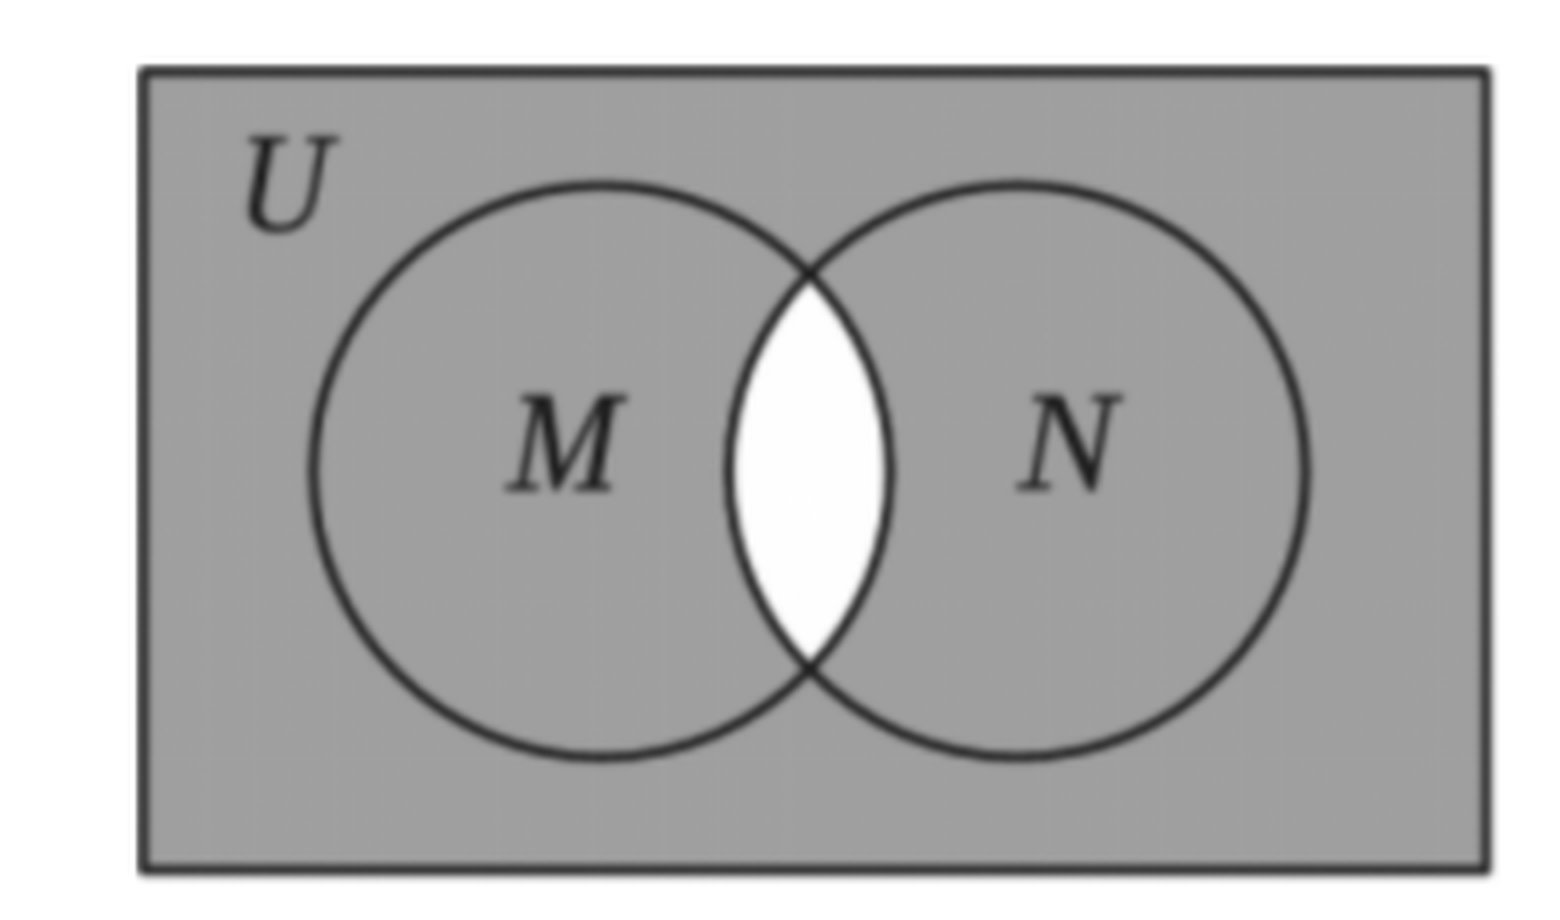
\includegraphics[width=0.40\textwidth]{figures/gao145_q14.png}
\end{center}

\ifanswer
\solbegin
\step{由韦恩图得图中白色区域为集合 $M\cap N$，所以阴影部分表示的集合为 $\overline{M\cap N}$.}
\step{故选 $D$.}
\solend
\fi

% === Q15 ===
\item 已知 $x>-2$，则 $x+\dfrac{1}{x+2}$ 的最小值为\mbox{（\quad）}

\keepwithprev
A. 3\qquad B. 2\qquad C. 1\qquad D. 0

\ifanswer
\solbegin
\step{$x>-2$，则 $x+2>0$，}
\step{所以 $x+\dfrac{1}{x+2}=(x+2)+\dfrac{1}{x+2}-2\geqslant2\sqrt{(x+2)\cdot\dfrac{1}{x+2}}-2=0$，}
\step{当且仅当 $x+2=\dfrac{1}{x+2}$，即 $x=-1$ 时取等号，所以 $x+\dfrac{1}{x+2}$ 的最小值为 $0$.}
\step{故选 $D$.}
\solend
\fi

% 第 16 题：题干在 05 页、解析续至 06 页；两幅数轴标根波浪曲线是【解析】内配图，
% 仅答案版出，放在答案版条件块内 \solbegin 的 \step 之间（照 高一73 第 16 题成例）
\item 关于 $x$ 的不等式 $\dfrac{(x-a)(x-2)^2}{(x-1)(x-5)}\leqslant0$ 的解集中恰有 3 个正整数，则实数 $a$ 的取值范围是\mbox{（\quad）}

\keepwithprev
A. $(-\infty,3]\cup[7,8)$\qquad B. $(-\infty,3)\cup[7,8)$\qquad C. $(-\infty,3]\cup(7,8]$\qquad D. $(-\infty,3)\cup(7,8]$

\ifanswer
\solbegin
\step{由题意，不等式 $\dfrac{(x-a)(x-2)^2}{(x-1)(x-5)}\leqslant0$，}
\step{可化为 $\begin{cases}(x-1)(x-2)^2(x-5)(x-a)\leqslant0\\x\ne1\text{且}x\ne5\end{cases}$，由数轴标根法，}
\step{当 $a=3$ 时，}
\begin{center}
% a=3 数轴标根图取 06 页，去粉色水印、去色、4× LANCZOS 放大；仅答案版出
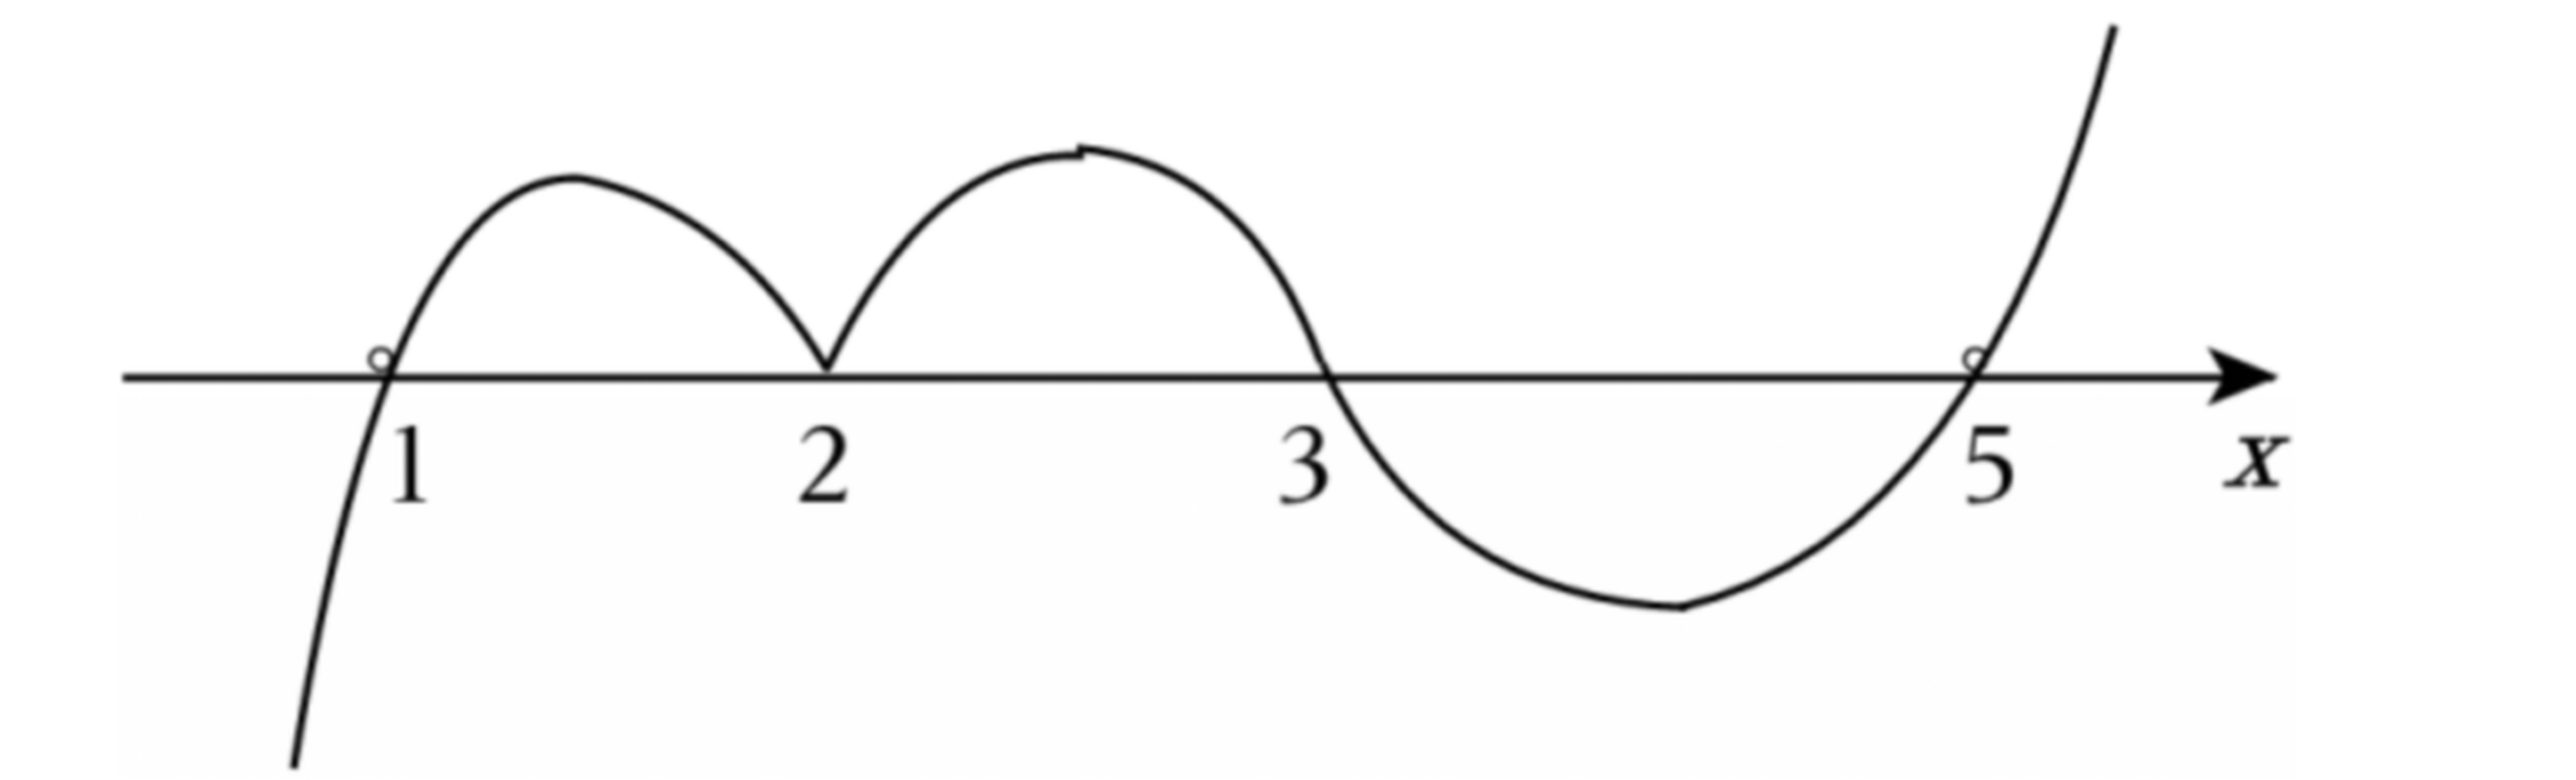
\includegraphics[width=0.62\textwidth]{figures/gao145_q16_a3.png}
\end{center}
\step{得不等式的解集为 $\{x\mid x<1\text{ 或 }x=2\text{ 或 }3\leqslant x<5\}$，}
\step{对应的正整数解为 $2$，$3$，$4$，满足题意，故排除 $B$、$D$；}
\step{当 $a=7$ 时，}
\begin{center}
% a=7 数轴标根图取 06 页，去粉色水印、去色、4× LANCZOS 放大；仅答案版出
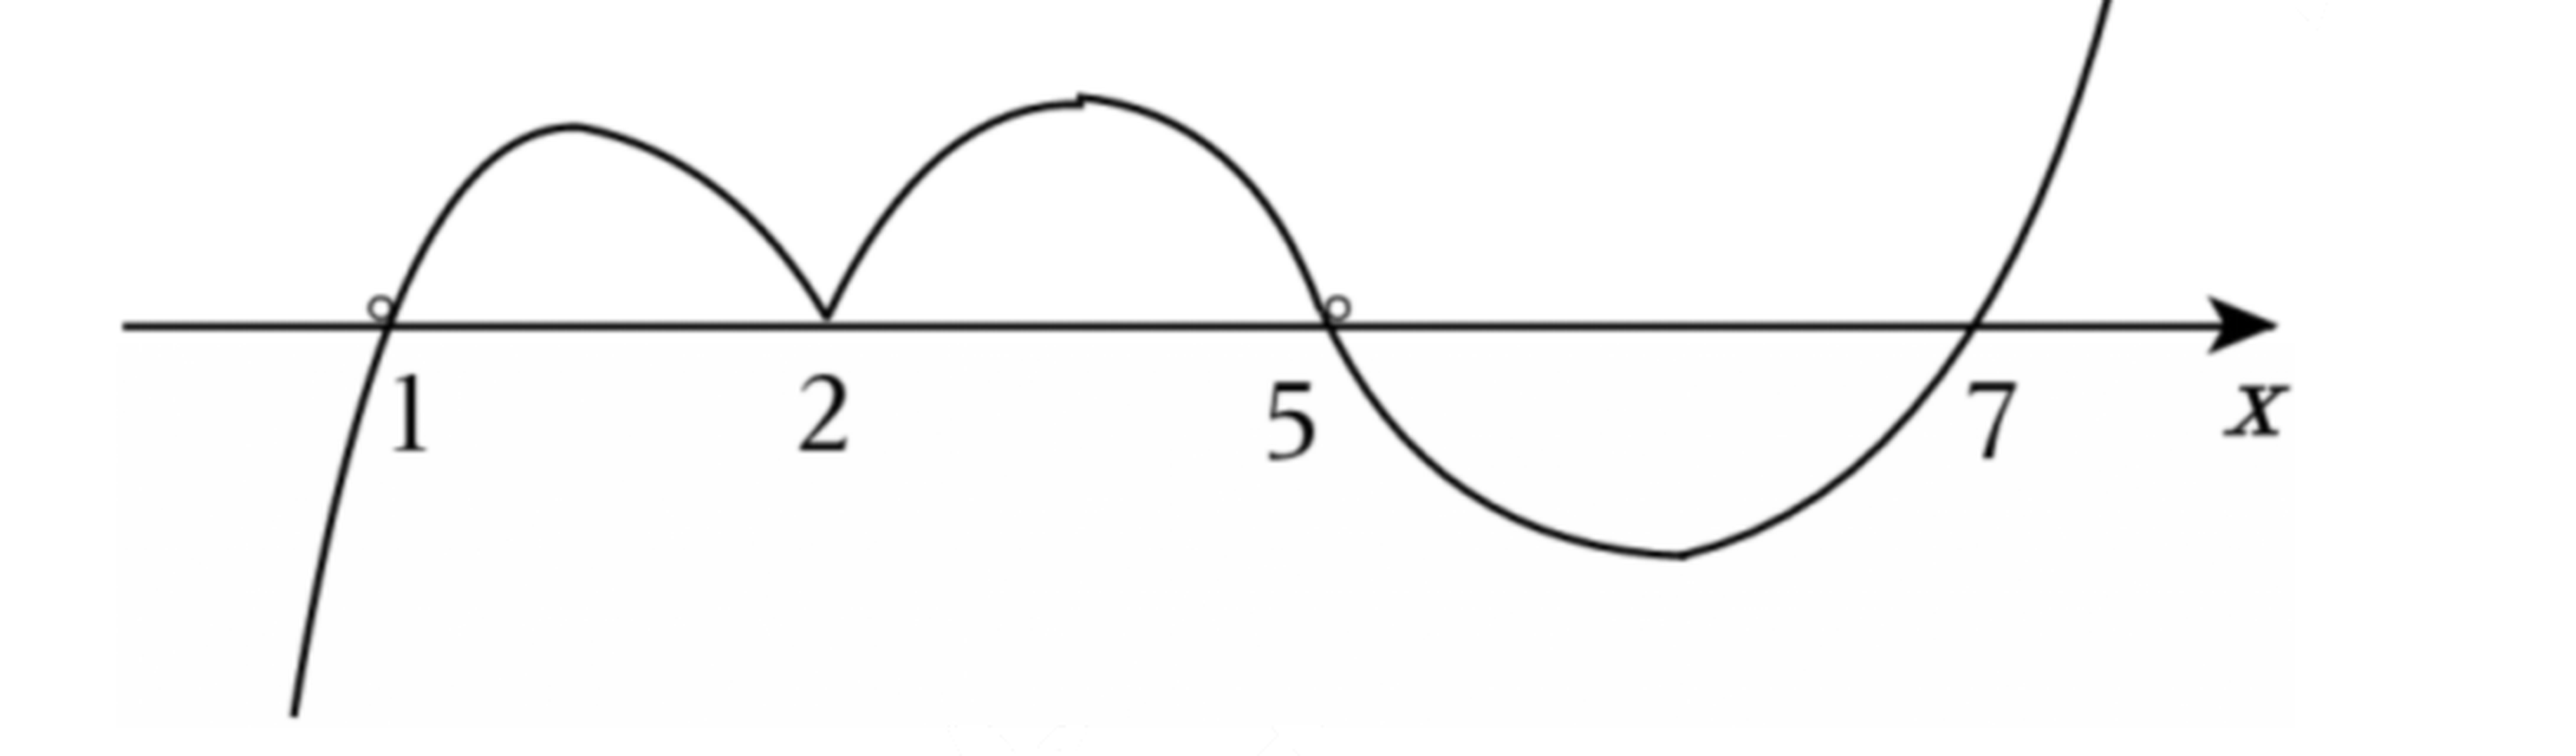
\includegraphics[width=0.62\textwidth]{figures/gao145_q16_a7.png}
\end{center}
\step{得不等式的解集为 $\{x\mid x<1\text{ 或 }x=2\text{ 或 }5<x\leqslant7\}$，}
\step{对应的正整数解为 $2$，$6$，$7$，满足题意，故 $A$ 正确，$C$ 错误.}
\step{故选 $A$.}
\solend
\fi

\end{enumerate}

\bigsec{三、解答题}

\begin{enumerate}
\setcounter{enumi}{16}

% 第 17 题：题干在 06 页、解析续至 07 页，按印刷行断，共 7 行；
% "lg(10÷5)" 的除号照录 \div
\item (1) 已知 $a+a^{-1}=6$，求 $a^2+a^{-2}$ 及 $a^{\frac12}-a^{-\frac12}$ 的值；

(2) 已知 $\lg5=a$，$\lg6=b$，用 $a$、$b$ 分别表示 $\lg2$、$\lg3$、$\lg300$ 和 $\log_{12}15$.

\ifanswer
\solbegin
\step{(1) 因为 $a+a^{-1}=6$，}
\step{所以 $a^2+a^{-2}=(a+a^{-1})^2-2\cdot a\cdot a^{-1}=6^2-2=34$，}
\step{因为 $\left(a^{\frac12}-a^{-\frac12}\right)^2=a-2+a^{-1}=6-2=4$，所以 $a^{\frac12}-a^{-\frac12}=\pm2$；}
\step{(2) $\lg2=\lg(10\div5)=\lg10-\lg5=1-a$，}
\step{$\lg3=\lg(6\div2)=\lg6-\lg2=b-(1-a)=a+b-1$，}
\step{$\lg300=\lg(3\times10^2)=\lg3+\lg10^2=a+b-1+2=a+b+1$，}
\step{所以 $\log_{12}15=\dfrac{\lg15}{\lg12}=\dfrac{\lg3+\lg5}{\lg3+\lg2^2}=\dfrac{a+b-1+a}{a+b-1+2(1-a)}=\dfrac{2a+b-1}{b-a+1}$.}
\solend
\fi

% 第 18 题：题干在 07 页、解析续至 08 页（2 问、分类讨论很长），按印刷行断共 25 行；
% 本卷 Q18 用"图像"（Q13/Q14 用"图象"），逐处照录不统一
\item 已知 $f(x)=(m^2-3m+1)x^{m^2-4m-1}$，$y=f(x)$ 为幂函数且在 $(0,+\infty)$ 上是严格减函数.

(1) 求实数 $m$ 的值以及相应的函数表达式；

(2) 若 $y=f(x)$ 的图像关于 $y$ 轴对称，解关于 $x$ 的不等式 $(x+2)^{1-m}<(3x-1)^{1-m}$.

\ifanswer
\solbegin
\step{(1) 由幂函数的定义得 $m^2-3m+1=1$，}
\step{整理得 $m^2-3m=0$，解得 $m=0$ 或 $m=3$，}
\step{由于 $y=f(x)$ 在 $(0,+\infty)$ 上为严格减函数，}
\step{因此幂函数的指数需满足 $m^2-4m-1<0$，}
\step{当 $m=3$ 时，指数为 $3^2-4\times3-1=-4<0$，满足严格递减条件，}
\step{此时函数表达式为 $f(x)=x^{-4}$，}
\step{当 $m=0$ 时，指数为 $0^2-4\times0-1=-1<0$，满足严格递减条件，}
\step{此时函数表达式为 $f(x)=x^{-1}$，}
\step{所以满足条件的实数 $m$ 为 $0$ 或 $3$，}
\step{对应的函数表达式分别为 $f(x)=x^{-1}$、$f(x)=x^{-4}$；}
\step{(2) 函数图像关于 $y$ 轴对称即函数为偶函数，}
\step{对于 $f(x)=x^{-1}=\dfrac1x$，定义域为 $(-\infty,0)\cup(0,+\infty)$，}
\step{满足 $f(-x)=-f(x)$，为奇函数，图像关于原点对称，}
\step{不满足关于 $y$ 轴对称的条件；}
\step{对于 $f(x)=x^{-4}=\dfrac{1}{x^4}$，定义域为 $(-\infty,0)\cup(0,+\infty)$，}
\step{满足 $f(-x)=f(x)$，为偶函数，图像关于 $y$ 轴对称，}
\step{因此符合条件的 $m$ 值为 $3$，}
\step{将 $m=3$ 代入关于 $x$ 的不等式 $(x+2)^{1-m}<(3x-1)^{1-m}$，}
\step{得 $(x+2)^{1-3}<(3x-1)^{1-3}$，即 $(x+2)^{-2}<(3x-1)^{-2}$，}
\step{因为负指数幂的底数不能为 $0$，所以 $x+2\ne0$ 且 $3x-1\ne0$，}
\step{即 $x\ne-2$ 且 $x\ne\dfrac13$，}
\step{不等式可变形为 $\dfrac{1}{(x+2)^2}<\dfrac{1}{(3x-1)^2}$，}
\step{整理得 $(3x-1)^2<(x+2)^2$，即 $8x^2-10x-3<0$，}
\step{解得 $-\dfrac14<x<\dfrac32$，又 $x\ne-2$ 且 $x\ne\dfrac13$，}
\step{所以不等式的解集为 $\left(-\dfrac14,\dfrac13\right)\cup\left(\dfrac13,\dfrac32\right)$.}
\solend
\fi

% 第 19 题：题干在 08 页、解析续至 09 页，按印刷行断，共 14 行；
% 判别式 cases 块内"△=4a²−16a<0"原卷印扁等边三角 \triangle
%（放大 09 页 zz09_delta.png 与 Q12 高 \Delta 并排确认），逐处照录不统一
\item 已知 $f(x)=ax^2+2ax+4$，$a\in\R$.

(1) 若关于 $x$ 的不等式 $f(x)>0$ 在实数集 $\R$ 上恒成立，求实数 $a$ 的取值范围；

(2) 当 $a<0$ 时，解关于 $x$ 的不等式 $f(x)>(a+1)x+5$.

\ifanswer
\solbegin
\step{(1) 由题意得，关于 $x$ 的不等式 $f(x)>0$ 在实数集 $\R$ 上恒成立，}
\step{即 $ax^2+2ax+4>0$ 在实数集 $\R$ 上恒成立，}
\step{当 $a=0$ 时，不等式为 $4>0$ 恒成立，符合题意；}
\step{当 $a\ne0$ 时，则 $\begin{cases}a>0\\\triangle=4a^2-16a<0\end{cases}$，解得 $0<a<4$.}% 判别式原卷印扁等边三角 $\triangle$，照录
\step{综上所述，实数 $a$ 的取值范围为 $[0,4)$.}
\step{(2) $f(x)=ax^2+2ax+4$，}
\step{当 $a<0$ 时，不等式 $f(x)>(a+1)x+5$ 即为 $ax^2+(a-1)x-1>0$，}
\step{即 $(ax-1)(x+1)>0$，即 $\left(x-\dfrac1a\right)(x+1)<0$，}
\step{当 $a<-1$，即 $\dfrac1a>-1$ 时，解得 $-1<x<\dfrac1a$；}
\step{当 $a=-1$，即 $\dfrac1a=-1$ 时，解得 $x\in\varnothing$；}
\step{当 $-1<a<0$，即 $\dfrac1a<-1$ 时，解得 $\dfrac1a<x<-1$.}
\step{综上所述，当 $a<-1$ 时，不等式的解集为 $\left\{x\mid -1<x<\dfrac1a\right\}$；}
\step{当 $a=-1$ 时，不等式的解集为 $\varnothing$；}
\step{当 $-1<a<0$ 时，不等式的解集为 $\left\{x\mid \dfrac1a<x<-1\right\}$.}
\solend
\fi

% 第 20 题：菜园靠墙图为题目配图（三版都出），题干写"如图"；
% 题干在 09 页（含图）、解析续至 10 页，按印刷行断，共 13 行
\needvspace{8cm}
\item 如图，某人计划用篱笆围成一个一边靠墙（墙足够长）的矩形菜园. 设菜园的长为 $x$ 米，宽为 $y$ 米.

\begin{center}
% 矩形菜园靠墙图取 09 页右下，去粉色水印、去色、4× LANCZOS 放大
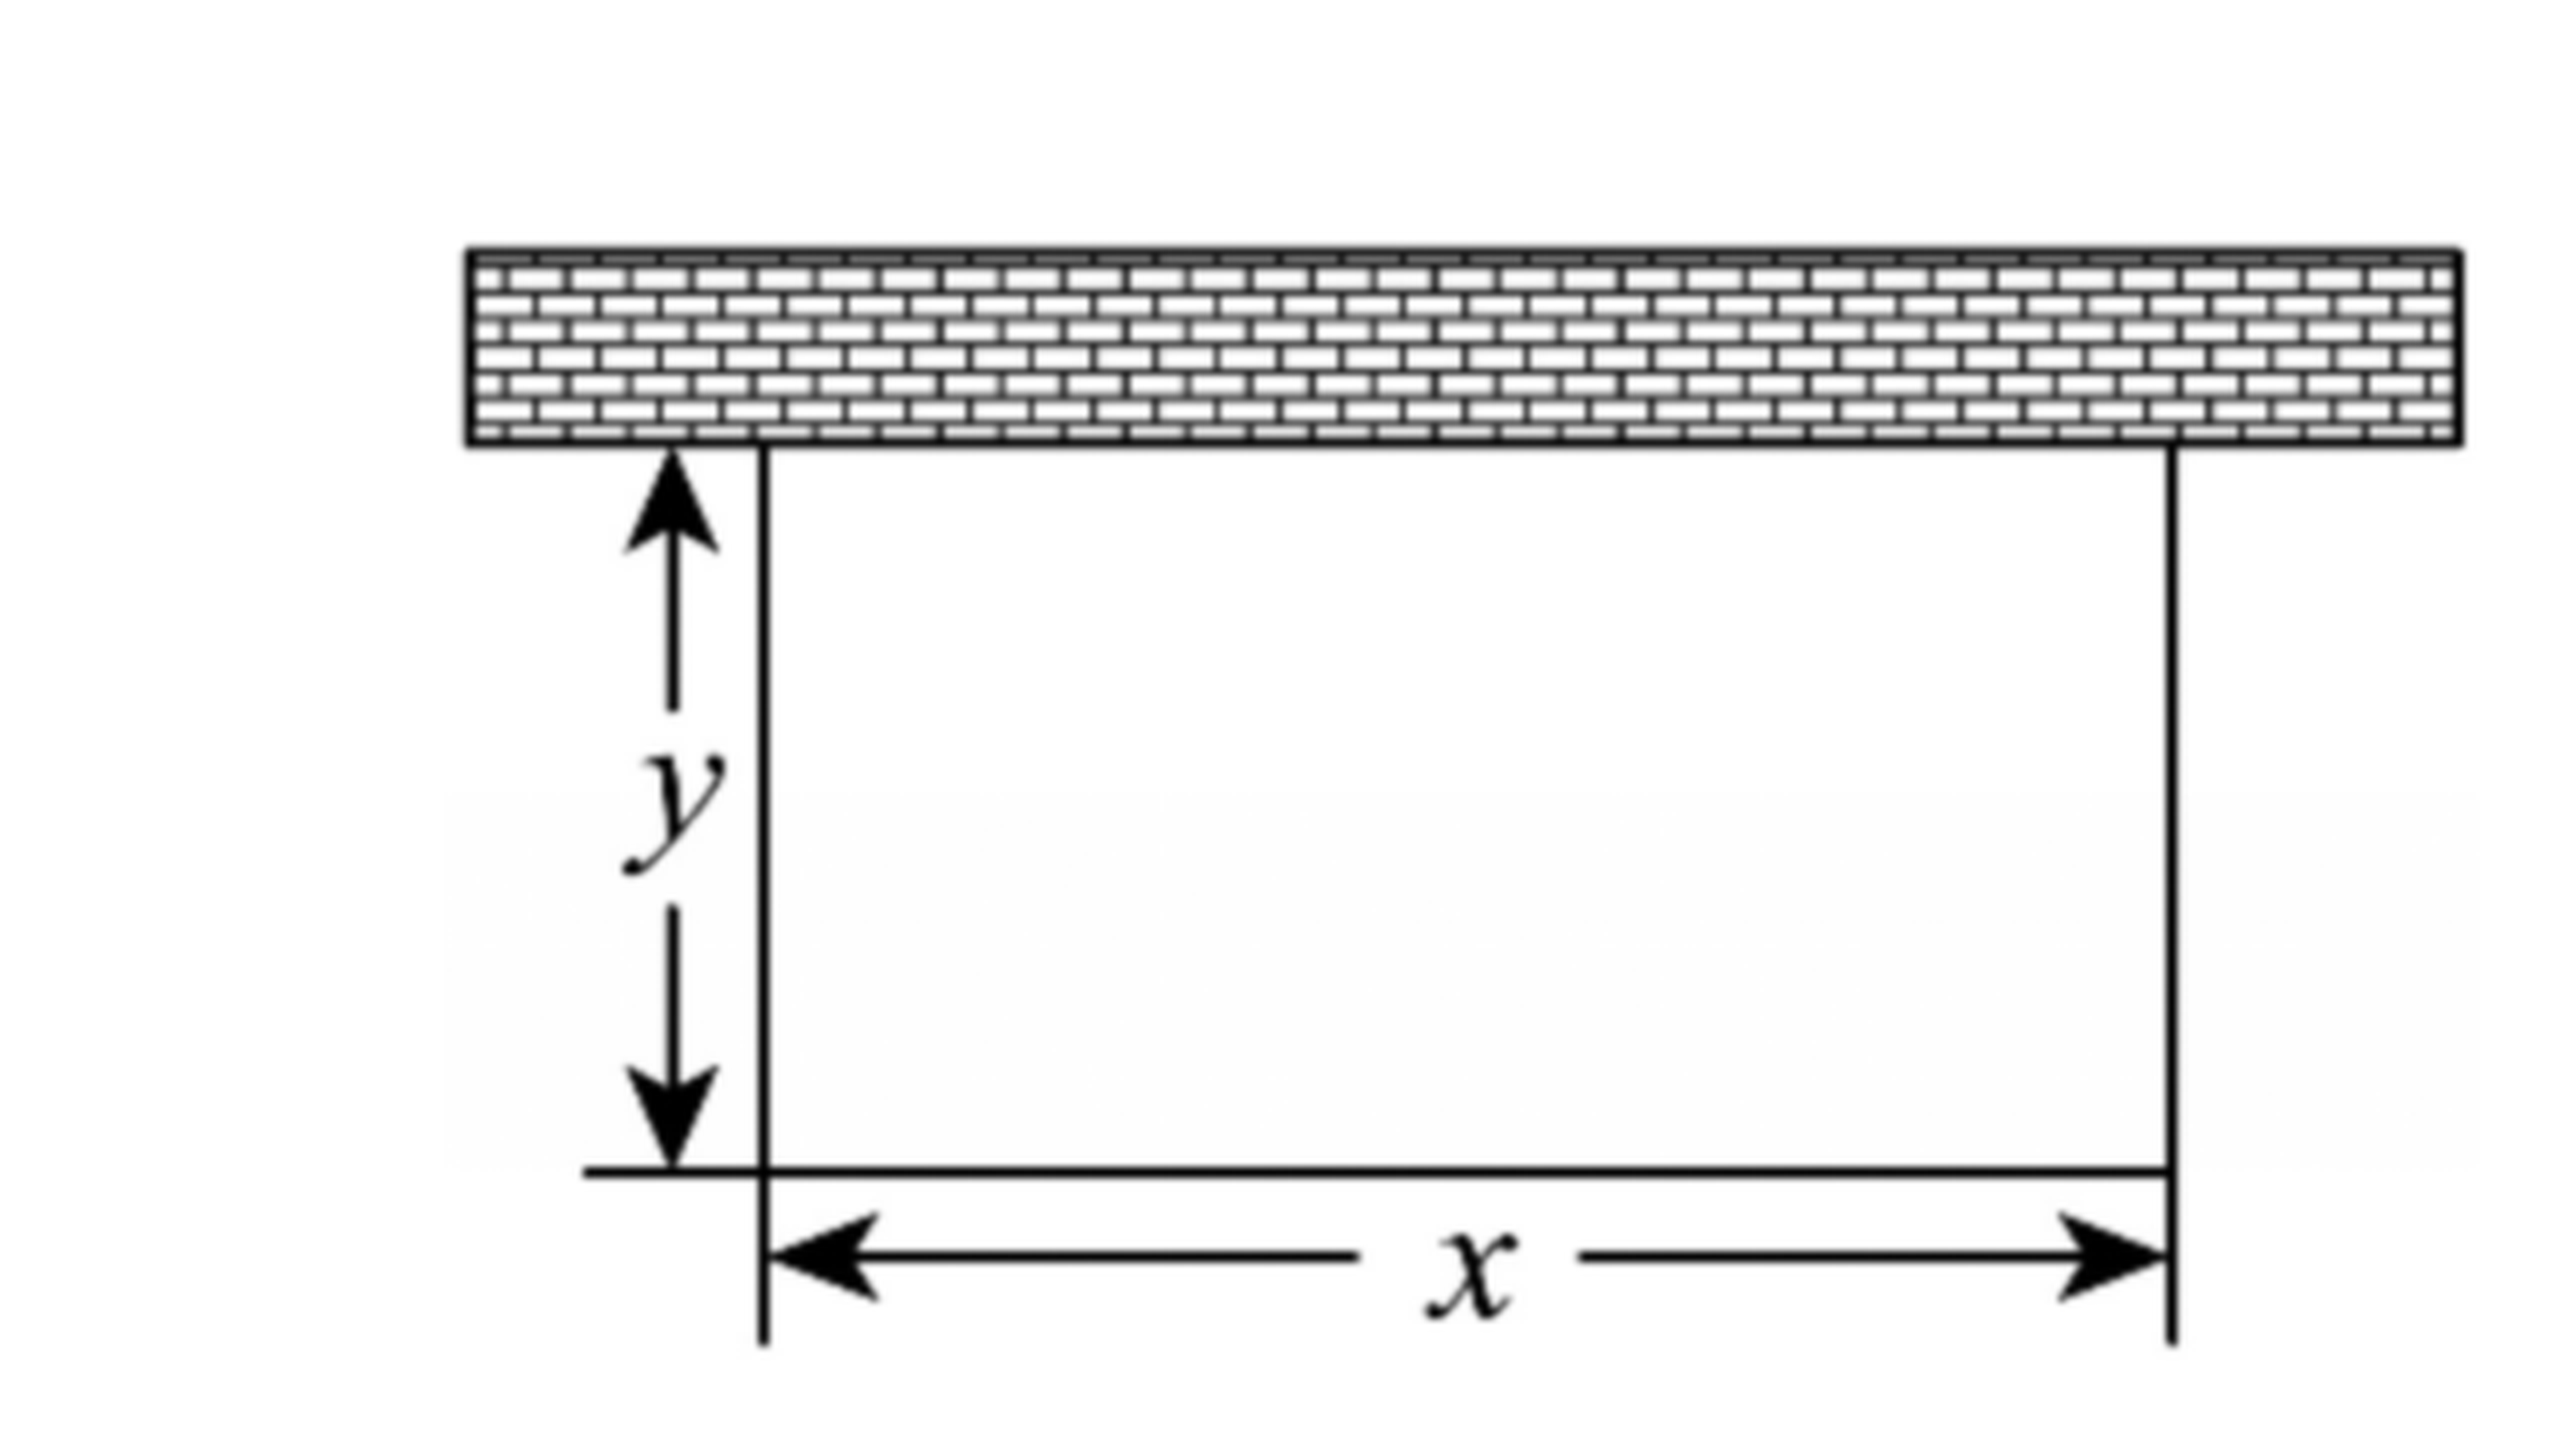
\includegraphics[width=0.55\textwidth]{figures/gao145_q20.png}
\end{center}

(1) 若菜园面积为 72 平方米，则 $x$、$y$ 为何值时，所用篱笆总长最小？

(2) 若 $x$、$y$ 满足 $x+y-xy+63=0$，则菜园面积最小为多少平方米？

\ifanswer
\solbegin
\step{(1) 由题意得，菜园的面积 $S=xy=72$，且 $x>0$，$y>0$，}
\step{所用篱笆总长 $L=x+2y$，}
\step{由基本不等式得 $x+2y\geqslant2\sqrt{x\cdot2y}=2\sqrt{2xy}=2\sqrt{2\times72}=24$，}
\step{当且仅当 $x=2y$ 时取等号，}
\step{联立 $\begin{cases}xy=72\\x=2y\end{cases}$，解得 $\begin{cases}x=12\\y=6\end{cases}$，}
\step{所以当 $x=12$，$y=6$ 时，所用篱笆总长最小；}
\step{(2) 由题意得 $x>0$，$y>0$，且满足 $x+y-xy+63=0$，即 $x+y=xy-63$，}
\step{由基本不等式得 $x+y\geqslant2\sqrt{xy}$，当且仅当 $x=y$ 时取等号，}
\step{所以 $xy-63\geqslant2\sqrt{xy}$. 令 $t=\sqrt{xy}(t>0)$，则 $xy=t^2$，}
\step{上述不等式可化为 $t^2-2t-63\geqslant0$，即 $(t-9)(t+7)\geqslant0$，}
\step{因为 $t>0$，所以 $t+7>0$，故 $t-9\geqslant0$，解得 $t\geqslant9$，所以 $\sqrt{xy}\geqslant9$，}
\step{即 $xy\geqslant81$，当且仅当 $x=y=9$ 时取等号，此时满足 $9+9-81+63=0$，}
\step{所以菜园面积最小为 81 平方米.}
\solend
\fi

% 第 21 题：题干在 10 页、解析续至 11 页（3 问、分类讨论很长），按印刷行断共 22 行；
% 末行"故第 2026 个元素是 2700 之后第一个属于 A 的数，即 2701." 为全卷收尾，
% 无 Q22/Q23、无附加题节；数集 Z/N* 按全稿惯例改 \Z/\N^*
\item 已知集合 $A=\{x\mid x=m^2-n^2$，$m$、$n\in\Z\}$.

(1) 求证：任何奇数 $2k+1(k\in\Z)$ 都是集合 $A$ 中的元素；

(2) 判断偶数 $4k-2(k\in\Z)$ 是否为集合 $A$ 的元素？请说明理由；

(3) 若将集合 $A$ 中的正整数由小到大排列，求出集合 $A$ 中第 2026 个正整数.

\ifanswer
\solbegin
\step{(1) 因为 $x=(k+1)^2-k^2=2k+1(k\in\Z)$，}
\step{所以任何奇数 $2k+1(k\in\Z)$ 都属于集合 $A$；}
\step{(2) 偶数 $4k-2(k\in\Z)$ 不是集合 $A$ 的元素，理由如下：}
\step{由题意得 $x=m^2-n^2=(m-n)(m+n)$，}
\step{当 $m$、$n$ 均为奇数时，设 $m=2k_1+1$，$n=2k_2+1(k_1$、$k_2\in\Z)$，}
\step{则 $m^2-n^2=(2k_1+1)^2-(2k_2+1)^2=(2k_1-2k_2)(2k_1+2k_2+2)$}
\step{$=4(k_1-k_2)(k_1+k_2+1)$，}
\step{因为 $k_1$、$k_2\in\Z$，所以 $k_1-k_2\in\Z$，$k_1+k_2+1\in\Z$，}
\step{从而 $m^2-n^2$ 为 $4$ 的倍数；}
\step{当 $m$、$n$ 均为偶数时，设 $m=2k_1$，$n=2k_2(k_1$、$k_2\in\Z)$，}
\step{$m^2-n^2=4k_1^2-4k_2^2=4(k_1^2-k_2^2)$ 为 $4$ 的倍数；}
\step{当 $m$、$n$ 为一个偶数一个奇数时，不妨设 $m$ 为偶数，$n$ 为奇数，}
\step{设 $m=2k_1$，$n=2k_2+1(k_1$、$k_2\in\Z)$，}
\step{则 $m^2-n^2=4k_1^2-(2k_2+1)^2=4(k_1^2-k_2^2-k_2)-1$ 为奇数.}
\step{无论哪种情况均不满足 $4k-2(k\in\Z)$，}
\step{故偶数 $4k-2(k\in\Z)$ 不是集合 $A$ 的元素；}
\step{(3) 由前两问得，$4$ 的倍数和奇数属于集合 $A$ 中的元素，}
\step{令集合 $A$ 中的正整数元素为 $4k-3$、$4k-1$、$4k(k\in\N^*)$，}
\step{对任意的 $k\in\N^*$，连续的 $4$ 个整数 $4k-3$、$4k-2$、$4k-1$、$4k$ 中}
\step{有三个数 $4k-3$、$4k-1$、$4k$ 都在集合 $A$ 中，}
\step{因为 $2026=3\times675+1$，所以集合 $A$ 中第 $2025$ 个元素为 $4\times675=2700$，}
\step{故第 2026 个元素是 2700 之后第一个属于 $A$ 的数，即 2701.}
\solend
\fi

\end{enumerate}

\end{document}
"
% 紧凑版：xelatex "\def\iscompact{1}% 高一145_市二中学_期中.tex
%   —— 高一上数学"2026-2027 年市二中学高一上期中"（试卷版/答案版/紧凑版）
% 试卷版：xelatex 高一145_市二中学_期中.tex
% 答案版：xelatex "\def\isanswer{1}\input{高一145_市二中学_期中.tex}"
% 紧凑版：xelatex "\def\iscompact{1}\input{高一145_市二中学_期中.tex}"
%
% ① 原始材料：微信公众号"魔都数学加油站"文章，连载"27学年高一145"，原文标题
% "27学年高一145——2026-2027年上海市市二中学高一上期中"；
% 原文链接：https://mp.weixin.qq.com/s/6V-i9KE0GWodC-wmd5z8nQ 。
% 正文为 11 张 PNG 页（01/02/03/08/10/11 为 4762×6735，04/05/06/07/09 为 2560×3620，
% 同一篇各页分辨率不同，逐页按各自分辨率裁图核对，别按预览比例换算裁框）。
% 题目下印【答案】或【解析】，为混合体例讲评版：Q3 只印【答案】、无【解析】，其余
% 18 题印【解析】。题目、解析均据原图转录；卷面粉红色水印"魔都数学加油站"及
% 公众号页脚未录入。
% 全卷插图情况（逐页通读 11 页确认，题干写"如图"处均配有图）：
%   · Q14 韦恩图（05 页右侧，全集 U 矩形＋两圆 M/N＋白色交集、灰色阴影＋U/M/N 标注）：
%     题目配图（选择题选项旁），三版都出，裁自 05 页去水印去色 4× 放大存
%     figures/gao145_q14.png；
%   · Q16 两幅数轴标根波浪曲线（06 页，a=3 与 a=7 各一幅，标根法画
%     (x-1)(x-2)^2(x-5)(x-a)≤0 的符号曲线）：【解析】内的配图，仅答案版出，
%     裁 figures/gao145_q16_a3.png / figures/gao145_q16_a7.png（或合并一张），
%     放在答案版条件块内 \solbegin 的 \step 之间（照 高一73 第 16 题成例）；
%   · Q20 矩形菜园靠墙图（09 页右下，灰色砖墙＋矩形菜园＋x/y 标注＋箭头）：
%     题目配图，三版都出，裁自 09 页去水印去色 4× 放大存 figures/gao145_q20.png；
%   其余各页逐页确认无其它题目配图、无表格、亦无"题干写如图而源码漏图"一处。
%
% 卷首标题：原卷印作"2026-2027 年市二中学高一上期中"，年份区间按全稿惯例排 en dash；
% 原卷卷面未印副标题，本稿按同期中卷（高一140／141／143／144）知识模块口径补出
% "集合与常用逻辑用语、不等式、函数"。
%
% 题号体例：本卷共 19 题——一、填空题 3—12（10 题）、二、选择题 13—16（4 题）、
% 三、解答题 17—21（5 题）。三节分别 \setcounter{enumi}{2}／{12}／{16}。
% 原卷从第 3 题起、无第 1、2 题，本稿保留原题号；全卷无附加题节。
%
% ② 与原卷的排版差异：
%   ① 原文从第 3 题起，本稿保留原题号；共 19 题三节；
%   ② 混合体例：原卷 Q3 只印【答案】、无【解析】（"第一步应假设___。
%      【答案】x≤2 或 y≤2"），按 高一140 第 5 题成例提 \ans{}、不补造解析；
%      其余 18 题印【解析】，用 \solbegin…\solend，选择题答案在解析末句"故选 X"
%      （Q13 选 B、Q14 选 D、Q15 选 D、Q16 选 A，逐个放大原图核实）、
%      题干括号 \mbox{（\quad）} 留空、不另提 \ans{}；填空／解答答案落在解析里；
%      答案版【答案】/【解析】标记数 = 19（1 个 \ans ＋ 18 个 \solbegin）= 全卷题数；
%   ③ 原卷卷面未印副标题，本稿按知识模块口径补出；
%   ④ 原卷填空横线按全稿惯例排 \blankline[4.4em]；选择题括号排 \mbox{（\quad）}、
%      选项段前按惯例加 \keepwithprev；解答题不留作答区、不加 \anspace
%      （原卷为讲评版，与 129／131／132／133／136／140／141／143／144 同）；
%   ⑤ 数集：Q9"a、b∈R"、Q12"a∈R"、Q21"m、n∈Z""k∈Z""k∈N*"等原卷印
%      斜体或黑板粗体 R/Z/N，按全稿惯例统一改 \R／\Z／\N^*；绝对值排 \lvert…\rvert，
%      集合描述竖线排 \mid；不等号按全稿惯例排 \leqslant／\geqslant；
%      补集照原卷上划线排 \overline{M}／\overline{N}（Q14 选项 B/C/D 逐处核）；
%      空集记号 \varnothing；\subset（单线⊂）与 \subseteq（带下划线⊆）逐处照录不统一；
%   ⑥ 子题标号 (1)(2)(3) 原卷印半角括号照录；圈数字进数学式用 \text{①}（否则 FONTCHK 挂）；
%      \left…\right 不得拆到不同 $…$ 组；cases 块整体算一个印刷行；
%   ⑦ 题干／解析中的中文弯引号按原卷照录（Q3"若 x+y>4，则 x>2 且 y>2"、
%      Q11"a₁/a₂=b₁/b₂""M=N"、选填"充分非必要""必要非充分""充要""既非充分也非必要"
%      等，含引号内空格），注释内一律 ASCII 引号；数学式内 CJK 用 \text{}；
%   ⑧ 半角逗号在数学组之间是全稿惯例、非笔误（如 Q5"x₁+x₂=6，x₁x₂=√3"、
%      Q7"a>1，b>1"、指数／对数式内逗号），逐处照录别改全角；行末西文句点照录为
%      ASCII `.`；行中全角逗号／顿号照录；
%   ⑨ "图像／图象"逐处照录不统一（Q18"图像关于 y 轴对称"等，核全卷）；
%   ⑩ 判别式 Δ/△ 混用是照录项：Q12 解析"Δ=a²−4a²(2a−3)>0"、
%      Q19 解析"Δ=4a²−16a<0"等，放大原图判断是高 \Delta（等腰偏高、高>宽）
%      还是扁 \triangle，逐处照录不得统一（参照 高一142／144 头注④口径）；
%   ⑪ 一条 \step = 原卷解析的一个印刷行，cases 块整体算一个印刷行；别把原卷折行
%      并起来、别把一行拆多条。Q6 分段讨论、Q12 三个 cases 条件组、Q16 数轴标根、
%      Q18／Q19 分类讨论、Q21 三问均按印刷行逐条断，不丢行；
%   ⑫ Q14 韦恩图为"题干＋选项＋图"整块，加 \needvspace 守卫推走（守卫放 \item 之前，
%      见 高一140 Q14、高一144 Q17 成例与切页审计 B 类坑）；Q20 菜园图同理；
%      三版切页审计均"合计异常：无"；
%   ⑬ 跨页续印按题合并：Q3/4/5/6 在 01 页（Q6 解析续 02 页顶）；Q7/8/9/10 在 02 页
%      （Q10 解析续 03 页）；Q11/12 在 03 页（Q12 解析续 04 页，很长）；
%      Q13 在 04 页末、解析在 05 页顶；Q14/15/16 在 05 页（Q16 解析续 06 页含两幅数轴图）；
%      Q17 在 06 页、解析续 07 页；Q18 在 07 页、解析续 08 页；Q19 在 08 页、解析续 09 页；
%      Q20 在 09 页（含菜园图）、解析续 10 页；Q21 在 10 页、解析续 11 页
%      （末页收尾"故第 2026 个元素是 2700 之后第一个属于 A 的数，即 2701."、
%      无 Q22/Q23、无附加题节）。本稿按题连排，不丢行、不并折行；
%   ⑭ 原卷解析内若有红色"法一／法二"之类小标题，按全稿惯例排 \stepm{标签}{…}
%      （黑体着色、不引入红色、不改 common.sty），头注注明；水印"魔都数学加油站"
%      红色不录入。
%
% ③ 行数复核：一条 \step／\stepm = 原卷解析的一个印刷行，cases 块作一个印刷行计。
%   逐题数（主会话逐页核对定稿）：Q3：0（只印【答案】、提 \ans{}，不计入 \step 账）；
%   Q4：3；Q5：2；Q6：10；Q7：3；Q8：3；Q9：2；Q10：7；Q11：4；Q12：12；
%   Q13：2；Q14：2；Q15：4；Q16：9；Q17：7；Q18：25；Q19：14；Q20：13；Q21：22。
%   合计 144 条 \step（本卷无 \stepm：解析内无红色"法一／法二"类小标题），
%   与原卷逐题印刷行相等。全卷 18 题设 \solbegin…\solend ＋ Q3 一处 \ans{}，
%   答案版【答案】/【解析】标记数 = 19 = 全卷题数。
%
% ④ 判别式／子集符号结论（逐处放大原图照录、不得统一，主会话像素级复核）：
%   判别式全卷 2 处、两形混用逐处照录不统一（参照 高一142／144 头注④口径）：
%     · Q12 解析 cases 块"Δ=a²−4a²(2a−3)>0" 原卷印等腰偏高粗三角（高>宽），
%       照录 \Delta（放大 04 页 /tmp/gao145s2/main_q12_delta.png 确认）；
%     · Q19 解析 cases 块"△=4a²−16a<0" 原卷印扁等边空心三角（宽≈高、细线），
%       照录 \triangle（放大 09 页 /tmp/gao145s2/main_q19_delta.png 确认）。
%   子集／补集：Q14 选项 A `M\cup N`、B `M\cap\overline{N}`（上划线只在 N 上）、
%   C `\overline{M\cup N}`（罩整个 M∪N）、D `\overline{M\cap N}`（罩整个 M∩N，
%   非 \overline{M}\cap N；放大 05 页 /tmp/gao145s2/main_q14_opts.png 确认），
%   阴影为灰色区域＝全集减白色交集，答案 D，照录 \overline{M\cap N}；
%   全集卷无 \subset／\subseteq 混用（本卷集合题用 \cup／\cap／\overline{}）；
%   空集 \varnothing（Q19 解析 x∈\varnothing）；数集 \R／\Z／\N^* 归一见 ② ⑤。
%
% ⑤ 存疑照录（放大原图确认，照录未改、正文对应处另有 % 注）：
%   1. Q3 题干"若 x+y>4，则 x>2 且 y>2" 后"时"前留一空格、弯引号内空格照录；
%      该卷混合体例（Q3 只印【答案】、提 \ans{}）见 ② ②。
%   2. Q4／Q5 解析中的"1，3，5 和 6"、"x₁+x₂=6,x₁x₂=√3" 等半角／全角逗号
%      逐处照原卷（放大 01 页确认），数学式内半角逗号为全稿惯例、非笔误。
%   3. Q14 选项 D 上划线罩住整个 M∩N（而非仅罩 M），照录 \overline{M\cap N}。
%   4. Q12 判别式高 \Delta 与 Q19 判别式扁 \triangle 两形混用，逐处照录不统一（见 ④）。
%   全卷除此 4 类外未发现其它笔误／自相矛盾处。
%
% ⑥ 跨页续印按题合并说明：见 ② ⑬。
%
\documentclass[a4paper,11pt]{article}
\usepackage{common}

\begin{document}

\examtitlest[3]{2026--2027 年市二中学高一上期中}{集合与常用逻辑用语、不等式、函数}

\bigsec{一、填空题}

\begin{enumerate}
\setcounter{enumi}{2}

% 第 3 题：原卷只印【答案】、无【解析】（放大 01 页确认），按 高一140 第 5 题成例
% 提 \ans{}、不补造解析；题干中文弯引号与"时"前空格照录
\item 用反证法证明命题：“若 $x+y>4$，则 $x>2$ 且 $y>2$” 时，第一步应假设\blankline[4.4em].

\ifanswer
\ans{$x\leqslant2$ 或 $y\leqslant2$}
\fi

% === Q4 ===
\item 设集合 $M$ 满足 $\{1,3,5,6\}\cup M=\{1,2,3,4,5,6\}$，则满足条件的所有 $M$ 的个数为\blankline[4.4em].

\ifanswer
\solbegin
\step{集合 $M$ 满足 $\{1,3,5,6\}\cup M=\{1,2,3,4,5,6\}$，}
\step{则 $M$ 中必含有 $2$ 和 $4$，$1$，$3$，$5$ 和 $6$ 可以选也可不选，}
\step{则满足条件的所有 $M$ 的数目相当于集合 $\{1,3,5,6\}$ 的子集的个数 $2^4=16$.}
\solend
\fi

% === Q5 ===
\item 已知方程 $x^2-6x+\sqrt3=0$ 的两根为 $x_1$ 和 $x_2$，则 $(x_1-x_2)^2=$\blankline[4.4em].

\ifanswer
\solbegin
\step{因为方程 $x^2-6x+\sqrt3=0$ 的两根为 $x_1$ 和 $x_2$，所以 $x_1+x_2=6,x_1x_2=\sqrt3$，}% 数学式内半角逗号为全稿惯例，照录
\step{所以 $(x_1-x_2)^2=(x_1+x_2)^2-4x_1x_2=36-4\sqrt3$.}
\solend
\fi

% 第 6 题：题干在 01 页，解析续至 02 页顶（末 2 行），按印刷行逐条断，共 10 行
\item 不等式 $\lvert x-2026\rvert+\lvert x-2029\rvert>3$ 的解集是\blankline[4.4em].

\ifanswer
\solbegin
\step{当 $x<2026$ 时，$x-2026<0$，$x-2029<0$，}
\step{原不等式可化为 $(2026-x)+(2029-x)>3$，解得 $x<2026$，}
\step{故此时，不等式的解为 $x<2026$；}
\step{当 $2026\leqslant x\leqslant2029$ 时，$x-2026\geqslant0$，$x-2029\leqslant0$，}
\step{原不等式可化为 $(x-2026)+(2029-x)>3$，即 $3>3$，显然不成立，}
\step{故此时，不等式无解；}
\step{当 $x>2029$ 时，$x-2026>0$，$x-2029>0$，}
\step{原不等式可化为 $(x-2026)+(x-2029)>3$，解得 $x>2029$，}
\step{故此时，不等式的解为 $x>2029$.}
\step{综上，原不等式的解集为 $(-\infty,2026)\cup(2029,+\infty)$.}
\solend
\fi

% === Q7 ===
\item 已知 $a>1$，$b>1$，若 $\log_a b+\log_b a=2$，且 $ab=2$，则 $\log_2(a+b)=$\blankline[4.4em].

\ifanswer
\solbegin
\step{由 $\log_a b+\log_b a=2$，$a>1$，$b>1$，得 $\log_a b+\dfrac{1}{\log_a b}=2$，}
\step{即 $(\log_a b)^2-2\log_a b+1=0$，则 $(\log_a b-1)^2=0$，解得 $\log_a b=1$，即 $a=b$，}
\step{又 $ab=2$，所以 $a=b=\sqrt2$，所以 $\log_2(a+b)=\log_2 2\sqrt2=\log_2 2^{\frac32}=\dfrac32$.}
\solend
\fi

% === Q8 ===
\item 已知 $m>0$，$n>0$，且 $m+n=1$，则 $\dfrac1m+\dfrac4n$ 的最小值为\blankline[4.4em].

\ifanswer
\solbegin
\step{由 $m>0$，$n>0$，$m+n=1$，}
\step{则 $\dfrac1m+\dfrac4n=(m+n)\left(\dfrac1m+\dfrac4n\right)=5+\dfrac nm+\dfrac{4m}n\geqslant5+2\sqrt{\dfrac nm\cdot\dfrac{4m}n}=9$，}
\step{当且仅当 $n=2m=\dfrac23$ 时，上式取得等号，故最小值为 $9$.}
\solend
\fi

% === Q9 ===
\item 已知 $a$、$b\in\R$，且 $3a+2b=1$，则 $8^a+4^b$ 最小值为\blankline[4.4em].

\ifanswer
\solbegin
\step{因为 $3a+2b=1$，所以 $8^a+4^b=2^{3a}+2^{2b}\geqslant2\sqrt{2^{3a+2b}}=2\sqrt2$，}
\step{当且仅当 $3a=2b$ 时取等号，故最小值为 $2\sqrt2$.}
\solend
\fi

% 第 10 题：题干在 02 页、解析续至 03 页顶，按印刷行断，共 7 行
\item 已知关于 $x$ 的不等式 $ax^2+bx+c>0$ 的解集为 $\{x\mid 1<x<2\}$，则关于 $x$ 的不等式 $bx^2-ax+c<0$ 的解集为\blankline[4.4em].

\ifanswer
\solbegin
\step{已知关于 $x$ 的不等式 $ax^2+bx+c>0$ 的解集为 $\{x\mid 1<x<2\}$，}
\step{由解集为 $1<x<2$ 且二次函数在两根之间为正，得 $a<0$，两个根为 $1$，$2$，}
\step{所以 $ax^2+bx+c=a(x-1)(x-2)=ax^2-3ax+2a$，}
\step{比较系数得 $b=-3a$，$c=2a$.}
\step{于是 $bx^2-ax+c=-3ax^2-ax+2a=-a(3x-2)(x+1)$，}
\step{$a<0$，故 $bx^2-ax+c<0$ 等价于 $(3x-2)(x+1)<0$，解得 $-1<x<\dfrac23$，}
\step{故 $bx^2-ax+c<0$ 的解集为 $\left\{x\mid -1<x<\dfrac23\right\}$.}
\solend
\fi

% 第 11 题：题干引号内空格照录（放大 03 页确认），四组选填引号亦同；
% 结论"故为必要非充分条件"照录，解析共 4 个印刷行
\item 设 $a_1$、$b_1$、$a_2$、$b_2$ 均为非零实数，不等式 $a_1x+b_1>0$ 和 $a_2x+b_2>0$ 的解集分别为集合 $M$、$N$，那么 “ $\dfrac{a_1}{a_2}=\dfrac{b_1}{b_2}$ ” 是 “ $M=N$ ” 的\blankline[4.4em]条件（选填 “ 充分非必要 ”、“ 必要非充分 ”、“ 充要 ” 和 “ 既非充分也非必要 ”）.

\ifanswer
\solbegin
\step{当 $a_1=b_1=1$，$a_2=b_2=-1$ 时，满足 $\dfrac{a_1}{a_2}=\dfrac{b_1}{b_2}$，}
\step{但是 $M=N$ 不成立，即充分性不成立；}
\step{若 $M=N$ 时，$\dfrac{a_1}{a_2}=\dfrac{b_1}{b_2}$ 一定成立，即必要性成立.}
\step{故为必要非充分条件.}
\solend
\fi

% 第 12 题：题干在 03 页、解析续至 04 页（很长，含 3 个 cases 条件组），
% 按印刷行逐条断共 12 行；cases 块整体算一个印刷行
\item 已知 $f(x)=\dfrac{ax+3}{x-2}$（常数 $a\in\R$）. 函数 $y=f(x)$ 在区间 $[3,+\infty)$ 上是严格减函数，且函数值不恒为负. 若关于 $x$ 的方程 $f(x)=\dfrac{a}{ax-1}$ 有两个不相等的实数根 $x_1$ 和 $x_2$，则 $a$ 的取值范围是\blankline[4.4em].

\ifanswer
\solbegin
\step{$f(x)=\dfrac{ax+3}{x-2}=a+\dfrac{3+2a}{x-2}$，定义域 $(-\infty,2)\cup(2,+\infty)$，}
\step{由于 $y=f(x)$ 在区间 $[3,+\infty)$ 上是严格减函数，且函数值不恒为负，}
\step{所以 $\begin{cases}3+2a>0\\a+\dfrac{3+2a}{3-2}\geqslant0\end{cases}\Rightarrow a\geqslant-1$，}
\step{若关于 $x$ 的方程 $f(x)=\dfrac{a}{ax-1}$ 有两个不相等的实数根 $x_1$ 和 $x_2$，}
\step{则 $\dfrac{ax+3}{x-2}=\dfrac{a}{ax-1}$，即 $(ax+3)(ax-1)=a(x-2)$，$x\ne2$ 且 $ax-1\ne0$，}
\step{当 $a\ne0$ 且 $a\geqslant-1$ 时，$(ax+3)(ax-1)=a(x-2)$，$x\ne2$ 且 $ax-1\ne0$，}
\step{可化为 $\begin{cases}a^2x^2+ax+2a-3=0\\x\ne2,x\ne\dfrac1a\end{cases}$，}
\step{要使方程有两个不相等的实数根 $x_1$ 和 $x_2$，}
\step{则 $\begin{cases}\Delta=a^2-4a^2(2a-3)>0\\a\geqslant-1\text{且}a\ne0\\4a^2+2a+2a-3\ne0\\a^2\cdot\dfrac1{a^2}+a\cdot\dfrac1a+2a-3\ne0\end{cases}\Rightarrow\begin{cases}a<\dfrac{13}{8}\\a\geqslant-1\text{且}a\ne0\\a\ne\dfrac12\text{且}a\ne-\dfrac32\\a\ne\dfrac12\end{cases}$，}% 判别式原卷印等腰偏高三角 $\Delta$，照录（放大 04 页 zz04_delta.png 确认）
\step{得 $-1\leqslant a<\dfrac{13}{8}$ 且 $a\ne0,a\ne\dfrac12$；}
\step{当 $a=0$ 时，方程无解；}
\step{所以 $a$ 的取值范围是 $[-1,0)\cup\left(0,\dfrac12\right)\cup\left(\dfrac12,\dfrac{13}{8}\right)$.}
\solend
\fi

\end{enumerate}

\bigsec{二、选择题}

\begin{enumerate}
\setcounter{enumi}{12}

% 第 13 题：题干在 04 页末、解析在 05 页顶；"图象"照录（本卷 Q13、Q14 用"图象"）
\item 已知幂函数 $f(x)$ 的图象过点 $\left(7,\dfrac{1}{\sqrt7}\right)$，则 $f(x)=$\mbox{（\quad）}

\keepwithprev
A. $x^{-2}$\qquad B. $x^{-\frac12}$\qquad C. $x^{\frac12}$\qquad D. $x^2$

\ifanswer
\solbegin
\step{设幂函数 $f(x)=x^\alpha(\alpha\in\R)$，因为幂函数的图象过点 $\left(7,\dfrac{1}{\sqrt7}\right)$，}
\step{所以 $7^\alpha=\dfrac{1}{\sqrt7}=7^{-\frac12}$，所以 $\alpha=-\dfrac12$，故 $f(x)=x^{-\frac12}$. 故选 $B$.}
\solend
\fi

% 第 14 题：韦恩图为题目配图（三版都出），"题干＋选项＋图"整块，needvspace
% 守卫放在 \item 之前（Q14 为选择题节内第二题，不会让节标题孤落页末）；
% D 选项上划线罩住整个 M∩N（放大 05 页 zz05_q14D.png 确认，非 \overline{M}\cap N）
\needvspace{9cm}
\item 已知全集 $U$ 和集合 $M$、$N$，用集合语言表示图中的阴影部分，正确的是\mbox{（\quad）}

\keepwithprev
A. $M\cup N$\qquad B. $M\cap\overline{N}$\qquad C. $\overline{M\cup N}$\qquad D. $\overline{M\cap N}$

\begin{center}
% 韦恩图取 05 页右侧，去粉色水印、去色、4× LANCZOS 放大
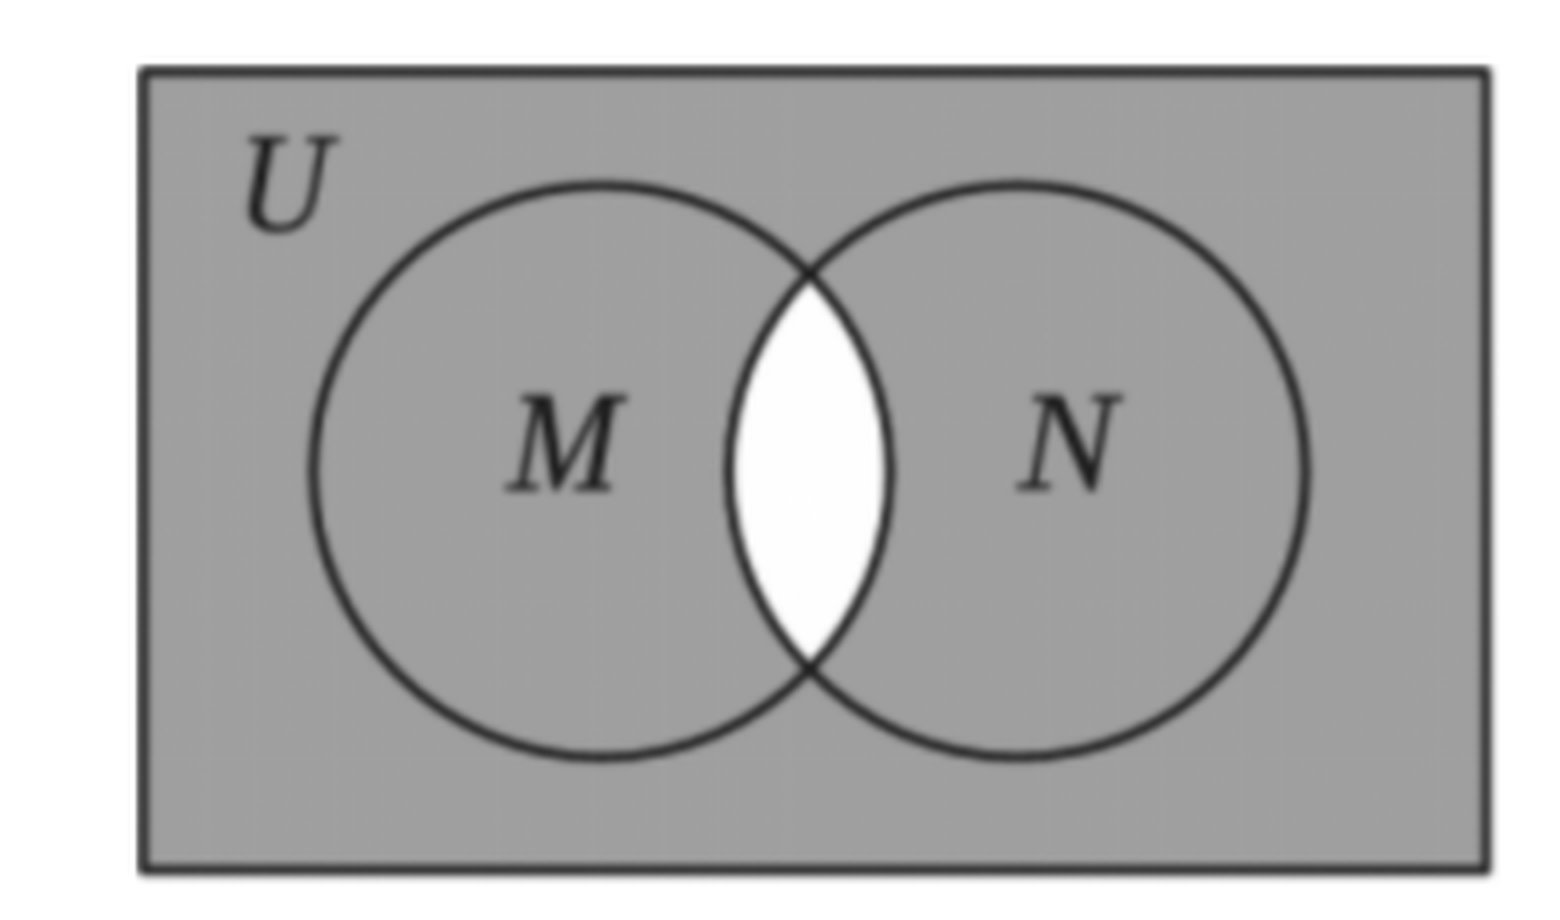
\includegraphics[width=0.40\textwidth]{figures/gao145_q14.png}
\end{center}

\ifanswer
\solbegin
\step{由韦恩图得图中白色区域为集合 $M\cap N$，所以阴影部分表示的集合为 $\overline{M\cap N}$.}
\step{故选 $D$.}
\solend
\fi

% === Q15 ===
\item 已知 $x>-2$，则 $x+\dfrac{1}{x+2}$ 的最小值为\mbox{（\quad）}

\keepwithprev
A. 3\qquad B. 2\qquad C. 1\qquad D. 0

\ifanswer
\solbegin
\step{$x>-2$，则 $x+2>0$，}
\step{所以 $x+\dfrac{1}{x+2}=(x+2)+\dfrac{1}{x+2}-2\geqslant2\sqrt{(x+2)\cdot\dfrac{1}{x+2}}-2=0$，}
\step{当且仅当 $x+2=\dfrac{1}{x+2}$，即 $x=-1$ 时取等号，所以 $x+\dfrac{1}{x+2}$ 的最小值为 $0$.}
\step{故选 $D$.}
\solend
\fi

% 第 16 题：题干在 05 页、解析续至 06 页；两幅数轴标根波浪曲线是【解析】内配图，
% 仅答案版出，放在答案版条件块内 \solbegin 的 \step 之间（照 高一73 第 16 题成例）
\item 关于 $x$ 的不等式 $\dfrac{(x-a)(x-2)^2}{(x-1)(x-5)}\leqslant0$ 的解集中恰有 3 个正整数，则实数 $a$ 的取值范围是\mbox{（\quad）}

\keepwithprev
A. $(-\infty,3]\cup[7,8)$\qquad B. $(-\infty,3)\cup[7,8)$\qquad C. $(-\infty,3]\cup(7,8]$\qquad D. $(-\infty,3)\cup(7,8]$

\ifanswer
\solbegin
\step{由题意，不等式 $\dfrac{(x-a)(x-2)^2}{(x-1)(x-5)}\leqslant0$，}
\step{可化为 $\begin{cases}(x-1)(x-2)^2(x-5)(x-a)\leqslant0\\x\ne1\text{且}x\ne5\end{cases}$，由数轴标根法，}
\step{当 $a=3$ 时，}
\begin{center}
% a=3 数轴标根图取 06 页，去粉色水印、去色、4× LANCZOS 放大；仅答案版出
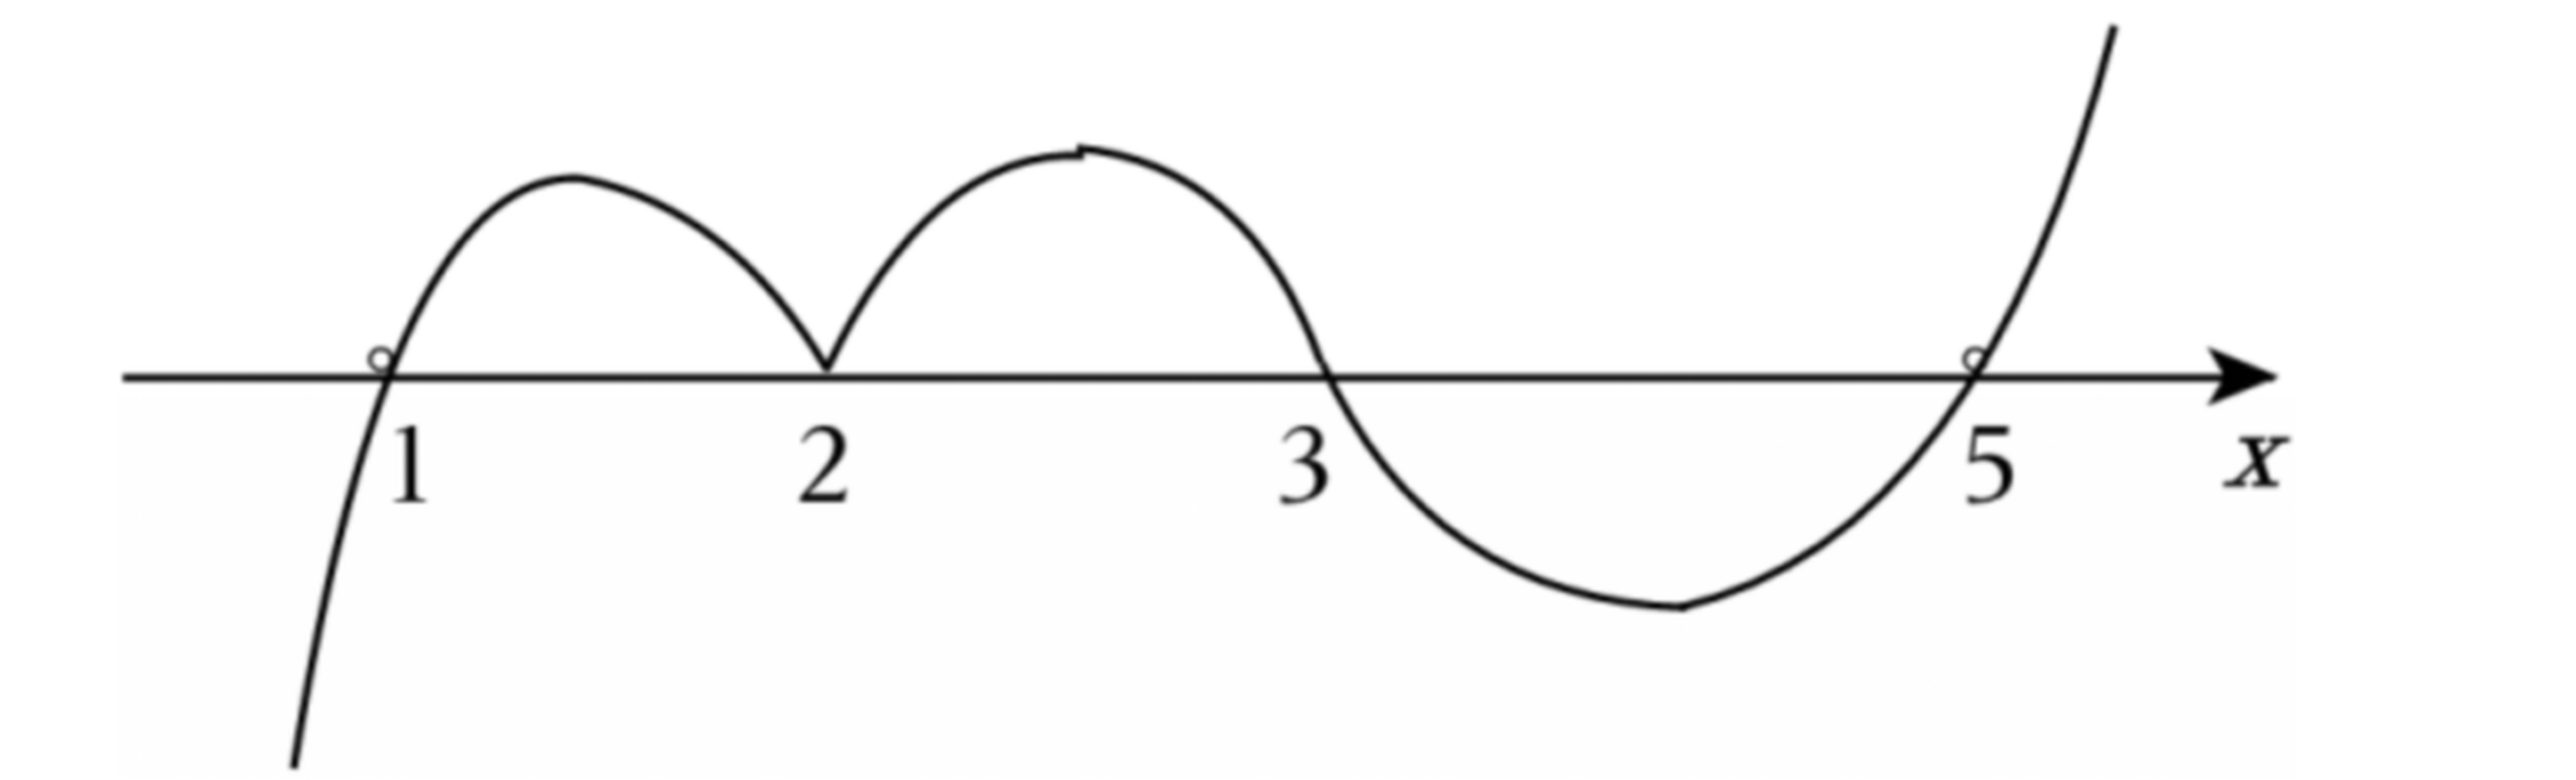
\includegraphics[width=0.62\textwidth]{figures/gao145_q16_a3.png}
\end{center}
\step{得不等式的解集为 $\{x\mid x<1\text{ 或 }x=2\text{ 或 }3\leqslant x<5\}$，}
\step{对应的正整数解为 $2$，$3$，$4$，满足题意，故排除 $B$、$D$；}
\step{当 $a=7$ 时，}
\begin{center}
% a=7 数轴标根图取 06 页，去粉色水印、去色、4× LANCZOS 放大；仅答案版出
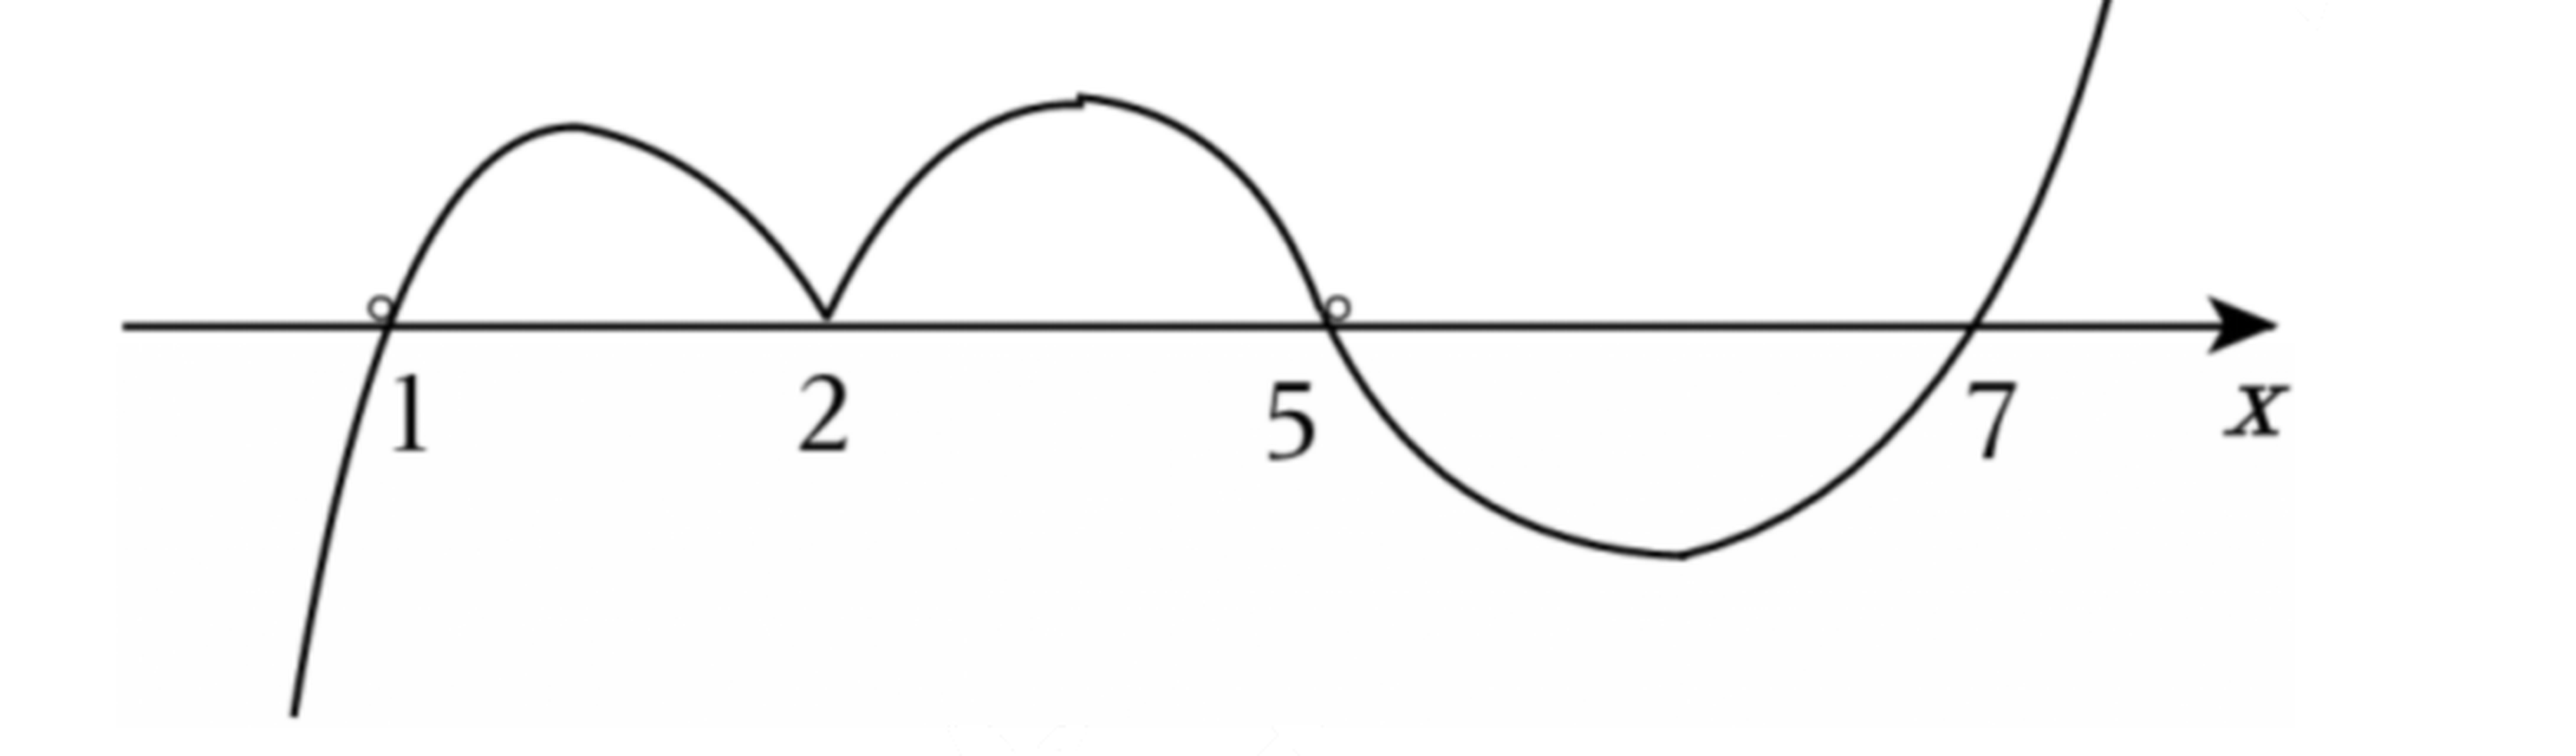
\includegraphics[width=0.62\textwidth]{figures/gao145_q16_a7.png}
\end{center}
\step{得不等式的解集为 $\{x\mid x<1\text{ 或 }x=2\text{ 或 }5<x\leqslant7\}$，}
\step{对应的正整数解为 $2$，$6$，$7$，满足题意，故 $A$ 正确，$C$ 错误.}
\step{故选 $A$.}
\solend
\fi

\end{enumerate}

\bigsec{三、解答题}

\begin{enumerate}
\setcounter{enumi}{16}

% 第 17 题：题干在 06 页、解析续至 07 页，按印刷行断，共 7 行；
% "lg(10÷5)" 的除号照录 \div
\item (1) 已知 $a+a^{-1}=6$，求 $a^2+a^{-2}$ 及 $a^{\frac12}-a^{-\frac12}$ 的值；

(2) 已知 $\lg5=a$，$\lg6=b$，用 $a$、$b$ 分别表示 $\lg2$、$\lg3$、$\lg300$ 和 $\log_{12}15$.

\ifanswer
\solbegin
\step{(1) 因为 $a+a^{-1}=6$，}
\step{所以 $a^2+a^{-2}=(a+a^{-1})^2-2\cdot a\cdot a^{-1}=6^2-2=34$，}
\step{因为 $\left(a^{\frac12}-a^{-\frac12}\right)^2=a-2+a^{-1}=6-2=4$，所以 $a^{\frac12}-a^{-\frac12}=\pm2$；}
\step{(2) $\lg2=\lg(10\div5)=\lg10-\lg5=1-a$，}
\step{$\lg3=\lg(6\div2)=\lg6-\lg2=b-(1-a)=a+b-1$，}
\step{$\lg300=\lg(3\times10^2)=\lg3+\lg10^2=a+b-1+2=a+b+1$，}
\step{所以 $\log_{12}15=\dfrac{\lg15}{\lg12}=\dfrac{\lg3+\lg5}{\lg3+\lg2^2}=\dfrac{a+b-1+a}{a+b-1+2(1-a)}=\dfrac{2a+b-1}{b-a+1}$.}
\solend
\fi

% 第 18 题：题干在 07 页、解析续至 08 页（2 问、分类讨论很长），按印刷行断共 25 行；
% 本卷 Q18 用"图像"（Q13/Q14 用"图象"），逐处照录不统一
\item 已知 $f(x)=(m^2-3m+1)x^{m^2-4m-1}$，$y=f(x)$ 为幂函数且在 $(0,+\infty)$ 上是严格减函数.

(1) 求实数 $m$ 的值以及相应的函数表达式；

(2) 若 $y=f(x)$ 的图像关于 $y$ 轴对称，解关于 $x$ 的不等式 $(x+2)^{1-m}<(3x-1)^{1-m}$.

\ifanswer
\solbegin
\step{(1) 由幂函数的定义得 $m^2-3m+1=1$，}
\step{整理得 $m^2-3m=0$，解得 $m=0$ 或 $m=3$，}
\step{由于 $y=f(x)$ 在 $(0,+\infty)$ 上为严格减函数，}
\step{因此幂函数的指数需满足 $m^2-4m-1<0$，}
\step{当 $m=3$ 时，指数为 $3^2-4\times3-1=-4<0$，满足严格递减条件，}
\step{此时函数表达式为 $f(x)=x^{-4}$，}
\step{当 $m=0$ 时，指数为 $0^2-4\times0-1=-1<0$，满足严格递减条件，}
\step{此时函数表达式为 $f(x)=x^{-1}$，}
\step{所以满足条件的实数 $m$ 为 $0$ 或 $3$，}
\step{对应的函数表达式分别为 $f(x)=x^{-1}$、$f(x)=x^{-4}$；}
\step{(2) 函数图像关于 $y$ 轴对称即函数为偶函数，}
\step{对于 $f(x)=x^{-1}=\dfrac1x$，定义域为 $(-\infty,0)\cup(0,+\infty)$，}
\step{满足 $f(-x)=-f(x)$，为奇函数，图像关于原点对称，}
\step{不满足关于 $y$ 轴对称的条件；}
\step{对于 $f(x)=x^{-4}=\dfrac{1}{x^4}$，定义域为 $(-\infty,0)\cup(0,+\infty)$，}
\step{满足 $f(-x)=f(x)$，为偶函数，图像关于 $y$ 轴对称，}
\step{因此符合条件的 $m$ 值为 $3$，}
\step{将 $m=3$ 代入关于 $x$ 的不等式 $(x+2)^{1-m}<(3x-1)^{1-m}$，}
\step{得 $(x+2)^{1-3}<(3x-1)^{1-3}$，即 $(x+2)^{-2}<(3x-1)^{-2}$，}
\step{因为负指数幂的底数不能为 $0$，所以 $x+2\ne0$ 且 $3x-1\ne0$，}
\step{即 $x\ne-2$ 且 $x\ne\dfrac13$，}
\step{不等式可变形为 $\dfrac{1}{(x+2)^2}<\dfrac{1}{(3x-1)^2}$，}
\step{整理得 $(3x-1)^2<(x+2)^2$，即 $8x^2-10x-3<0$，}
\step{解得 $-\dfrac14<x<\dfrac32$，又 $x\ne-2$ 且 $x\ne\dfrac13$，}
\step{所以不等式的解集为 $\left(-\dfrac14,\dfrac13\right)\cup\left(\dfrac13,\dfrac32\right)$.}
\solend
\fi

% 第 19 题：题干在 08 页、解析续至 09 页，按印刷行断，共 14 行；
% 判别式 cases 块内"△=4a²−16a<0"原卷印扁等边三角 \triangle
%（放大 09 页 zz09_delta.png 与 Q12 高 \Delta 并排确认），逐处照录不统一
\item 已知 $f(x)=ax^2+2ax+4$，$a\in\R$.

(1) 若关于 $x$ 的不等式 $f(x)>0$ 在实数集 $\R$ 上恒成立，求实数 $a$ 的取值范围；

(2) 当 $a<0$ 时，解关于 $x$ 的不等式 $f(x)>(a+1)x+5$.

\ifanswer
\solbegin
\step{(1) 由题意得，关于 $x$ 的不等式 $f(x)>0$ 在实数集 $\R$ 上恒成立，}
\step{即 $ax^2+2ax+4>0$ 在实数集 $\R$ 上恒成立，}
\step{当 $a=0$ 时，不等式为 $4>0$ 恒成立，符合题意；}
\step{当 $a\ne0$ 时，则 $\begin{cases}a>0\\\triangle=4a^2-16a<0\end{cases}$，解得 $0<a<4$.}% 判别式原卷印扁等边三角 $\triangle$，照录
\step{综上所述，实数 $a$ 的取值范围为 $[0,4)$.}
\step{(2) $f(x)=ax^2+2ax+4$，}
\step{当 $a<0$ 时，不等式 $f(x)>(a+1)x+5$ 即为 $ax^2+(a-1)x-1>0$，}
\step{即 $(ax-1)(x+1)>0$，即 $\left(x-\dfrac1a\right)(x+1)<0$，}
\step{当 $a<-1$，即 $\dfrac1a>-1$ 时，解得 $-1<x<\dfrac1a$；}
\step{当 $a=-1$，即 $\dfrac1a=-1$ 时，解得 $x\in\varnothing$；}
\step{当 $-1<a<0$，即 $\dfrac1a<-1$ 时，解得 $\dfrac1a<x<-1$.}
\step{综上所述，当 $a<-1$ 时，不等式的解集为 $\left\{x\mid -1<x<\dfrac1a\right\}$；}
\step{当 $a=-1$ 时，不等式的解集为 $\varnothing$；}
\step{当 $-1<a<0$ 时，不等式的解集为 $\left\{x\mid \dfrac1a<x<-1\right\}$.}
\solend
\fi

% 第 20 题：菜园靠墙图为题目配图（三版都出），题干写"如图"；
% 题干在 09 页（含图）、解析续至 10 页，按印刷行断，共 13 行
\needvspace{8cm}
\item 如图，某人计划用篱笆围成一个一边靠墙（墙足够长）的矩形菜园. 设菜园的长为 $x$ 米，宽为 $y$ 米.

\begin{center}
% 矩形菜园靠墙图取 09 页右下，去粉色水印、去色、4× LANCZOS 放大
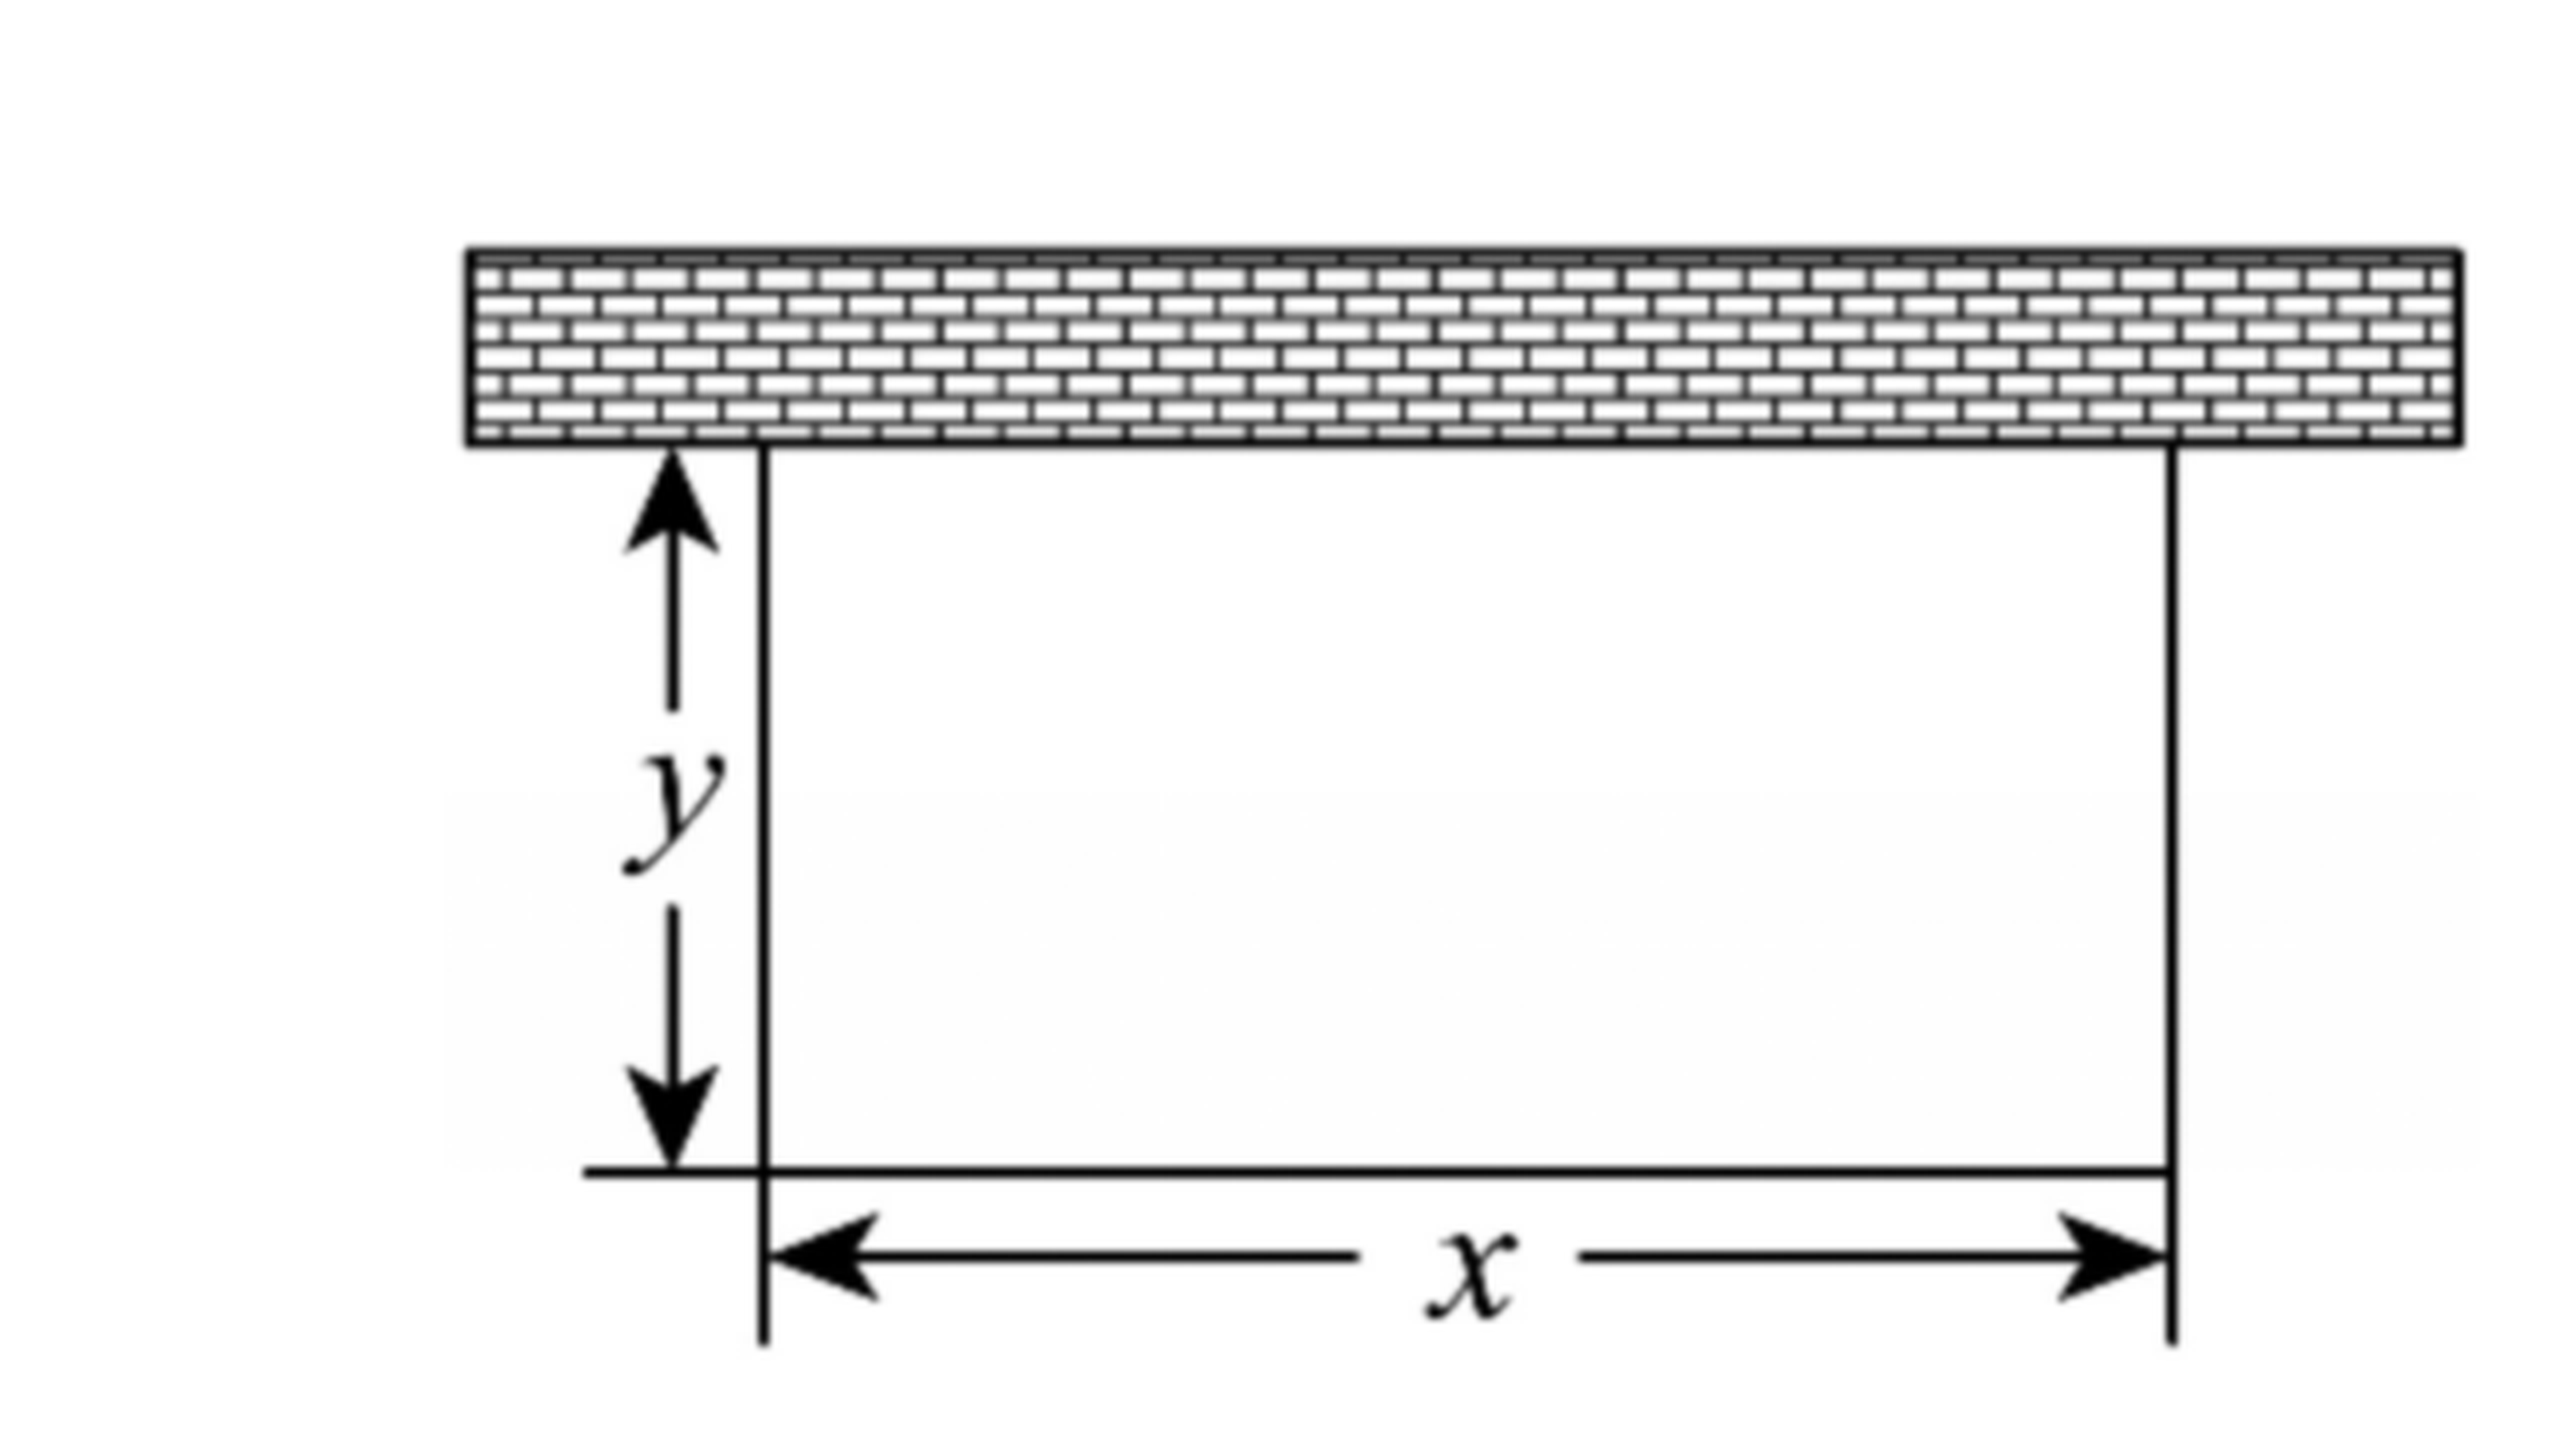
\includegraphics[width=0.55\textwidth]{figures/gao145_q20.png}
\end{center}

(1) 若菜园面积为 72 平方米，则 $x$、$y$ 为何值时，所用篱笆总长最小？

(2) 若 $x$、$y$ 满足 $x+y-xy+63=0$，则菜园面积最小为多少平方米？

\ifanswer
\solbegin
\step{(1) 由题意得，菜园的面积 $S=xy=72$，且 $x>0$，$y>0$，}
\step{所用篱笆总长 $L=x+2y$，}
\step{由基本不等式得 $x+2y\geqslant2\sqrt{x\cdot2y}=2\sqrt{2xy}=2\sqrt{2\times72}=24$，}
\step{当且仅当 $x=2y$ 时取等号，}
\step{联立 $\begin{cases}xy=72\\x=2y\end{cases}$，解得 $\begin{cases}x=12\\y=6\end{cases}$，}
\step{所以当 $x=12$，$y=6$ 时，所用篱笆总长最小；}
\step{(2) 由题意得 $x>0$，$y>0$，且满足 $x+y-xy+63=0$，即 $x+y=xy-63$，}
\step{由基本不等式得 $x+y\geqslant2\sqrt{xy}$，当且仅当 $x=y$ 时取等号，}
\step{所以 $xy-63\geqslant2\sqrt{xy}$. 令 $t=\sqrt{xy}(t>0)$，则 $xy=t^2$，}
\step{上述不等式可化为 $t^2-2t-63\geqslant0$，即 $(t-9)(t+7)\geqslant0$，}
\step{因为 $t>0$，所以 $t+7>0$，故 $t-9\geqslant0$，解得 $t\geqslant9$，所以 $\sqrt{xy}\geqslant9$，}
\step{即 $xy\geqslant81$，当且仅当 $x=y=9$ 时取等号，此时满足 $9+9-81+63=0$，}
\step{所以菜园面积最小为 81 平方米.}
\solend
\fi

% 第 21 题：题干在 10 页、解析续至 11 页（3 问、分类讨论很长），按印刷行断共 22 行；
% 末行"故第 2026 个元素是 2700 之后第一个属于 A 的数，即 2701." 为全卷收尾，
% 无 Q22/Q23、无附加题节；数集 Z/N* 按全稿惯例改 \Z/\N^*
\item 已知集合 $A=\{x\mid x=m^2-n^2$，$m$、$n\in\Z\}$.

(1) 求证：任何奇数 $2k+1(k\in\Z)$ 都是集合 $A$ 中的元素；

(2) 判断偶数 $4k-2(k\in\Z)$ 是否为集合 $A$ 的元素？请说明理由；

(3) 若将集合 $A$ 中的正整数由小到大排列，求出集合 $A$ 中第 2026 个正整数.

\ifanswer
\solbegin
\step{(1) 因为 $x=(k+1)^2-k^2=2k+1(k\in\Z)$，}
\step{所以任何奇数 $2k+1(k\in\Z)$ 都属于集合 $A$；}
\step{(2) 偶数 $4k-2(k\in\Z)$ 不是集合 $A$ 的元素，理由如下：}
\step{由题意得 $x=m^2-n^2=(m-n)(m+n)$，}
\step{当 $m$、$n$ 均为奇数时，设 $m=2k_1+1$，$n=2k_2+1(k_1$、$k_2\in\Z)$，}
\step{则 $m^2-n^2=(2k_1+1)^2-(2k_2+1)^2=(2k_1-2k_2)(2k_1+2k_2+2)$}
\step{$=4(k_1-k_2)(k_1+k_2+1)$，}
\step{因为 $k_1$、$k_2\in\Z$，所以 $k_1-k_2\in\Z$，$k_1+k_2+1\in\Z$，}
\step{从而 $m^2-n^2$ 为 $4$ 的倍数；}
\step{当 $m$、$n$ 均为偶数时，设 $m=2k_1$，$n=2k_2(k_1$、$k_2\in\Z)$，}
\step{$m^2-n^2=4k_1^2-4k_2^2=4(k_1^2-k_2^2)$ 为 $4$ 的倍数；}
\step{当 $m$、$n$ 为一个偶数一个奇数时，不妨设 $m$ 为偶数，$n$ 为奇数，}
\step{设 $m=2k_1$，$n=2k_2+1(k_1$、$k_2\in\Z)$，}
\step{则 $m^2-n^2=4k_1^2-(2k_2+1)^2=4(k_1^2-k_2^2-k_2)-1$ 为奇数.}
\step{无论哪种情况均不满足 $4k-2(k\in\Z)$，}
\step{故偶数 $4k-2(k\in\Z)$ 不是集合 $A$ 的元素；}
\step{(3) 由前两问得，$4$ 的倍数和奇数属于集合 $A$ 中的元素，}
\step{令集合 $A$ 中的正整数元素为 $4k-3$、$4k-1$、$4k(k\in\N^*)$，}
\step{对任意的 $k\in\N^*$，连续的 $4$ 个整数 $4k-3$、$4k-2$、$4k-1$、$4k$ 中}
\step{有三个数 $4k-3$、$4k-1$、$4k$ 都在集合 $A$ 中，}
\step{因为 $2026=3\times675+1$，所以集合 $A$ 中第 $2025$ 个元素为 $4\times675=2700$，}
\step{故第 2026 个元素是 2700 之后第一个属于 $A$ 的数，即 2701.}
\solend
\fi

\end{enumerate}

\end{document}
"
%
% ① 原始材料：微信公众号"魔都数学加油站"文章，连载"27学年高一145"，原文标题
% "27学年高一145——2026-2027年上海市市二中学高一上期中"；
% 原文链接：https://mp.weixin.qq.com/s/6V-i9KE0GWodC-wmd5z8nQ 。
% 正文为 11 张 PNG 页（01/02/03/08/10/11 为 4762×6735，04/05/06/07/09 为 2560×3620，
% 同一篇各页分辨率不同，逐页按各自分辨率裁图核对，别按预览比例换算裁框）。
% 题目下印【答案】或【解析】，为混合体例讲评版：Q3 只印【答案】、无【解析】，其余
% 18 题印【解析】。题目、解析均据原图转录；卷面粉红色水印"魔都数学加油站"及
% 公众号页脚未录入。
% 全卷插图情况（逐页通读 11 页确认，题干写"如图"处均配有图）：
%   · Q14 韦恩图（05 页右侧，全集 U 矩形＋两圆 M/N＋白色交集、灰色阴影＋U/M/N 标注）：
%     题目配图（选择题选项旁），三版都出，裁自 05 页去水印去色 4× 放大存
%     figures/gao145_q14.png；
%   · Q16 两幅数轴标根波浪曲线（06 页，a=3 与 a=7 各一幅，标根法画
%     (x-1)(x-2)^2(x-5)(x-a)≤0 的符号曲线）：【解析】内的配图，仅答案版出，
%     裁 figures/gao145_q16_a3.png / figures/gao145_q16_a7.png（或合并一张），
%     放在答案版条件块内 \solbegin 的 \step 之间（照 高一73 第 16 题成例）；
%   · Q20 矩形菜园靠墙图（09 页右下，灰色砖墙＋矩形菜园＋x/y 标注＋箭头）：
%     题目配图，三版都出，裁自 09 页去水印去色 4× 放大存 figures/gao145_q20.png；
%   其余各页逐页确认无其它题目配图、无表格、亦无"题干写如图而源码漏图"一处。
%
% 卷首标题：原卷印作"2026-2027 年市二中学高一上期中"，年份区间按全稿惯例排 en dash；
% 原卷卷面未印副标题，本稿按同期中卷（高一140／141／143／144）知识模块口径补出
% "集合与常用逻辑用语、不等式、函数"。
%
% 题号体例：本卷共 19 题——一、填空题 3—12（10 题）、二、选择题 13—16（4 题）、
% 三、解答题 17—21（5 题）。三节分别 \setcounter{enumi}{2}／{12}／{16}。
% 原卷从第 3 题起、无第 1、2 题，本稿保留原题号；全卷无附加题节。
%
% ② 与原卷的排版差异：
%   ① 原文从第 3 题起，本稿保留原题号；共 19 题三节；
%   ② 混合体例：原卷 Q3 只印【答案】、无【解析】（"第一步应假设___。
%      【答案】x≤2 或 y≤2"），按 高一140 第 5 题成例提 \ans{}、不补造解析；
%      其余 18 题印【解析】，用 \solbegin…\solend，选择题答案在解析末句"故选 X"
%      （Q13 选 B、Q14 选 D、Q15 选 D、Q16 选 A，逐个放大原图核实）、
%      题干括号 \mbox{（\quad）} 留空、不另提 \ans{}；填空／解答答案落在解析里；
%      答案版【答案】/【解析】标记数 = 19（1 个 \ans ＋ 18 个 \solbegin）= 全卷题数；
%   ③ 原卷卷面未印副标题，本稿按知识模块口径补出；
%   ④ 原卷填空横线按全稿惯例排 \blankline[4.4em]；选择题括号排 \mbox{（\quad）}、
%      选项段前按惯例加 \keepwithprev；解答题不留作答区、不加 \anspace
%      （原卷为讲评版，与 129／131／132／133／136／140／141／143／144 同）；
%   ⑤ 数集：Q9"a、b∈R"、Q12"a∈R"、Q21"m、n∈Z""k∈Z""k∈N*"等原卷印
%      斜体或黑板粗体 R/Z/N，按全稿惯例统一改 \R／\Z／\N^*；绝对值排 \lvert…\rvert，
%      集合描述竖线排 \mid；不等号按全稿惯例排 \leqslant／\geqslant；
%      补集照原卷上划线排 \overline{M}／\overline{N}（Q14 选项 B/C/D 逐处核）；
%      空集记号 \varnothing；\subset（单线⊂）与 \subseteq（带下划线⊆）逐处照录不统一；
%   ⑥ 子题标号 (1)(2)(3) 原卷印半角括号照录；圈数字进数学式用 \text{①}（否则 FONTCHK 挂）；
%      \left…\right 不得拆到不同 $…$ 组；cases 块整体算一个印刷行；
%   ⑦ 题干／解析中的中文弯引号按原卷照录（Q3"若 x+y>4，则 x>2 且 y>2"、
%      Q11"a₁/a₂=b₁/b₂""M=N"、选填"充分非必要""必要非充分""充要""既非充分也非必要"
%      等，含引号内空格），注释内一律 ASCII 引号；数学式内 CJK 用 \text{}；
%   ⑧ 半角逗号在数学组之间是全稿惯例、非笔误（如 Q5"x₁+x₂=6，x₁x₂=√3"、
%      Q7"a>1，b>1"、指数／对数式内逗号），逐处照录别改全角；行末西文句点照录为
%      ASCII `.`；行中全角逗号／顿号照录；
%   ⑨ "图像／图象"逐处照录不统一（Q18"图像关于 y 轴对称"等，核全卷）；
%   ⑩ 判别式 Δ/△ 混用是照录项：Q12 解析"Δ=a²−4a²(2a−3)>0"、
%      Q19 解析"Δ=4a²−16a<0"等，放大原图判断是高 \Delta（等腰偏高、高>宽）
%      还是扁 \triangle，逐处照录不得统一（参照 高一142／144 头注④口径）；
%   ⑪ 一条 \step = 原卷解析的一个印刷行，cases 块整体算一个印刷行；别把原卷折行
%      并起来、别把一行拆多条。Q6 分段讨论、Q12 三个 cases 条件组、Q16 数轴标根、
%      Q18／Q19 分类讨论、Q21 三问均按印刷行逐条断，不丢行；
%   ⑫ Q14 韦恩图为"题干＋选项＋图"整块，加 \needvspace 守卫推走（守卫放 \item 之前，
%      见 高一140 Q14、高一144 Q17 成例与切页审计 B 类坑）；Q20 菜园图同理；
%      三版切页审计均"合计异常：无"；
%   ⑬ 跨页续印按题合并：Q3/4/5/6 在 01 页（Q6 解析续 02 页顶）；Q7/8/9/10 在 02 页
%      （Q10 解析续 03 页）；Q11/12 在 03 页（Q12 解析续 04 页，很长）；
%      Q13 在 04 页末、解析在 05 页顶；Q14/15/16 在 05 页（Q16 解析续 06 页含两幅数轴图）；
%      Q17 在 06 页、解析续 07 页；Q18 在 07 页、解析续 08 页；Q19 在 08 页、解析续 09 页；
%      Q20 在 09 页（含菜园图）、解析续 10 页；Q21 在 10 页、解析续 11 页
%      （末页收尾"故第 2026 个元素是 2700 之后第一个属于 A 的数，即 2701."、
%      无 Q22/Q23、无附加题节）。本稿按题连排，不丢行、不并折行；
%   ⑭ 原卷解析内若有红色"法一／法二"之类小标题，按全稿惯例排 \stepm{标签}{…}
%      （黑体着色、不引入红色、不改 common.sty），头注注明；水印"魔都数学加油站"
%      红色不录入。
%
% ③ 行数复核：一条 \step／\stepm = 原卷解析的一个印刷行，cases 块作一个印刷行计。
%   逐题数（主会话逐页核对定稿）：Q3：0（只印【答案】、提 \ans{}，不计入 \step 账）；
%   Q4：3；Q5：2；Q6：10；Q7：3；Q8：3；Q9：2；Q10：7；Q11：4；Q12：12；
%   Q13：2；Q14：2；Q15：4；Q16：9；Q17：7；Q18：25；Q19：14；Q20：13；Q21：22。
%   合计 144 条 \step（本卷无 \stepm：解析内无红色"法一／法二"类小标题），
%   与原卷逐题印刷行相等。全卷 18 题设 \solbegin…\solend ＋ Q3 一处 \ans{}，
%   答案版【答案】/【解析】标记数 = 19 = 全卷题数。
%
% ④ 判别式／子集符号结论（逐处放大原图照录、不得统一，主会话像素级复核）：
%   判别式全卷 2 处、两形混用逐处照录不统一（参照 高一142／144 头注④口径）：
%     · Q12 解析 cases 块"Δ=a²−4a²(2a−3)>0" 原卷印等腰偏高粗三角（高>宽），
%       照录 \Delta（放大 04 页 /tmp/gao145s2/main_q12_delta.png 确认）；
%     · Q19 解析 cases 块"△=4a²−16a<0" 原卷印扁等边空心三角（宽≈高、细线），
%       照录 \triangle（放大 09 页 /tmp/gao145s2/main_q19_delta.png 确认）。
%   子集／补集：Q14 选项 A `M\cup N`、B `M\cap\overline{N}`（上划线只在 N 上）、
%   C `\overline{M\cup N}`（罩整个 M∪N）、D `\overline{M\cap N}`（罩整个 M∩N，
%   非 \overline{M}\cap N；放大 05 页 /tmp/gao145s2/main_q14_opts.png 确认），
%   阴影为灰色区域＝全集减白色交集，答案 D，照录 \overline{M\cap N}；
%   全集卷无 \subset／\subseteq 混用（本卷集合题用 \cup／\cap／\overline{}）；
%   空集 \varnothing（Q19 解析 x∈\varnothing）；数集 \R／\Z／\N^* 归一见 ② ⑤。
%
% ⑤ 存疑照录（放大原图确认，照录未改、正文对应处另有 % 注）：
%   1. Q3 题干"若 x+y>4，则 x>2 且 y>2" 后"时"前留一空格、弯引号内空格照录；
%      该卷混合体例（Q3 只印【答案】、提 \ans{}）见 ② ②。
%   2. Q4／Q5 解析中的"1，3，5 和 6"、"x₁+x₂=6,x₁x₂=√3" 等半角／全角逗号
%      逐处照原卷（放大 01 页确认），数学式内半角逗号为全稿惯例、非笔误。
%   3. Q14 选项 D 上划线罩住整个 M∩N（而非仅罩 M），照录 \overline{M\cap N}。
%   4. Q12 判别式高 \Delta 与 Q19 判别式扁 \triangle 两形混用，逐处照录不统一（见 ④）。
%   全卷除此 4 类外未发现其它笔误／自相矛盾处。
%
% ⑥ 跨页续印按题合并说明：见 ② ⑬。
%
\documentclass[a4paper,11pt]{article}
\usepackage{common}

\begin{document}

\examtitlest[3]{2026--2027 年市二中学高一上期中}{集合与常用逻辑用语、不等式、函数}

\bigsec{一、填空题}

\begin{enumerate}
\setcounter{enumi}{2}

% 第 3 题：原卷只印【答案】、无【解析】（放大 01 页确认），按 高一140 第 5 题成例
% 提 \ans{}、不补造解析；题干中文弯引号与"时"前空格照录
\item 用反证法证明命题：“若 $x+y>4$，则 $x>2$ 且 $y>2$” 时，第一步应假设\blankline[4.4em].

\ifanswer
\ans{$x\leqslant2$ 或 $y\leqslant2$}
\fi

% === Q4 ===
\item 设集合 $M$ 满足 $\{1,3,5,6\}\cup M=\{1,2,3,4,5,6\}$，则满足条件的所有 $M$ 的个数为\blankline[4.4em].

\ifanswer
\solbegin
\step{集合 $M$ 满足 $\{1,3,5,6\}\cup M=\{1,2,3,4,5,6\}$，}
\step{则 $M$ 中必含有 $2$ 和 $4$，$1$，$3$，$5$ 和 $6$ 可以选也可不选，}
\step{则满足条件的所有 $M$ 的数目相当于集合 $\{1,3,5,6\}$ 的子集的个数 $2^4=16$.}
\solend
\fi

% === Q5 ===
\item 已知方程 $x^2-6x+\sqrt3=0$ 的两根为 $x_1$ 和 $x_2$，则 $(x_1-x_2)^2=$\blankline[4.4em].

\ifanswer
\solbegin
\step{因为方程 $x^2-6x+\sqrt3=0$ 的两根为 $x_1$ 和 $x_2$，所以 $x_1+x_2=6,x_1x_2=\sqrt3$，}% 数学式内半角逗号为全稿惯例，照录
\step{所以 $(x_1-x_2)^2=(x_1+x_2)^2-4x_1x_2=36-4\sqrt3$.}
\solend
\fi

% 第 6 题：题干在 01 页，解析续至 02 页顶（末 2 行），按印刷行逐条断，共 10 行
\item 不等式 $\lvert x-2026\rvert+\lvert x-2029\rvert>3$ 的解集是\blankline[4.4em].

\ifanswer
\solbegin
\step{当 $x<2026$ 时，$x-2026<0$，$x-2029<0$，}
\step{原不等式可化为 $(2026-x)+(2029-x)>3$，解得 $x<2026$，}
\step{故此时，不等式的解为 $x<2026$；}
\step{当 $2026\leqslant x\leqslant2029$ 时，$x-2026\geqslant0$，$x-2029\leqslant0$，}
\step{原不等式可化为 $(x-2026)+(2029-x)>3$，即 $3>3$，显然不成立，}
\step{故此时，不等式无解；}
\step{当 $x>2029$ 时，$x-2026>0$，$x-2029>0$，}
\step{原不等式可化为 $(x-2026)+(x-2029)>3$，解得 $x>2029$，}
\step{故此时，不等式的解为 $x>2029$.}
\step{综上，原不等式的解集为 $(-\infty,2026)\cup(2029,+\infty)$.}
\solend
\fi

% === Q7 ===
\item 已知 $a>1$，$b>1$，若 $\log_a b+\log_b a=2$，且 $ab=2$，则 $\log_2(a+b)=$\blankline[4.4em].

\ifanswer
\solbegin
\step{由 $\log_a b+\log_b a=2$，$a>1$，$b>1$，得 $\log_a b+\dfrac{1}{\log_a b}=2$，}
\step{即 $(\log_a b)^2-2\log_a b+1=0$，则 $(\log_a b-1)^2=0$，解得 $\log_a b=1$，即 $a=b$，}
\step{又 $ab=2$，所以 $a=b=\sqrt2$，所以 $\log_2(a+b)=\log_2 2\sqrt2=\log_2 2^{\frac32}=\dfrac32$.}
\solend
\fi

% === Q8 ===
\item 已知 $m>0$，$n>0$，且 $m+n=1$，则 $\dfrac1m+\dfrac4n$ 的最小值为\blankline[4.4em].

\ifanswer
\solbegin
\step{由 $m>0$，$n>0$，$m+n=1$，}
\step{则 $\dfrac1m+\dfrac4n=(m+n)\left(\dfrac1m+\dfrac4n\right)=5+\dfrac nm+\dfrac{4m}n\geqslant5+2\sqrt{\dfrac nm\cdot\dfrac{4m}n}=9$，}
\step{当且仅当 $n=2m=\dfrac23$ 时，上式取得等号，故最小值为 $9$.}
\solend
\fi

% === Q9 ===
\item 已知 $a$、$b\in\R$，且 $3a+2b=1$，则 $8^a+4^b$ 最小值为\blankline[4.4em].

\ifanswer
\solbegin
\step{因为 $3a+2b=1$，所以 $8^a+4^b=2^{3a}+2^{2b}\geqslant2\sqrt{2^{3a+2b}}=2\sqrt2$，}
\step{当且仅当 $3a=2b$ 时取等号，故最小值为 $2\sqrt2$.}
\solend
\fi

% 第 10 题：题干在 02 页、解析续至 03 页顶，按印刷行断，共 7 行
\item 已知关于 $x$ 的不等式 $ax^2+bx+c>0$ 的解集为 $\{x\mid 1<x<2\}$，则关于 $x$ 的不等式 $bx^2-ax+c<0$ 的解集为\blankline[4.4em].

\ifanswer
\solbegin
\step{已知关于 $x$ 的不等式 $ax^2+bx+c>0$ 的解集为 $\{x\mid 1<x<2\}$，}
\step{由解集为 $1<x<2$ 且二次函数在两根之间为正，得 $a<0$，两个根为 $1$，$2$，}
\step{所以 $ax^2+bx+c=a(x-1)(x-2)=ax^2-3ax+2a$，}
\step{比较系数得 $b=-3a$，$c=2a$.}
\step{于是 $bx^2-ax+c=-3ax^2-ax+2a=-a(3x-2)(x+1)$，}
\step{$a<0$，故 $bx^2-ax+c<0$ 等价于 $(3x-2)(x+1)<0$，解得 $-1<x<\dfrac23$，}
\step{故 $bx^2-ax+c<0$ 的解集为 $\left\{x\mid -1<x<\dfrac23\right\}$.}
\solend
\fi

% 第 11 题：题干引号内空格照录（放大 03 页确认），四组选填引号亦同；
% 结论"故为必要非充分条件"照录，解析共 4 个印刷行
\item 设 $a_1$、$b_1$、$a_2$、$b_2$ 均为非零实数，不等式 $a_1x+b_1>0$ 和 $a_2x+b_2>0$ 的解集分别为集合 $M$、$N$，那么 “ $\dfrac{a_1}{a_2}=\dfrac{b_1}{b_2}$ ” 是 “ $M=N$ ” 的\blankline[4.4em]条件（选填 “ 充分非必要 ”、“ 必要非充分 ”、“ 充要 ” 和 “ 既非充分也非必要 ”）.

\ifanswer
\solbegin
\step{当 $a_1=b_1=1$，$a_2=b_2=-1$ 时，满足 $\dfrac{a_1}{a_2}=\dfrac{b_1}{b_2}$，}
\step{但是 $M=N$ 不成立，即充分性不成立；}
\step{若 $M=N$ 时，$\dfrac{a_1}{a_2}=\dfrac{b_1}{b_2}$ 一定成立，即必要性成立.}
\step{故为必要非充分条件.}
\solend
\fi

% 第 12 题：题干在 03 页、解析续至 04 页（很长，含 3 个 cases 条件组），
% 按印刷行逐条断共 12 行；cases 块整体算一个印刷行
\item 已知 $f(x)=\dfrac{ax+3}{x-2}$（常数 $a\in\R$）. 函数 $y=f(x)$ 在区间 $[3,+\infty)$ 上是严格减函数，且函数值不恒为负. 若关于 $x$ 的方程 $f(x)=\dfrac{a}{ax-1}$ 有两个不相等的实数根 $x_1$ 和 $x_2$，则 $a$ 的取值范围是\blankline[4.4em].

\ifanswer
\solbegin
\step{$f(x)=\dfrac{ax+3}{x-2}=a+\dfrac{3+2a}{x-2}$，定义域 $(-\infty,2)\cup(2,+\infty)$，}
\step{由于 $y=f(x)$ 在区间 $[3,+\infty)$ 上是严格减函数，且函数值不恒为负，}
\step{所以 $\begin{cases}3+2a>0\\a+\dfrac{3+2a}{3-2}\geqslant0\end{cases}\Rightarrow a\geqslant-1$，}
\step{若关于 $x$ 的方程 $f(x)=\dfrac{a}{ax-1}$ 有两个不相等的实数根 $x_1$ 和 $x_2$，}
\step{则 $\dfrac{ax+3}{x-2}=\dfrac{a}{ax-1}$，即 $(ax+3)(ax-1)=a(x-2)$，$x\ne2$ 且 $ax-1\ne0$，}
\step{当 $a\ne0$ 且 $a\geqslant-1$ 时，$(ax+3)(ax-1)=a(x-2)$，$x\ne2$ 且 $ax-1\ne0$，}
\step{可化为 $\begin{cases}a^2x^2+ax+2a-3=0\\x\ne2,x\ne\dfrac1a\end{cases}$，}
\step{要使方程有两个不相等的实数根 $x_1$ 和 $x_2$，}
\step{则 $\begin{cases}\Delta=a^2-4a^2(2a-3)>0\\a\geqslant-1\text{且}a\ne0\\4a^2+2a+2a-3\ne0\\a^2\cdot\dfrac1{a^2}+a\cdot\dfrac1a+2a-3\ne0\end{cases}\Rightarrow\begin{cases}a<\dfrac{13}{8}\\a\geqslant-1\text{且}a\ne0\\a\ne\dfrac12\text{且}a\ne-\dfrac32\\a\ne\dfrac12\end{cases}$，}% 判别式原卷印等腰偏高三角 $\Delta$，照录（放大 04 页 zz04_delta.png 确认）
\step{得 $-1\leqslant a<\dfrac{13}{8}$ 且 $a\ne0,a\ne\dfrac12$；}
\step{当 $a=0$ 时，方程无解；}
\step{所以 $a$ 的取值范围是 $[-1,0)\cup\left(0,\dfrac12\right)\cup\left(\dfrac12,\dfrac{13}{8}\right)$.}
\solend
\fi

\end{enumerate}

\bigsec{二、选择题}

\begin{enumerate}
\setcounter{enumi}{12}

% 第 13 题：题干在 04 页末、解析在 05 页顶；"图象"照录（本卷 Q13、Q14 用"图象"）
\item 已知幂函数 $f(x)$ 的图象过点 $\left(7,\dfrac{1}{\sqrt7}\right)$，则 $f(x)=$\mbox{（\quad）}

\keepwithprev
A. $x^{-2}$\qquad B. $x^{-\frac12}$\qquad C. $x^{\frac12}$\qquad D. $x^2$

\ifanswer
\solbegin
\step{设幂函数 $f(x)=x^\alpha(\alpha\in\R)$，因为幂函数的图象过点 $\left(7,\dfrac{1}{\sqrt7}\right)$，}
\step{所以 $7^\alpha=\dfrac{1}{\sqrt7}=7^{-\frac12}$，所以 $\alpha=-\dfrac12$，故 $f(x)=x^{-\frac12}$. 故选 $B$.}
\solend
\fi

% 第 14 题：韦恩图为题目配图（三版都出），"题干＋选项＋图"整块，needvspace
% 守卫放在 \item 之前（Q14 为选择题节内第二题，不会让节标题孤落页末）；
% D 选项上划线罩住整个 M∩N（放大 05 页 zz05_q14D.png 确认，非 \overline{M}\cap N）
\needvspace{9cm}
\item 已知全集 $U$ 和集合 $M$、$N$，用集合语言表示图中的阴影部分，正确的是\mbox{（\quad）}

\keepwithprev
A. $M\cup N$\qquad B. $M\cap\overline{N}$\qquad C. $\overline{M\cup N}$\qquad D. $\overline{M\cap N}$

\begin{center}
% 韦恩图取 05 页右侧，去粉色水印、去色、4× LANCZOS 放大
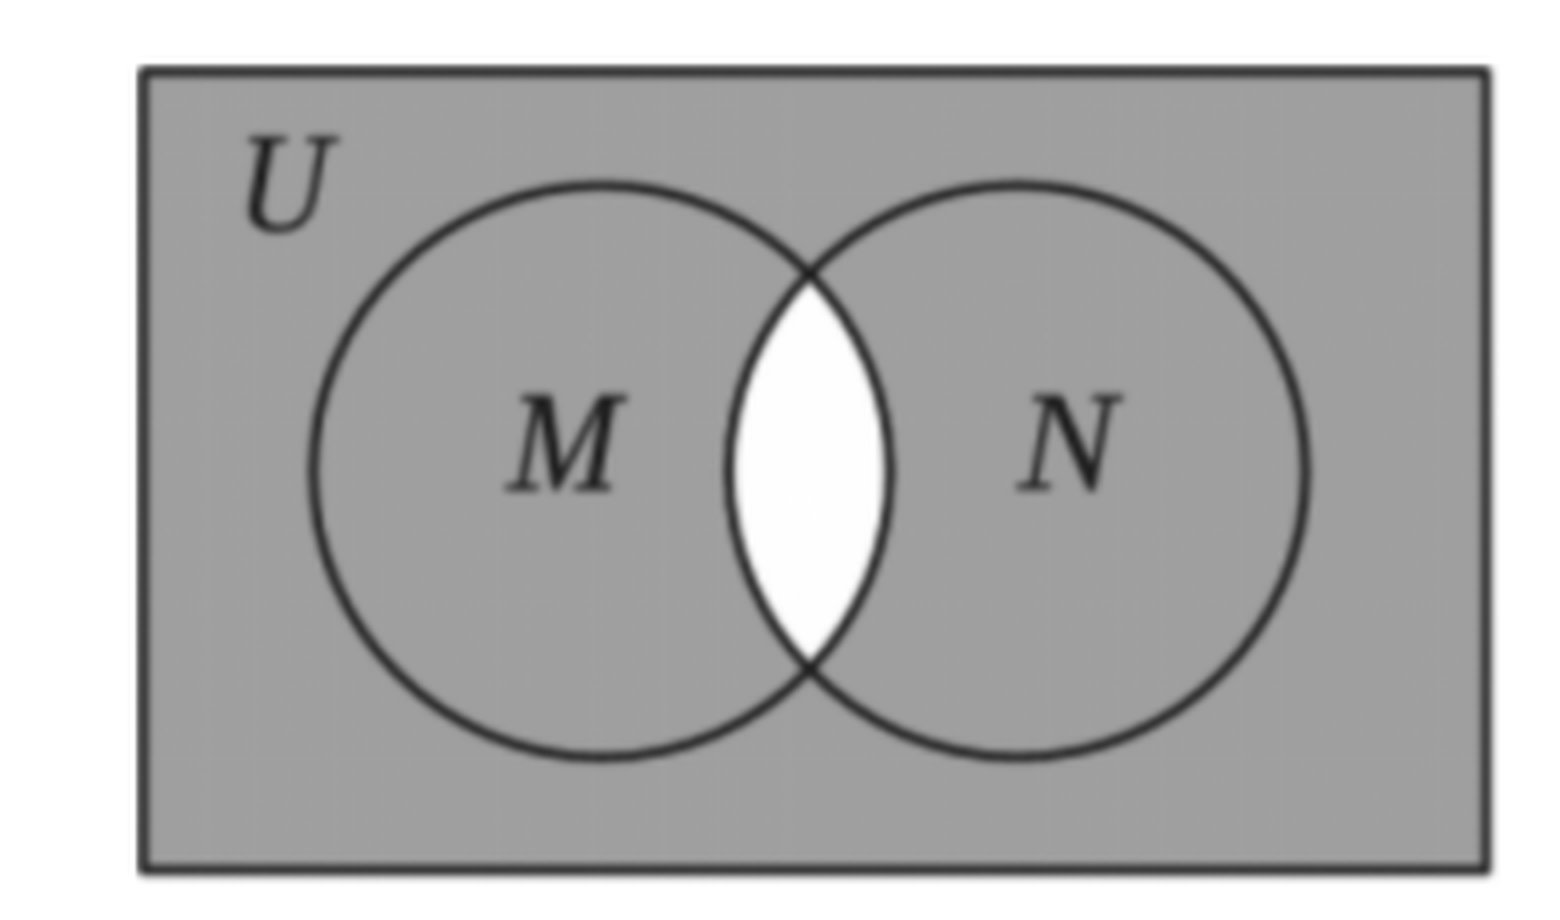
\includegraphics[width=0.40\textwidth]{figures/gao145_q14.png}
\end{center}

\ifanswer
\solbegin
\step{由韦恩图得图中白色区域为集合 $M\cap N$，所以阴影部分表示的集合为 $\overline{M\cap N}$.}
\step{故选 $D$.}
\solend
\fi

% === Q15 ===
\item 已知 $x>-2$，则 $x+\dfrac{1}{x+2}$ 的最小值为\mbox{（\quad）}

\keepwithprev
A. 3\qquad B. 2\qquad C. 1\qquad D. 0

\ifanswer
\solbegin
\step{$x>-2$，则 $x+2>0$，}
\step{所以 $x+\dfrac{1}{x+2}=(x+2)+\dfrac{1}{x+2}-2\geqslant2\sqrt{(x+2)\cdot\dfrac{1}{x+2}}-2=0$，}
\step{当且仅当 $x+2=\dfrac{1}{x+2}$，即 $x=-1$ 时取等号，所以 $x+\dfrac{1}{x+2}$ 的最小值为 $0$.}
\step{故选 $D$.}
\solend
\fi

% 第 16 题：题干在 05 页、解析续至 06 页；两幅数轴标根波浪曲线是【解析】内配图，
% 仅答案版出，放在答案版条件块内 \solbegin 的 \step 之间（照 高一73 第 16 题成例）
\item 关于 $x$ 的不等式 $\dfrac{(x-a)(x-2)^2}{(x-1)(x-5)}\leqslant0$ 的解集中恰有 3 个正整数，则实数 $a$ 的取值范围是\mbox{（\quad）}

\keepwithprev
A. $(-\infty,3]\cup[7,8)$\qquad B. $(-\infty,3)\cup[7,8)$\qquad C. $(-\infty,3]\cup(7,8]$\qquad D. $(-\infty,3)\cup(7,8]$

\ifanswer
\solbegin
\step{由题意，不等式 $\dfrac{(x-a)(x-2)^2}{(x-1)(x-5)}\leqslant0$，}
\step{可化为 $\begin{cases}(x-1)(x-2)^2(x-5)(x-a)\leqslant0\\x\ne1\text{且}x\ne5\end{cases}$，由数轴标根法，}
\step{当 $a=3$ 时，}
\begin{center}
% a=3 数轴标根图取 06 页，去粉色水印、去色、4× LANCZOS 放大；仅答案版出
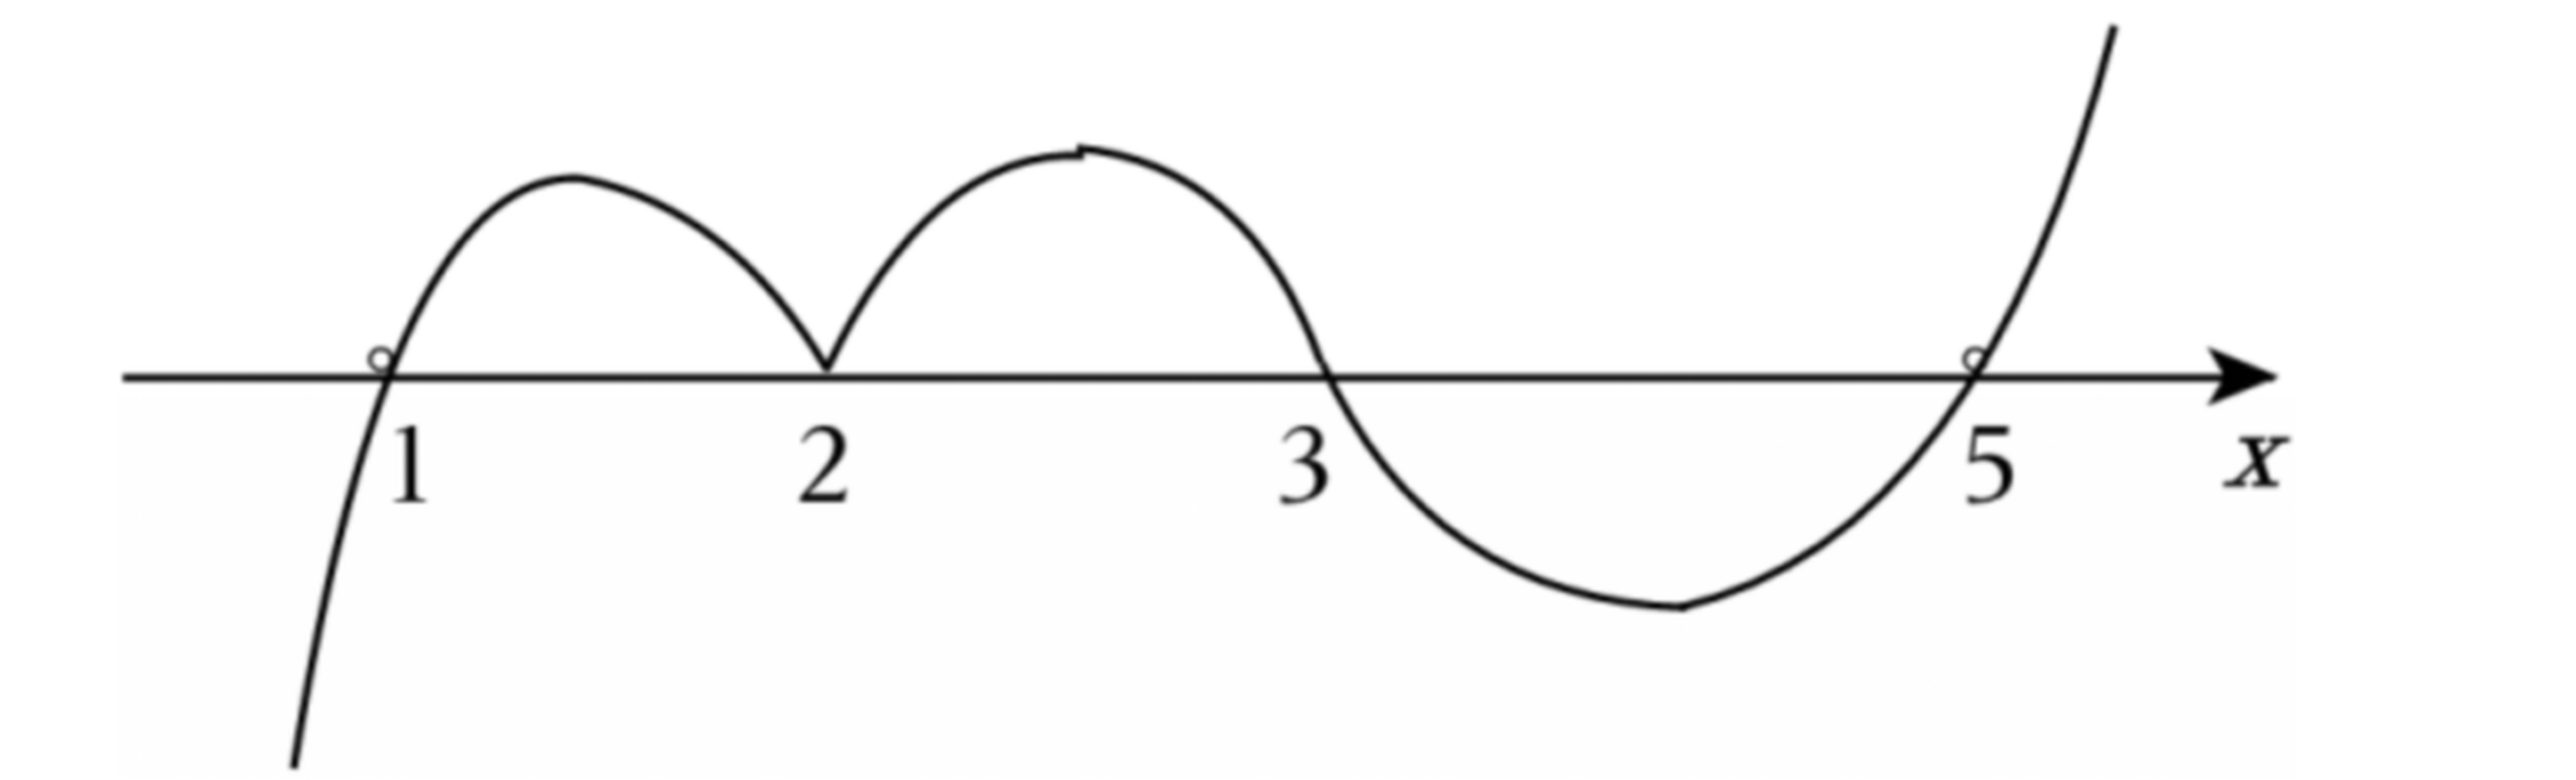
\includegraphics[width=0.62\textwidth]{figures/gao145_q16_a3.png}
\end{center}
\step{得不等式的解集为 $\{x\mid x<1\text{ 或 }x=2\text{ 或 }3\leqslant x<5\}$，}
\step{对应的正整数解为 $2$，$3$，$4$，满足题意，故排除 $B$、$D$；}
\step{当 $a=7$ 时，}
\begin{center}
% a=7 数轴标根图取 06 页，去粉色水印、去色、4× LANCZOS 放大；仅答案版出
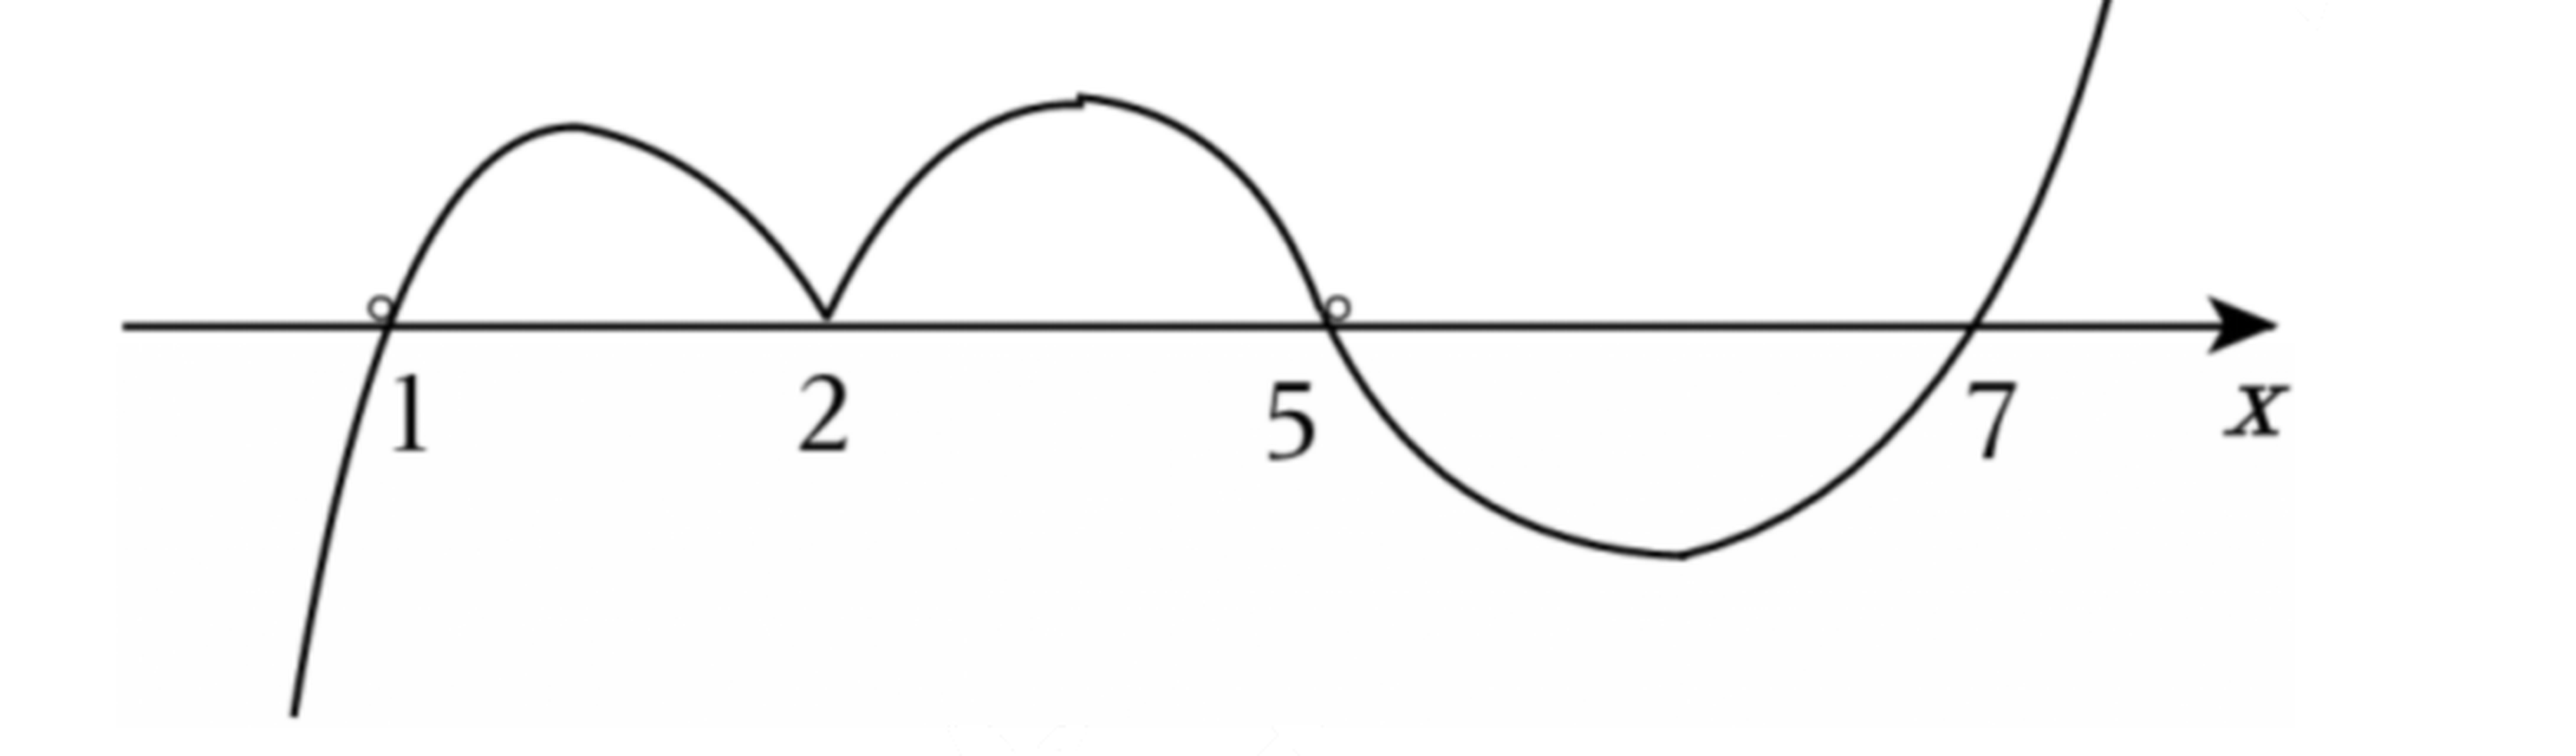
\includegraphics[width=0.62\textwidth]{figures/gao145_q16_a7.png}
\end{center}
\step{得不等式的解集为 $\{x\mid x<1\text{ 或 }x=2\text{ 或 }5<x\leqslant7\}$，}
\step{对应的正整数解为 $2$，$6$，$7$，满足题意，故 $A$ 正确，$C$ 错误.}
\step{故选 $A$.}
\solend
\fi

\end{enumerate}

\bigsec{三、解答题}

\begin{enumerate}
\setcounter{enumi}{16}

% 第 17 题：题干在 06 页、解析续至 07 页，按印刷行断，共 7 行；
% "lg(10÷5)" 的除号照录 \div
\item (1) 已知 $a+a^{-1}=6$，求 $a^2+a^{-2}$ 及 $a^{\frac12}-a^{-\frac12}$ 的值；

(2) 已知 $\lg5=a$，$\lg6=b$，用 $a$、$b$ 分别表示 $\lg2$、$\lg3$、$\lg300$ 和 $\log_{12}15$.

\ifanswer
\solbegin
\step{(1) 因为 $a+a^{-1}=6$，}
\step{所以 $a^2+a^{-2}=(a+a^{-1})^2-2\cdot a\cdot a^{-1}=6^2-2=34$，}
\step{因为 $\left(a^{\frac12}-a^{-\frac12}\right)^2=a-2+a^{-1}=6-2=4$，所以 $a^{\frac12}-a^{-\frac12}=\pm2$；}
\step{(2) $\lg2=\lg(10\div5)=\lg10-\lg5=1-a$，}
\step{$\lg3=\lg(6\div2)=\lg6-\lg2=b-(1-a)=a+b-1$，}
\step{$\lg300=\lg(3\times10^2)=\lg3+\lg10^2=a+b-1+2=a+b+1$，}
\step{所以 $\log_{12}15=\dfrac{\lg15}{\lg12}=\dfrac{\lg3+\lg5}{\lg3+\lg2^2}=\dfrac{a+b-1+a}{a+b-1+2(1-a)}=\dfrac{2a+b-1}{b-a+1}$.}
\solend
\fi

% 第 18 题：题干在 07 页、解析续至 08 页（2 问、分类讨论很长），按印刷行断共 25 行；
% 本卷 Q18 用"图像"（Q13/Q14 用"图象"），逐处照录不统一
\item 已知 $f(x)=(m^2-3m+1)x^{m^2-4m-1}$，$y=f(x)$ 为幂函数且在 $(0,+\infty)$ 上是严格减函数.

(1) 求实数 $m$ 的值以及相应的函数表达式；

(2) 若 $y=f(x)$ 的图像关于 $y$ 轴对称，解关于 $x$ 的不等式 $(x+2)^{1-m}<(3x-1)^{1-m}$.

\ifanswer
\solbegin
\step{(1) 由幂函数的定义得 $m^2-3m+1=1$，}
\step{整理得 $m^2-3m=0$，解得 $m=0$ 或 $m=3$，}
\step{由于 $y=f(x)$ 在 $(0,+\infty)$ 上为严格减函数，}
\step{因此幂函数的指数需满足 $m^2-4m-1<0$，}
\step{当 $m=3$ 时，指数为 $3^2-4\times3-1=-4<0$，满足严格递减条件，}
\step{此时函数表达式为 $f(x)=x^{-4}$，}
\step{当 $m=0$ 时，指数为 $0^2-4\times0-1=-1<0$，满足严格递减条件，}
\step{此时函数表达式为 $f(x)=x^{-1}$，}
\step{所以满足条件的实数 $m$ 为 $0$ 或 $3$，}
\step{对应的函数表达式分别为 $f(x)=x^{-1}$、$f(x)=x^{-4}$；}
\step{(2) 函数图像关于 $y$ 轴对称即函数为偶函数，}
\step{对于 $f(x)=x^{-1}=\dfrac1x$，定义域为 $(-\infty,0)\cup(0,+\infty)$，}
\step{满足 $f(-x)=-f(x)$，为奇函数，图像关于原点对称，}
\step{不满足关于 $y$ 轴对称的条件；}
\step{对于 $f(x)=x^{-4}=\dfrac{1}{x^4}$，定义域为 $(-\infty,0)\cup(0,+\infty)$，}
\step{满足 $f(-x)=f(x)$，为偶函数，图像关于 $y$ 轴对称，}
\step{因此符合条件的 $m$ 值为 $3$，}
\step{将 $m=3$ 代入关于 $x$ 的不等式 $(x+2)^{1-m}<(3x-1)^{1-m}$，}
\step{得 $(x+2)^{1-3}<(3x-1)^{1-3}$，即 $(x+2)^{-2}<(3x-1)^{-2}$，}
\step{因为负指数幂的底数不能为 $0$，所以 $x+2\ne0$ 且 $3x-1\ne0$，}
\step{即 $x\ne-2$ 且 $x\ne\dfrac13$，}
\step{不等式可变形为 $\dfrac{1}{(x+2)^2}<\dfrac{1}{(3x-1)^2}$，}
\step{整理得 $(3x-1)^2<(x+2)^2$，即 $8x^2-10x-3<0$，}
\step{解得 $-\dfrac14<x<\dfrac32$，又 $x\ne-2$ 且 $x\ne\dfrac13$，}
\step{所以不等式的解集为 $\left(-\dfrac14,\dfrac13\right)\cup\left(\dfrac13,\dfrac32\right)$.}
\solend
\fi

% 第 19 题：题干在 08 页、解析续至 09 页，按印刷行断，共 14 行；
% 判别式 cases 块内"△=4a²−16a<0"原卷印扁等边三角 \triangle
%（放大 09 页 zz09_delta.png 与 Q12 高 \Delta 并排确认），逐处照录不统一
\item 已知 $f(x)=ax^2+2ax+4$，$a\in\R$.

(1) 若关于 $x$ 的不等式 $f(x)>0$ 在实数集 $\R$ 上恒成立，求实数 $a$ 的取值范围；

(2) 当 $a<0$ 时，解关于 $x$ 的不等式 $f(x)>(a+1)x+5$.

\ifanswer
\solbegin
\step{(1) 由题意得，关于 $x$ 的不等式 $f(x)>0$ 在实数集 $\R$ 上恒成立，}
\step{即 $ax^2+2ax+4>0$ 在实数集 $\R$ 上恒成立，}
\step{当 $a=0$ 时，不等式为 $4>0$ 恒成立，符合题意；}
\step{当 $a\ne0$ 时，则 $\begin{cases}a>0\\\triangle=4a^2-16a<0\end{cases}$，解得 $0<a<4$.}% 判别式原卷印扁等边三角 $\triangle$，照录
\step{综上所述，实数 $a$ 的取值范围为 $[0,4)$.}
\step{(2) $f(x)=ax^2+2ax+4$，}
\step{当 $a<0$ 时，不等式 $f(x)>(a+1)x+5$ 即为 $ax^2+(a-1)x-1>0$，}
\step{即 $(ax-1)(x+1)>0$，即 $\left(x-\dfrac1a\right)(x+1)<0$，}
\step{当 $a<-1$，即 $\dfrac1a>-1$ 时，解得 $-1<x<\dfrac1a$；}
\step{当 $a=-1$，即 $\dfrac1a=-1$ 时，解得 $x\in\varnothing$；}
\step{当 $-1<a<0$，即 $\dfrac1a<-1$ 时，解得 $\dfrac1a<x<-1$.}
\step{综上所述，当 $a<-1$ 时，不等式的解集为 $\left\{x\mid -1<x<\dfrac1a\right\}$；}
\step{当 $a=-1$ 时，不等式的解集为 $\varnothing$；}
\step{当 $-1<a<0$ 时，不等式的解集为 $\left\{x\mid \dfrac1a<x<-1\right\}$.}
\solend
\fi

% 第 20 题：菜园靠墙图为题目配图（三版都出），题干写"如图"；
% 题干在 09 页（含图）、解析续至 10 页，按印刷行断，共 13 行
\needvspace{8cm}
\item 如图，某人计划用篱笆围成一个一边靠墙（墙足够长）的矩形菜园. 设菜园的长为 $x$ 米，宽为 $y$ 米.

\begin{center}
% 矩形菜园靠墙图取 09 页右下，去粉色水印、去色、4× LANCZOS 放大
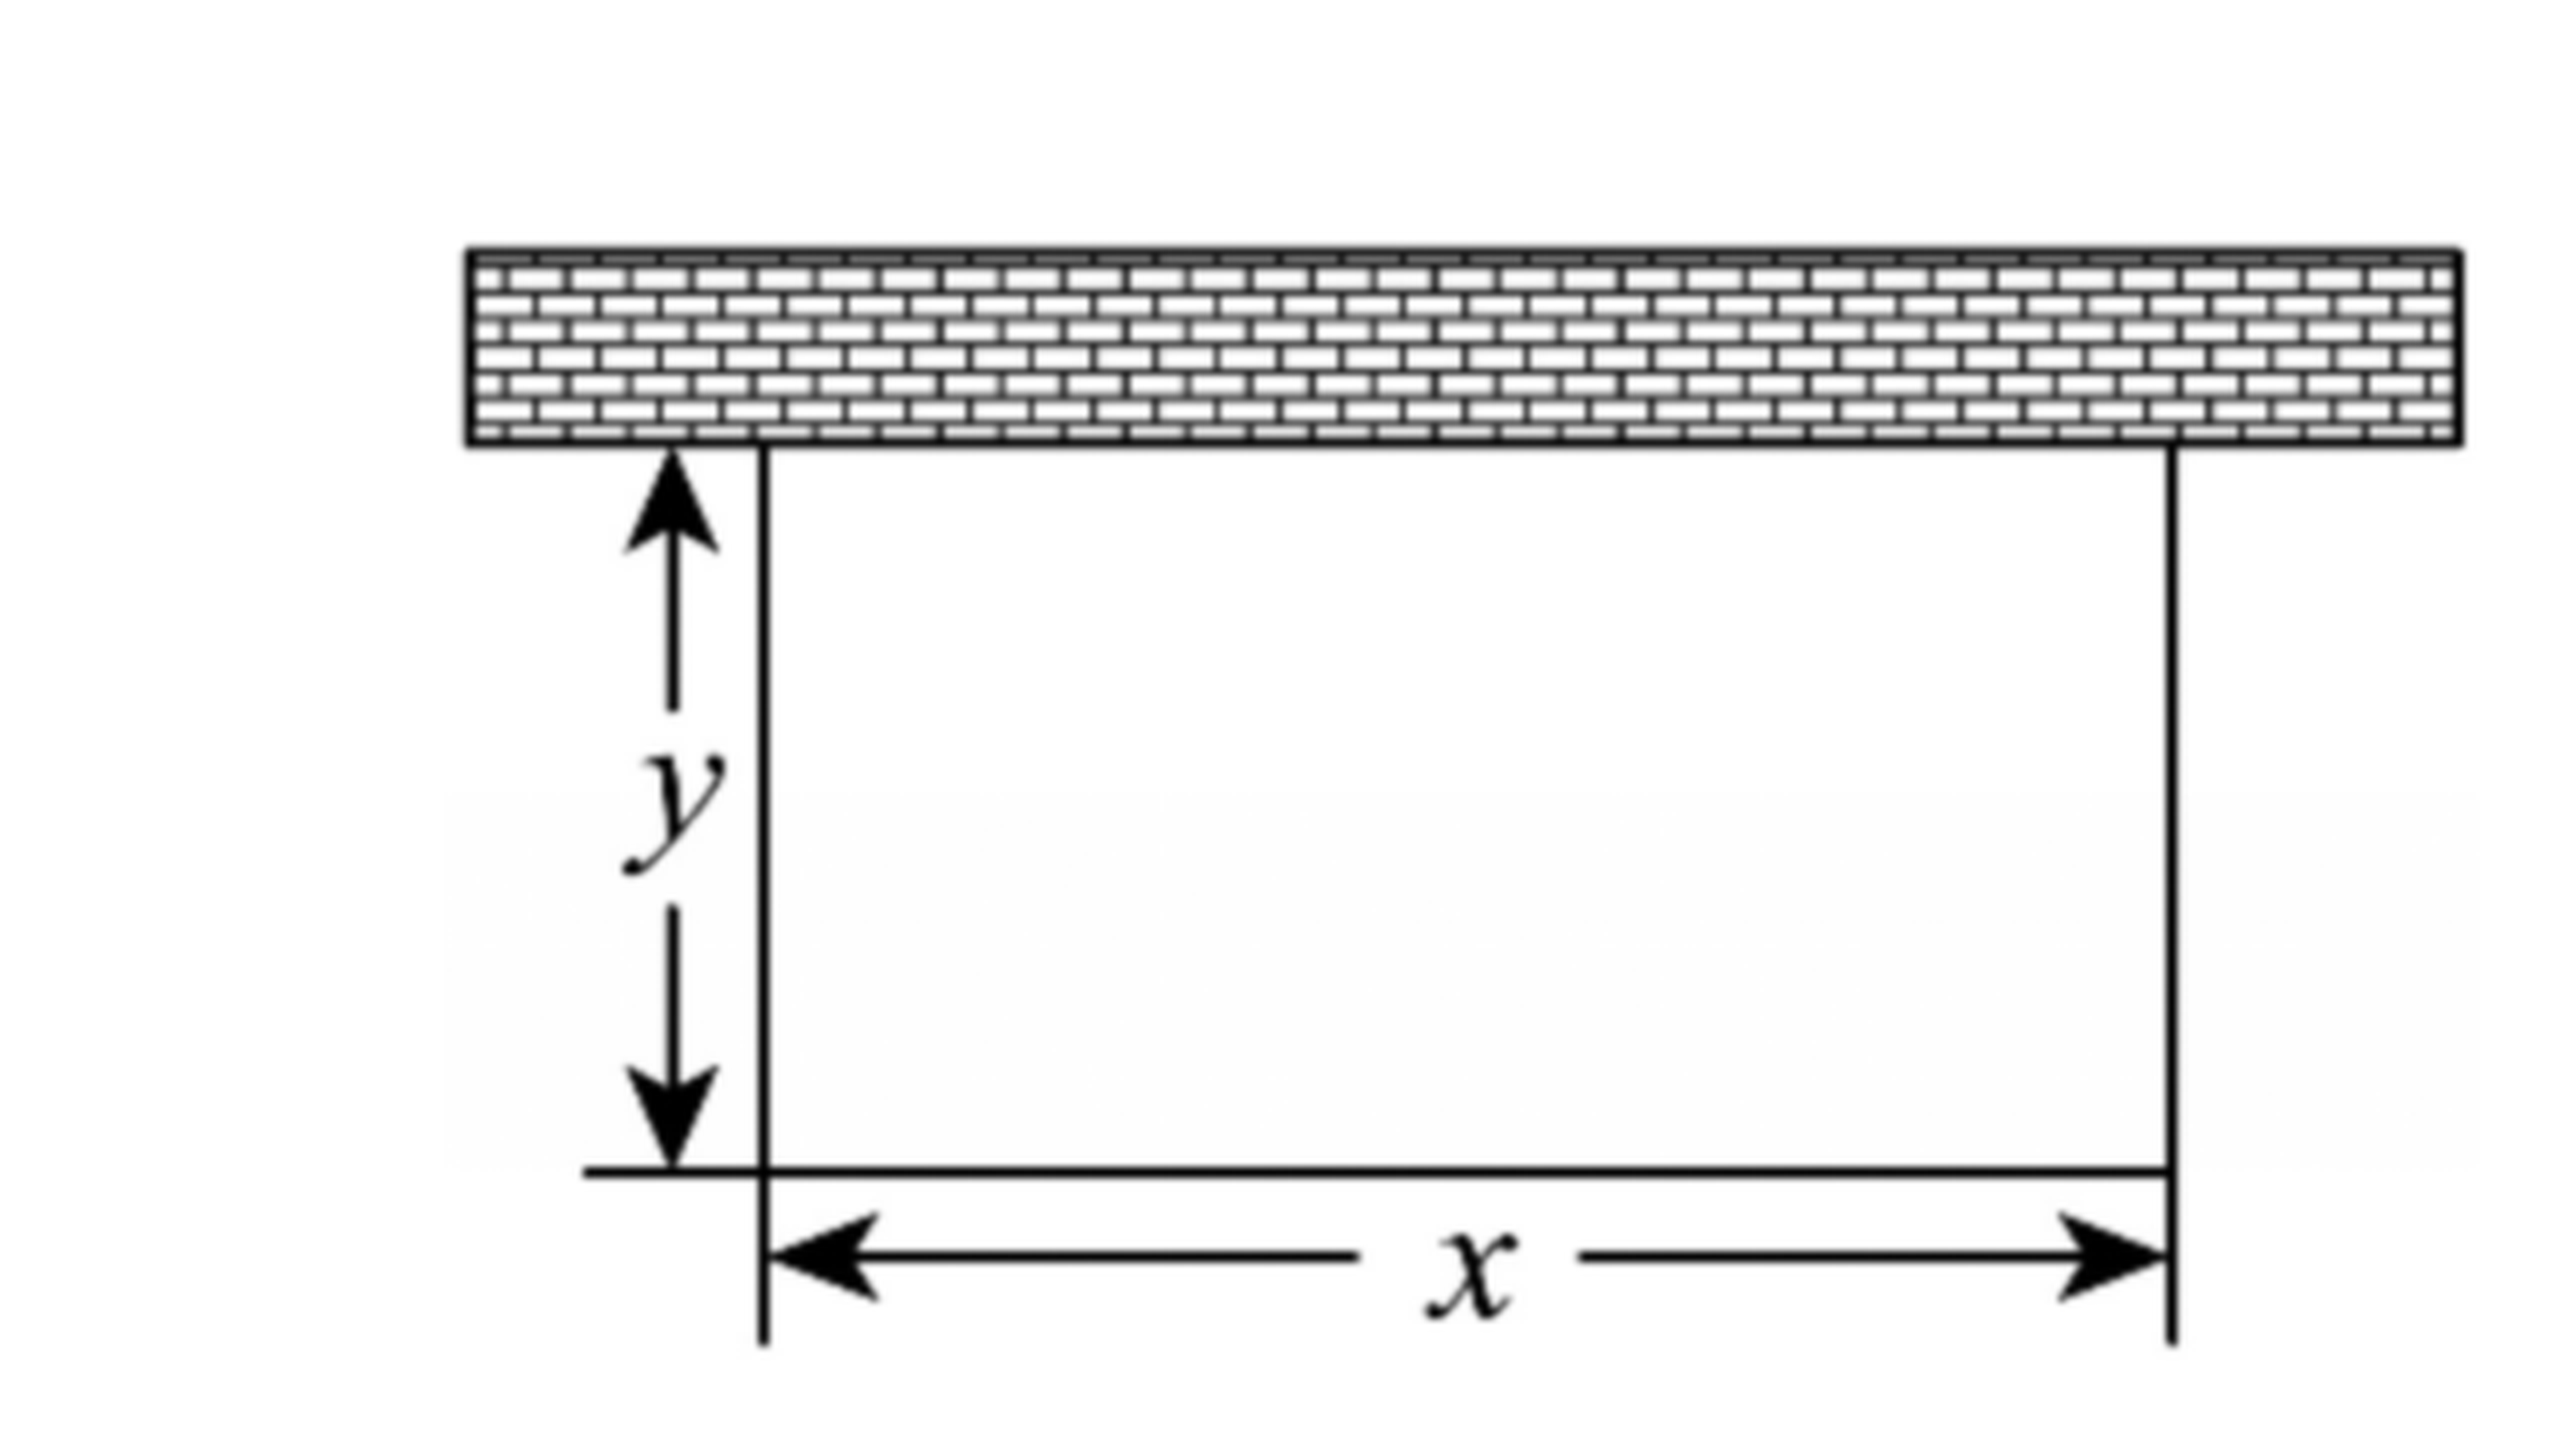
\includegraphics[width=0.55\textwidth]{figures/gao145_q20.png}
\end{center}

(1) 若菜园面积为 72 平方米，则 $x$、$y$ 为何值时，所用篱笆总长最小？

(2) 若 $x$、$y$ 满足 $x+y-xy+63=0$，则菜园面积最小为多少平方米？

\ifanswer
\solbegin
\step{(1) 由题意得，菜园的面积 $S=xy=72$，且 $x>0$，$y>0$，}
\step{所用篱笆总长 $L=x+2y$，}
\step{由基本不等式得 $x+2y\geqslant2\sqrt{x\cdot2y}=2\sqrt{2xy}=2\sqrt{2\times72}=24$，}
\step{当且仅当 $x=2y$ 时取等号，}
\step{联立 $\begin{cases}xy=72\\x=2y\end{cases}$，解得 $\begin{cases}x=12\\y=6\end{cases}$，}
\step{所以当 $x=12$，$y=6$ 时，所用篱笆总长最小；}
\step{(2) 由题意得 $x>0$，$y>0$，且满足 $x+y-xy+63=0$，即 $x+y=xy-63$，}
\step{由基本不等式得 $x+y\geqslant2\sqrt{xy}$，当且仅当 $x=y$ 时取等号，}
\step{所以 $xy-63\geqslant2\sqrt{xy}$. 令 $t=\sqrt{xy}(t>0)$，则 $xy=t^2$，}
\step{上述不等式可化为 $t^2-2t-63\geqslant0$，即 $(t-9)(t+7)\geqslant0$，}
\step{因为 $t>0$，所以 $t+7>0$，故 $t-9\geqslant0$，解得 $t\geqslant9$，所以 $\sqrt{xy}\geqslant9$，}
\step{即 $xy\geqslant81$，当且仅当 $x=y=9$ 时取等号，此时满足 $9+9-81+63=0$，}
\step{所以菜园面积最小为 81 平方米.}
\solend
\fi

% 第 21 题：题干在 10 页、解析续至 11 页（3 问、分类讨论很长），按印刷行断共 22 行；
% 末行"故第 2026 个元素是 2700 之后第一个属于 A 的数，即 2701." 为全卷收尾，
% 无 Q22/Q23、无附加题节；数集 Z/N* 按全稿惯例改 \Z/\N^*
\item 已知集合 $A=\{x\mid x=m^2-n^2$，$m$、$n\in\Z\}$.

(1) 求证：任何奇数 $2k+1(k\in\Z)$ 都是集合 $A$ 中的元素；

(2) 判断偶数 $4k-2(k\in\Z)$ 是否为集合 $A$ 的元素？请说明理由；

(3) 若将集合 $A$ 中的正整数由小到大排列，求出集合 $A$ 中第 2026 个正整数.

\ifanswer
\solbegin
\step{(1) 因为 $x=(k+1)^2-k^2=2k+1(k\in\Z)$，}
\step{所以任何奇数 $2k+1(k\in\Z)$ 都属于集合 $A$；}
\step{(2) 偶数 $4k-2(k\in\Z)$ 不是集合 $A$ 的元素，理由如下：}
\step{由题意得 $x=m^2-n^2=(m-n)(m+n)$，}
\step{当 $m$、$n$ 均为奇数时，设 $m=2k_1+1$，$n=2k_2+1(k_1$、$k_2\in\Z)$，}
\step{则 $m^2-n^2=(2k_1+1)^2-(2k_2+1)^2=(2k_1-2k_2)(2k_1+2k_2+2)$}
\step{$=4(k_1-k_2)(k_1+k_2+1)$，}
\step{因为 $k_1$、$k_2\in\Z$，所以 $k_1-k_2\in\Z$，$k_1+k_2+1\in\Z$，}
\step{从而 $m^2-n^2$ 为 $4$ 的倍数；}
\step{当 $m$、$n$ 均为偶数时，设 $m=2k_1$，$n=2k_2(k_1$、$k_2\in\Z)$，}
\step{$m^2-n^2=4k_1^2-4k_2^2=4(k_1^2-k_2^2)$ 为 $4$ 的倍数；}
\step{当 $m$、$n$ 为一个偶数一个奇数时，不妨设 $m$ 为偶数，$n$ 为奇数，}
\step{设 $m=2k_1$，$n=2k_2+1(k_1$、$k_2\in\Z)$，}
\step{则 $m^2-n^2=4k_1^2-(2k_2+1)^2=4(k_1^2-k_2^2-k_2)-1$ 为奇数.}
\step{无论哪种情况均不满足 $4k-2(k\in\Z)$，}
\step{故偶数 $4k-2(k\in\Z)$ 不是集合 $A$ 的元素；}
\step{(3) 由前两问得，$4$ 的倍数和奇数属于集合 $A$ 中的元素，}
\step{令集合 $A$ 中的正整数元素为 $4k-3$、$4k-1$、$4k(k\in\N^*)$，}
\step{对任意的 $k\in\N^*$，连续的 $4$ 个整数 $4k-3$、$4k-2$、$4k-1$、$4k$ 中}
\step{有三个数 $4k-3$、$4k-1$、$4k$ 都在集合 $A$ 中，}
\step{因为 $2026=3\times675+1$，所以集合 $A$ 中第 $2025$ 个元素为 $4\times675=2700$，}
\step{故第 2026 个元素是 2700 之后第一个属于 $A$ 的数，即 2701.}
\solend
\fi

\end{enumerate}

\end{document}
"
% 紧凑版：xelatex "\def\iscompact{1}% 高一145_市二中学_期中.tex
%   —— 高一上数学"2026-2027 年市二中学高一上期中"（试卷版/答案版/紧凑版）
% 试卷版：xelatex 高一145_市二中学_期中.tex
% 答案版：xelatex "\def\isanswer{1}% 高一145_市二中学_期中.tex
%   —— 高一上数学"2026-2027 年市二中学高一上期中"（试卷版/答案版/紧凑版）
% 试卷版：xelatex 高一145_市二中学_期中.tex
% 答案版：xelatex "\def\isanswer{1}\input{高一145_市二中学_期中.tex}"
% 紧凑版：xelatex "\def\iscompact{1}\input{高一145_市二中学_期中.tex}"
%
% ① 原始材料：微信公众号"魔都数学加油站"文章，连载"27学年高一145"，原文标题
% "27学年高一145——2026-2027年上海市市二中学高一上期中"；
% 原文链接：https://mp.weixin.qq.com/s/6V-i9KE0GWodC-wmd5z8nQ 。
% 正文为 11 张 PNG 页（01/02/03/08/10/11 为 4762×6735，04/05/06/07/09 为 2560×3620，
% 同一篇各页分辨率不同，逐页按各自分辨率裁图核对，别按预览比例换算裁框）。
% 题目下印【答案】或【解析】，为混合体例讲评版：Q3 只印【答案】、无【解析】，其余
% 18 题印【解析】。题目、解析均据原图转录；卷面粉红色水印"魔都数学加油站"及
% 公众号页脚未录入。
% 全卷插图情况（逐页通读 11 页确认，题干写"如图"处均配有图）：
%   · Q14 韦恩图（05 页右侧，全集 U 矩形＋两圆 M/N＋白色交集、灰色阴影＋U/M/N 标注）：
%     题目配图（选择题选项旁），三版都出，裁自 05 页去水印去色 4× 放大存
%     figures/gao145_q14.png；
%   · Q16 两幅数轴标根波浪曲线（06 页，a=3 与 a=7 各一幅，标根法画
%     (x-1)(x-2)^2(x-5)(x-a)≤0 的符号曲线）：【解析】内的配图，仅答案版出，
%     裁 figures/gao145_q16_a3.png / figures/gao145_q16_a7.png（或合并一张），
%     放在答案版条件块内 \solbegin 的 \step 之间（照 高一73 第 16 题成例）；
%   · Q20 矩形菜园靠墙图（09 页右下，灰色砖墙＋矩形菜园＋x/y 标注＋箭头）：
%     题目配图，三版都出，裁自 09 页去水印去色 4× 放大存 figures/gao145_q20.png；
%   其余各页逐页确认无其它题目配图、无表格、亦无"题干写如图而源码漏图"一处。
%
% 卷首标题：原卷印作"2026-2027 年市二中学高一上期中"，年份区间按全稿惯例排 en dash；
% 原卷卷面未印副标题，本稿按同期中卷（高一140／141／143／144）知识模块口径补出
% "集合与常用逻辑用语、不等式、函数"。
%
% 题号体例：本卷共 19 题——一、填空题 3—12（10 题）、二、选择题 13—16（4 题）、
% 三、解答题 17—21（5 题）。三节分别 \setcounter{enumi}{2}／{12}／{16}。
% 原卷从第 3 题起、无第 1、2 题，本稿保留原题号；全卷无附加题节。
%
% ② 与原卷的排版差异：
%   ① 原文从第 3 题起，本稿保留原题号；共 19 题三节；
%   ② 混合体例：原卷 Q3 只印【答案】、无【解析】（"第一步应假设___。
%      【答案】x≤2 或 y≤2"），按 高一140 第 5 题成例提 \ans{}、不补造解析；
%      其余 18 题印【解析】，用 \solbegin…\solend，选择题答案在解析末句"故选 X"
%      （Q13 选 B、Q14 选 D、Q15 选 D、Q16 选 A，逐个放大原图核实）、
%      题干括号 \mbox{（\quad）} 留空、不另提 \ans{}；填空／解答答案落在解析里；
%      答案版【答案】/【解析】标记数 = 19（1 个 \ans ＋ 18 个 \solbegin）= 全卷题数；
%   ③ 原卷卷面未印副标题，本稿按知识模块口径补出；
%   ④ 原卷填空横线按全稿惯例排 \blankline[4.4em]；选择题括号排 \mbox{（\quad）}、
%      选项段前按惯例加 \keepwithprev；解答题不留作答区、不加 \anspace
%      （原卷为讲评版，与 129／131／132／133／136／140／141／143／144 同）；
%   ⑤ 数集：Q9"a、b∈R"、Q12"a∈R"、Q21"m、n∈Z""k∈Z""k∈N*"等原卷印
%      斜体或黑板粗体 R/Z/N，按全稿惯例统一改 \R／\Z／\N^*；绝对值排 \lvert…\rvert，
%      集合描述竖线排 \mid；不等号按全稿惯例排 \leqslant／\geqslant；
%      补集照原卷上划线排 \overline{M}／\overline{N}（Q14 选项 B/C/D 逐处核）；
%      空集记号 \varnothing；\subset（单线⊂）与 \subseteq（带下划线⊆）逐处照录不统一；
%   ⑥ 子题标号 (1)(2)(3) 原卷印半角括号照录；圈数字进数学式用 \text{①}（否则 FONTCHK 挂）；
%      \left…\right 不得拆到不同 $…$ 组；cases 块整体算一个印刷行；
%   ⑦ 题干／解析中的中文弯引号按原卷照录（Q3"若 x+y>4，则 x>2 且 y>2"、
%      Q11"a₁/a₂=b₁/b₂""M=N"、选填"充分非必要""必要非充分""充要""既非充分也非必要"
%      等，含引号内空格），注释内一律 ASCII 引号；数学式内 CJK 用 \text{}；
%   ⑧ 半角逗号在数学组之间是全稿惯例、非笔误（如 Q5"x₁+x₂=6，x₁x₂=√3"、
%      Q7"a>1，b>1"、指数／对数式内逗号），逐处照录别改全角；行末西文句点照录为
%      ASCII `.`；行中全角逗号／顿号照录；
%   ⑨ "图像／图象"逐处照录不统一（Q18"图像关于 y 轴对称"等，核全卷）；
%   ⑩ 判别式 Δ/△ 混用是照录项：Q12 解析"Δ=a²−4a²(2a−3)>0"、
%      Q19 解析"Δ=4a²−16a<0"等，放大原图判断是高 \Delta（等腰偏高、高>宽）
%      还是扁 \triangle，逐处照录不得统一（参照 高一142／144 头注④口径）；
%   ⑪ 一条 \step = 原卷解析的一个印刷行，cases 块整体算一个印刷行；别把原卷折行
%      并起来、别把一行拆多条。Q6 分段讨论、Q12 三个 cases 条件组、Q16 数轴标根、
%      Q18／Q19 分类讨论、Q21 三问均按印刷行逐条断，不丢行；
%   ⑫ Q14 韦恩图为"题干＋选项＋图"整块，加 \needvspace 守卫推走（守卫放 \item 之前，
%      见 高一140 Q14、高一144 Q17 成例与切页审计 B 类坑）；Q20 菜园图同理；
%      三版切页审计均"合计异常：无"；
%   ⑬ 跨页续印按题合并：Q3/4/5/6 在 01 页（Q6 解析续 02 页顶）；Q7/8/9/10 在 02 页
%      （Q10 解析续 03 页）；Q11/12 在 03 页（Q12 解析续 04 页，很长）；
%      Q13 在 04 页末、解析在 05 页顶；Q14/15/16 在 05 页（Q16 解析续 06 页含两幅数轴图）；
%      Q17 在 06 页、解析续 07 页；Q18 在 07 页、解析续 08 页；Q19 在 08 页、解析续 09 页；
%      Q20 在 09 页（含菜园图）、解析续 10 页；Q21 在 10 页、解析续 11 页
%      （末页收尾"故第 2026 个元素是 2700 之后第一个属于 A 的数，即 2701."、
%      无 Q22/Q23、无附加题节）。本稿按题连排，不丢行、不并折行；
%   ⑭ 原卷解析内若有红色"法一／法二"之类小标题，按全稿惯例排 \stepm{标签}{…}
%      （黑体着色、不引入红色、不改 common.sty），头注注明；水印"魔都数学加油站"
%      红色不录入。
%
% ③ 行数复核：一条 \step／\stepm = 原卷解析的一个印刷行，cases 块作一个印刷行计。
%   逐题数（主会话逐页核对定稿）：Q3：0（只印【答案】、提 \ans{}，不计入 \step 账）；
%   Q4：3；Q5：2；Q6：10；Q7：3；Q8：3；Q9：2；Q10：7；Q11：4；Q12：12；
%   Q13：2；Q14：2；Q15：4；Q16：9；Q17：7；Q18：25；Q19：14；Q20：13；Q21：22。
%   合计 144 条 \step（本卷无 \stepm：解析内无红色"法一／法二"类小标题），
%   与原卷逐题印刷行相等。全卷 18 题设 \solbegin…\solend ＋ Q3 一处 \ans{}，
%   答案版【答案】/【解析】标记数 = 19 = 全卷题数。
%
% ④ 判别式／子集符号结论（逐处放大原图照录、不得统一，主会话像素级复核）：
%   判别式全卷 2 处、两形混用逐处照录不统一（参照 高一142／144 头注④口径）：
%     · Q12 解析 cases 块"Δ=a²−4a²(2a−3)>0" 原卷印等腰偏高粗三角（高>宽），
%       照录 \Delta（放大 04 页 /tmp/gao145s2/main_q12_delta.png 确认）；
%     · Q19 解析 cases 块"△=4a²−16a<0" 原卷印扁等边空心三角（宽≈高、细线），
%       照录 \triangle（放大 09 页 /tmp/gao145s2/main_q19_delta.png 确认）。
%   子集／补集：Q14 选项 A `M\cup N`、B `M\cap\overline{N}`（上划线只在 N 上）、
%   C `\overline{M\cup N}`（罩整个 M∪N）、D `\overline{M\cap N}`（罩整个 M∩N，
%   非 \overline{M}\cap N；放大 05 页 /tmp/gao145s2/main_q14_opts.png 确认），
%   阴影为灰色区域＝全集减白色交集，答案 D，照录 \overline{M\cap N}；
%   全集卷无 \subset／\subseteq 混用（本卷集合题用 \cup／\cap／\overline{}）；
%   空集 \varnothing（Q19 解析 x∈\varnothing）；数集 \R／\Z／\N^* 归一见 ② ⑤。
%
% ⑤ 存疑照录（放大原图确认，照录未改、正文对应处另有 % 注）：
%   1. Q3 题干"若 x+y>4，则 x>2 且 y>2" 后"时"前留一空格、弯引号内空格照录；
%      该卷混合体例（Q3 只印【答案】、提 \ans{}）见 ② ②。
%   2. Q4／Q5 解析中的"1，3，5 和 6"、"x₁+x₂=6,x₁x₂=√3" 等半角／全角逗号
%      逐处照原卷（放大 01 页确认），数学式内半角逗号为全稿惯例、非笔误。
%   3. Q14 选项 D 上划线罩住整个 M∩N（而非仅罩 M），照录 \overline{M\cap N}。
%   4. Q12 判别式高 \Delta 与 Q19 判别式扁 \triangle 两形混用，逐处照录不统一（见 ④）。
%   全卷除此 4 类外未发现其它笔误／自相矛盾处。
%
% ⑥ 跨页续印按题合并说明：见 ② ⑬。
%
\documentclass[a4paper,11pt]{article}
\usepackage{common}

\begin{document}

\examtitlest[3]{2026--2027 年市二中学高一上期中}{集合与常用逻辑用语、不等式、函数}

\bigsec{一、填空题}

\begin{enumerate}
\setcounter{enumi}{2}

% 第 3 题：原卷只印【答案】、无【解析】（放大 01 页确认），按 高一140 第 5 题成例
% 提 \ans{}、不补造解析；题干中文弯引号与"时"前空格照录
\item 用反证法证明命题：“若 $x+y>4$，则 $x>2$ 且 $y>2$” 时，第一步应假设\blankline[4.4em].

\ifanswer
\ans{$x\leqslant2$ 或 $y\leqslant2$}
\fi

% === Q4 ===
\item 设集合 $M$ 满足 $\{1,3,5,6\}\cup M=\{1,2,3,4,5,6\}$，则满足条件的所有 $M$ 的个数为\blankline[4.4em].

\ifanswer
\solbegin
\step{集合 $M$ 满足 $\{1,3,5,6\}\cup M=\{1,2,3,4,5,6\}$，}
\step{则 $M$ 中必含有 $2$ 和 $4$，$1$，$3$，$5$ 和 $6$ 可以选也可不选，}
\step{则满足条件的所有 $M$ 的数目相当于集合 $\{1,3,5,6\}$ 的子集的个数 $2^4=16$.}
\solend
\fi

% === Q5 ===
\item 已知方程 $x^2-6x+\sqrt3=0$ 的两根为 $x_1$ 和 $x_2$，则 $(x_1-x_2)^2=$\blankline[4.4em].

\ifanswer
\solbegin
\step{因为方程 $x^2-6x+\sqrt3=0$ 的两根为 $x_1$ 和 $x_2$，所以 $x_1+x_2=6,x_1x_2=\sqrt3$，}% 数学式内半角逗号为全稿惯例，照录
\step{所以 $(x_1-x_2)^2=(x_1+x_2)^2-4x_1x_2=36-4\sqrt3$.}
\solend
\fi

% 第 6 题：题干在 01 页，解析续至 02 页顶（末 2 行），按印刷行逐条断，共 10 行
\item 不等式 $\lvert x-2026\rvert+\lvert x-2029\rvert>3$ 的解集是\blankline[4.4em].

\ifanswer
\solbegin
\step{当 $x<2026$ 时，$x-2026<0$，$x-2029<0$，}
\step{原不等式可化为 $(2026-x)+(2029-x)>3$，解得 $x<2026$，}
\step{故此时，不等式的解为 $x<2026$；}
\step{当 $2026\leqslant x\leqslant2029$ 时，$x-2026\geqslant0$，$x-2029\leqslant0$，}
\step{原不等式可化为 $(x-2026)+(2029-x)>3$，即 $3>3$，显然不成立，}
\step{故此时，不等式无解；}
\step{当 $x>2029$ 时，$x-2026>0$，$x-2029>0$，}
\step{原不等式可化为 $(x-2026)+(x-2029)>3$，解得 $x>2029$，}
\step{故此时，不等式的解为 $x>2029$.}
\step{综上，原不等式的解集为 $(-\infty,2026)\cup(2029,+\infty)$.}
\solend
\fi

% === Q7 ===
\item 已知 $a>1$，$b>1$，若 $\log_a b+\log_b a=2$，且 $ab=2$，则 $\log_2(a+b)=$\blankline[4.4em].

\ifanswer
\solbegin
\step{由 $\log_a b+\log_b a=2$，$a>1$，$b>1$，得 $\log_a b+\dfrac{1}{\log_a b}=2$，}
\step{即 $(\log_a b)^2-2\log_a b+1=0$，则 $(\log_a b-1)^2=0$，解得 $\log_a b=1$，即 $a=b$，}
\step{又 $ab=2$，所以 $a=b=\sqrt2$，所以 $\log_2(a+b)=\log_2 2\sqrt2=\log_2 2^{\frac32}=\dfrac32$.}
\solend
\fi

% === Q8 ===
\item 已知 $m>0$，$n>0$，且 $m+n=1$，则 $\dfrac1m+\dfrac4n$ 的最小值为\blankline[4.4em].

\ifanswer
\solbegin
\step{由 $m>0$，$n>0$，$m+n=1$，}
\step{则 $\dfrac1m+\dfrac4n=(m+n)\left(\dfrac1m+\dfrac4n\right)=5+\dfrac nm+\dfrac{4m}n\geqslant5+2\sqrt{\dfrac nm\cdot\dfrac{4m}n}=9$，}
\step{当且仅当 $n=2m=\dfrac23$ 时，上式取得等号，故最小值为 $9$.}
\solend
\fi

% === Q9 ===
\item 已知 $a$、$b\in\R$，且 $3a+2b=1$，则 $8^a+4^b$ 最小值为\blankline[4.4em].

\ifanswer
\solbegin
\step{因为 $3a+2b=1$，所以 $8^a+4^b=2^{3a}+2^{2b}\geqslant2\sqrt{2^{3a+2b}}=2\sqrt2$，}
\step{当且仅当 $3a=2b$ 时取等号，故最小值为 $2\sqrt2$.}
\solend
\fi

% 第 10 题：题干在 02 页、解析续至 03 页顶，按印刷行断，共 7 行
\item 已知关于 $x$ 的不等式 $ax^2+bx+c>0$ 的解集为 $\{x\mid 1<x<2\}$，则关于 $x$ 的不等式 $bx^2-ax+c<0$ 的解集为\blankline[4.4em].

\ifanswer
\solbegin
\step{已知关于 $x$ 的不等式 $ax^2+bx+c>0$ 的解集为 $\{x\mid 1<x<2\}$，}
\step{由解集为 $1<x<2$ 且二次函数在两根之间为正，得 $a<0$，两个根为 $1$，$2$，}
\step{所以 $ax^2+bx+c=a(x-1)(x-2)=ax^2-3ax+2a$，}
\step{比较系数得 $b=-3a$，$c=2a$.}
\step{于是 $bx^2-ax+c=-3ax^2-ax+2a=-a(3x-2)(x+1)$，}
\step{$a<0$，故 $bx^2-ax+c<0$ 等价于 $(3x-2)(x+1)<0$，解得 $-1<x<\dfrac23$，}
\step{故 $bx^2-ax+c<0$ 的解集为 $\left\{x\mid -1<x<\dfrac23\right\}$.}
\solend
\fi

% 第 11 题：题干引号内空格照录（放大 03 页确认），四组选填引号亦同；
% 结论"故为必要非充分条件"照录，解析共 4 个印刷行
\item 设 $a_1$、$b_1$、$a_2$、$b_2$ 均为非零实数，不等式 $a_1x+b_1>0$ 和 $a_2x+b_2>0$ 的解集分别为集合 $M$、$N$，那么 “ $\dfrac{a_1}{a_2}=\dfrac{b_1}{b_2}$ ” 是 “ $M=N$ ” 的\blankline[4.4em]条件（选填 “ 充分非必要 ”、“ 必要非充分 ”、“ 充要 ” 和 “ 既非充分也非必要 ”）.

\ifanswer
\solbegin
\step{当 $a_1=b_1=1$，$a_2=b_2=-1$ 时，满足 $\dfrac{a_1}{a_2}=\dfrac{b_1}{b_2}$，}
\step{但是 $M=N$ 不成立，即充分性不成立；}
\step{若 $M=N$ 时，$\dfrac{a_1}{a_2}=\dfrac{b_1}{b_2}$ 一定成立，即必要性成立.}
\step{故为必要非充分条件.}
\solend
\fi

% 第 12 题：题干在 03 页、解析续至 04 页（很长，含 3 个 cases 条件组），
% 按印刷行逐条断共 12 行；cases 块整体算一个印刷行
\item 已知 $f(x)=\dfrac{ax+3}{x-2}$（常数 $a\in\R$）. 函数 $y=f(x)$ 在区间 $[3,+\infty)$ 上是严格减函数，且函数值不恒为负. 若关于 $x$ 的方程 $f(x)=\dfrac{a}{ax-1}$ 有两个不相等的实数根 $x_1$ 和 $x_2$，则 $a$ 的取值范围是\blankline[4.4em].

\ifanswer
\solbegin
\step{$f(x)=\dfrac{ax+3}{x-2}=a+\dfrac{3+2a}{x-2}$，定义域 $(-\infty,2)\cup(2,+\infty)$，}
\step{由于 $y=f(x)$ 在区间 $[3,+\infty)$ 上是严格减函数，且函数值不恒为负，}
\step{所以 $\begin{cases}3+2a>0\\a+\dfrac{3+2a}{3-2}\geqslant0\end{cases}\Rightarrow a\geqslant-1$，}
\step{若关于 $x$ 的方程 $f(x)=\dfrac{a}{ax-1}$ 有两个不相等的实数根 $x_1$ 和 $x_2$，}
\step{则 $\dfrac{ax+3}{x-2}=\dfrac{a}{ax-1}$，即 $(ax+3)(ax-1)=a(x-2)$，$x\ne2$ 且 $ax-1\ne0$，}
\step{当 $a\ne0$ 且 $a\geqslant-1$ 时，$(ax+3)(ax-1)=a(x-2)$，$x\ne2$ 且 $ax-1\ne0$，}
\step{可化为 $\begin{cases}a^2x^2+ax+2a-3=0\\x\ne2,x\ne\dfrac1a\end{cases}$，}
\step{要使方程有两个不相等的实数根 $x_1$ 和 $x_2$，}
\step{则 $\begin{cases}\Delta=a^2-4a^2(2a-3)>0\\a\geqslant-1\text{且}a\ne0\\4a^2+2a+2a-3\ne0\\a^2\cdot\dfrac1{a^2}+a\cdot\dfrac1a+2a-3\ne0\end{cases}\Rightarrow\begin{cases}a<\dfrac{13}{8}\\a\geqslant-1\text{且}a\ne0\\a\ne\dfrac12\text{且}a\ne-\dfrac32\\a\ne\dfrac12\end{cases}$，}% 判别式原卷印等腰偏高三角 $\Delta$，照录（放大 04 页 zz04_delta.png 确认）
\step{得 $-1\leqslant a<\dfrac{13}{8}$ 且 $a\ne0,a\ne\dfrac12$；}
\step{当 $a=0$ 时，方程无解；}
\step{所以 $a$ 的取值范围是 $[-1,0)\cup\left(0,\dfrac12\right)\cup\left(\dfrac12,\dfrac{13}{8}\right)$.}
\solend
\fi

\end{enumerate}

\bigsec{二、选择题}

\begin{enumerate}
\setcounter{enumi}{12}

% 第 13 题：题干在 04 页末、解析在 05 页顶；"图象"照录（本卷 Q13、Q14 用"图象"）
\item 已知幂函数 $f(x)$ 的图象过点 $\left(7,\dfrac{1}{\sqrt7}\right)$，则 $f(x)=$\mbox{（\quad）}

\keepwithprev
A. $x^{-2}$\qquad B. $x^{-\frac12}$\qquad C. $x^{\frac12}$\qquad D. $x^2$

\ifanswer
\solbegin
\step{设幂函数 $f(x)=x^\alpha(\alpha\in\R)$，因为幂函数的图象过点 $\left(7,\dfrac{1}{\sqrt7}\right)$，}
\step{所以 $7^\alpha=\dfrac{1}{\sqrt7}=7^{-\frac12}$，所以 $\alpha=-\dfrac12$，故 $f(x)=x^{-\frac12}$. 故选 $B$.}
\solend
\fi

% 第 14 题：韦恩图为题目配图（三版都出），"题干＋选项＋图"整块，needvspace
% 守卫放在 \item 之前（Q14 为选择题节内第二题，不会让节标题孤落页末）；
% D 选项上划线罩住整个 M∩N（放大 05 页 zz05_q14D.png 确认，非 \overline{M}\cap N）
\needvspace{9cm}
\item 已知全集 $U$ 和集合 $M$、$N$，用集合语言表示图中的阴影部分，正确的是\mbox{（\quad）}

\keepwithprev
A. $M\cup N$\qquad B. $M\cap\overline{N}$\qquad C. $\overline{M\cup N}$\qquad D. $\overline{M\cap N}$

\begin{center}
% 韦恩图取 05 页右侧，去粉色水印、去色、4× LANCZOS 放大
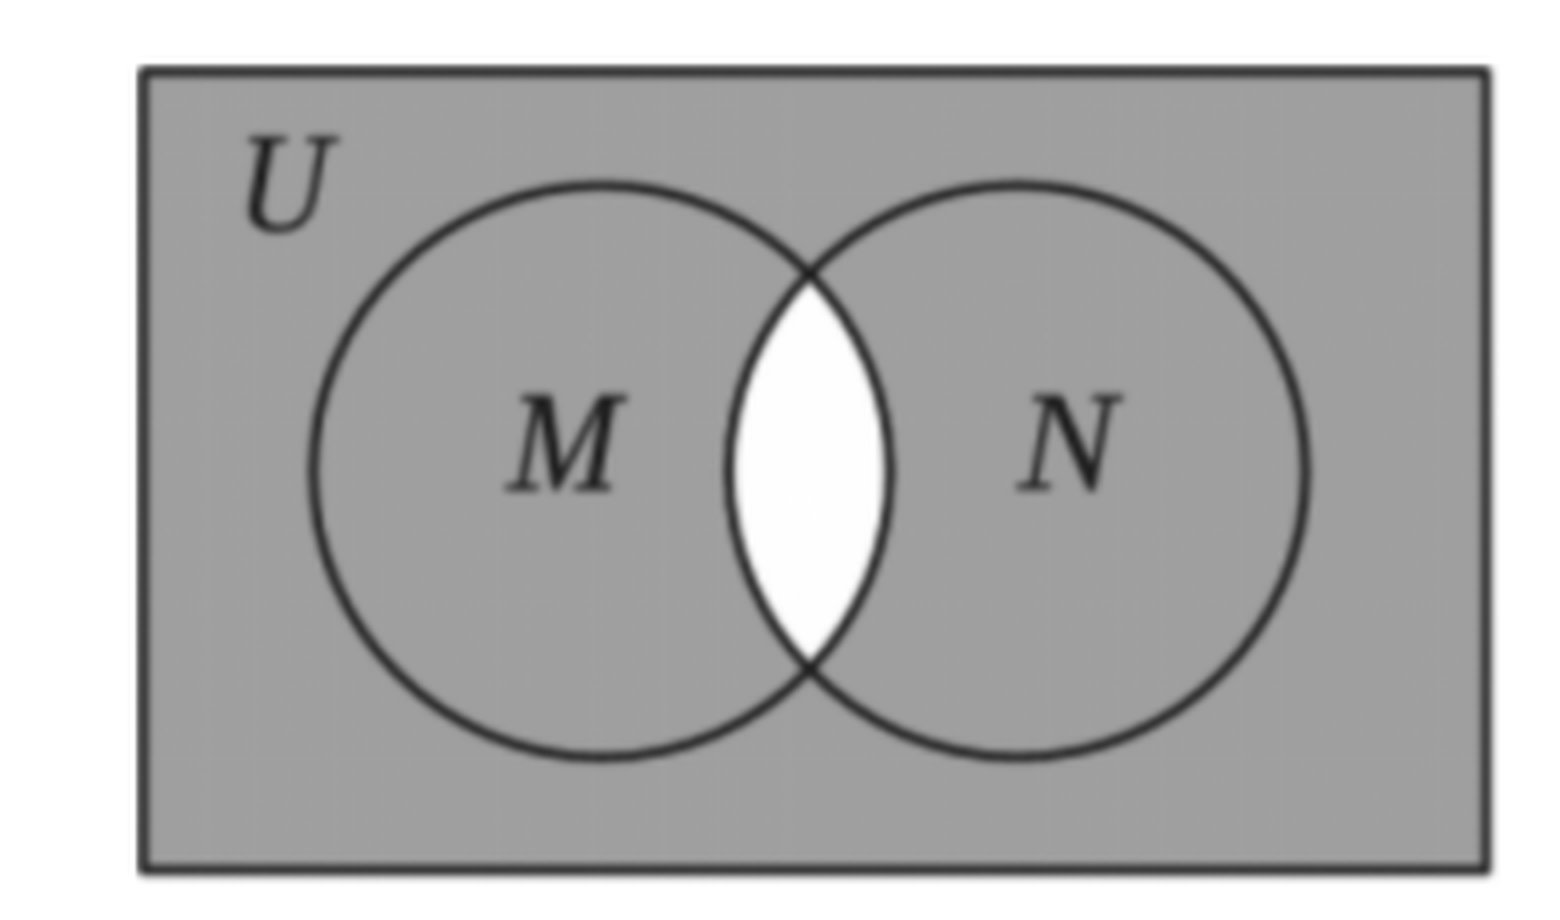
\includegraphics[width=0.40\textwidth]{figures/gao145_q14.png}
\end{center}

\ifanswer
\solbegin
\step{由韦恩图得图中白色区域为集合 $M\cap N$，所以阴影部分表示的集合为 $\overline{M\cap N}$.}
\step{故选 $D$.}
\solend
\fi

% === Q15 ===
\item 已知 $x>-2$，则 $x+\dfrac{1}{x+2}$ 的最小值为\mbox{（\quad）}

\keepwithprev
A. 3\qquad B. 2\qquad C. 1\qquad D. 0

\ifanswer
\solbegin
\step{$x>-2$，则 $x+2>0$，}
\step{所以 $x+\dfrac{1}{x+2}=(x+2)+\dfrac{1}{x+2}-2\geqslant2\sqrt{(x+2)\cdot\dfrac{1}{x+2}}-2=0$，}
\step{当且仅当 $x+2=\dfrac{1}{x+2}$，即 $x=-1$ 时取等号，所以 $x+\dfrac{1}{x+2}$ 的最小值为 $0$.}
\step{故选 $D$.}
\solend
\fi

% 第 16 题：题干在 05 页、解析续至 06 页；两幅数轴标根波浪曲线是【解析】内配图，
% 仅答案版出，放在答案版条件块内 \solbegin 的 \step 之间（照 高一73 第 16 题成例）
\item 关于 $x$ 的不等式 $\dfrac{(x-a)(x-2)^2}{(x-1)(x-5)}\leqslant0$ 的解集中恰有 3 个正整数，则实数 $a$ 的取值范围是\mbox{（\quad）}

\keepwithprev
A. $(-\infty,3]\cup[7,8)$\qquad B. $(-\infty,3)\cup[7,8)$\qquad C. $(-\infty,3]\cup(7,8]$\qquad D. $(-\infty,3)\cup(7,8]$

\ifanswer
\solbegin
\step{由题意，不等式 $\dfrac{(x-a)(x-2)^2}{(x-1)(x-5)}\leqslant0$，}
\step{可化为 $\begin{cases}(x-1)(x-2)^2(x-5)(x-a)\leqslant0\\x\ne1\text{且}x\ne5\end{cases}$，由数轴标根法，}
\step{当 $a=3$ 时，}
\begin{center}
% a=3 数轴标根图取 06 页，去粉色水印、去色、4× LANCZOS 放大；仅答案版出
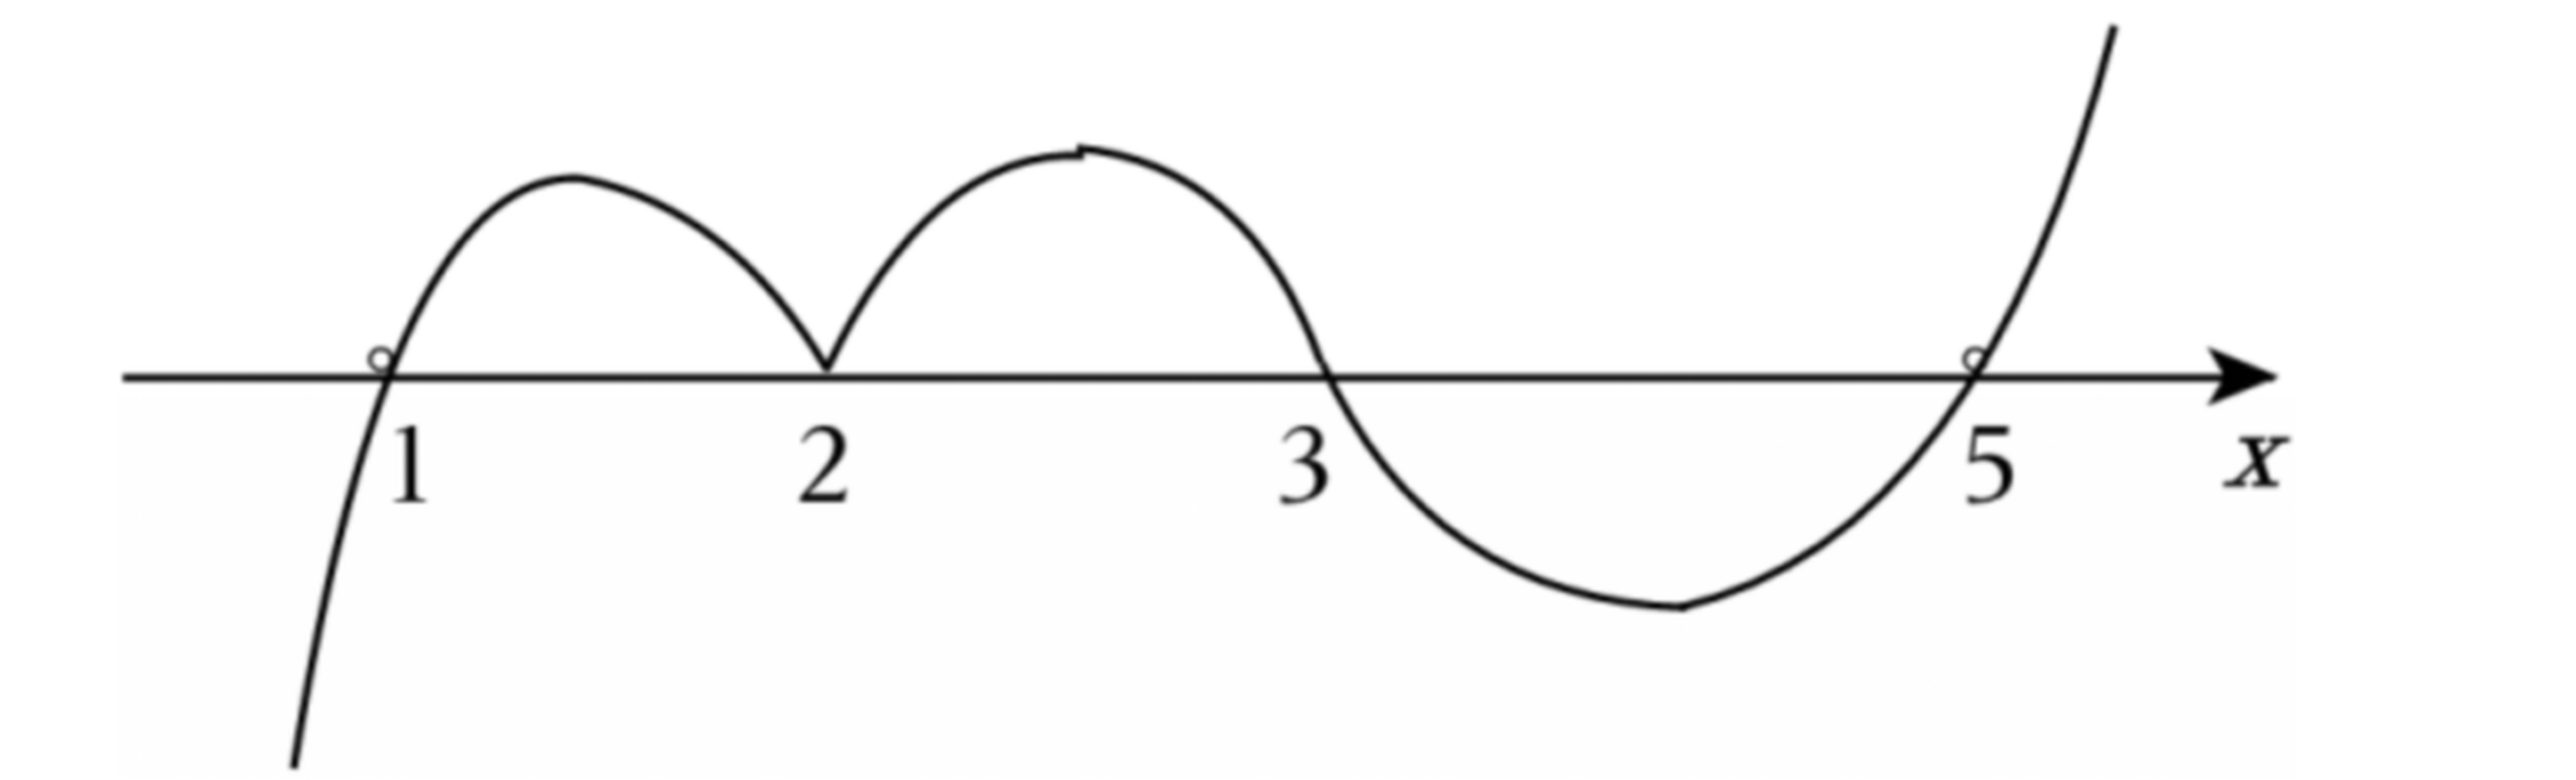
\includegraphics[width=0.62\textwidth]{figures/gao145_q16_a3.png}
\end{center}
\step{得不等式的解集为 $\{x\mid x<1\text{ 或 }x=2\text{ 或 }3\leqslant x<5\}$，}
\step{对应的正整数解为 $2$，$3$，$4$，满足题意，故排除 $B$、$D$；}
\step{当 $a=7$ 时，}
\begin{center}
% a=7 数轴标根图取 06 页，去粉色水印、去色、4× LANCZOS 放大；仅答案版出
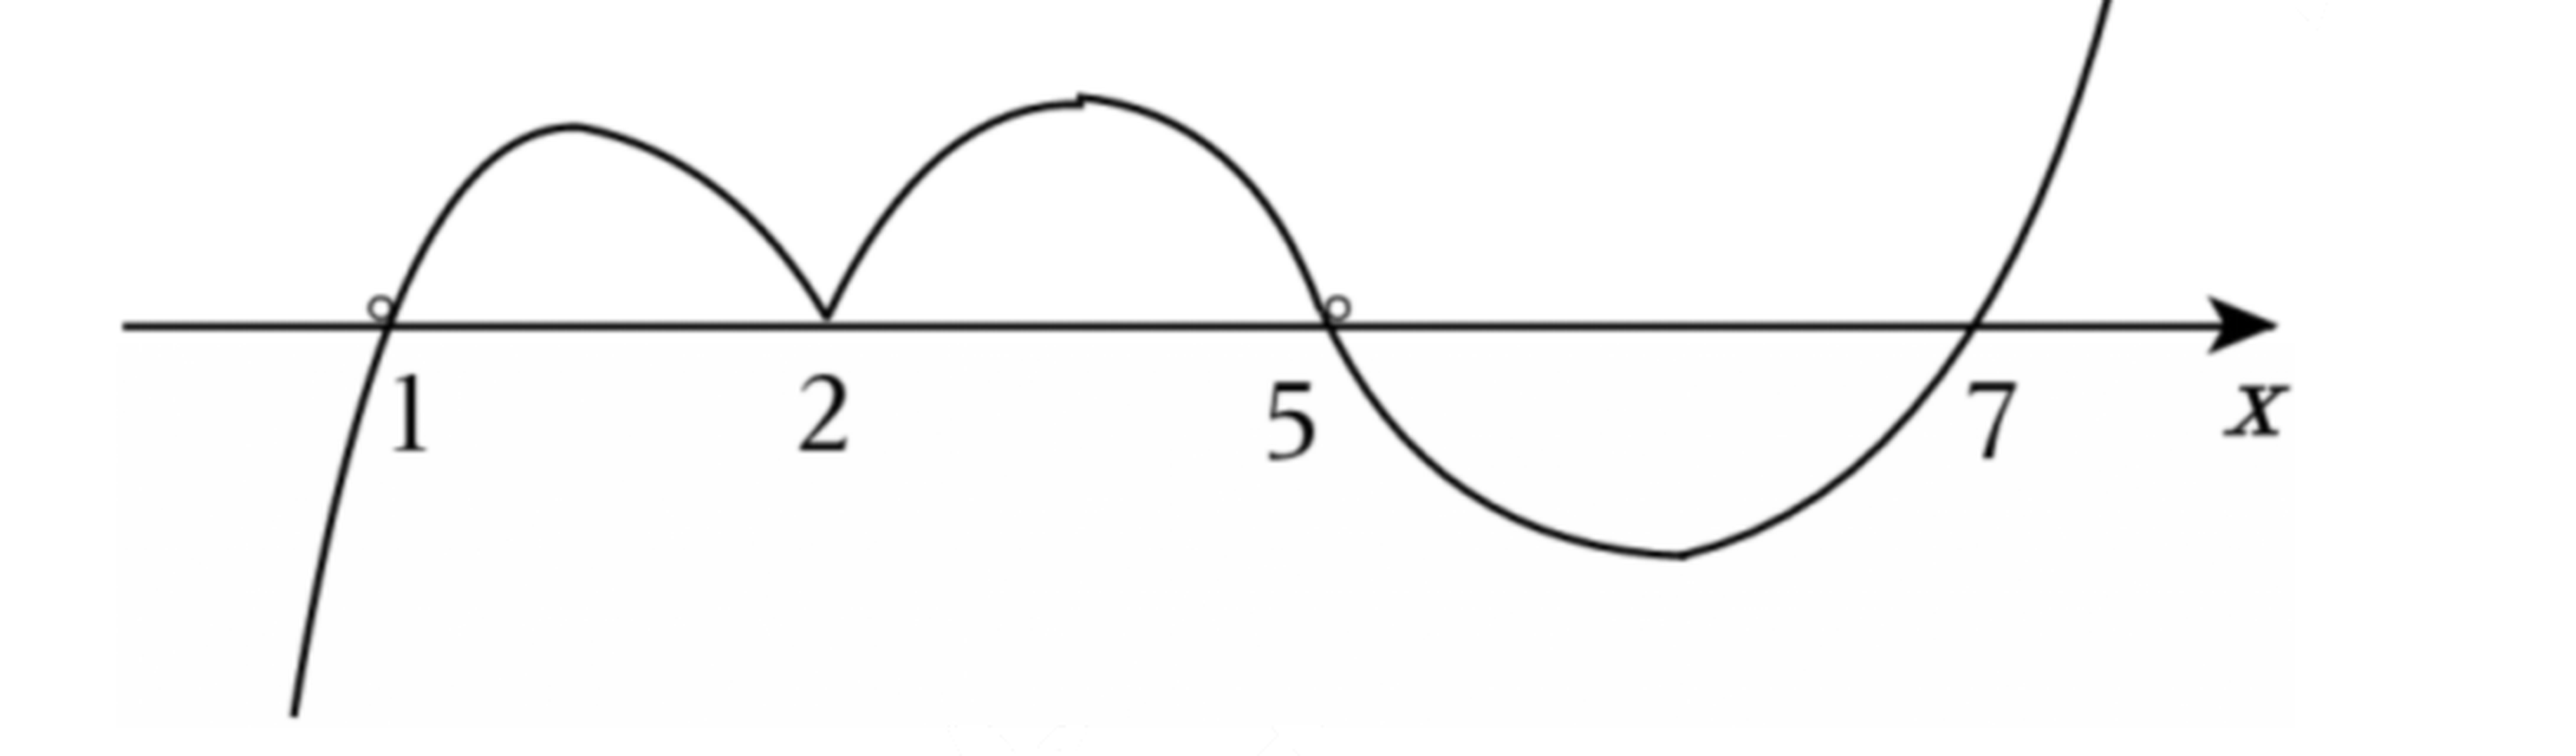
\includegraphics[width=0.62\textwidth]{figures/gao145_q16_a7.png}
\end{center}
\step{得不等式的解集为 $\{x\mid x<1\text{ 或 }x=2\text{ 或 }5<x\leqslant7\}$，}
\step{对应的正整数解为 $2$，$6$，$7$，满足题意，故 $A$ 正确，$C$ 错误.}
\step{故选 $A$.}
\solend
\fi

\end{enumerate}

\bigsec{三、解答题}

\begin{enumerate}
\setcounter{enumi}{16}

% 第 17 题：题干在 06 页、解析续至 07 页，按印刷行断，共 7 行；
% "lg(10÷5)" 的除号照录 \div
\item (1) 已知 $a+a^{-1}=6$，求 $a^2+a^{-2}$ 及 $a^{\frac12}-a^{-\frac12}$ 的值；

(2) 已知 $\lg5=a$，$\lg6=b$，用 $a$、$b$ 分别表示 $\lg2$、$\lg3$、$\lg300$ 和 $\log_{12}15$.

\ifanswer
\solbegin
\step{(1) 因为 $a+a^{-1}=6$，}
\step{所以 $a^2+a^{-2}=(a+a^{-1})^2-2\cdot a\cdot a^{-1}=6^2-2=34$，}
\step{因为 $\left(a^{\frac12}-a^{-\frac12}\right)^2=a-2+a^{-1}=6-2=4$，所以 $a^{\frac12}-a^{-\frac12}=\pm2$；}
\step{(2) $\lg2=\lg(10\div5)=\lg10-\lg5=1-a$，}
\step{$\lg3=\lg(6\div2)=\lg6-\lg2=b-(1-a)=a+b-1$，}
\step{$\lg300=\lg(3\times10^2)=\lg3+\lg10^2=a+b-1+2=a+b+1$，}
\step{所以 $\log_{12}15=\dfrac{\lg15}{\lg12}=\dfrac{\lg3+\lg5}{\lg3+\lg2^2}=\dfrac{a+b-1+a}{a+b-1+2(1-a)}=\dfrac{2a+b-1}{b-a+1}$.}
\solend
\fi

% 第 18 题：题干在 07 页、解析续至 08 页（2 问、分类讨论很长），按印刷行断共 25 行；
% 本卷 Q18 用"图像"（Q13/Q14 用"图象"），逐处照录不统一
\item 已知 $f(x)=(m^2-3m+1)x^{m^2-4m-1}$，$y=f(x)$ 为幂函数且在 $(0,+\infty)$ 上是严格减函数.

(1) 求实数 $m$ 的值以及相应的函数表达式；

(2) 若 $y=f(x)$ 的图像关于 $y$ 轴对称，解关于 $x$ 的不等式 $(x+2)^{1-m}<(3x-1)^{1-m}$.

\ifanswer
\solbegin
\step{(1) 由幂函数的定义得 $m^2-3m+1=1$，}
\step{整理得 $m^2-3m=0$，解得 $m=0$ 或 $m=3$，}
\step{由于 $y=f(x)$ 在 $(0,+\infty)$ 上为严格减函数，}
\step{因此幂函数的指数需满足 $m^2-4m-1<0$，}
\step{当 $m=3$ 时，指数为 $3^2-4\times3-1=-4<0$，满足严格递减条件，}
\step{此时函数表达式为 $f(x)=x^{-4}$，}
\step{当 $m=0$ 时，指数为 $0^2-4\times0-1=-1<0$，满足严格递减条件，}
\step{此时函数表达式为 $f(x)=x^{-1}$，}
\step{所以满足条件的实数 $m$ 为 $0$ 或 $3$，}
\step{对应的函数表达式分别为 $f(x)=x^{-1}$、$f(x)=x^{-4}$；}
\step{(2) 函数图像关于 $y$ 轴对称即函数为偶函数，}
\step{对于 $f(x)=x^{-1}=\dfrac1x$，定义域为 $(-\infty,0)\cup(0,+\infty)$，}
\step{满足 $f(-x)=-f(x)$，为奇函数，图像关于原点对称，}
\step{不满足关于 $y$ 轴对称的条件；}
\step{对于 $f(x)=x^{-4}=\dfrac{1}{x^4}$，定义域为 $(-\infty,0)\cup(0,+\infty)$，}
\step{满足 $f(-x)=f(x)$，为偶函数，图像关于 $y$ 轴对称，}
\step{因此符合条件的 $m$ 值为 $3$，}
\step{将 $m=3$ 代入关于 $x$ 的不等式 $(x+2)^{1-m}<(3x-1)^{1-m}$，}
\step{得 $(x+2)^{1-3}<(3x-1)^{1-3}$，即 $(x+2)^{-2}<(3x-1)^{-2}$，}
\step{因为负指数幂的底数不能为 $0$，所以 $x+2\ne0$ 且 $3x-1\ne0$，}
\step{即 $x\ne-2$ 且 $x\ne\dfrac13$，}
\step{不等式可变形为 $\dfrac{1}{(x+2)^2}<\dfrac{1}{(3x-1)^2}$，}
\step{整理得 $(3x-1)^2<(x+2)^2$，即 $8x^2-10x-3<0$，}
\step{解得 $-\dfrac14<x<\dfrac32$，又 $x\ne-2$ 且 $x\ne\dfrac13$，}
\step{所以不等式的解集为 $\left(-\dfrac14,\dfrac13\right)\cup\left(\dfrac13,\dfrac32\right)$.}
\solend
\fi

% 第 19 题：题干在 08 页、解析续至 09 页，按印刷行断，共 14 行；
% 判别式 cases 块内"△=4a²−16a<0"原卷印扁等边三角 \triangle
%（放大 09 页 zz09_delta.png 与 Q12 高 \Delta 并排确认），逐处照录不统一
\item 已知 $f(x)=ax^2+2ax+4$，$a\in\R$.

(1) 若关于 $x$ 的不等式 $f(x)>0$ 在实数集 $\R$ 上恒成立，求实数 $a$ 的取值范围；

(2) 当 $a<0$ 时，解关于 $x$ 的不等式 $f(x)>(a+1)x+5$.

\ifanswer
\solbegin
\step{(1) 由题意得，关于 $x$ 的不等式 $f(x)>0$ 在实数集 $\R$ 上恒成立，}
\step{即 $ax^2+2ax+4>0$ 在实数集 $\R$ 上恒成立，}
\step{当 $a=0$ 时，不等式为 $4>0$ 恒成立，符合题意；}
\step{当 $a\ne0$ 时，则 $\begin{cases}a>0\\\triangle=4a^2-16a<0\end{cases}$，解得 $0<a<4$.}% 判别式原卷印扁等边三角 $\triangle$，照录
\step{综上所述，实数 $a$ 的取值范围为 $[0,4)$.}
\step{(2) $f(x)=ax^2+2ax+4$，}
\step{当 $a<0$ 时，不等式 $f(x)>(a+1)x+5$ 即为 $ax^2+(a-1)x-1>0$，}
\step{即 $(ax-1)(x+1)>0$，即 $\left(x-\dfrac1a\right)(x+1)<0$，}
\step{当 $a<-1$，即 $\dfrac1a>-1$ 时，解得 $-1<x<\dfrac1a$；}
\step{当 $a=-1$，即 $\dfrac1a=-1$ 时，解得 $x\in\varnothing$；}
\step{当 $-1<a<0$，即 $\dfrac1a<-1$ 时，解得 $\dfrac1a<x<-1$.}
\step{综上所述，当 $a<-1$ 时，不等式的解集为 $\left\{x\mid -1<x<\dfrac1a\right\}$；}
\step{当 $a=-1$ 时，不等式的解集为 $\varnothing$；}
\step{当 $-1<a<0$ 时，不等式的解集为 $\left\{x\mid \dfrac1a<x<-1\right\}$.}
\solend
\fi

% 第 20 题：菜园靠墙图为题目配图（三版都出），题干写"如图"；
% 题干在 09 页（含图）、解析续至 10 页，按印刷行断，共 13 行
\needvspace{8cm}
\item 如图，某人计划用篱笆围成一个一边靠墙（墙足够长）的矩形菜园. 设菜园的长为 $x$ 米，宽为 $y$ 米.

\begin{center}
% 矩形菜园靠墙图取 09 页右下，去粉色水印、去色、4× LANCZOS 放大
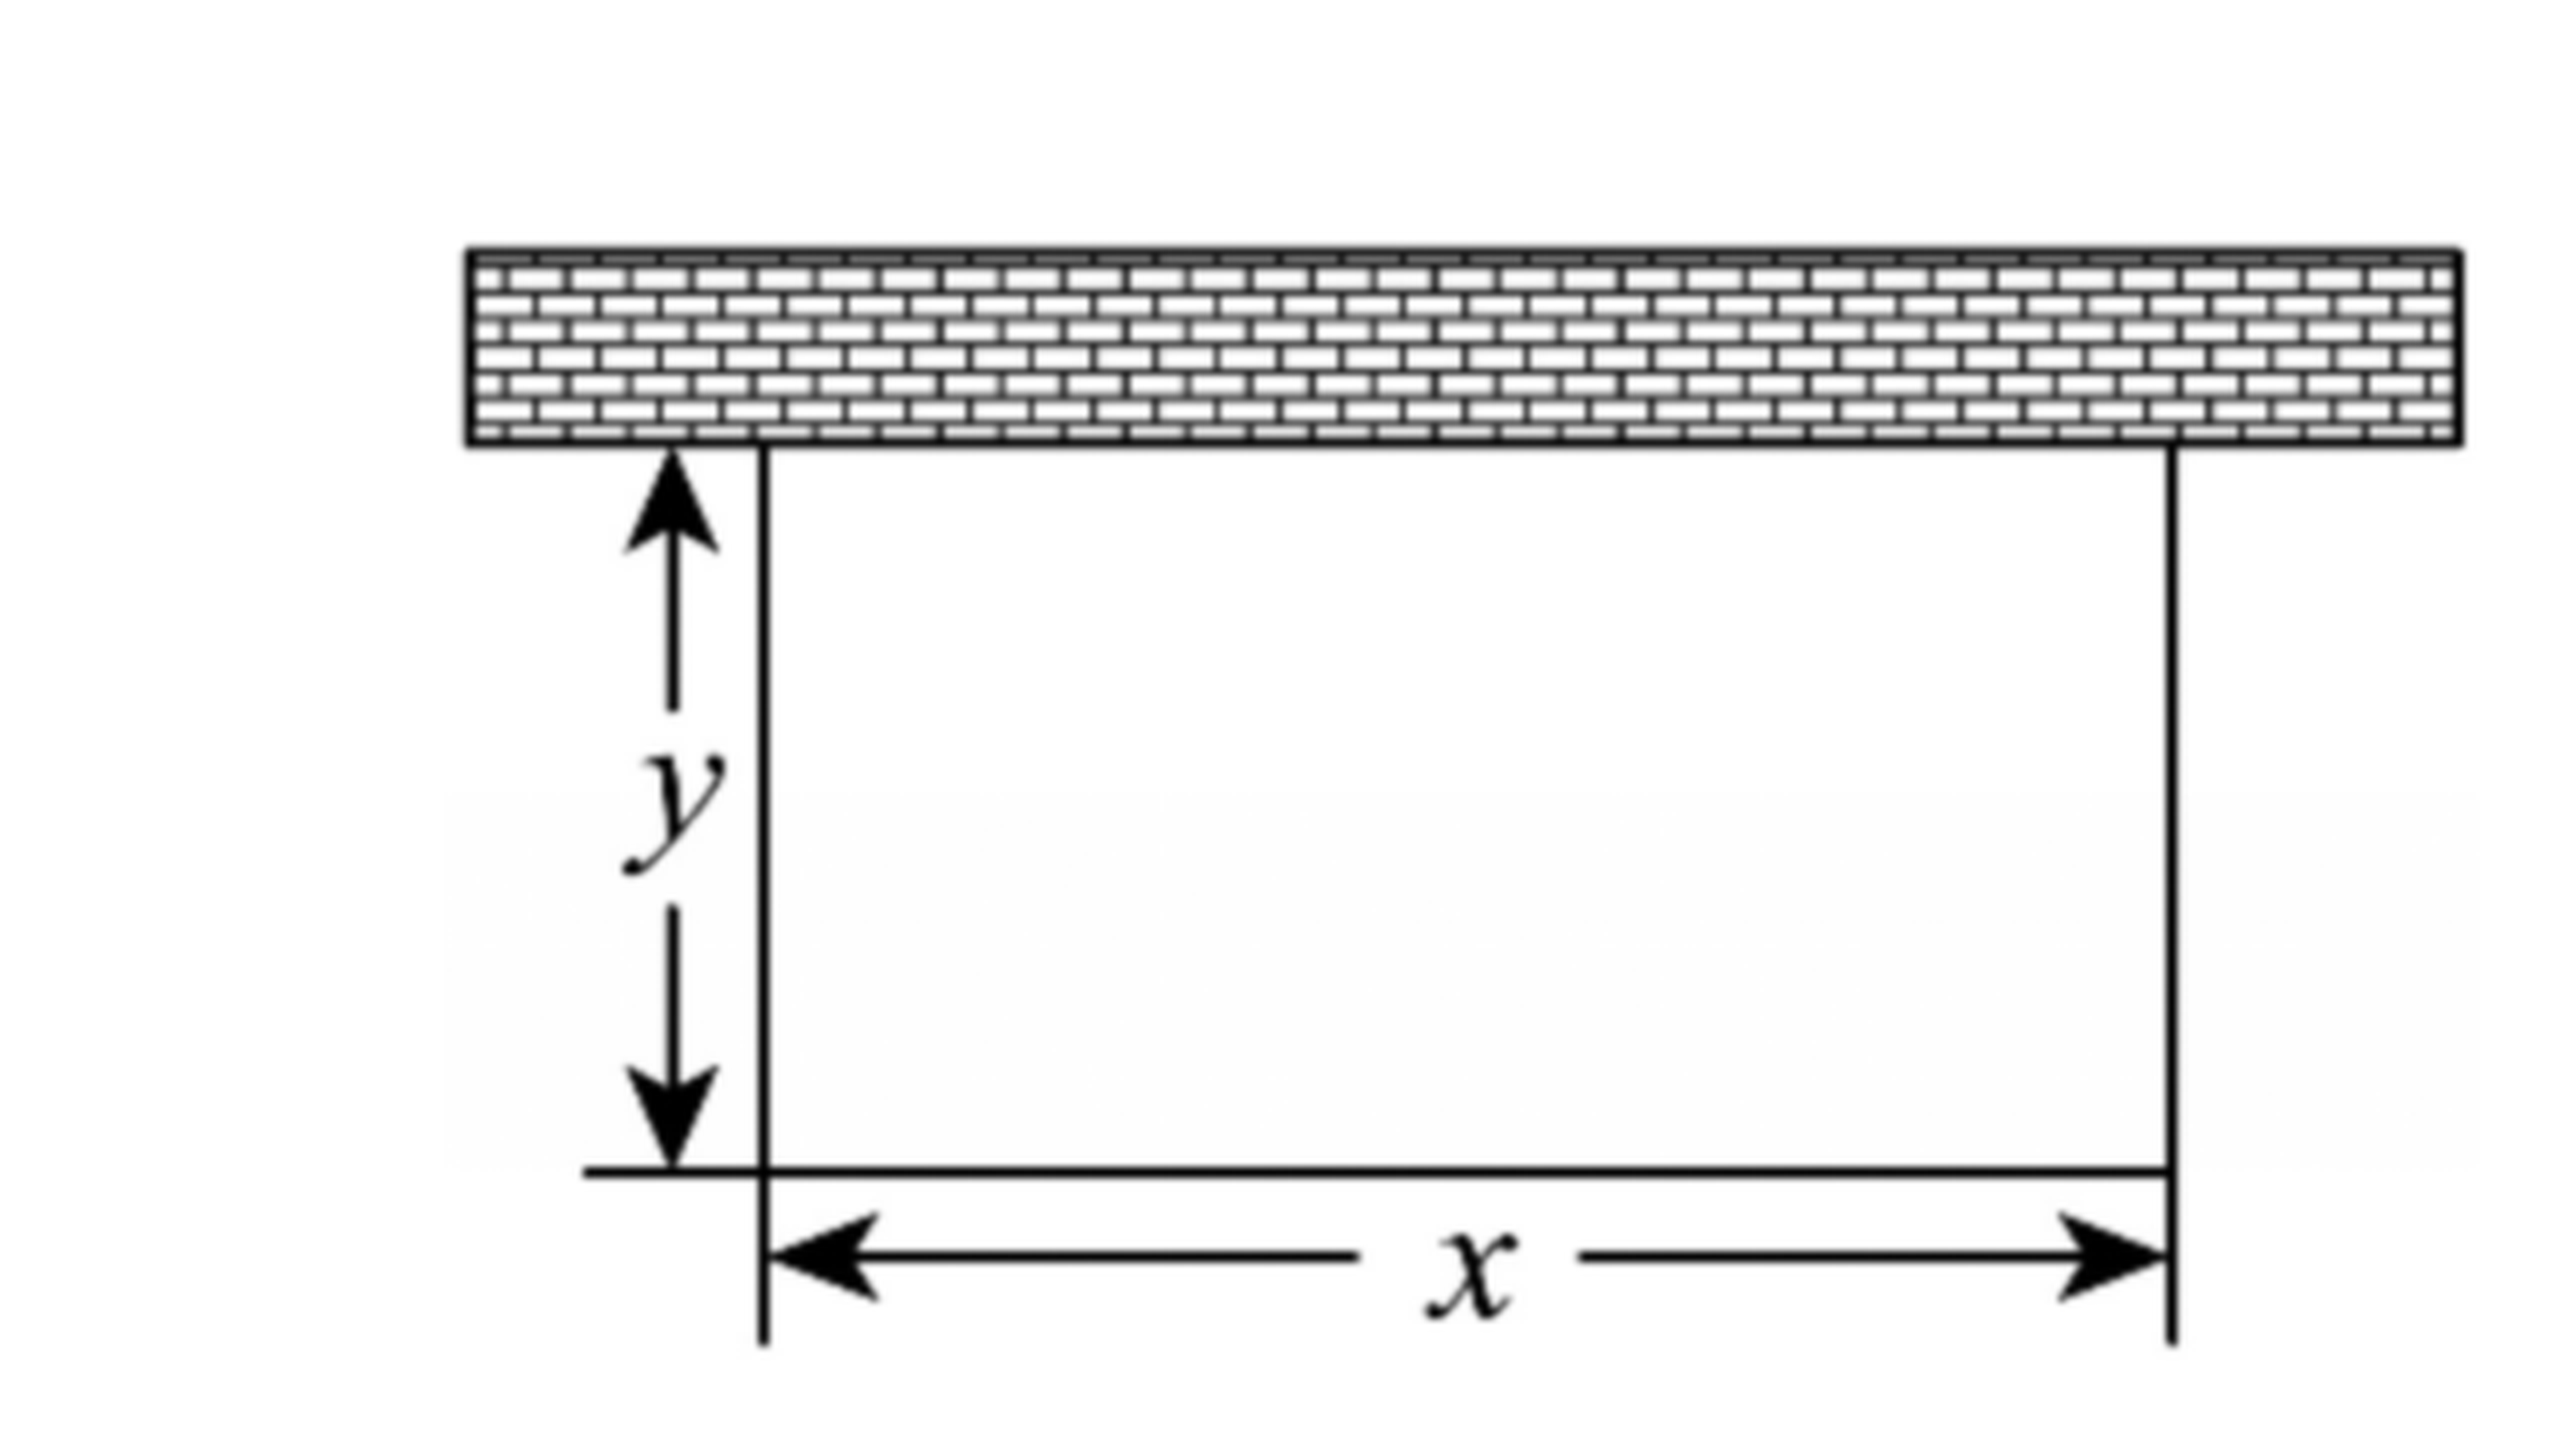
\includegraphics[width=0.55\textwidth]{figures/gao145_q20.png}
\end{center}

(1) 若菜园面积为 72 平方米，则 $x$、$y$ 为何值时，所用篱笆总长最小？

(2) 若 $x$、$y$ 满足 $x+y-xy+63=0$，则菜园面积最小为多少平方米？

\ifanswer
\solbegin
\step{(1) 由题意得，菜园的面积 $S=xy=72$，且 $x>0$，$y>0$，}
\step{所用篱笆总长 $L=x+2y$，}
\step{由基本不等式得 $x+2y\geqslant2\sqrt{x\cdot2y}=2\sqrt{2xy}=2\sqrt{2\times72}=24$，}
\step{当且仅当 $x=2y$ 时取等号，}
\step{联立 $\begin{cases}xy=72\\x=2y\end{cases}$，解得 $\begin{cases}x=12\\y=6\end{cases}$，}
\step{所以当 $x=12$，$y=6$ 时，所用篱笆总长最小；}
\step{(2) 由题意得 $x>0$，$y>0$，且满足 $x+y-xy+63=0$，即 $x+y=xy-63$，}
\step{由基本不等式得 $x+y\geqslant2\sqrt{xy}$，当且仅当 $x=y$ 时取等号，}
\step{所以 $xy-63\geqslant2\sqrt{xy}$. 令 $t=\sqrt{xy}(t>0)$，则 $xy=t^2$，}
\step{上述不等式可化为 $t^2-2t-63\geqslant0$，即 $(t-9)(t+7)\geqslant0$，}
\step{因为 $t>0$，所以 $t+7>0$，故 $t-9\geqslant0$，解得 $t\geqslant9$，所以 $\sqrt{xy}\geqslant9$，}
\step{即 $xy\geqslant81$，当且仅当 $x=y=9$ 时取等号，此时满足 $9+9-81+63=0$，}
\step{所以菜园面积最小为 81 平方米.}
\solend
\fi

% 第 21 题：题干在 10 页、解析续至 11 页（3 问、分类讨论很长），按印刷行断共 22 行；
% 末行"故第 2026 个元素是 2700 之后第一个属于 A 的数，即 2701." 为全卷收尾，
% 无 Q22/Q23、无附加题节；数集 Z/N* 按全稿惯例改 \Z/\N^*
\item 已知集合 $A=\{x\mid x=m^2-n^2$，$m$、$n\in\Z\}$.

(1) 求证：任何奇数 $2k+1(k\in\Z)$ 都是集合 $A$ 中的元素；

(2) 判断偶数 $4k-2(k\in\Z)$ 是否为集合 $A$ 的元素？请说明理由；

(3) 若将集合 $A$ 中的正整数由小到大排列，求出集合 $A$ 中第 2026 个正整数.

\ifanswer
\solbegin
\step{(1) 因为 $x=(k+1)^2-k^2=2k+1(k\in\Z)$，}
\step{所以任何奇数 $2k+1(k\in\Z)$ 都属于集合 $A$；}
\step{(2) 偶数 $4k-2(k\in\Z)$ 不是集合 $A$ 的元素，理由如下：}
\step{由题意得 $x=m^2-n^2=(m-n)(m+n)$，}
\step{当 $m$、$n$ 均为奇数时，设 $m=2k_1+1$，$n=2k_2+1(k_1$、$k_2\in\Z)$，}
\step{则 $m^2-n^2=(2k_1+1)^2-(2k_2+1)^2=(2k_1-2k_2)(2k_1+2k_2+2)$}
\step{$=4(k_1-k_2)(k_1+k_2+1)$，}
\step{因为 $k_1$、$k_2\in\Z$，所以 $k_1-k_2\in\Z$，$k_1+k_2+1\in\Z$，}
\step{从而 $m^2-n^2$ 为 $4$ 的倍数；}
\step{当 $m$、$n$ 均为偶数时，设 $m=2k_1$，$n=2k_2(k_1$、$k_2\in\Z)$，}
\step{$m^2-n^2=4k_1^2-4k_2^2=4(k_1^2-k_2^2)$ 为 $4$ 的倍数；}
\step{当 $m$、$n$ 为一个偶数一个奇数时，不妨设 $m$ 为偶数，$n$ 为奇数，}
\step{设 $m=2k_1$，$n=2k_2+1(k_1$、$k_2\in\Z)$，}
\step{则 $m^2-n^2=4k_1^2-(2k_2+1)^2=4(k_1^2-k_2^2-k_2)-1$ 为奇数.}
\step{无论哪种情况均不满足 $4k-2(k\in\Z)$，}
\step{故偶数 $4k-2(k\in\Z)$ 不是集合 $A$ 的元素；}
\step{(3) 由前两问得，$4$ 的倍数和奇数属于集合 $A$ 中的元素，}
\step{令集合 $A$ 中的正整数元素为 $4k-3$、$4k-1$、$4k(k\in\N^*)$，}
\step{对任意的 $k\in\N^*$，连续的 $4$ 个整数 $4k-3$、$4k-2$、$4k-1$、$4k$ 中}
\step{有三个数 $4k-3$、$4k-1$、$4k$ 都在集合 $A$ 中，}
\step{因为 $2026=3\times675+1$，所以集合 $A$ 中第 $2025$ 个元素为 $4\times675=2700$，}
\step{故第 2026 个元素是 2700 之后第一个属于 $A$ 的数，即 2701.}
\solend
\fi

\end{enumerate}

\end{document}
"
% 紧凑版：xelatex "\def\iscompact{1}% 高一145_市二中学_期中.tex
%   —— 高一上数学"2026-2027 年市二中学高一上期中"（试卷版/答案版/紧凑版）
% 试卷版：xelatex 高一145_市二中学_期中.tex
% 答案版：xelatex "\def\isanswer{1}\input{高一145_市二中学_期中.tex}"
% 紧凑版：xelatex "\def\iscompact{1}\input{高一145_市二中学_期中.tex}"
%
% ① 原始材料：微信公众号"魔都数学加油站"文章，连载"27学年高一145"，原文标题
% "27学年高一145——2026-2027年上海市市二中学高一上期中"；
% 原文链接：https://mp.weixin.qq.com/s/6V-i9KE0GWodC-wmd5z8nQ 。
% 正文为 11 张 PNG 页（01/02/03/08/10/11 为 4762×6735，04/05/06/07/09 为 2560×3620，
% 同一篇各页分辨率不同，逐页按各自分辨率裁图核对，别按预览比例换算裁框）。
% 题目下印【答案】或【解析】，为混合体例讲评版：Q3 只印【答案】、无【解析】，其余
% 18 题印【解析】。题目、解析均据原图转录；卷面粉红色水印"魔都数学加油站"及
% 公众号页脚未录入。
% 全卷插图情况（逐页通读 11 页确认，题干写"如图"处均配有图）：
%   · Q14 韦恩图（05 页右侧，全集 U 矩形＋两圆 M/N＋白色交集、灰色阴影＋U/M/N 标注）：
%     题目配图（选择题选项旁），三版都出，裁自 05 页去水印去色 4× 放大存
%     figures/gao145_q14.png；
%   · Q16 两幅数轴标根波浪曲线（06 页，a=3 与 a=7 各一幅，标根法画
%     (x-1)(x-2)^2(x-5)(x-a)≤0 的符号曲线）：【解析】内的配图，仅答案版出，
%     裁 figures/gao145_q16_a3.png / figures/gao145_q16_a7.png（或合并一张），
%     放在答案版条件块内 \solbegin 的 \step 之间（照 高一73 第 16 题成例）；
%   · Q20 矩形菜园靠墙图（09 页右下，灰色砖墙＋矩形菜园＋x/y 标注＋箭头）：
%     题目配图，三版都出，裁自 09 页去水印去色 4× 放大存 figures/gao145_q20.png；
%   其余各页逐页确认无其它题目配图、无表格、亦无"题干写如图而源码漏图"一处。
%
% 卷首标题：原卷印作"2026-2027 年市二中学高一上期中"，年份区间按全稿惯例排 en dash；
% 原卷卷面未印副标题，本稿按同期中卷（高一140／141／143／144）知识模块口径补出
% "集合与常用逻辑用语、不等式、函数"。
%
% 题号体例：本卷共 19 题——一、填空题 3—12（10 题）、二、选择题 13—16（4 题）、
% 三、解答题 17—21（5 题）。三节分别 \setcounter{enumi}{2}／{12}／{16}。
% 原卷从第 3 题起、无第 1、2 题，本稿保留原题号；全卷无附加题节。
%
% ② 与原卷的排版差异：
%   ① 原文从第 3 题起，本稿保留原题号；共 19 题三节；
%   ② 混合体例：原卷 Q3 只印【答案】、无【解析】（"第一步应假设___。
%      【答案】x≤2 或 y≤2"），按 高一140 第 5 题成例提 \ans{}、不补造解析；
%      其余 18 题印【解析】，用 \solbegin…\solend，选择题答案在解析末句"故选 X"
%      （Q13 选 B、Q14 选 D、Q15 选 D、Q16 选 A，逐个放大原图核实）、
%      题干括号 \mbox{（\quad）} 留空、不另提 \ans{}；填空／解答答案落在解析里；
%      答案版【答案】/【解析】标记数 = 19（1 个 \ans ＋ 18 个 \solbegin）= 全卷题数；
%   ③ 原卷卷面未印副标题，本稿按知识模块口径补出；
%   ④ 原卷填空横线按全稿惯例排 \blankline[4.4em]；选择题括号排 \mbox{（\quad）}、
%      选项段前按惯例加 \keepwithprev；解答题不留作答区、不加 \anspace
%      （原卷为讲评版，与 129／131／132／133／136／140／141／143／144 同）；
%   ⑤ 数集：Q9"a、b∈R"、Q12"a∈R"、Q21"m、n∈Z""k∈Z""k∈N*"等原卷印
%      斜体或黑板粗体 R/Z/N，按全稿惯例统一改 \R／\Z／\N^*；绝对值排 \lvert…\rvert，
%      集合描述竖线排 \mid；不等号按全稿惯例排 \leqslant／\geqslant；
%      补集照原卷上划线排 \overline{M}／\overline{N}（Q14 选项 B/C/D 逐处核）；
%      空集记号 \varnothing；\subset（单线⊂）与 \subseteq（带下划线⊆）逐处照录不统一；
%   ⑥ 子题标号 (1)(2)(3) 原卷印半角括号照录；圈数字进数学式用 \text{①}（否则 FONTCHK 挂）；
%      \left…\right 不得拆到不同 $…$ 组；cases 块整体算一个印刷行；
%   ⑦ 题干／解析中的中文弯引号按原卷照录（Q3"若 x+y>4，则 x>2 且 y>2"、
%      Q11"a₁/a₂=b₁/b₂""M=N"、选填"充分非必要""必要非充分""充要""既非充分也非必要"
%      等，含引号内空格），注释内一律 ASCII 引号；数学式内 CJK 用 \text{}；
%   ⑧ 半角逗号在数学组之间是全稿惯例、非笔误（如 Q5"x₁+x₂=6，x₁x₂=√3"、
%      Q7"a>1，b>1"、指数／对数式内逗号），逐处照录别改全角；行末西文句点照录为
%      ASCII `.`；行中全角逗号／顿号照录；
%   ⑨ "图像／图象"逐处照录不统一（Q18"图像关于 y 轴对称"等，核全卷）；
%   ⑩ 判别式 Δ/△ 混用是照录项：Q12 解析"Δ=a²−4a²(2a−3)>0"、
%      Q19 解析"Δ=4a²−16a<0"等，放大原图判断是高 \Delta（等腰偏高、高>宽）
%      还是扁 \triangle，逐处照录不得统一（参照 高一142／144 头注④口径）；
%   ⑪ 一条 \step = 原卷解析的一个印刷行，cases 块整体算一个印刷行；别把原卷折行
%      并起来、别把一行拆多条。Q6 分段讨论、Q12 三个 cases 条件组、Q16 数轴标根、
%      Q18／Q19 分类讨论、Q21 三问均按印刷行逐条断，不丢行；
%   ⑫ Q14 韦恩图为"题干＋选项＋图"整块，加 \needvspace 守卫推走（守卫放 \item 之前，
%      见 高一140 Q14、高一144 Q17 成例与切页审计 B 类坑）；Q20 菜园图同理；
%      三版切页审计均"合计异常：无"；
%   ⑬ 跨页续印按题合并：Q3/4/5/6 在 01 页（Q6 解析续 02 页顶）；Q7/8/9/10 在 02 页
%      （Q10 解析续 03 页）；Q11/12 在 03 页（Q12 解析续 04 页，很长）；
%      Q13 在 04 页末、解析在 05 页顶；Q14/15/16 在 05 页（Q16 解析续 06 页含两幅数轴图）；
%      Q17 在 06 页、解析续 07 页；Q18 在 07 页、解析续 08 页；Q19 在 08 页、解析续 09 页；
%      Q20 在 09 页（含菜园图）、解析续 10 页；Q21 在 10 页、解析续 11 页
%      （末页收尾"故第 2026 个元素是 2700 之后第一个属于 A 的数，即 2701."、
%      无 Q22/Q23、无附加题节）。本稿按题连排，不丢行、不并折行；
%   ⑭ 原卷解析内若有红色"法一／法二"之类小标题，按全稿惯例排 \stepm{标签}{…}
%      （黑体着色、不引入红色、不改 common.sty），头注注明；水印"魔都数学加油站"
%      红色不录入。
%
% ③ 行数复核：一条 \step／\stepm = 原卷解析的一个印刷行，cases 块作一个印刷行计。
%   逐题数（主会话逐页核对定稿）：Q3：0（只印【答案】、提 \ans{}，不计入 \step 账）；
%   Q4：3；Q5：2；Q6：10；Q7：3；Q8：3；Q9：2；Q10：7；Q11：4；Q12：12；
%   Q13：2；Q14：2；Q15：4；Q16：9；Q17：7；Q18：25；Q19：14；Q20：13；Q21：22。
%   合计 144 条 \step（本卷无 \stepm：解析内无红色"法一／法二"类小标题），
%   与原卷逐题印刷行相等。全卷 18 题设 \solbegin…\solend ＋ Q3 一处 \ans{}，
%   答案版【答案】/【解析】标记数 = 19 = 全卷题数。
%
% ④ 判别式／子集符号结论（逐处放大原图照录、不得统一，主会话像素级复核）：
%   判别式全卷 2 处、两形混用逐处照录不统一（参照 高一142／144 头注④口径）：
%     · Q12 解析 cases 块"Δ=a²−4a²(2a−3)>0" 原卷印等腰偏高粗三角（高>宽），
%       照录 \Delta（放大 04 页 /tmp/gao145s2/main_q12_delta.png 确认）；
%     · Q19 解析 cases 块"△=4a²−16a<0" 原卷印扁等边空心三角（宽≈高、细线），
%       照录 \triangle（放大 09 页 /tmp/gao145s2/main_q19_delta.png 确认）。
%   子集／补集：Q14 选项 A `M\cup N`、B `M\cap\overline{N}`（上划线只在 N 上）、
%   C `\overline{M\cup N}`（罩整个 M∪N）、D `\overline{M\cap N}`（罩整个 M∩N，
%   非 \overline{M}\cap N；放大 05 页 /tmp/gao145s2/main_q14_opts.png 确认），
%   阴影为灰色区域＝全集减白色交集，答案 D，照录 \overline{M\cap N}；
%   全集卷无 \subset／\subseteq 混用（本卷集合题用 \cup／\cap／\overline{}）；
%   空集 \varnothing（Q19 解析 x∈\varnothing）；数集 \R／\Z／\N^* 归一见 ② ⑤。
%
% ⑤ 存疑照录（放大原图确认，照录未改、正文对应处另有 % 注）：
%   1. Q3 题干"若 x+y>4，则 x>2 且 y>2" 后"时"前留一空格、弯引号内空格照录；
%      该卷混合体例（Q3 只印【答案】、提 \ans{}）见 ② ②。
%   2. Q4／Q5 解析中的"1，3，5 和 6"、"x₁+x₂=6,x₁x₂=√3" 等半角／全角逗号
%      逐处照原卷（放大 01 页确认），数学式内半角逗号为全稿惯例、非笔误。
%   3. Q14 选项 D 上划线罩住整个 M∩N（而非仅罩 M），照录 \overline{M\cap N}。
%   4. Q12 判别式高 \Delta 与 Q19 判别式扁 \triangle 两形混用，逐处照录不统一（见 ④）。
%   全卷除此 4 类外未发现其它笔误／自相矛盾处。
%
% ⑥ 跨页续印按题合并说明：见 ② ⑬。
%
\documentclass[a4paper,11pt]{article}
\usepackage{common}

\begin{document}

\examtitlest[3]{2026--2027 年市二中学高一上期中}{集合与常用逻辑用语、不等式、函数}

\bigsec{一、填空题}

\begin{enumerate}
\setcounter{enumi}{2}

% 第 3 题：原卷只印【答案】、无【解析】（放大 01 页确认），按 高一140 第 5 题成例
% 提 \ans{}、不补造解析；题干中文弯引号与"时"前空格照录
\item 用反证法证明命题：“若 $x+y>4$，则 $x>2$ 且 $y>2$” 时，第一步应假设\blankline[4.4em].

\ifanswer
\ans{$x\leqslant2$ 或 $y\leqslant2$}
\fi

% === Q4 ===
\item 设集合 $M$ 满足 $\{1,3,5,6\}\cup M=\{1,2,3,4,5,6\}$，则满足条件的所有 $M$ 的个数为\blankline[4.4em].

\ifanswer
\solbegin
\step{集合 $M$ 满足 $\{1,3,5,6\}\cup M=\{1,2,3,4,5,6\}$，}
\step{则 $M$ 中必含有 $2$ 和 $4$，$1$，$3$，$5$ 和 $6$ 可以选也可不选，}
\step{则满足条件的所有 $M$ 的数目相当于集合 $\{1,3,5,6\}$ 的子集的个数 $2^4=16$.}
\solend
\fi

% === Q5 ===
\item 已知方程 $x^2-6x+\sqrt3=0$ 的两根为 $x_1$ 和 $x_2$，则 $(x_1-x_2)^2=$\blankline[4.4em].

\ifanswer
\solbegin
\step{因为方程 $x^2-6x+\sqrt3=0$ 的两根为 $x_1$ 和 $x_2$，所以 $x_1+x_2=6,x_1x_2=\sqrt3$，}% 数学式内半角逗号为全稿惯例，照录
\step{所以 $(x_1-x_2)^2=(x_1+x_2)^2-4x_1x_2=36-4\sqrt3$.}
\solend
\fi

% 第 6 题：题干在 01 页，解析续至 02 页顶（末 2 行），按印刷行逐条断，共 10 行
\item 不等式 $\lvert x-2026\rvert+\lvert x-2029\rvert>3$ 的解集是\blankline[4.4em].

\ifanswer
\solbegin
\step{当 $x<2026$ 时，$x-2026<0$，$x-2029<0$，}
\step{原不等式可化为 $(2026-x)+(2029-x)>3$，解得 $x<2026$，}
\step{故此时，不等式的解为 $x<2026$；}
\step{当 $2026\leqslant x\leqslant2029$ 时，$x-2026\geqslant0$，$x-2029\leqslant0$，}
\step{原不等式可化为 $(x-2026)+(2029-x)>3$，即 $3>3$，显然不成立，}
\step{故此时，不等式无解；}
\step{当 $x>2029$ 时，$x-2026>0$，$x-2029>0$，}
\step{原不等式可化为 $(x-2026)+(x-2029)>3$，解得 $x>2029$，}
\step{故此时，不等式的解为 $x>2029$.}
\step{综上，原不等式的解集为 $(-\infty,2026)\cup(2029,+\infty)$.}
\solend
\fi

% === Q7 ===
\item 已知 $a>1$，$b>1$，若 $\log_a b+\log_b a=2$，且 $ab=2$，则 $\log_2(a+b)=$\blankline[4.4em].

\ifanswer
\solbegin
\step{由 $\log_a b+\log_b a=2$，$a>1$，$b>1$，得 $\log_a b+\dfrac{1}{\log_a b}=2$，}
\step{即 $(\log_a b)^2-2\log_a b+1=0$，则 $(\log_a b-1)^2=0$，解得 $\log_a b=1$，即 $a=b$，}
\step{又 $ab=2$，所以 $a=b=\sqrt2$，所以 $\log_2(a+b)=\log_2 2\sqrt2=\log_2 2^{\frac32}=\dfrac32$.}
\solend
\fi

% === Q8 ===
\item 已知 $m>0$，$n>0$，且 $m+n=1$，则 $\dfrac1m+\dfrac4n$ 的最小值为\blankline[4.4em].

\ifanswer
\solbegin
\step{由 $m>0$，$n>0$，$m+n=1$，}
\step{则 $\dfrac1m+\dfrac4n=(m+n)\left(\dfrac1m+\dfrac4n\right)=5+\dfrac nm+\dfrac{4m}n\geqslant5+2\sqrt{\dfrac nm\cdot\dfrac{4m}n}=9$，}
\step{当且仅当 $n=2m=\dfrac23$ 时，上式取得等号，故最小值为 $9$.}
\solend
\fi

% === Q9 ===
\item 已知 $a$、$b\in\R$，且 $3a+2b=1$，则 $8^a+4^b$ 最小值为\blankline[4.4em].

\ifanswer
\solbegin
\step{因为 $3a+2b=1$，所以 $8^a+4^b=2^{3a}+2^{2b}\geqslant2\sqrt{2^{3a+2b}}=2\sqrt2$，}
\step{当且仅当 $3a=2b$ 时取等号，故最小值为 $2\sqrt2$.}
\solend
\fi

% 第 10 题：题干在 02 页、解析续至 03 页顶，按印刷行断，共 7 行
\item 已知关于 $x$ 的不等式 $ax^2+bx+c>0$ 的解集为 $\{x\mid 1<x<2\}$，则关于 $x$ 的不等式 $bx^2-ax+c<0$ 的解集为\blankline[4.4em].

\ifanswer
\solbegin
\step{已知关于 $x$ 的不等式 $ax^2+bx+c>0$ 的解集为 $\{x\mid 1<x<2\}$，}
\step{由解集为 $1<x<2$ 且二次函数在两根之间为正，得 $a<0$，两个根为 $1$，$2$，}
\step{所以 $ax^2+bx+c=a(x-1)(x-2)=ax^2-3ax+2a$，}
\step{比较系数得 $b=-3a$，$c=2a$.}
\step{于是 $bx^2-ax+c=-3ax^2-ax+2a=-a(3x-2)(x+1)$，}
\step{$a<0$，故 $bx^2-ax+c<0$ 等价于 $(3x-2)(x+1)<0$，解得 $-1<x<\dfrac23$，}
\step{故 $bx^2-ax+c<0$ 的解集为 $\left\{x\mid -1<x<\dfrac23\right\}$.}
\solend
\fi

% 第 11 题：题干引号内空格照录（放大 03 页确认），四组选填引号亦同；
% 结论"故为必要非充分条件"照录，解析共 4 个印刷行
\item 设 $a_1$、$b_1$、$a_2$、$b_2$ 均为非零实数，不等式 $a_1x+b_1>0$ 和 $a_2x+b_2>0$ 的解集分别为集合 $M$、$N$，那么 “ $\dfrac{a_1}{a_2}=\dfrac{b_1}{b_2}$ ” 是 “ $M=N$ ” 的\blankline[4.4em]条件（选填 “ 充分非必要 ”、“ 必要非充分 ”、“ 充要 ” 和 “ 既非充分也非必要 ”）.

\ifanswer
\solbegin
\step{当 $a_1=b_1=1$，$a_2=b_2=-1$ 时，满足 $\dfrac{a_1}{a_2}=\dfrac{b_1}{b_2}$，}
\step{但是 $M=N$ 不成立，即充分性不成立；}
\step{若 $M=N$ 时，$\dfrac{a_1}{a_2}=\dfrac{b_1}{b_2}$ 一定成立，即必要性成立.}
\step{故为必要非充分条件.}
\solend
\fi

% 第 12 题：题干在 03 页、解析续至 04 页（很长，含 3 个 cases 条件组），
% 按印刷行逐条断共 12 行；cases 块整体算一个印刷行
\item 已知 $f(x)=\dfrac{ax+3}{x-2}$（常数 $a\in\R$）. 函数 $y=f(x)$ 在区间 $[3,+\infty)$ 上是严格减函数，且函数值不恒为负. 若关于 $x$ 的方程 $f(x)=\dfrac{a}{ax-1}$ 有两个不相等的实数根 $x_1$ 和 $x_2$，则 $a$ 的取值范围是\blankline[4.4em].

\ifanswer
\solbegin
\step{$f(x)=\dfrac{ax+3}{x-2}=a+\dfrac{3+2a}{x-2}$，定义域 $(-\infty,2)\cup(2,+\infty)$，}
\step{由于 $y=f(x)$ 在区间 $[3,+\infty)$ 上是严格减函数，且函数值不恒为负，}
\step{所以 $\begin{cases}3+2a>0\\a+\dfrac{3+2a}{3-2}\geqslant0\end{cases}\Rightarrow a\geqslant-1$，}
\step{若关于 $x$ 的方程 $f(x)=\dfrac{a}{ax-1}$ 有两个不相等的实数根 $x_1$ 和 $x_2$，}
\step{则 $\dfrac{ax+3}{x-2}=\dfrac{a}{ax-1}$，即 $(ax+3)(ax-1)=a(x-2)$，$x\ne2$ 且 $ax-1\ne0$，}
\step{当 $a\ne0$ 且 $a\geqslant-1$ 时，$(ax+3)(ax-1)=a(x-2)$，$x\ne2$ 且 $ax-1\ne0$，}
\step{可化为 $\begin{cases}a^2x^2+ax+2a-3=0\\x\ne2,x\ne\dfrac1a\end{cases}$，}
\step{要使方程有两个不相等的实数根 $x_1$ 和 $x_2$，}
\step{则 $\begin{cases}\Delta=a^2-4a^2(2a-3)>0\\a\geqslant-1\text{且}a\ne0\\4a^2+2a+2a-3\ne0\\a^2\cdot\dfrac1{a^2}+a\cdot\dfrac1a+2a-3\ne0\end{cases}\Rightarrow\begin{cases}a<\dfrac{13}{8}\\a\geqslant-1\text{且}a\ne0\\a\ne\dfrac12\text{且}a\ne-\dfrac32\\a\ne\dfrac12\end{cases}$，}% 判别式原卷印等腰偏高三角 $\Delta$，照录（放大 04 页 zz04_delta.png 确认）
\step{得 $-1\leqslant a<\dfrac{13}{8}$ 且 $a\ne0,a\ne\dfrac12$；}
\step{当 $a=0$ 时，方程无解；}
\step{所以 $a$ 的取值范围是 $[-1,0)\cup\left(0,\dfrac12\right)\cup\left(\dfrac12,\dfrac{13}{8}\right)$.}
\solend
\fi

\end{enumerate}

\bigsec{二、选择题}

\begin{enumerate}
\setcounter{enumi}{12}

% 第 13 题：题干在 04 页末、解析在 05 页顶；"图象"照录（本卷 Q13、Q14 用"图象"）
\item 已知幂函数 $f(x)$ 的图象过点 $\left(7,\dfrac{1}{\sqrt7}\right)$，则 $f(x)=$\mbox{（\quad）}

\keepwithprev
A. $x^{-2}$\qquad B. $x^{-\frac12}$\qquad C. $x^{\frac12}$\qquad D. $x^2$

\ifanswer
\solbegin
\step{设幂函数 $f(x)=x^\alpha(\alpha\in\R)$，因为幂函数的图象过点 $\left(7,\dfrac{1}{\sqrt7}\right)$，}
\step{所以 $7^\alpha=\dfrac{1}{\sqrt7}=7^{-\frac12}$，所以 $\alpha=-\dfrac12$，故 $f(x)=x^{-\frac12}$. 故选 $B$.}
\solend
\fi

% 第 14 题：韦恩图为题目配图（三版都出），"题干＋选项＋图"整块，needvspace
% 守卫放在 \item 之前（Q14 为选择题节内第二题，不会让节标题孤落页末）；
% D 选项上划线罩住整个 M∩N（放大 05 页 zz05_q14D.png 确认，非 \overline{M}\cap N）
\needvspace{9cm}
\item 已知全集 $U$ 和集合 $M$、$N$，用集合语言表示图中的阴影部分，正确的是\mbox{（\quad）}

\keepwithprev
A. $M\cup N$\qquad B. $M\cap\overline{N}$\qquad C. $\overline{M\cup N}$\qquad D. $\overline{M\cap N}$

\begin{center}
% 韦恩图取 05 页右侧，去粉色水印、去色、4× LANCZOS 放大
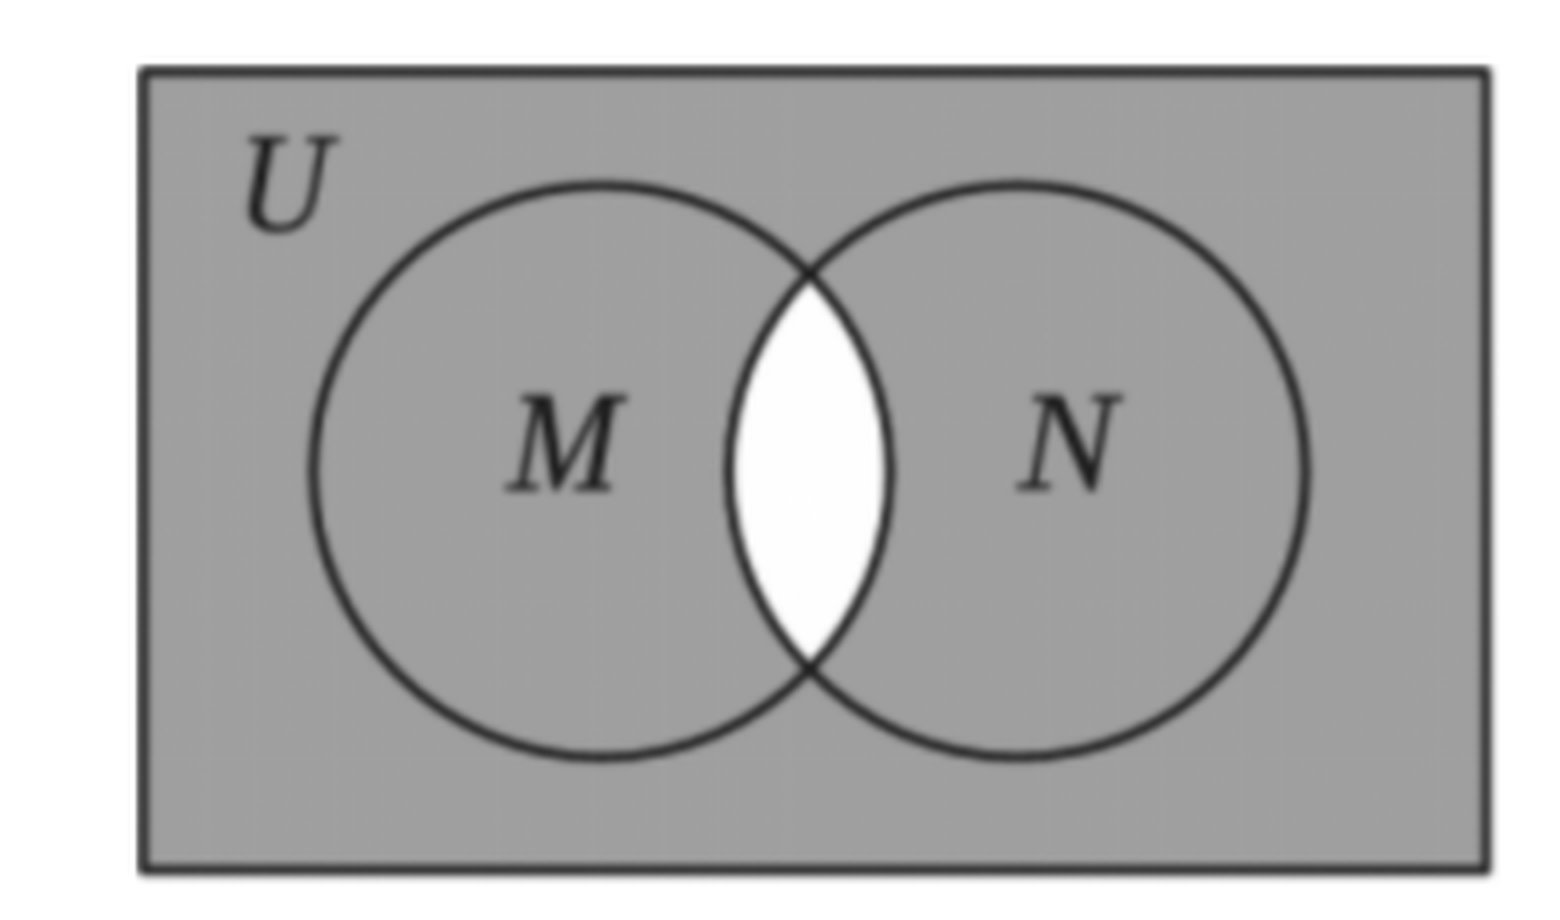
\includegraphics[width=0.40\textwidth]{figures/gao145_q14.png}
\end{center}

\ifanswer
\solbegin
\step{由韦恩图得图中白色区域为集合 $M\cap N$，所以阴影部分表示的集合为 $\overline{M\cap N}$.}
\step{故选 $D$.}
\solend
\fi

% === Q15 ===
\item 已知 $x>-2$，则 $x+\dfrac{1}{x+2}$ 的最小值为\mbox{（\quad）}

\keepwithprev
A. 3\qquad B. 2\qquad C. 1\qquad D. 0

\ifanswer
\solbegin
\step{$x>-2$，则 $x+2>0$，}
\step{所以 $x+\dfrac{1}{x+2}=(x+2)+\dfrac{1}{x+2}-2\geqslant2\sqrt{(x+2)\cdot\dfrac{1}{x+2}}-2=0$，}
\step{当且仅当 $x+2=\dfrac{1}{x+2}$，即 $x=-1$ 时取等号，所以 $x+\dfrac{1}{x+2}$ 的最小值为 $0$.}
\step{故选 $D$.}
\solend
\fi

% 第 16 题：题干在 05 页、解析续至 06 页；两幅数轴标根波浪曲线是【解析】内配图，
% 仅答案版出，放在答案版条件块内 \solbegin 的 \step 之间（照 高一73 第 16 题成例）
\item 关于 $x$ 的不等式 $\dfrac{(x-a)(x-2)^2}{(x-1)(x-5)}\leqslant0$ 的解集中恰有 3 个正整数，则实数 $a$ 的取值范围是\mbox{（\quad）}

\keepwithprev
A. $(-\infty,3]\cup[7,8)$\qquad B. $(-\infty,3)\cup[7,8)$\qquad C. $(-\infty,3]\cup(7,8]$\qquad D. $(-\infty,3)\cup(7,8]$

\ifanswer
\solbegin
\step{由题意，不等式 $\dfrac{(x-a)(x-2)^2}{(x-1)(x-5)}\leqslant0$，}
\step{可化为 $\begin{cases}(x-1)(x-2)^2(x-5)(x-a)\leqslant0\\x\ne1\text{且}x\ne5\end{cases}$，由数轴标根法，}
\step{当 $a=3$ 时，}
\begin{center}
% a=3 数轴标根图取 06 页，去粉色水印、去色、4× LANCZOS 放大；仅答案版出
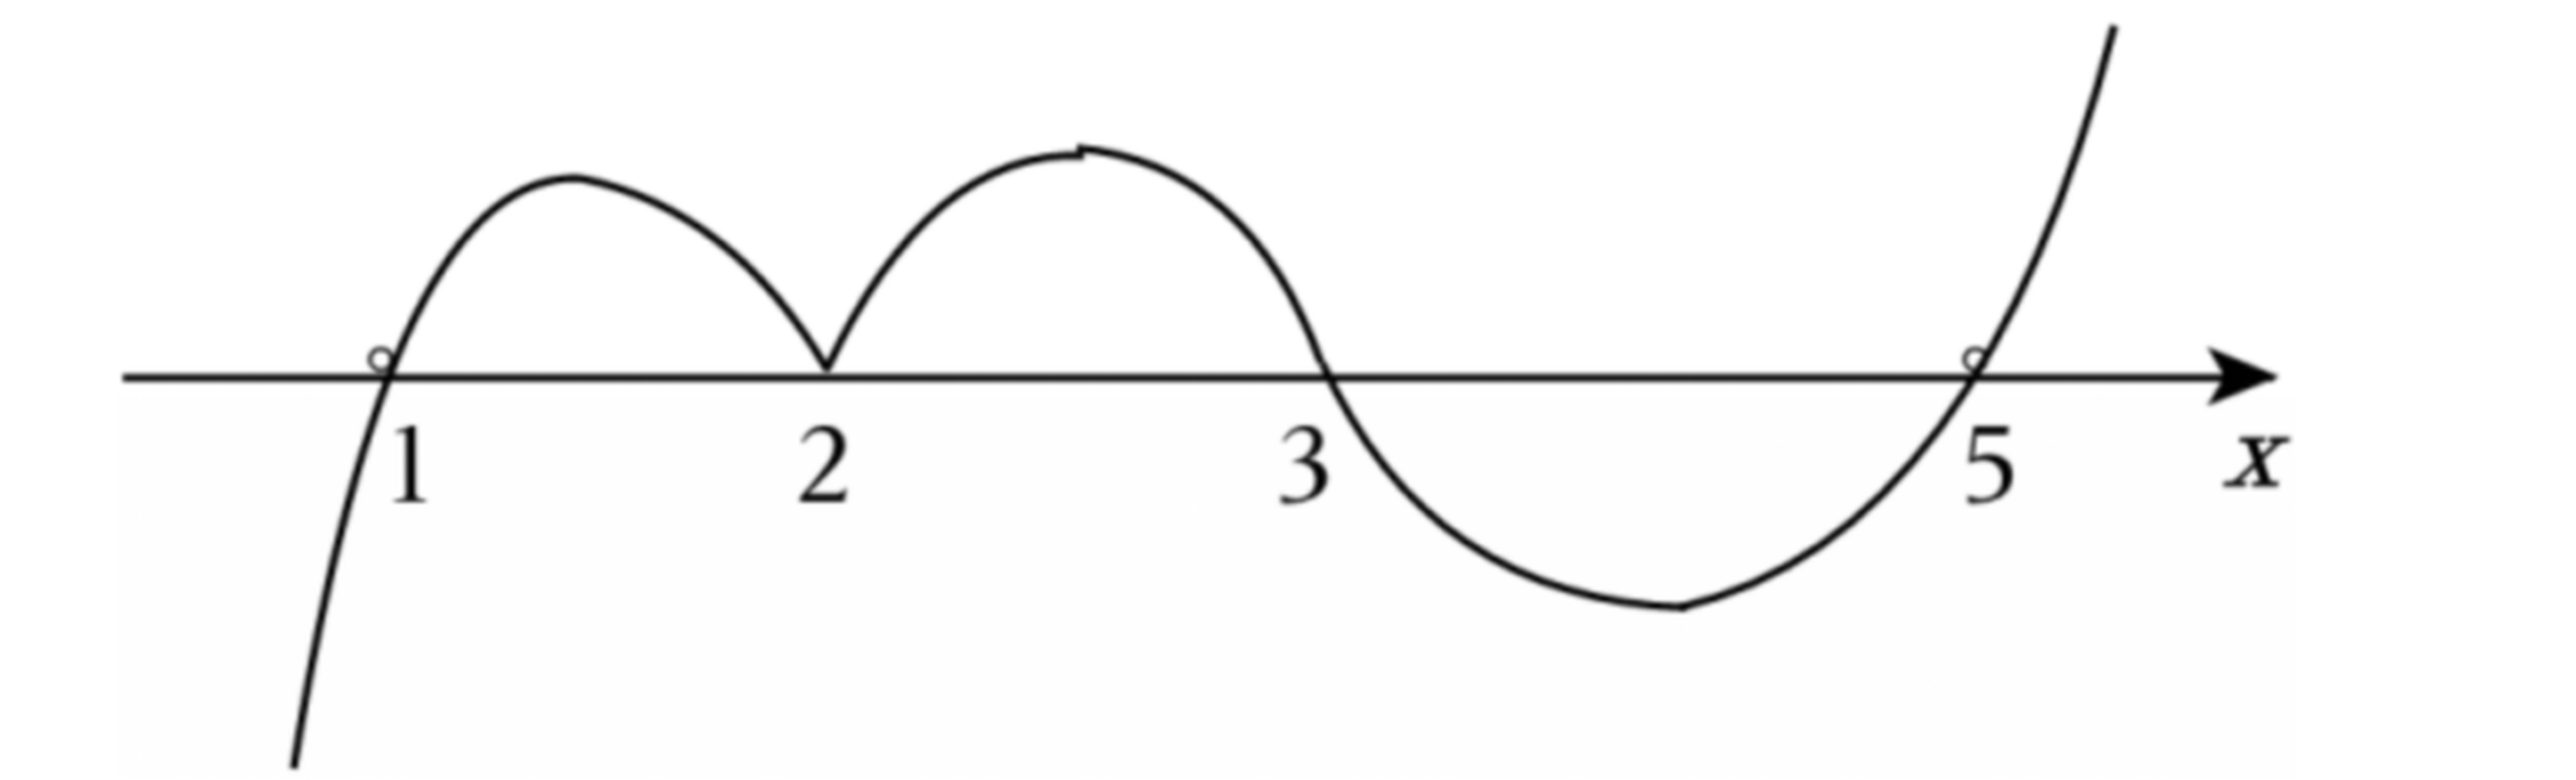
\includegraphics[width=0.62\textwidth]{figures/gao145_q16_a3.png}
\end{center}
\step{得不等式的解集为 $\{x\mid x<1\text{ 或 }x=2\text{ 或 }3\leqslant x<5\}$，}
\step{对应的正整数解为 $2$，$3$，$4$，满足题意，故排除 $B$、$D$；}
\step{当 $a=7$ 时，}
\begin{center}
% a=7 数轴标根图取 06 页，去粉色水印、去色、4× LANCZOS 放大；仅答案版出
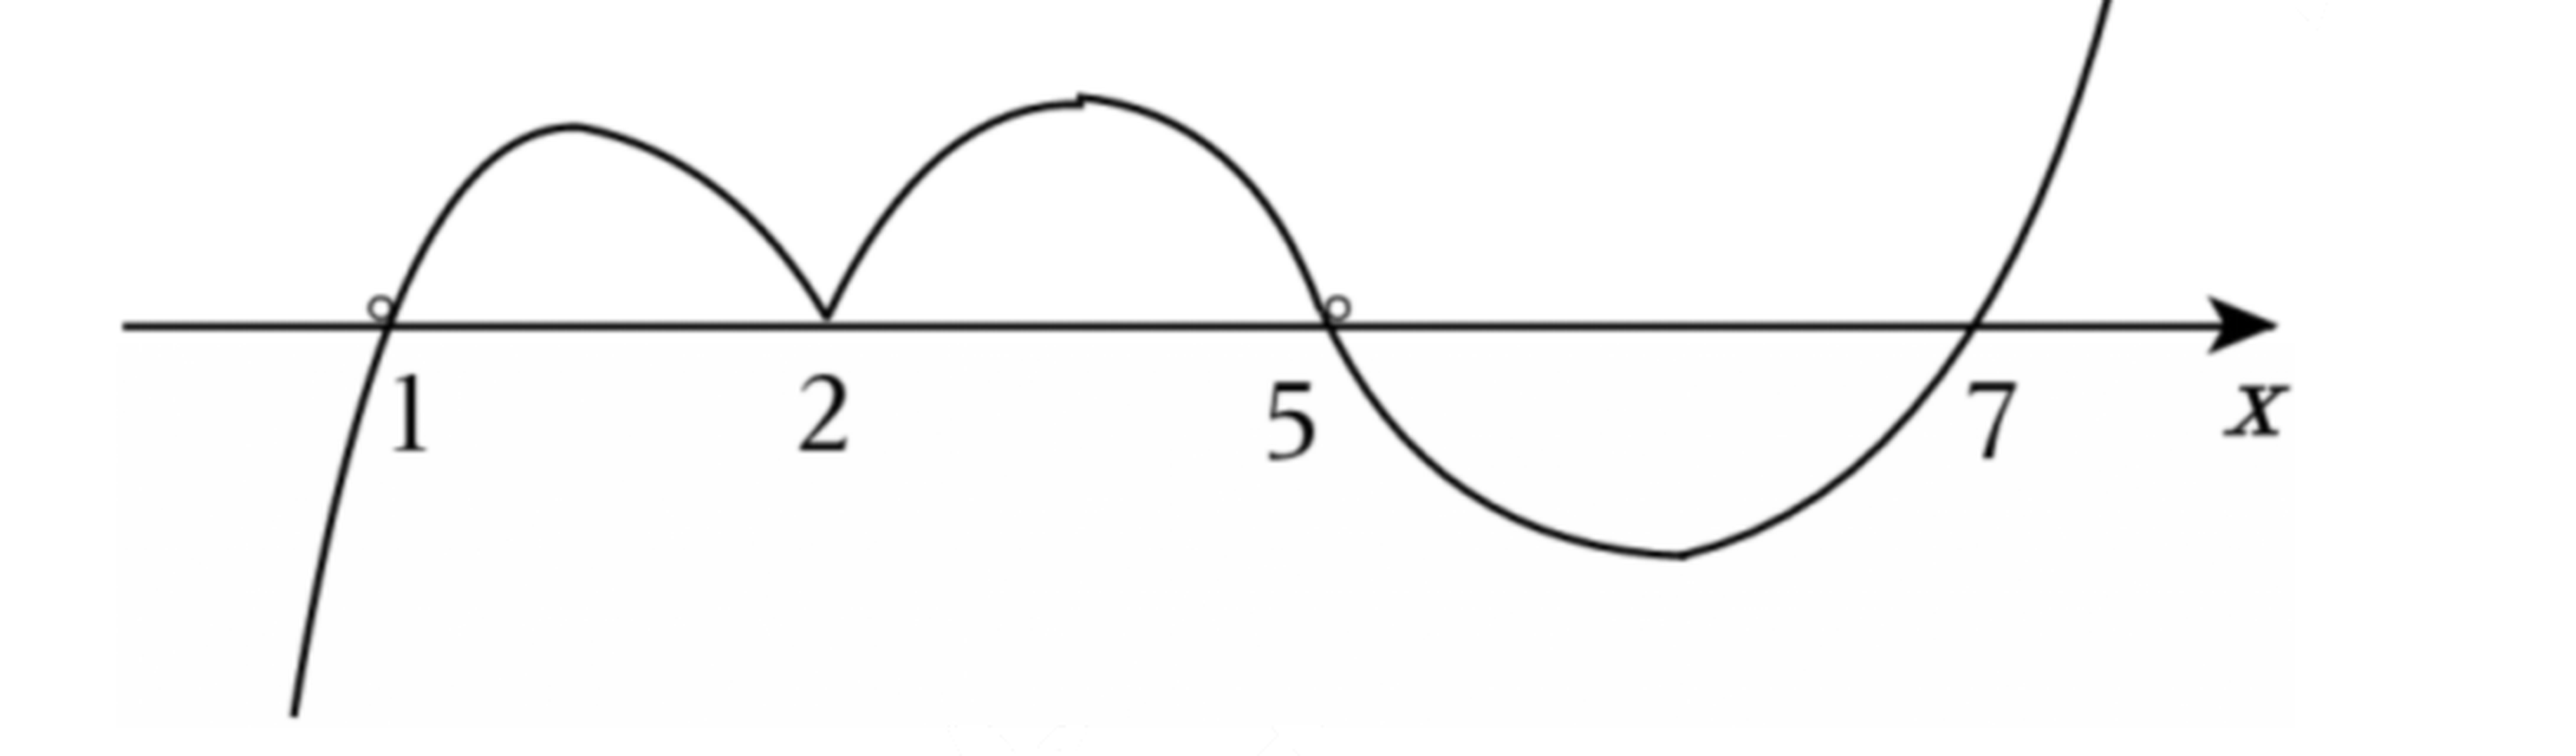
\includegraphics[width=0.62\textwidth]{figures/gao145_q16_a7.png}
\end{center}
\step{得不等式的解集为 $\{x\mid x<1\text{ 或 }x=2\text{ 或 }5<x\leqslant7\}$，}
\step{对应的正整数解为 $2$，$6$，$7$，满足题意，故 $A$ 正确，$C$ 错误.}
\step{故选 $A$.}
\solend
\fi

\end{enumerate}

\bigsec{三、解答题}

\begin{enumerate}
\setcounter{enumi}{16}

% 第 17 题：题干在 06 页、解析续至 07 页，按印刷行断，共 7 行；
% "lg(10÷5)" 的除号照录 \div
\item (1) 已知 $a+a^{-1}=6$，求 $a^2+a^{-2}$ 及 $a^{\frac12}-a^{-\frac12}$ 的值；

(2) 已知 $\lg5=a$，$\lg6=b$，用 $a$、$b$ 分别表示 $\lg2$、$\lg3$、$\lg300$ 和 $\log_{12}15$.

\ifanswer
\solbegin
\step{(1) 因为 $a+a^{-1}=6$，}
\step{所以 $a^2+a^{-2}=(a+a^{-1})^2-2\cdot a\cdot a^{-1}=6^2-2=34$，}
\step{因为 $\left(a^{\frac12}-a^{-\frac12}\right)^2=a-2+a^{-1}=6-2=4$，所以 $a^{\frac12}-a^{-\frac12}=\pm2$；}
\step{(2) $\lg2=\lg(10\div5)=\lg10-\lg5=1-a$，}
\step{$\lg3=\lg(6\div2)=\lg6-\lg2=b-(1-a)=a+b-1$，}
\step{$\lg300=\lg(3\times10^2)=\lg3+\lg10^2=a+b-1+2=a+b+1$，}
\step{所以 $\log_{12}15=\dfrac{\lg15}{\lg12}=\dfrac{\lg3+\lg5}{\lg3+\lg2^2}=\dfrac{a+b-1+a}{a+b-1+2(1-a)}=\dfrac{2a+b-1}{b-a+1}$.}
\solend
\fi

% 第 18 题：题干在 07 页、解析续至 08 页（2 问、分类讨论很长），按印刷行断共 25 行；
% 本卷 Q18 用"图像"（Q13/Q14 用"图象"），逐处照录不统一
\item 已知 $f(x)=(m^2-3m+1)x^{m^2-4m-1}$，$y=f(x)$ 为幂函数且在 $(0,+\infty)$ 上是严格减函数.

(1) 求实数 $m$ 的值以及相应的函数表达式；

(2) 若 $y=f(x)$ 的图像关于 $y$ 轴对称，解关于 $x$ 的不等式 $(x+2)^{1-m}<(3x-1)^{1-m}$.

\ifanswer
\solbegin
\step{(1) 由幂函数的定义得 $m^2-3m+1=1$，}
\step{整理得 $m^2-3m=0$，解得 $m=0$ 或 $m=3$，}
\step{由于 $y=f(x)$ 在 $(0,+\infty)$ 上为严格减函数，}
\step{因此幂函数的指数需满足 $m^2-4m-1<0$，}
\step{当 $m=3$ 时，指数为 $3^2-4\times3-1=-4<0$，满足严格递减条件，}
\step{此时函数表达式为 $f(x)=x^{-4}$，}
\step{当 $m=0$ 时，指数为 $0^2-4\times0-1=-1<0$，满足严格递减条件，}
\step{此时函数表达式为 $f(x)=x^{-1}$，}
\step{所以满足条件的实数 $m$ 为 $0$ 或 $3$，}
\step{对应的函数表达式分别为 $f(x)=x^{-1}$、$f(x)=x^{-4}$；}
\step{(2) 函数图像关于 $y$ 轴对称即函数为偶函数，}
\step{对于 $f(x)=x^{-1}=\dfrac1x$，定义域为 $(-\infty,0)\cup(0,+\infty)$，}
\step{满足 $f(-x)=-f(x)$，为奇函数，图像关于原点对称，}
\step{不满足关于 $y$ 轴对称的条件；}
\step{对于 $f(x)=x^{-4}=\dfrac{1}{x^4}$，定义域为 $(-\infty,0)\cup(0,+\infty)$，}
\step{满足 $f(-x)=f(x)$，为偶函数，图像关于 $y$ 轴对称，}
\step{因此符合条件的 $m$ 值为 $3$，}
\step{将 $m=3$ 代入关于 $x$ 的不等式 $(x+2)^{1-m}<(3x-1)^{1-m}$，}
\step{得 $(x+2)^{1-3}<(3x-1)^{1-3}$，即 $(x+2)^{-2}<(3x-1)^{-2}$，}
\step{因为负指数幂的底数不能为 $0$，所以 $x+2\ne0$ 且 $3x-1\ne0$，}
\step{即 $x\ne-2$ 且 $x\ne\dfrac13$，}
\step{不等式可变形为 $\dfrac{1}{(x+2)^2}<\dfrac{1}{(3x-1)^2}$，}
\step{整理得 $(3x-1)^2<(x+2)^2$，即 $8x^2-10x-3<0$，}
\step{解得 $-\dfrac14<x<\dfrac32$，又 $x\ne-2$ 且 $x\ne\dfrac13$，}
\step{所以不等式的解集为 $\left(-\dfrac14,\dfrac13\right)\cup\left(\dfrac13,\dfrac32\right)$.}
\solend
\fi

% 第 19 题：题干在 08 页、解析续至 09 页，按印刷行断，共 14 行；
% 判别式 cases 块内"△=4a²−16a<0"原卷印扁等边三角 \triangle
%（放大 09 页 zz09_delta.png 与 Q12 高 \Delta 并排确认），逐处照录不统一
\item 已知 $f(x)=ax^2+2ax+4$，$a\in\R$.

(1) 若关于 $x$ 的不等式 $f(x)>0$ 在实数集 $\R$ 上恒成立，求实数 $a$ 的取值范围；

(2) 当 $a<0$ 时，解关于 $x$ 的不等式 $f(x)>(a+1)x+5$.

\ifanswer
\solbegin
\step{(1) 由题意得，关于 $x$ 的不等式 $f(x)>0$ 在实数集 $\R$ 上恒成立，}
\step{即 $ax^2+2ax+4>0$ 在实数集 $\R$ 上恒成立，}
\step{当 $a=0$ 时，不等式为 $4>0$ 恒成立，符合题意；}
\step{当 $a\ne0$ 时，则 $\begin{cases}a>0\\\triangle=4a^2-16a<0\end{cases}$，解得 $0<a<4$.}% 判别式原卷印扁等边三角 $\triangle$，照录
\step{综上所述，实数 $a$ 的取值范围为 $[0,4)$.}
\step{(2) $f(x)=ax^2+2ax+4$，}
\step{当 $a<0$ 时，不等式 $f(x)>(a+1)x+5$ 即为 $ax^2+(a-1)x-1>0$，}
\step{即 $(ax-1)(x+1)>0$，即 $\left(x-\dfrac1a\right)(x+1)<0$，}
\step{当 $a<-1$，即 $\dfrac1a>-1$ 时，解得 $-1<x<\dfrac1a$；}
\step{当 $a=-1$，即 $\dfrac1a=-1$ 时，解得 $x\in\varnothing$；}
\step{当 $-1<a<0$，即 $\dfrac1a<-1$ 时，解得 $\dfrac1a<x<-1$.}
\step{综上所述，当 $a<-1$ 时，不等式的解集为 $\left\{x\mid -1<x<\dfrac1a\right\}$；}
\step{当 $a=-1$ 时，不等式的解集为 $\varnothing$；}
\step{当 $-1<a<0$ 时，不等式的解集为 $\left\{x\mid \dfrac1a<x<-1\right\}$.}
\solend
\fi

% 第 20 题：菜园靠墙图为题目配图（三版都出），题干写"如图"；
% 题干在 09 页（含图）、解析续至 10 页，按印刷行断，共 13 行
\needvspace{8cm}
\item 如图，某人计划用篱笆围成一个一边靠墙（墙足够长）的矩形菜园. 设菜园的长为 $x$ 米，宽为 $y$ 米.

\begin{center}
% 矩形菜园靠墙图取 09 页右下，去粉色水印、去色、4× LANCZOS 放大
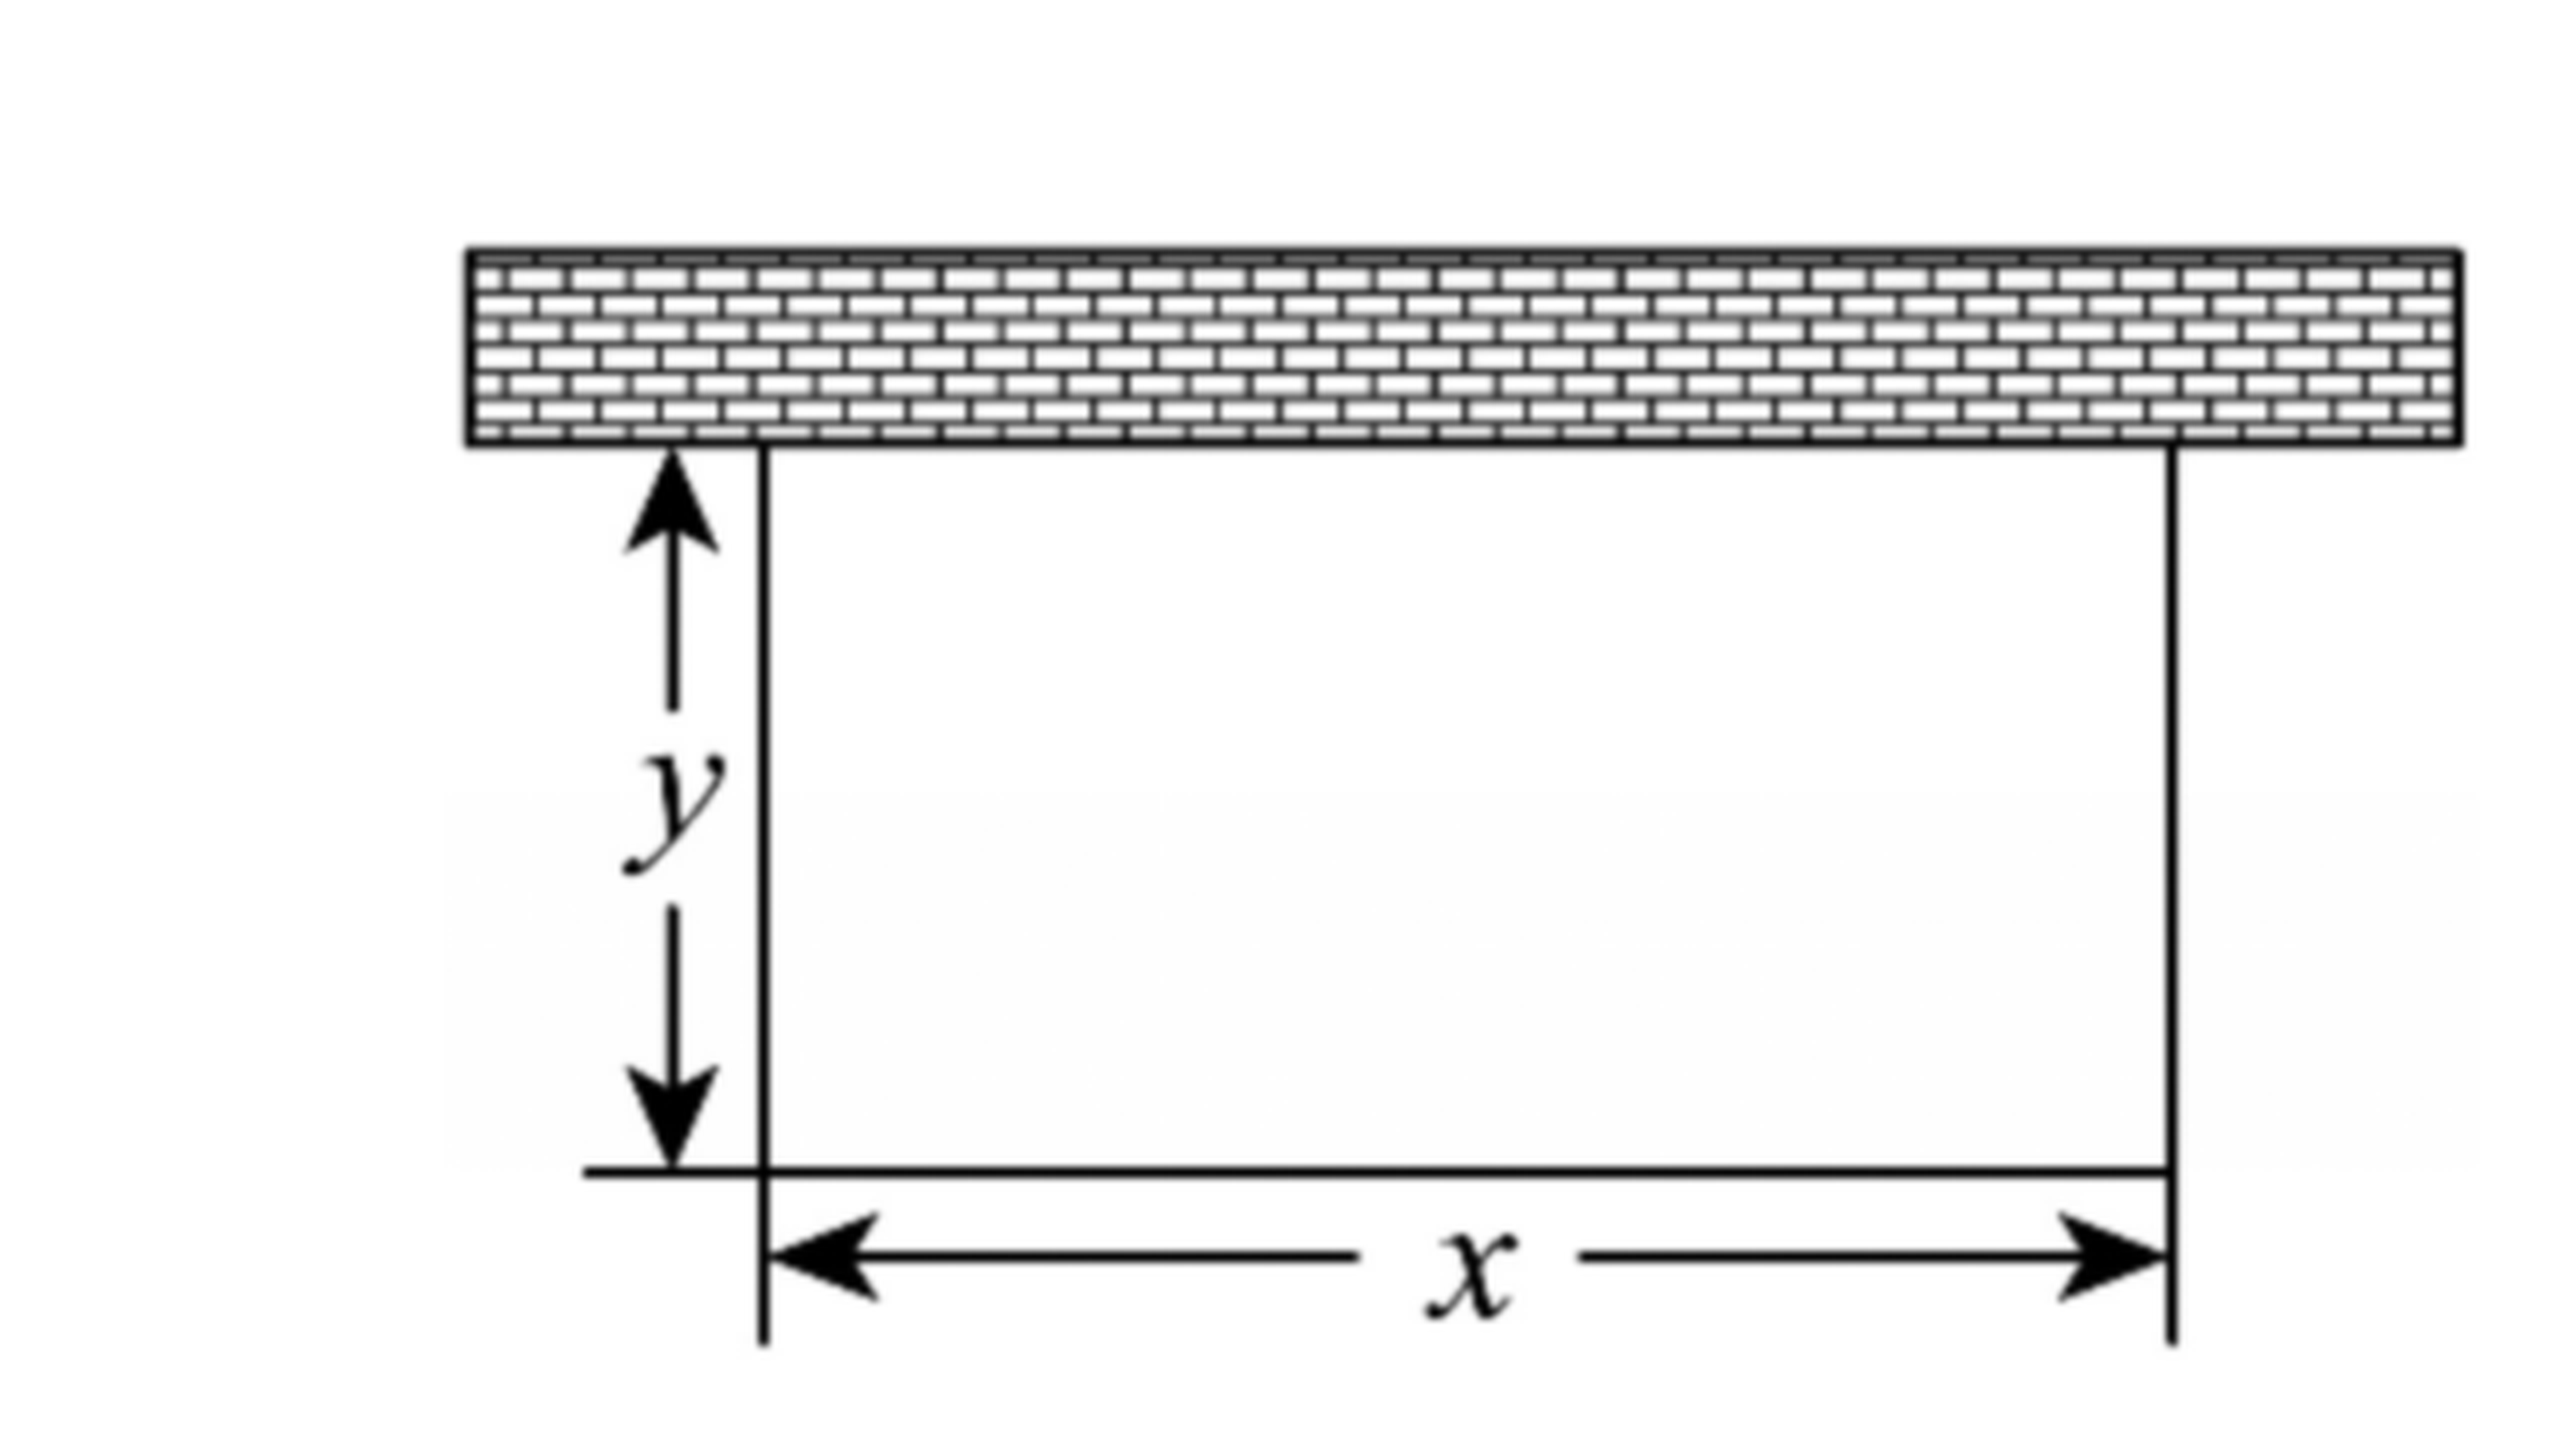
\includegraphics[width=0.55\textwidth]{figures/gao145_q20.png}
\end{center}

(1) 若菜园面积为 72 平方米，则 $x$、$y$ 为何值时，所用篱笆总长最小？

(2) 若 $x$、$y$ 满足 $x+y-xy+63=0$，则菜园面积最小为多少平方米？

\ifanswer
\solbegin
\step{(1) 由题意得，菜园的面积 $S=xy=72$，且 $x>0$，$y>0$，}
\step{所用篱笆总长 $L=x+2y$，}
\step{由基本不等式得 $x+2y\geqslant2\sqrt{x\cdot2y}=2\sqrt{2xy}=2\sqrt{2\times72}=24$，}
\step{当且仅当 $x=2y$ 时取等号，}
\step{联立 $\begin{cases}xy=72\\x=2y\end{cases}$，解得 $\begin{cases}x=12\\y=6\end{cases}$，}
\step{所以当 $x=12$，$y=6$ 时，所用篱笆总长最小；}
\step{(2) 由题意得 $x>0$，$y>0$，且满足 $x+y-xy+63=0$，即 $x+y=xy-63$，}
\step{由基本不等式得 $x+y\geqslant2\sqrt{xy}$，当且仅当 $x=y$ 时取等号，}
\step{所以 $xy-63\geqslant2\sqrt{xy}$. 令 $t=\sqrt{xy}(t>0)$，则 $xy=t^2$，}
\step{上述不等式可化为 $t^2-2t-63\geqslant0$，即 $(t-9)(t+7)\geqslant0$，}
\step{因为 $t>0$，所以 $t+7>0$，故 $t-9\geqslant0$，解得 $t\geqslant9$，所以 $\sqrt{xy}\geqslant9$，}
\step{即 $xy\geqslant81$，当且仅当 $x=y=9$ 时取等号，此时满足 $9+9-81+63=0$，}
\step{所以菜园面积最小为 81 平方米.}
\solend
\fi

% 第 21 题：题干在 10 页、解析续至 11 页（3 问、分类讨论很长），按印刷行断共 22 行；
% 末行"故第 2026 个元素是 2700 之后第一个属于 A 的数，即 2701." 为全卷收尾，
% 无 Q22/Q23、无附加题节；数集 Z/N* 按全稿惯例改 \Z/\N^*
\item 已知集合 $A=\{x\mid x=m^2-n^2$，$m$、$n\in\Z\}$.

(1) 求证：任何奇数 $2k+1(k\in\Z)$ 都是集合 $A$ 中的元素；

(2) 判断偶数 $4k-2(k\in\Z)$ 是否为集合 $A$ 的元素？请说明理由；

(3) 若将集合 $A$ 中的正整数由小到大排列，求出集合 $A$ 中第 2026 个正整数.

\ifanswer
\solbegin
\step{(1) 因为 $x=(k+1)^2-k^2=2k+1(k\in\Z)$，}
\step{所以任何奇数 $2k+1(k\in\Z)$ 都属于集合 $A$；}
\step{(2) 偶数 $4k-2(k\in\Z)$ 不是集合 $A$ 的元素，理由如下：}
\step{由题意得 $x=m^2-n^2=(m-n)(m+n)$，}
\step{当 $m$、$n$ 均为奇数时，设 $m=2k_1+1$，$n=2k_2+1(k_1$、$k_2\in\Z)$，}
\step{则 $m^2-n^2=(2k_1+1)^2-(2k_2+1)^2=(2k_1-2k_2)(2k_1+2k_2+2)$}
\step{$=4(k_1-k_2)(k_1+k_2+1)$，}
\step{因为 $k_1$、$k_2\in\Z$，所以 $k_1-k_2\in\Z$，$k_1+k_2+1\in\Z$，}
\step{从而 $m^2-n^2$ 为 $4$ 的倍数；}
\step{当 $m$、$n$ 均为偶数时，设 $m=2k_1$，$n=2k_2(k_1$、$k_2\in\Z)$，}
\step{$m^2-n^2=4k_1^2-4k_2^2=4(k_1^2-k_2^2)$ 为 $4$ 的倍数；}
\step{当 $m$、$n$ 为一个偶数一个奇数时，不妨设 $m$ 为偶数，$n$ 为奇数，}
\step{设 $m=2k_1$，$n=2k_2+1(k_1$、$k_2\in\Z)$，}
\step{则 $m^2-n^2=4k_1^2-(2k_2+1)^2=4(k_1^2-k_2^2-k_2)-1$ 为奇数.}
\step{无论哪种情况均不满足 $4k-2(k\in\Z)$，}
\step{故偶数 $4k-2(k\in\Z)$ 不是集合 $A$ 的元素；}
\step{(3) 由前两问得，$4$ 的倍数和奇数属于集合 $A$ 中的元素，}
\step{令集合 $A$ 中的正整数元素为 $4k-3$、$4k-1$、$4k(k\in\N^*)$，}
\step{对任意的 $k\in\N^*$，连续的 $4$ 个整数 $4k-3$、$4k-2$、$4k-1$、$4k$ 中}
\step{有三个数 $4k-3$、$4k-1$、$4k$ 都在集合 $A$ 中，}
\step{因为 $2026=3\times675+1$，所以集合 $A$ 中第 $2025$ 个元素为 $4\times675=2700$，}
\step{故第 2026 个元素是 2700 之后第一个属于 $A$ 的数，即 2701.}
\solend
\fi

\end{enumerate}

\end{document}
"
%
% ① 原始材料：微信公众号"魔都数学加油站"文章，连载"27学年高一145"，原文标题
% "27学年高一145——2026-2027年上海市市二中学高一上期中"；
% 原文链接：https://mp.weixin.qq.com/s/6V-i9KE0GWodC-wmd5z8nQ 。
% 正文为 11 张 PNG 页（01/02/03/08/10/11 为 4762×6735，04/05/06/07/09 为 2560×3620，
% 同一篇各页分辨率不同，逐页按各自分辨率裁图核对，别按预览比例换算裁框）。
% 题目下印【答案】或【解析】，为混合体例讲评版：Q3 只印【答案】、无【解析】，其余
% 18 题印【解析】。题目、解析均据原图转录；卷面粉红色水印"魔都数学加油站"及
% 公众号页脚未录入。
% 全卷插图情况（逐页通读 11 页确认，题干写"如图"处均配有图）：
%   · Q14 韦恩图（05 页右侧，全集 U 矩形＋两圆 M/N＋白色交集、灰色阴影＋U/M/N 标注）：
%     题目配图（选择题选项旁），三版都出，裁自 05 页去水印去色 4× 放大存
%     figures/gao145_q14.png；
%   · Q16 两幅数轴标根波浪曲线（06 页，a=3 与 a=7 各一幅，标根法画
%     (x-1)(x-2)^2(x-5)(x-a)≤0 的符号曲线）：【解析】内的配图，仅答案版出，
%     裁 figures/gao145_q16_a3.png / figures/gao145_q16_a7.png（或合并一张），
%     放在答案版条件块内 \solbegin 的 \step 之间（照 高一73 第 16 题成例）；
%   · Q20 矩形菜园靠墙图（09 页右下，灰色砖墙＋矩形菜园＋x/y 标注＋箭头）：
%     题目配图，三版都出，裁自 09 页去水印去色 4× 放大存 figures/gao145_q20.png；
%   其余各页逐页确认无其它题目配图、无表格、亦无"题干写如图而源码漏图"一处。
%
% 卷首标题：原卷印作"2026-2027 年市二中学高一上期中"，年份区间按全稿惯例排 en dash；
% 原卷卷面未印副标题，本稿按同期中卷（高一140／141／143／144）知识模块口径补出
% "集合与常用逻辑用语、不等式、函数"。
%
% 题号体例：本卷共 19 题——一、填空题 3—12（10 题）、二、选择题 13—16（4 题）、
% 三、解答题 17—21（5 题）。三节分别 \setcounter{enumi}{2}／{12}／{16}。
% 原卷从第 3 题起、无第 1、2 题，本稿保留原题号；全卷无附加题节。
%
% ② 与原卷的排版差异：
%   ① 原文从第 3 题起，本稿保留原题号；共 19 题三节；
%   ② 混合体例：原卷 Q3 只印【答案】、无【解析】（"第一步应假设___。
%      【答案】x≤2 或 y≤2"），按 高一140 第 5 题成例提 \ans{}、不补造解析；
%      其余 18 题印【解析】，用 \solbegin…\solend，选择题答案在解析末句"故选 X"
%      （Q13 选 B、Q14 选 D、Q15 选 D、Q16 选 A，逐个放大原图核实）、
%      题干括号 \mbox{（\quad）} 留空、不另提 \ans{}；填空／解答答案落在解析里；
%      答案版【答案】/【解析】标记数 = 19（1 个 \ans ＋ 18 个 \solbegin）= 全卷题数；
%   ③ 原卷卷面未印副标题，本稿按知识模块口径补出；
%   ④ 原卷填空横线按全稿惯例排 \blankline[4.4em]；选择题括号排 \mbox{（\quad）}、
%      选项段前按惯例加 \keepwithprev；解答题不留作答区、不加 \anspace
%      （原卷为讲评版，与 129／131／132／133／136／140／141／143／144 同）；
%   ⑤ 数集：Q9"a、b∈R"、Q12"a∈R"、Q21"m、n∈Z""k∈Z""k∈N*"等原卷印
%      斜体或黑板粗体 R/Z/N，按全稿惯例统一改 \R／\Z／\N^*；绝对值排 \lvert…\rvert，
%      集合描述竖线排 \mid；不等号按全稿惯例排 \leqslant／\geqslant；
%      补集照原卷上划线排 \overline{M}／\overline{N}（Q14 选项 B/C/D 逐处核）；
%      空集记号 \varnothing；\subset（单线⊂）与 \subseteq（带下划线⊆）逐处照录不统一；
%   ⑥ 子题标号 (1)(2)(3) 原卷印半角括号照录；圈数字进数学式用 \text{①}（否则 FONTCHK 挂）；
%      \left…\right 不得拆到不同 $…$ 组；cases 块整体算一个印刷行；
%   ⑦ 题干／解析中的中文弯引号按原卷照录（Q3"若 x+y>4，则 x>2 且 y>2"、
%      Q11"a₁/a₂=b₁/b₂""M=N"、选填"充分非必要""必要非充分""充要""既非充分也非必要"
%      等，含引号内空格），注释内一律 ASCII 引号；数学式内 CJK 用 \text{}；
%   ⑧ 半角逗号在数学组之间是全稿惯例、非笔误（如 Q5"x₁+x₂=6，x₁x₂=√3"、
%      Q7"a>1，b>1"、指数／对数式内逗号），逐处照录别改全角；行末西文句点照录为
%      ASCII `.`；行中全角逗号／顿号照录；
%   ⑨ "图像／图象"逐处照录不统一（Q18"图像关于 y 轴对称"等，核全卷）；
%   ⑩ 判别式 Δ/△ 混用是照录项：Q12 解析"Δ=a²−4a²(2a−3)>0"、
%      Q19 解析"Δ=4a²−16a<0"等，放大原图判断是高 \Delta（等腰偏高、高>宽）
%      还是扁 \triangle，逐处照录不得统一（参照 高一142／144 头注④口径）；
%   ⑪ 一条 \step = 原卷解析的一个印刷行，cases 块整体算一个印刷行；别把原卷折行
%      并起来、别把一行拆多条。Q6 分段讨论、Q12 三个 cases 条件组、Q16 数轴标根、
%      Q18／Q19 分类讨论、Q21 三问均按印刷行逐条断，不丢行；
%   ⑫ Q14 韦恩图为"题干＋选项＋图"整块，加 \needvspace 守卫推走（守卫放 \item 之前，
%      见 高一140 Q14、高一144 Q17 成例与切页审计 B 类坑）；Q20 菜园图同理；
%      三版切页审计均"合计异常：无"；
%   ⑬ 跨页续印按题合并：Q3/4/5/6 在 01 页（Q6 解析续 02 页顶）；Q7/8/9/10 在 02 页
%      （Q10 解析续 03 页）；Q11/12 在 03 页（Q12 解析续 04 页，很长）；
%      Q13 在 04 页末、解析在 05 页顶；Q14/15/16 在 05 页（Q16 解析续 06 页含两幅数轴图）；
%      Q17 在 06 页、解析续 07 页；Q18 在 07 页、解析续 08 页；Q19 在 08 页、解析续 09 页；
%      Q20 在 09 页（含菜园图）、解析续 10 页；Q21 在 10 页、解析续 11 页
%      （末页收尾"故第 2026 个元素是 2700 之后第一个属于 A 的数，即 2701."、
%      无 Q22/Q23、无附加题节）。本稿按题连排，不丢行、不并折行；
%   ⑭ 原卷解析内若有红色"法一／法二"之类小标题，按全稿惯例排 \stepm{标签}{…}
%      （黑体着色、不引入红色、不改 common.sty），头注注明；水印"魔都数学加油站"
%      红色不录入。
%
% ③ 行数复核：一条 \step／\stepm = 原卷解析的一个印刷行，cases 块作一个印刷行计。
%   逐题数（主会话逐页核对定稿）：Q3：0（只印【答案】、提 \ans{}，不计入 \step 账）；
%   Q4：3；Q5：2；Q6：10；Q7：3；Q8：3；Q9：2；Q10：7；Q11：4；Q12：12；
%   Q13：2；Q14：2；Q15：4；Q16：9；Q17：7；Q18：25；Q19：14；Q20：13；Q21：22。
%   合计 144 条 \step（本卷无 \stepm：解析内无红色"法一／法二"类小标题），
%   与原卷逐题印刷行相等。全卷 18 题设 \solbegin…\solend ＋ Q3 一处 \ans{}，
%   答案版【答案】/【解析】标记数 = 19 = 全卷题数。
%
% ④ 判别式／子集符号结论（逐处放大原图照录、不得统一，主会话像素级复核）：
%   判别式全卷 2 处、两形混用逐处照录不统一（参照 高一142／144 头注④口径）：
%     · Q12 解析 cases 块"Δ=a²−4a²(2a−3)>0" 原卷印等腰偏高粗三角（高>宽），
%       照录 \Delta（放大 04 页 /tmp/gao145s2/main_q12_delta.png 确认）；
%     · Q19 解析 cases 块"△=4a²−16a<0" 原卷印扁等边空心三角（宽≈高、细线），
%       照录 \triangle（放大 09 页 /tmp/gao145s2/main_q19_delta.png 确认）。
%   子集／补集：Q14 选项 A `M\cup N`、B `M\cap\overline{N}`（上划线只在 N 上）、
%   C `\overline{M\cup N}`（罩整个 M∪N）、D `\overline{M\cap N}`（罩整个 M∩N，
%   非 \overline{M}\cap N；放大 05 页 /tmp/gao145s2/main_q14_opts.png 确认），
%   阴影为灰色区域＝全集减白色交集，答案 D，照录 \overline{M\cap N}；
%   全集卷无 \subset／\subseteq 混用（本卷集合题用 \cup／\cap／\overline{}）；
%   空集 \varnothing（Q19 解析 x∈\varnothing）；数集 \R／\Z／\N^* 归一见 ② ⑤。
%
% ⑤ 存疑照录（放大原图确认，照录未改、正文对应处另有 % 注）：
%   1. Q3 题干"若 x+y>4，则 x>2 且 y>2" 后"时"前留一空格、弯引号内空格照录；
%      该卷混合体例（Q3 只印【答案】、提 \ans{}）见 ② ②。
%   2. Q4／Q5 解析中的"1，3，5 和 6"、"x₁+x₂=6,x₁x₂=√3" 等半角／全角逗号
%      逐处照原卷（放大 01 页确认），数学式内半角逗号为全稿惯例、非笔误。
%   3. Q14 选项 D 上划线罩住整个 M∩N（而非仅罩 M），照录 \overline{M\cap N}。
%   4. Q12 判别式高 \Delta 与 Q19 判别式扁 \triangle 两形混用，逐处照录不统一（见 ④）。
%   全卷除此 4 类外未发现其它笔误／自相矛盾处。
%
% ⑥ 跨页续印按题合并说明：见 ② ⑬。
%
\documentclass[a4paper,11pt]{article}
\usepackage{common}

\begin{document}

\examtitlest[3]{2026--2027 年市二中学高一上期中}{集合与常用逻辑用语、不等式、函数}

\bigsec{一、填空题}

\begin{enumerate}
\setcounter{enumi}{2}

% 第 3 题：原卷只印【答案】、无【解析】（放大 01 页确认），按 高一140 第 5 题成例
% 提 \ans{}、不补造解析；题干中文弯引号与"时"前空格照录
\item 用反证法证明命题：“若 $x+y>4$，则 $x>2$ 且 $y>2$” 时，第一步应假设\blankline[4.4em].

\ifanswer
\ans{$x\leqslant2$ 或 $y\leqslant2$}
\fi

% === Q4 ===
\item 设集合 $M$ 满足 $\{1,3,5,6\}\cup M=\{1,2,3,4,5,6\}$，则满足条件的所有 $M$ 的个数为\blankline[4.4em].

\ifanswer
\solbegin
\step{集合 $M$ 满足 $\{1,3,5,6\}\cup M=\{1,2,3,4,5,6\}$，}
\step{则 $M$ 中必含有 $2$ 和 $4$，$1$，$3$，$5$ 和 $6$ 可以选也可不选，}
\step{则满足条件的所有 $M$ 的数目相当于集合 $\{1,3,5,6\}$ 的子集的个数 $2^4=16$.}
\solend
\fi

% === Q5 ===
\item 已知方程 $x^2-6x+\sqrt3=0$ 的两根为 $x_1$ 和 $x_2$，则 $(x_1-x_2)^2=$\blankline[4.4em].

\ifanswer
\solbegin
\step{因为方程 $x^2-6x+\sqrt3=0$ 的两根为 $x_1$ 和 $x_2$，所以 $x_1+x_2=6,x_1x_2=\sqrt3$，}% 数学式内半角逗号为全稿惯例，照录
\step{所以 $(x_1-x_2)^2=(x_1+x_2)^2-4x_1x_2=36-4\sqrt3$.}
\solend
\fi

% 第 6 题：题干在 01 页，解析续至 02 页顶（末 2 行），按印刷行逐条断，共 10 行
\item 不等式 $\lvert x-2026\rvert+\lvert x-2029\rvert>3$ 的解集是\blankline[4.4em].

\ifanswer
\solbegin
\step{当 $x<2026$ 时，$x-2026<0$，$x-2029<0$，}
\step{原不等式可化为 $(2026-x)+(2029-x)>3$，解得 $x<2026$，}
\step{故此时，不等式的解为 $x<2026$；}
\step{当 $2026\leqslant x\leqslant2029$ 时，$x-2026\geqslant0$，$x-2029\leqslant0$，}
\step{原不等式可化为 $(x-2026)+(2029-x)>3$，即 $3>3$，显然不成立，}
\step{故此时，不等式无解；}
\step{当 $x>2029$ 时，$x-2026>0$，$x-2029>0$，}
\step{原不等式可化为 $(x-2026)+(x-2029)>3$，解得 $x>2029$，}
\step{故此时，不等式的解为 $x>2029$.}
\step{综上，原不等式的解集为 $(-\infty,2026)\cup(2029,+\infty)$.}
\solend
\fi

% === Q7 ===
\item 已知 $a>1$，$b>1$，若 $\log_a b+\log_b a=2$，且 $ab=2$，则 $\log_2(a+b)=$\blankline[4.4em].

\ifanswer
\solbegin
\step{由 $\log_a b+\log_b a=2$，$a>1$，$b>1$，得 $\log_a b+\dfrac{1}{\log_a b}=2$，}
\step{即 $(\log_a b)^2-2\log_a b+1=0$，则 $(\log_a b-1)^2=0$，解得 $\log_a b=1$，即 $a=b$，}
\step{又 $ab=2$，所以 $a=b=\sqrt2$，所以 $\log_2(a+b)=\log_2 2\sqrt2=\log_2 2^{\frac32}=\dfrac32$.}
\solend
\fi

% === Q8 ===
\item 已知 $m>0$，$n>0$，且 $m+n=1$，则 $\dfrac1m+\dfrac4n$ 的最小值为\blankline[4.4em].

\ifanswer
\solbegin
\step{由 $m>0$，$n>0$，$m+n=1$，}
\step{则 $\dfrac1m+\dfrac4n=(m+n)\left(\dfrac1m+\dfrac4n\right)=5+\dfrac nm+\dfrac{4m}n\geqslant5+2\sqrt{\dfrac nm\cdot\dfrac{4m}n}=9$，}
\step{当且仅当 $n=2m=\dfrac23$ 时，上式取得等号，故最小值为 $9$.}
\solend
\fi

% === Q9 ===
\item 已知 $a$、$b\in\R$，且 $3a+2b=1$，则 $8^a+4^b$ 最小值为\blankline[4.4em].

\ifanswer
\solbegin
\step{因为 $3a+2b=1$，所以 $8^a+4^b=2^{3a}+2^{2b}\geqslant2\sqrt{2^{3a+2b}}=2\sqrt2$，}
\step{当且仅当 $3a=2b$ 时取等号，故最小值为 $2\sqrt2$.}
\solend
\fi

% 第 10 题：题干在 02 页、解析续至 03 页顶，按印刷行断，共 7 行
\item 已知关于 $x$ 的不等式 $ax^2+bx+c>0$ 的解集为 $\{x\mid 1<x<2\}$，则关于 $x$ 的不等式 $bx^2-ax+c<0$ 的解集为\blankline[4.4em].

\ifanswer
\solbegin
\step{已知关于 $x$ 的不等式 $ax^2+bx+c>0$ 的解集为 $\{x\mid 1<x<2\}$，}
\step{由解集为 $1<x<2$ 且二次函数在两根之间为正，得 $a<0$，两个根为 $1$，$2$，}
\step{所以 $ax^2+bx+c=a(x-1)(x-2)=ax^2-3ax+2a$，}
\step{比较系数得 $b=-3a$，$c=2a$.}
\step{于是 $bx^2-ax+c=-3ax^2-ax+2a=-a(3x-2)(x+1)$，}
\step{$a<0$，故 $bx^2-ax+c<0$ 等价于 $(3x-2)(x+1)<0$，解得 $-1<x<\dfrac23$，}
\step{故 $bx^2-ax+c<0$ 的解集为 $\left\{x\mid -1<x<\dfrac23\right\}$.}
\solend
\fi

% 第 11 题：题干引号内空格照录（放大 03 页确认），四组选填引号亦同；
% 结论"故为必要非充分条件"照录，解析共 4 个印刷行
\item 设 $a_1$、$b_1$、$a_2$、$b_2$ 均为非零实数，不等式 $a_1x+b_1>0$ 和 $a_2x+b_2>0$ 的解集分别为集合 $M$、$N$，那么 “ $\dfrac{a_1}{a_2}=\dfrac{b_1}{b_2}$ ” 是 “ $M=N$ ” 的\blankline[4.4em]条件（选填 “ 充分非必要 ”、“ 必要非充分 ”、“ 充要 ” 和 “ 既非充分也非必要 ”）.

\ifanswer
\solbegin
\step{当 $a_1=b_1=1$，$a_2=b_2=-1$ 时，满足 $\dfrac{a_1}{a_2}=\dfrac{b_1}{b_2}$，}
\step{但是 $M=N$ 不成立，即充分性不成立；}
\step{若 $M=N$ 时，$\dfrac{a_1}{a_2}=\dfrac{b_1}{b_2}$ 一定成立，即必要性成立.}
\step{故为必要非充分条件.}
\solend
\fi

% 第 12 题：题干在 03 页、解析续至 04 页（很长，含 3 个 cases 条件组），
% 按印刷行逐条断共 12 行；cases 块整体算一个印刷行
\item 已知 $f(x)=\dfrac{ax+3}{x-2}$（常数 $a\in\R$）. 函数 $y=f(x)$ 在区间 $[3,+\infty)$ 上是严格减函数，且函数值不恒为负. 若关于 $x$ 的方程 $f(x)=\dfrac{a}{ax-1}$ 有两个不相等的实数根 $x_1$ 和 $x_2$，则 $a$ 的取值范围是\blankline[4.4em].

\ifanswer
\solbegin
\step{$f(x)=\dfrac{ax+3}{x-2}=a+\dfrac{3+2a}{x-2}$，定义域 $(-\infty,2)\cup(2,+\infty)$，}
\step{由于 $y=f(x)$ 在区间 $[3,+\infty)$ 上是严格减函数，且函数值不恒为负，}
\step{所以 $\begin{cases}3+2a>0\\a+\dfrac{3+2a}{3-2}\geqslant0\end{cases}\Rightarrow a\geqslant-1$，}
\step{若关于 $x$ 的方程 $f(x)=\dfrac{a}{ax-1}$ 有两个不相等的实数根 $x_1$ 和 $x_2$，}
\step{则 $\dfrac{ax+3}{x-2}=\dfrac{a}{ax-1}$，即 $(ax+3)(ax-1)=a(x-2)$，$x\ne2$ 且 $ax-1\ne0$，}
\step{当 $a\ne0$ 且 $a\geqslant-1$ 时，$(ax+3)(ax-1)=a(x-2)$，$x\ne2$ 且 $ax-1\ne0$，}
\step{可化为 $\begin{cases}a^2x^2+ax+2a-3=0\\x\ne2,x\ne\dfrac1a\end{cases}$，}
\step{要使方程有两个不相等的实数根 $x_1$ 和 $x_2$，}
\step{则 $\begin{cases}\Delta=a^2-4a^2(2a-3)>0\\a\geqslant-1\text{且}a\ne0\\4a^2+2a+2a-3\ne0\\a^2\cdot\dfrac1{a^2}+a\cdot\dfrac1a+2a-3\ne0\end{cases}\Rightarrow\begin{cases}a<\dfrac{13}{8}\\a\geqslant-1\text{且}a\ne0\\a\ne\dfrac12\text{且}a\ne-\dfrac32\\a\ne\dfrac12\end{cases}$，}% 判别式原卷印等腰偏高三角 $\Delta$，照录（放大 04 页 zz04_delta.png 确认）
\step{得 $-1\leqslant a<\dfrac{13}{8}$ 且 $a\ne0,a\ne\dfrac12$；}
\step{当 $a=0$ 时，方程无解；}
\step{所以 $a$ 的取值范围是 $[-1,0)\cup\left(0,\dfrac12\right)\cup\left(\dfrac12,\dfrac{13}{8}\right)$.}
\solend
\fi

\end{enumerate}

\bigsec{二、选择题}

\begin{enumerate}
\setcounter{enumi}{12}

% 第 13 题：题干在 04 页末、解析在 05 页顶；"图象"照录（本卷 Q13、Q14 用"图象"）
\item 已知幂函数 $f(x)$ 的图象过点 $\left(7,\dfrac{1}{\sqrt7}\right)$，则 $f(x)=$\mbox{（\quad）}

\keepwithprev
A. $x^{-2}$\qquad B. $x^{-\frac12}$\qquad C. $x^{\frac12}$\qquad D. $x^2$

\ifanswer
\solbegin
\step{设幂函数 $f(x)=x^\alpha(\alpha\in\R)$，因为幂函数的图象过点 $\left(7,\dfrac{1}{\sqrt7}\right)$，}
\step{所以 $7^\alpha=\dfrac{1}{\sqrt7}=7^{-\frac12}$，所以 $\alpha=-\dfrac12$，故 $f(x)=x^{-\frac12}$. 故选 $B$.}
\solend
\fi

% 第 14 题：韦恩图为题目配图（三版都出），"题干＋选项＋图"整块，needvspace
% 守卫放在 \item 之前（Q14 为选择题节内第二题，不会让节标题孤落页末）；
% D 选项上划线罩住整个 M∩N（放大 05 页 zz05_q14D.png 确认，非 \overline{M}\cap N）
\needvspace{9cm}
\item 已知全集 $U$ 和集合 $M$、$N$，用集合语言表示图中的阴影部分，正确的是\mbox{（\quad）}

\keepwithprev
A. $M\cup N$\qquad B. $M\cap\overline{N}$\qquad C. $\overline{M\cup N}$\qquad D. $\overline{M\cap N}$

\begin{center}
% 韦恩图取 05 页右侧，去粉色水印、去色、4× LANCZOS 放大
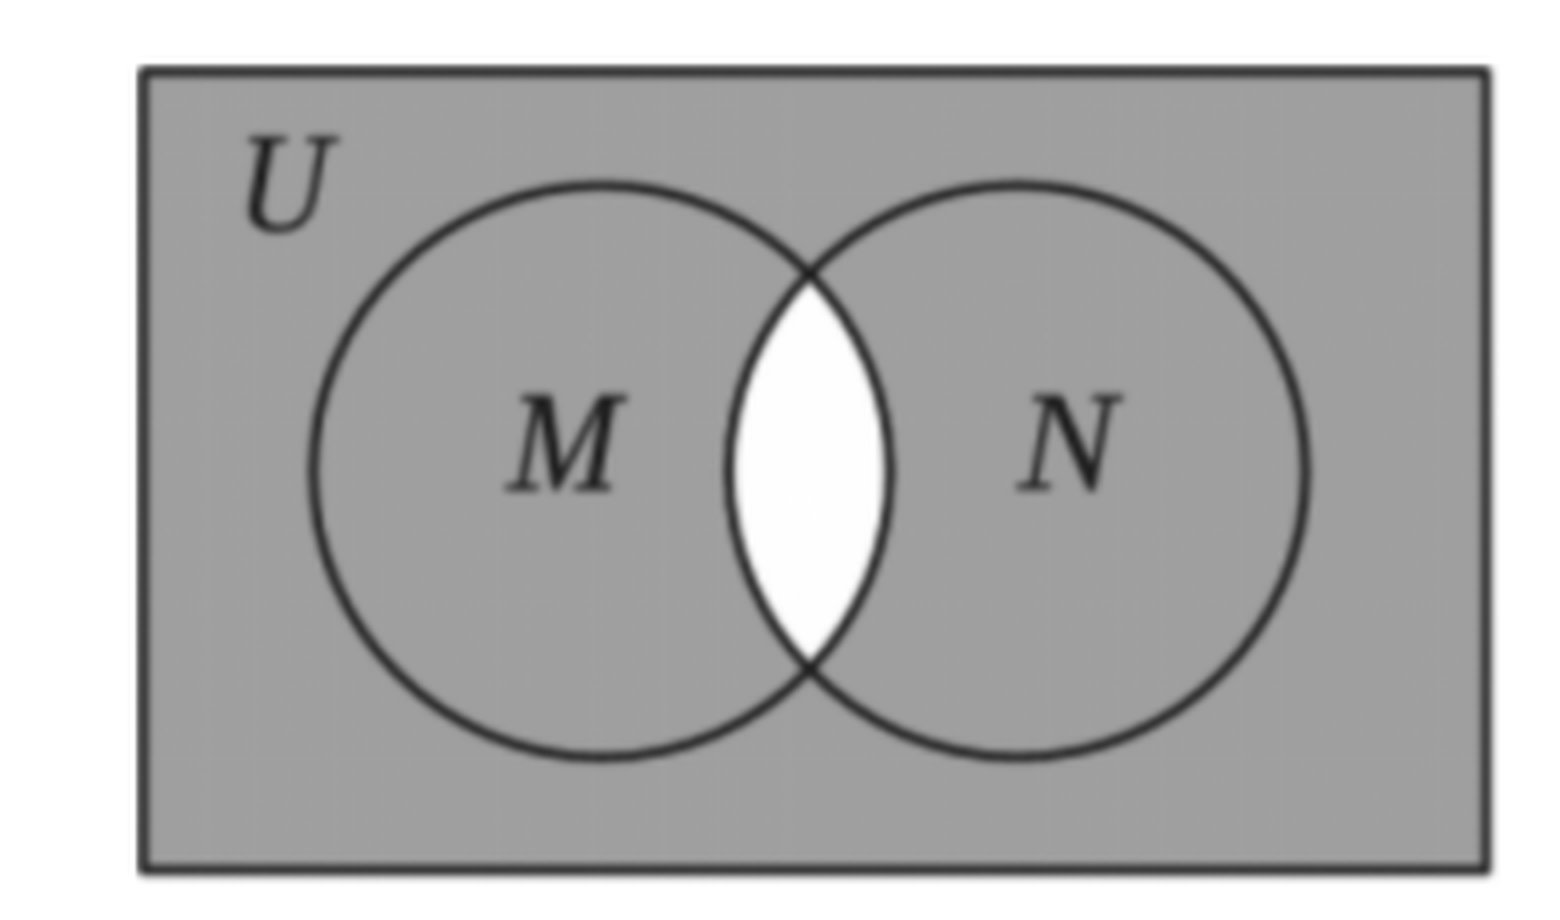
\includegraphics[width=0.40\textwidth]{figures/gao145_q14.png}
\end{center}

\ifanswer
\solbegin
\step{由韦恩图得图中白色区域为集合 $M\cap N$，所以阴影部分表示的集合为 $\overline{M\cap N}$.}
\step{故选 $D$.}
\solend
\fi

% === Q15 ===
\item 已知 $x>-2$，则 $x+\dfrac{1}{x+2}$ 的最小值为\mbox{（\quad）}

\keepwithprev
A. 3\qquad B. 2\qquad C. 1\qquad D. 0

\ifanswer
\solbegin
\step{$x>-2$，则 $x+2>0$，}
\step{所以 $x+\dfrac{1}{x+2}=(x+2)+\dfrac{1}{x+2}-2\geqslant2\sqrt{(x+2)\cdot\dfrac{1}{x+2}}-2=0$，}
\step{当且仅当 $x+2=\dfrac{1}{x+2}$，即 $x=-1$ 时取等号，所以 $x+\dfrac{1}{x+2}$ 的最小值为 $0$.}
\step{故选 $D$.}
\solend
\fi

% 第 16 题：题干在 05 页、解析续至 06 页；两幅数轴标根波浪曲线是【解析】内配图，
% 仅答案版出，放在答案版条件块内 \solbegin 的 \step 之间（照 高一73 第 16 题成例）
\item 关于 $x$ 的不等式 $\dfrac{(x-a)(x-2)^2}{(x-1)(x-5)}\leqslant0$ 的解集中恰有 3 个正整数，则实数 $a$ 的取值范围是\mbox{（\quad）}

\keepwithprev
A. $(-\infty,3]\cup[7,8)$\qquad B. $(-\infty,3)\cup[7,8)$\qquad C. $(-\infty,3]\cup(7,8]$\qquad D. $(-\infty,3)\cup(7,8]$

\ifanswer
\solbegin
\step{由题意，不等式 $\dfrac{(x-a)(x-2)^2}{(x-1)(x-5)}\leqslant0$，}
\step{可化为 $\begin{cases}(x-1)(x-2)^2(x-5)(x-a)\leqslant0\\x\ne1\text{且}x\ne5\end{cases}$，由数轴标根法，}
\step{当 $a=3$ 时，}
\begin{center}
% a=3 数轴标根图取 06 页，去粉色水印、去色、4× LANCZOS 放大；仅答案版出
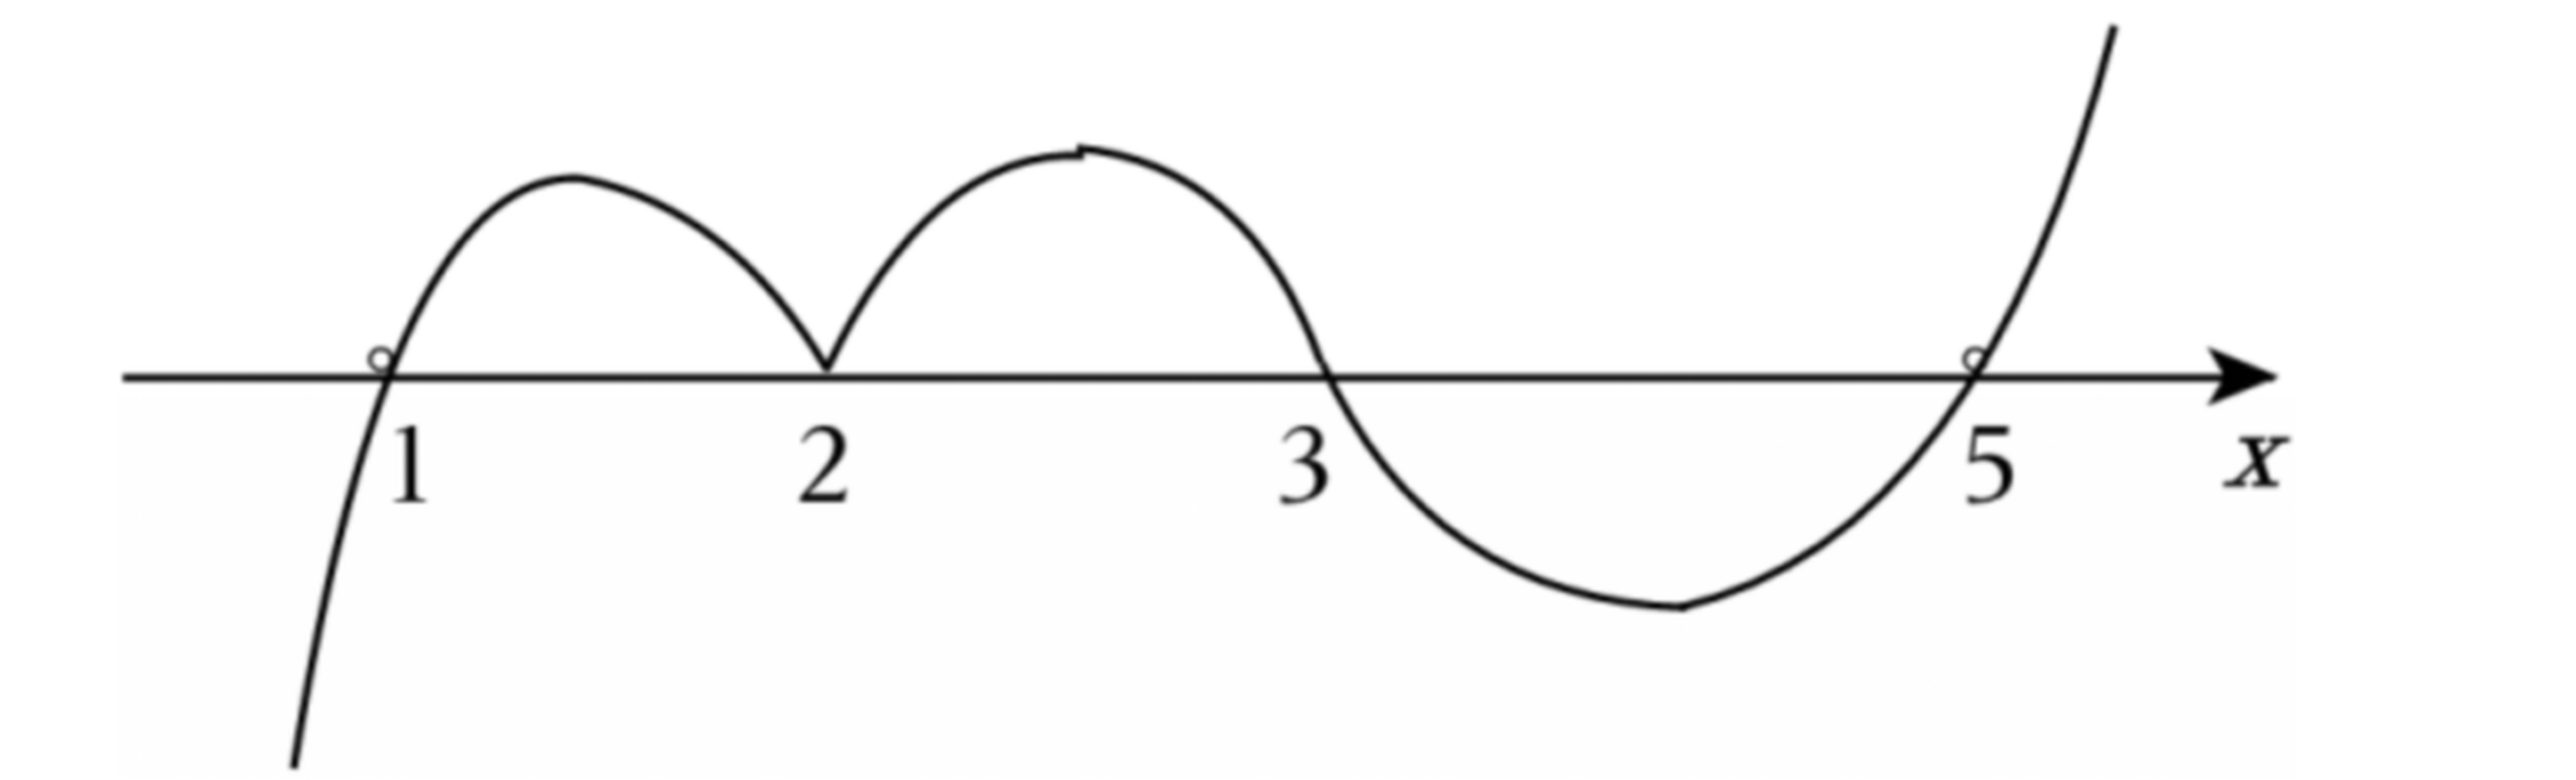
\includegraphics[width=0.62\textwidth]{figures/gao145_q16_a3.png}
\end{center}
\step{得不等式的解集为 $\{x\mid x<1\text{ 或 }x=2\text{ 或 }3\leqslant x<5\}$，}
\step{对应的正整数解为 $2$，$3$，$4$，满足题意，故排除 $B$、$D$；}
\step{当 $a=7$ 时，}
\begin{center}
% a=7 数轴标根图取 06 页，去粉色水印、去色、4× LANCZOS 放大；仅答案版出
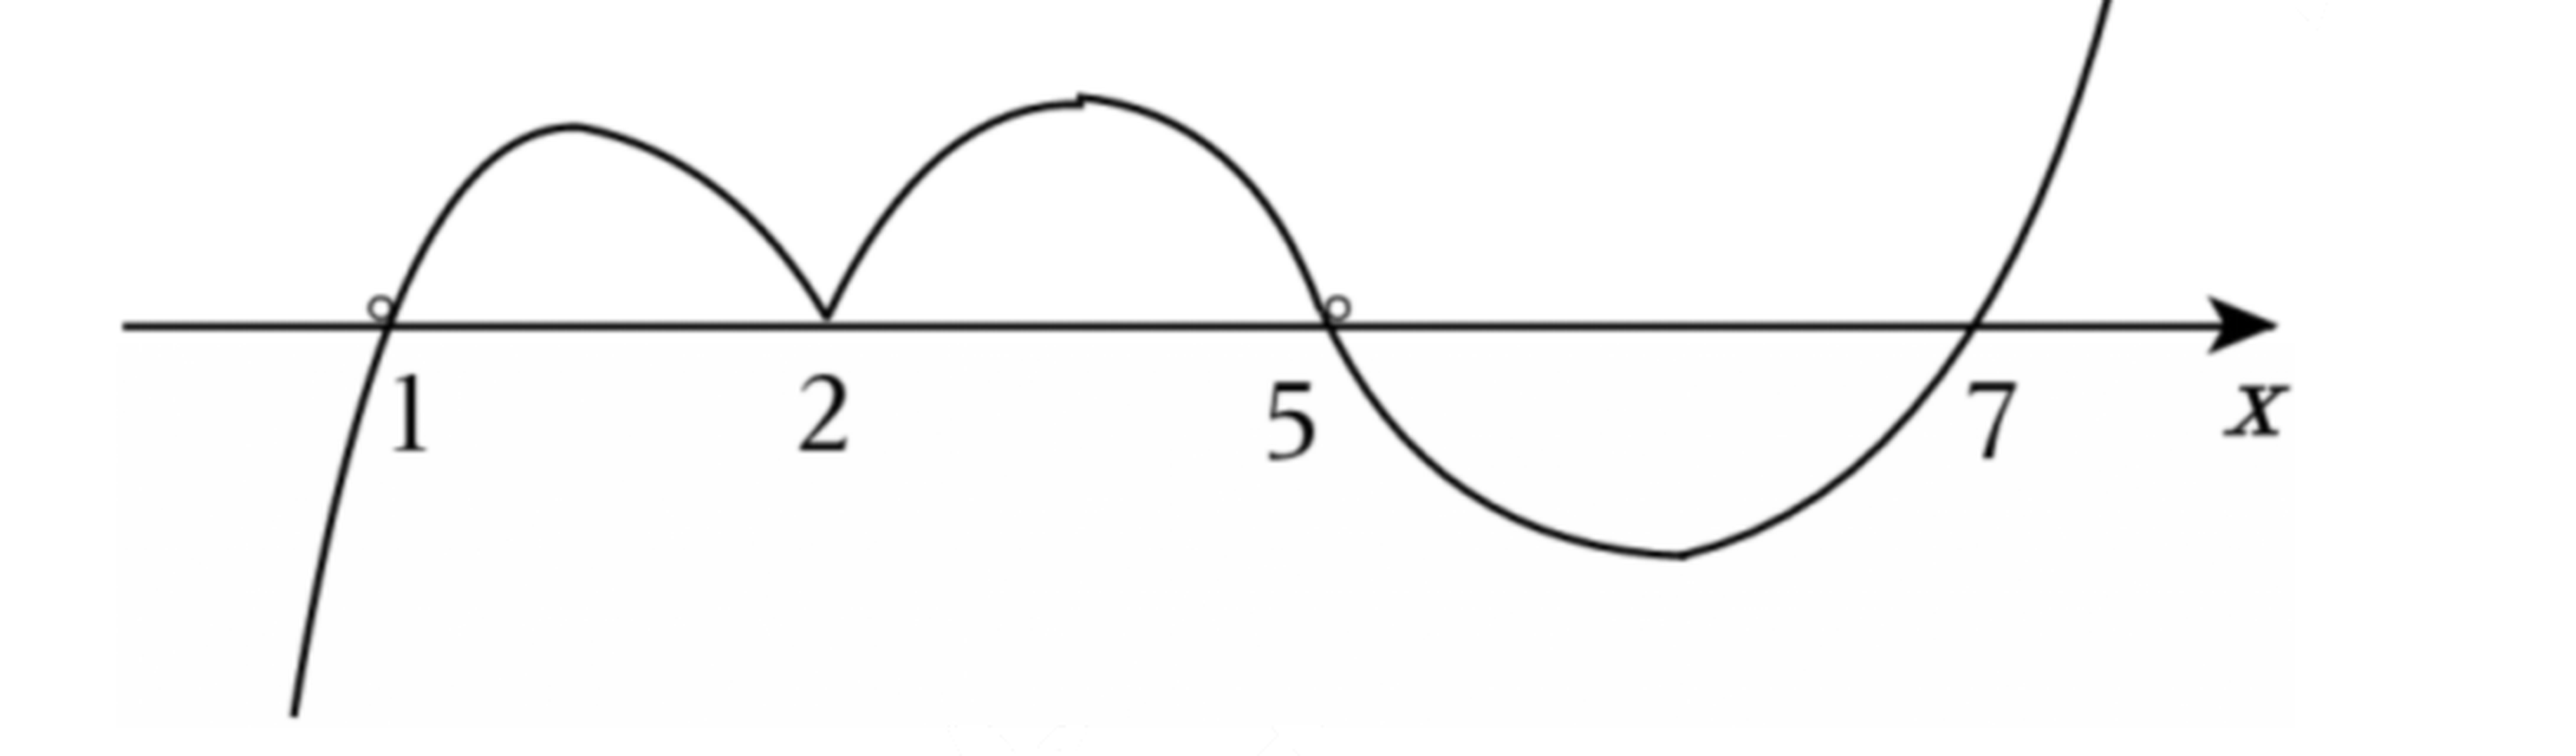
\includegraphics[width=0.62\textwidth]{figures/gao145_q16_a7.png}
\end{center}
\step{得不等式的解集为 $\{x\mid x<1\text{ 或 }x=2\text{ 或 }5<x\leqslant7\}$，}
\step{对应的正整数解为 $2$，$6$，$7$，满足题意，故 $A$ 正确，$C$ 错误.}
\step{故选 $A$.}
\solend
\fi

\end{enumerate}

\bigsec{三、解答题}

\begin{enumerate}
\setcounter{enumi}{16}

% 第 17 题：题干在 06 页、解析续至 07 页，按印刷行断，共 7 行；
% "lg(10÷5)" 的除号照录 \div
\item (1) 已知 $a+a^{-1}=6$，求 $a^2+a^{-2}$ 及 $a^{\frac12}-a^{-\frac12}$ 的值；

(2) 已知 $\lg5=a$，$\lg6=b$，用 $a$、$b$ 分别表示 $\lg2$、$\lg3$、$\lg300$ 和 $\log_{12}15$.

\ifanswer
\solbegin
\step{(1) 因为 $a+a^{-1}=6$，}
\step{所以 $a^2+a^{-2}=(a+a^{-1})^2-2\cdot a\cdot a^{-1}=6^2-2=34$，}
\step{因为 $\left(a^{\frac12}-a^{-\frac12}\right)^2=a-2+a^{-1}=6-2=4$，所以 $a^{\frac12}-a^{-\frac12}=\pm2$；}
\step{(2) $\lg2=\lg(10\div5)=\lg10-\lg5=1-a$，}
\step{$\lg3=\lg(6\div2)=\lg6-\lg2=b-(1-a)=a+b-1$，}
\step{$\lg300=\lg(3\times10^2)=\lg3+\lg10^2=a+b-1+2=a+b+1$，}
\step{所以 $\log_{12}15=\dfrac{\lg15}{\lg12}=\dfrac{\lg3+\lg5}{\lg3+\lg2^2}=\dfrac{a+b-1+a}{a+b-1+2(1-a)}=\dfrac{2a+b-1}{b-a+1}$.}
\solend
\fi

% 第 18 题：题干在 07 页、解析续至 08 页（2 问、分类讨论很长），按印刷行断共 25 行；
% 本卷 Q18 用"图像"（Q13/Q14 用"图象"），逐处照录不统一
\item 已知 $f(x)=(m^2-3m+1)x^{m^2-4m-1}$，$y=f(x)$ 为幂函数且在 $(0,+\infty)$ 上是严格减函数.

(1) 求实数 $m$ 的值以及相应的函数表达式；

(2) 若 $y=f(x)$ 的图像关于 $y$ 轴对称，解关于 $x$ 的不等式 $(x+2)^{1-m}<(3x-1)^{1-m}$.

\ifanswer
\solbegin
\step{(1) 由幂函数的定义得 $m^2-3m+1=1$，}
\step{整理得 $m^2-3m=0$，解得 $m=0$ 或 $m=3$，}
\step{由于 $y=f(x)$ 在 $(0,+\infty)$ 上为严格减函数，}
\step{因此幂函数的指数需满足 $m^2-4m-1<0$，}
\step{当 $m=3$ 时，指数为 $3^2-4\times3-1=-4<0$，满足严格递减条件，}
\step{此时函数表达式为 $f(x)=x^{-4}$，}
\step{当 $m=0$ 时，指数为 $0^2-4\times0-1=-1<0$，满足严格递减条件，}
\step{此时函数表达式为 $f(x)=x^{-1}$，}
\step{所以满足条件的实数 $m$ 为 $0$ 或 $3$，}
\step{对应的函数表达式分别为 $f(x)=x^{-1}$、$f(x)=x^{-4}$；}
\step{(2) 函数图像关于 $y$ 轴对称即函数为偶函数，}
\step{对于 $f(x)=x^{-1}=\dfrac1x$，定义域为 $(-\infty,0)\cup(0,+\infty)$，}
\step{满足 $f(-x)=-f(x)$，为奇函数，图像关于原点对称，}
\step{不满足关于 $y$ 轴对称的条件；}
\step{对于 $f(x)=x^{-4}=\dfrac{1}{x^4}$，定义域为 $(-\infty,0)\cup(0,+\infty)$，}
\step{满足 $f(-x)=f(x)$，为偶函数，图像关于 $y$ 轴对称，}
\step{因此符合条件的 $m$ 值为 $3$，}
\step{将 $m=3$ 代入关于 $x$ 的不等式 $(x+2)^{1-m}<(3x-1)^{1-m}$，}
\step{得 $(x+2)^{1-3}<(3x-1)^{1-3}$，即 $(x+2)^{-2}<(3x-1)^{-2}$，}
\step{因为负指数幂的底数不能为 $0$，所以 $x+2\ne0$ 且 $3x-1\ne0$，}
\step{即 $x\ne-2$ 且 $x\ne\dfrac13$，}
\step{不等式可变形为 $\dfrac{1}{(x+2)^2}<\dfrac{1}{(3x-1)^2}$，}
\step{整理得 $(3x-1)^2<(x+2)^2$，即 $8x^2-10x-3<0$，}
\step{解得 $-\dfrac14<x<\dfrac32$，又 $x\ne-2$ 且 $x\ne\dfrac13$，}
\step{所以不等式的解集为 $\left(-\dfrac14,\dfrac13\right)\cup\left(\dfrac13,\dfrac32\right)$.}
\solend
\fi

% 第 19 题：题干在 08 页、解析续至 09 页，按印刷行断，共 14 行；
% 判别式 cases 块内"△=4a²−16a<0"原卷印扁等边三角 \triangle
%（放大 09 页 zz09_delta.png 与 Q12 高 \Delta 并排确认），逐处照录不统一
\item 已知 $f(x)=ax^2+2ax+4$，$a\in\R$.

(1) 若关于 $x$ 的不等式 $f(x)>0$ 在实数集 $\R$ 上恒成立，求实数 $a$ 的取值范围；

(2) 当 $a<0$ 时，解关于 $x$ 的不等式 $f(x)>(a+1)x+5$.

\ifanswer
\solbegin
\step{(1) 由题意得，关于 $x$ 的不等式 $f(x)>0$ 在实数集 $\R$ 上恒成立，}
\step{即 $ax^2+2ax+4>0$ 在实数集 $\R$ 上恒成立，}
\step{当 $a=0$ 时，不等式为 $4>0$ 恒成立，符合题意；}
\step{当 $a\ne0$ 时，则 $\begin{cases}a>0\\\triangle=4a^2-16a<0\end{cases}$，解得 $0<a<4$.}% 判别式原卷印扁等边三角 $\triangle$，照录
\step{综上所述，实数 $a$ 的取值范围为 $[0,4)$.}
\step{(2) $f(x)=ax^2+2ax+4$，}
\step{当 $a<0$ 时，不等式 $f(x)>(a+1)x+5$ 即为 $ax^2+(a-1)x-1>0$，}
\step{即 $(ax-1)(x+1)>0$，即 $\left(x-\dfrac1a\right)(x+1)<0$，}
\step{当 $a<-1$，即 $\dfrac1a>-1$ 时，解得 $-1<x<\dfrac1a$；}
\step{当 $a=-1$，即 $\dfrac1a=-1$ 时，解得 $x\in\varnothing$；}
\step{当 $-1<a<0$，即 $\dfrac1a<-1$ 时，解得 $\dfrac1a<x<-1$.}
\step{综上所述，当 $a<-1$ 时，不等式的解集为 $\left\{x\mid -1<x<\dfrac1a\right\}$；}
\step{当 $a=-1$ 时，不等式的解集为 $\varnothing$；}
\step{当 $-1<a<0$ 时，不等式的解集为 $\left\{x\mid \dfrac1a<x<-1\right\}$.}
\solend
\fi

% 第 20 题：菜园靠墙图为题目配图（三版都出），题干写"如图"；
% 题干在 09 页（含图）、解析续至 10 页，按印刷行断，共 13 行
\needvspace{8cm}
\item 如图，某人计划用篱笆围成一个一边靠墙（墙足够长）的矩形菜园. 设菜园的长为 $x$ 米，宽为 $y$ 米.

\begin{center}
% 矩形菜园靠墙图取 09 页右下，去粉色水印、去色、4× LANCZOS 放大
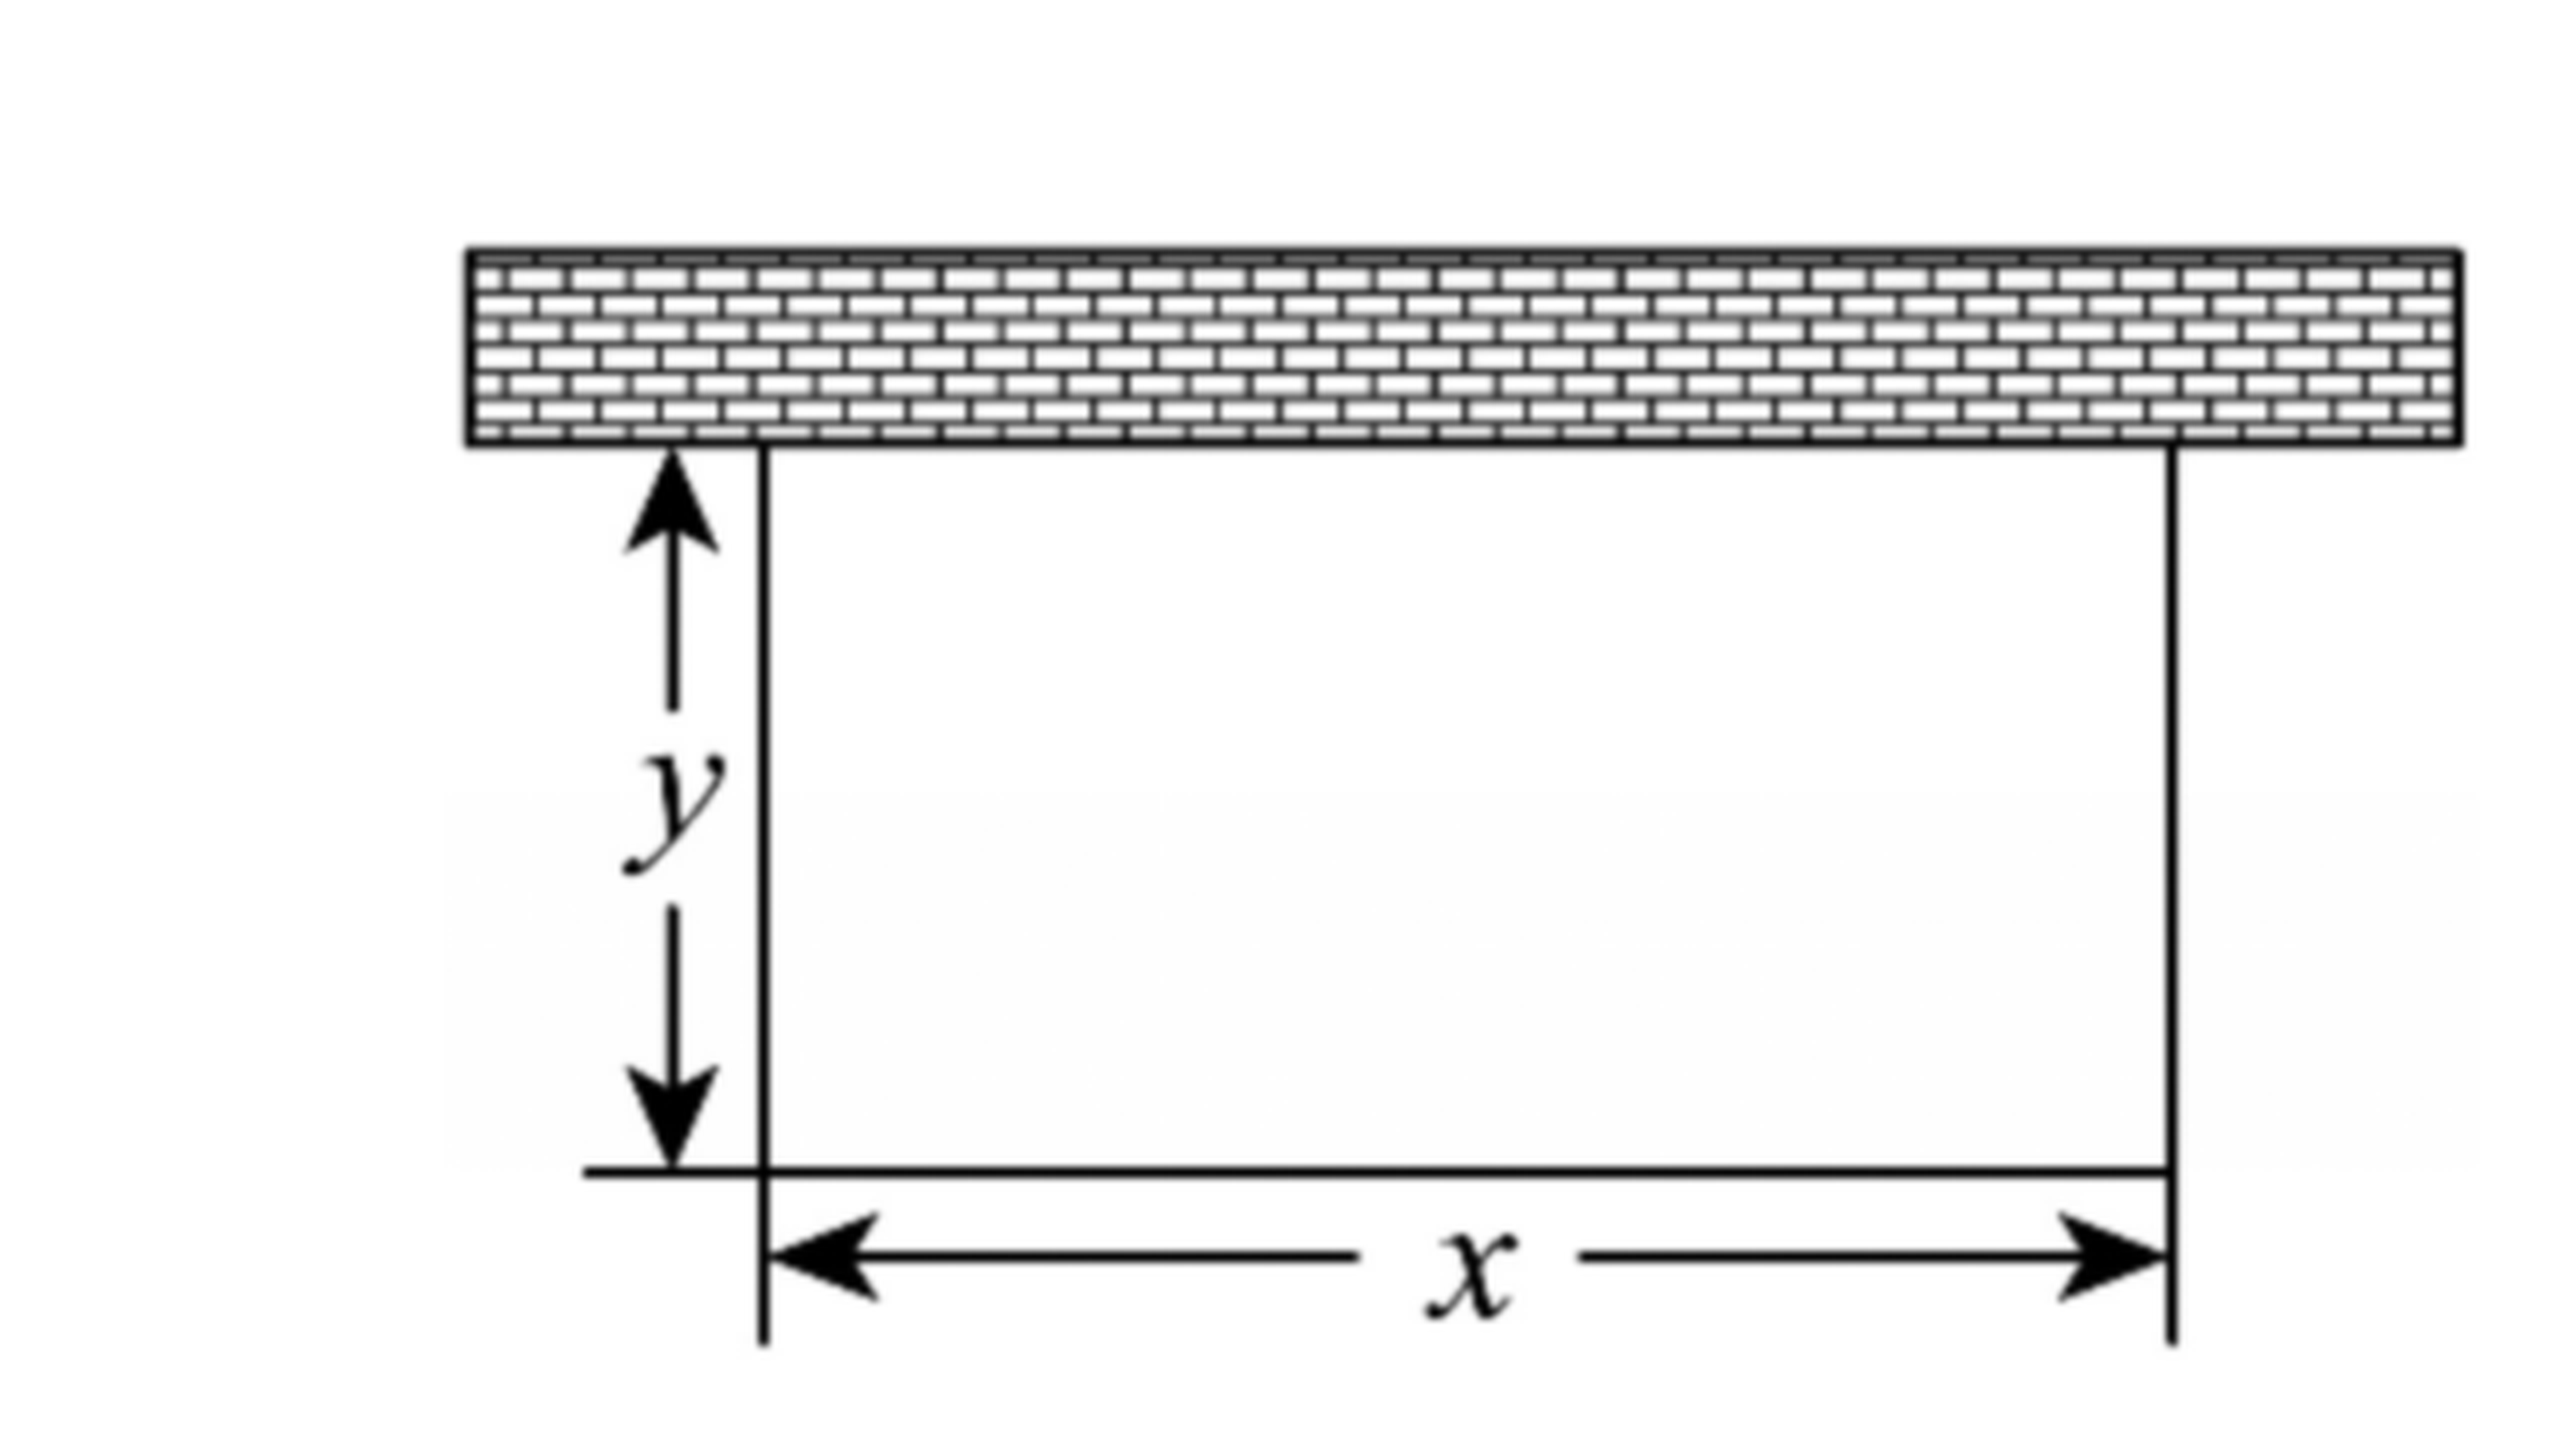
\includegraphics[width=0.55\textwidth]{figures/gao145_q20.png}
\end{center}

(1) 若菜园面积为 72 平方米，则 $x$、$y$ 为何值时，所用篱笆总长最小？

(2) 若 $x$、$y$ 满足 $x+y-xy+63=0$，则菜园面积最小为多少平方米？

\ifanswer
\solbegin
\step{(1) 由题意得，菜园的面积 $S=xy=72$，且 $x>0$，$y>0$，}
\step{所用篱笆总长 $L=x+2y$，}
\step{由基本不等式得 $x+2y\geqslant2\sqrt{x\cdot2y}=2\sqrt{2xy}=2\sqrt{2\times72}=24$，}
\step{当且仅当 $x=2y$ 时取等号，}
\step{联立 $\begin{cases}xy=72\\x=2y\end{cases}$，解得 $\begin{cases}x=12\\y=6\end{cases}$，}
\step{所以当 $x=12$，$y=6$ 时，所用篱笆总长最小；}
\step{(2) 由题意得 $x>0$，$y>0$，且满足 $x+y-xy+63=0$，即 $x+y=xy-63$，}
\step{由基本不等式得 $x+y\geqslant2\sqrt{xy}$，当且仅当 $x=y$ 时取等号，}
\step{所以 $xy-63\geqslant2\sqrt{xy}$. 令 $t=\sqrt{xy}(t>0)$，则 $xy=t^2$，}
\step{上述不等式可化为 $t^2-2t-63\geqslant0$，即 $(t-9)(t+7)\geqslant0$，}
\step{因为 $t>0$，所以 $t+7>0$，故 $t-9\geqslant0$，解得 $t\geqslant9$，所以 $\sqrt{xy}\geqslant9$，}
\step{即 $xy\geqslant81$，当且仅当 $x=y=9$ 时取等号，此时满足 $9+9-81+63=0$，}
\step{所以菜园面积最小为 81 平方米.}
\solend
\fi

% 第 21 题：题干在 10 页、解析续至 11 页（3 问、分类讨论很长），按印刷行断共 22 行；
% 末行"故第 2026 个元素是 2700 之后第一个属于 A 的数，即 2701." 为全卷收尾，
% 无 Q22/Q23、无附加题节；数集 Z/N* 按全稿惯例改 \Z/\N^*
\item 已知集合 $A=\{x\mid x=m^2-n^2$，$m$、$n\in\Z\}$.

(1) 求证：任何奇数 $2k+1(k\in\Z)$ 都是集合 $A$ 中的元素；

(2) 判断偶数 $4k-2(k\in\Z)$ 是否为集合 $A$ 的元素？请说明理由；

(3) 若将集合 $A$ 中的正整数由小到大排列，求出集合 $A$ 中第 2026 个正整数.

\ifanswer
\solbegin
\step{(1) 因为 $x=(k+1)^2-k^2=2k+1(k\in\Z)$，}
\step{所以任何奇数 $2k+1(k\in\Z)$ 都属于集合 $A$；}
\step{(2) 偶数 $4k-2(k\in\Z)$ 不是集合 $A$ 的元素，理由如下：}
\step{由题意得 $x=m^2-n^2=(m-n)(m+n)$，}
\step{当 $m$、$n$ 均为奇数时，设 $m=2k_1+1$，$n=2k_2+1(k_1$、$k_2\in\Z)$，}
\step{则 $m^2-n^2=(2k_1+1)^2-(2k_2+1)^2=(2k_1-2k_2)(2k_1+2k_2+2)$}
\step{$=4(k_1-k_2)(k_1+k_2+1)$，}
\step{因为 $k_1$、$k_2\in\Z$，所以 $k_1-k_2\in\Z$，$k_1+k_2+1\in\Z$，}
\step{从而 $m^2-n^2$ 为 $4$ 的倍数；}
\step{当 $m$、$n$ 均为偶数时，设 $m=2k_1$，$n=2k_2(k_1$、$k_2\in\Z)$，}
\step{$m^2-n^2=4k_1^2-4k_2^2=4(k_1^2-k_2^2)$ 为 $4$ 的倍数；}
\step{当 $m$、$n$ 为一个偶数一个奇数时，不妨设 $m$ 为偶数，$n$ 为奇数，}
\step{设 $m=2k_1$，$n=2k_2+1(k_1$、$k_2\in\Z)$，}
\step{则 $m^2-n^2=4k_1^2-(2k_2+1)^2=4(k_1^2-k_2^2-k_2)-1$ 为奇数.}
\step{无论哪种情况均不满足 $4k-2(k\in\Z)$，}
\step{故偶数 $4k-2(k\in\Z)$ 不是集合 $A$ 的元素；}
\step{(3) 由前两问得，$4$ 的倍数和奇数属于集合 $A$ 中的元素，}
\step{令集合 $A$ 中的正整数元素为 $4k-3$、$4k-1$、$4k(k\in\N^*)$，}
\step{对任意的 $k\in\N^*$，连续的 $4$ 个整数 $4k-3$、$4k-2$、$4k-1$、$4k$ 中}
\step{有三个数 $4k-3$、$4k-1$、$4k$ 都在集合 $A$ 中，}
\step{因为 $2026=3\times675+1$，所以集合 $A$ 中第 $2025$ 个元素为 $4\times675=2700$，}
\step{故第 2026 个元素是 2700 之后第一个属于 $A$ 的数，即 2701.}
\solend
\fi

\end{enumerate}

\end{document}
"
%
% ① 原始材料：微信公众号"魔都数学加油站"文章，连载"27学年高一145"，原文标题
% "27学年高一145——2026-2027年上海市市二中学高一上期中"；
% 原文链接：https://mp.weixin.qq.com/s/6V-i9KE0GWodC-wmd5z8nQ 。
% 正文为 11 张 PNG 页（01/02/03/08/10/11 为 4762×6735，04/05/06/07/09 为 2560×3620，
% 同一篇各页分辨率不同，逐页按各自分辨率裁图核对，别按预览比例换算裁框）。
% 题目下印【答案】或【解析】，为混合体例讲评版：Q3 只印【答案】、无【解析】，其余
% 18 题印【解析】。题目、解析均据原图转录；卷面粉红色水印"魔都数学加油站"及
% 公众号页脚未录入。
% 全卷插图情况（逐页通读 11 页确认，题干写"如图"处均配有图）：
%   · Q14 韦恩图（05 页右侧，全集 U 矩形＋两圆 M/N＋白色交集、灰色阴影＋U/M/N 标注）：
%     题目配图（选择题选项旁），三版都出，裁自 05 页去水印去色 4× 放大存
%     figures/gao145_q14.png；
%   · Q16 两幅数轴标根波浪曲线（06 页，a=3 与 a=7 各一幅，标根法画
%     (x-1)(x-2)^2(x-5)(x-a)≤0 的符号曲线）：【解析】内的配图，仅答案版出，
%     裁 figures/gao145_q16_a3.png / figures/gao145_q16_a7.png（或合并一张），
%     放在答案版条件块内 \solbegin 的 \step 之间（照 高一73 第 16 题成例）；
%   · Q20 矩形菜园靠墙图（09 页右下，灰色砖墙＋矩形菜园＋x/y 标注＋箭头）：
%     题目配图，三版都出，裁自 09 页去水印去色 4× 放大存 figures/gao145_q20.png；
%   其余各页逐页确认无其它题目配图、无表格、亦无"题干写如图而源码漏图"一处。
%
% 卷首标题：原卷印作"2026-2027 年市二中学高一上期中"，年份区间按全稿惯例排 en dash；
% 原卷卷面未印副标题，本稿按同期中卷（高一140／141／143／144）知识模块口径补出
% "集合与常用逻辑用语、不等式、函数"。
%
% 题号体例：本卷共 19 题——一、填空题 3—12（10 题）、二、选择题 13—16（4 题）、
% 三、解答题 17—21（5 题）。三节分别 \setcounter{enumi}{2}／{12}／{16}。
% 原卷从第 3 题起、无第 1、2 题，本稿保留原题号；全卷无附加题节。
%
% ② 与原卷的排版差异：
%   ① 原文从第 3 题起，本稿保留原题号；共 19 题三节；
%   ② 混合体例：原卷 Q3 只印【答案】、无【解析】（"第一步应假设___。
%      【答案】x≤2 或 y≤2"），按 高一140 第 5 题成例提 \ans{}、不补造解析；
%      其余 18 题印【解析】，用 \solbegin…\solend，选择题答案在解析末句"故选 X"
%      （Q13 选 B、Q14 选 D、Q15 选 D、Q16 选 A，逐个放大原图核实）、
%      题干括号 \mbox{（\quad）} 留空、不另提 \ans{}；填空／解答答案落在解析里；
%      答案版【答案】/【解析】标记数 = 19（1 个 \ans ＋ 18 个 \solbegin）= 全卷题数；
%   ③ 原卷卷面未印副标题，本稿按知识模块口径补出；
%   ④ 原卷填空横线按全稿惯例排 \blankline[4.4em]；选择题括号排 \mbox{（\quad）}、
%      选项段前按惯例加 \keepwithprev；解答题不留作答区、不加 \anspace
%      （原卷为讲评版，与 129／131／132／133／136／140／141／143／144 同）；
%   ⑤ 数集：Q9"a、b∈R"、Q12"a∈R"、Q21"m、n∈Z""k∈Z""k∈N*"等原卷印
%      斜体或黑板粗体 R/Z/N，按全稿惯例统一改 \R／\Z／\N^*；绝对值排 \lvert…\rvert，
%      集合描述竖线排 \mid；不等号按全稿惯例排 \leqslant／\geqslant；
%      补集照原卷上划线排 \overline{M}／\overline{N}（Q14 选项 B/C/D 逐处核）；
%      空集记号 \varnothing；\subset（单线⊂）与 \subseteq（带下划线⊆）逐处照录不统一；
%   ⑥ 子题标号 (1)(2)(3) 原卷印半角括号照录；圈数字进数学式用 \text{①}（否则 FONTCHK 挂）；
%      \left…\right 不得拆到不同 $…$ 组；cases 块整体算一个印刷行；
%   ⑦ 题干／解析中的中文弯引号按原卷照录（Q3"若 x+y>4，则 x>2 且 y>2"、
%      Q11"a₁/a₂=b₁/b₂""M=N"、选填"充分非必要""必要非充分""充要""既非充分也非必要"
%      等，含引号内空格），注释内一律 ASCII 引号；数学式内 CJK 用 \text{}；
%   ⑧ 半角逗号在数学组之间是全稿惯例、非笔误（如 Q5"x₁+x₂=6，x₁x₂=√3"、
%      Q7"a>1，b>1"、指数／对数式内逗号），逐处照录别改全角；行末西文句点照录为
%      ASCII `.`；行中全角逗号／顿号照录；
%   ⑨ "图像／图象"逐处照录不统一（Q18"图像关于 y 轴对称"等，核全卷）；
%   ⑩ 判别式 Δ/△ 混用是照录项：Q12 解析"Δ=a²−4a²(2a−3)>0"、
%      Q19 解析"Δ=4a²−16a<0"等，放大原图判断是高 \Delta（等腰偏高、高>宽）
%      还是扁 \triangle，逐处照录不得统一（参照 高一142／144 头注④口径）；
%   ⑪ 一条 \step = 原卷解析的一个印刷行，cases 块整体算一个印刷行；别把原卷折行
%      并起来、别把一行拆多条。Q6 分段讨论、Q12 三个 cases 条件组、Q16 数轴标根、
%      Q18／Q19 分类讨论、Q21 三问均按印刷行逐条断，不丢行；
%   ⑫ Q14 韦恩图为"题干＋选项＋图"整块，加 \needvspace 守卫推走（守卫放 \item 之前，
%      见 高一140 Q14、高一144 Q17 成例与切页审计 B 类坑）；Q20 菜园图同理；
%      三版切页审计均"合计异常：无"；
%   ⑬ 跨页续印按题合并：Q3/4/5/6 在 01 页（Q6 解析续 02 页顶）；Q7/8/9/10 在 02 页
%      （Q10 解析续 03 页）；Q11/12 在 03 页（Q12 解析续 04 页，很长）；
%      Q13 在 04 页末、解析在 05 页顶；Q14/15/16 在 05 页（Q16 解析续 06 页含两幅数轴图）；
%      Q17 在 06 页、解析续 07 页；Q18 在 07 页、解析续 08 页；Q19 在 08 页、解析续 09 页；
%      Q20 在 09 页（含菜园图）、解析续 10 页；Q21 在 10 页、解析续 11 页
%      （末页收尾"故第 2026 个元素是 2700 之后第一个属于 A 的数，即 2701."、
%      无 Q22/Q23、无附加题节）。本稿按题连排，不丢行、不并折行；
%   ⑭ 原卷解析内若有红色"法一／法二"之类小标题，按全稿惯例排 \stepm{标签}{…}
%      （黑体着色、不引入红色、不改 common.sty），头注注明；水印"魔都数学加油站"
%      红色不录入。
%
% ③ 行数复核：一条 \step／\stepm = 原卷解析的一个印刷行，cases 块作一个印刷行计。
%   逐题数（主会话逐页核对定稿）：Q3：0（只印【答案】、提 \ans{}，不计入 \step 账）；
%   Q4：3；Q5：2；Q6：10；Q7：3；Q8：3；Q9：2；Q10：7；Q11：4；Q12：12；
%   Q13：2；Q14：2；Q15：4；Q16：9；Q17：7；Q18：25；Q19：14；Q20：13；Q21：22。
%   合计 144 条 \step（本卷无 \stepm：解析内无红色"法一／法二"类小标题），
%   与原卷逐题印刷行相等。全卷 18 题设 \solbegin…\solend ＋ Q3 一处 \ans{}，
%   答案版【答案】/【解析】标记数 = 19 = 全卷题数。
%
% ④ 判别式／子集符号结论（逐处放大原图照录、不得统一，主会话像素级复核）：
%   判别式全卷 2 处、两形混用逐处照录不统一（参照 高一142／144 头注④口径）：
%     · Q12 解析 cases 块"Δ=a²−4a²(2a−3)>0" 原卷印等腰偏高粗三角（高>宽），
%       照录 \Delta（放大 04 页 /tmp/gao145s2/main_q12_delta.png 确认）；
%     · Q19 解析 cases 块"△=4a²−16a<0" 原卷印扁等边空心三角（宽≈高、细线），
%       照录 \triangle（放大 09 页 /tmp/gao145s2/main_q19_delta.png 确认）。
%   子集／补集：Q14 选项 A `M\cup N`、B `M\cap\overline{N}`（上划线只在 N 上）、
%   C `\overline{M\cup N}`（罩整个 M∪N）、D `\overline{M\cap N}`（罩整个 M∩N，
%   非 \overline{M}\cap N；放大 05 页 /tmp/gao145s2/main_q14_opts.png 确认），
%   阴影为灰色区域＝全集减白色交集，答案 D，照录 \overline{M\cap N}；
%   全集卷无 \subset／\subseteq 混用（本卷集合题用 \cup／\cap／\overline{}）；
%   空集 \varnothing（Q19 解析 x∈\varnothing）；数集 \R／\Z／\N^* 归一见 ② ⑤。
%
% ⑤ 存疑照录（放大原图确认，照录未改、正文对应处另有 % 注）：
%   1. Q3 题干"若 x+y>4，则 x>2 且 y>2" 后"时"前留一空格、弯引号内空格照录；
%      该卷混合体例（Q3 只印【答案】、提 \ans{}）见 ② ②。
%   2. Q4／Q5 解析中的"1，3，5 和 6"、"x₁+x₂=6,x₁x₂=√3" 等半角／全角逗号
%      逐处照原卷（放大 01 页确认），数学式内半角逗号为全稿惯例、非笔误。
%   3. Q14 选项 D 上划线罩住整个 M∩N（而非仅罩 M），照录 \overline{M\cap N}。
%   4. Q12 判别式高 \Delta 与 Q19 判别式扁 \triangle 两形混用，逐处照录不统一（见 ④）。
%   全卷除此 4 类外未发现其它笔误／自相矛盾处。
%
% ⑥ 跨页续印按题合并说明：见 ② ⑬。
%
\documentclass[a4paper,11pt]{article}
\usepackage{common}

\begin{document}

\examtitlest[3]{2026--2027 年市二中学高一上期中}{集合与常用逻辑用语、不等式、函数}

\bigsec{一、填空题}

\begin{enumerate}
\setcounter{enumi}{2}

% 第 3 题：原卷只印【答案】、无【解析】（放大 01 页确认），按 高一140 第 5 题成例
% 提 \ans{}、不补造解析；题干中文弯引号与"时"前空格照录
\item 用反证法证明命题：“若 $x+y>4$，则 $x>2$ 且 $y>2$” 时，第一步应假设\blankline[4.4em].

\ifanswer
\ans{$x\leqslant2$ 或 $y\leqslant2$}
\fi

% === Q4 ===
\item 设集合 $M$ 满足 $\{1,3,5,6\}\cup M=\{1,2,3,4,5,6\}$，则满足条件的所有 $M$ 的个数为\blankline[4.4em].

\ifanswer
\solbegin
\step{集合 $M$ 满足 $\{1,3,5,6\}\cup M=\{1,2,3,4,5,6\}$，}
\step{则 $M$ 中必含有 $2$ 和 $4$，$1$，$3$，$5$ 和 $6$ 可以选也可不选，}
\step{则满足条件的所有 $M$ 的数目相当于集合 $\{1,3,5,6\}$ 的子集的个数 $2^4=16$.}
\solend
\fi

% === Q5 ===
\item 已知方程 $x^2-6x+\sqrt3=0$ 的两根为 $x_1$ 和 $x_2$，则 $(x_1-x_2)^2=$\blankline[4.4em].

\ifanswer
\solbegin
\step{因为方程 $x^2-6x+\sqrt3=0$ 的两根为 $x_1$ 和 $x_2$，所以 $x_1+x_2=6,x_1x_2=\sqrt3$，}% 数学式内半角逗号为全稿惯例，照录
\step{所以 $(x_1-x_2)^2=(x_1+x_2)^2-4x_1x_2=36-4\sqrt3$.}
\solend
\fi

% 第 6 题：题干在 01 页，解析续至 02 页顶（末 2 行），按印刷行逐条断，共 10 行
\item 不等式 $\lvert x-2026\rvert+\lvert x-2029\rvert>3$ 的解集是\blankline[4.4em].

\ifanswer
\solbegin
\step{当 $x<2026$ 时，$x-2026<0$，$x-2029<0$，}
\step{原不等式可化为 $(2026-x)+(2029-x)>3$，解得 $x<2026$，}
\step{故此时，不等式的解为 $x<2026$；}
\step{当 $2026\leqslant x\leqslant2029$ 时，$x-2026\geqslant0$，$x-2029\leqslant0$，}
\step{原不等式可化为 $(x-2026)+(2029-x)>3$，即 $3>3$，显然不成立，}
\step{故此时，不等式无解；}
\step{当 $x>2029$ 时，$x-2026>0$，$x-2029>0$，}
\step{原不等式可化为 $(x-2026)+(x-2029)>3$，解得 $x>2029$，}
\step{故此时，不等式的解为 $x>2029$.}
\step{综上，原不等式的解集为 $(-\infty,2026)\cup(2029,+\infty)$.}
\solend
\fi

% === Q7 ===
\item 已知 $a>1$，$b>1$，若 $\log_a b+\log_b a=2$，且 $ab=2$，则 $\log_2(a+b)=$\blankline[4.4em].

\ifanswer
\solbegin
\step{由 $\log_a b+\log_b a=2$，$a>1$，$b>1$，得 $\log_a b+\dfrac{1}{\log_a b}=2$，}
\step{即 $(\log_a b)^2-2\log_a b+1=0$，则 $(\log_a b-1)^2=0$，解得 $\log_a b=1$，即 $a=b$，}
\step{又 $ab=2$，所以 $a=b=\sqrt2$，所以 $\log_2(a+b)=\log_2 2\sqrt2=\log_2 2^{\frac32}=\dfrac32$.}
\solend
\fi

% === Q8 ===
\item 已知 $m>0$，$n>0$，且 $m+n=1$，则 $\dfrac1m+\dfrac4n$ 的最小值为\blankline[4.4em].

\ifanswer
\solbegin
\step{由 $m>0$，$n>0$，$m+n=1$，}
\step{则 $\dfrac1m+\dfrac4n=(m+n)\left(\dfrac1m+\dfrac4n\right)=5+\dfrac nm+\dfrac{4m}n\geqslant5+2\sqrt{\dfrac nm\cdot\dfrac{4m}n}=9$，}
\step{当且仅当 $n=2m=\dfrac23$ 时，上式取得等号，故最小值为 $9$.}
\solend
\fi

% === Q9 ===
\item 已知 $a$、$b\in\R$，且 $3a+2b=1$，则 $8^a+4^b$ 最小值为\blankline[4.4em].

\ifanswer
\solbegin
\step{因为 $3a+2b=1$，所以 $8^a+4^b=2^{3a}+2^{2b}\geqslant2\sqrt{2^{3a+2b}}=2\sqrt2$，}
\step{当且仅当 $3a=2b$ 时取等号，故最小值为 $2\sqrt2$.}
\solend
\fi

% 第 10 题：题干在 02 页、解析续至 03 页顶，按印刷行断，共 7 行
\item 已知关于 $x$ 的不等式 $ax^2+bx+c>0$ 的解集为 $\{x\mid 1<x<2\}$，则关于 $x$ 的不等式 $bx^2-ax+c<0$ 的解集为\blankline[4.4em].

\ifanswer
\solbegin
\step{已知关于 $x$ 的不等式 $ax^2+bx+c>0$ 的解集为 $\{x\mid 1<x<2\}$，}
\step{由解集为 $1<x<2$ 且二次函数在两根之间为正，得 $a<0$，两个根为 $1$，$2$，}
\step{所以 $ax^2+bx+c=a(x-1)(x-2)=ax^2-3ax+2a$，}
\step{比较系数得 $b=-3a$，$c=2a$.}
\step{于是 $bx^2-ax+c=-3ax^2-ax+2a=-a(3x-2)(x+1)$，}
\step{$a<0$，故 $bx^2-ax+c<0$ 等价于 $(3x-2)(x+1)<0$，解得 $-1<x<\dfrac23$，}
\step{故 $bx^2-ax+c<0$ 的解集为 $\left\{x\mid -1<x<\dfrac23\right\}$.}
\solend
\fi

% 第 11 题：题干引号内空格照录（放大 03 页确认），四组选填引号亦同；
% 结论"故为必要非充分条件"照录，解析共 4 个印刷行
\item 设 $a_1$、$b_1$、$a_2$、$b_2$ 均为非零实数，不等式 $a_1x+b_1>0$ 和 $a_2x+b_2>0$ 的解集分别为集合 $M$、$N$，那么 “ $\dfrac{a_1}{a_2}=\dfrac{b_1}{b_2}$ ” 是 “ $M=N$ ” 的\blankline[4.4em]条件（选填 “ 充分非必要 ”、“ 必要非充分 ”、“ 充要 ” 和 “ 既非充分也非必要 ”）.

\ifanswer
\solbegin
\step{当 $a_1=b_1=1$，$a_2=b_2=-1$ 时，满足 $\dfrac{a_1}{a_2}=\dfrac{b_1}{b_2}$，}
\step{但是 $M=N$ 不成立，即充分性不成立；}
\step{若 $M=N$ 时，$\dfrac{a_1}{a_2}=\dfrac{b_1}{b_2}$ 一定成立，即必要性成立.}
\step{故为必要非充分条件.}
\solend
\fi

% 第 12 题：题干在 03 页、解析续至 04 页（很长，含 3 个 cases 条件组），
% 按印刷行逐条断共 12 行；cases 块整体算一个印刷行
\item 已知 $f(x)=\dfrac{ax+3}{x-2}$（常数 $a\in\R$）. 函数 $y=f(x)$ 在区间 $[3,+\infty)$ 上是严格减函数，且函数值不恒为负. 若关于 $x$ 的方程 $f(x)=\dfrac{a}{ax-1}$ 有两个不相等的实数根 $x_1$ 和 $x_2$，则 $a$ 的取值范围是\blankline[4.4em].

\ifanswer
\solbegin
\step{$f(x)=\dfrac{ax+3}{x-2}=a+\dfrac{3+2a}{x-2}$，定义域 $(-\infty,2)\cup(2,+\infty)$，}
\step{由于 $y=f(x)$ 在区间 $[3,+\infty)$ 上是严格减函数，且函数值不恒为负，}
\step{所以 $\begin{cases}3+2a>0\\a+\dfrac{3+2a}{3-2}\geqslant0\end{cases}\Rightarrow a\geqslant-1$，}
\step{若关于 $x$ 的方程 $f(x)=\dfrac{a}{ax-1}$ 有两个不相等的实数根 $x_1$ 和 $x_2$，}
\step{则 $\dfrac{ax+3}{x-2}=\dfrac{a}{ax-1}$，即 $(ax+3)(ax-1)=a(x-2)$，$x\ne2$ 且 $ax-1\ne0$，}
\step{当 $a\ne0$ 且 $a\geqslant-1$ 时，$(ax+3)(ax-1)=a(x-2)$，$x\ne2$ 且 $ax-1\ne0$，}
\step{可化为 $\begin{cases}a^2x^2+ax+2a-3=0\\x\ne2,x\ne\dfrac1a\end{cases}$，}
\step{要使方程有两个不相等的实数根 $x_1$ 和 $x_2$，}
\step{则 $\begin{cases}\Delta=a^2-4a^2(2a-3)>0\\a\geqslant-1\text{且}a\ne0\\4a^2+2a+2a-3\ne0\\a^2\cdot\dfrac1{a^2}+a\cdot\dfrac1a+2a-3\ne0\end{cases}\Rightarrow\begin{cases}a<\dfrac{13}{8}\\a\geqslant-1\text{且}a\ne0\\a\ne\dfrac12\text{且}a\ne-\dfrac32\\a\ne\dfrac12\end{cases}$，}% 判别式原卷印等腰偏高三角 $\Delta$，照录（放大 04 页 zz04_delta.png 确认）
\step{得 $-1\leqslant a<\dfrac{13}{8}$ 且 $a\ne0,a\ne\dfrac12$；}
\step{当 $a=0$ 时，方程无解；}
\step{所以 $a$ 的取值范围是 $[-1,0)\cup\left(0,\dfrac12\right)\cup\left(\dfrac12,\dfrac{13}{8}\right)$.}
\solend
\fi

\end{enumerate}

\bigsec{二、选择题}

\begin{enumerate}
\setcounter{enumi}{12}

% 第 13 题：题干在 04 页末、解析在 05 页顶；"图象"照录（本卷 Q13、Q14 用"图象"）
\item 已知幂函数 $f(x)$ 的图象过点 $\left(7,\dfrac{1}{\sqrt7}\right)$，则 $f(x)=$\mbox{（\quad）}

\keepwithprev
A. $x^{-2}$\qquad B. $x^{-\frac12}$\qquad C. $x^{\frac12}$\qquad D. $x^2$

\ifanswer
\solbegin
\step{设幂函数 $f(x)=x^\alpha(\alpha\in\R)$，因为幂函数的图象过点 $\left(7,\dfrac{1}{\sqrt7}\right)$，}
\step{所以 $7^\alpha=\dfrac{1}{\sqrt7}=7^{-\frac12}$，所以 $\alpha=-\dfrac12$，故 $f(x)=x^{-\frac12}$. 故选 $B$.}
\solend
\fi

% 第 14 题：韦恩图为题目配图（三版都出），"题干＋选项＋图"整块，needvspace
% 守卫放在 \item 之前（Q14 为选择题节内第二题，不会让节标题孤落页末）；
% D 选项上划线罩住整个 M∩N（放大 05 页 zz05_q14D.png 确认，非 \overline{M}\cap N）
\needvspace{9cm}
\item 已知全集 $U$ 和集合 $M$、$N$，用集合语言表示图中的阴影部分，正确的是\mbox{（\quad）}

\keepwithprev
A. $M\cup N$\qquad B. $M\cap\overline{N}$\qquad C. $\overline{M\cup N}$\qquad D. $\overline{M\cap N}$

\begin{center}
% 韦恩图取 05 页右侧，去粉色水印、去色、4× LANCZOS 放大
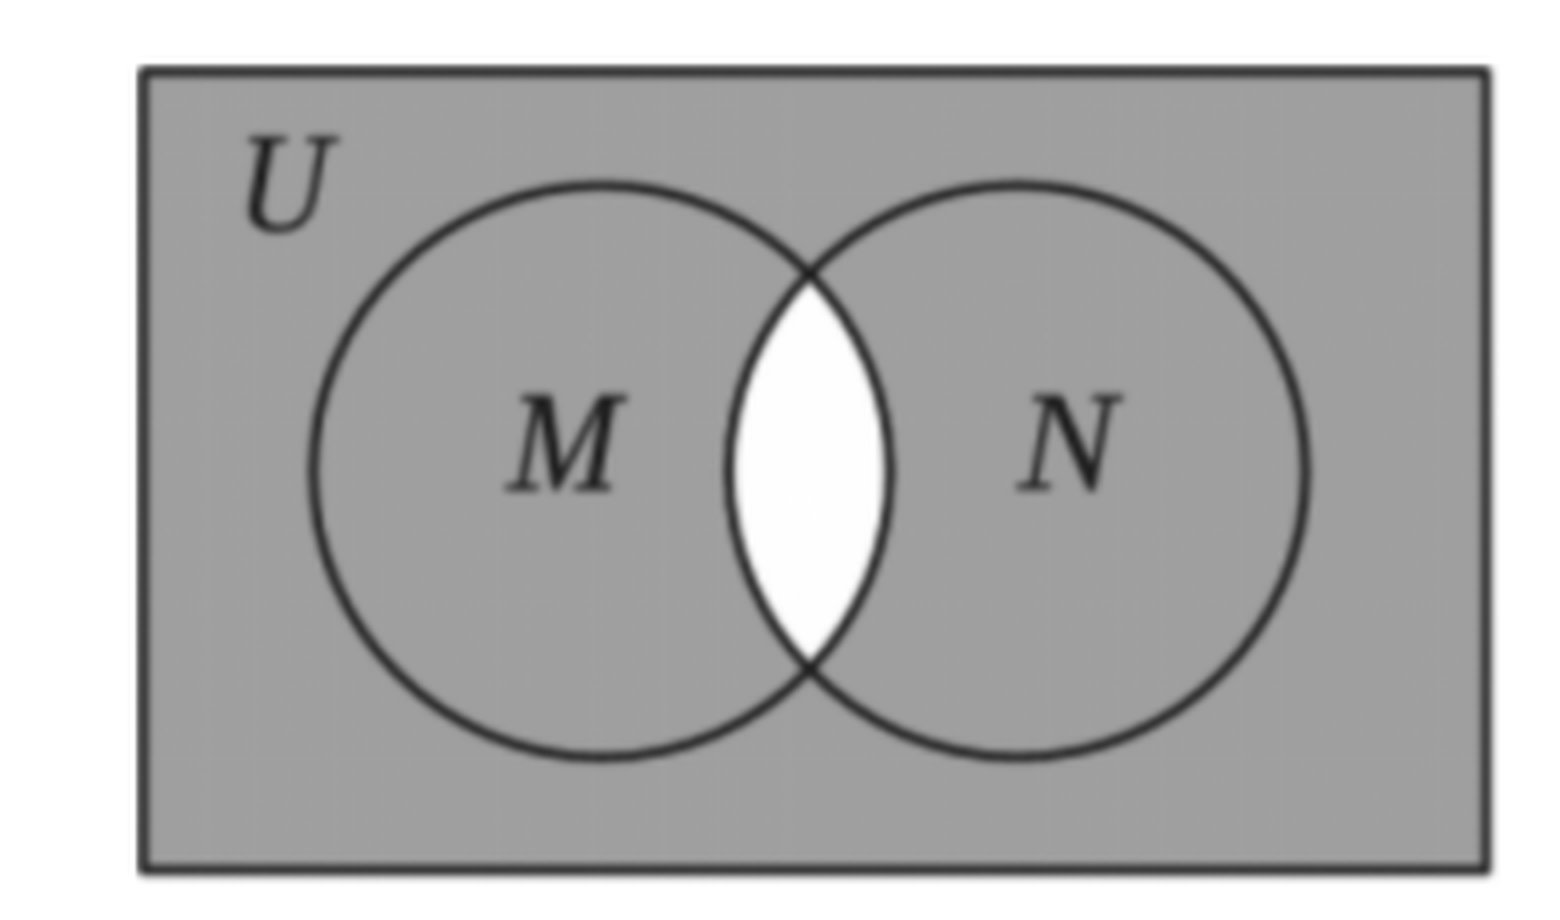
\includegraphics[width=0.40\textwidth]{figures/gao145_q14.png}
\end{center}

\ifanswer
\solbegin
\step{由韦恩图得图中白色区域为集合 $M\cap N$，所以阴影部分表示的集合为 $\overline{M\cap N}$.}
\step{故选 $D$.}
\solend
\fi

% === Q15 ===
\item 已知 $x>-2$，则 $x+\dfrac{1}{x+2}$ 的最小值为\mbox{（\quad）}

\keepwithprev
A. 3\qquad B. 2\qquad C. 1\qquad D. 0

\ifanswer
\solbegin
\step{$x>-2$，则 $x+2>0$，}
\step{所以 $x+\dfrac{1}{x+2}=(x+2)+\dfrac{1}{x+2}-2\geqslant2\sqrt{(x+2)\cdot\dfrac{1}{x+2}}-2=0$，}
\step{当且仅当 $x+2=\dfrac{1}{x+2}$，即 $x=-1$ 时取等号，所以 $x+\dfrac{1}{x+2}$ 的最小值为 $0$.}
\step{故选 $D$.}
\solend
\fi

% 第 16 题：题干在 05 页、解析续至 06 页；两幅数轴标根波浪曲线是【解析】内配图，
% 仅答案版出，放在答案版条件块内 \solbegin 的 \step 之间（照 高一73 第 16 题成例）
\item 关于 $x$ 的不等式 $\dfrac{(x-a)(x-2)^2}{(x-1)(x-5)}\leqslant0$ 的解集中恰有 3 个正整数，则实数 $a$ 的取值范围是\mbox{（\quad）}

\keepwithprev
A. $(-\infty,3]\cup[7,8)$\qquad B. $(-\infty,3)\cup[7,8)$\qquad C. $(-\infty,3]\cup(7,8]$\qquad D. $(-\infty,3)\cup(7,8]$

\ifanswer
\solbegin
\step{由题意，不等式 $\dfrac{(x-a)(x-2)^2}{(x-1)(x-5)}\leqslant0$，}
\step{可化为 $\begin{cases}(x-1)(x-2)^2(x-5)(x-a)\leqslant0\\x\ne1\text{且}x\ne5\end{cases}$，由数轴标根法，}
\step{当 $a=3$ 时，}
\begin{center}
% a=3 数轴标根图取 06 页，去粉色水印、去色、4× LANCZOS 放大；仅答案版出
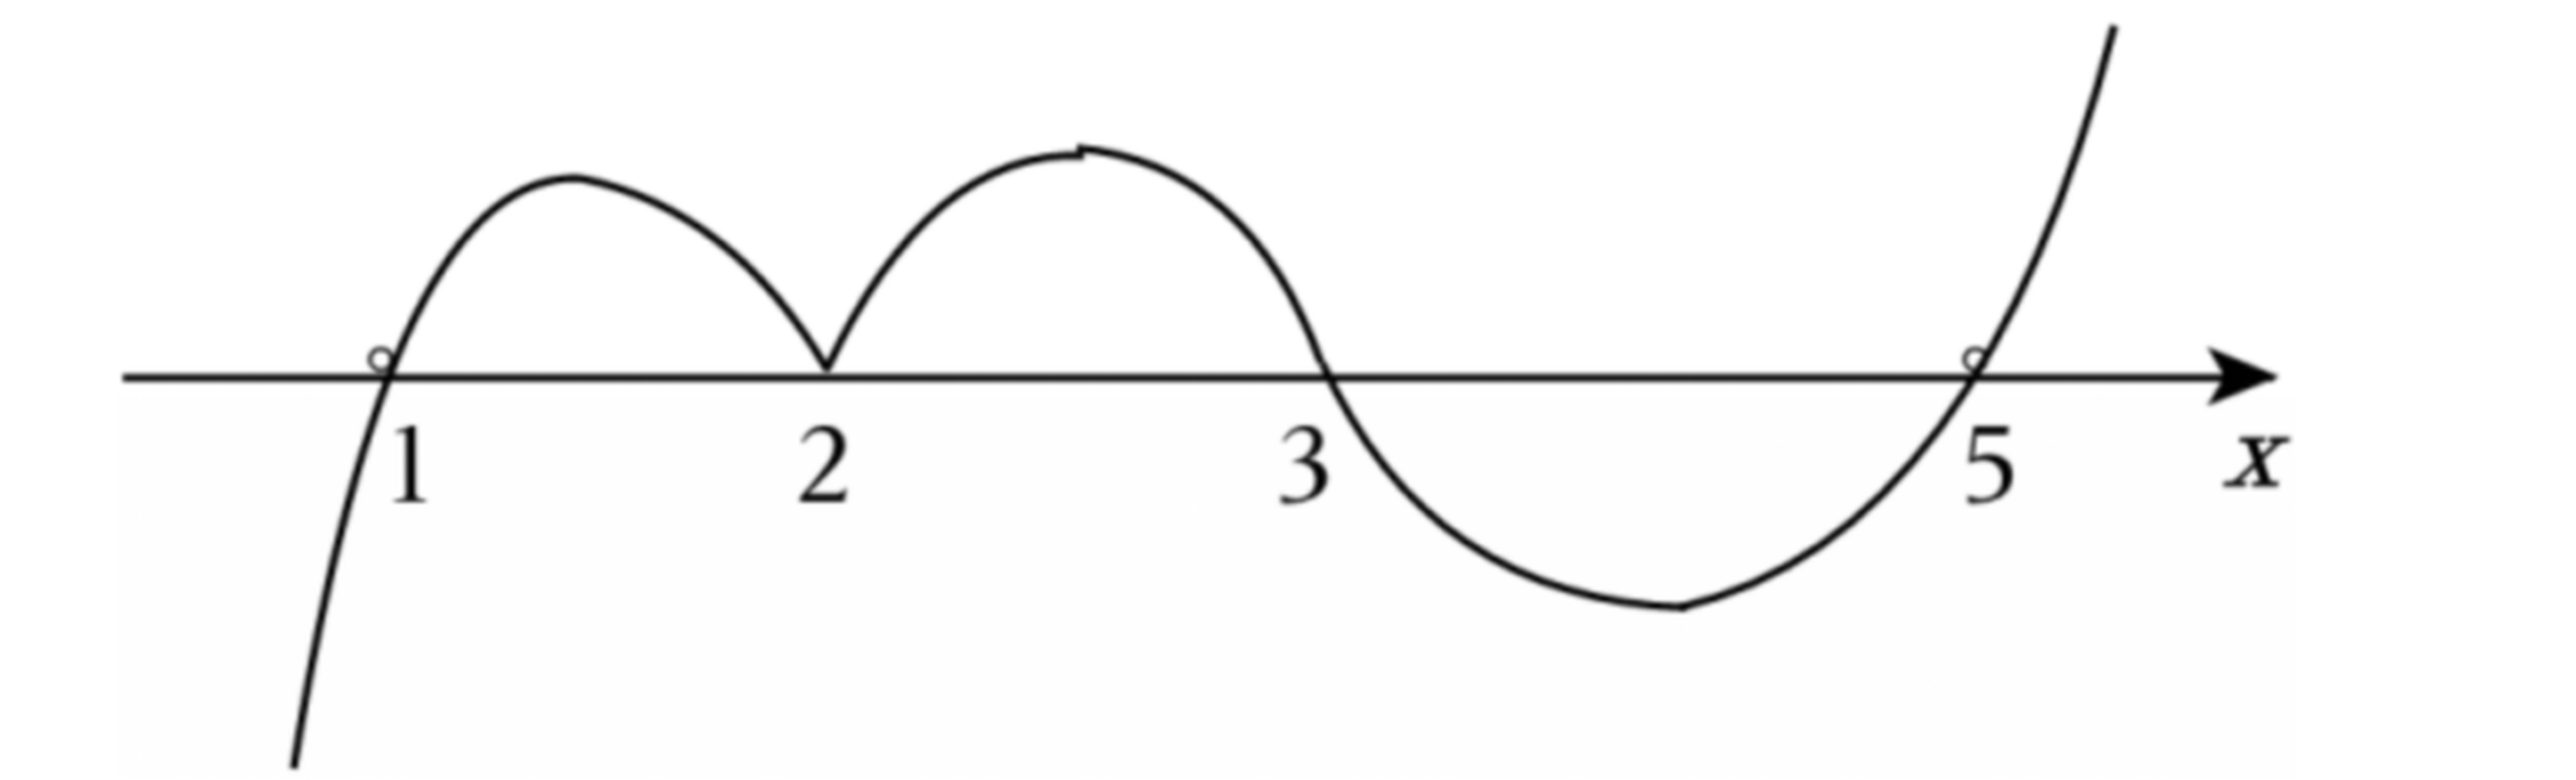
\includegraphics[width=0.62\textwidth]{figures/gao145_q16_a3.png}
\end{center}
\step{得不等式的解集为 $\{x\mid x<1\text{ 或 }x=2\text{ 或 }3\leqslant x<5\}$，}
\step{对应的正整数解为 $2$，$3$，$4$，满足题意，故排除 $B$、$D$；}
\step{当 $a=7$ 时，}
\begin{center}
% a=7 数轴标根图取 06 页，去粉色水印、去色、4× LANCZOS 放大；仅答案版出
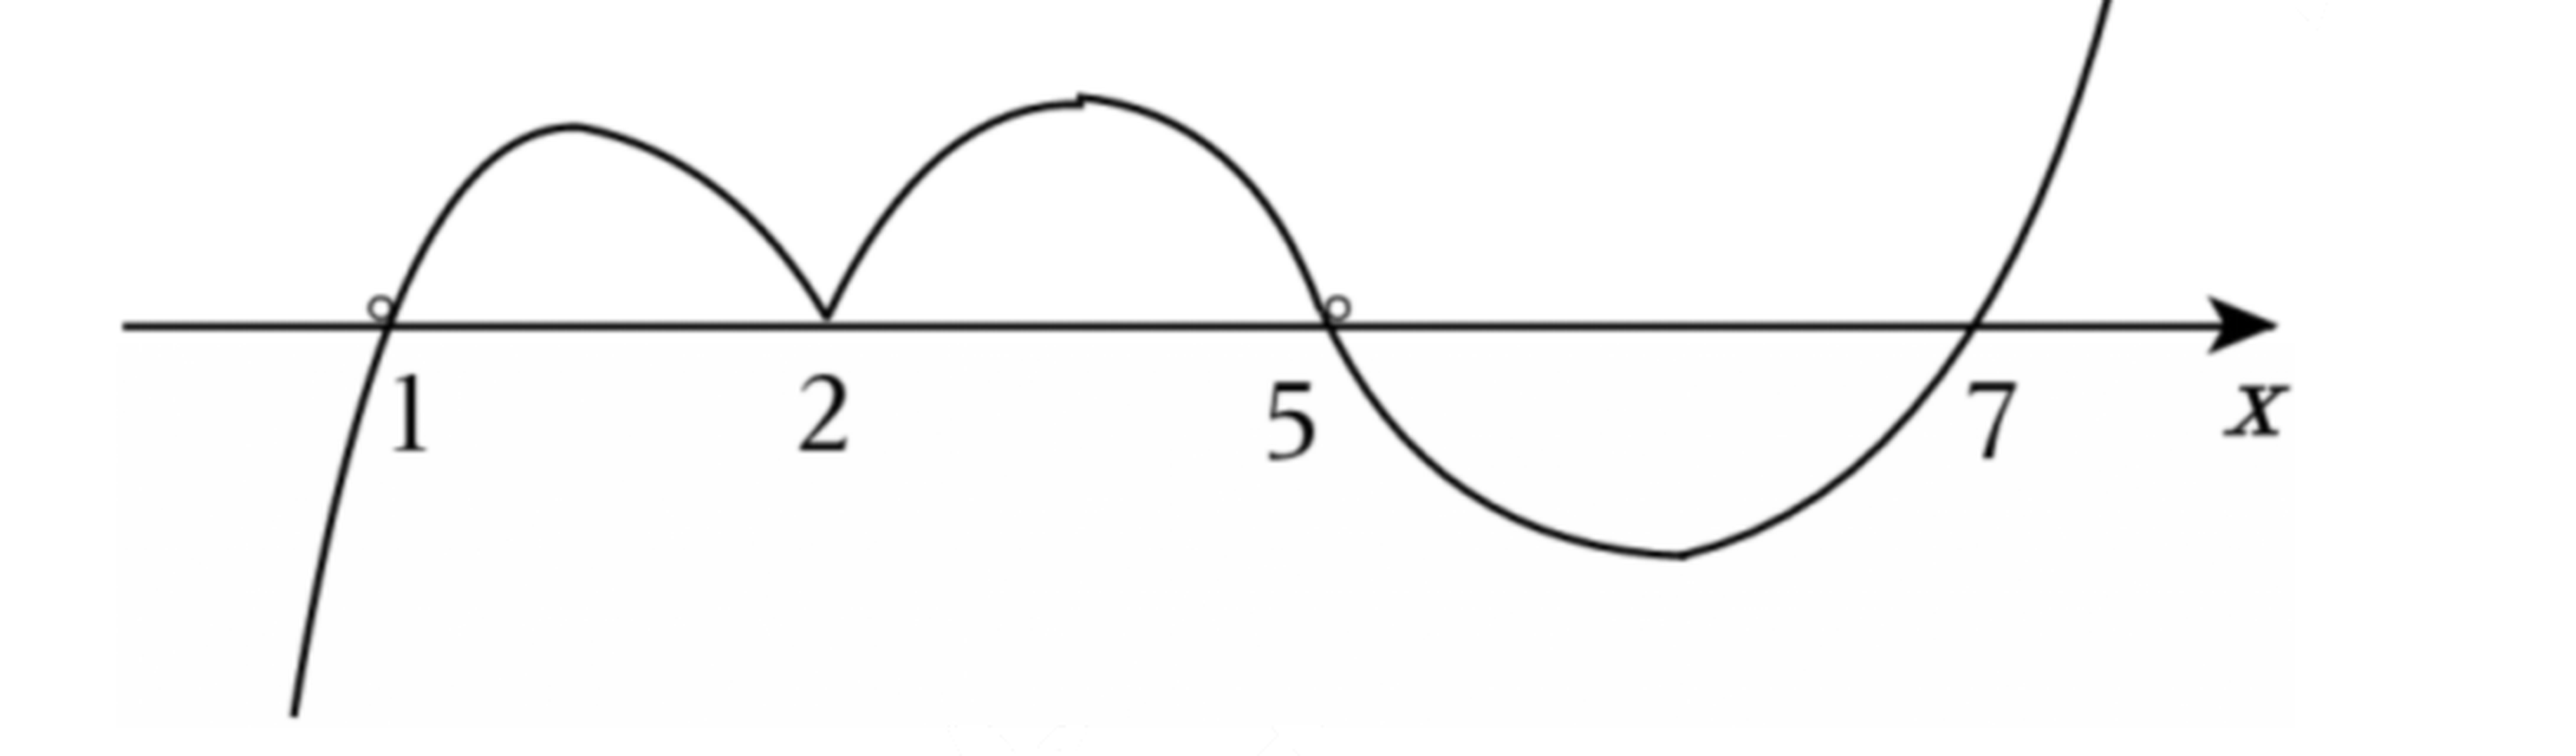
\includegraphics[width=0.62\textwidth]{figures/gao145_q16_a7.png}
\end{center}
\step{得不等式的解集为 $\{x\mid x<1\text{ 或 }x=2\text{ 或 }5<x\leqslant7\}$，}
\step{对应的正整数解为 $2$，$6$，$7$，满足题意，故 $A$ 正确，$C$ 错误.}
\step{故选 $A$.}
\solend
\fi

\end{enumerate}

\bigsec{三、解答题}

\begin{enumerate}
\setcounter{enumi}{16}

% 第 17 题：题干在 06 页、解析续至 07 页，按印刷行断，共 7 行；
% "lg(10÷5)" 的除号照录 \div
\item (1) 已知 $a+a^{-1}=6$，求 $a^2+a^{-2}$ 及 $a^{\frac12}-a^{-\frac12}$ 的值；

(2) 已知 $\lg5=a$，$\lg6=b$，用 $a$、$b$ 分别表示 $\lg2$、$\lg3$、$\lg300$ 和 $\log_{12}15$.

\ifanswer
\solbegin
\step{(1) 因为 $a+a^{-1}=6$，}
\step{所以 $a^2+a^{-2}=(a+a^{-1})^2-2\cdot a\cdot a^{-1}=6^2-2=34$，}
\step{因为 $\left(a^{\frac12}-a^{-\frac12}\right)^2=a-2+a^{-1}=6-2=4$，所以 $a^{\frac12}-a^{-\frac12}=\pm2$；}
\step{(2) $\lg2=\lg(10\div5)=\lg10-\lg5=1-a$，}
\step{$\lg3=\lg(6\div2)=\lg6-\lg2=b-(1-a)=a+b-1$，}
\step{$\lg300=\lg(3\times10^2)=\lg3+\lg10^2=a+b-1+2=a+b+1$，}
\step{所以 $\log_{12}15=\dfrac{\lg15}{\lg12}=\dfrac{\lg3+\lg5}{\lg3+\lg2^2}=\dfrac{a+b-1+a}{a+b-1+2(1-a)}=\dfrac{2a+b-1}{b-a+1}$.}
\solend
\fi

% 第 18 题：题干在 07 页、解析续至 08 页（2 问、分类讨论很长），按印刷行断共 25 行；
% 本卷 Q18 用"图像"（Q13/Q14 用"图象"），逐处照录不统一
\item 已知 $f(x)=(m^2-3m+1)x^{m^2-4m-1}$，$y=f(x)$ 为幂函数且在 $(0,+\infty)$ 上是严格减函数.

(1) 求实数 $m$ 的值以及相应的函数表达式；

(2) 若 $y=f(x)$ 的图像关于 $y$ 轴对称，解关于 $x$ 的不等式 $(x+2)^{1-m}<(3x-1)^{1-m}$.

\ifanswer
\solbegin
\step{(1) 由幂函数的定义得 $m^2-3m+1=1$，}
\step{整理得 $m^2-3m=0$，解得 $m=0$ 或 $m=3$，}
\step{由于 $y=f(x)$ 在 $(0,+\infty)$ 上为严格减函数，}
\step{因此幂函数的指数需满足 $m^2-4m-1<0$，}
\step{当 $m=3$ 时，指数为 $3^2-4\times3-1=-4<0$，满足严格递减条件，}
\step{此时函数表达式为 $f(x)=x^{-4}$，}
\step{当 $m=0$ 时，指数为 $0^2-4\times0-1=-1<0$，满足严格递减条件，}
\step{此时函数表达式为 $f(x)=x^{-1}$，}
\step{所以满足条件的实数 $m$ 为 $0$ 或 $3$，}
\step{对应的函数表达式分别为 $f(x)=x^{-1}$、$f(x)=x^{-4}$；}
\step{(2) 函数图像关于 $y$ 轴对称即函数为偶函数，}
\step{对于 $f(x)=x^{-1}=\dfrac1x$，定义域为 $(-\infty,0)\cup(0,+\infty)$，}
\step{满足 $f(-x)=-f(x)$，为奇函数，图像关于原点对称，}
\step{不满足关于 $y$ 轴对称的条件；}
\step{对于 $f(x)=x^{-4}=\dfrac{1}{x^4}$，定义域为 $(-\infty,0)\cup(0,+\infty)$，}
\step{满足 $f(-x)=f(x)$，为偶函数，图像关于 $y$ 轴对称，}
\step{因此符合条件的 $m$ 值为 $3$，}
\step{将 $m=3$ 代入关于 $x$ 的不等式 $(x+2)^{1-m}<(3x-1)^{1-m}$，}
\step{得 $(x+2)^{1-3}<(3x-1)^{1-3}$，即 $(x+2)^{-2}<(3x-1)^{-2}$，}
\step{因为负指数幂的底数不能为 $0$，所以 $x+2\ne0$ 且 $3x-1\ne0$，}
\step{即 $x\ne-2$ 且 $x\ne\dfrac13$，}
\step{不等式可变形为 $\dfrac{1}{(x+2)^2}<\dfrac{1}{(3x-1)^2}$，}
\step{整理得 $(3x-1)^2<(x+2)^2$，即 $8x^2-10x-3<0$，}
\step{解得 $-\dfrac14<x<\dfrac32$，又 $x\ne-2$ 且 $x\ne\dfrac13$，}
\step{所以不等式的解集为 $\left(-\dfrac14,\dfrac13\right)\cup\left(\dfrac13,\dfrac32\right)$.}
\solend
\fi

% 第 19 题：题干在 08 页、解析续至 09 页，按印刷行断，共 14 行；
% 判别式 cases 块内"△=4a²−16a<0"原卷印扁等边三角 \triangle
%（放大 09 页 zz09_delta.png 与 Q12 高 \Delta 并排确认），逐处照录不统一
\item 已知 $f(x)=ax^2+2ax+4$，$a\in\R$.

(1) 若关于 $x$ 的不等式 $f(x)>0$ 在实数集 $\R$ 上恒成立，求实数 $a$ 的取值范围；

(2) 当 $a<0$ 时，解关于 $x$ 的不等式 $f(x)>(a+1)x+5$.

\ifanswer
\solbegin
\step{(1) 由题意得，关于 $x$ 的不等式 $f(x)>0$ 在实数集 $\R$ 上恒成立，}
\step{即 $ax^2+2ax+4>0$ 在实数集 $\R$ 上恒成立，}
\step{当 $a=0$ 时，不等式为 $4>0$ 恒成立，符合题意；}
\step{当 $a\ne0$ 时，则 $\begin{cases}a>0\\\triangle=4a^2-16a<0\end{cases}$，解得 $0<a<4$.}% 判别式原卷印扁等边三角 $\triangle$，照录
\step{综上所述，实数 $a$ 的取值范围为 $[0,4)$.}
\step{(2) $f(x)=ax^2+2ax+4$，}
\step{当 $a<0$ 时，不等式 $f(x)>(a+1)x+5$ 即为 $ax^2+(a-1)x-1>0$，}
\step{即 $(ax-1)(x+1)>0$，即 $\left(x-\dfrac1a\right)(x+1)<0$，}
\step{当 $a<-1$，即 $\dfrac1a>-1$ 时，解得 $-1<x<\dfrac1a$；}
\step{当 $a=-1$，即 $\dfrac1a=-1$ 时，解得 $x\in\varnothing$；}
\step{当 $-1<a<0$，即 $\dfrac1a<-1$ 时，解得 $\dfrac1a<x<-1$.}
\step{综上所述，当 $a<-1$ 时，不等式的解集为 $\left\{x\mid -1<x<\dfrac1a\right\}$；}
\step{当 $a=-1$ 时，不等式的解集为 $\varnothing$；}
\step{当 $-1<a<0$ 时，不等式的解集为 $\left\{x\mid \dfrac1a<x<-1\right\}$.}
\solend
\fi

% 第 20 题：菜园靠墙图为题目配图（三版都出），题干写"如图"；
% 题干在 09 页（含图）、解析续至 10 页，按印刷行断，共 13 行
\needvspace{8cm}
\item 如图，某人计划用篱笆围成一个一边靠墙（墙足够长）的矩形菜园. 设菜园的长为 $x$ 米，宽为 $y$ 米.

\begin{center}
% 矩形菜园靠墙图取 09 页右下，去粉色水印、去色、4× LANCZOS 放大
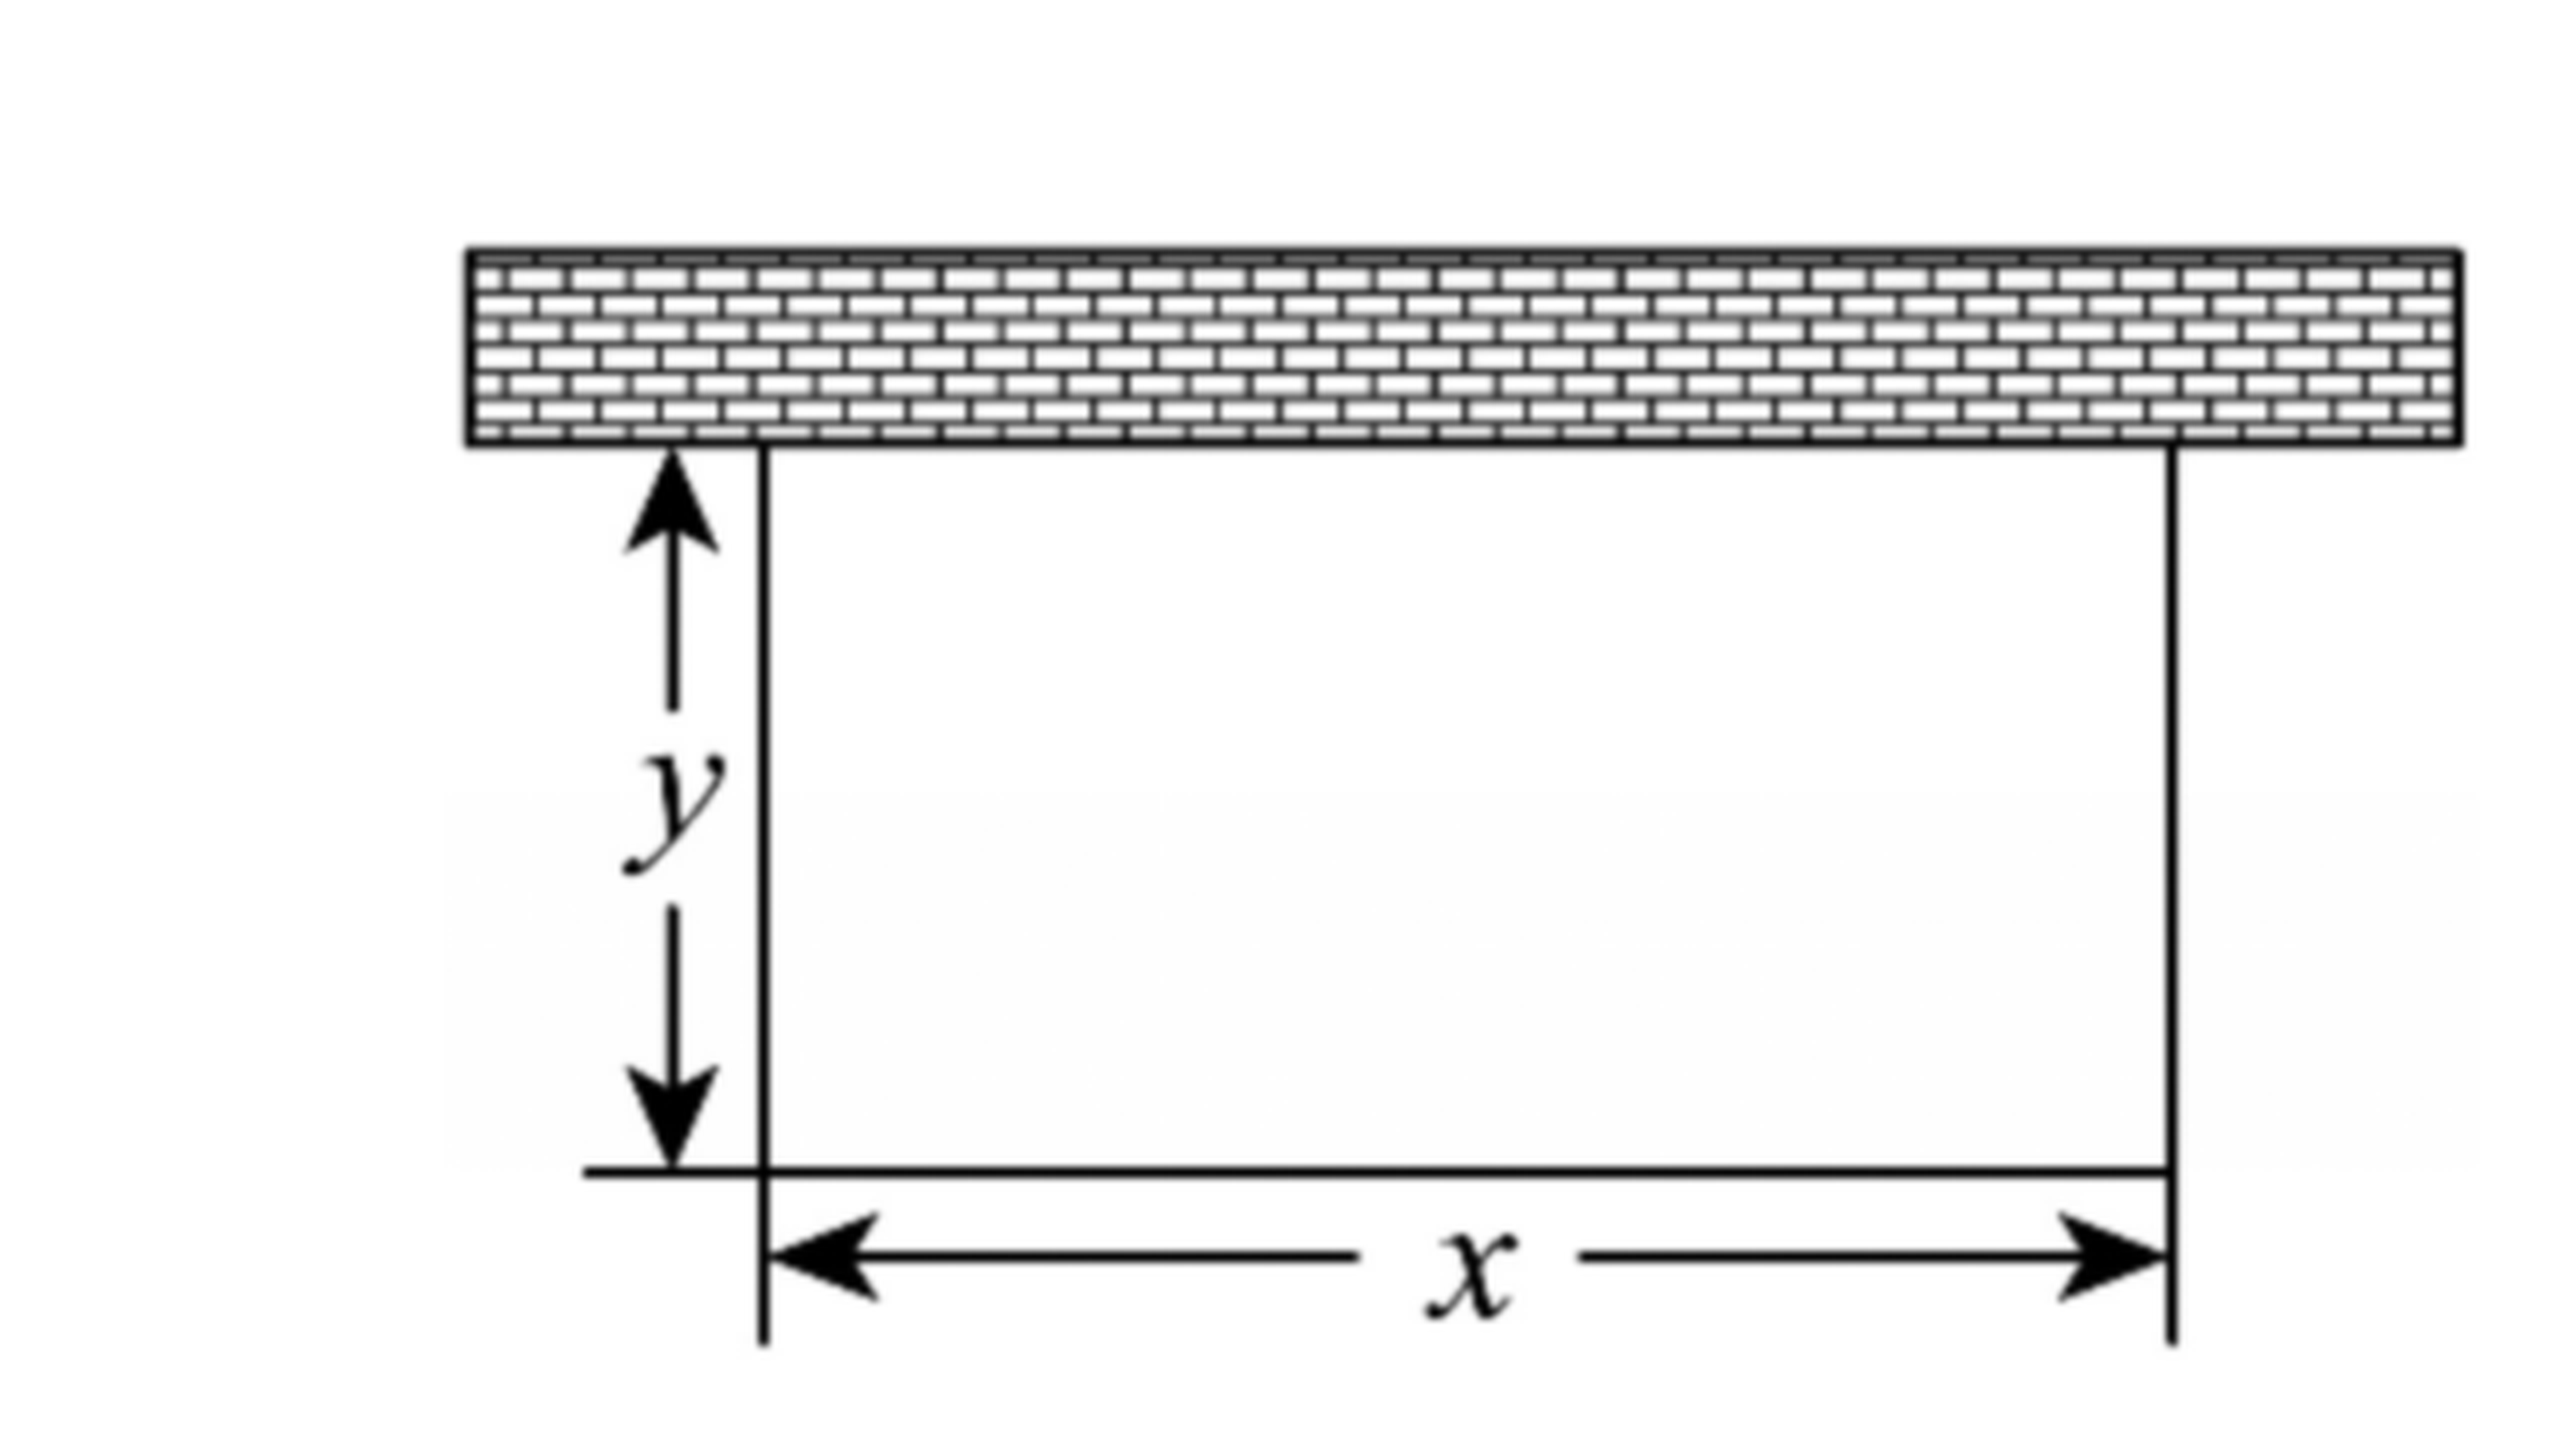
\includegraphics[width=0.55\textwidth]{figures/gao145_q20.png}
\end{center}

(1) 若菜园面积为 72 平方米，则 $x$、$y$ 为何值时，所用篱笆总长最小？

(2) 若 $x$、$y$ 满足 $x+y-xy+63=0$，则菜园面积最小为多少平方米？

\ifanswer
\solbegin
\step{(1) 由题意得，菜园的面积 $S=xy=72$，且 $x>0$，$y>0$，}
\step{所用篱笆总长 $L=x+2y$，}
\step{由基本不等式得 $x+2y\geqslant2\sqrt{x\cdot2y}=2\sqrt{2xy}=2\sqrt{2\times72}=24$，}
\step{当且仅当 $x=2y$ 时取等号，}
\step{联立 $\begin{cases}xy=72\\x=2y\end{cases}$，解得 $\begin{cases}x=12\\y=6\end{cases}$，}
\step{所以当 $x=12$，$y=6$ 时，所用篱笆总长最小；}
\step{(2) 由题意得 $x>0$，$y>0$，且满足 $x+y-xy+63=0$，即 $x+y=xy-63$，}
\step{由基本不等式得 $x+y\geqslant2\sqrt{xy}$，当且仅当 $x=y$ 时取等号，}
\step{所以 $xy-63\geqslant2\sqrt{xy}$. 令 $t=\sqrt{xy}(t>0)$，则 $xy=t^2$，}
\step{上述不等式可化为 $t^2-2t-63\geqslant0$，即 $(t-9)(t+7)\geqslant0$，}
\step{因为 $t>0$，所以 $t+7>0$，故 $t-9\geqslant0$，解得 $t\geqslant9$，所以 $\sqrt{xy}\geqslant9$，}
\step{即 $xy\geqslant81$，当且仅当 $x=y=9$ 时取等号，此时满足 $9+9-81+63=0$，}
\step{所以菜园面积最小为 81 平方米.}
\solend
\fi

% 第 21 题：题干在 10 页、解析续至 11 页（3 问、分类讨论很长），按印刷行断共 22 行；
% 末行"故第 2026 个元素是 2700 之后第一个属于 A 的数，即 2701." 为全卷收尾，
% 无 Q22/Q23、无附加题节；数集 Z/N* 按全稿惯例改 \Z/\N^*
\item 已知集合 $A=\{x\mid x=m^2-n^2$，$m$、$n\in\Z\}$.

(1) 求证：任何奇数 $2k+1(k\in\Z)$ 都是集合 $A$ 中的元素；

(2) 判断偶数 $4k-2(k\in\Z)$ 是否为集合 $A$ 的元素？请说明理由；

(3) 若将集合 $A$ 中的正整数由小到大排列，求出集合 $A$ 中第 2026 个正整数.

\ifanswer
\solbegin
\step{(1) 因为 $x=(k+1)^2-k^2=2k+1(k\in\Z)$，}
\step{所以任何奇数 $2k+1(k\in\Z)$ 都属于集合 $A$；}
\step{(2) 偶数 $4k-2(k\in\Z)$ 不是集合 $A$ 的元素，理由如下：}
\step{由题意得 $x=m^2-n^2=(m-n)(m+n)$，}
\step{当 $m$、$n$ 均为奇数时，设 $m=2k_1+1$，$n=2k_2+1(k_1$、$k_2\in\Z)$，}
\step{则 $m^2-n^2=(2k_1+1)^2-(2k_2+1)^2=(2k_1-2k_2)(2k_1+2k_2+2)$}
\step{$=4(k_1-k_2)(k_1+k_2+1)$，}
\step{因为 $k_1$、$k_2\in\Z$，所以 $k_1-k_2\in\Z$，$k_1+k_2+1\in\Z$，}
\step{从而 $m^2-n^2$ 为 $4$ 的倍数；}
\step{当 $m$、$n$ 均为偶数时，设 $m=2k_1$，$n=2k_2(k_1$、$k_2\in\Z)$，}
\step{$m^2-n^2=4k_1^2-4k_2^2=4(k_1^2-k_2^2)$ 为 $4$ 的倍数；}
\step{当 $m$、$n$ 为一个偶数一个奇数时，不妨设 $m$ 为偶数，$n$ 为奇数，}
\step{设 $m=2k_1$，$n=2k_2+1(k_1$、$k_2\in\Z)$，}
\step{则 $m^2-n^2=4k_1^2-(2k_2+1)^2=4(k_1^2-k_2^2-k_2)-1$ 为奇数.}
\step{无论哪种情况均不满足 $4k-2(k\in\Z)$，}
\step{故偶数 $4k-2(k\in\Z)$ 不是集合 $A$ 的元素；}
\step{(3) 由前两问得，$4$ 的倍数和奇数属于集合 $A$ 中的元素，}
\step{令集合 $A$ 中的正整数元素为 $4k-3$、$4k-1$、$4k(k\in\N^*)$，}
\step{对任意的 $k\in\N^*$，连续的 $4$ 个整数 $4k-3$、$4k-2$、$4k-1$、$4k$ 中}
\step{有三个数 $4k-3$、$4k-1$、$4k$ 都在集合 $A$ 中，}
\step{因为 $2026=3\times675+1$，所以集合 $A$ 中第 $2025$ 个元素为 $4\times675=2700$，}
\step{故第 2026 个元素是 2700 之后第一个属于 $A$ 的数，即 2701.}
\solend
\fi

\end{enumerate}

\end{document}
"
% 紧凑版：xelatex "\def\iscompact{1}% 高一145_市二中学_期中.tex
%   —— 高一上数学"2026-2027 年市二中学高一上期中"（试卷版/答案版/紧凑版）
% 试卷版：xelatex 高一145_市二中学_期中.tex
% 答案版：xelatex "\def\isanswer{1}% 高一145_市二中学_期中.tex
%   —— 高一上数学"2026-2027 年市二中学高一上期中"（试卷版/答案版/紧凑版）
% 试卷版：xelatex 高一145_市二中学_期中.tex
% 答案版：xelatex "\def\isanswer{1}% 高一145_市二中学_期中.tex
%   —— 高一上数学"2026-2027 年市二中学高一上期中"（试卷版/答案版/紧凑版）
% 试卷版：xelatex 高一145_市二中学_期中.tex
% 答案版：xelatex "\def\isanswer{1}\input{高一145_市二中学_期中.tex}"
% 紧凑版：xelatex "\def\iscompact{1}\input{高一145_市二中学_期中.tex}"
%
% ① 原始材料：微信公众号"魔都数学加油站"文章，连载"27学年高一145"，原文标题
% "27学年高一145——2026-2027年上海市市二中学高一上期中"；
% 原文链接：https://mp.weixin.qq.com/s/6V-i9KE0GWodC-wmd5z8nQ 。
% 正文为 11 张 PNG 页（01/02/03/08/10/11 为 4762×6735，04/05/06/07/09 为 2560×3620，
% 同一篇各页分辨率不同，逐页按各自分辨率裁图核对，别按预览比例换算裁框）。
% 题目下印【答案】或【解析】，为混合体例讲评版：Q3 只印【答案】、无【解析】，其余
% 18 题印【解析】。题目、解析均据原图转录；卷面粉红色水印"魔都数学加油站"及
% 公众号页脚未录入。
% 全卷插图情况（逐页通读 11 页确认，题干写"如图"处均配有图）：
%   · Q14 韦恩图（05 页右侧，全集 U 矩形＋两圆 M/N＋白色交集、灰色阴影＋U/M/N 标注）：
%     题目配图（选择题选项旁），三版都出，裁自 05 页去水印去色 4× 放大存
%     figures/gao145_q14.png；
%   · Q16 两幅数轴标根波浪曲线（06 页，a=3 与 a=7 各一幅，标根法画
%     (x-1)(x-2)^2(x-5)(x-a)≤0 的符号曲线）：【解析】内的配图，仅答案版出，
%     裁 figures/gao145_q16_a3.png / figures/gao145_q16_a7.png（或合并一张），
%     放在答案版条件块内 \solbegin 的 \step 之间（照 高一73 第 16 题成例）；
%   · Q20 矩形菜园靠墙图（09 页右下，灰色砖墙＋矩形菜园＋x/y 标注＋箭头）：
%     题目配图，三版都出，裁自 09 页去水印去色 4× 放大存 figures/gao145_q20.png；
%   其余各页逐页确认无其它题目配图、无表格、亦无"题干写如图而源码漏图"一处。
%
% 卷首标题：原卷印作"2026-2027 年市二中学高一上期中"，年份区间按全稿惯例排 en dash；
% 原卷卷面未印副标题，本稿按同期中卷（高一140／141／143／144）知识模块口径补出
% "集合与常用逻辑用语、不等式、函数"。
%
% 题号体例：本卷共 19 题——一、填空题 3—12（10 题）、二、选择题 13—16（4 题）、
% 三、解答题 17—21（5 题）。三节分别 \setcounter{enumi}{2}／{12}／{16}。
% 原卷从第 3 题起、无第 1、2 题，本稿保留原题号；全卷无附加题节。
%
% ② 与原卷的排版差异：
%   ① 原文从第 3 题起，本稿保留原题号；共 19 题三节；
%   ② 混合体例：原卷 Q3 只印【答案】、无【解析】（"第一步应假设___。
%      【答案】x≤2 或 y≤2"），按 高一140 第 5 题成例提 \ans{}、不补造解析；
%      其余 18 题印【解析】，用 \solbegin…\solend，选择题答案在解析末句"故选 X"
%      （Q13 选 B、Q14 选 D、Q15 选 D、Q16 选 A，逐个放大原图核实）、
%      题干括号 \mbox{（\quad）} 留空、不另提 \ans{}；填空／解答答案落在解析里；
%      答案版【答案】/【解析】标记数 = 19（1 个 \ans ＋ 18 个 \solbegin）= 全卷题数；
%   ③ 原卷卷面未印副标题，本稿按知识模块口径补出；
%   ④ 原卷填空横线按全稿惯例排 \blankline[4.4em]；选择题括号排 \mbox{（\quad）}、
%      选项段前按惯例加 \keepwithprev；解答题不留作答区、不加 \anspace
%      （原卷为讲评版，与 129／131／132／133／136／140／141／143／144 同）；
%   ⑤ 数集：Q9"a、b∈R"、Q12"a∈R"、Q21"m、n∈Z""k∈Z""k∈N*"等原卷印
%      斜体或黑板粗体 R/Z/N，按全稿惯例统一改 \R／\Z／\N^*；绝对值排 \lvert…\rvert，
%      集合描述竖线排 \mid；不等号按全稿惯例排 \leqslant／\geqslant；
%      补集照原卷上划线排 \overline{M}／\overline{N}（Q14 选项 B/C/D 逐处核）；
%      空集记号 \varnothing；\subset（单线⊂）与 \subseteq（带下划线⊆）逐处照录不统一；
%   ⑥ 子题标号 (1)(2)(3) 原卷印半角括号照录；圈数字进数学式用 \text{①}（否则 FONTCHK 挂）；
%      \left…\right 不得拆到不同 $…$ 组；cases 块整体算一个印刷行；
%   ⑦ 题干／解析中的中文弯引号按原卷照录（Q3"若 x+y>4，则 x>2 且 y>2"、
%      Q11"a₁/a₂=b₁/b₂""M=N"、选填"充分非必要""必要非充分""充要""既非充分也非必要"
%      等，含引号内空格），注释内一律 ASCII 引号；数学式内 CJK 用 \text{}；
%   ⑧ 半角逗号在数学组之间是全稿惯例、非笔误（如 Q5"x₁+x₂=6，x₁x₂=√3"、
%      Q7"a>1，b>1"、指数／对数式内逗号），逐处照录别改全角；行末西文句点照录为
%      ASCII `.`；行中全角逗号／顿号照录；
%   ⑨ "图像／图象"逐处照录不统一（Q18"图像关于 y 轴对称"等，核全卷）；
%   ⑩ 判别式 Δ/△ 混用是照录项：Q12 解析"Δ=a²−4a²(2a−3)>0"、
%      Q19 解析"Δ=4a²−16a<0"等，放大原图判断是高 \Delta（等腰偏高、高>宽）
%      还是扁 \triangle，逐处照录不得统一（参照 高一142／144 头注④口径）；
%   ⑪ 一条 \step = 原卷解析的一个印刷行，cases 块整体算一个印刷行；别把原卷折行
%      并起来、别把一行拆多条。Q6 分段讨论、Q12 三个 cases 条件组、Q16 数轴标根、
%      Q18／Q19 分类讨论、Q21 三问均按印刷行逐条断，不丢行；
%   ⑫ Q14 韦恩图为"题干＋选项＋图"整块，加 \needvspace 守卫推走（守卫放 \item 之前，
%      见 高一140 Q14、高一144 Q17 成例与切页审计 B 类坑）；Q20 菜园图同理；
%      三版切页审计均"合计异常：无"；
%   ⑬ 跨页续印按题合并：Q3/4/5/6 在 01 页（Q6 解析续 02 页顶）；Q7/8/9/10 在 02 页
%      （Q10 解析续 03 页）；Q11/12 在 03 页（Q12 解析续 04 页，很长）；
%      Q13 在 04 页末、解析在 05 页顶；Q14/15/16 在 05 页（Q16 解析续 06 页含两幅数轴图）；
%      Q17 在 06 页、解析续 07 页；Q18 在 07 页、解析续 08 页；Q19 在 08 页、解析续 09 页；
%      Q20 在 09 页（含菜园图）、解析续 10 页；Q21 在 10 页、解析续 11 页
%      （末页收尾"故第 2026 个元素是 2700 之后第一个属于 A 的数，即 2701."、
%      无 Q22/Q23、无附加题节）。本稿按题连排，不丢行、不并折行；
%   ⑭ 原卷解析内若有红色"法一／法二"之类小标题，按全稿惯例排 \stepm{标签}{…}
%      （黑体着色、不引入红色、不改 common.sty），头注注明；水印"魔都数学加油站"
%      红色不录入。
%
% ③ 行数复核：一条 \step／\stepm = 原卷解析的一个印刷行，cases 块作一个印刷行计。
%   逐题数（主会话逐页核对定稿）：Q3：0（只印【答案】、提 \ans{}，不计入 \step 账）；
%   Q4：3；Q5：2；Q6：10；Q7：3；Q8：3；Q9：2；Q10：7；Q11：4；Q12：12；
%   Q13：2；Q14：2；Q15：4；Q16：9；Q17：7；Q18：25；Q19：14；Q20：13；Q21：22。
%   合计 144 条 \step（本卷无 \stepm：解析内无红色"法一／法二"类小标题），
%   与原卷逐题印刷行相等。全卷 18 题设 \solbegin…\solend ＋ Q3 一处 \ans{}，
%   答案版【答案】/【解析】标记数 = 19 = 全卷题数。
%
% ④ 判别式／子集符号结论（逐处放大原图照录、不得统一，主会话像素级复核）：
%   判别式全卷 2 处、两形混用逐处照录不统一（参照 高一142／144 头注④口径）：
%     · Q12 解析 cases 块"Δ=a²−4a²(2a−3)>0" 原卷印等腰偏高粗三角（高>宽），
%       照录 \Delta（放大 04 页 /tmp/gao145s2/main_q12_delta.png 确认）；
%     · Q19 解析 cases 块"△=4a²−16a<0" 原卷印扁等边空心三角（宽≈高、细线），
%       照录 \triangle（放大 09 页 /tmp/gao145s2/main_q19_delta.png 确认）。
%   子集／补集：Q14 选项 A `M\cup N`、B `M\cap\overline{N}`（上划线只在 N 上）、
%   C `\overline{M\cup N}`（罩整个 M∪N）、D `\overline{M\cap N}`（罩整个 M∩N，
%   非 \overline{M}\cap N；放大 05 页 /tmp/gao145s2/main_q14_opts.png 确认），
%   阴影为灰色区域＝全集减白色交集，答案 D，照录 \overline{M\cap N}；
%   全集卷无 \subset／\subseteq 混用（本卷集合题用 \cup／\cap／\overline{}）；
%   空集 \varnothing（Q19 解析 x∈\varnothing）；数集 \R／\Z／\N^* 归一见 ② ⑤。
%
% ⑤ 存疑照录（放大原图确认，照录未改、正文对应处另有 % 注）：
%   1. Q3 题干"若 x+y>4，则 x>2 且 y>2" 后"时"前留一空格、弯引号内空格照录；
%      该卷混合体例（Q3 只印【答案】、提 \ans{}）见 ② ②。
%   2. Q4／Q5 解析中的"1，3，5 和 6"、"x₁+x₂=6,x₁x₂=√3" 等半角／全角逗号
%      逐处照原卷（放大 01 页确认），数学式内半角逗号为全稿惯例、非笔误。
%   3. Q14 选项 D 上划线罩住整个 M∩N（而非仅罩 M），照录 \overline{M\cap N}。
%   4. Q12 判别式高 \Delta 与 Q19 判别式扁 \triangle 两形混用，逐处照录不统一（见 ④）。
%   全卷除此 4 类外未发现其它笔误／自相矛盾处。
%
% ⑥ 跨页续印按题合并说明：见 ② ⑬。
%
\documentclass[a4paper,11pt]{article}
\usepackage{common}

\begin{document}

\examtitlest[3]{2026--2027 年市二中学高一上期中}{集合与常用逻辑用语、不等式、函数}

\bigsec{一、填空题}

\begin{enumerate}
\setcounter{enumi}{2}

% 第 3 题：原卷只印【答案】、无【解析】（放大 01 页确认），按 高一140 第 5 题成例
% 提 \ans{}、不补造解析；题干中文弯引号与"时"前空格照录
\item 用反证法证明命题：“若 $x+y>4$，则 $x>2$ 且 $y>2$” 时，第一步应假设\blankline[4.4em].

\ifanswer
\ans{$x\leqslant2$ 或 $y\leqslant2$}
\fi

% === Q4 ===
\item 设集合 $M$ 满足 $\{1,3,5,6\}\cup M=\{1,2,3,4,5,6\}$，则满足条件的所有 $M$ 的个数为\blankline[4.4em].

\ifanswer
\solbegin
\step{集合 $M$ 满足 $\{1,3,5,6\}\cup M=\{1,2,3,4,5,6\}$，}
\step{则 $M$ 中必含有 $2$ 和 $4$，$1$，$3$，$5$ 和 $6$ 可以选也可不选，}
\step{则满足条件的所有 $M$ 的数目相当于集合 $\{1,3,5,6\}$ 的子集的个数 $2^4=16$.}
\solend
\fi

% === Q5 ===
\item 已知方程 $x^2-6x+\sqrt3=0$ 的两根为 $x_1$ 和 $x_2$，则 $(x_1-x_2)^2=$\blankline[4.4em].

\ifanswer
\solbegin
\step{因为方程 $x^2-6x+\sqrt3=0$ 的两根为 $x_1$ 和 $x_2$，所以 $x_1+x_2=6,x_1x_2=\sqrt3$，}% 数学式内半角逗号为全稿惯例，照录
\step{所以 $(x_1-x_2)^2=(x_1+x_2)^2-4x_1x_2=36-4\sqrt3$.}
\solend
\fi

% 第 6 题：题干在 01 页，解析续至 02 页顶（末 2 行），按印刷行逐条断，共 10 行
\item 不等式 $\lvert x-2026\rvert+\lvert x-2029\rvert>3$ 的解集是\blankline[4.4em].

\ifanswer
\solbegin
\step{当 $x<2026$ 时，$x-2026<0$，$x-2029<0$，}
\step{原不等式可化为 $(2026-x)+(2029-x)>3$，解得 $x<2026$，}
\step{故此时，不等式的解为 $x<2026$；}
\step{当 $2026\leqslant x\leqslant2029$ 时，$x-2026\geqslant0$，$x-2029\leqslant0$，}
\step{原不等式可化为 $(x-2026)+(2029-x)>3$，即 $3>3$，显然不成立，}
\step{故此时，不等式无解；}
\step{当 $x>2029$ 时，$x-2026>0$，$x-2029>0$，}
\step{原不等式可化为 $(x-2026)+(x-2029)>3$，解得 $x>2029$，}
\step{故此时，不等式的解为 $x>2029$.}
\step{综上，原不等式的解集为 $(-\infty,2026)\cup(2029,+\infty)$.}
\solend
\fi

% === Q7 ===
\item 已知 $a>1$，$b>1$，若 $\log_a b+\log_b a=2$，且 $ab=2$，则 $\log_2(a+b)=$\blankline[4.4em].

\ifanswer
\solbegin
\step{由 $\log_a b+\log_b a=2$，$a>1$，$b>1$，得 $\log_a b+\dfrac{1}{\log_a b}=2$，}
\step{即 $(\log_a b)^2-2\log_a b+1=0$，则 $(\log_a b-1)^2=0$，解得 $\log_a b=1$，即 $a=b$，}
\step{又 $ab=2$，所以 $a=b=\sqrt2$，所以 $\log_2(a+b)=\log_2 2\sqrt2=\log_2 2^{\frac32}=\dfrac32$.}
\solend
\fi

% === Q8 ===
\item 已知 $m>0$，$n>0$，且 $m+n=1$，则 $\dfrac1m+\dfrac4n$ 的最小值为\blankline[4.4em].

\ifanswer
\solbegin
\step{由 $m>0$，$n>0$，$m+n=1$，}
\step{则 $\dfrac1m+\dfrac4n=(m+n)\left(\dfrac1m+\dfrac4n\right)=5+\dfrac nm+\dfrac{4m}n\geqslant5+2\sqrt{\dfrac nm\cdot\dfrac{4m}n}=9$，}
\step{当且仅当 $n=2m=\dfrac23$ 时，上式取得等号，故最小值为 $9$.}
\solend
\fi

% === Q9 ===
\item 已知 $a$、$b\in\R$，且 $3a+2b=1$，则 $8^a+4^b$ 最小值为\blankline[4.4em].

\ifanswer
\solbegin
\step{因为 $3a+2b=1$，所以 $8^a+4^b=2^{3a}+2^{2b}\geqslant2\sqrt{2^{3a+2b}}=2\sqrt2$，}
\step{当且仅当 $3a=2b$ 时取等号，故最小值为 $2\sqrt2$.}
\solend
\fi

% 第 10 题：题干在 02 页、解析续至 03 页顶，按印刷行断，共 7 行
\item 已知关于 $x$ 的不等式 $ax^2+bx+c>0$ 的解集为 $\{x\mid 1<x<2\}$，则关于 $x$ 的不等式 $bx^2-ax+c<0$ 的解集为\blankline[4.4em].

\ifanswer
\solbegin
\step{已知关于 $x$ 的不等式 $ax^2+bx+c>0$ 的解集为 $\{x\mid 1<x<2\}$，}
\step{由解集为 $1<x<2$ 且二次函数在两根之间为正，得 $a<0$，两个根为 $1$，$2$，}
\step{所以 $ax^2+bx+c=a(x-1)(x-2)=ax^2-3ax+2a$，}
\step{比较系数得 $b=-3a$，$c=2a$.}
\step{于是 $bx^2-ax+c=-3ax^2-ax+2a=-a(3x-2)(x+1)$，}
\step{$a<0$，故 $bx^2-ax+c<0$ 等价于 $(3x-2)(x+1)<0$，解得 $-1<x<\dfrac23$，}
\step{故 $bx^2-ax+c<0$ 的解集为 $\left\{x\mid -1<x<\dfrac23\right\}$.}
\solend
\fi

% 第 11 题：题干引号内空格照录（放大 03 页确认），四组选填引号亦同；
% 结论"故为必要非充分条件"照录，解析共 4 个印刷行
\item 设 $a_1$、$b_1$、$a_2$、$b_2$ 均为非零实数，不等式 $a_1x+b_1>0$ 和 $a_2x+b_2>0$ 的解集分别为集合 $M$、$N$，那么 “ $\dfrac{a_1}{a_2}=\dfrac{b_1}{b_2}$ ” 是 “ $M=N$ ” 的\blankline[4.4em]条件（选填 “ 充分非必要 ”、“ 必要非充分 ”、“ 充要 ” 和 “ 既非充分也非必要 ”）.

\ifanswer
\solbegin
\step{当 $a_1=b_1=1$，$a_2=b_2=-1$ 时，满足 $\dfrac{a_1}{a_2}=\dfrac{b_1}{b_2}$，}
\step{但是 $M=N$ 不成立，即充分性不成立；}
\step{若 $M=N$ 时，$\dfrac{a_1}{a_2}=\dfrac{b_1}{b_2}$ 一定成立，即必要性成立.}
\step{故为必要非充分条件.}
\solend
\fi

% 第 12 题：题干在 03 页、解析续至 04 页（很长，含 3 个 cases 条件组），
% 按印刷行逐条断共 12 行；cases 块整体算一个印刷行
\item 已知 $f(x)=\dfrac{ax+3}{x-2}$（常数 $a\in\R$）. 函数 $y=f(x)$ 在区间 $[3,+\infty)$ 上是严格减函数，且函数值不恒为负. 若关于 $x$ 的方程 $f(x)=\dfrac{a}{ax-1}$ 有两个不相等的实数根 $x_1$ 和 $x_2$，则 $a$ 的取值范围是\blankline[4.4em].

\ifanswer
\solbegin
\step{$f(x)=\dfrac{ax+3}{x-2}=a+\dfrac{3+2a}{x-2}$，定义域 $(-\infty,2)\cup(2,+\infty)$，}
\step{由于 $y=f(x)$ 在区间 $[3,+\infty)$ 上是严格减函数，且函数值不恒为负，}
\step{所以 $\begin{cases}3+2a>0\\a+\dfrac{3+2a}{3-2}\geqslant0\end{cases}\Rightarrow a\geqslant-1$，}
\step{若关于 $x$ 的方程 $f(x)=\dfrac{a}{ax-1}$ 有两个不相等的实数根 $x_1$ 和 $x_2$，}
\step{则 $\dfrac{ax+3}{x-2}=\dfrac{a}{ax-1}$，即 $(ax+3)(ax-1)=a(x-2)$，$x\ne2$ 且 $ax-1\ne0$，}
\step{当 $a\ne0$ 且 $a\geqslant-1$ 时，$(ax+3)(ax-1)=a(x-2)$，$x\ne2$ 且 $ax-1\ne0$，}
\step{可化为 $\begin{cases}a^2x^2+ax+2a-3=0\\x\ne2,x\ne\dfrac1a\end{cases}$，}
\step{要使方程有两个不相等的实数根 $x_1$ 和 $x_2$，}
\step{则 $\begin{cases}\Delta=a^2-4a^2(2a-3)>0\\a\geqslant-1\text{且}a\ne0\\4a^2+2a+2a-3\ne0\\a^2\cdot\dfrac1{a^2}+a\cdot\dfrac1a+2a-3\ne0\end{cases}\Rightarrow\begin{cases}a<\dfrac{13}{8}\\a\geqslant-1\text{且}a\ne0\\a\ne\dfrac12\text{且}a\ne-\dfrac32\\a\ne\dfrac12\end{cases}$，}% 判别式原卷印等腰偏高三角 $\Delta$，照录（放大 04 页 zz04_delta.png 确认）
\step{得 $-1\leqslant a<\dfrac{13}{8}$ 且 $a\ne0,a\ne\dfrac12$；}
\step{当 $a=0$ 时，方程无解；}
\step{所以 $a$ 的取值范围是 $[-1,0)\cup\left(0,\dfrac12\right)\cup\left(\dfrac12,\dfrac{13}{8}\right)$.}
\solend
\fi

\end{enumerate}

\bigsec{二、选择题}

\begin{enumerate}
\setcounter{enumi}{12}

% 第 13 题：题干在 04 页末、解析在 05 页顶；"图象"照录（本卷 Q13、Q14 用"图象"）
\item 已知幂函数 $f(x)$ 的图象过点 $\left(7,\dfrac{1}{\sqrt7}\right)$，则 $f(x)=$\mbox{（\quad）}

\keepwithprev
A. $x^{-2}$\qquad B. $x^{-\frac12}$\qquad C. $x^{\frac12}$\qquad D. $x^2$

\ifanswer
\solbegin
\step{设幂函数 $f(x)=x^\alpha(\alpha\in\R)$，因为幂函数的图象过点 $\left(7,\dfrac{1}{\sqrt7}\right)$，}
\step{所以 $7^\alpha=\dfrac{1}{\sqrt7}=7^{-\frac12}$，所以 $\alpha=-\dfrac12$，故 $f(x)=x^{-\frac12}$. 故选 $B$.}
\solend
\fi

% 第 14 题：韦恩图为题目配图（三版都出），"题干＋选项＋图"整块，needvspace
% 守卫放在 \item 之前（Q14 为选择题节内第二题，不会让节标题孤落页末）；
% D 选项上划线罩住整个 M∩N（放大 05 页 zz05_q14D.png 确认，非 \overline{M}\cap N）
\needvspace{9cm}
\item 已知全集 $U$ 和集合 $M$、$N$，用集合语言表示图中的阴影部分，正确的是\mbox{（\quad）}

\keepwithprev
A. $M\cup N$\qquad B. $M\cap\overline{N}$\qquad C. $\overline{M\cup N}$\qquad D. $\overline{M\cap N}$

\begin{center}
% 韦恩图取 05 页右侧，去粉色水印、去色、4× LANCZOS 放大
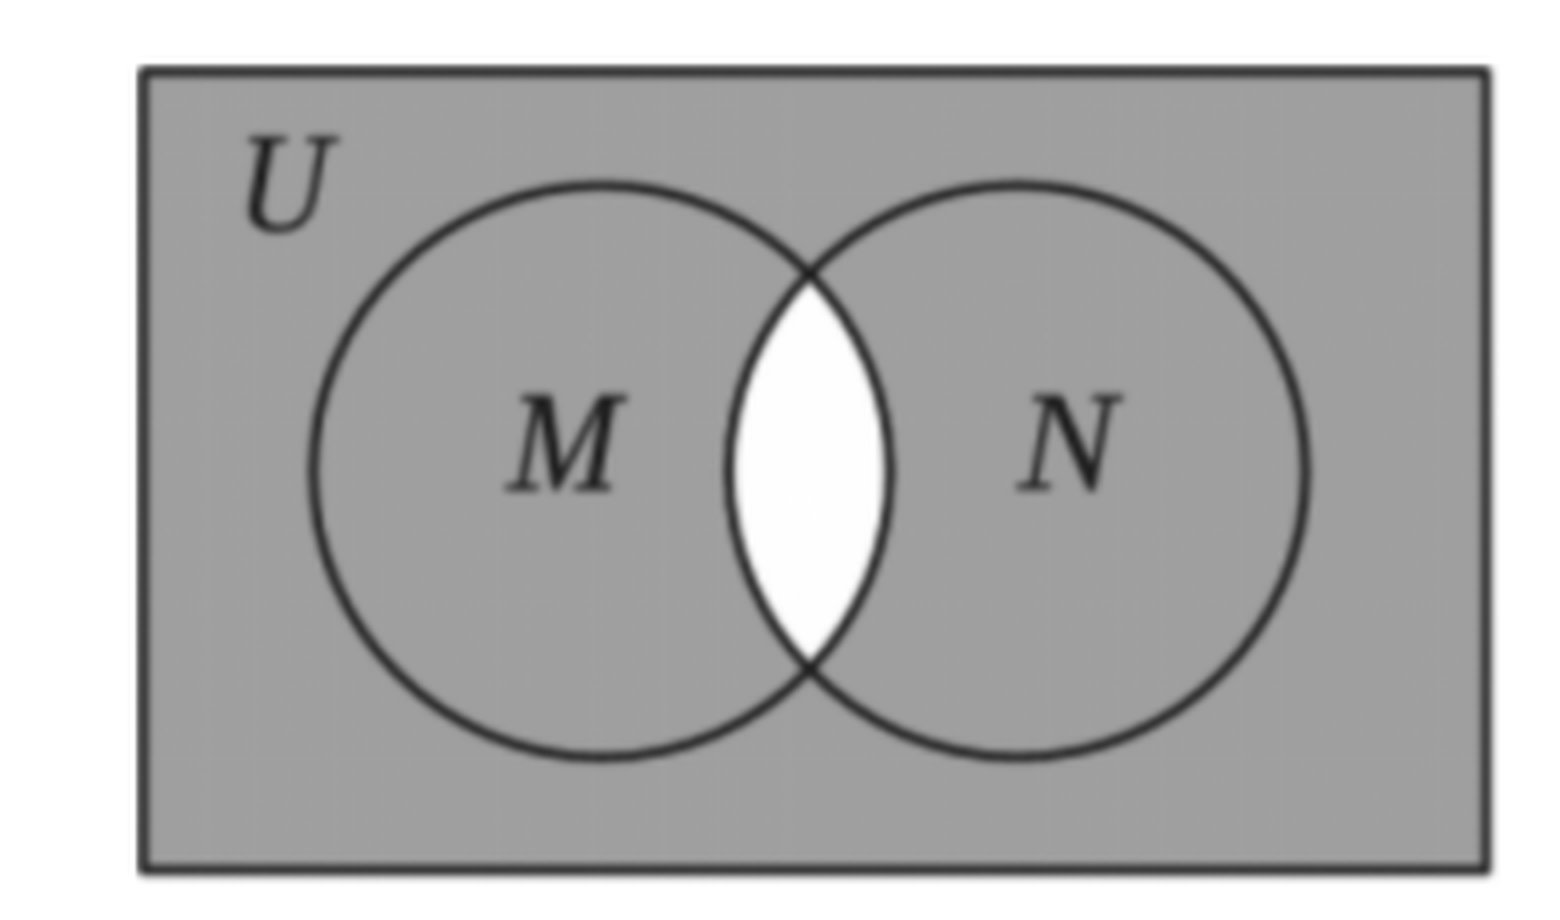
\includegraphics[width=0.40\textwidth]{figures/gao145_q14.png}
\end{center}

\ifanswer
\solbegin
\step{由韦恩图得图中白色区域为集合 $M\cap N$，所以阴影部分表示的集合为 $\overline{M\cap N}$.}
\step{故选 $D$.}
\solend
\fi

% === Q15 ===
\item 已知 $x>-2$，则 $x+\dfrac{1}{x+2}$ 的最小值为\mbox{（\quad）}

\keepwithprev
A. 3\qquad B. 2\qquad C. 1\qquad D. 0

\ifanswer
\solbegin
\step{$x>-2$，则 $x+2>0$，}
\step{所以 $x+\dfrac{1}{x+2}=(x+2)+\dfrac{1}{x+2}-2\geqslant2\sqrt{(x+2)\cdot\dfrac{1}{x+2}}-2=0$，}
\step{当且仅当 $x+2=\dfrac{1}{x+2}$，即 $x=-1$ 时取等号，所以 $x+\dfrac{1}{x+2}$ 的最小值为 $0$.}
\step{故选 $D$.}
\solend
\fi

% 第 16 题：题干在 05 页、解析续至 06 页；两幅数轴标根波浪曲线是【解析】内配图，
% 仅答案版出，放在答案版条件块内 \solbegin 的 \step 之间（照 高一73 第 16 题成例）
\item 关于 $x$ 的不等式 $\dfrac{(x-a)(x-2)^2}{(x-1)(x-5)}\leqslant0$ 的解集中恰有 3 个正整数，则实数 $a$ 的取值范围是\mbox{（\quad）}

\keepwithprev
A. $(-\infty,3]\cup[7,8)$\qquad B. $(-\infty,3)\cup[7,8)$\qquad C. $(-\infty,3]\cup(7,8]$\qquad D. $(-\infty,3)\cup(7,8]$

\ifanswer
\solbegin
\step{由题意，不等式 $\dfrac{(x-a)(x-2)^2}{(x-1)(x-5)}\leqslant0$，}
\step{可化为 $\begin{cases}(x-1)(x-2)^2(x-5)(x-a)\leqslant0\\x\ne1\text{且}x\ne5\end{cases}$，由数轴标根法，}
\step{当 $a=3$ 时，}
\begin{center}
% a=3 数轴标根图取 06 页，去粉色水印、去色、4× LANCZOS 放大；仅答案版出
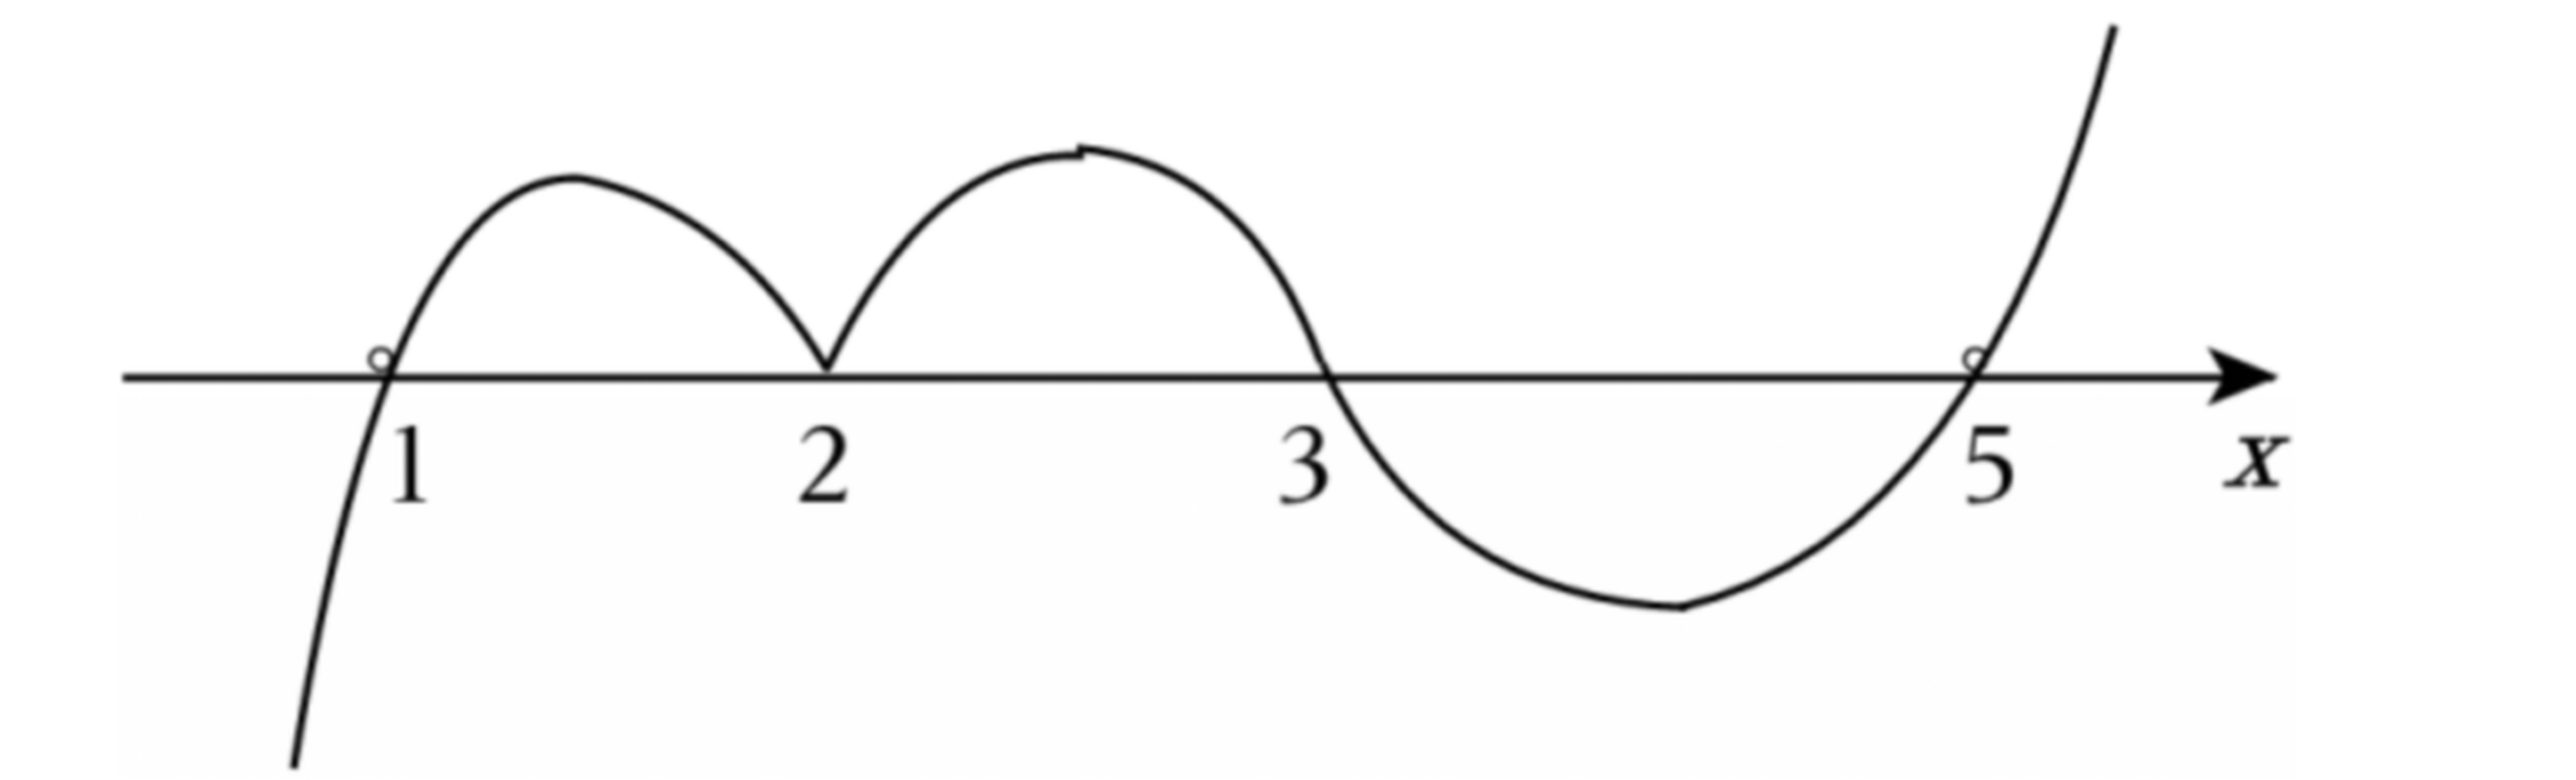
\includegraphics[width=0.62\textwidth]{figures/gao145_q16_a3.png}
\end{center}
\step{得不等式的解集为 $\{x\mid x<1\text{ 或 }x=2\text{ 或 }3\leqslant x<5\}$，}
\step{对应的正整数解为 $2$，$3$，$4$，满足题意，故排除 $B$、$D$；}
\step{当 $a=7$ 时，}
\begin{center}
% a=7 数轴标根图取 06 页，去粉色水印、去色、4× LANCZOS 放大；仅答案版出
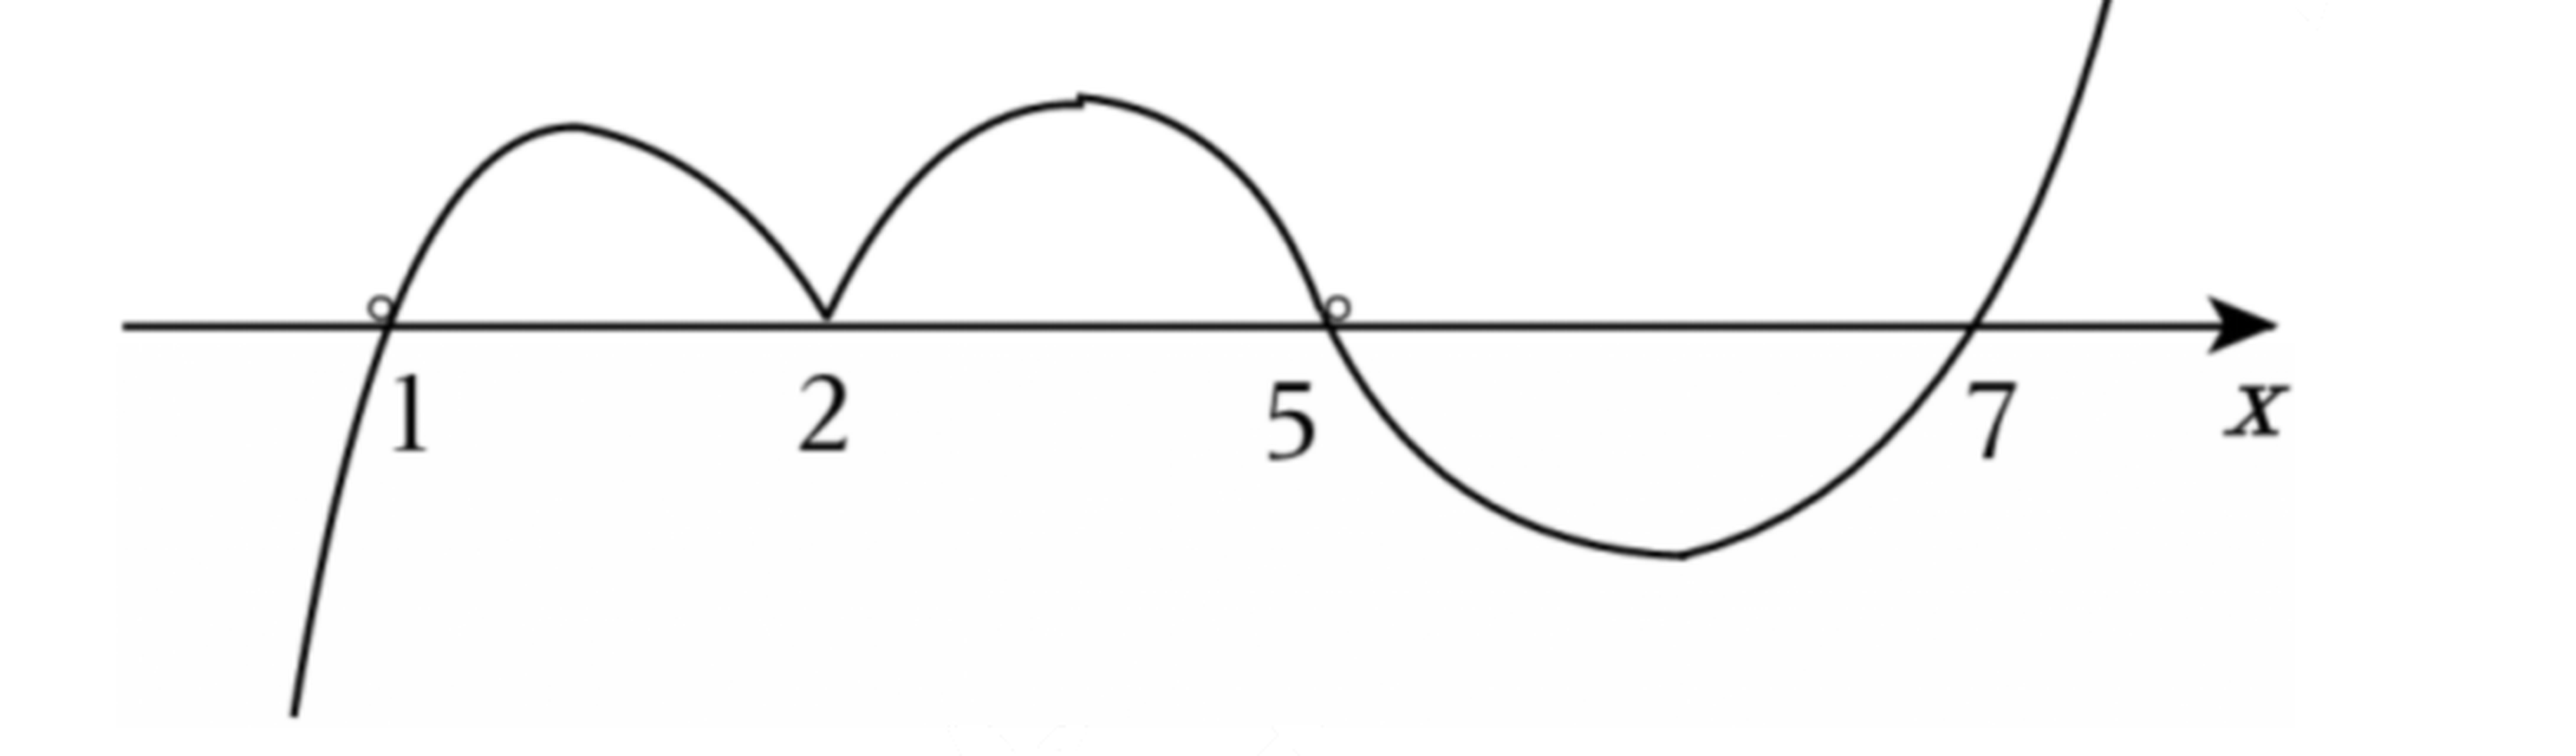
\includegraphics[width=0.62\textwidth]{figures/gao145_q16_a7.png}
\end{center}
\step{得不等式的解集为 $\{x\mid x<1\text{ 或 }x=2\text{ 或 }5<x\leqslant7\}$，}
\step{对应的正整数解为 $2$，$6$，$7$，满足题意，故 $A$ 正确，$C$ 错误.}
\step{故选 $A$.}
\solend
\fi

\end{enumerate}

\bigsec{三、解答题}

\begin{enumerate}
\setcounter{enumi}{16}

% 第 17 题：题干在 06 页、解析续至 07 页，按印刷行断，共 7 行；
% "lg(10÷5)" 的除号照录 \div
\item (1) 已知 $a+a^{-1}=6$，求 $a^2+a^{-2}$ 及 $a^{\frac12}-a^{-\frac12}$ 的值；

(2) 已知 $\lg5=a$，$\lg6=b$，用 $a$、$b$ 分别表示 $\lg2$、$\lg3$、$\lg300$ 和 $\log_{12}15$.

\ifanswer
\solbegin
\step{(1) 因为 $a+a^{-1}=6$，}
\step{所以 $a^2+a^{-2}=(a+a^{-1})^2-2\cdot a\cdot a^{-1}=6^2-2=34$，}
\step{因为 $\left(a^{\frac12}-a^{-\frac12}\right)^2=a-2+a^{-1}=6-2=4$，所以 $a^{\frac12}-a^{-\frac12}=\pm2$；}
\step{(2) $\lg2=\lg(10\div5)=\lg10-\lg5=1-a$，}
\step{$\lg3=\lg(6\div2)=\lg6-\lg2=b-(1-a)=a+b-1$，}
\step{$\lg300=\lg(3\times10^2)=\lg3+\lg10^2=a+b-1+2=a+b+1$，}
\step{所以 $\log_{12}15=\dfrac{\lg15}{\lg12}=\dfrac{\lg3+\lg5}{\lg3+\lg2^2}=\dfrac{a+b-1+a}{a+b-1+2(1-a)}=\dfrac{2a+b-1}{b-a+1}$.}
\solend
\fi

% 第 18 题：题干在 07 页、解析续至 08 页（2 问、分类讨论很长），按印刷行断共 25 行；
% 本卷 Q18 用"图像"（Q13/Q14 用"图象"），逐处照录不统一
\item 已知 $f(x)=(m^2-3m+1)x^{m^2-4m-1}$，$y=f(x)$ 为幂函数且在 $(0,+\infty)$ 上是严格减函数.

(1) 求实数 $m$ 的值以及相应的函数表达式；

(2) 若 $y=f(x)$ 的图像关于 $y$ 轴对称，解关于 $x$ 的不等式 $(x+2)^{1-m}<(3x-1)^{1-m}$.

\ifanswer
\solbegin
\step{(1) 由幂函数的定义得 $m^2-3m+1=1$，}
\step{整理得 $m^2-3m=0$，解得 $m=0$ 或 $m=3$，}
\step{由于 $y=f(x)$ 在 $(0,+\infty)$ 上为严格减函数，}
\step{因此幂函数的指数需满足 $m^2-4m-1<0$，}
\step{当 $m=3$ 时，指数为 $3^2-4\times3-1=-4<0$，满足严格递减条件，}
\step{此时函数表达式为 $f(x)=x^{-4}$，}
\step{当 $m=0$ 时，指数为 $0^2-4\times0-1=-1<0$，满足严格递减条件，}
\step{此时函数表达式为 $f(x)=x^{-1}$，}
\step{所以满足条件的实数 $m$ 为 $0$ 或 $3$，}
\step{对应的函数表达式分别为 $f(x)=x^{-1}$、$f(x)=x^{-4}$；}
\step{(2) 函数图像关于 $y$ 轴对称即函数为偶函数，}
\step{对于 $f(x)=x^{-1}=\dfrac1x$，定义域为 $(-\infty,0)\cup(0,+\infty)$，}
\step{满足 $f(-x)=-f(x)$，为奇函数，图像关于原点对称，}
\step{不满足关于 $y$ 轴对称的条件；}
\step{对于 $f(x)=x^{-4}=\dfrac{1}{x^4}$，定义域为 $(-\infty,0)\cup(0,+\infty)$，}
\step{满足 $f(-x)=f(x)$，为偶函数，图像关于 $y$ 轴对称，}
\step{因此符合条件的 $m$ 值为 $3$，}
\step{将 $m=3$ 代入关于 $x$ 的不等式 $(x+2)^{1-m}<(3x-1)^{1-m}$，}
\step{得 $(x+2)^{1-3}<(3x-1)^{1-3}$，即 $(x+2)^{-2}<(3x-1)^{-2}$，}
\step{因为负指数幂的底数不能为 $0$，所以 $x+2\ne0$ 且 $3x-1\ne0$，}
\step{即 $x\ne-2$ 且 $x\ne\dfrac13$，}
\step{不等式可变形为 $\dfrac{1}{(x+2)^2}<\dfrac{1}{(3x-1)^2}$，}
\step{整理得 $(3x-1)^2<(x+2)^2$，即 $8x^2-10x-3<0$，}
\step{解得 $-\dfrac14<x<\dfrac32$，又 $x\ne-2$ 且 $x\ne\dfrac13$，}
\step{所以不等式的解集为 $\left(-\dfrac14,\dfrac13\right)\cup\left(\dfrac13,\dfrac32\right)$.}
\solend
\fi

% 第 19 题：题干在 08 页、解析续至 09 页，按印刷行断，共 14 行；
% 判别式 cases 块内"△=4a²−16a<0"原卷印扁等边三角 \triangle
%（放大 09 页 zz09_delta.png 与 Q12 高 \Delta 并排确认），逐处照录不统一
\item 已知 $f(x)=ax^2+2ax+4$，$a\in\R$.

(1) 若关于 $x$ 的不等式 $f(x)>0$ 在实数集 $\R$ 上恒成立，求实数 $a$ 的取值范围；

(2) 当 $a<0$ 时，解关于 $x$ 的不等式 $f(x)>(a+1)x+5$.

\ifanswer
\solbegin
\step{(1) 由题意得，关于 $x$ 的不等式 $f(x)>0$ 在实数集 $\R$ 上恒成立，}
\step{即 $ax^2+2ax+4>0$ 在实数集 $\R$ 上恒成立，}
\step{当 $a=0$ 时，不等式为 $4>0$ 恒成立，符合题意；}
\step{当 $a\ne0$ 时，则 $\begin{cases}a>0\\\triangle=4a^2-16a<0\end{cases}$，解得 $0<a<4$.}% 判别式原卷印扁等边三角 $\triangle$，照录
\step{综上所述，实数 $a$ 的取值范围为 $[0,4)$.}
\step{(2) $f(x)=ax^2+2ax+4$，}
\step{当 $a<0$ 时，不等式 $f(x)>(a+1)x+5$ 即为 $ax^2+(a-1)x-1>0$，}
\step{即 $(ax-1)(x+1)>0$，即 $\left(x-\dfrac1a\right)(x+1)<0$，}
\step{当 $a<-1$，即 $\dfrac1a>-1$ 时，解得 $-1<x<\dfrac1a$；}
\step{当 $a=-1$，即 $\dfrac1a=-1$ 时，解得 $x\in\varnothing$；}
\step{当 $-1<a<0$，即 $\dfrac1a<-1$ 时，解得 $\dfrac1a<x<-1$.}
\step{综上所述，当 $a<-1$ 时，不等式的解集为 $\left\{x\mid -1<x<\dfrac1a\right\}$；}
\step{当 $a=-1$ 时，不等式的解集为 $\varnothing$；}
\step{当 $-1<a<0$ 时，不等式的解集为 $\left\{x\mid \dfrac1a<x<-1\right\}$.}
\solend
\fi

% 第 20 题：菜园靠墙图为题目配图（三版都出），题干写"如图"；
% 题干在 09 页（含图）、解析续至 10 页，按印刷行断，共 13 行
\needvspace{8cm}
\item 如图，某人计划用篱笆围成一个一边靠墙（墙足够长）的矩形菜园. 设菜园的长为 $x$ 米，宽为 $y$ 米.

\begin{center}
% 矩形菜园靠墙图取 09 页右下，去粉色水印、去色、4× LANCZOS 放大
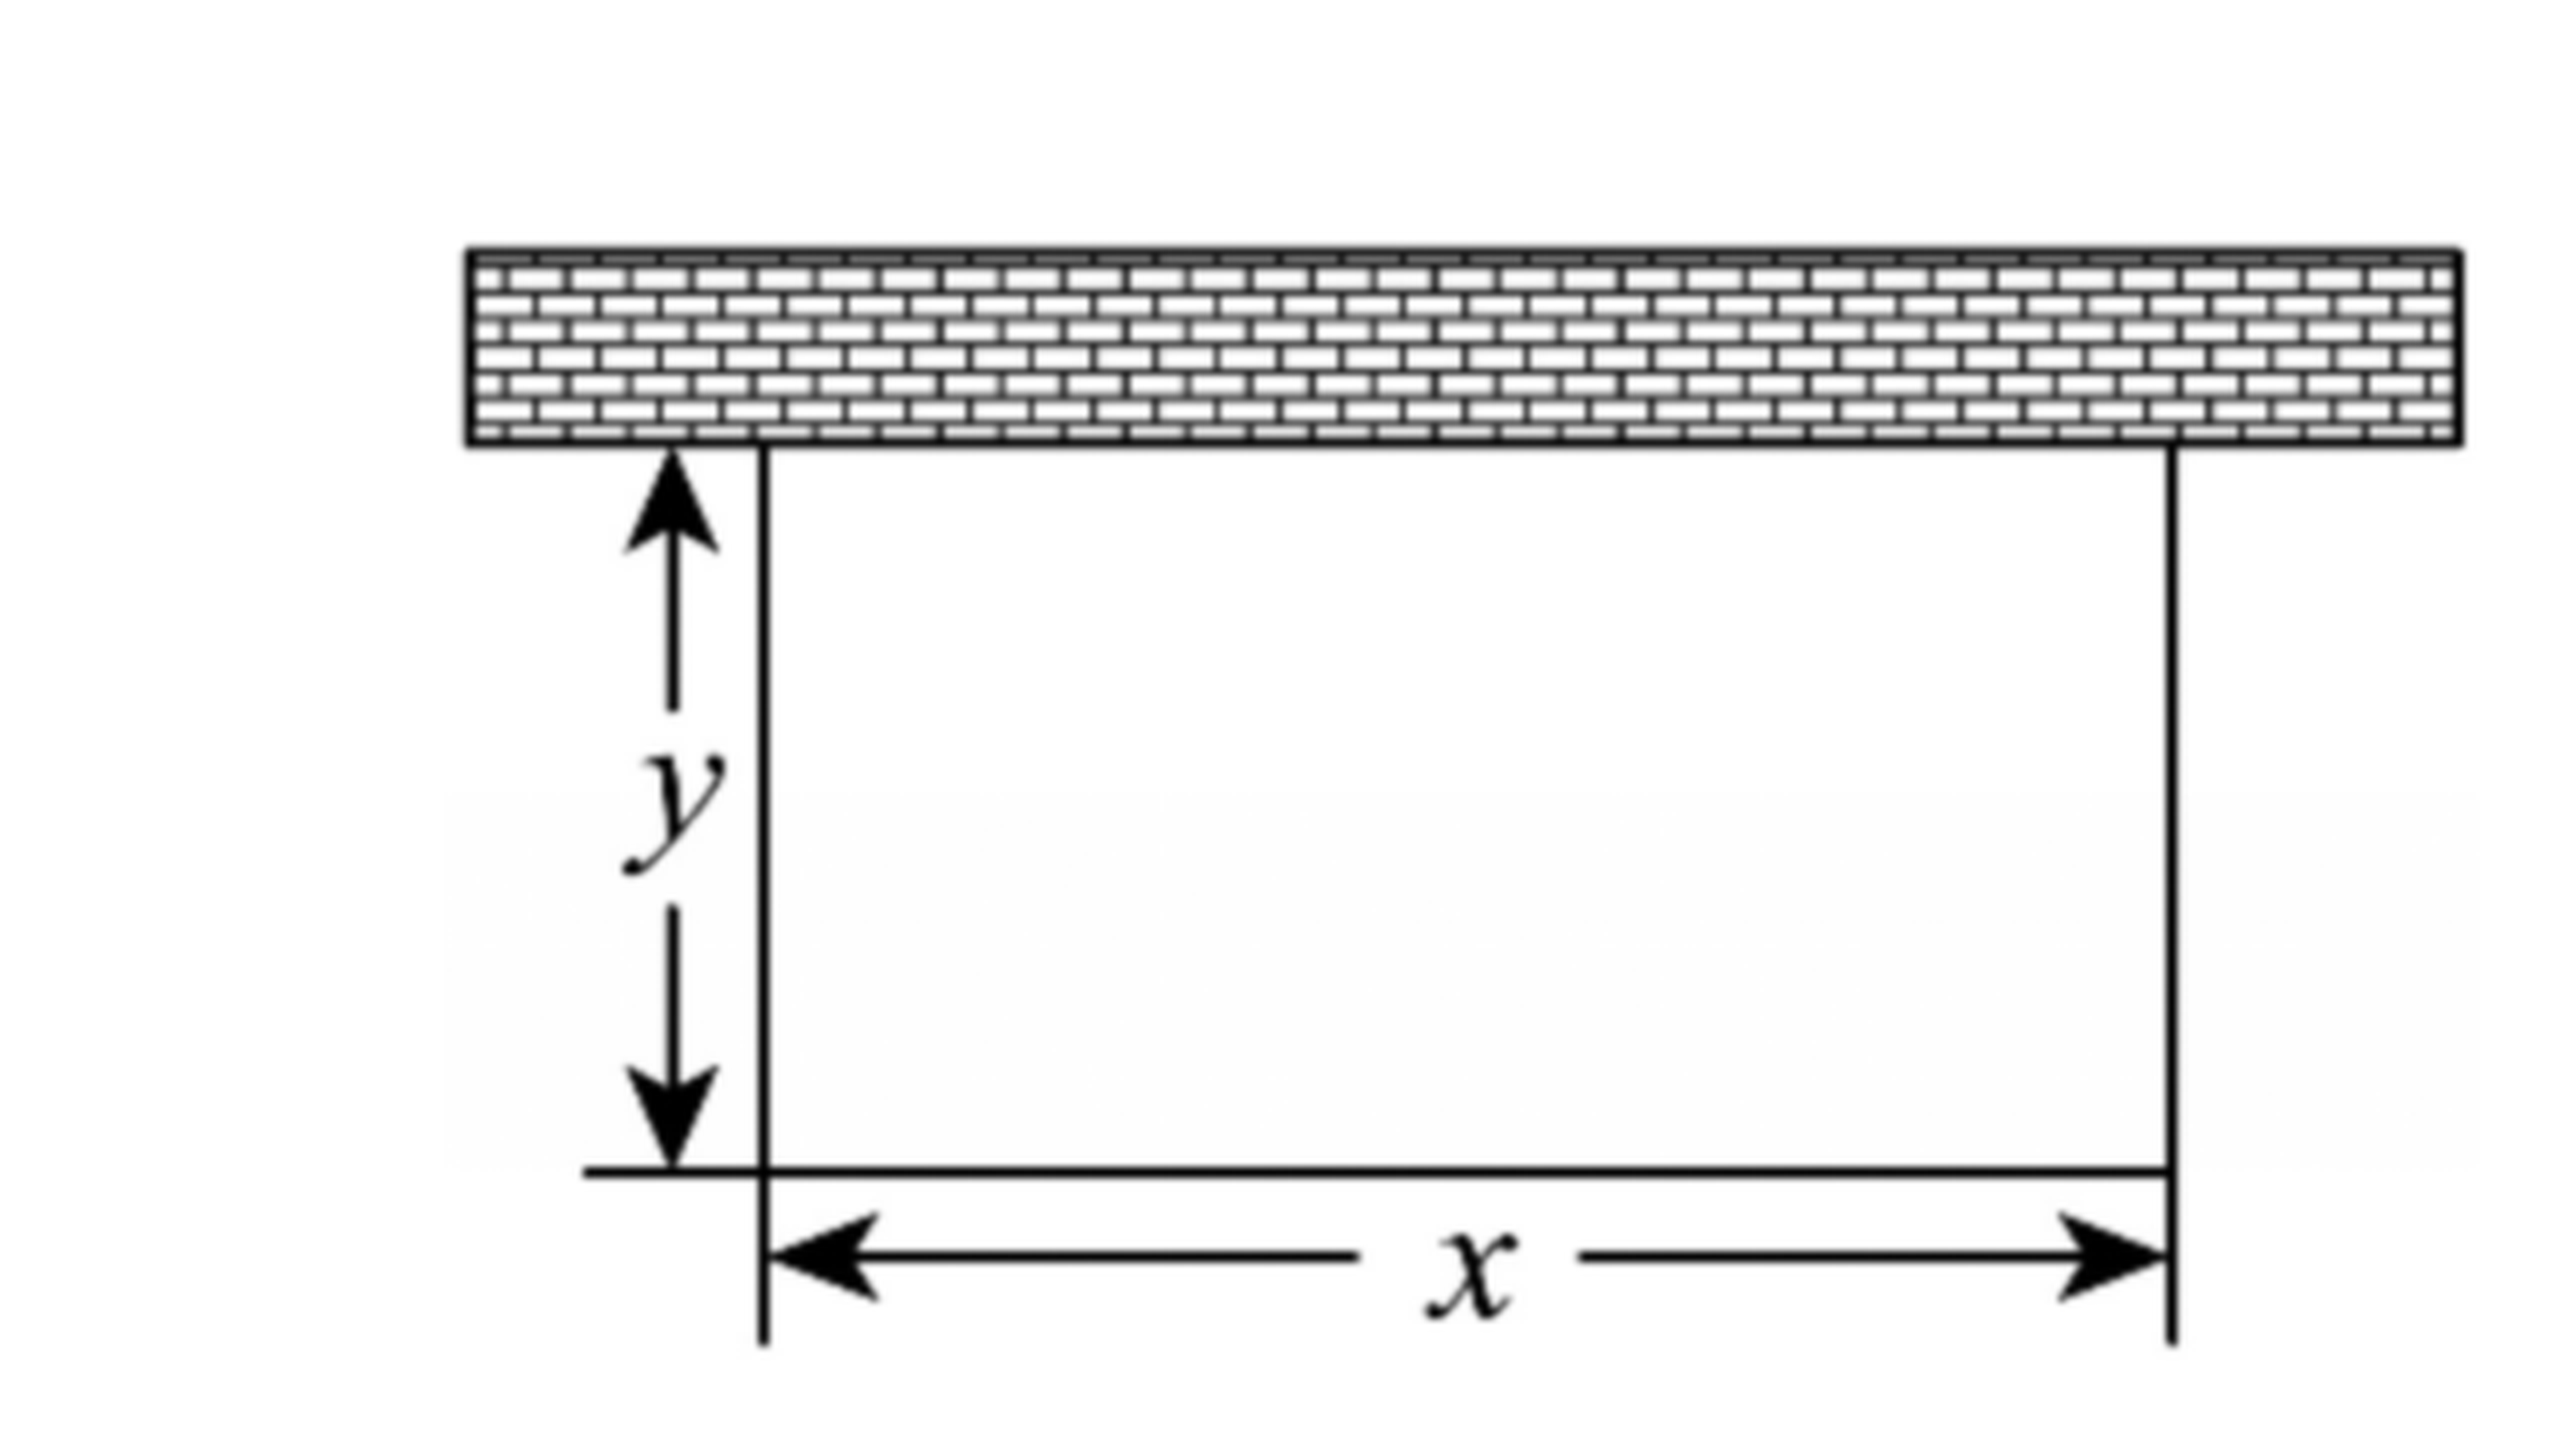
\includegraphics[width=0.55\textwidth]{figures/gao145_q20.png}
\end{center}

(1) 若菜园面积为 72 平方米，则 $x$、$y$ 为何值时，所用篱笆总长最小？

(2) 若 $x$、$y$ 满足 $x+y-xy+63=0$，则菜园面积最小为多少平方米？

\ifanswer
\solbegin
\step{(1) 由题意得，菜园的面积 $S=xy=72$，且 $x>0$，$y>0$，}
\step{所用篱笆总长 $L=x+2y$，}
\step{由基本不等式得 $x+2y\geqslant2\sqrt{x\cdot2y}=2\sqrt{2xy}=2\sqrt{2\times72}=24$，}
\step{当且仅当 $x=2y$ 时取等号，}
\step{联立 $\begin{cases}xy=72\\x=2y\end{cases}$，解得 $\begin{cases}x=12\\y=6\end{cases}$，}
\step{所以当 $x=12$，$y=6$ 时，所用篱笆总长最小；}
\step{(2) 由题意得 $x>0$，$y>0$，且满足 $x+y-xy+63=0$，即 $x+y=xy-63$，}
\step{由基本不等式得 $x+y\geqslant2\sqrt{xy}$，当且仅当 $x=y$ 时取等号，}
\step{所以 $xy-63\geqslant2\sqrt{xy}$. 令 $t=\sqrt{xy}(t>0)$，则 $xy=t^2$，}
\step{上述不等式可化为 $t^2-2t-63\geqslant0$，即 $(t-9)(t+7)\geqslant0$，}
\step{因为 $t>0$，所以 $t+7>0$，故 $t-9\geqslant0$，解得 $t\geqslant9$，所以 $\sqrt{xy}\geqslant9$，}
\step{即 $xy\geqslant81$，当且仅当 $x=y=9$ 时取等号，此时满足 $9+9-81+63=0$，}
\step{所以菜园面积最小为 81 平方米.}
\solend
\fi

% 第 21 题：题干在 10 页、解析续至 11 页（3 问、分类讨论很长），按印刷行断共 22 行；
% 末行"故第 2026 个元素是 2700 之后第一个属于 A 的数，即 2701." 为全卷收尾，
% 无 Q22/Q23、无附加题节；数集 Z/N* 按全稿惯例改 \Z/\N^*
\item 已知集合 $A=\{x\mid x=m^2-n^2$，$m$、$n\in\Z\}$.

(1) 求证：任何奇数 $2k+1(k\in\Z)$ 都是集合 $A$ 中的元素；

(2) 判断偶数 $4k-2(k\in\Z)$ 是否为集合 $A$ 的元素？请说明理由；

(3) 若将集合 $A$ 中的正整数由小到大排列，求出集合 $A$ 中第 2026 个正整数.

\ifanswer
\solbegin
\step{(1) 因为 $x=(k+1)^2-k^2=2k+1(k\in\Z)$，}
\step{所以任何奇数 $2k+1(k\in\Z)$ 都属于集合 $A$；}
\step{(2) 偶数 $4k-2(k\in\Z)$ 不是集合 $A$ 的元素，理由如下：}
\step{由题意得 $x=m^2-n^2=(m-n)(m+n)$，}
\step{当 $m$、$n$ 均为奇数时，设 $m=2k_1+1$，$n=2k_2+1(k_1$、$k_2\in\Z)$，}
\step{则 $m^2-n^2=(2k_1+1)^2-(2k_2+1)^2=(2k_1-2k_2)(2k_1+2k_2+2)$}
\step{$=4(k_1-k_2)(k_1+k_2+1)$，}
\step{因为 $k_1$、$k_2\in\Z$，所以 $k_1-k_2\in\Z$，$k_1+k_2+1\in\Z$，}
\step{从而 $m^2-n^2$ 为 $4$ 的倍数；}
\step{当 $m$、$n$ 均为偶数时，设 $m=2k_1$，$n=2k_2(k_1$、$k_2\in\Z)$，}
\step{$m^2-n^2=4k_1^2-4k_2^2=4(k_1^2-k_2^2)$ 为 $4$ 的倍数；}
\step{当 $m$、$n$ 为一个偶数一个奇数时，不妨设 $m$ 为偶数，$n$ 为奇数，}
\step{设 $m=2k_1$，$n=2k_2+1(k_1$、$k_2\in\Z)$，}
\step{则 $m^2-n^2=4k_1^2-(2k_2+1)^2=4(k_1^2-k_2^2-k_2)-1$ 为奇数.}
\step{无论哪种情况均不满足 $4k-2(k\in\Z)$，}
\step{故偶数 $4k-2(k\in\Z)$ 不是集合 $A$ 的元素；}
\step{(3) 由前两问得，$4$ 的倍数和奇数属于集合 $A$ 中的元素，}
\step{令集合 $A$ 中的正整数元素为 $4k-3$、$4k-1$、$4k(k\in\N^*)$，}
\step{对任意的 $k\in\N^*$，连续的 $4$ 个整数 $4k-3$、$4k-2$、$4k-1$、$4k$ 中}
\step{有三个数 $4k-3$、$4k-1$、$4k$ 都在集合 $A$ 中，}
\step{因为 $2026=3\times675+1$，所以集合 $A$ 中第 $2025$ 个元素为 $4\times675=2700$，}
\step{故第 2026 个元素是 2700 之后第一个属于 $A$ 的数，即 2701.}
\solend
\fi

\end{enumerate}

\end{document}
"
% 紧凑版：xelatex "\def\iscompact{1}% 高一145_市二中学_期中.tex
%   —— 高一上数学"2026-2027 年市二中学高一上期中"（试卷版/答案版/紧凑版）
% 试卷版：xelatex 高一145_市二中学_期中.tex
% 答案版：xelatex "\def\isanswer{1}\input{高一145_市二中学_期中.tex}"
% 紧凑版：xelatex "\def\iscompact{1}\input{高一145_市二中学_期中.tex}"
%
% ① 原始材料：微信公众号"魔都数学加油站"文章，连载"27学年高一145"，原文标题
% "27学年高一145——2026-2027年上海市市二中学高一上期中"；
% 原文链接：https://mp.weixin.qq.com/s/6V-i9KE0GWodC-wmd5z8nQ 。
% 正文为 11 张 PNG 页（01/02/03/08/10/11 为 4762×6735，04/05/06/07/09 为 2560×3620，
% 同一篇各页分辨率不同，逐页按各自分辨率裁图核对，别按预览比例换算裁框）。
% 题目下印【答案】或【解析】，为混合体例讲评版：Q3 只印【答案】、无【解析】，其余
% 18 题印【解析】。题目、解析均据原图转录；卷面粉红色水印"魔都数学加油站"及
% 公众号页脚未录入。
% 全卷插图情况（逐页通读 11 页确认，题干写"如图"处均配有图）：
%   · Q14 韦恩图（05 页右侧，全集 U 矩形＋两圆 M/N＋白色交集、灰色阴影＋U/M/N 标注）：
%     题目配图（选择题选项旁），三版都出，裁自 05 页去水印去色 4× 放大存
%     figures/gao145_q14.png；
%   · Q16 两幅数轴标根波浪曲线（06 页，a=3 与 a=7 各一幅，标根法画
%     (x-1)(x-2)^2(x-5)(x-a)≤0 的符号曲线）：【解析】内的配图，仅答案版出，
%     裁 figures/gao145_q16_a3.png / figures/gao145_q16_a7.png（或合并一张），
%     放在答案版条件块内 \solbegin 的 \step 之间（照 高一73 第 16 题成例）；
%   · Q20 矩形菜园靠墙图（09 页右下，灰色砖墙＋矩形菜园＋x/y 标注＋箭头）：
%     题目配图，三版都出，裁自 09 页去水印去色 4× 放大存 figures/gao145_q20.png；
%   其余各页逐页确认无其它题目配图、无表格、亦无"题干写如图而源码漏图"一处。
%
% 卷首标题：原卷印作"2026-2027 年市二中学高一上期中"，年份区间按全稿惯例排 en dash；
% 原卷卷面未印副标题，本稿按同期中卷（高一140／141／143／144）知识模块口径补出
% "集合与常用逻辑用语、不等式、函数"。
%
% 题号体例：本卷共 19 题——一、填空题 3—12（10 题）、二、选择题 13—16（4 题）、
% 三、解答题 17—21（5 题）。三节分别 \setcounter{enumi}{2}／{12}／{16}。
% 原卷从第 3 题起、无第 1、2 题，本稿保留原题号；全卷无附加题节。
%
% ② 与原卷的排版差异：
%   ① 原文从第 3 题起，本稿保留原题号；共 19 题三节；
%   ② 混合体例：原卷 Q3 只印【答案】、无【解析】（"第一步应假设___。
%      【答案】x≤2 或 y≤2"），按 高一140 第 5 题成例提 \ans{}、不补造解析；
%      其余 18 题印【解析】，用 \solbegin…\solend，选择题答案在解析末句"故选 X"
%      （Q13 选 B、Q14 选 D、Q15 选 D、Q16 选 A，逐个放大原图核实）、
%      题干括号 \mbox{（\quad）} 留空、不另提 \ans{}；填空／解答答案落在解析里；
%      答案版【答案】/【解析】标记数 = 19（1 个 \ans ＋ 18 个 \solbegin）= 全卷题数；
%   ③ 原卷卷面未印副标题，本稿按知识模块口径补出；
%   ④ 原卷填空横线按全稿惯例排 \blankline[4.4em]；选择题括号排 \mbox{（\quad）}、
%      选项段前按惯例加 \keepwithprev；解答题不留作答区、不加 \anspace
%      （原卷为讲评版，与 129／131／132／133／136／140／141／143／144 同）；
%   ⑤ 数集：Q9"a、b∈R"、Q12"a∈R"、Q21"m、n∈Z""k∈Z""k∈N*"等原卷印
%      斜体或黑板粗体 R/Z/N，按全稿惯例统一改 \R／\Z／\N^*；绝对值排 \lvert…\rvert，
%      集合描述竖线排 \mid；不等号按全稿惯例排 \leqslant／\geqslant；
%      补集照原卷上划线排 \overline{M}／\overline{N}（Q14 选项 B/C/D 逐处核）；
%      空集记号 \varnothing；\subset（单线⊂）与 \subseteq（带下划线⊆）逐处照录不统一；
%   ⑥ 子题标号 (1)(2)(3) 原卷印半角括号照录；圈数字进数学式用 \text{①}（否则 FONTCHK 挂）；
%      \left…\right 不得拆到不同 $…$ 组；cases 块整体算一个印刷行；
%   ⑦ 题干／解析中的中文弯引号按原卷照录（Q3"若 x+y>4，则 x>2 且 y>2"、
%      Q11"a₁/a₂=b₁/b₂""M=N"、选填"充分非必要""必要非充分""充要""既非充分也非必要"
%      等，含引号内空格），注释内一律 ASCII 引号；数学式内 CJK 用 \text{}；
%   ⑧ 半角逗号在数学组之间是全稿惯例、非笔误（如 Q5"x₁+x₂=6，x₁x₂=√3"、
%      Q7"a>1，b>1"、指数／对数式内逗号），逐处照录别改全角；行末西文句点照录为
%      ASCII `.`；行中全角逗号／顿号照录；
%   ⑨ "图像／图象"逐处照录不统一（Q18"图像关于 y 轴对称"等，核全卷）；
%   ⑩ 判别式 Δ/△ 混用是照录项：Q12 解析"Δ=a²−4a²(2a−3)>0"、
%      Q19 解析"Δ=4a²−16a<0"等，放大原图判断是高 \Delta（等腰偏高、高>宽）
%      还是扁 \triangle，逐处照录不得统一（参照 高一142／144 头注④口径）；
%   ⑪ 一条 \step = 原卷解析的一个印刷行，cases 块整体算一个印刷行；别把原卷折行
%      并起来、别把一行拆多条。Q6 分段讨论、Q12 三个 cases 条件组、Q16 数轴标根、
%      Q18／Q19 分类讨论、Q21 三问均按印刷行逐条断，不丢行；
%   ⑫ Q14 韦恩图为"题干＋选项＋图"整块，加 \needvspace 守卫推走（守卫放 \item 之前，
%      见 高一140 Q14、高一144 Q17 成例与切页审计 B 类坑）；Q20 菜园图同理；
%      三版切页审计均"合计异常：无"；
%   ⑬ 跨页续印按题合并：Q3/4/5/6 在 01 页（Q6 解析续 02 页顶）；Q7/8/9/10 在 02 页
%      （Q10 解析续 03 页）；Q11/12 在 03 页（Q12 解析续 04 页，很长）；
%      Q13 在 04 页末、解析在 05 页顶；Q14/15/16 在 05 页（Q16 解析续 06 页含两幅数轴图）；
%      Q17 在 06 页、解析续 07 页；Q18 在 07 页、解析续 08 页；Q19 在 08 页、解析续 09 页；
%      Q20 在 09 页（含菜园图）、解析续 10 页；Q21 在 10 页、解析续 11 页
%      （末页收尾"故第 2026 个元素是 2700 之后第一个属于 A 的数，即 2701."、
%      无 Q22/Q23、无附加题节）。本稿按题连排，不丢行、不并折行；
%   ⑭ 原卷解析内若有红色"法一／法二"之类小标题，按全稿惯例排 \stepm{标签}{…}
%      （黑体着色、不引入红色、不改 common.sty），头注注明；水印"魔都数学加油站"
%      红色不录入。
%
% ③ 行数复核：一条 \step／\stepm = 原卷解析的一个印刷行，cases 块作一个印刷行计。
%   逐题数（主会话逐页核对定稿）：Q3：0（只印【答案】、提 \ans{}，不计入 \step 账）；
%   Q4：3；Q5：2；Q6：10；Q7：3；Q8：3；Q9：2；Q10：7；Q11：4；Q12：12；
%   Q13：2；Q14：2；Q15：4；Q16：9；Q17：7；Q18：25；Q19：14；Q20：13；Q21：22。
%   合计 144 条 \step（本卷无 \stepm：解析内无红色"法一／法二"类小标题），
%   与原卷逐题印刷行相等。全卷 18 题设 \solbegin…\solend ＋ Q3 一处 \ans{}，
%   答案版【答案】/【解析】标记数 = 19 = 全卷题数。
%
% ④ 判别式／子集符号结论（逐处放大原图照录、不得统一，主会话像素级复核）：
%   判别式全卷 2 处、两形混用逐处照录不统一（参照 高一142／144 头注④口径）：
%     · Q12 解析 cases 块"Δ=a²−4a²(2a−3)>0" 原卷印等腰偏高粗三角（高>宽），
%       照录 \Delta（放大 04 页 /tmp/gao145s2/main_q12_delta.png 确认）；
%     · Q19 解析 cases 块"△=4a²−16a<0" 原卷印扁等边空心三角（宽≈高、细线），
%       照录 \triangle（放大 09 页 /tmp/gao145s2/main_q19_delta.png 确认）。
%   子集／补集：Q14 选项 A `M\cup N`、B `M\cap\overline{N}`（上划线只在 N 上）、
%   C `\overline{M\cup N}`（罩整个 M∪N）、D `\overline{M\cap N}`（罩整个 M∩N，
%   非 \overline{M}\cap N；放大 05 页 /tmp/gao145s2/main_q14_opts.png 确认），
%   阴影为灰色区域＝全集减白色交集，答案 D，照录 \overline{M\cap N}；
%   全集卷无 \subset／\subseteq 混用（本卷集合题用 \cup／\cap／\overline{}）；
%   空集 \varnothing（Q19 解析 x∈\varnothing）；数集 \R／\Z／\N^* 归一见 ② ⑤。
%
% ⑤ 存疑照录（放大原图确认，照录未改、正文对应处另有 % 注）：
%   1. Q3 题干"若 x+y>4，则 x>2 且 y>2" 后"时"前留一空格、弯引号内空格照录；
%      该卷混合体例（Q3 只印【答案】、提 \ans{}）见 ② ②。
%   2. Q4／Q5 解析中的"1，3，5 和 6"、"x₁+x₂=6,x₁x₂=√3" 等半角／全角逗号
%      逐处照原卷（放大 01 页确认），数学式内半角逗号为全稿惯例、非笔误。
%   3. Q14 选项 D 上划线罩住整个 M∩N（而非仅罩 M），照录 \overline{M\cap N}。
%   4. Q12 判别式高 \Delta 与 Q19 判别式扁 \triangle 两形混用，逐处照录不统一（见 ④）。
%   全卷除此 4 类外未发现其它笔误／自相矛盾处。
%
% ⑥ 跨页续印按题合并说明：见 ② ⑬。
%
\documentclass[a4paper,11pt]{article}
\usepackage{common}

\begin{document}

\examtitlest[3]{2026--2027 年市二中学高一上期中}{集合与常用逻辑用语、不等式、函数}

\bigsec{一、填空题}

\begin{enumerate}
\setcounter{enumi}{2}

% 第 3 题：原卷只印【答案】、无【解析】（放大 01 页确认），按 高一140 第 5 题成例
% 提 \ans{}、不补造解析；题干中文弯引号与"时"前空格照录
\item 用反证法证明命题：“若 $x+y>4$，则 $x>2$ 且 $y>2$” 时，第一步应假设\blankline[4.4em].

\ifanswer
\ans{$x\leqslant2$ 或 $y\leqslant2$}
\fi

% === Q4 ===
\item 设集合 $M$ 满足 $\{1,3,5,6\}\cup M=\{1,2,3,4,5,6\}$，则满足条件的所有 $M$ 的个数为\blankline[4.4em].

\ifanswer
\solbegin
\step{集合 $M$ 满足 $\{1,3,5,6\}\cup M=\{1,2,3,4,5,6\}$，}
\step{则 $M$ 中必含有 $2$ 和 $4$，$1$，$3$，$5$ 和 $6$ 可以选也可不选，}
\step{则满足条件的所有 $M$ 的数目相当于集合 $\{1,3,5,6\}$ 的子集的个数 $2^4=16$.}
\solend
\fi

% === Q5 ===
\item 已知方程 $x^2-6x+\sqrt3=0$ 的两根为 $x_1$ 和 $x_2$，则 $(x_1-x_2)^2=$\blankline[4.4em].

\ifanswer
\solbegin
\step{因为方程 $x^2-6x+\sqrt3=0$ 的两根为 $x_1$ 和 $x_2$，所以 $x_1+x_2=6,x_1x_2=\sqrt3$，}% 数学式内半角逗号为全稿惯例，照录
\step{所以 $(x_1-x_2)^2=(x_1+x_2)^2-4x_1x_2=36-4\sqrt3$.}
\solend
\fi

% 第 6 题：题干在 01 页，解析续至 02 页顶（末 2 行），按印刷行逐条断，共 10 行
\item 不等式 $\lvert x-2026\rvert+\lvert x-2029\rvert>3$ 的解集是\blankline[4.4em].

\ifanswer
\solbegin
\step{当 $x<2026$ 时，$x-2026<0$，$x-2029<0$，}
\step{原不等式可化为 $(2026-x)+(2029-x)>3$，解得 $x<2026$，}
\step{故此时，不等式的解为 $x<2026$；}
\step{当 $2026\leqslant x\leqslant2029$ 时，$x-2026\geqslant0$，$x-2029\leqslant0$，}
\step{原不等式可化为 $(x-2026)+(2029-x)>3$，即 $3>3$，显然不成立，}
\step{故此时，不等式无解；}
\step{当 $x>2029$ 时，$x-2026>0$，$x-2029>0$，}
\step{原不等式可化为 $(x-2026)+(x-2029)>3$，解得 $x>2029$，}
\step{故此时，不等式的解为 $x>2029$.}
\step{综上，原不等式的解集为 $(-\infty,2026)\cup(2029,+\infty)$.}
\solend
\fi

% === Q7 ===
\item 已知 $a>1$，$b>1$，若 $\log_a b+\log_b a=2$，且 $ab=2$，则 $\log_2(a+b)=$\blankline[4.4em].

\ifanswer
\solbegin
\step{由 $\log_a b+\log_b a=2$，$a>1$，$b>1$，得 $\log_a b+\dfrac{1}{\log_a b}=2$，}
\step{即 $(\log_a b)^2-2\log_a b+1=0$，则 $(\log_a b-1)^2=0$，解得 $\log_a b=1$，即 $a=b$，}
\step{又 $ab=2$，所以 $a=b=\sqrt2$，所以 $\log_2(a+b)=\log_2 2\sqrt2=\log_2 2^{\frac32}=\dfrac32$.}
\solend
\fi

% === Q8 ===
\item 已知 $m>0$，$n>0$，且 $m+n=1$，则 $\dfrac1m+\dfrac4n$ 的最小值为\blankline[4.4em].

\ifanswer
\solbegin
\step{由 $m>0$，$n>0$，$m+n=1$，}
\step{则 $\dfrac1m+\dfrac4n=(m+n)\left(\dfrac1m+\dfrac4n\right)=5+\dfrac nm+\dfrac{4m}n\geqslant5+2\sqrt{\dfrac nm\cdot\dfrac{4m}n}=9$，}
\step{当且仅当 $n=2m=\dfrac23$ 时，上式取得等号，故最小值为 $9$.}
\solend
\fi

% === Q9 ===
\item 已知 $a$、$b\in\R$，且 $3a+2b=1$，则 $8^a+4^b$ 最小值为\blankline[4.4em].

\ifanswer
\solbegin
\step{因为 $3a+2b=1$，所以 $8^a+4^b=2^{3a}+2^{2b}\geqslant2\sqrt{2^{3a+2b}}=2\sqrt2$，}
\step{当且仅当 $3a=2b$ 时取等号，故最小值为 $2\sqrt2$.}
\solend
\fi

% 第 10 题：题干在 02 页、解析续至 03 页顶，按印刷行断，共 7 行
\item 已知关于 $x$ 的不等式 $ax^2+bx+c>0$ 的解集为 $\{x\mid 1<x<2\}$，则关于 $x$ 的不等式 $bx^2-ax+c<0$ 的解集为\blankline[4.4em].

\ifanswer
\solbegin
\step{已知关于 $x$ 的不等式 $ax^2+bx+c>0$ 的解集为 $\{x\mid 1<x<2\}$，}
\step{由解集为 $1<x<2$ 且二次函数在两根之间为正，得 $a<0$，两个根为 $1$，$2$，}
\step{所以 $ax^2+bx+c=a(x-1)(x-2)=ax^2-3ax+2a$，}
\step{比较系数得 $b=-3a$，$c=2a$.}
\step{于是 $bx^2-ax+c=-3ax^2-ax+2a=-a(3x-2)(x+1)$，}
\step{$a<0$，故 $bx^2-ax+c<0$ 等价于 $(3x-2)(x+1)<0$，解得 $-1<x<\dfrac23$，}
\step{故 $bx^2-ax+c<0$ 的解集为 $\left\{x\mid -1<x<\dfrac23\right\}$.}
\solend
\fi

% 第 11 题：题干引号内空格照录（放大 03 页确认），四组选填引号亦同；
% 结论"故为必要非充分条件"照录，解析共 4 个印刷行
\item 设 $a_1$、$b_1$、$a_2$、$b_2$ 均为非零实数，不等式 $a_1x+b_1>0$ 和 $a_2x+b_2>0$ 的解集分别为集合 $M$、$N$，那么 “ $\dfrac{a_1}{a_2}=\dfrac{b_1}{b_2}$ ” 是 “ $M=N$ ” 的\blankline[4.4em]条件（选填 “ 充分非必要 ”、“ 必要非充分 ”、“ 充要 ” 和 “ 既非充分也非必要 ”）.

\ifanswer
\solbegin
\step{当 $a_1=b_1=1$，$a_2=b_2=-1$ 时，满足 $\dfrac{a_1}{a_2}=\dfrac{b_1}{b_2}$，}
\step{但是 $M=N$ 不成立，即充分性不成立；}
\step{若 $M=N$ 时，$\dfrac{a_1}{a_2}=\dfrac{b_1}{b_2}$ 一定成立，即必要性成立.}
\step{故为必要非充分条件.}
\solend
\fi

% 第 12 题：题干在 03 页、解析续至 04 页（很长，含 3 个 cases 条件组），
% 按印刷行逐条断共 12 行；cases 块整体算一个印刷行
\item 已知 $f(x)=\dfrac{ax+3}{x-2}$（常数 $a\in\R$）. 函数 $y=f(x)$ 在区间 $[3,+\infty)$ 上是严格减函数，且函数值不恒为负. 若关于 $x$ 的方程 $f(x)=\dfrac{a}{ax-1}$ 有两个不相等的实数根 $x_1$ 和 $x_2$，则 $a$ 的取值范围是\blankline[4.4em].

\ifanswer
\solbegin
\step{$f(x)=\dfrac{ax+3}{x-2}=a+\dfrac{3+2a}{x-2}$，定义域 $(-\infty,2)\cup(2,+\infty)$，}
\step{由于 $y=f(x)$ 在区间 $[3,+\infty)$ 上是严格减函数，且函数值不恒为负，}
\step{所以 $\begin{cases}3+2a>0\\a+\dfrac{3+2a}{3-2}\geqslant0\end{cases}\Rightarrow a\geqslant-1$，}
\step{若关于 $x$ 的方程 $f(x)=\dfrac{a}{ax-1}$ 有两个不相等的实数根 $x_1$ 和 $x_2$，}
\step{则 $\dfrac{ax+3}{x-2}=\dfrac{a}{ax-1}$，即 $(ax+3)(ax-1)=a(x-2)$，$x\ne2$ 且 $ax-1\ne0$，}
\step{当 $a\ne0$ 且 $a\geqslant-1$ 时，$(ax+3)(ax-1)=a(x-2)$，$x\ne2$ 且 $ax-1\ne0$，}
\step{可化为 $\begin{cases}a^2x^2+ax+2a-3=0\\x\ne2,x\ne\dfrac1a\end{cases}$，}
\step{要使方程有两个不相等的实数根 $x_1$ 和 $x_2$，}
\step{则 $\begin{cases}\Delta=a^2-4a^2(2a-3)>0\\a\geqslant-1\text{且}a\ne0\\4a^2+2a+2a-3\ne0\\a^2\cdot\dfrac1{a^2}+a\cdot\dfrac1a+2a-3\ne0\end{cases}\Rightarrow\begin{cases}a<\dfrac{13}{8}\\a\geqslant-1\text{且}a\ne0\\a\ne\dfrac12\text{且}a\ne-\dfrac32\\a\ne\dfrac12\end{cases}$，}% 判别式原卷印等腰偏高三角 $\Delta$，照录（放大 04 页 zz04_delta.png 确认）
\step{得 $-1\leqslant a<\dfrac{13}{8}$ 且 $a\ne0,a\ne\dfrac12$；}
\step{当 $a=0$ 时，方程无解；}
\step{所以 $a$ 的取值范围是 $[-1,0)\cup\left(0,\dfrac12\right)\cup\left(\dfrac12,\dfrac{13}{8}\right)$.}
\solend
\fi

\end{enumerate}

\bigsec{二、选择题}

\begin{enumerate}
\setcounter{enumi}{12}

% 第 13 题：题干在 04 页末、解析在 05 页顶；"图象"照录（本卷 Q13、Q14 用"图象"）
\item 已知幂函数 $f(x)$ 的图象过点 $\left(7,\dfrac{1}{\sqrt7}\right)$，则 $f(x)=$\mbox{（\quad）}

\keepwithprev
A. $x^{-2}$\qquad B. $x^{-\frac12}$\qquad C. $x^{\frac12}$\qquad D. $x^2$

\ifanswer
\solbegin
\step{设幂函数 $f(x)=x^\alpha(\alpha\in\R)$，因为幂函数的图象过点 $\left(7,\dfrac{1}{\sqrt7}\right)$，}
\step{所以 $7^\alpha=\dfrac{1}{\sqrt7}=7^{-\frac12}$，所以 $\alpha=-\dfrac12$，故 $f(x)=x^{-\frac12}$. 故选 $B$.}
\solend
\fi

% 第 14 题：韦恩图为题目配图（三版都出），"题干＋选项＋图"整块，needvspace
% 守卫放在 \item 之前（Q14 为选择题节内第二题，不会让节标题孤落页末）；
% D 选项上划线罩住整个 M∩N（放大 05 页 zz05_q14D.png 确认，非 \overline{M}\cap N）
\needvspace{9cm}
\item 已知全集 $U$ 和集合 $M$、$N$，用集合语言表示图中的阴影部分，正确的是\mbox{（\quad）}

\keepwithprev
A. $M\cup N$\qquad B. $M\cap\overline{N}$\qquad C. $\overline{M\cup N}$\qquad D. $\overline{M\cap N}$

\begin{center}
% 韦恩图取 05 页右侧，去粉色水印、去色、4× LANCZOS 放大
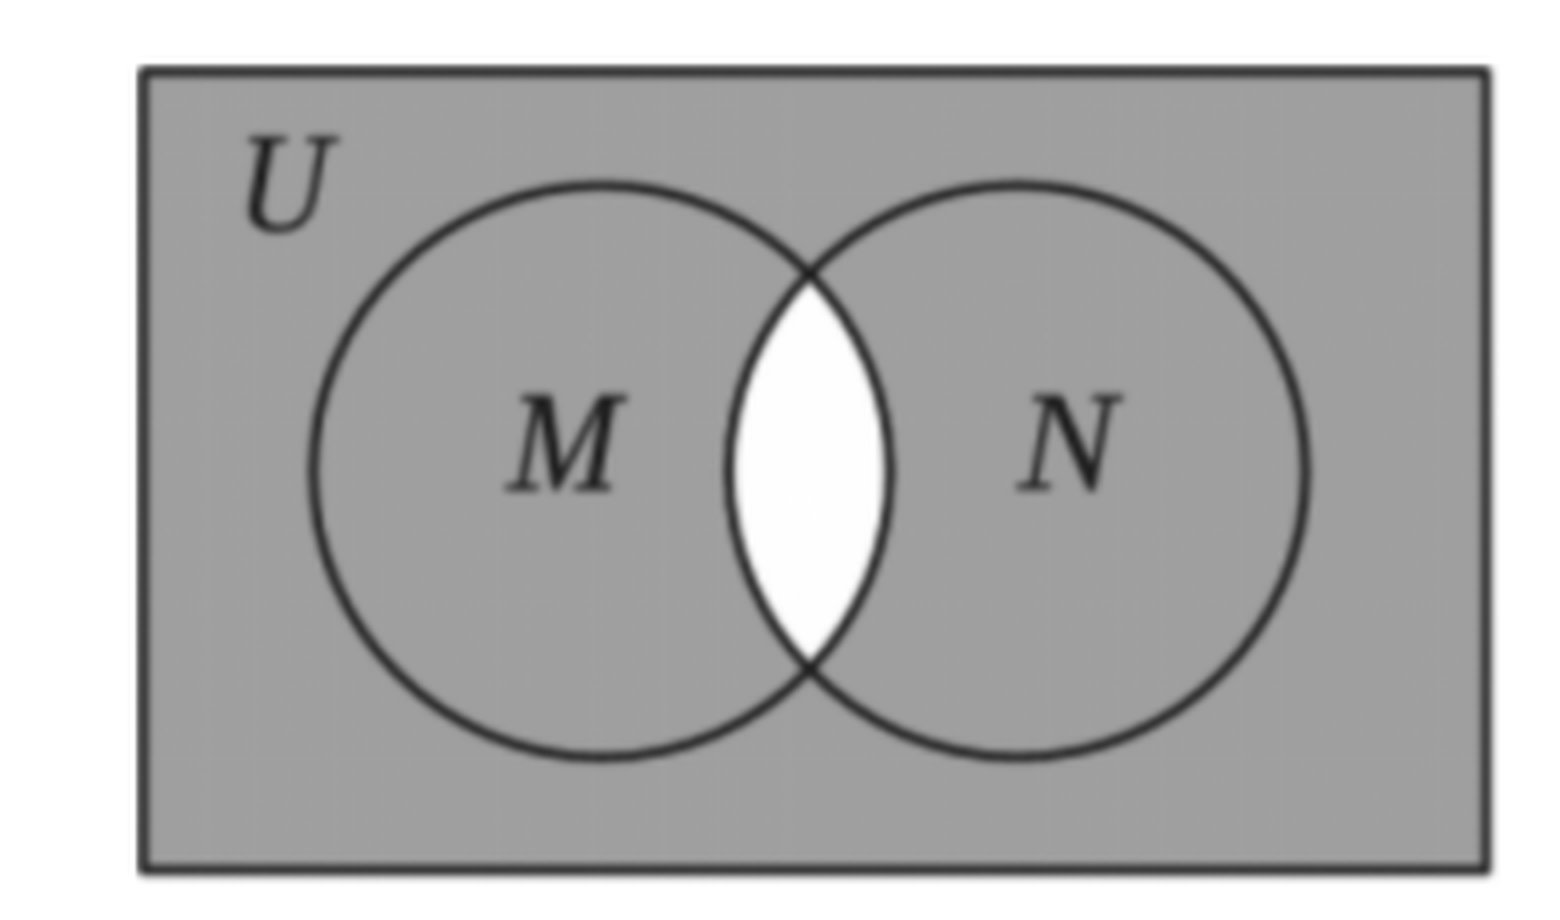
\includegraphics[width=0.40\textwidth]{figures/gao145_q14.png}
\end{center}

\ifanswer
\solbegin
\step{由韦恩图得图中白色区域为集合 $M\cap N$，所以阴影部分表示的集合为 $\overline{M\cap N}$.}
\step{故选 $D$.}
\solend
\fi

% === Q15 ===
\item 已知 $x>-2$，则 $x+\dfrac{1}{x+2}$ 的最小值为\mbox{（\quad）}

\keepwithprev
A. 3\qquad B. 2\qquad C. 1\qquad D. 0

\ifanswer
\solbegin
\step{$x>-2$，则 $x+2>0$，}
\step{所以 $x+\dfrac{1}{x+2}=(x+2)+\dfrac{1}{x+2}-2\geqslant2\sqrt{(x+2)\cdot\dfrac{1}{x+2}}-2=0$，}
\step{当且仅当 $x+2=\dfrac{1}{x+2}$，即 $x=-1$ 时取等号，所以 $x+\dfrac{1}{x+2}$ 的最小值为 $0$.}
\step{故选 $D$.}
\solend
\fi

% 第 16 题：题干在 05 页、解析续至 06 页；两幅数轴标根波浪曲线是【解析】内配图，
% 仅答案版出，放在答案版条件块内 \solbegin 的 \step 之间（照 高一73 第 16 题成例）
\item 关于 $x$ 的不等式 $\dfrac{(x-a)(x-2)^2}{(x-1)(x-5)}\leqslant0$ 的解集中恰有 3 个正整数，则实数 $a$ 的取值范围是\mbox{（\quad）}

\keepwithprev
A. $(-\infty,3]\cup[7,8)$\qquad B. $(-\infty,3)\cup[7,8)$\qquad C. $(-\infty,3]\cup(7,8]$\qquad D. $(-\infty,3)\cup(7,8]$

\ifanswer
\solbegin
\step{由题意，不等式 $\dfrac{(x-a)(x-2)^2}{(x-1)(x-5)}\leqslant0$，}
\step{可化为 $\begin{cases}(x-1)(x-2)^2(x-5)(x-a)\leqslant0\\x\ne1\text{且}x\ne5\end{cases}$，由数轴标根法，}
\step{当 $a=3$ 时，}
\begin{center}
% a=3 数轴标根图取 06 页，去粉色水印、去色、4× LANCZOS 放大；仅答案版出
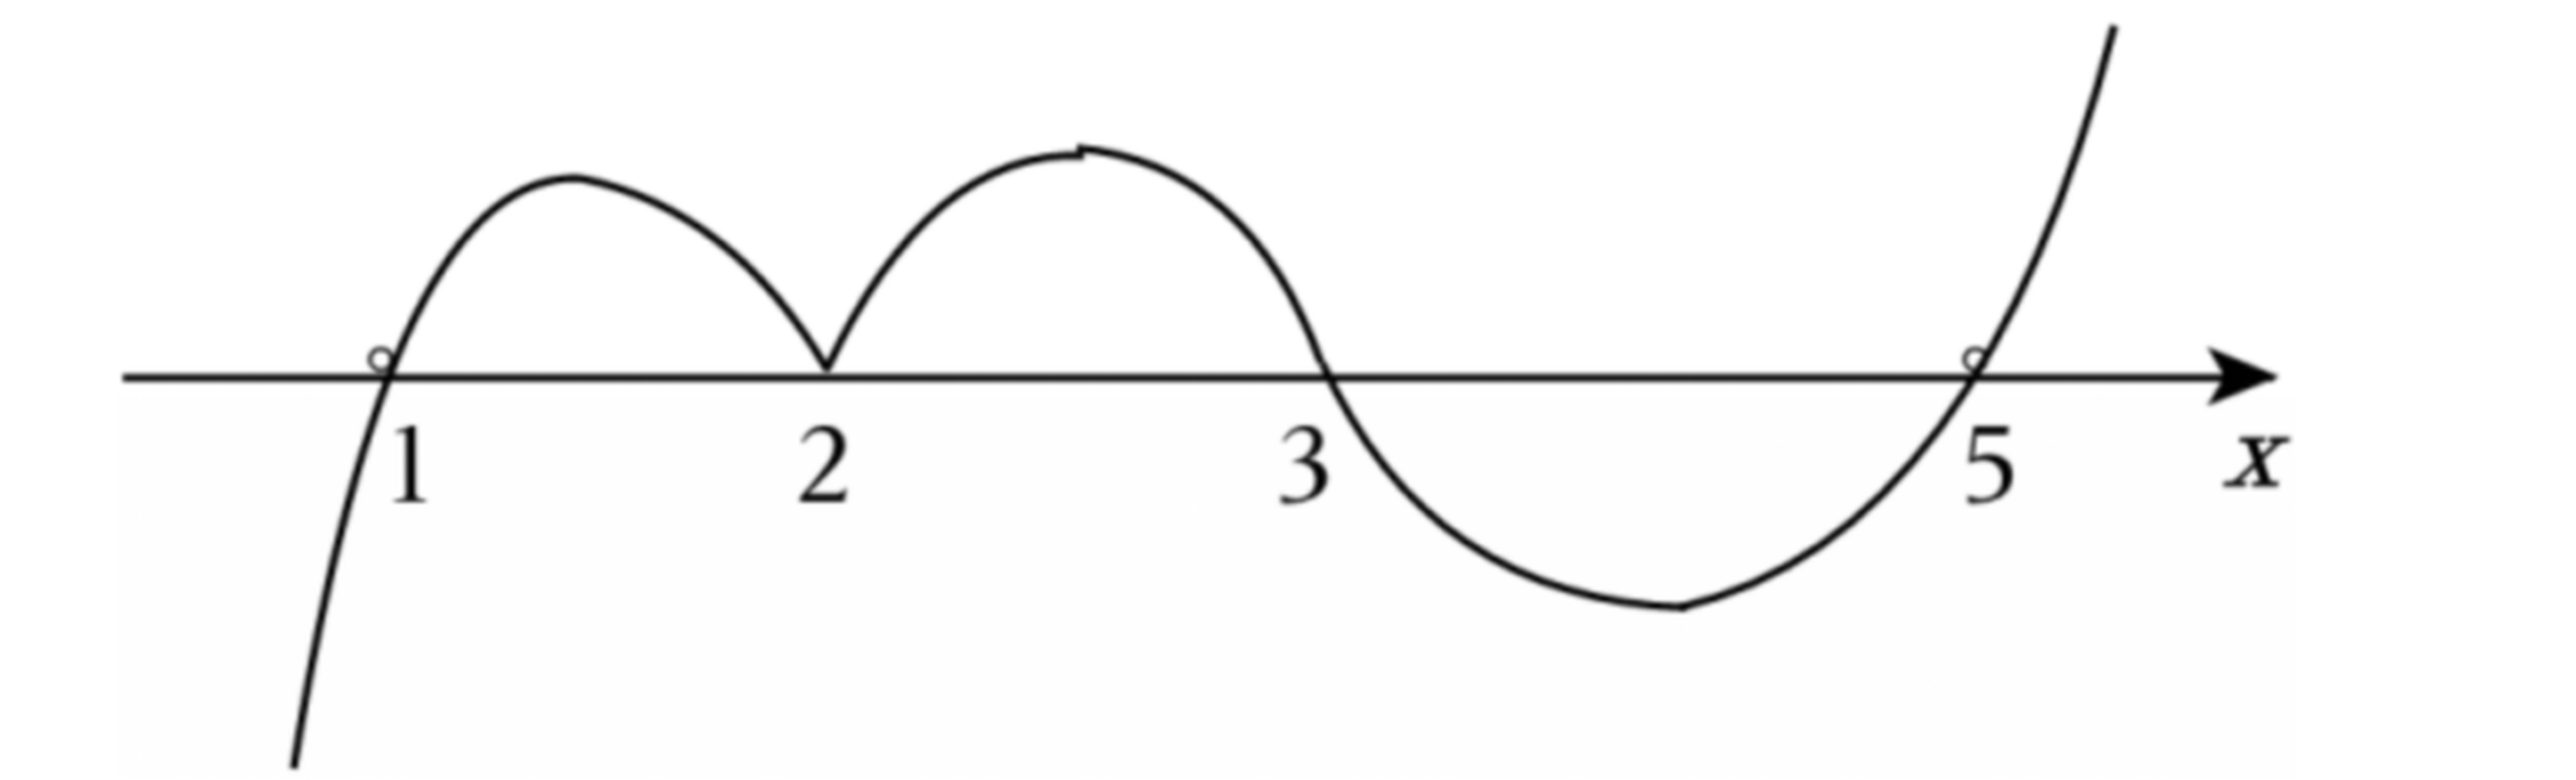
\includegraphics[width=0.62\textwidth]{figures/gao145_q16_a3.png}
\end{center}
\step{得不等式的解集为 $\{x\mid x<1\text{ 或 }x=2\text{ 或 }3\leqslant x<5\}$，}
\step{对应的正整数解为 $2$，$3$，$4$，满足题意，故排除 $B$、$D$；}
\step{当 $a=7$ 时，}
\begin{center}
% a=7 数轴标根图取 06 页，去粉色水印、去色、4× LANCZOS 放大；仅答案版出
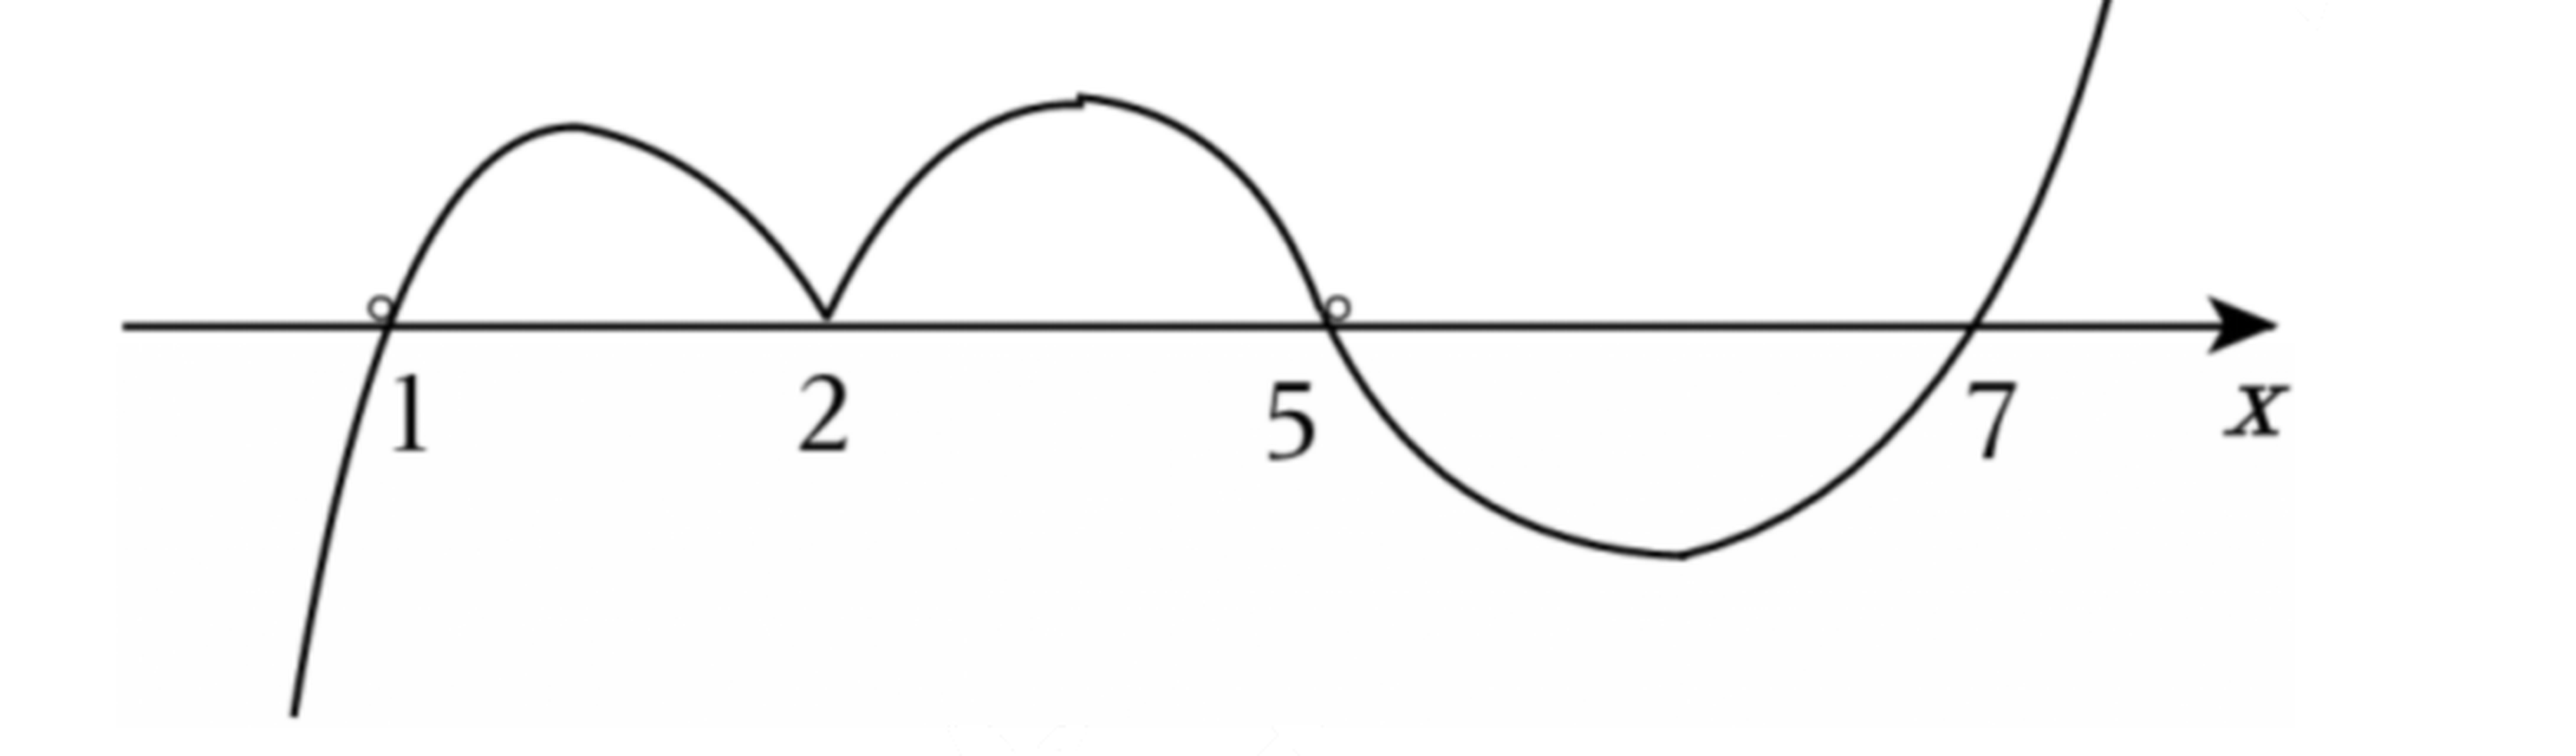
\includegraphics[width=0.62\textwidth]{figures/gao145_q16_a7.png}
\end{center}
\step{得不等式的解集为 $\{x\mid x<1\text{ 或 }x=2\text{ 或 }5<x\leqslant7\}$，}
\step{对应的正整数解为 $2$，$6$，$7$，满足题意，故 $A$ 正确，$C$ 错误.}
\step{故选 $A$.}
\solend
\fi

\end{enumerate}

\bigsec{三、解答题}

\begin{enumerate}
\setcounter{enumi}{16}

% 第 17 题：题干在 06 页、解析续至 07 页，按印刷行断，共 7 行；
% "lg(10÷5)" 的除号照录 \div
\item (1) 已知 $a+a^{-1}=6$，求 $a^2+a^{-2}$ 及 $a^{\frac12}-a^{-\frac12}$ 的值；

(2) 已知 $\lg5=a$，$\lg6=b$，用 $a$、$b$ 分别表示 $\lg2$、$\lg3$、$\lg300$ 和 $\log_{12}15$.

\ifanswer
\solbegin
\step{(1) 因为 $a+a^{-1}=6$，}
\step{所以 $a^2+a^{-2}=(a+a^{-1})^2-2\cdot a\cdot a^{-1}=6^2-2=34$，}
\step{因为 $\left(a^{\frac12}-a^{-\frac12}\right)^2=a-2+a^{-1}=6-2=4$，所以 $a^{\frac12}-a^{-\frac12}=\pm2$；}
\step{(2) $\lg2=\lg(10\div5)=\lg10-\lg5=1-a$，}
\step{$\lg3=\lg(6\div2)=\lg6-\lg2=b-(1-a)=a+b-1$，}
\step{$\lg300=\lg(3\times10^2)=\lg3+\lg10^2=a+b-1+2=a+b+1$，}
\step{所以 $\log_{12}15=\dfrac{\lg15}{\lg12}=\dfrac{\lg3+\lg5}{\lg3+\lg2^2}=\dfrac{a+b-1+a}{a+b-1+2(1-a)}=\dfrac{2a+b-1}{b-a+1}$.}
\solend
\fi

% 第 18 题：题干在 07 页、解析续至 08 页（2 问、分类讨论很长），按印刷行断共 25 行；
% 本卷 Q18 用"图像"（Q13/Q14 用"图象"），逐处照录不统一
\item 已知 $f(x)=(m^2-3m+1)x^{m^2-4m-1}$，$y=f(x)$ 为幂函数且在 $(0,+\infty)$ 上是严格减函数.

(1) 求实数 $m$ 的值以及相应的函数表达式；

(2) 若 $y=f(x)$ 的图像关于 $y$ 轴对称，解关于 $x$ 的不等式 $(x+2)^{1-m}<(3x-1)^{1-m}$.

\ifanswer
\solbegin
\step{(1) 由幂函数的定义得 $m^2-3m+1=1$，}
\step{整理得 $m^2-3m=0$，解得 $m=0$ 或 $m=3$，}
\step{由于 $y=f(x)$ 在 $(0,+\infty)$ 上为严格减函数，}
\step{因此幂函数的指数需满足 $m^2-4m-1<0$，}
\step{当 $m=3$ 时，指数为 $3^2-4\times3-1=-4<0$，满足严格递减条件，}
\step{此时函数表达式为 $f(x)=x^{-4}$，}
\step{当 $m=0$ 时，指数为 $0^2-4\times0-1=-1<0$，满足严格递减条件，}
\step{此时函数表达式为 $f(x)=x^{-1}$，}
\step{所以满足条件的实数 $m$ 为 $0$ 或 $3$，}
\step{对应的函数表达式分别为 $f(x)=x^{-1}$、$f(x)=x^{-4}$；}
\step{(2) 函数图像关于 $y$ 轴对称即函数为偶函数，}
\step{对于 $f(x)=x^{-1}=\dfrac1x$，定义域为 $(-\infty,0)\cup(0,+\infty)$，}
\step{满足 $f(-x)=-f(x)$，为奇函数，图像关于原点对称，}
\step{不满足关于 $y$ 轴对称的条件；}
\step{对于 $f(x)=x^{-4}=\dfrac{1}{x^4}$，定义域为 $(-\infty,0)\cup(0,+\infty)$，}
\step{满足 $f(-x)=f(x)$，为偶函数，图像关于 $y$ 轴对称，}
\step{因此符合条件的 $m$ 值为 $3$，}
\step{将 $m=3$ 代入关于 $x$ 的不等式 $(x+2)^{1-m}<(3x-1)^{1-m}$，}
\step{得 $(x+2)^{1-3}<(3x-1)^{1-3}$，即 $(x+2)^{-2}<(3x-1)^{-2}$，}
\step{因为负指数幂的底数不能为 $0$，所以 $x+2\ne0$ 且 $3x-1\ne0$，}
\step{即 $x\ne-2$ 且 $x\ne\dfrac13$，}
\step{不等式可变形为 $\dfrac{1}{(x+2)^2}<\dfrac{1}{(3x-1)^2}$，}
\step{整理得 $(3x-1)^2<(x+2)^2$，即 $8x^2-10x-3<0$，}
\step{解得 $-\dfrac14<x<\dfrac32$，又 $x\ne-2$ 且 $x\ne\dfrac13$，}
\step{所以不等式的解集为 $\left(-\dfrac14,\dfrac13\right)\cup\left(\dfrac13,\dfrac32\right)$.}
\solend
\fi

% 第 19 题：题干在 08 页、解析续至 09 页，按印刷行断，共 14 行；
% 判别式 cases 块内"△=4a²−16a<0"原卷印扁等边三角 \triangle
%（放大 09 页 zz09_delta.png 与 Q12 高 \Delta 并排确认），逐处照录不统一
\item 已知 $f(x)=ax^2+2ax+4$，$a\in\R$.

(1) 若关于 $x$ 的不等式 $f(x)>0$ 在实数集 $\R$ 上恒成立，求实数 $a$ 的取值范围；

(2) 当 $a<0$ 时，解关于 $x$ 的不等式 $f(x)>(a+1)x+5$.

\ifanswer
\solbegin
\step{(1) 由题意得，关于 $x$ 的不等式 $f(x)>0$ 在实数集 $\R$ 上恒成立，}
\step{即 $ax^2+2ax+4>0$ 在实数集 $\R$ 上恒成立，}
\step{当 $a=0$ 时，不等式为 $4>0$ 恒成立，符合题意；}
\step{当 $a\ne0$ 时，则 $\begin{cases}a>0\\\triangle=4a^2-16a<0\end{cases}$，解得 $0<a<4$.}% 判别式原卷印扁等边三角 $\triangle$，照录
\step{综上所述，实数 $a$ 的取值范围为 $[0,4)$.}
\step{(2) $f(x)=ax^2+2ax+4$，}
\step{当 $a<0$ 时，不等式 $f(x)>(a+1)x+5$ 即为 $ax^2+(a-1)x-1>0$，}
\step{即 $(ax-1)(x+1)>0$，即 $\left(x-\dfrac1a\right)(x+1)<0$，}
\step{当 $a<-1$，即 $\dfrac1a>-1$ 时，解得 $-1<x<\dfrac1a$；}
\step{当 $a=-1$，即 $\dfrac1a=-1$ 时，解得 $x\in\varnothing$；}
\step{当 $-1<a<0$，即 $\dfrac1a<-1$ 时，解得 $\dfrac1a<x<-1$.}
\step{综上所述，当 $a<-1$ 时，不等式的解集为 $\left\{x\mid -1<x<\dfrac1a\right\}$；}
\step{当 $a=-1$ 时，不等式的解集为 $\varnothing$；}
\step{当 $-1<a<0$ 时，不等式的解集为 $\left\{x\mid \dfrac1a<x<-1\right\}$.}
\solend
\fi

% 第 20 题：菜园靠墙图为题目配图（三版都出），题干写"如图"；
% 题干在 09 页（含图）、解析续至 10 页，按印刷行断，共 13 行
\needvspace{8cm}
\item 如图，某人计划用篱笆围成一个一边靠墙（墙足够长）的矩形菜园. 设菜园的长为 $x$ 米，宽为 $y$ 米.

\begin{center}
% 矩形菜园靠墙图取 09 页右下，去粉色水印、去色、4× LANCZOS 放大
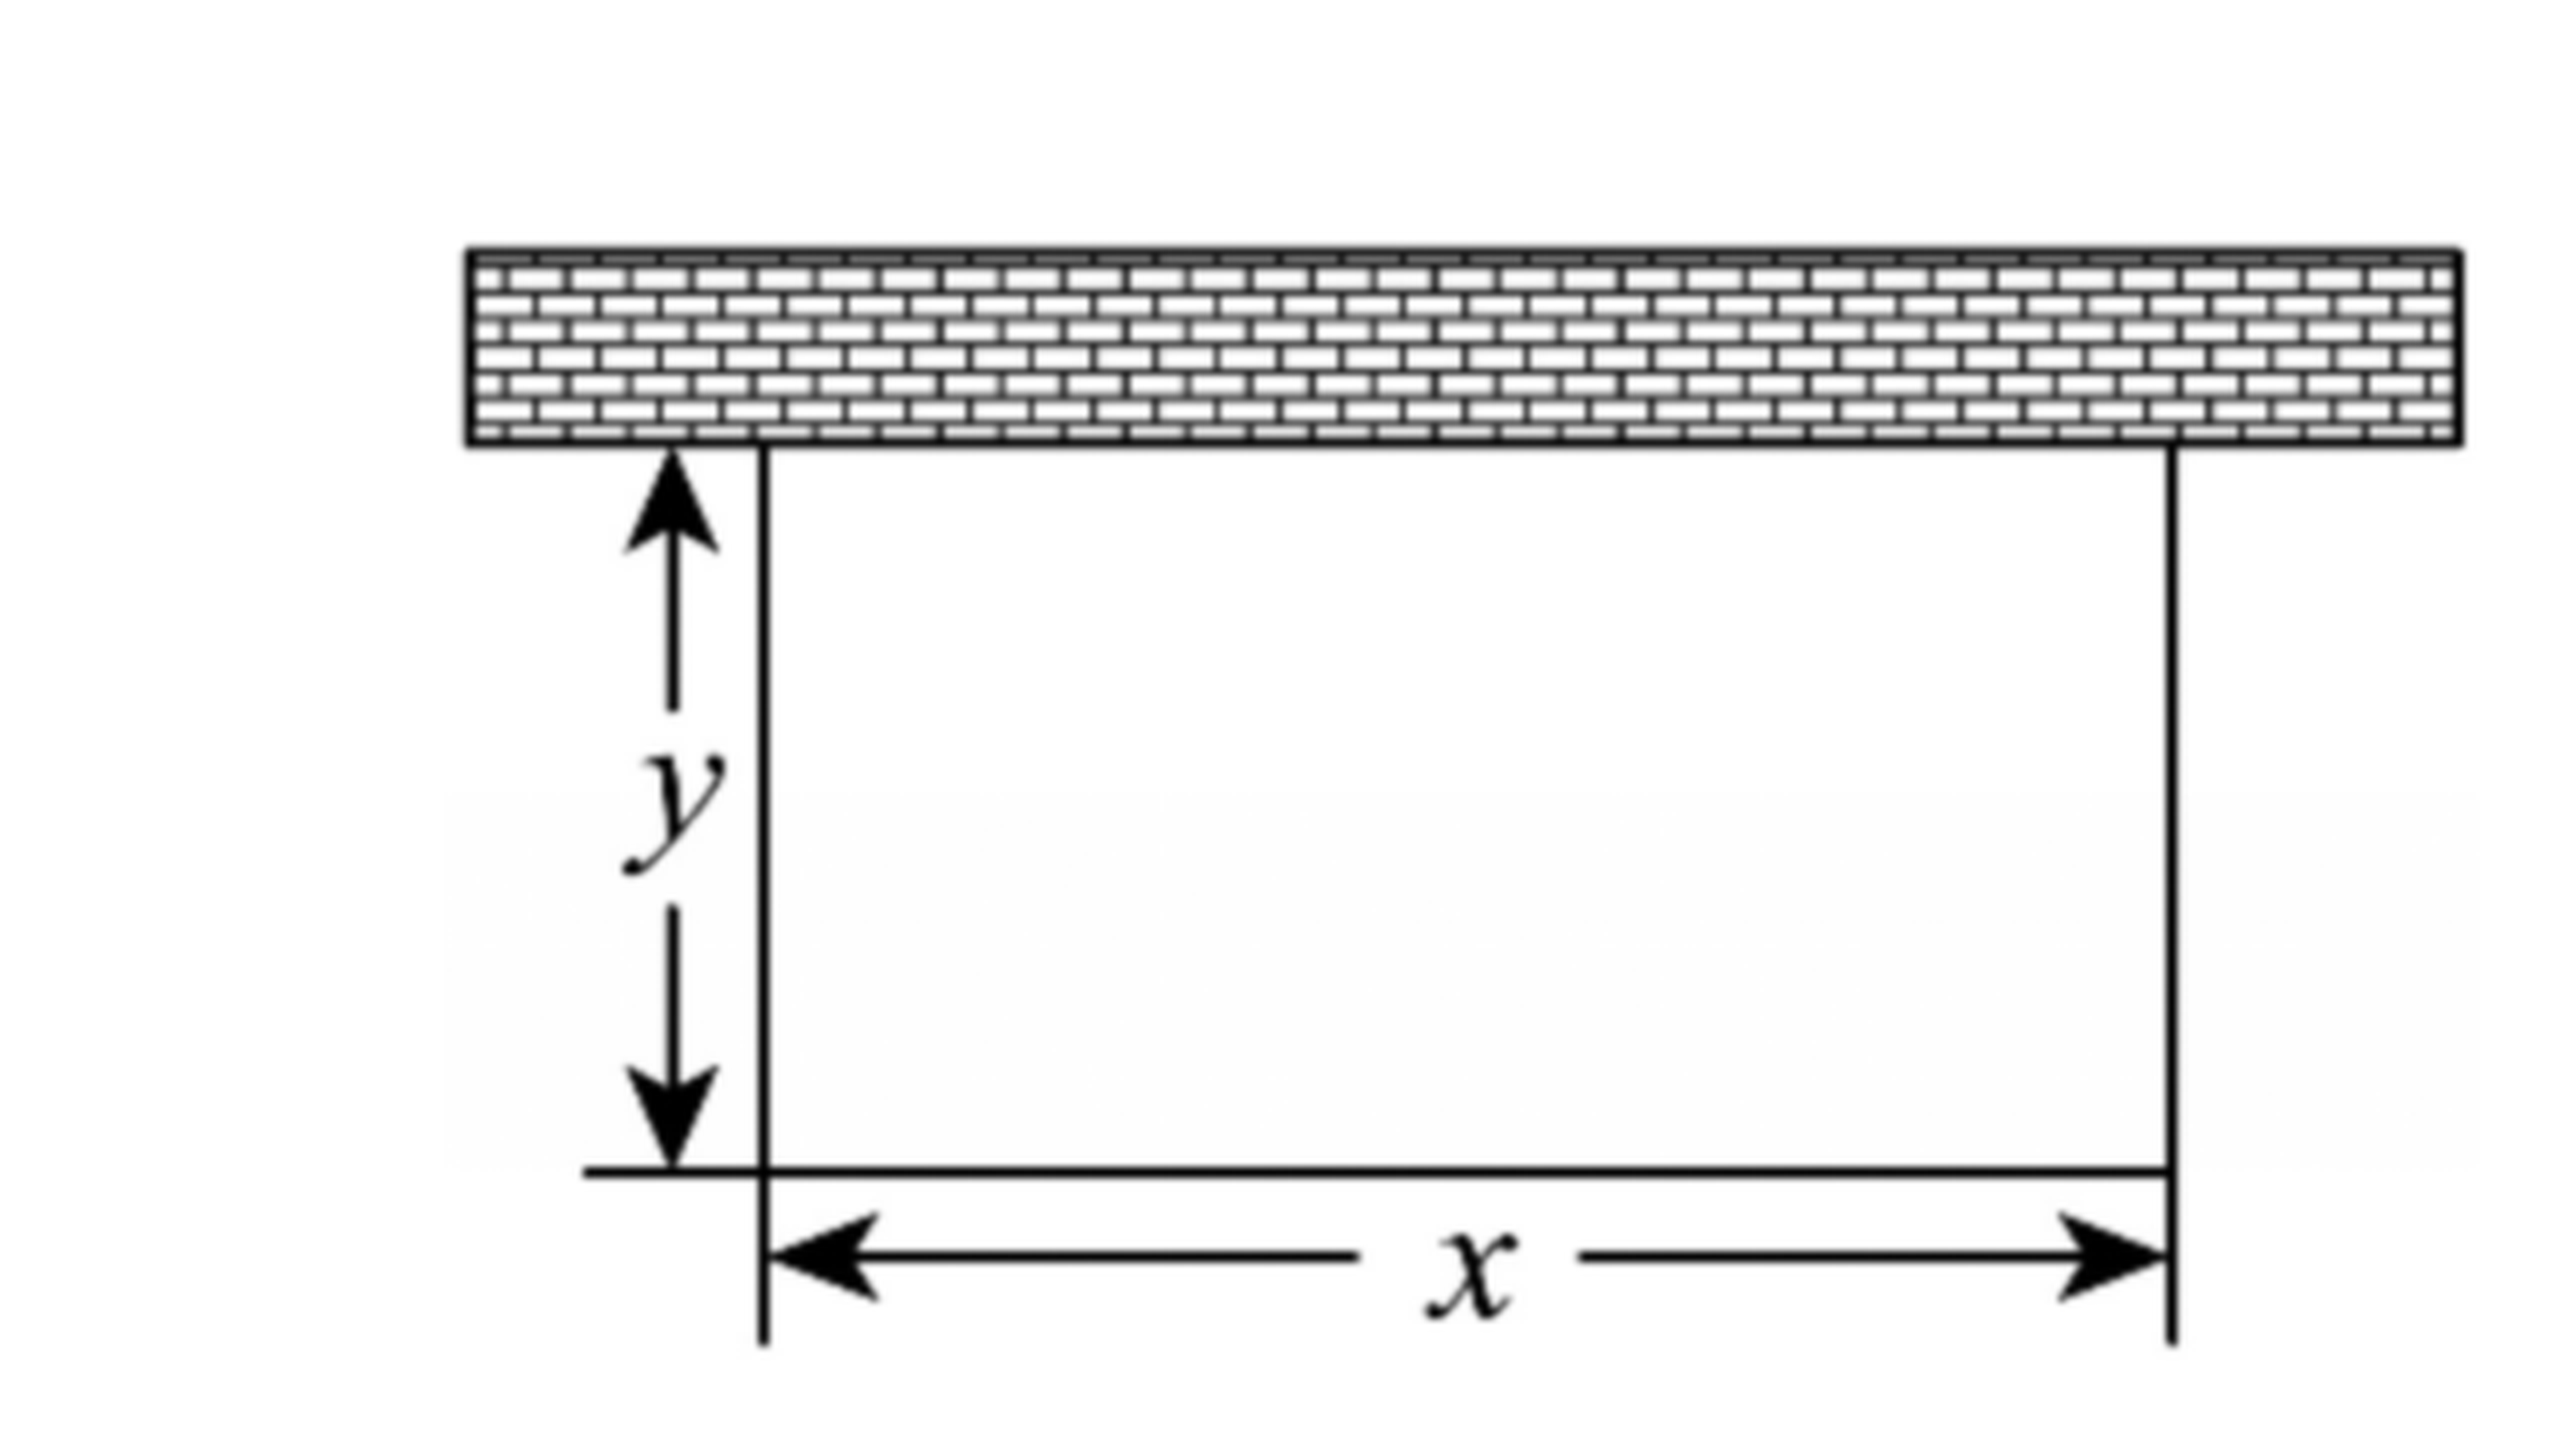
\includegraphics[width=0.55\textwidth]{figures/gao145_q20.png}
\end{center}

(1) 若菜园面积为 72 平方米，则 $x$、$y$ 为何值时，所用篱笆总长最小？

(2) 若 $x$、$y$ 满足 $x+y-xy+63=0$，则菜园面积最小为多少平方米？

\ifanswer
\solbegin
\step{(1) 由题意得，菜园的面积 $S=xy=72$，且 $x>0$，$y>0$，}
\step{所用篱笆总长 $L=x+2y$，}
\step{由基本不等式得 $x+2y\geqslant2\sqrt{x\cdot2y}=2\sqrt{2xy}=2\sqrt{2\times72}=24$，}
\step{当且仅当 $x=2y$ 时取等号，}
\step{联立 $\begin{cases}xy=72\\x=2y\end{cases}$，解得 $\begin{cases}x=12\\y=6\end{cases}$，}
\step{所以当 $x=12$，$y=6$ 时，所用篱笆总长最小；}
\step{(2) 由题意得 $x>0$，$y>0$，且满足 $x+y-xy+63=0$，即 $x+y=xy-63$，}
\step{由基本不等式得 $x+y\geqslant2\sqrt{xy}$，当且仅当 $x=y$ 时取等号，}
\step{所以 $xy-63\geqslant2\sqrt{xy}$. 令 $t=\sqrt{xy}(t>0)$，则 $xy=t^2$，}
\step{上述不等式可化为 $t^2-2t-63\geqslant0$，即 $(t-9)(t+7)\geqslant0$，}
\step{因为 $t>0$，所以 $t+7>0$，故 $t-9\geqslant0$，解得 $t\geqslant9$，所以 $\sqrt{xy}\geqslant9$，}
\step{即 $xy\geqslant81$，当且仅当 $x=y=9$ 时取等号，此时满足 $9+9-81+63=0$，}
\step{所以菜园面积最小为 81 平方米.}
\solend
\fi

% 第 21 题：题干在 10 页、解析续至 11 页（3 问、分类讨论很长），按印刷行断共 22 行；
% 末行"故第 2026 个元素是 2700 之后第一个属于 A 的数，即 2701." 为全卷收尾，
% 无 Q22/Q23、无附加题节；数集 Z/N* 按全稿惯例改 \Z/\N^*
\item 已知集合 $A=\{x\mid x=m^2-n^2$，$m$、$n\in\Z\}$.

(1) 求证：任何奇数 $2k+1(k\in\Z)$ 都是集合 $A$ 中的元素；

(2) 判断偶数 $4k-2(k\in\Z)$ 是否为集合 $A$ 的元素？请说明理由；

(3) 若将集合 $A$ 中的正整数由小到大排列，求出集合 $A$ 中第 2026 个正整数.

\ifanswer
\solbegin
\step{(1) 因为 $x=(k+1)^2-k^2=2k+1(k\in\Z)$，}
\step{所以任何奇数 $2k+1(k\in\Z)$ 都属于集合 $A$；}
\step{(2) 偶数 $4k-2(k\in\Z)$ 不是集合 $A$ 的元素，理由如下：}
\step{由题意得 $x=m^2-n^2=(m-n)(m+n)$，}
\step{当 $m$、$n$ 均为奇数时，设 $m=2k_1+1$，$n=2k_2+1(k_1$、$k_2\in\Z)$，}
\step{则 $m^2-n^2=(2k_1+1)^2-(2k_2+1)^2=(2k_1-2k_2)(2k_1+2k_2+2)$}
\step{$=4(k_1-k_2)(k_1+k_2+1)$，}
\step{因为 $k_1$、$k_2\in\Z$，所以 $k_1-k_2\in\Z$，$k_1+k_2+1\in\Z$，}
\step{从而 $m^2-n^2$ 为 $4$ 的倍数；}
\step{当 $m$、$n$ 均为偶数时，设 $m=2k_1$，$n=2k_2(k_1$、$k_2\in\Z)$，}
\step{$m^2-n^2=4k_1^2-4k_2^2=4(k_1^2-k_2^2)$ 为 $4$ 的倍数；}
\step{当 $m$、$n$ 为一个偶数一个奇数时，不妨设 $m$ 为偶数，$n$ 为奇数，}
\step{设 $m=2k_1$，$n=2k_2+1(k_1$、$k_2\in\Z)$，}
\step{则 $m^2-n^2=4k_1^2-(2k_2+1)^2=4(k_1^2-k_2^2-k_2)-1$ 为奇数.}
\step{无论哪种情况均不满足 $4k-2(k\in\Z)$，}
\step{故偶数 $4k-2(k\in\Z)$ 不是集合 $A$ 的元素；}
\step{(3) 由前两问得，$4$ 的倍数和奇数属于集合 $A$ 中的元素，}
\step{令集合 $A$ 中的正整数元素为 $4k-3$、$4k-1$、$4k(k\in\N^*)$，}
\step{对任意的 $k\in\N^*$，连续的 $4$ 个整数 $4k-3$、$4k-2$、$4k-1$、$4k$ 中}
\step{有三个数 $4k-3$、$4k-1$、$4k$ 都在集合 $A$ 中，}
\step{因为 $2026=3\times675+1$，所以集合 $A$ 中第 $2025$ 个元素为 $4\times675=2700$，}
\step{故第 2026 个元素是 2700 之后第一个属于 $A$ 的数，即 2701.}
\solend
\fi

\end{enumerate}

\end{document}
"
%
% ① 原始材料：微信公众号"魔都数学加油站"文章，连载"27学年高一145"，原文标题
% "27学年高一145——2026-2027年上海市市二中学高一上期中"；
% 原文链接：https://mp.weixin.qq.com/s/6V-i9KE0GWodC-wmd5z8nQ 。
% 正文为 11 张 PNG 页（01/02/03/08/10/11 为 4762×6735，04/05/06/07/09 为 2560×3620，
% 同一篇各页分辨率不同，逐页按各自分辨率裁图核对，别按预览比例换算裁框）。
% 题目下印【答案】或【解析】，为混合体例讲评版：Q3 只印【答案】、无【解析】，其余
% 18 题印【解析】。题目、解析均据原图转录；卷面粉红色水印"魔都数学加油站"及
% 公众号页脚未录入。
% 全卷插图情况（逐页通读 11 页确认，题干写"如图"处均配有图）：
%   · Q14 韦恩图（05 页右侧，全集 U 矩形＋两圆 M/N＋白色交集、灰色阴影＋U/M/N 标注）：
%     题目配图（选择题选项旁），三版都出，裁自 05 页去水印去色 4× 放大存
%     figures/gao145_q14.png；
%   · Q16 两幅数轴标根波浪曲线（06 页，a=3 与 a=7 各一幅，标根法画
%     (x-1)(x-2)^2(x-5)(x-a)≤0 的符号曲线）：【解析】内的配图，仅答案版出，
%     裁 figures/gao145_q16_a3.png / figures/gao145_q16_a7.png（或合并一张），
%     放在答案版条件块内 \solbegin 的 \step 之间（照 高一73 第 16 题成例）；
%   · Q20 矩形菜园靠墙图（09 页右下，灰色砖墙＋矩形菜园＋x/y 标注＋箭头）：
%     题目配图，三版都出，裁自 09 页去水印去色 4× 放大存 figures/gao145_q20.png；
%   其余各页逐页确认无其它题目配图、无表格、亦无"题干写如图而源码漏图"一处。
%
% 卷首标题：原卷印作"2026-2027 年市二中学高一上期中"，年份区间按全稿惯例排 en dash；
% 原卷卷面未印副标题，本稿按同期中卷（高一140／141／143／144）知识模块口径补出
% "集合与常用逻辑用语、不等式、函数"。
%
% 题号体例：本卷共 19 题——一、填空题 3—12（10 题）、二、选择题 13—16（4 题）、
% 三、解答题 17—21（5 题）。三节分别 \setcounter{enumi}{2}／{12}／{16}。
% 原卷从第 3 题起、无第 1、2 题，本稿保留原题号；全卷无附加题节。
%
% ② 与原卷的排版差异：
%   ① 原文从第 3 题起，本稿保留原题号；共 19 题三节；
%   ② 混合体例：原卷 Q3 只印【答案】、无【解析】（"第一步应假设___。
%      【答案】x≤2 或 y≤2"），按 高一140 第 5 题成例提 \ans{}、不补造解析；
%      其余 18 题印【解析】，用 \solbegin…\solend，选择题答案在解析末句"故选 X"
%      （Q13 选 B、Q14 选 D、Q15 选 D、Q16 选 A，逐个放大原图核实）、
%      题干括号 \mbox{（\quad）} 留空、不另提 \ans{}；填空／解答答案落在解析里；
%      答案版【答案】/【解析】标记数 = 19（1 个 \ans ＋ 18 个 \solbegin）= 全卷题数；
%   ③ 原卷卷面未印副标题，本稿按知识模块口径补出；
%   ④ 原卷填空横线按全稿惯例排 \blankline[4.4em]；选择题括号排 \mbox{（\quad）}、
%      选项段前按惯例加 \keepwithprev；解答题不留作答区、不加 \anspace
%      （原卷为讲评版，与 129／131／132／133／136／140／141／143／144 同）；
%   ⑤ 数集：Q9"a、b∈R"、Q12"a∈R"、Q21"m、n∈Z""k∈Z""k∈N*"等原卷印
%      斜体或黑板粗体 R/Z/N，按全稿惯例统一改 \R／\Z／\N^*；绝对值排 \lvert…\rvert，
%      集合描述竖线排 \mid；不等号按全稿惯例排 \leqslant／\geqslant；
%      补集照原卷上划线排 \overline{M}／\overline{N}（Q14 选项 B/C/D 逐处核）；
%      空集记号 \varnothing；\subset（单线⊂）与 \subseteq（带下划线⊆）逐处照录不统一；
%   ⑥ 子题标号 (1)(2)(3) 原卷印半角括号照录；圈数字进数学式用 \text{①}（否则 FONTCHK 挂）；
%      \left…\right 不得拆到不同 $…$ 组；cases 块整体算一个印刷行；
%   ⑦ 题干／解析中的中文弯引号按原卷照录（Q3"若 x+y>4，则 x>2 且 y>2"、
%      Q11"a₁/a₂=b₁/b₂""M=N"、选填"充分非必要""必要非充分""充要""既非充分也非必要"
%      等，含引号内空格），注释内一律 ASCII 引号；数学式内 CJK 用 \text{}；
%   ⑧ 半角逗号在数学组之间是全稿惯例、非笔误（如 Q5"x₁+x₂=6，x₁x₂=√3"、
%      Q7"a>1，b>1"、指数／对数式内逗号），逐处照录别改全角；行末西文句点照录为
%      ASCII `.`；行中全角逗号／顿号照录；
%   ⑨ "图像／图象"逐处照录不统一（Q18"图像关于 y 轴对称"等，核全卷）；
%   ⑩ 判别式 Δ/△ 混用是照录项：Q12 解析"Δ=a²−4a²(2a−3)>0"、
%      Q19 解析"Δ=4a²−16a<0"等，放大原图判断是高 \Delta（等腰偏高、高>宽）
%      还是扁 \triangle，逐处照录不得统一（参照 高一142／144 头注④口径）；
%   ⑪ 一条 \step = 原卷解析的一个印刷行，cases 块整体算一个印刷行；别把原卷折行
%      并起来、别把一行拆多条。Q6 分段讨论、Q12 三个 cases 条件组、Q16 数轴标根、
%      Q18／Q19 分类讨论、Q21 三问均按印刷行逐条断，不丢行；
%   ⑫ Q14 韦恩图为"题干＋选项＋图"整块，加 \needvspace 守卫推走（守卫放 \item 之前，
%      见 高一140 Q14、高一144 Q17 成例与切页审计 B 类坑）；Q20 菜园图同理；
%      三版切页审计均"合计异常：无"；
%   ⑬ 跨页续印按题合并：Q3/4/5/6 在 01 页（Q6 解析续 02 页顶）；Q7/8/9/10 在 02 页
%      （Q10 解析续 03 页）；Q11/12 在 03 页（Q12 解析续 04 页，很长）；
%      Q13 在 04 页末、解析在 05 页顶；Q14/15/16 在 05 页（Q16 解析续 06 页含两幅数轴图）；
%      Q17 在 06 页、解析续 07 页；Q18 在 07 页、解析续 08 页；Q19 在 08 页、解析续 09 页；
%      Q20 在 09 页（含菜园图）、解析续 10 页；Q21 在 10 页、解析续 11 页
%      （末页收尾"故第 2026 个元素是 2700 之后第一个属于 A 的数，即 2701."、
%      无 Q22/Q23、无附加题节）。本稿按题连排，不丢行、不并折行；
%   ⑭ 原卷解析内若有红色"法一／法二"之类小标题，按全稿惯例排 \stepm{标签}{…}
%      （黑体着色、不引入红色、不改 common.sty），头注注明；水印"魔都数学加油站"
%      红色不录入。
%
% ③ 行数复核：一条 \step／\stepm = 原卷解析的一个印刷行，cases 块作一个印刷行计。
%   逐题数（主会话逐页核对定稿）：Q3：0（只印【答案】、提 \ans{}，不计入 \step 账）；
%   Q4：3；Q5：2；Q6：10；Q7：3；Q8：3；Q9：2；Q10：7；Q11：4；Q12：12；
%   Q13：2；Q14：2；Q15：4；Q16：9；Q17：7；Q18：25；Q19：14；Q20：13；Q21：22。
%   合计 144 条 \step（本卷无 \stepm：解析内无红色"法一／法二"类小标题），
%   与原卷逐题印刷行相等。全卷 18 题设 \solbegin…\solend ＋ Q3 一处 \ans{}，
%   答案版【答案】/【解析】标记数 = 19 = 全卷题数。
%
% ④ 判别式／子集符号结论（逐处放大原图照录、不得统一，主会话像素级复核）：
%   判别式全卷 2 处、两形混用逐处照录不统一（参照 高一142／144 头注④口径）：
%     · Q12 解析 cases 块"Δ=a²−4a²(2a−3)>0" 原卷印等腰偏高粗三角（高>宽），
%       照录 \Delta（放大 04 页 /tmp/gao145s2/main_q12_delta.png 确认）；
%     · Q19 解析 cases 块"△=4a²−16a<0" 原卷印扁等边空心三角（宽≈高、细线），
%       照录 \triangle（放大 09 页 /tmp/gao145s2/main_q19_delta.png 确认）。
%   子集／补集：Q14 选项 A `M\cup N`、B `M\cap\overline{N}`（上划线只在 N 上）、
%   C `\overline{M\cup N}`（罩整个 M∪N）、D `\overline{M\cap N}`（罩整个 M∩N，
%   非 \overline{M}\cap N；放大 05 页 /tmp/gao145s2/main_q14_opts.png 确认），
%   阴影为灰色区域＝全集减白色交集，答案 D，照录 \overline{M\cap N}；
%   全集卷无 \subset／\subseteq 混用（本卷集合题用 \cup／\cap／\overline{}）；
%   空集 \varnothing（Q19 解析 x∈\varnothing）；数集 \R／\Z／\N^* 归一见 ② ⑤。
%
% ⑤ 存疑照录（放大原图确认，照录未改、正文对应处另有 % 注）：
%   1. Q3 题干"若 x+y>4，则 x>2 且 y>2" 后"时"前留一空格、弯引号内空格照录；
%      该卷混合体例（Q3 只印【答案】、提 \ans{}）见 ② ②。
%   2. Q4／Q5 解析中的"1，3，5 和 6"、"x₁+x₂=6,x₁x₂=√3" 等半角／全角逗号
%      逐处照原卷（放大 01 页确认），数学式内半角逗号为全稿惯例、非笔误。
%   3. Q14 选项 D 上划线罩住整个 M∩N（而非仅罩 M），照录 \overline{M\cap N}。
%   4. Q12 判别式高 \Delta 与 Q19 判别式扁 \triangle 两形混用，逐处照录不统一（见 ④）。
%   全卷除此 4 类外未发现其它笔误／自相矛盾处。
%
% ⑥ 跨页续印按题合并说明：见 ② ⑬。
%
\documentclass[a4paper,11pt]{article}
\usepackage{common}

\begin{document}

\examtitlest[3]{2026--2027 年市二中学高一上期中}{集合与常用逻辑用语、不等式、函数}

\bigsec{一、填空题}

\begin{enumerate}
\setcounter{enumi}{2}

% 第 3 题：原卷只印【答案】、无【解析】（放大 01 页确认），按 高一140 第 5 题成例
% 提 \ans{}、不补造解析；题干中文弯引号与"时"前空格照录
\item 用反证法证明命题：“若 $x+y>4$，则 $x>2$ 且 $y>2$” 时，第一步应假设\blankline[4.4em].

\ifanswer
\ans{$x\leqslant2$ 或 $y\leqslant2$}
\fi

% === Q4 ===
\item 设集合 $M$ 满足 $\{1,3,5,6\}\cup M=\{1,2,3,4,5,6\}$，则满足条件的所有 $M$ 的个数为\blankline[4.4em].

\ifanswer
\solbegin
\step{集合 $M$ 满足 $\{1,3,5,6\}\cup M=\{1,2,3,4,5,6\}$，}
\step{则 $M$ 中必含有 $2$ 和 $4$，$1$，$3$，$5$ 和 $6$ 可以选也可不选，}
\step{则满足条件的所有 $M$ 的数目相当于集合 $\{1,3,5,6\}$ 的子集的个数 $2^4=16$.}
\solend
\fi

% === Q5 ===
\item 已知方程 $x^2-6x+\sqrt3=0$ 的两根为 $x_1$ 和 $x_2$，则 $(x_1-x_2)^2=$\blankline[4.4em].

\ifanswer
\solbegin
\step{因为方程 $x^2-6x+\sqrt3=0$ 的两根为 $x_1$ 和 $x_2$，所以 $x_1+x_2=6,x_1x_2=\sqrt3$，}% 数学式内半角逗号为全稿惯例，照录
\step{所以 $(x_1-x_2)^2=(x_1+x_2)^2-4x_1x_2=36-4\sqrt3$.}
\solend
\fi

% 第 6 题：题干在 01 页，解析续至 02 页顶（末 2 行），按印刷行逐条断，共 10 行
\item 不等式 $\lvert x-2026\rvert+\lvert x-2029\rvert>3$ 的解集是\blankline[4.4em].

\ifanswer
\solbegin
\step{当 $x<2026$ 时，$x-2026<0$，$x-2029<0$，}
\step{原不等式可化为 $(2026-x)+(2029-x)>3$，解得 $x<2026$，}
\step{故此时，不等式的解为 $x<2026$；}
\step{当 $2026\leqslant x\leqslant2029$ 时，$x-2026\geqslant0$，$x-2029\leqslant0$，}
\step{原不等式可化为 $(x-2026)+(2029-x)>3$，即 $3>3$，显然不成立，}
\step{故此时，不等式无解；}
\step{当 $x>2029$ 时，$x-2026>0$，$x-2029>0$，}
\step{原不等式可化为 $(x-2026)+(x-2029)>3$，解得 $x>2029$，}
\step{故此时，不等式的解为 $x>2029$.}
\step{综上，原不等式的解集为 $(-\infty,2026)\cup(2029,+\infty)$.}
\solend
\fi

% === Q7 ===
\item 已知 $a>1$，$b>1$，若 $\log_a b+\log_b a=2$，且 $ab=2$，则 $\log_2(a+b)=$\blankline[4.4em].

\ifanswer
\solbegin
\step{由 $\log_a b+\log_b a=2$，$a>1$，$b>1$，得 $\log_a b+\dfrac{1}{\log_a b}=2$，}
\step{即 $(\log_a b)^2-2\log_a b+1=0$，则 $(\log_a b-1)^2=0$，解得 $\log_a b=1$，即 $a=b$，}
\step{又 $ab=2$，所以 $a=b=\sqrt2$，所以 $\log_2(a+b)=\log_2 2\sqrt2=\log_2 2^{\frac32}=\dfrac32$.}
\solend
\fi

% === Q8 ===
\item 已知 $m>0$，$n>0$，且 $m+n=1$，则 $\dfrac1m+\dfrac4n$ 的最小值为\blankline[4.4em].

\ifanswer
\solbegin
\step{由 $m>0$，$n>0$，$m+n=1$，}
\step{则 $\dfrac1m+\dfrac4n=(m+n)\left(\dfrac1m+\dfrac4n\right)=5+\dfrac nm+\dfrac{4m}n\geqslant5+2\sqrt{\dfrac nm\cdot\dfrac{4m}n}=9$，}
\step{当且仅当 $n=2m=\dfrac23$ 时，上式取得等号，故最小值为 $9$.}
\solend
\fi

% === Q9 ===
\item 已知 $a$、$b\in\R$，且 $3a+2b=1$，则 $8^a+4^b$ 最小值为\blankline[4.4em].

\ifanswer
\solbegin
\step{因为 $3a+2b=1$，所以 $8^a+4^b=2^{3a}+2^{2b}\geqslant2\sqrt{2^{3a+2b}}=2\sqrt2$，}
\step{当且仅当 $3a=2b$ 时取等号，故最小值为 $2\sqrt2$.}
\solend
\fi

% 第 10 题：题干在 02 页、解析续至 03 页顶，按印刷行断，共 7 行
\item 已知关于 $x$ 的不等式 $ax^2+bx+c>0$ 的解集为 $\{x\mid 1<x<2\}$，则关于 $x$ 的不等式 $bx^2-ax+c<0$ 的解集为\blankline[4.4em].

\ifanswer
\solbegin
\step{已知关于 $x$ 的不等式 $ax^2+bx+c>0$ 的解集为 $\{x\mid 1<x<2\}$，}
\step{由解集为 $1<x<2$ 且二次函数在两根之间为正，得 $a<0$，两个根为 $1$，$2$，}
\step{所以 $ax^2+bx+c=a(x-1)(x-2)=ax^2-3ax+2a$，}
\step{比较系数得 $b=-3a$，$c=2a$.}
\step{于是 $bx^2-ax+c=-3ax^2-ax+2a=-a(3x-2)(x+1)$，}
\step{$a<0$，故 $bx^2-ax+c<0$ 等价于 $(3x-2)(x+1)<0$，解得 $-1<x<\dfrac23$，}
\step{故 $bx^2-ax+c<0$ 的解集为 $\left\{x\mid -1<x<\dfrac23\right\}$.}
\solend
\fi

% 第 11 题：题干引号内空格照录（放大 03 页确认），四组选填引号亦同；
% 结论"故为必要非充分条件"照录，解析共 4 个印刷行
\item 设 $a_1$、$b_1$、$a_2$、$b_2$ 均为非零实数，不等式 $a_1x+b_1>0$ 和 $a_2x+b_2>0$ 的解集分别为集合 $M$、$N$，那么 “ $\dfrac{a_1}{a_2}=\dfrac{b_1}{b_2}$ ” 是 “ $M=N$ ” 的\blankline[4.4em]条件（选填 “ 充分非必要 ”、“ 必要非充分 ”、“ 充要 ” 和 “ 既非充分也非必要 ”）.

\ifanswer
\solbegin
\step{当 $a_1=b_1=1$，$a_2=b_2=-1$ 时，满足 $\dfrac{a_1}{a_2}=\dfrac{b_1}{b_2}$，}
\step{但是 $M=N$ 不成立，即充分性不成立；}
\step{若 $M=N$ 时，$\dfrac{a_1}{a_2}=\dfrac{b_1}{b_2}$ 一定成立，即必要性成立.}
\step{故为必要非充分条件.}
\solend
\fi

% 第 12 题：题干在 03 页、解析续至 04 页（很长，含 3 个 cases 条件组），
% 按印刷行逐条断共 12 行；cases 块整体算一个印刷行
\item 已知 $f(x)=\dfrac{ax+3}{x-2}$（常数 $a\in\R$）. 函数 $y=f(x)$ 在区间 $[3,+\infty)$ 上是严格减函数，且函数值不恒为负. 若关于 $x$ 的方程 $f(x)=\dfrac{a}{ax-1}$ 有两个不相等的实数根 $x_1$ 和 $x_2$，则 $a$ 的取值范围是\blankline[4.4em].

\ifanswer
\solbegin
\step{$f(x)=\dfrac{ax+3}{x-2}=a+\dfrac{3+2a}{x-2}$，定义域 $(-\infty,2)\cup(2,+\infty)$，}
\step{由于 $y=f(x)$ 在区间 $[3,+\infty)$ 上是严格减函数，且函数值不恒为负，}
\step{所以 $\begin{cases}3+2a>0\\a+\dfrac{3+2a}{3-2}\geqslant0\end{cases}\Rightarrow a\geqslant-1$，}
\step{若关于 $x$ 的方程 $f(x)=\dfrac{a}{ax-1}$ 有两个不相等的实数根 $x_1$ 和 $x_2$，}
\step{则 $\dfrac{ax+3}{x-2}=\dfrac{a}{ax-1}$，即 $(ax+3)(ax-1)=a(x-2)$，$x\ne2$ 且 $ax-1\ne0$，}
\step{当 $a\ne0$ 且 $a\geqslant-1$ 时，$(ax+3)(ax-1)=a(x-2)$，$x\ne2$ 且 $ax-1\ne0$，}
\step{可化为 $\begin{cases}a^2x^2+ax+2a-3=0\\x\ne2,x\ne\dfrac1a\end{cases}$，}
\step{要使方程有两个不相等的实数根 $x_1$ 和 $x_2$，}
\step{则 $\begin{cases}\Delta=a^2-4a^2(2a-3)>0\\a\geqslant-1\text{且}a\ne0\\4a^2+2a+2a-3\ne0\\a^2\cdot\dfrac1{a^2}+a\cdot\dfrac1a+2a-3\ne0\end{cases}\Rightarrow\begin{cases}a<\dfrac{13}{8}\\a\geqslant-1\text{且}a\ne0\\a\ne\dfrac12\text{且}a\ne-\dfrac32\\a\ne\dfrac12\end{cases}$，}% 判别式原卷印等腰偏高三角 $\Delta$，照录（放大 04 页 zz04_delta.png 确认）
\step{得 $-1\leqslant a<\dfrac{13}{8}$ 且 $a\ne0,a\ne\dfrac12$；}
\step{当 $a=0$ 时，方程无解；}
\step{所以 $a$ 的取值范围是 $[-1,0)\cup\left(0,\dfrac12\right)\cup\left(\dfrac12,\dfrac{13}{8}\right)$.}
\solend
\fi

\end{enumerate}

\bigsec{二、选择题}

\begin{enumerate}
\setcounter{enumi}{12}

% 第 13 题：题干在 04 页末、解析在 05 页顶；"图象"照录（本卷 Q13、Q14 用"图象"）
\item 已知幂函数 $f(x)$ 的图象过点 $\left(7,\dfrac{1}{\sqrt7}\right)$，则 $f(x)=$\mbox{（\quad）}

\keepwithprev
A. $x^{-2}$\qquad B. $x^{-\frac12}$\qquad C. $x^{\frac12}$\qquad D. $x^2$

\ifanswer
\solbegin
\step{设幂函数 $f(x)=x^\alpha(\alpha\in\R)$，因为幂函数的图象过点 $\left(7,\dfrac{1}{\sqrt7}\right)$，}
\step{所以 $7^\alpha=\dfrac{1}{\sqrt7}=7^{-\frac12}$，所以 $\alpha=-\dfrac12$，故 $f(x)=x^{-\frac12}$. 故选 $B$.}
\solend
\fi

% 第 14 题：韦恩图为题目配图（三版都出），"题干＋选项＋图"整块，needvspace
% 守卫放在 \item 之前（Q14 为选择题节内第二题，不会让节标题孤落页末）；
% D 选项上划线罩住整个 M∩N（放大 05 页 zz05_q14D.png 确认，非 \overline{M}\cap N）
\needvspace{9cm}
\item 已知全集 $U$ 和集合 $M$、$N$，用集合语言表示图中的阴影部分，正确的是\mbox{（\quad）}

\keepwithprev
A. $M\cup N$\qquad B. $M\cap\overline{N}$\qquad C. $\overline{M\cup N}$\qquad D. $\overline{M\cap N}$

\begin{center}
% 韦恩图取 05 页右侧，去粉色水印、去色、4× LANCZOS 放大
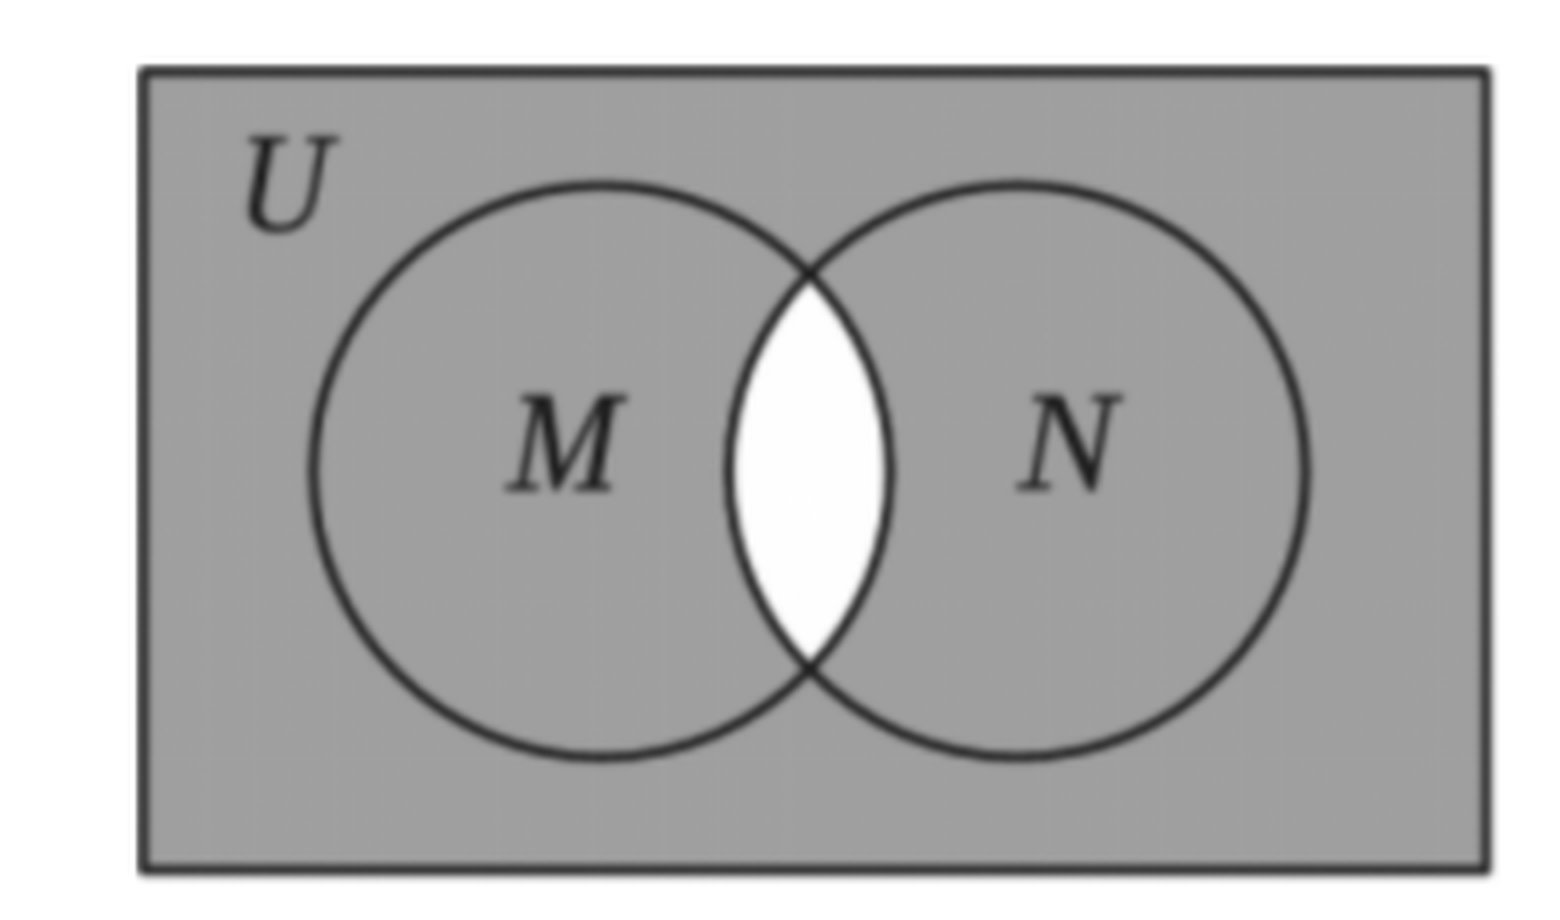
\includegraphics[width=0.40\textwidth]{figures/gao145_q14.png}
\end{center}

\ifanswer
\solbegin
\step{由韦恩图得图中白色区域为集合 $M\cap N$，所以阴影部分表示的集合为 $\overline{M\cap N}$.}
\step{故选 $D$.}
\solend
\fi

% === Q15 ===
\item 已知 $x>-2$，则 $x+\dfrac{1}{x+2}$ 的最小值为\mbox{（\quad）}

\keepwithprev
A. 3\qquad B. 2\qquad C. 1\qquad D. 0

\ifanswer
\solbegin
\step{$x>-2$，则 $x+2>0$，}
\step{所以 $x+\dfrac{1}{x+2}=(x+2)+\dfrac{1}{x+2}-2\geqslant2\sqrt{(x+2)\cdot\dfrac{1}{x+2}}-2=0$，}
\step{当且仅当 $x+2=\dfrac{1}{x+2}$，即 $x=-1$ 时取等号，所以 $x+\dfrac{1}{x+2}$ 的最小值为 $0$.}
\step{故选 $D$.}
\solend
\fi

% 第 16 题：题干在 05 页、解析续至 06 页；两幅数轴标根波浪曲线是【解析】内配图，
% 仅答案版出，放在答案版条件块内 \solbegin 的 \step 之间（照 高一73 第 16 题成例）
\item 关于 $x$ 的不等式 $\dfrac{(x-a)(x-2)^2}{(x-1)(x-5)}\leqslant0$ 的解集中恰有 3 个正整数，则实数 $a$ 的取值范围是\mbox{（\quad）}

\keepwithprev
A. $(-\infty,3]\cup[7,8)$\qquad B. $(-\infty,3)\cup[7,8)$\qquad C. $(-\infty,3]\cup(7,8]$\qquad D. $(-\infty,3)\cup(7,8]$

\ifanswer
\solbegin
\step{由题意，不等式 $\dfrac{(x-a)(x-2)^2}{(x-1)(x-5)}\leqslant0$，}
\step{可化为 $\begin{cases}(x-1)(x-2)^2(x-5)(x-a)\leqslant0\\x\ne1\text{且}x\ne5\end{cases}$，由数轴标根法，}
\step{当 $a=3$ 时，}
\begin{center}
% a=3 数轴标根图取 06 页，去粉色水印、去色、4× LANCZOS 放大；仅答案版出
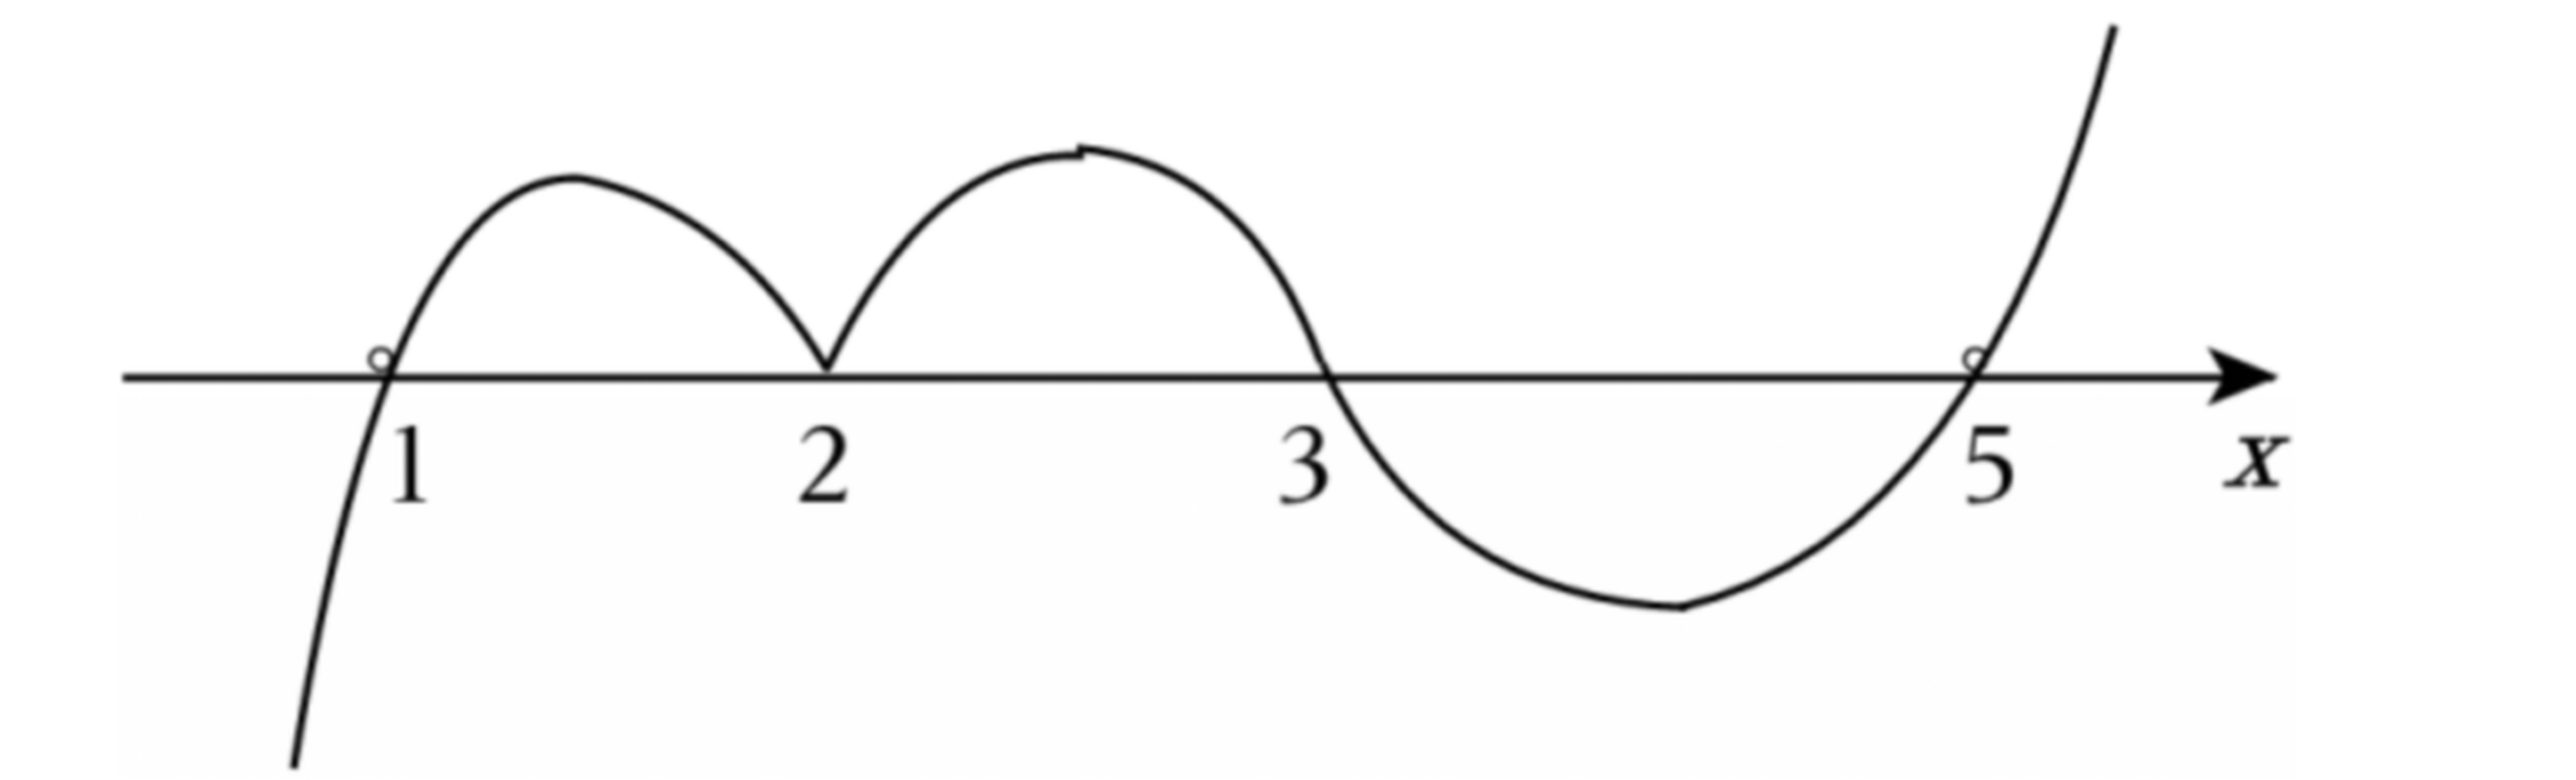
\includegraphics[width=0.62\textwidth]{figures/gao145_q16_a3.png}
\end{center}
\step{得不等式的解集为 $\{x\mid x<1\text{ 或 }x=2\text{ 或 }3\leqslant x<5\}$，}
\step{对应的正整数解为 $2$，$3$，$4$，满足题意，故排除 $B$、$D$；}
\step{当 $a=7$ 时，}
\begin{center}
% a=7 数轴标根图取 06 页，去粉色水印、去色、4× LANCZOS 放大；仅答案版出
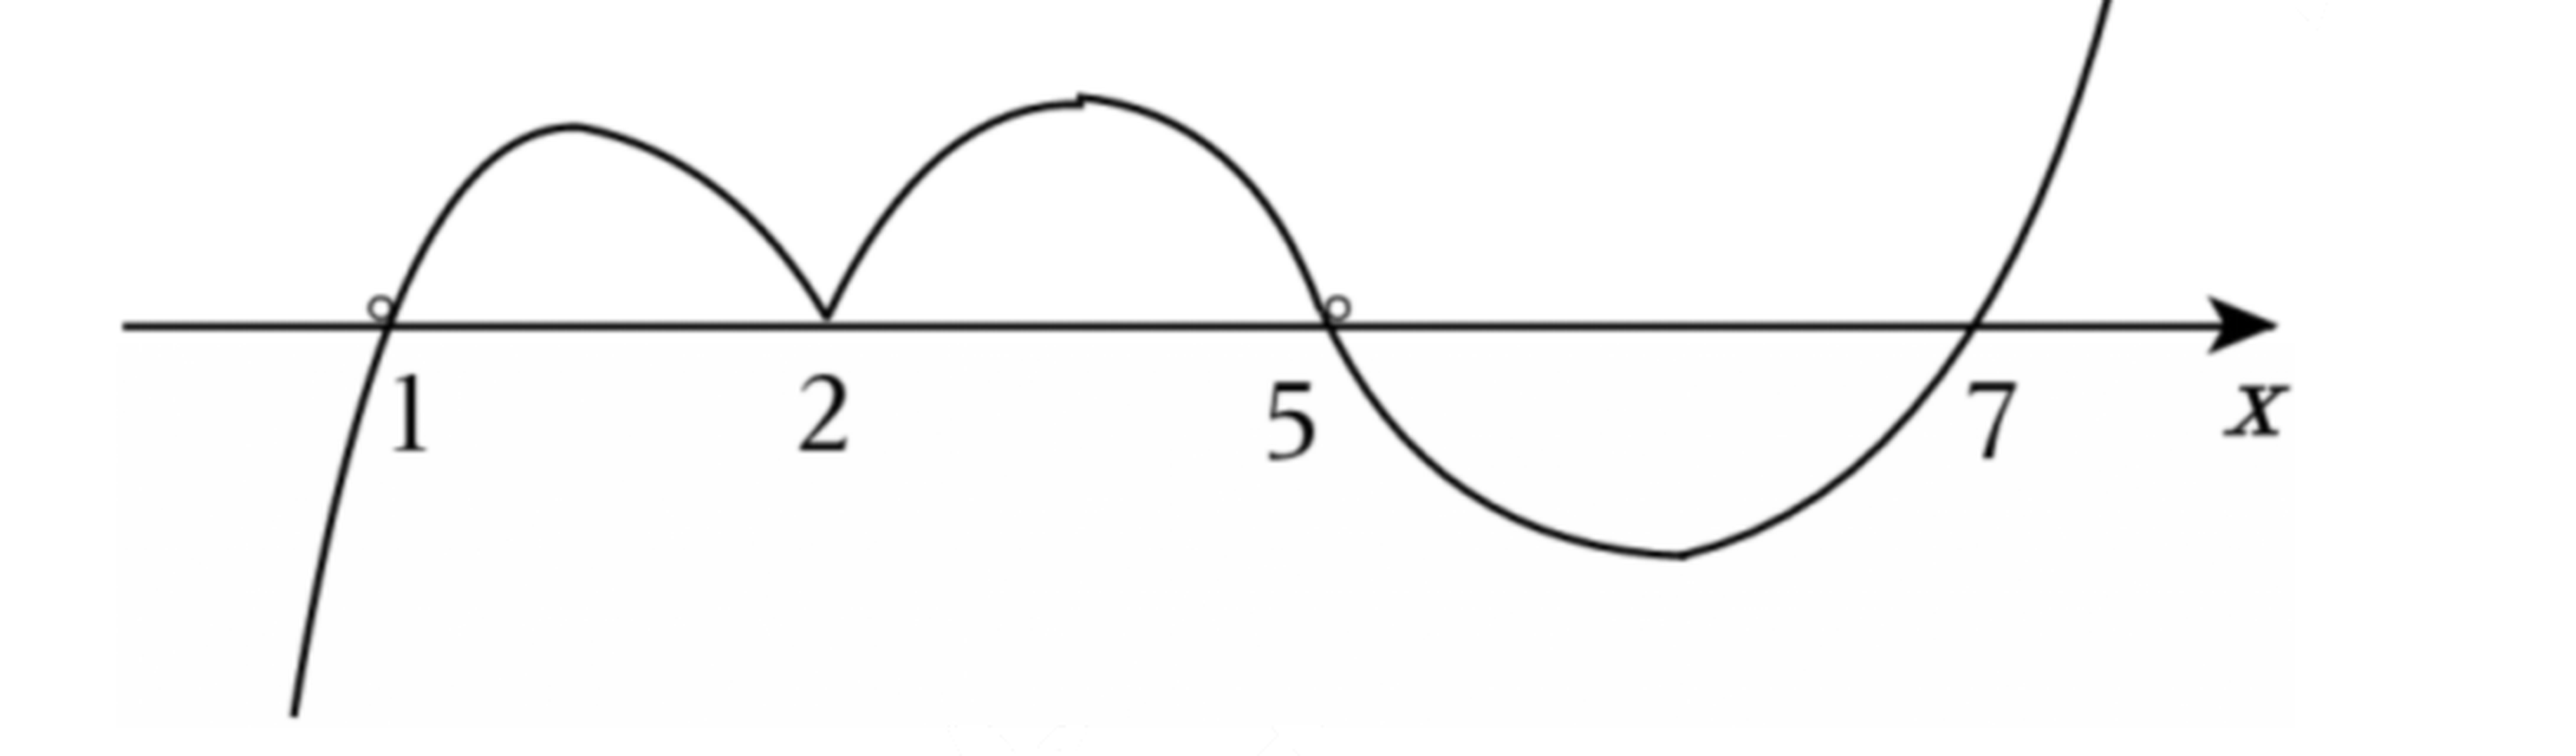
\includegraphics[width=0.62\textwidth]{figures/gao145_q16_a7.png}
\end{center}
\step{得不等式的解集为 $\{x\mid x<1\text{ 或 }x=2\text{ 或 }5<x\leqslant7\}$，}
\step{对应的正整数解为 $2$，$6$，$7$，满足题意，故 $A$ 正确，$C$ 错误.}
\step{故选 $A$.}
\solend
\fi

\end{enumerate}

\bigsec{三、解答题}

\begin{enumerate}
\setcounter{enumi}{16}

% 第 17 题：题干在 06 页、解析续至 07 页，按印刷行断，共 7 行；
% "lg(10÷5)" 的除号照录 \div
\item (1) 已知 $a+a^{-1}=6$，求 $a^2+a^{-2}$ 及 $a^{\frac12}-a^{-\frac12}$ 的值；

(2) 已知 $\lg5=a$，$\lg6=b$，用 $a$、$b$ 分别表示 $\lg2$、$\lg3$、$\lg300$ 和 $\log_{12}15$.

\ifanswer
\solbegin
\step{(1) 因为 $a+a^{-1}=6$，}
\step{所以 $a^2+a^{-2}=(a+a^{-1})^2-2\cdot a\cdot a^{-1}=6^2-2=34$，}
\step{因为 $\left(a^{\frac12}-a^{-\frac12}\right)^2=a-2+a^{-1}=6-2=4$，所以 $a^{\frac12}-a^{-\frac12}=\pm2$；}
\step{(2) $\lg2=\lg(10\div5)=\lg10-\lg5=1-a$，}
\step{$\lg3=\lg(6\div2)=\lg6-\lg2=b-(1-a)=a+b-1$，}
\step{$\lg300=\lg(3\times10^2)=\lg3+\lg10^2=a+b-1+2=a+b+1$，}
\step{所以 $\log_{12}15=\dfrac{\lg15}{\lg12}=\dfrac{\lg3+\lg5}{\lg3+\lg2^2}=\dfrac{a+b-1+a}{a+b-1+2(1-a)}=\dfrac{2a+b-1}{b-a+1}$.}
\solend
\fi

% 第 18 题：题干在 07 页、解析续至 08 页（2 问、分类讨论很长），按印刷行断共 25 行；
% 本卷 Q18 用"图像"（Q13/Q14 用"图象"），逐处照录不统一
\item 已知 $f(x)=(m^2-3m+1)x^{m^2-4m-1}$，$y=f(x)$ 为幂函数且在 $(0,+\infty)$ 上是严格减函数.

(1) 求实数 $m$ 的值以及相应的函数表达式；

(2) 若 $y=f(x)$ 的图像关于 $y$ 轴对称，解关于 $x$ 的不等式 $(x+2)^{1-m}<(3x-1)^{1-m}$.

\ifanswer
\solbegin
\step{(1) 由幂函数的定义得 $m^2-3m+1=1$，}
\step{整理得 $m^2-3m=0$，解得 $m=0$ 或 $m=3$，}
\step{由于 $y=f(x)$ 在 $(0,+\infty)$ 上为严格减函数，}
\step{因此幂函数的指数需满足 $m^2-4m-1<0$，}
\step{当 $m=3$ 时，指数为 $3^2-4\times3-1=-4<0$，满足严格递减条件，}
\step{此时函数表达式为 $f(x)=x^{-4}$，}
\step{当 $m=0$ 时，指数为 $0^2-4\times0-1=-1<0$，满足严格递减条件，}
\step{此时函数表达式为 $f(x)=x^{-1}$，}
\step{所以满足条件的实数 $m$ 为 $0$ 或 $3$，}
\step{对应的函数表达式分别为 $f(x)=x^{-1}$、$f(x)=x^{-4}$；}
\step{(2) 函数图像关于 $y$ 轴对称即函数为偶函数，}
\step{对于 $f(x)=x^{-1}=\dfrac1x$，定义域为 $(-\infty,0)\cup(0,+\infty)$，}
\step{满足 $f(-x)=-f(x)$，为奇函数，图像关于原点对称，}
\step{不满足关于 $y$ 轴对称的条件；}
\step{对于 $f(x)=x^{-4}=\dfrac{1}{x^4}$，定义域为 $(-\infty,0)\cup(0,+\infty)$，}
\step{满足 $f(-x)=f(x)$，为偶函数，图像关于 $y$ 轴对称，}
\step{因此符合条件的 $m$ 值为 $3$，}
\step{将 $m=3$ 代入关于 $x$ 的不等式 $(x+2)^{1-m}<(3x-1)^{1-m}$，}
\step{得 $(x+2)^{1-3}<(3x-1)^{1-3}$，即 $(x+2)^{-2}<(3x-1)^{-2}$，}
\step{因为负指数幂的底数不能为 $0$，所以 $x+2\ne0$ 且 $3x-1\ne0$，}
\step{即 $x\ne-2$ 且 $x\ne\dfrac13$，}
\step{不等式可变形为 $\dfrac{1}{(x+2)^2}<\dfrac{1}{(3x-1)^2}$，}
\step{整理得 $(3x-1)^2<(x+2)^2$，即 $8x^2-10x-3<0$，}
\step{解得 $-\dfrac14<x<\dfrac32$，又 $x\ne-2$ 且 $x\ne\dfrac13$，}
\step{所以不等式的解集为 $\left(-\dfrac14,\dfrac13\right)\cup\left(\dfrac13,\dfrac32\right)$.}
\solend
\fi

% 第 19 题：题干在 08 页、解析续至 09 页，按印刷行断，共 14 行；
% 判别式 cases 块内"△=4a²−16a<0"原卷印扁等边三角 \triangle
%（放大 09 页 zz09_delta.png 与 Q12 高 \Delta 并排确认），逐处照录不统一
\item 已知 $f(x)=ax^2+2ax+4$，$a\in\R$.

(1) 若关于 $x$ 的不等式 $f(x)>0$ 在实数集 $\R$ 上恒成立，求实数 $a$ 的取值范围；

(2) 当 $a<0$ 时，解关于 $x$ 的不等式 $f(x)>(a+1)x+5$.

\ifanswer
\solbegin
\step{(1) 由题意得，关于 $x$ 的不等式 $f(x)>0$ 在实数集 $\R$ 上恒成立，}
\step{即 $ax^2+2ax+4>0$ 在实数集 $\R$ 上恒成立，}
\step{当 $a=0$ 时，不等式为 $4>0$ 恒成立，符合题意；}
\step{当 $a\ne0$ 时，则 $\begin{cases}a>0\\\triangle=4a^2-16a<0\end{cases}$，解得 $0<a<4$.}% 判别式原卷印扁等边三角 $\triangle$，照录
\step{综上所述，实数 $a$ 的取值范围为 $[0,4)$.}
\step{(2) $f(x)=ax^2+2ax+4$，}
\step{当 $a<0$ 时，不等式 $f(x)>(a+1)x+5$ 即为 $ax^2+(a-1)x-1>0$，}
\step{即 $(ax-1)(x+1)>0$，即 $\left(x-\dfrac1a\right)(x+1)<0$，}
\step{当 $a<-1$，即 $\dfrac1a>-1$ 时，解得 $-1<x<\dfrac1a$；}
\step{当 $a=-1$，即 $\dfrac1a=-1$ 时，解得 $x\in\varnothing$；}
\step{当 $-1<a<0$，即 $\dfrac1a<-1$ 时，解得 $\dfrac1a<x<-1$.}
\step{综上所述，当 $a<-1$ 时，不等式的解集为 $\left\{x\mid -1<x<\dfrac1a\right\}$；}
\step{当 $a=-1$ 时，不等式的解集为 $\varnothing$；}
\step{当 $-1<a<0$ 时，不等式的解集为 $\left\{x\mid \dfrac1a<x<-1\right\}$.}
\solend
\fi

% 第 20 题：菜园靠墙图为题目配图（三版都出），题干写"如图"；
% 题干在 09 页（含图）、解析续至 10 页，按印刷行断，共 13 行
\needvspace{8cm}
\item 如图，某人计划用篱笆围成一个一边靠墙（墙足够长）的矩形菜园. 设菜园的长为 $x$ 米，宽为 $y$ 米.

\begin{center}
% 矩形菜园靠墙图取 09 页右下，去粉色水印、去色、4× LANCZOS 放大
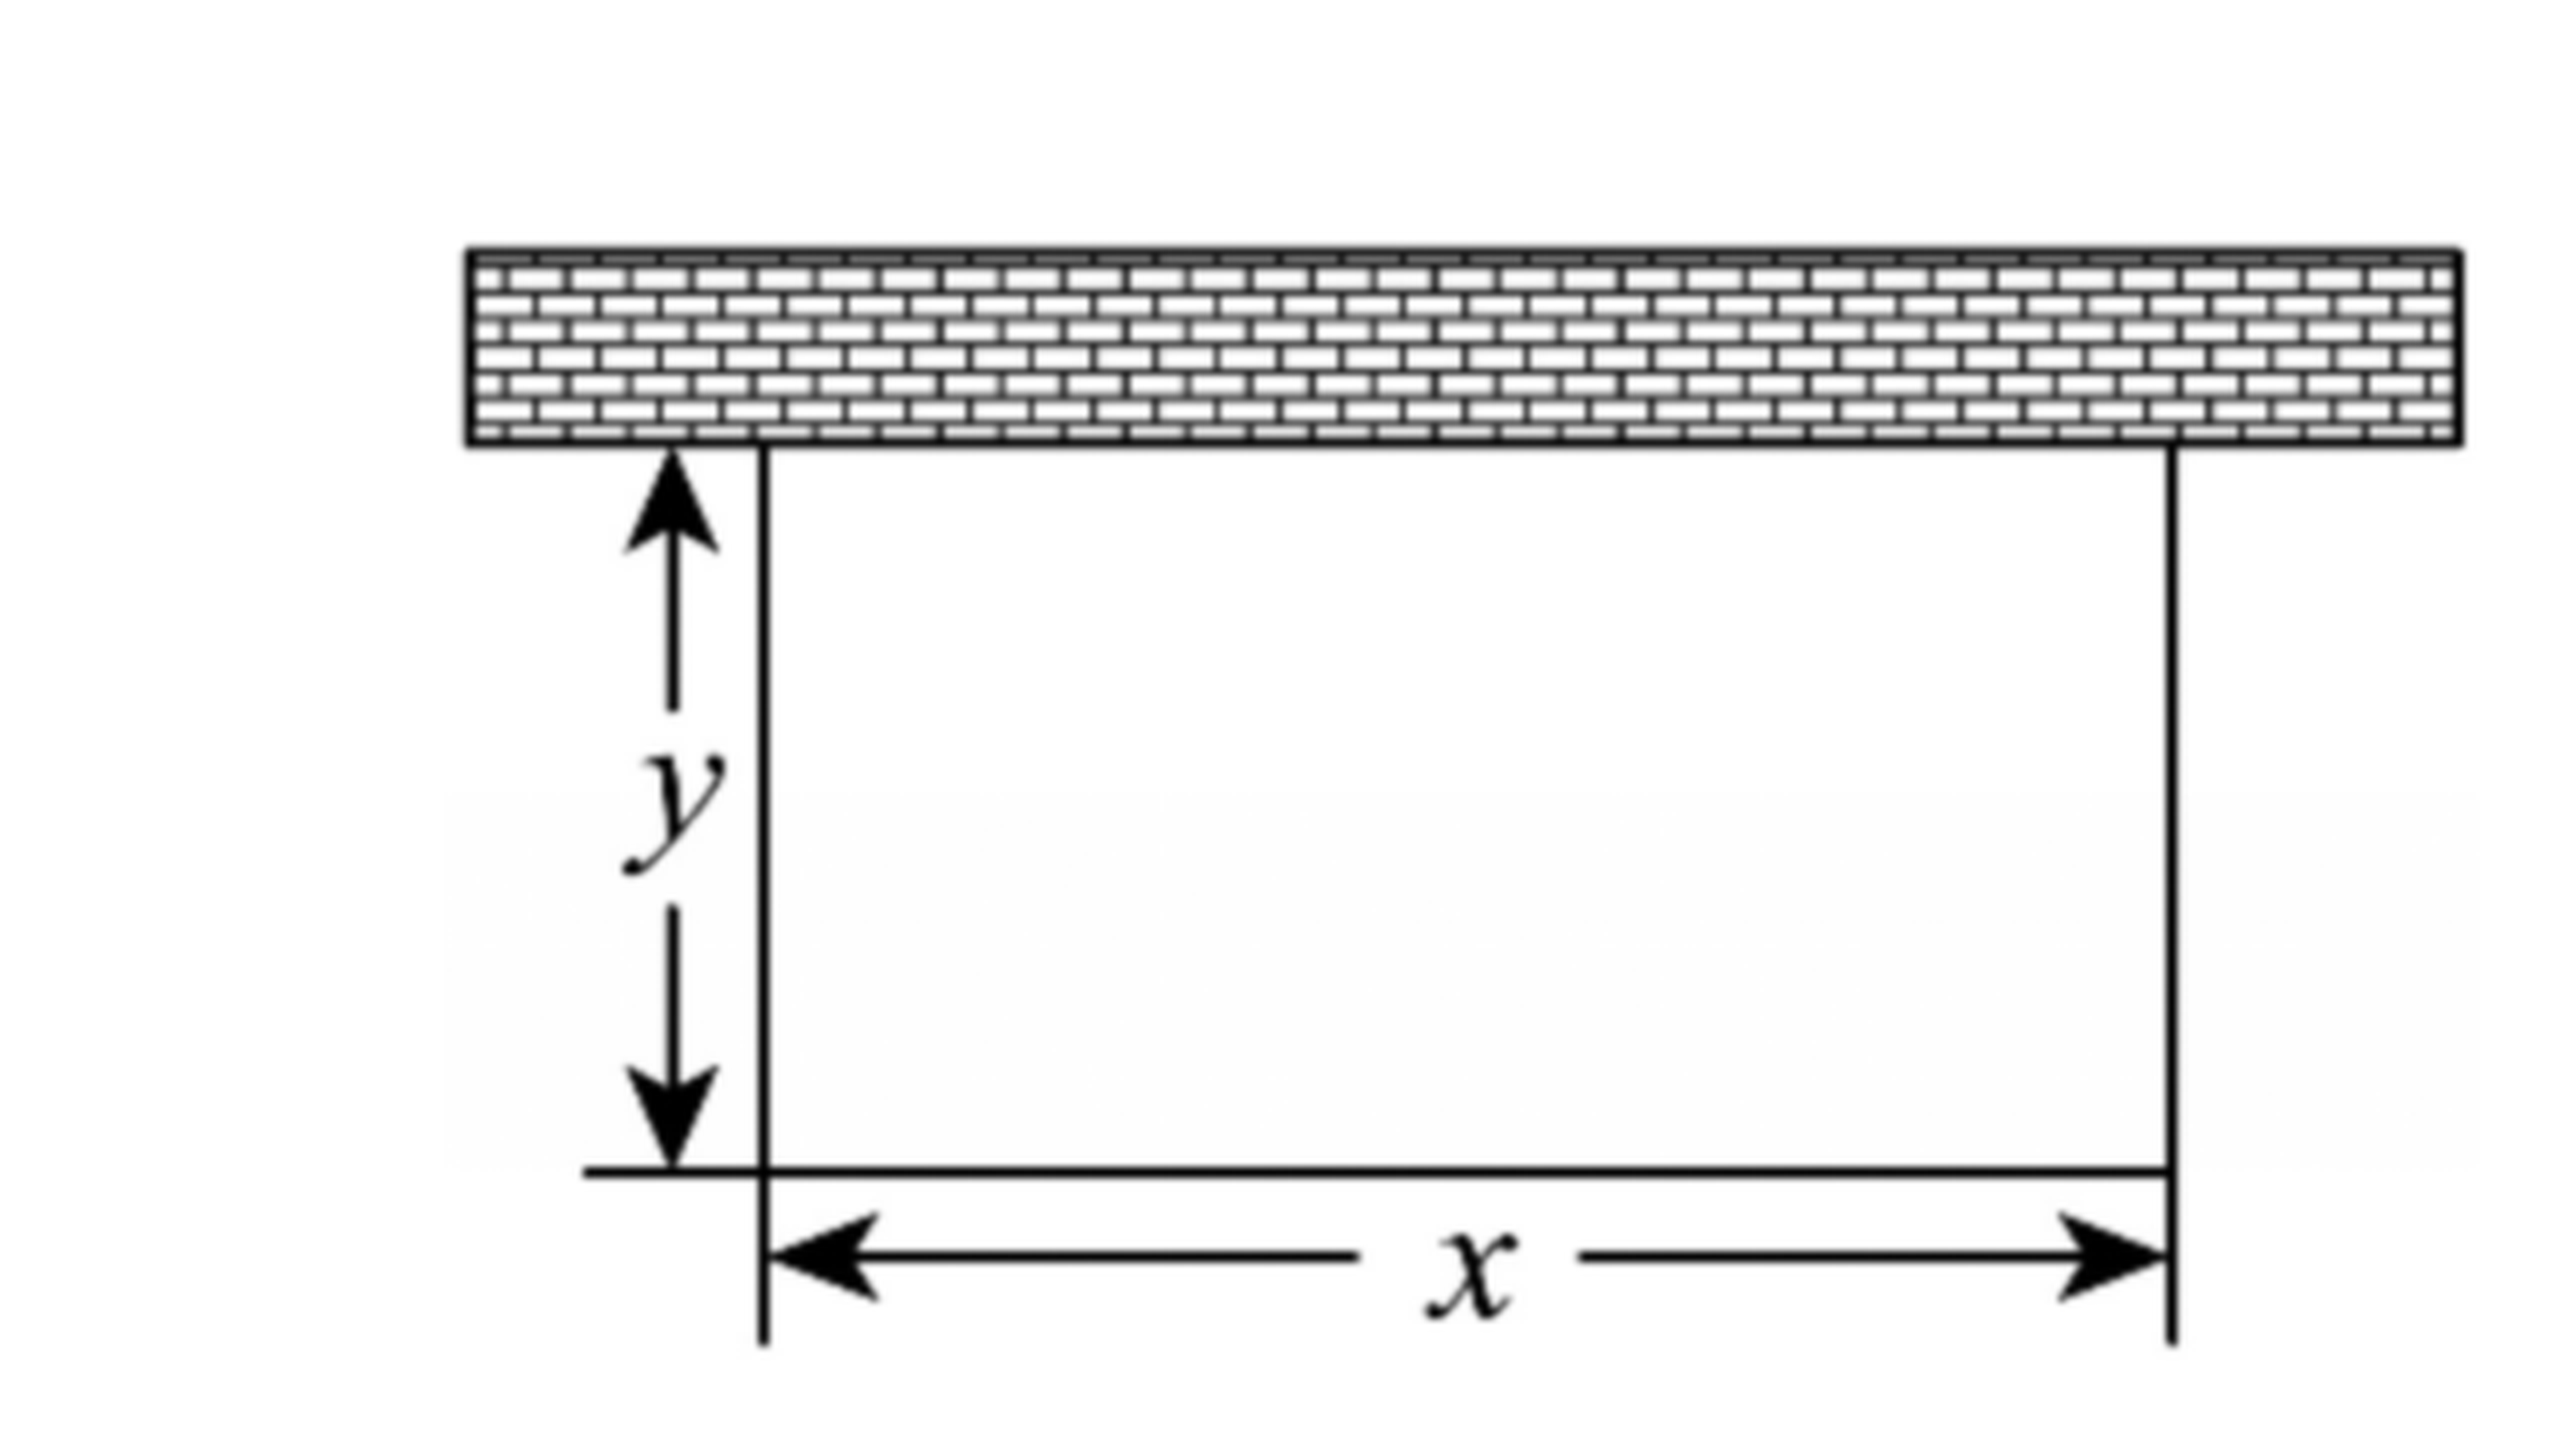
\includegraphics[width=0.55\textwidth]{figures/gao145_q20.png}
\end{center}

(1) 若菜园面积为 72 平方米，则 $x$、$y$ 为何值时，所用篱笆总长最小？

(2) 若 $x$、$y$ 满足 $x+y-xy+63=0$，则菜园面积最小为多少平方米？

\ifanswer
\solbegin
\step{(1) 由题意得，菜园的面积 $S=xy=72$，且 $x>0$，$y>0$，}
\step{所用篱笆总长 $L=x+2y$，}
\step{由基本不等式得 $x+2y\geqslant2\sqrt{x\cdot2y}=2\sqrt{2xy}=2\sqrt{2\times72}=24$，}
\step{当且仅当 $x=2y$ 时取等号，}
\step{联立 $\begin{cases}xy=72\\x=2y\end{cases}$，解得 $\begin{cases}x=12\\y=6\end{cases}$，}
\step{所以当 $x=12$，$y=6$ 时，所用篱笆总长最小；}
\step{(2) 由题意得 $x>0$，$y>0$，且满足 $x+y-xy+63=0$，即 $x+y=xy-63$，}
\step{由基本不等式得 $x+y\geqslant2\sqrt{xy}$，当且仅当 $x=y$ 时取等号，}
\step{所以 $xy-63\geqslant2\sqrt{xy}$. 令 $t=\sqrt{xy}(t>0)$，则 $xy=t^2$，}
\step{上述不等式可化为 $t^2-2t-63\geqslant0$，即 $(t-9)(t+7)\geqslant0$，}
\step{因为 $t>0$，所以 $t+7>0$，故 $t-9\geqslant0$，解得 $t\geqslant9$，所以 $\sqrt{xy}\geqslant9$，}
\step{即 $xy\geqslant81$，当且仅当 $x=y=9$ 时取等号，此时满足 $9+9-81+63=0$，}
\step{所以菜园面积最小为 81 平方米.}
\solend
\fi

% 第 21 题：题干在 10 页、解析续至 11 页（3 问、分类讨论很长），按印刷行断共 22 行；
% 末行"故第 2026 个元素是 2700 之后第一个属于 A 的数，即 2701." 为全卷收尾，
% 无 Q22/Q23、无附加题节；数集 Z/N* 按全稿惯例改 \Z/\N^*
\item 已知集合 $A=\{x\mid x=m^2-n^2$，$m$、$n\in\Z\}$.

(1) 求证：任何奇数 $2k+1(k\in\Z)$ 都是集合 $A$ 中的元素；

(2) 判断偶数 $4k-2(k\in\Z)$ 是否为集合 $A$ 的元素？请说明理由；

(3) 若将集合 $A$ 中的正整数由小到大排列，求出集合 $A$ 中第 2026 个正整数.

\ifanswer
\solbegin
\step{(1) 因为 $x=(k+1)^2-k^2=2k+1(k\in\Z)$，}
\step{所以任何奇数 $2k+1(k\in\Z)$ 都属于集合 $A$；}
\step{(2) 偶数 $4k-2(k\in\Z)$ 不是集合 $A$ 的元素，理由如下：}
\step{由题意得 $x=m^2-n^2=(m-n)(m+n)$，}
\step{当 $m$、$n$ 均为奇数时，设 $m=2k_1+1$，$n=2k_2+1(k_1$、$k_2\in\Z)$，}
\step{则 $m^2-n^2=(2k_1+1)^2-(2k_2+1)^2=(2k_1-2k_2)(2k_1+2k_2+2)$}
\step{$=4(k_1-k_2)(k_1+k_2+1)$，}
\step{因为 $k_1$、$k_2\in\Z$，所以 $k_1-k_2\in\Z$，$k_1+k_2+1\in\Z$，}
\step{从而 $m^2-n^2$ 为 $4$ 的倍数；}
\step{当 $m$、$n$ 均为偶数时，设 $m=2k_1$，$n=2k_2(k_1$、$k_2\in\Z)$，}
\step{$m^2-n^2=4k_1^2-4k_2^2=4(k_1^2-k_2^2)$ 为 $4$ 的倍数；}
\step{当 $m$、$n$ 为一个偶数一个奇数时，不妨设 $m$ 为偶数，$n$ 为奇数，}
\step{设 $m=2k_1$，$n=2k_2+1(k_1$、$k_2\in\Z)$，}
\step{则 $m^2-n^2=4k_1^2-(2k_2+1)^2=4(k_1^2-k_2^2-k_2)-1$ 为奇数.}
\step{无论哪种情况均不满足 $4k-2(k\in\Z)$，}
\step{故偶数 $4k-2(k\in\Z)$ 不是集合 $A$ 的元素；}
\step{(3) 由前两问得，$4$ 的倍数和奇数属于集合 $A$ 中的元素，}
\step{令集合 $A$ 中的正整数元素为 $4k-3$、$4k-1$、$4k(k\in\N^*)$，}
\step{对任意的 $k\in\N^*$，连续的 $4$ 个整数 $4k-3$、$4k-2$、$4k-1$、$4k$ 中}
\step{有三个数 $4k-3$、$4k-1$、$4k$ 都在集合 $A$ 中，}
\step{因为 $2026=3\times675+1$，所以集合 $A$ 中第 $2025$ 个元素为 $4\times675=2700$，}
\step{故第 2026 个元素是 2700 之后第一个属于 $A$ 的数，即 2701.}
\solend
\fi

\end{enumerate}

\end{document}
"
% 紧凑版：xelatex "\def\iscompact{1}% 高一145_市二中学_期中.tex
%   —— 高一上数学"2026-2027 年市二中学高一上期中"（试卷版/答案版/紧凑版）
% 试卷版：xelatex 高一145_市二中学_期中.tex
% 答案版：xelatex "\def\isanswer{1}% 高一145_市二中学_期中.tex
%   —— 高一上数学"2026-2027 年市二中学高一上期中"（试卷版/答案版/紧凑版）
% 试卷版：xelatex 高一145_市二中学_期中.tex
% 答案版：xelatex "\def\isanswer{1}\input{高一145_市二中学_期中.tex}"
% 紧凑版：xelatex "\def\iscompact{1}\input{高一145_市二中学_期中.tex}"
%
% ① 原始材料：微信公众号"魔都数学加油站"文章，连载"27学年高一145"，原文标题
% "27学年高一145——2026-2027年上海市市二中学高一上期中"；
% 原文链接：https://mp.weixin.qq.com/s/6V-i9KE0GWodC-wmd5z8nQ 。
% 正文为 11 张 PNG 页（01/02/03/08/10/11 为 4762×6735，04/05/06/07/09 为 2560×3620，
% 同一篇各页分辨率不同，逐页按各自分辨率裁图核对，别按预览比例换算裁框）。
% 题目下印【答案】或【解析】，为混合体例讲评版：Q3 只印【答案】、无【解析】，其余
% 18 题印【解析】。题目、解析均据原图转录；卷面粉红色水印"魔都数学加油站"及
% 公众号页脚未录入。
% 全卷插图情况（逐页通读 11 页确认，题干写"如图"处均配有图）：
%   · Q14 韦恩图（05 页右侧，全集 U 矩形＋两圆 M/N＋白色交集、灰色阴影＋U/M/N 标注）：
%     题目配图（选择题选项旁），三版都出，裁自 05 页去水印去色 4× 放大存
%     figures/gao145_q14.png；
%   · Q16 两幅数轴标根波浪曲线（06 页，a=3 与 a=7 各一幅，标根法画
%     (x-1)(x-2)^2(x-5)(x-a)≤0 的符号曲线）：【解析】内的配图，仅答案版出，
%     裁 figures/gao145_q16_a3.png / figures/gao145_q16_a7.png（或合并一张），
%     放在答案版条件块内 \solbegin 的 \step 之间（照 高一73 第 16 题成例）；
%   · Q20 矩形菜园靠墙图（09 页右下，灰色砖墙＋矩形菜园＋x/y 标注＋箭头）：
%     题目配图，三版都出，裁自 09 页去水印去色 4× 放大存 figures/gao145_q20.png；
%   其余各页逐页确认无其它题目配图、无表格、亦无"题干写如图而源码漏图"一处。
%
% 卷首标题：原卷印作"2026-2027 年市二中学高一上期中"，年份区间按全稿惯例排 en dash；
% 原卷卷面未印副标题，本稿按同期中卷（高一140／141／143／144）知识模块口径补出
% "集合与常用逻辑用语、不等式、函数"。
%
% 题号体例：本卷共 19 题——一、填空题 3—12（10 题）、二、选择题 13—16（4 题）、
% 三、解答题 17—21（5 题）。三节分别 \setcounter{enumi}{2}／{12}／{16}。
% 原卷从第 3 题起、无第 1、2 题，本稿保留原题号；全卷无附加题节。
%
% ② 与原卷的排版差异：
%   ① 原文从第 3 题起，本稿保留原题号；共 19 题三节；
%   ② 混合体例：原卷 Q3 只印【答案】、无【解析】（"第一步应假设___。
%      【答案】x≤2 或 y≤2"），按 高一140 第 5 题成例提 \ans{}、不补造解析；
%      其余 18 题印【解析】，用 \solbegin…\solend，选择题答案在解析末句"故选 X"
%      （Q13 选 B、Q14 选 D、Q15 选 D、Q16 选 A，逐个放大原图核实）、
%      题干括号 \mbox{（\quad）} 留空、不另提 \ans{}；填空／解答答案落在解析里；
%      答案版【答案】/【解析】标记数 = 19（1 个 \ans ＋ 18 个 \solbegin）= 全卷题数；
%   ③ 原卷卷面未印副标题，本稿按知识模块口径补出；
%   ④ 原卷填空横线按全稿惯例排 \blankline[4.4em]；选择题括号排 \mbox{（\quad）}、
%      选项段前按惯例加 \keepwithprev；解答题不留作答区、不加 \anspace
%      （原卷为讲评版，与 129／131／132／133／136／140／141／143／144 同）；
%   ⑤ 数集：Q9"a、b∈R"、Q12"a∈R"、Q21"m、n∈Z""k∈Z""k∈N*"等原卷印
%      斜体或黑板粗体 R/Z/N，按全稿惯例统一改 \R／\Z／\N^*；绝对值排 \lvert…\rvert，
%      集合描述竖线排 \mid；不等号按全稿惯例排 \leqslant／\geqslant；
%      补集照原卷上划线排 \overline{M}／\overline{N}（Q14 选项 B/C/D 逐处核）；
%      空集记号 \varnothing；\subset（单线⊂）与 \subseteq（带下划线⊆）逐处照录不统一；
%   ⑥ 子题标号 (1)(2)(3) 原卷印半角括号照录；圈数字进数学式用 \text{①}（否则 FONTCHK 挂）；
%      \left…\right 不得拆到不同 $…$ 组；cases 块整体算一个印刷行；
%   ⑦ 题干／解析中的中文弯引号按原卷照录（Q3"若 x+y>4，则 x>2 且 y>2"、
%      Q11"a₁/a₂=b₁/b₂""M=N"、选填"充分非必要""必要非充分""充要""既非充分也非必要"
%      等，含引号内空格），注释内一律 ASCII 引号；数学式内 CJK 用 \text{}；
%   ⑧ 半角逗号在数学组之间是全稿惯例、非笔误（如 Q5"x₁+x₂=6，x₁x₂=√3"、
%      Q7"a>1，b>1"、指数／对数式内逗号），逐处照录别改全角；行末西文句点照录为
%      ASCII `.`；行中全角逗号／顿号照录；
%   ⑨ "图像／图象"逐处照录不统一（Q18"图像关于 y 轴对称"等，核全卷）；
%   ⑩ 判别式 Δ/△ 混用是照录项：Q12 解析"Δ=a²−4a²(2a−3)>0"、
%      Q19 解析"Δ=4a²−16a<0"等，放大原图判断是高 \Delta（等腰偏高、高>宽）
%      还是扁 \triangle，逐处照录不得统一（参照 高一142／144 头注④口径）；
%   ⑪ 一条 \step = 原卷解析的一个印刷行，cases 块整体算一个印刷行；别把原卷折行
%      并起来、别把一行拆多条。Q6 分段讨论、Q12 三个 cases 条件组、Q16 数轴标根、
%      Q18／Q19 分类讨论、Q21 三问均按印刷行逐条断，不丢行；
%   ⑫ Q14 韦恩图为"题干＋选项＋图"整块，加 \needvspace 守卫推走（守卫放 \item 之前，
%      见 高一140 Q14、高一144 Q17 成例与切页审计 B 类坑）；Q20 菜园图同理；
%      三版切页审计均"合计异常：无"；
%   ⑬ 跨页续印按题合并：Q3/4/5/6 在 01 页（Q6 解析续 02 页顶）；Q7/8/9/10 在 02 页
%      （Q10 解析续 03 页）；Q11/12 在 03 页（Q12 解析续 04 页，很长）；
%      Q13 在 04 页末、解析在 05 页顶；Q14/15/16 在 05 页（Q16 解析续 06 页含两幅数轴图）；
%      Q17 在 06 页、解析续 07 页；Q18 在 07 页、解析续 08 页；Q19 在 08 页、解析续 09 页；
%      Q20 在 09 页（含菜园图）、解析续 10 页；Q21 在 10 页、解析续 11 页
%      （末页收尾"故第 2026 个元素是 2700 之后第一个属于 A 的数，即 2701."、
%      无 Q22/Q23、无附加题节）。本稿按题连排，不丢行、不并折行；
%   ⑭ 原卷解析内若有红色"法一／法二"之类小标题，按全稿惯例排 \stepm{标签}{…}
%      （黑体着色、不引入红色、不改 common.sty），头注注明；水印"魔都数学加油站"
%      红色不录入。
%
% ③ 行数复核：一条 \step／\stepm = 原卷解析的一个印刷行，cases 块作一个印刷行计。
%   逐题数（主会话逐页核对定稿）：Q3：0（只印【答案】、提 \ans{}，不计入 \step 账）；
%   Q4：3；Q5：2；Q6：10；Q7：3；Q8：3；Q9：2；Q10：7；Q11：4；Q12：12；
%   Q13：2；Q14：2；Q15：4；Q16：9；Q17：7；Q18：25；Q19：14；Q20：13；Q21：22。
%   合计 144 条 \step（本卷无 \stepm：解析内无红色"法一／法二"类小标题），
%   与原卷逐题印刷行相等。全卷 18 题设 \solbegin…\solend ＋ Q3 一处 \ans{}，
%   答案版【答案】/【解析】标记数 = 19 = 全卷题数。
%
% ④ 判别式／子集符号结论（逐处放大原图照录、不得统一，主会话像素级复核）：
%   判别式全卷 2 处、两形混用逐处照录不统一（参照 高一142／144 头注④口径）：
%     · Q12 解析 cases 块"Δ=a²−4a²(2a−3)>0" 原卷印等腰偏高粗三角（高>宽），
%       照录 \Delta（放大 04 页 /tmp/gao145s2/main_q12_delta.png 确认）；
%     · Q19 解析 cases 块"△=4a²−16a<0" 原卷印扁等边空心三角（宽≈高、细线），
%       照录 \triangle（放大 09 页 /tmp/gao145s2/main_q19_delta.png 确认）。
%   子集／补集：Q14 选项 A `M\cup N`、B `M\cap\overline{N}`（上划线只在 N 上）、
%   C `\overline{M\cup N}`（罩整个 M∪N）、D `\overline{M\cap N}`（罩整个 M∩N，
%   非 \overline{M}\cap N；放大 05 页 /tmp/gao145s2/main_q14_opts.png 确认），
%   阴影为灰色区域＝全集减白色交集，答案 D，照录 \overline{M\cap N}；
%   全集卷无 \subset／\subseteq 混用（本卷集合题用 \cup／\cap／\overline{}）；
%   空集 \varnothing（Q19 解析 x∈\varnothing）；数集 \R／\Z／\N^* 归一见 ② ⑤。
%
% ⑤ 存疑照录（放大原图确认，照录未改、正文对应处另有 % 注）：
%   1. Q3 题干"若 x+y>4，则 x>2 且 y>2" 后"时"前留一空格、弯引号内空格照录；
%      该卷混合体例（Q3 只印【答案】、提 \ans{}）见 ② ②。
%   2. Q4／Q5 解析中的"1，3，5 和 6"、"x₁+x₂=6,x₁x₂=√3" 等半角／全角逗号
%      逐处照原卷（放大 01 页确认），数学式内半角逗号为全稿惯例、非笔误。
%   3. Q14 选项 D 上划线罩住整个 M∩N（而非仅罩 M），照录 \overline{M\cap N}。
%   4. Q12 判别式高 \Delta 与 Q19 判别式扁 \triangle 两形混用，逐处照录不统一（见 ④）。
%   全卷除此 4 类外未发现其它笔误／自相矛盾处。
%
% ⑥ 跨页续印按题合并说明：见 ② ⑬。
%
\documentclass[a4paper,11pt]{article}
\usepackage{common}

\begin{document}

\examtitlest[3]{2026--2027 年市二中学高一上期中}{集合与常用逻辑用语、不等式、函数}

\bigsec{一、填空题}

\begin{enumerate}
\setcounter{enumi}{2}

% 第 3 题：原卷只印【答案】、无【解析】（放大 01 页确认），按 高一140 第 5 题成例
% 提 \ans{}、不补造解析；题干中文弯引号与"时"前空格照录
\item 用反证法证明命题：“若 $x+y>4$，则 $x>2$ 且 $y>2$” 时，第一步应假设\blankline[4.4em].

\ifanswer
\ans{$x\leqslant2$ 或 $y\leqslant2$}
\fi

% === Q4 ===
\item 设集合 $M$ 满足 $\{1,3,5,6\}\cup M=\{1,2,3,4,5,6\}$，则满足条件的所有 $M$ 的个数为\blankline[4.4em].

\ifanswer
\solbegin
\step{集合 $M$ 满足 $\{1,3,5,6\}\cup M=\{1,2,3,4,5,6\}$，}
\step{则 $M$ 中必含有 $2$ 和 $4$，$1$，$3$，$5$ 和 $6$ 可以选也可不选，}
\step{则满足条件的所有 $M$ 的数目相当于集合 $\{1,3,5,6\}$ 的子集的个数 $2^4=16$.}
\solend
\fi

% === Q5 ===
\item 已知方程 $x^2-6x+\sqrt3=0$ 的两根为 $x_1$ 和 $x_2$，则 $(x_1-x_2)^2=$\blankline[4.4em].

\ifanswer
\solbegin
\step{因为方程 $x^2-6x+\sqrt3=0$ 的两根为 $x_1$ 和 $x_2$，所以 $x_1+x_2=6,x_1x_2=\sqrt3$，}% 数学式内半角逗号为全稿惯例，照录
\step{所以 $(x_1-x_2)^2=(x_1+x_2)^2-4x_1x_2=36-4\sqrt3$.}
\solend
\fi

% 第 6 题：题干在 01 页，解析续至 02 页顶（末 2 行），按印刷行逐条断，共 10 行
\item 不等式 $\lvert x-2026\rvert+\lvert x-2029\rvert>3$ 的解集是\blankline[4.4em].

\ifanswer
\solbegin
\step{当 $x<2026$ 时，$x-2026<0$，$x-2029<0$，}
\step{原不等式可化为 $(2026-x)+(2029-x)>3$，解得 $x<2026$，}
\step{故此时，不等式的解为 $x<2026$；}
\step{当 $2026\leqslant x\leqslant2029$ 时，$x-2026\geqslant0$，$x-2029\leqslant0$，}
\step{原不等式可化为 $(x-2026)+(2029-x)>3$，即 $3>3$，显然不成立，}
\step{故此时，不等式无解；}
\step{当 $x>2029$ 时，$x-2026>0$，$x-2029>0$，}
\step{原不等式可化为 $(x-2026)+(x-2029)>3$，解得 $x>2029$，}
\step{故此时，不等式的解为 $x>2029$.}
\step{综上，原不等式的解集为 $(-\infty,2026)\cup(2029,+\infty)$.}
\solend
\fi

% === Q7 ===
\item 已知 $a>1$，$b>1$，若 $\log_a b+\log_b a=2$，且 $ab=2$，则 $\log_2(a+b)=$\blankline[4.4em].

\ifanswer
\solbegin
\step{由 $\log_a b+\log_b a=2$，$a>1$，$b>1$，得 $\log_a b+\dfrac{1}{\log_a b}=2$，}
\step{即 $(\log_a b)^2-2\log_a b+1=0$，则 $(\log_a b-1)^2=0$，解得 $\log_a b=1$，即 $a=b$，}
\step{又 $ab=2$，所以 $a=b=\sqrt2$，所以 $\log_2(a+b)=\log_2 2\sqrt2=\log_2 2^{\frac32}=\dfrac32$.}
\solend
\fi

% === Q8 ===
\item 已知 $m>0$，$n>0$，且 $m+n=1$，则 $\dfrac1m+\dfrac4n$ 的最小值为\blankline[4.4em].

\ifanswer
\solbegin
\step{由 $m>0$，$n>0$，$m+n=1$，}
\step{则 $\dfrac1m+\dfrac4n=(m+n)\left(\dfrac1m+\dfrac4n\right)=5+\dfrac nm+\dfrac{4m}n\geqslant5+2\sqrt{\dfrac nm\cdot\dfrac{4m}n}=9$，}
\step{当且仅当 $n=2m=\dfrac23$ 时，上式取得等号，故最小值为 $9$.}
\solend
\fi

% === Q9 ===
\item 已知 $a$、$b\in\R$，且 $3a+2b=1$，则 $8^a+4^b$ 最小值为\blankline[4.4em].

\ifanswer
\solbegin
\step{因为 $3a+2b=1$，所以 $8^a+4^b=2^{3a}+2^{2b}\geqslant2\sqrt{2^{3a+2b}}=2\sqrt2$，}
\step{当且仅当 $3a=2b$ 时取等号，故最小值为 $2\sqrt2$.}
\solend
\fi

% 第 10 题：题干在 02 页、解析续至 03 页顶，按印刷行断，共 7 行
\item 已知关于 $x$ 的不等式 $ax^2+bx+c>0$ 的解集为 $\{x\mid 1<x<2\}$，则关于 $x$ 的不等式 $bx^2-ax+c<0$ 的解集为\blankline[4.4em].

\ifanswer
\solbegin
\step{已知关于 $x$ 的不等式 $ax^2+bx+c>0$ 的解集为 $\{x\mid 1<x<2\}$，}
\step{由解集为 $1<x<2$ 且二次函数在两根之间为正，得 $a<0$，两个根为 $1$，$2$，}
\step{所以 $ax^2+bx+c=a(x-1)(x-2)=ax^2-3ax+2a$，}
\step{比较系数得 $b=-3a$，$c=2a$.}
\step{于是 $bx^2-ax+c=-3ax^2-ax+2a=-a(3x-2)(x+1)$，}
\step{$a<0$，故 $bx^2-ax+c<0$ 等价于 $(3x-2)(x+1)<0$，解得 $-1<x<\dfrac23$，}
\step{故 $bx^2-ax+c<0$ 的解集为 $\left\{x\mid -1<x<\dfrac23\right\}$.}
\solend
\fi

% 第 11 题：题干引号内空格照录（放大 03 页确认），四组选填引号亦同；
% 结论"故为必要非充分条件"照录，解析共 4 个印刷行
\item 设 $a_1$、$b_1$、$a_2$、$b_2$ 均为非零实数，不等式 $a_1x+b_1>0$ 和 $a_2x+b_2>0$ 的解集分别为集合 $M$、$N$，那么 “ $\dfrac{a_1}{a_2}=\dfrac{b_1}{b_2}$ ” 是 “ $M=N$ ” 的\blankline[4.4em]条件（选填 “ 充分非必要 ”、“ 必要非充分 ”、“ 充要 ” 和 “ 既非充分也非必要 ”）.

\ifanswer
\solbegin
\step{当 $a_1=b_1=1$，$a_2=b_2=-1$ 时，满足 $\dfrac{a_1}{a_2}=\dfrac{b_1}{b_2}$，}
\step{但是 $M=N$ 不成立，即充分性不成立；}
\step{若 $M=N$ 时，$\dfrac{a_1}{a_2}=\dfrac{b_1}{b_2}$ 一定成立，即必要性成立.}
\step{故为必要非充分条件.}
\solend
\fi

% 第 12 题：题干在 03 页、解析续至 04 页（很长，含 3 个 cases 条件组），
% 按印刷行逐条断共 12 行；cases 块整体算一个印刷行
\item 已知 $f(x)=\dfrac{ax+3}{x-2}$（常数 $a\in\R$）. 函数 $y=f(x)$ 在区间 $[3,+\infty)$ 上是严格减函数，且函数值不恒为负. 若关于 $x$ 的方程 $f(x)=\dfrac{a}{ax-1}$ 有两个不相等的实数根 $x_1$ 和 $x_2$，则 $a$ 的取值范围是\blankline[4.4em].

\ifanswer
\solbegin
\step{$f(x)=\dfrac{ax+3}{x-2}=a+\dfrac{3+2a}{x-2}$，定义域 $(-\infty,2)\cup(2,+\infty)$，}
\step{由于 $y=f(x)$ 在区间 $[3,+\infty)$ 上是严格减函数，且函数值不恒为负，}
\step{所以 $\begin{cases}3+2a>0\\a+\dfrac{3+2a}{3-2}\geqslant0\end{cases}\Rightarrow a\geqslant-1$，}
\step{若关于 $x$ 的方程 $f(x)=\dfrac{a}{ax-1}$ 有两个不相等的实数根 $x_1$ 和 $x_2$，}
\step{则 $\dfrac{ax+3}{x-2}=\dfrac{a}{ax-1}$，即 $(ax+3)(ax-1)=a(x-2)$，$x\ne2$ 且 $ax-1\ne0$，}
\step{当 $a\ne0$ 且 $a\geqslant-1$ 时，$(ax+3)(ax-1)=a(x-2)$，$x\ne2$ 且 $ax-1\ne0$，}
\step{可化为 $\begin{cases}a^2x^2+ax+2a-3=0\\x\ne2,x\ne\dfrac1a\end{cases}$，}
\step{要使方程有两个不相等的实数根 $x_1$ 和 $x_2$，}
\step{则 $\begin{cases}\Delta=a^2-4a^2(2a-3)>0\\a\geqslant-1\text{且}a\ne0\\4a^2+2a+2a-3\ne0\\a^2\cdot\dfrac1{a^2}+a\cdot\dfrac1a+2a-3\ne0\end{cases}\Rightarrow\begin{cases}a<\dfrac{13}{8}\\a\geqslant-1\text{且}a\ne0\\a\ne\dfrac12\text{且}a\ne-\dfrac32\\a\ne\dfrac12\end{cases}$，}% 判别式原卷印等腰偏高三角 $\Delta$，照录（放大 04 页 zz04_delta.png 确认）
\step{得 $-1\leqslant a<\dfrac{13}{8}$ 且 $a\ne0,a\ne\dfrac12$；}
\step{当 $a=0$ 时，方程无解；}
\step{所以 $a$ 的取值范围是 $[-1,0)\cup\left(0,\dfrac12\right)\cup\left(\dfrac12,\dfrac{13}{8}\right)$.}
\solend
\fi

\end{enumerate}

\bigsec{二、选择题}

\begin{enumerate}
\setcounter{enumi}{12}

% 第 13 题：题干在 04 页末、解析在 05 页顶；"图象"照录（本卷 Q13、Q14 用"图象"）
\item 已知幂函数 $f(x)$ 的图象过点 $\left(7,\dfrac{1}{\sqrt7}\right)$，则 $f(x)=$\mbox{（\quad）}

\keepwithprev
A. $x^{-2}$\qquad B. $x^{-\frac12}$\qquad C. $x^{\frac12}$\qquad D. $x^2$

\ifanswer
\solbegin
\step{设幂函数 $f(x)=x^\alpha(\alpha\in\R)$，因为幂函数的图象过点 $\left(7,\dfrac{1}{\sqrt7}\right)$，}
\step{所以 $7^\alpha=\dfrac{1}{\sqrt7}=7^{-\frac12}$，所以 $\alpha=-\dfrac12$，故 $f(x)=x^{-\frac12}$. 故选 $B$.}
\solend
\fi

% 第 14 题：韦恩图为题目配图（三版都出），"题干＋选项＋图"整块，needvspace
% 守卫放在 \item 之前（Q14 为选择题节内第二题，不会让节标题孤落页末）；
% D 选项上划线罩住整个 M∩N（放大 05 页 zz05_q14D.png 确认，非 \overline{M}\cap N）
\needvspace{9cm}
\item 已知全集 $U$ 和集合 $M$、$N$，用集合语言表示图中的阴影部分，正确的是\mbox{（\quad）}

\keepwithprev
A. $M\cup N$\qquad B. $M\cap\overline{N}$\qquad C. $\overline{M\cup N}$\qquad D. $\overline{M\cap N}$

\begin{center}
% 韦恩图取 05 页右侧，去粉色水印、去色、4× LANCZOS 放大
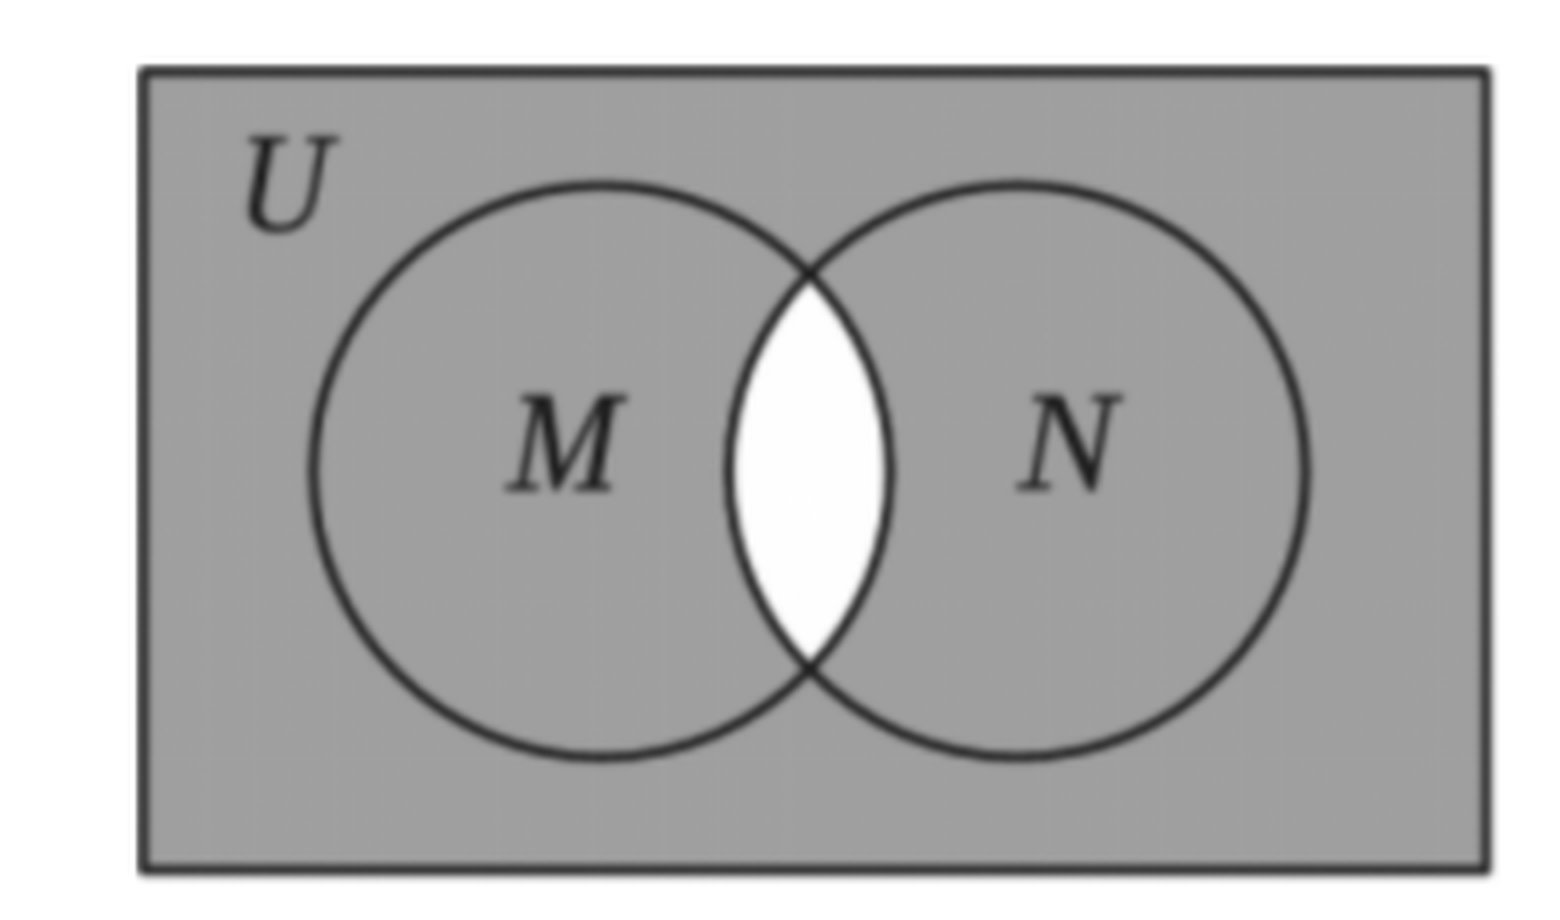
\includegraphics[width=0.40\textwidth]{figures/gao145_q14.png}
\end{center}

\ifanswer
\solbegin
\step{由韦恩图得图中白色区域为集合 $M\cap N$，所以阴影部分表示的集合为 $\overline{M\cap N}$.}
\step{故选 $D$.}
\solend
\fi

% === Q15 ===
\item 已知 $x>-2$，则 $x+\dfrac{1}{x+2}$ 的最小值为\mbox{（\quad）}

\keepwithprev
A. 3\qquad B. 2\qquad C. 1\qquad D. 0

\ifanswer
\solbegin
\step{$x>-2$，则 $x+2>0$，}
\step{所以 $x+\dfrac{1}{x+2}=(x+2)+\dfrac{1}{x+2}-2\geqslant2\sqrt{(x+2)\cdot\dfrac{1}{x+2}}-2=0$，}
\step{当且仅当 $x+2=\dfrac{1}{x+2}$，即 $x=-1$ 时取等号，所以 $x+\dfrac{1}{x+2}$ 的最小值为 $0$.}
\step{故选 $D$.}
\solend
\fi

% 第 16 题：题干在 05 页、解析续至 06 页；两幅数轴标根波浪曲线是【解析】内配图，
% 仅答案版出，放在答案版条件块内 \solbegin 的 \step 之间（照 高一73 第 16 题成例）
\item 关于 $x$ 的不等式 $\dfrac{(x-a)(x-2)^2}{(x-1)(x-5)}\leqslant0$ 的解集中恰有 3 个正整数，则实数 $a$ 的取值范围是\mbox{（\quad）}

\keepwithprev
A. $(-\infty,3]\cup[7,8)$\qquad B. $(-\infty,3)\cup[7,8)$\qquad C. $(-\infty,3]\cup(7,8]$\qquad D. $(-\infty,3)\cup(7,8]$

\ifanswer
\solbegin
\step{由题意，不等式 $\dfrac{(x-a)(x-2)^2}{(x-1)(x-5)}\leqslant0$，}
\step{可化为 $\begin{cases}(x-1)(x-2)^2(x-5)(x-a)\leqslant0\\x\ne1\text{且}x\ne5\end{cases}$，由数轴标根法，}
\step{当 $a=3$ 时，}
\begin{center}
% a=3 数轴标根图取 06 页，去粉色水印、去色、4× LANCZOS 放大；仅答案版出
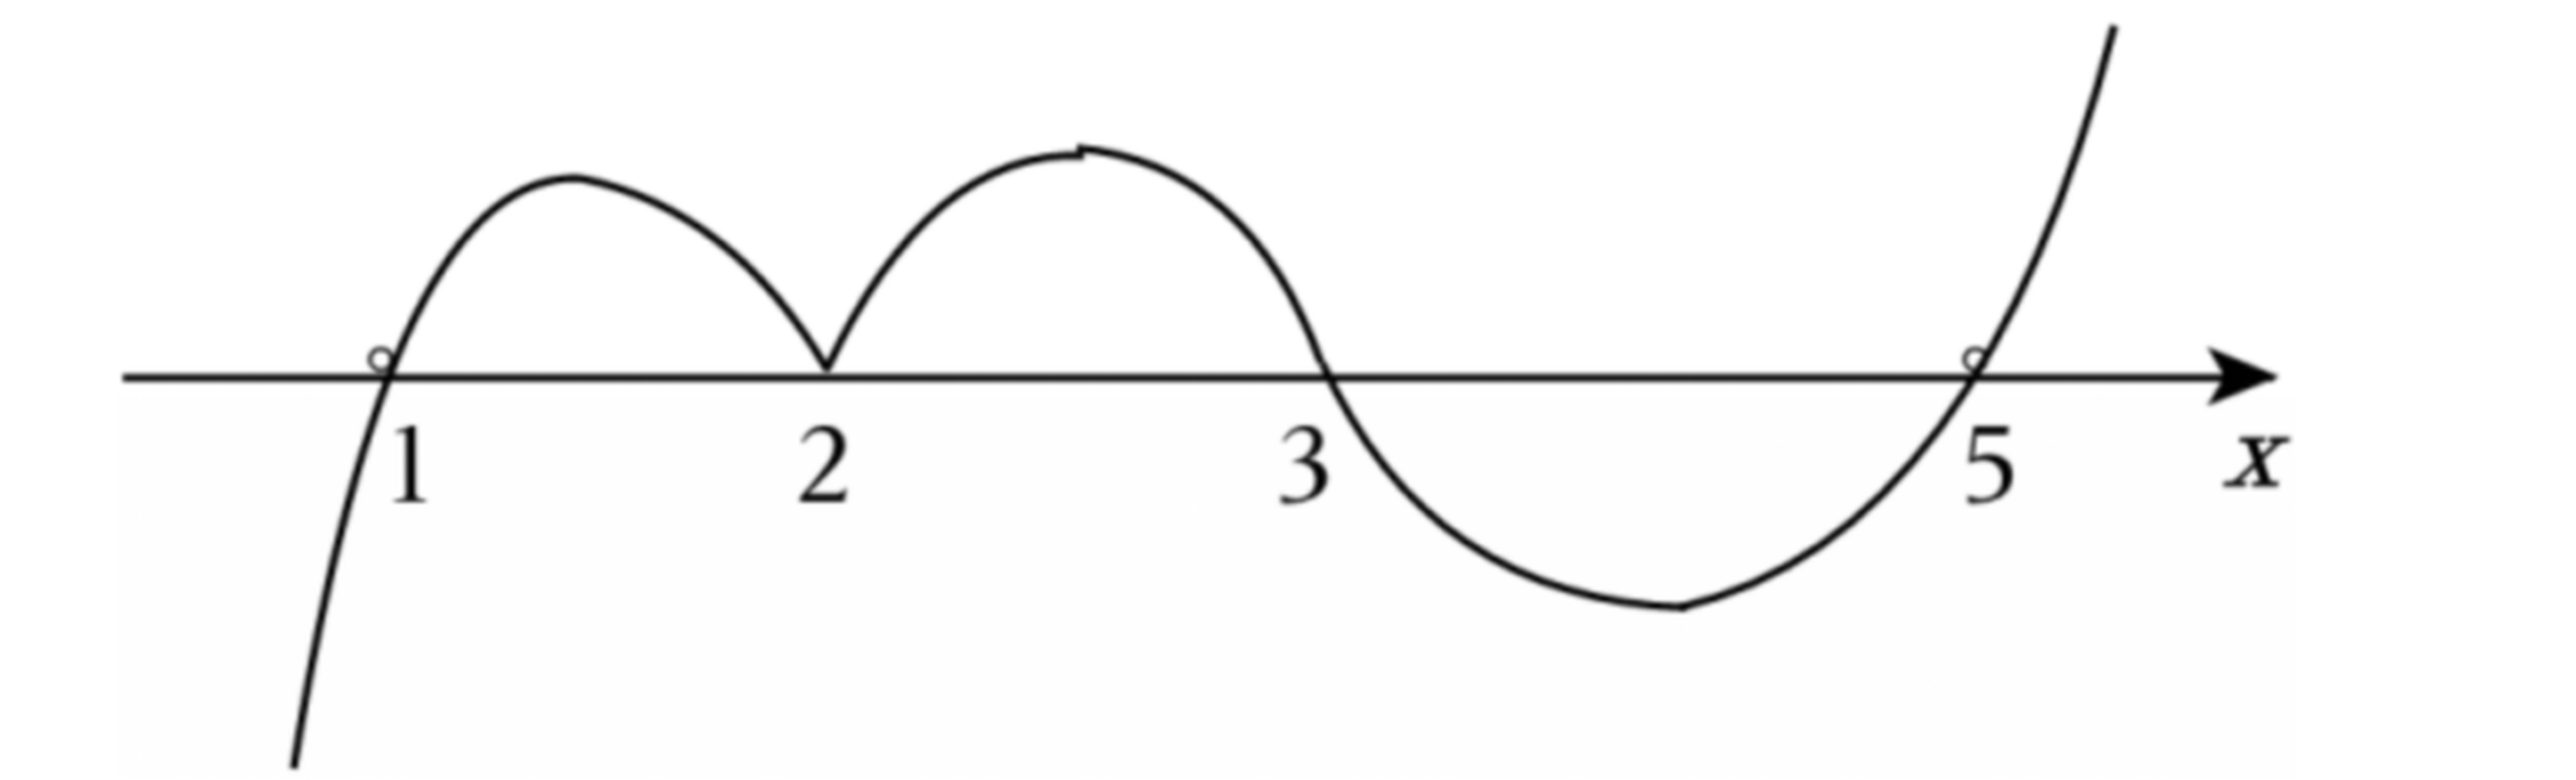
\includegraphics[width=0.62\textwidth]{figures/gao145_q16_a3.png}
\end{center}
\step{得不等式的解集为 $\{x\mid x<1\text{ 或 }x=2\text{ 或 }3\leqslant x<5\}$，}
\step{对应的正整数解为 $2$，$3$，$4$，满足题意，故排除 $B$、$D$；}
\step{当 $a=7$ 时，}
\begin{center}
% a=7 数轴标根图取 06 页，去粉色水印、去色、4× LANCZOS 放大；仅答案版出
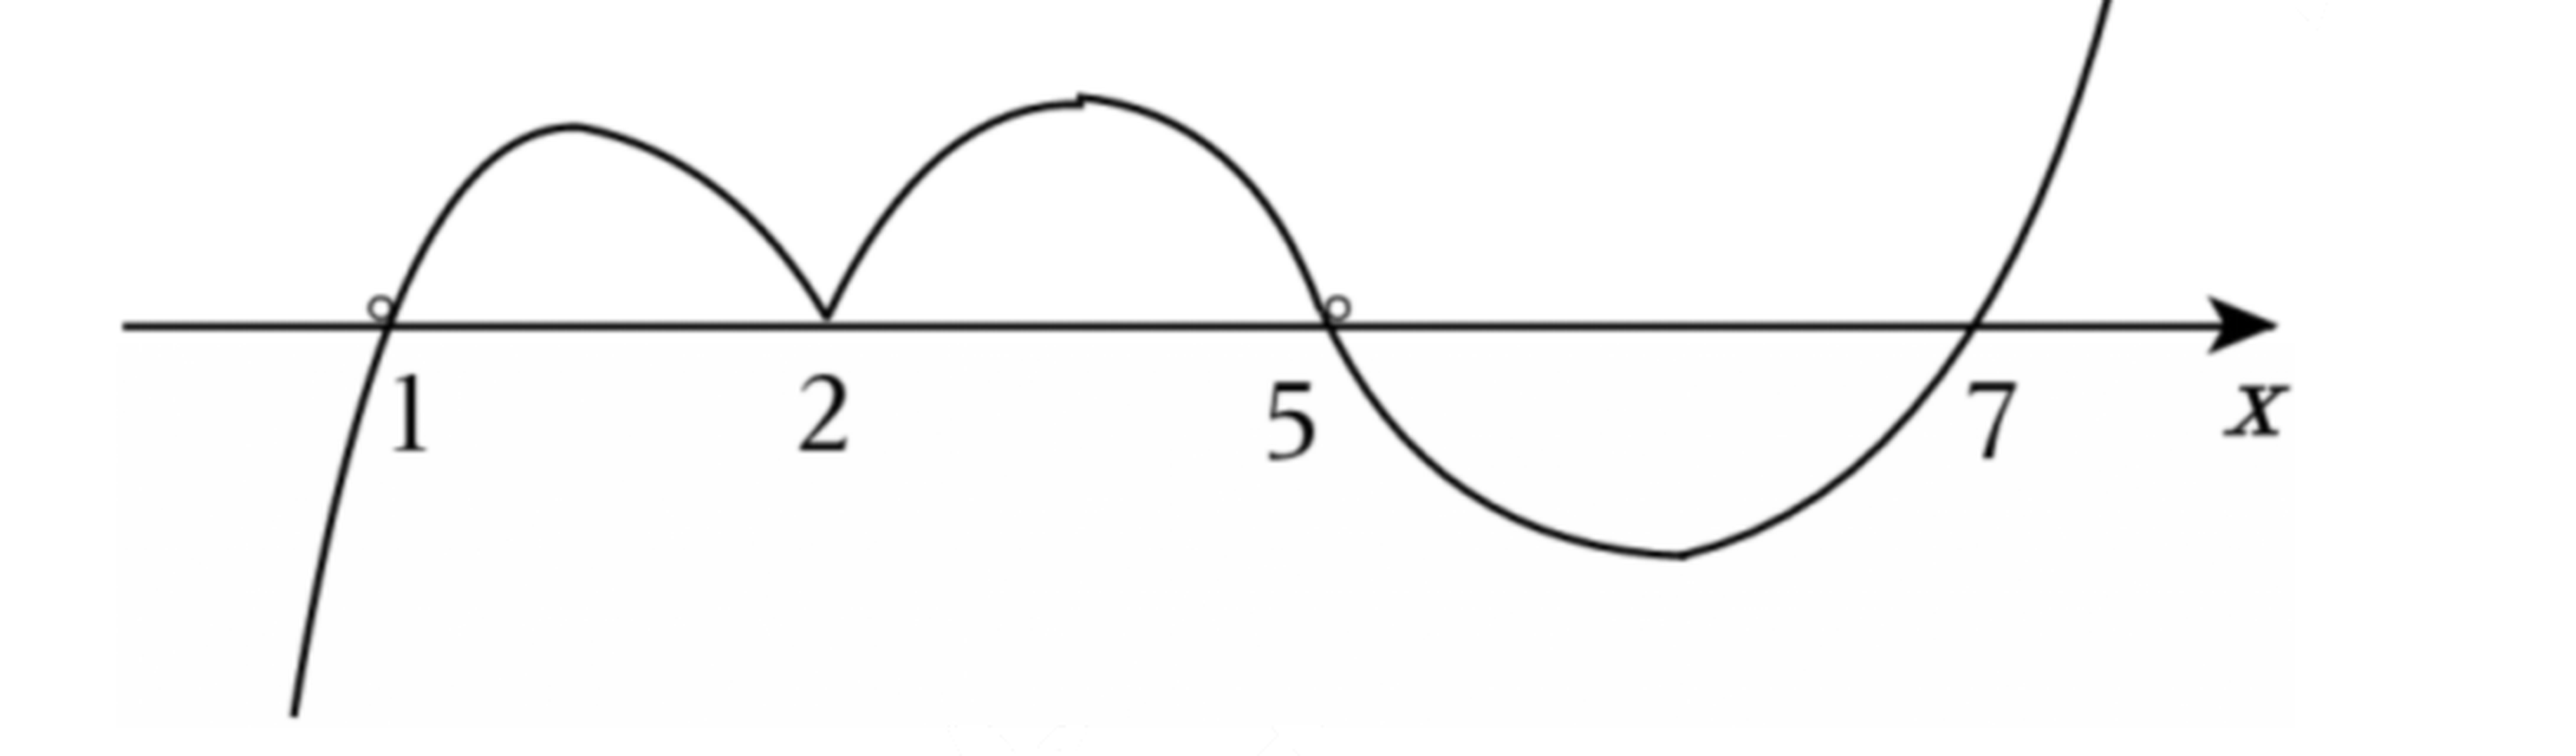
\includegraphics[width=0.62\textwidth]{figures/gao145_q16_a7.png}
\end{center}
\step{得不等式的解集为 $\{x\mid x<1\text{ 或 }x=2\text{ 或 }5<x\leqslant7\}$，}
\step{对应的正整数解为 $2$，$6$，$7$，满足题意，故 $A$ 正确，$C$ 错误.}
\step{故选 $A$.}
\solend
\fi

\end{enumerate}

\bigsec{三、解答题}

\begin{enumerate}
\setcounter{enumi}{16}

% 第 17 题：题干在 06 页、解析续至 07 页，按印刷行断，共 7 行；
% "lg(10÷5)" 的除号照录 \div
\item (1) 已知 $a+a^{-1}=6$，求 $a^2+a^{-2}$ 及 $a^{\frac12}-a^{-\frac12}$ 的值；

(2) 已知 $\lg5=a$，$\lg6=b$，用 $a$、$b$ 分别表示 $\lg2$、$\lg3$、$\lg300$ 和 $\log_{12}15$.

\ifanswer
\solbegin
\step{(1) 因为 $a+a^{-1}=6$，}
\step{所以 $a^2+a^{-2}=(a+a^{-1})^2-2\cdot a\cdot a^{-1}=6^2-2=34$，}
\step{因为 $\left(a^{\frac12}-a^{-\frac12}\right)^2=a-2+a^{-1}=6-2=4$，所以 $a^{\frac12}-a^{-\frac12}=\pm2$；}
\step{(2) $\lg2=\lg(10\div5)=\lg10-\lg5=1-a$，}
\step{$\lg3=\lg(6\div2)=\lg6-\lg2=b-(1-a)=a+b-1$，}
\step{$\lg300=\lg(3\times10^2)=\lg3+\lg10^2=a+b-1+2=a+b+1$，}
\step{所以 $\log_{12}15=\dfrac{\lg15}{\lg12}=\dfrac{\lg3+\lg5}{\lg3+\lg2^2}=\dfrac{a+b-1+a}{a+b-1+2(1-a)}=\dfrac{2a+b-1}{b-a+1}$.}
\solend
\fi

% 第 18 题：题干在 07 页、解析续至 08 页（2 问、分类讨论很长），按印刷行断共 25 行；
% 本卷 Q18 用"图像"（Q13/Q14 用"图象"），逐处照录不统一
\item 已知 $f(x)=(m^2-3m+1)x^{m^2-4m-1}$，$y=f(x)$ 为幂函数且在 $(0,+\infty)$ 上是严格减函数.

(1) 求实数 $m$ 的值以及相应的函数表达式；

(2) 若 $y=f(x)$ 的图像关于 $y$ 轴对称，解关于 $x$ 的不等式 $(x+2)^{1-m}<(3x-1)^{1-m}$.

\ifanswer
\solbegin
\step{(1) 由幂函数的定义得 $m^2-3m+1=1$，}
\step{整理得 $m^2-3m=0$，解得 $m=0$ 或 $m=3$，}
\step{由于 $y=f(x)$ 在 $(0,+\infty)$ 上为严格减函数，}
\step{因此幂函数的指数需满足 $m^2-4m-1<0$，}
\step{当 $m=3$ 时，指数为 $3^2-4\times3-1=-4<0$，满足严格递减条件，}
\step{此时函数表达式为 $f(x)=x^{-4}$，}
\step{当 $m=0$ 时，指数为 $0^2-4\times0-1=-1<0$，满足严格递减条件，}
\step{此时函数表达式为 $f(x)=x^{-1}$，}
\step{所以满足条件的实数 $m$ 为 $0$ 或 $3$，}
\step{对应的函数表达式分别为 $f(x)=x^{-1}$、$f(x)=x^{-4}$；}
\step{(2) 函数图像关于 $y$ 轴对称即函数为偶函数，}
\step{对于 $f(x)=x^{-1}=\dfrac1x$，定义域为 $(-\infty,0)\cup(0,+\infty)$，}
\step{满足 $f(-x)=-f(x)$，为奇函数，图像关于原点对称，}
\step{不满足关于 $y$ 轴对称的条件；}
\step{对于 $f(x)=x^{-4}=\dfrac{1}{x^4}$，定义域为 $(-\infty,0)\cup(0,+\infty)$，}
\step{满足 $f(-x)=f(x)$，为偶函数，图像关于 $y$ 轴对称，}
\step{因此符合条件的 $m$ 值为 $3$，}
\step{将 $m=3$ 代入关于 $x$ 的不等式 $(x+2)^{1-m}<(3x-1)^{1-m}$，}
\step{得 $(x+2)^{1-3}<(3x-1)^{1-3}$，即 $(x+2)^{-2}<(3x-1)^{-2}$，}
\step{因为负指数幂的底数不能为 $0$，所以 $x+2\ne0$ 且 $3x-1\ne0$，}
\step{即 $x\ne-2$ 且 $x\ne\dfrac13$，}
\step{不等式可变形为 $\dfrac{1}{(x+2)^2}<\dfrac{1}{(3x-1)^2}$，}
\step{整理得 $(3x-1)^2<(x+2)^2$，即 $8x^2-10x-3<0$，}
\step{解得 $-\dfrac14<x<\dfrac32$，又 $x\ne-2$ 且 $x\ne\dfrac13$，}
\step{所以不等式的解集为 $\left(-\dfrac14,\dfrac13\right)\cup\left(\dfrac13,\dfrac32\right)$.}
\solend
\fi

% 第 19 题：题干在 08 页、解析续至 09 页，按印刷行断，共 14 行；
% 判别式 cases 块内"△=4a²−16a<0"原卷印扁等边三角 \triangle
%（放大 09 页 zz09_delta.png 与 Q12 高 \Delta 并排确认），逐处照录不统一
\item 已知 $f(x)=ax^2+2ax+4$，$a\in\R$.

(1) 若关于 $x$ 的不等式 $f(x)>0$ 在实数集 $\R$ 上恒成立，求实数 $a$ 的取值范围；

(2) 当 $a<0$ 时，解关于 $x$ 的不等式 $f(x)>(a+1)x+5$.

\ifanswer
\solbegin
\step{(1) 由题意得，关于 $x$ 的不等式 $f(x)>0$ 在实数集 $\R$ 上恒成立，}
\step{即 $ax^2+2ax+4>0$ 在实数集 $\R$ 上恒成立，}
\step{当 $a=0$ 时，不等式为 $4>0$ 恒成立，符合题意；}
\step{当 $a\ne0$ 时，则 $\begin{cases}a>0\\\triangle=4a^2-16a<0\end{cases}$，解得 $0<a<4$.}% 判别式原卷印扁等边三角 $\triangle$，照录
\step{综上所述，实数 $a$ 的取值范围为 $[0,4)$.}
\step{(2) $f(x)=ax^2+2ax+4$，}
\step{当 $a<0$ 时，不等式 $f(x)>(a+1)x+5$ 即为 $ax^2+(a-1)x-1>0$，}
\step{即 $(ax-1)(x+1)>0$，即 $\left(x-\dfrac1a\right)(x+1)<0$，}
\step{当 $a<-1$，即 $\dfrac1a>-1$ 时，解得 $-1<x<\dfrac1a$；}
\step{当 $a=-1$，即 $\dfrac1a=-1$ 时，解得 $x\in\varnothing$；}
\step{当 $-1<a<0$，即 $\dfrac1a<-1$ 时，解得 $\dfrac1a<x<-1$.}
\step{综上所述，当 $a<-1$ 时，不等式的解集为 $\left\{x\mid -1<x<\dfrac1a\right\}$；}
\step{当 $a=-1$ 时，不等式的解集为 $\varnothing$；}
\step{当 $-1<a<0$ 时，不等式的解集为 $\left\{x\mid \dfrac1a<x<-1\right\}$.}
\solend
\fi

% 第 20 题：菜园靠墙图为题目配图（三版都出），题干写"如图"；
% 题干在 09 页（含图）、解析续至 10 页，按印刷行断，共 13 行
\needvspace{8cm}
\item 如图，某人计划用篱笆围成一个一边靠墙（墙足够长）的矩形菜园. 设菜园的长为 $x$ 米，宽为 $y$ 米.

\begin{center}
% 矩形菜园靠墙图取 09 页右下，去粉色水印、去色、4× LANCZOS 放大
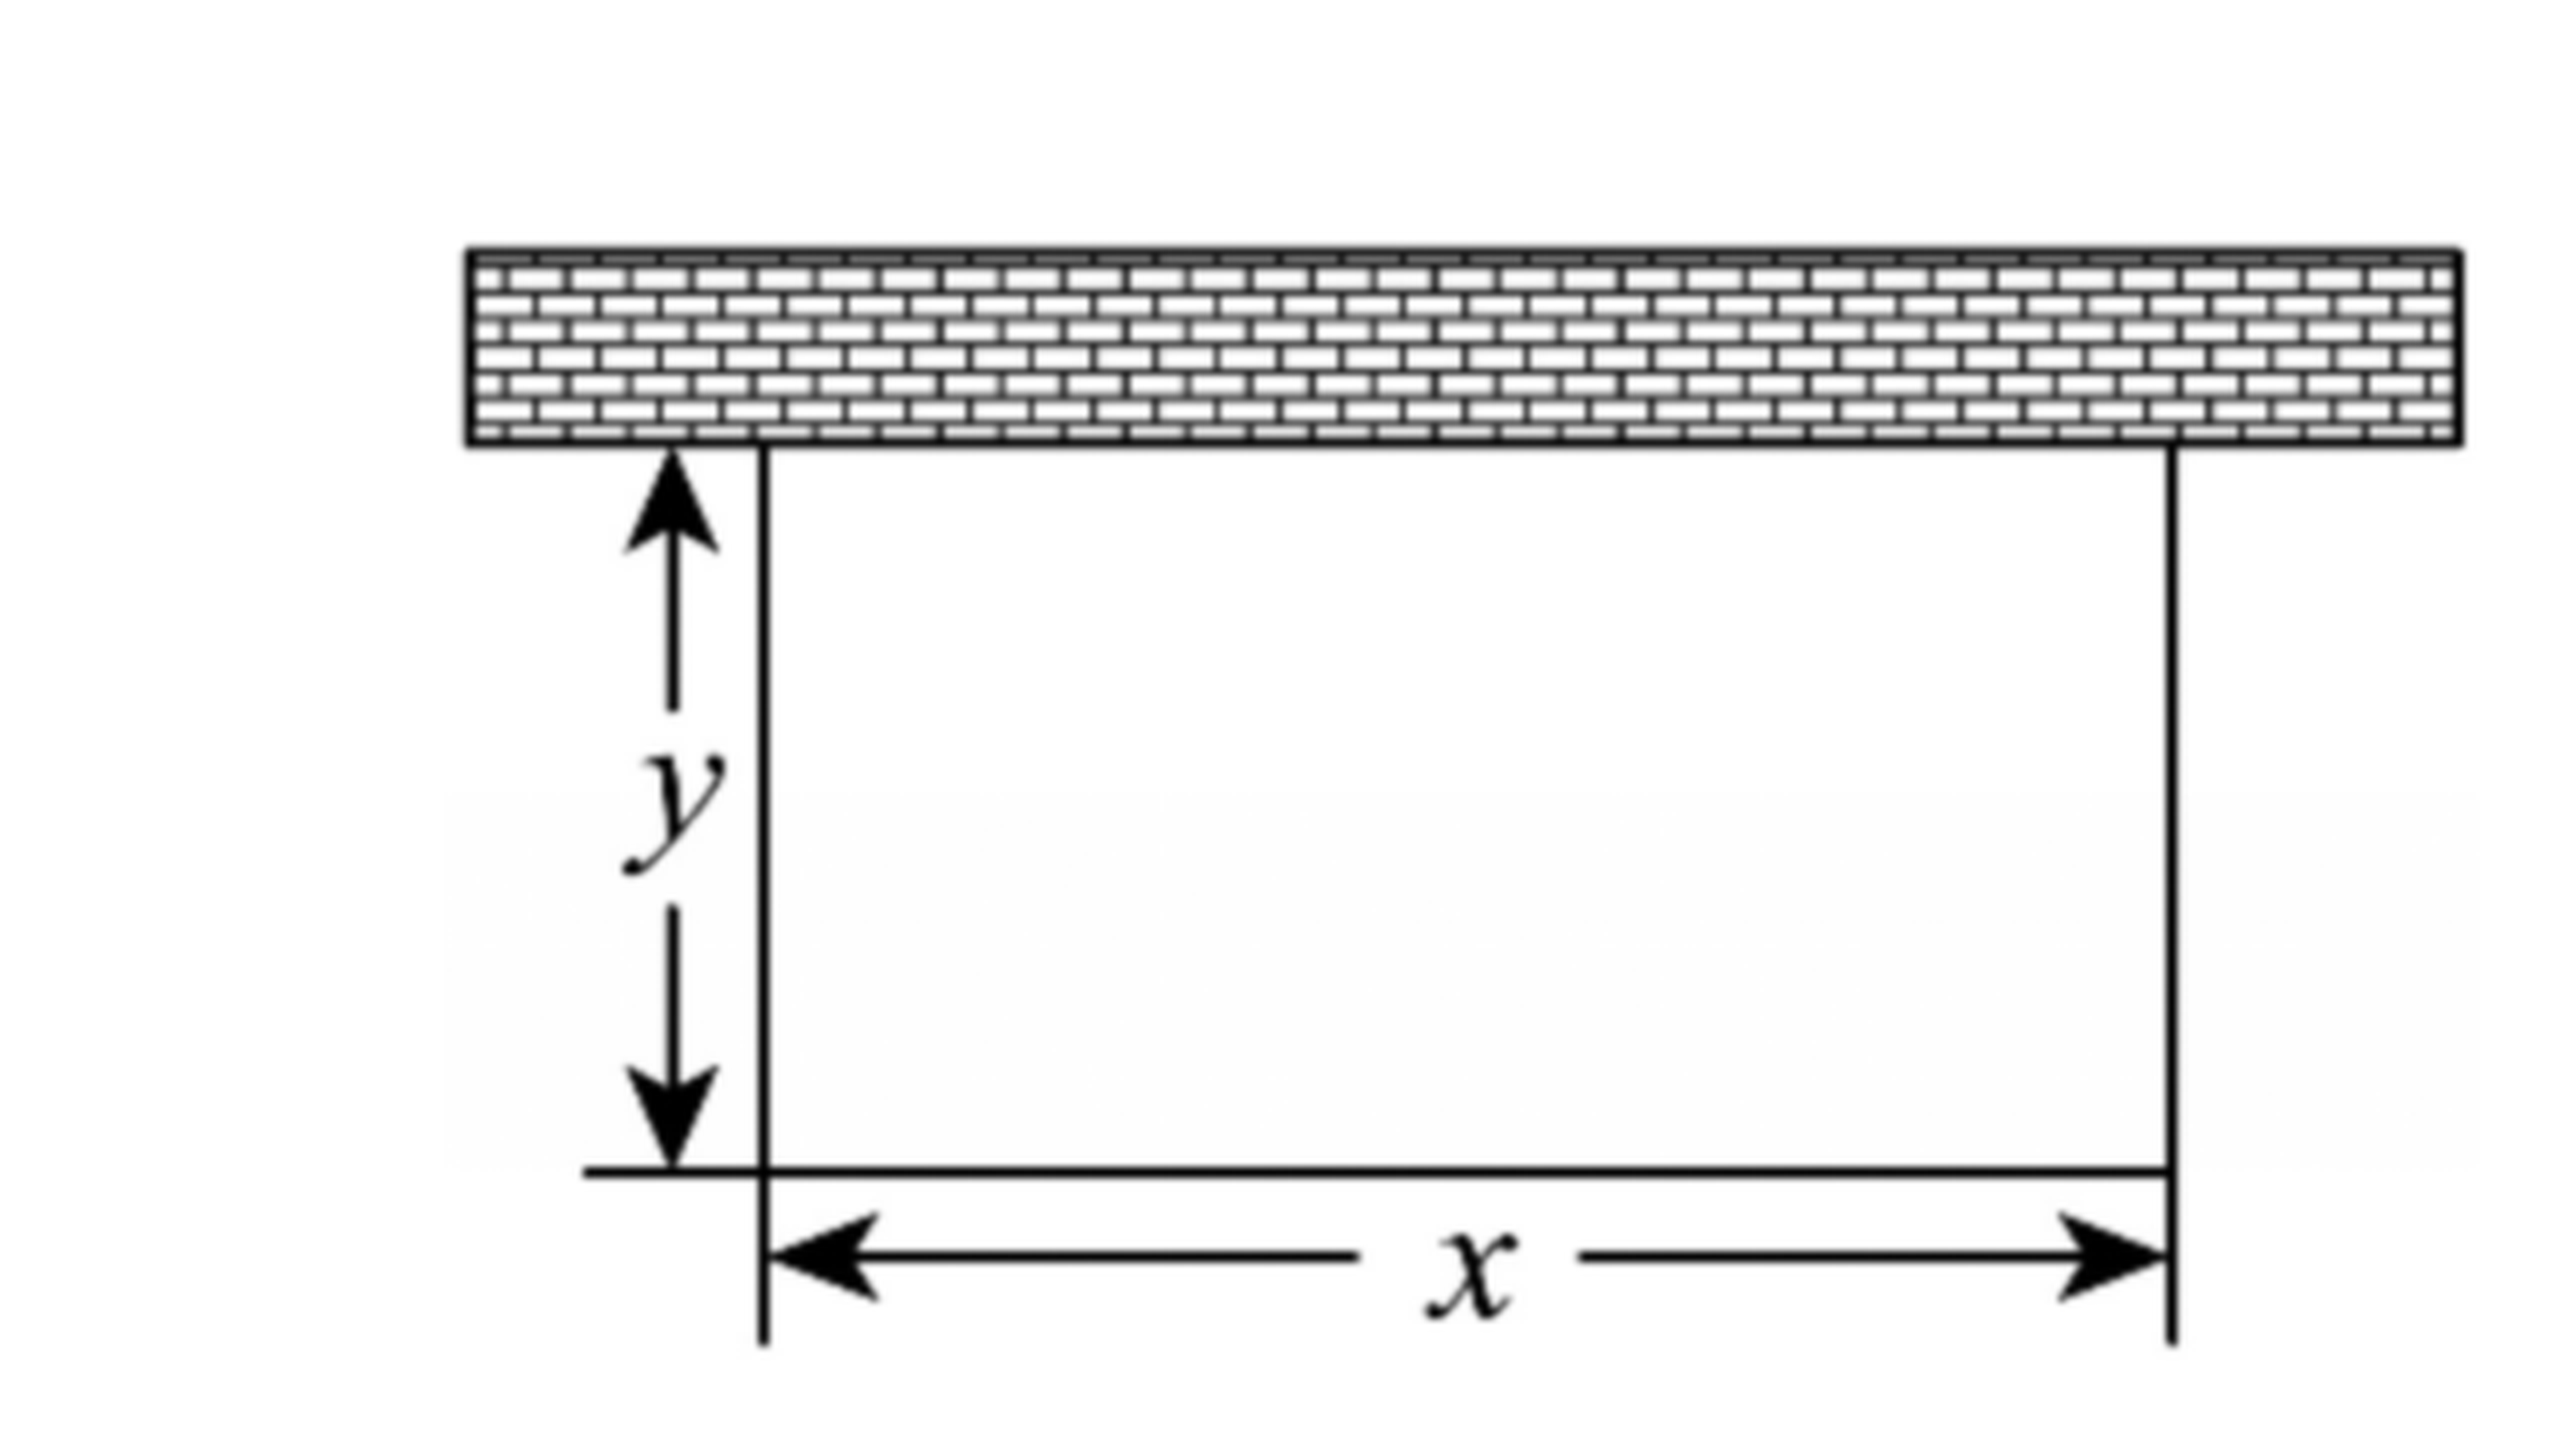
\includegraphics[width=0.55\textwidth]{figures/gao145_q20.png}
\end{center}

(1) 若菜园面积为 72 平方米，则 $x$、$y$ 为何值时，所用篱笆总长最小？

(2) 若 $x$、$y$ 满足 $x+y-xy+63=0$，则菜园面积最小为多少平方米？

\ifanswer
\solbegin
\step{(1) 由题意得，菜园的面积 $S=xy=72$，且 $x>0$，$y>0$，}
\step{所用篱笆总长 $L=x+2y$，}
\step{由基本不等式得 $x+2y\geqslant2\sqrt{x\cdot2y}=2\sqrt{2xy}=2\sqrt{2\times72}=24$，}
\step{当且仅当 $x=2y$ 时取等号，}
\step{联立 $\begin{cases}xy=72\\x=2y\end{cases}$，解得 $\begin{cases}x=12\\y=6\end{cases}$，}
\step{所以当 $x=12$，$y=6$ 时，所用篱笆总长最小；}
\step{(2) 由题意得 $x>0$，$y>0$，且满足 $x+y-xy+63=0$，即 $x+y=xy-63$，}
\step{由基本不等式得 $x+y\geqslant2\sqrt{xy}$，当且仅当 $x=y$ 时取等号，}
\step{所以 $xy-63\geqslant2\sqrt{xy}$. 令 $t=\sqrt{xy}(t>0)$，则 $xy=t^2$，}
\step{上述不等式可化为 $t^2-2t-63\geqslant0$，即 $(t-9)(t+7)\geqslant0$，}
\step{因为 $t>0$，所以 $t+7>0$，故 $t-9\geqslant0$，解得 $t\geqslant9$，所以 $\sqrt{xy}\geqslant9$，}
\step{即 $xy\geqslant81$，当且仅当 $x=y=9$ 时取等号，此时满足 $9+9-81+63=0$，}
\step{所以菜园面积最小为 81 平方米.}
\solend
\fi

% 第 21 题：题干在 10 页、解析续至 11 页（3 问、分类讨论很长），按印刷行断共 22 行；
% 末行"故第 2026 个元素是 2700 之后第一个属于 A 的数，即 2701." 为全卷收尾，
% 无 Q22/Q23、无附加题节；数集 Z/N* 按全稿惯例改 \Z/\N^*
\item 已知集合 $A=\{x\mid x=m^2-n^2$，$m$、$n\in\Z\}$.

(1) 求证：任何奇数 $2k+1(k\in\Z)$ 都是集合 $A$ 中的元素；

(2) 判断偶数 $4k-2(k\in\Z)$ 是否为集合 $A$ 的元素？请说明理由；

(3) 若将集合 $A$ 中的正整数由小到大排列，求出集合 $A$ 中第 2026 个正整数.

\ifanswer
\solbegin
\step{(1) 因为 $x=(k+1)^2-k^2=2k+1(k\in\Z)$，}
\step{所以任何奇数 $2k+1(k\in\Z)$ 都属于集合 $A$；}
\step{(2) 偶数 $4k-2(k\in\Z)$ 不是集合 $A$ 的元素，理由如下：}
\step{由题意得 $x=m^2-n^2=(m-n)(m+n)$，}
\step{当 $m$、$n$ 均为奇数时，设 $m=2k_1+1$，$n=2k_2+1(k_1$、$k_2\in\Z)$，}
\step{则 $m^2-n^2=(2k_1+1)^2-(2k_2+1)^2=(2k_1-2k_2)(2k_1+2k_2+2)$}
\step{$=4(k_1-k_2)(k_1+k_2+1)$，}
\step{因为 $k_1$、$k_2\in\Z$，所以 $k_1-k_2\in\Z$，$k_1+k_2+1\in\Z$，}
\step{从而 $m^2-n^2$ 为 $4$ 的倍数；}
\step{当 $m$、$n$ 均为偶数时，设 $m=2k_1$，$n=2k_2(k_1$、$k_2\in\Z)$，}
\step{$m^2-n^2=4k_1^2-4k_2^2=4(k_1^2-k_2^2)$ 为 $4$ 的倍数；}
\step{当 $m$、$n$ 为一个偶数一个奇数时，不妨设 $m$ 为偶数，$n$ 为奇数，}
\step{设 $m=2k_1$，$n=2k_2+1(k_1$、$k_2\in\Z)$，}
\step{则 $m^2-n^2=4k_1^2-(2k_2+1)^2=4(k_1^2-k_2^2-k_2)-1$ 为奇数.}
\step{无论哪种情况均不满足 $4k-2(k\in\Z)$，}
\step{故偶数 $4k-2(k\in\Z)$ 不是集合 $A$ 的元素；}
\step{(3) 由前两问得，$4$ 的倍数和奇数属于集合 $A$ 中的元素，}
\step{令集合 $A$ 中的正整数元素为 $4k-3$、$4k-1$、$4k(k\in\N^*)$，}
\step{对任意的 $k\in\N^*$，连续的 $4$ 个整数 $4k-3$、$4k-2$、$4k-1$、$4k$ 中}
\step{有三个数 $4k-3$、$4k-1$、$4k$ 都在集合 $A$ 中，}
\step{因为 $2026=3\times675+1$，所以集合 $A$ 中第 $2025$ 个元素为 $4\times675=2700$，}
\step{故第 2026 个元素是 2700 之后第一个属于 $A$ 的数，即 2701.}
\solend
\fi

\end{enumerate}

\end{document}
"
% 紧凑版：xelatex "\def\iscompact{1}% 高一145_市二中学_期中.tex
%   —— 高一上数学"2026-2027 年市二中学高一上期中"（试卷版/答案版/紧凑版）
% 试卷版：xelatex 高一145_市二中学_期中.tex
% 答案版：xelatex "\def\isanswer{1}\input{高一145_市二中学_期中.tex}"
% 紧凑版：xelatex "\def\iscompact{1}\input{高一145_市二中学_期中.tex}"
%
% ① 原始材料：微信公众号"魔都数学加油站"文章，连载"27学年高一145"，原文标题
% "27学年高一145——2026-2027年上海市市二中学高一上期中"；
% 原文链接：https://mp.weixin.qq.com/s/6V-i9KE0GWodC-wmd5z8nQ 。
% 正文为 11 张 PNG 页（01/02/03/08/10/11 为 4762×6735，04/05/06/07/09 为 2560×3620，
% 同一篇各页分辨率不同，逐页按各自分辨率裁图核对，别按预览比例换算裁框）。
% 题目下印【答案】或【解析】，为混合体例讲评版：Q3 只印【答案】、无【解析】，其余
% 18 题印【解析】。题目、解析均据原图转录；卷面粉红色水印"魔都数学加油站"及
% 公众号页脚未录入。
% 全卷插图情况（逐页通读 11 页确认，题干写"如图"处均配有图）：
%   · Q14 韦恩图（05 页右侧，全集 U 矩形＋两圆 M/N＋白色交集、灰色阴影＋U/M/N 标注）：
%     题目配图（选择题选项旁），三版都出，裁自 05 页去水印去色 4× 放大存
%     figures/gao145_q14.png；
%   · Q16 两幅数轴标根波浪曲线（06 页，a=3 与 a=7 各一幅，标根法画
%     (x-1)(x-2)^2(x-5)(x-a)≤0 的符号曲线）：【解析】内的配图，仅答案版出，
%     裁 figures/gao145_q16_a3.png / figures/gao145_q16_a7.png（或合并一张），
%     放在答案版条件块内 \solbegin 的 \step 之间（照 高一73 第 16 题成例）；
%   · Q20 矩形菜园靠墙图（09 页右下，灰色砖墙＋矩形菜园＋x/y 标注＋箭头）：
%     题目配图，三版都出，裁自 09 页去水印去色 4× 放大存 figures/gao145_q20.png；
%   其余各页逐页确认无其它题目配图、无表格、亦无"题干写如图而源码漏图"一处。
%
% 卷首标题：原卷印作"2026-2027 年市二中学高一上期中"，年份区间按全稿惯例排 en dash；
% 原卷卷面未印副标题，本稿按同期中卷（高一140／141／143／144）知识模块口径补出
% "集合与常用逻辑用语、不等式、函数"。
%
% 题号体例：本卷共 19 题——一、填空题 3—12（10 题）、二、选择题 13—16（4 题）、
% 三、解答题 17—21（5 题）。三节分别 \setcounter{enumi}{2}／{12}／{16}。
% 原卷从第 3 题起、无第 1、2 题，本稿保留原题号；全卷无附加题节。
%
% ② 与原卷的排版差异：
%   ① 原文从第 3 题起，本稿保留原题号；共 19 题三节；
%   ② 混合体例：原卷 Q3 只印【答案】、无【解析】（"第一步应假设___。
%      【答案】x≤2 或 y≤2"），按 高一140 第 5 题成例提 \ans{}、不补造解析；
%      其余 18 题印【解析】，用 \solbegin…\solend，选择题答案在解析末句"故选 X"
%      （Q13 选 B、Q14 选 D、Q15 选 D、Q16 选 A，逐个放大原图核实）、
%      题干括号 \mbox{（\quad）} 留空、不另提 \ans{}；填空／解答答案落在解析里；
%      答案版【答案】/【解析】标记数 = 19（1 个 \ans ＋ 18 个 \solbegin）= 全卷题数；
%   ③ 原卷卷面未印副标题，本稿按知识模块口径补出；
%   ④ 原卷填空横线按全稿惯例排 \blankline[4.4em]；选择题括号排 \mbox{（\quad）}、
%      选项段前按惯例加 \keepwithprev；解答题不留作答区、不加 \anspace
%      （原卷为讲评版，与 129／131／132／133／136／140／141／143／144 同）；
%   ⑤ 数集：Q9"a、b∈R"、Q12"a∈R"、Q21"m、n∈Z""k∈Z""k∈N*"等原卷印
%      斜体或黑板粗体 R/Z/N，按全稿惯例统一改 \R／\Z／\N^*；绝对值排 \lvert…\rvert，
%      集合描述竖线排 \mid；不等号按全稿惯例排 \leqslant／\geqslant；
%      补集照原卷上划线排 \overline{M}／\overline{N}（Q14 选项 B/C/D 逐处核）；
%      空集记号 \varnothing；\subset（单线⊂）与 \subseteq（带下划线⊆）逐处照录不统一；
%   ⑥ 子题标号 (1)(2)(3) 原卷印半角括号照录；圈数字进数学式用 \text{①}（否则 FONTCHK 挂）；
%      \left…\right 不得拆到不同 $…$ 组；cases 块整体算一个印刷行；
%   ⑦ 题干／解析中的中文弯引号按原卷照录（Q3"若 x+y>4，则 x>2 且 y>2"、
%      Q11"a₁/a₂=b₁/b₂""M=N"、选填"充分非必要""必要非充分""充要""既非充分也非必要"
%      等，含引号内空格），注释内一律 ASCII 引号；数学式内 CJK 用 \text{}；
%   ⑧ 半角逗号在数学组之间是全稿惯例、非笔误（如 Q5"x₁+x₂=6，x₁x₂=√3"、
%      Q7"a>1，b>1"、指数／对数式内逗号），逐处照录别改全角；行末西文句点照录为
%      ASCII `.`；行中全角逗号／顿号照录；
%   ⑨ "图像／图象"逐处照录不统一（Q18"图像关于 y 轴对称"等，核全卷）；
%   ⑩ 判别式 Δ/△ 混用是照录项：Q12 解析"Δ=a²−4a²(2a−3)>0"、
%      Q19 解析"Δ=4a²−16a<0"等，放大原图判断是高 \Delta（等腰偏高、高>宽）
%      还是扁 \triangle，逐处照录不得统一（参照 高一142／144 头注④口径）；
%   ⑪ 一条 \step = 原卷解析的一个印刷行，cases 块整体算一个印刷行；别把原卷折行
%      并起来、别把一行拆多条。Q6 分段讨论、Q12 三个 cases 条件组、Q16 数轴标根、
%      Q18／Q19 分类讨论、Q21 三问均按印刷行逐条断，不丢行；
%   ⑫ Q14 韦恩图为"题干＋选项＋图"整块，加 \needvspace 守卫推走（守卫放 \item 之前，
%      见 高一140 Q14、高一144 Q17 成例与切页审计 B 类坑）；Q20 菜园图同理；
%      三版切页审计均"合计异常：无"；
%   ⑬ 跨页续印按题合并：Q3/4/5/6 在 01 页（Q6 解析续 02 页顶）；Q7/8/9/10 在 02 页
%      （Q10 解析续 03 页）；Q11/12 在 03 页（Q12 解析续 04 页，很长）；
%      Q13 在 04 页末、解析在 05 页顶；Q14/15/16 在 05 页（Q16 解析续 06 页含两幅数轴图）；
%      Q17 在 06 页、解析续 07 页；Q18 在 07 页、解析续 08 页；Q19 在 08 页、解析续 09 页；
%      Q20 在 09 页（含菜园图）、解析续 10 页；Q21 在 10 页、解析续 11 页
%      （末页收尾"故第 2026 个元素是 2700 之后第一个属于 A 的数，即 2701."、
%      无 Q22/Q23、无附加题节）。本稿按题连排，不丢行、不并折行；
%   ⑭ 原卷解析内若有红色"法一／法二"之类小标题，按全稿惯例排 \stepm{标签}{…}
%      （黑体着色、不引入红色、不改 common.sty），头注注明；水印"魔都数学加油站"
%      红色不录入。
%
% ③ 行数复核：一条 \step／\stepm = 原卷解析的一个印刷行，cases 块作一个印刷行计。
%   逐题数（主会话逐页核对定稿）：Q3：0（只印【答案】、提 \ans{}，不计入 \step 账）；
%   Q4：3；Q5：2；Q6：10；Q7：3；Q8：3；Q9：2；Q10：7；Q11：4；Q12：12；
%   Q13：2；Q14：2；Q15：4；Q16：9；Q17：7；Q18：25；Q19：14；Q20：13；Q21：22。
%   合计 144 条 \step（本卷无 \stepm：解析内无红色"法一／法二"类小标题），
%   与原卷逐题印刷行相等。全卷 18 题设 \solbegin…\solend ＋ Q3 一处 \ans{}，
%   答案版【答案】/【解析】标记数 = 19 = 全卷题数。
%
% ④ 判别式／子集符号结论（逐处放大原图照录、不得统一，主会话像素级复核）：
%   判别式全卷 2 处、两形混用逐处照录不统一（参照 高一142／144 头注④口径）：
%     · Q12 解析 cases 块"Δ=a²−4a²(2a−3)>0" 原卷印等腰偏高粗三角（高>宽），
%       照录 \Delta（放大 04 页 /tmp/gao145s2/main_q12_delta.png 确认）；
%     · Q19 解析 cases 块"△=4a²−16a<0" 原卷印扁等边空心三角（宽≈高、细线），
%       照录 \triangle（放大 09 页 /tmp/gao145s2/main_q19_delta.png 确认）。
%   子集／补集：Q14 选项 A `M\cup N`、B `M\cap\overline{N}`（上划线只在 N 上）、
%   C `\overline{M\cup N}`（罩整个 M∪N）、D `\overline{M\cap N}`（罩整个 M∩N，
%   非 \overline{M}\cap N；放大 05 页 /tmp/gao145s2/main_q14_opts.png 确认），
%   阴影为灰色区域＝全集减白色交集，答案 D，照录 \overline{M\cap N}；
%   全集卷无 \subset／\subseteq 混用（本卷集合题用 \cup／\cap／\overline{}）；
%   空集 \varnothing（Q19 解析 x∈\varnothing）；数集 \R／\Z／\N^* 归一见 ② ⑤。
%
% ⑤ 存疑照录（放大原图确认，照录未改、正文对应处另有 % 注）：
%   1. Q3 题干"若 x+y>4，则 x>2 且 y>2" 后"时"前留一空格、弯引号内空格照录；
%      该卷混合体例（Q3 只印【答案】、提 \ans{}）见 ② ②。
%   2. Q4／Q5 解析中的"1，3，5 和 6"、"x₁+x₂=6,x₁x₂=√3" 等半角／全角逗号
%      逐处照原卷（放大 01 页确认），数学式内半角逗号为全稿惯例、非笔误。
%   3. Q14 选项 D 上划线罩住整个 M∩N（而非仅罩 M），照录 \overline{M\cap N}。
%   4. Q12 判别式高 \Delta 与 Q19 判别式扁 \triangle 两形混用，逐处照录不统一（见 ④）。
%   全卷除此 4 类外未发现其它笔误／自相矛盾处。
%
% ⑥ 跨页续印按题合并说明：见 ② ⑬。
%
\documentclass[a4paper,11pt]{article}
\usepackage{common}

\begin{document}

\examtitlest[3]{2026--2027 年市二中学高一上期中}{集合与常用逻辑用语、不等式、函数}

\bigsec{一、填空题}

\begin{enumerate}
\setcounter{enumi}{2}

% 第 3 题：原卷只印【答案】、无【解析】（放大 01 页确认），按 高一140 第 5 题成例
% 提 \ans{}、不补造解析；题干中文弯引号与"时"前空格照录
\item 用反证法证明命题：“若 $x+y>4$，则 $x>2$ 且 $y>2$” 时，第一步应假设\blankline[4.4em].

\ifanswer
\ans{$x\leqslant2$ 或 $y\leqslant2$}
\fi

% === Q4 ===
\item 设集合 $M$ 满足 $\{1,3,5,6\}\cup M=\{1,2,3,4,5,6\}$，则满足条件的所有 $M$ 的个数为\blankline[4.4em].

\ifanswer
\solbegin
\step{集合 $M$ 满足 $\{1,3,5,6\}\cup M=\{1,2,3,4,5,6\}$，}
\step{则 $M$ 中必含有 $2$ 和 $4$，$1$，$3$，$5$ 和 $6$ 可以选也可不选，}
\step{则满足条件的所有 $M$ 的数目相当于集合 $\{1,3,5,6\}$ 的子集的个数 $2^4=16$.}
\solend
\fi

% === Q5 ===
\item 已知方程 $x^2-6x+\sqrt3=0$ 的两根为 $x_1$ 和 $x_2$，则 $(x_1-x_2)^2=$\blankline[4.4em].

\ifanswer
\solbegin
\step{因为方程 $x^2-6x+\sqrt3=0$ 的两根为 $x_1$ 和 $x_2$，所以 $x_1+x_2=6,x_1x_2=\sqrt3$，}% 数学式内半角逗号为全稿惯例，照录
\step{所以 $(x_1-x_2)^2=(x_1+x_2)^2-4x_1x_2=36-4\sqrt3$.}
\solend
\fi

% 第 6 题：题干在 01 页，解析续至 02 页顶（末 2 行），按印刷行逐条断，共 10 行
\item 不等式 $\lvert x-2026\rvert+\lvert x-2029\rvert>3$ 的解集是\blankline[4.4em].

\ifanswer
\solbegin
\step{当 $x<2026$ 时，$x-2026<0$，$x-2029<0$，}
\step{原不等式可化为 $(2026-x)+(2029-x)>3$，解得 $x<2026$，}
\step{故此时，不等式的解为 $x<2026$；}
\step{当 $2026\leqslant x\leqslant2029$ 时，$x-2026\geqslant0$，$x-2029\leqslant0$，}
\step{原不等式可化为 $(x-2026)+(2029-x)>3$，即 $3>3$，显然不成立，}
\step{故此时，不等式无解；}
\step{当 $x>2029$ 时，$x-2026>0$，$x-2029>0$，}
\step{原不等式可化为 $(x-2026)+(x-2029)>3$，解得 $x>2029$，}
\step{故此时，不等式的解为 $x>2029$.}
\step{综上，原不等式的解集为 $(-\infty,2026)\cup(2029,+\infty)$.}
\solend
\fi

% === Q7 ===
\item 已知 $a>1$，$b>1$，若 $\log_a b+\log_b a=2$，且 $ab=2$，则 $\log_2(a+b)=$\blankline[4.4em].

\ifanswer
\solbegin
\step{由 $\log_a b+\log_b a=2$，$a>1$，$b>1$，得 $\log_a b+\dfrac{1}{\log_a b}=2$，}
\step{即 $(\log_a b)^2-2\log_a b+1=0$，则 $(\log_a b-1)^2=0$，解得 $\log_a b=1$，即 $a=b$，}
\step{又 $ab=2$，所以 $a=b=\sqrt2$，所以 $\log_2(a+b)=\log_2 2\sqrt2=\log_2 2^{\frac32}=\dfrac32$.}
\solend
\fi

% === Q8 ===
\item 已知 $m>0$，$n>0$，且 $m+n=1$，则 $\dfrac1m+\dfrac4n$ 的最小值为\blankline[4.4em].

\ifanswer
\solbegin
\step{由 $m>0$，$n>0$，$m+n=1$，}
\step{则 $\dfrac1m+\dfrac4n=(m+n)\left(\dfrac1m+\dfrac4n\right)=5+\dfrac nm+\dfrac{4m}n\geqslant5+2\sqrt{\dfrac nm\cdot\dfrac{4m}n}=9$，}
\step{当且仅当 $n=2m=\dfrac23$ 时，上式取得等号，故最小值为 $9$.}
\solend
\fi

% === Q9 ===
\item 已知 $a$、$b\in\R$，且 $3a+2b=1$，则 $8^a+4^b$ 最小值为\blankline[4.4em].

\ifanswer
\solbegin
\step{因为 $3a+2b=1$，所以 $8^a+4^b=2^{3a}+2^{2b}\geqslant2\sqrt{2^{3a+2b}}=2\sqrt2$，}
\step{当且仅当 $3a=2b$ 时取等号，故最小值为 $2\sqrt2$.}
\solend
\fi

% 第 10 题：题干在 02 页、解析续至 03 页顶，按印刷行断，共 7 行
\item 已知关于 $x$ 的不等式 $ax^2+bx+c>0$ 的解集为 $\{x\mid 1<x<2\}$，则关于 $x$ 的不等式 $bx^2-ax+c<0$ 的解集为\blankline[4.4em].

\ifanswer
\solbegin
\step{已知关于 $x$ 的不等式 $ax^2+bx+c>0$ 的解集为 $\{x\mid 1<x<2\}$，}
\step{由解集为 $1<x<2$ 且二次函数在两根之间为正，得 $a<0$，两个根为 $1$，$2$，}
\step{所以 $ax^2+bx+c=a(x-1)(x-2)=ax^2-3ax+2a$，}
\step{比较系数得 $b=-3a$，$c=2a$.}
\step{于是 $bx^2-ax+c=-3ax^2-ax+2a=-a(3x-2)(x+1)$，}
\step{$a<0$，故 $bx^2-ax+c<0$ 等价于 $(3x-2)(x+1)<0$，解得 $-1<x<\dfrac23$，}
\step{故 $bx^2-ax+c<0$ 的解集为 $\left\{x\mid -1<x<\dfrac23\right\}$.}
\solend
\fi

% 第 11 题：题干引号内空格照录（放大 03 页确认），四组选填引号亦同；
% 结论"故为必要非充分条件"照录，解析共 4 个印刷行
\item 设 $a_1$、$b_1$、$a_2$、$b_2$ 均为非零实数，不等式 $a_1x+b_1>0$ 和 $a_2x+b_2>0$ 的解集分别为集合 $M$、$N$，那么 “ $\dfrac{a_1}{a_2}=\dfrac{b_1}{b_2}$ ” 是 “ $M=N$ ” 的\blankline[4.4em]条件（选填 “ 充分非必要 ”、“ 必要非充分 ”、“ 充要 ” 和 “ 既非充分也非必要 ”）.

\ifanswer
\solbegin
\step{当 $a_1=b_1=1$，$a_2=b_2=-1$ 时，满足 $\dfrac{a_1}{a_2}=\dfrac{b_1}{b_2}$，}
\step{但是 $M=N$ 不成立，即充分性不成立；}
\step{若 $M=N$ 时，$\dfrac{a_1}{a_2}=\dfrac{b_1}{b_2}$ 一定成立，即必要性成立.}
\step{故为必要非充分条件.}
\solend
\fi

% 第 12 题：题干在 03 页、解析续至 04 页（很长，含 3 个 cases 条件组），
% 按印刷行逐条断共 12 行；cases 块整体算一个印刷行
\item 已知 $f(x)=\dfrac{ax+3}{x-2}$（常数 $a\in\R$）. 函数 $y=f(x)$ 在区间 $[3,+\infty)$ 上是严格减函数，且函数值不恒为负. 若关于 $x$ 的方程 $f(x)=\dfrac{a}{ax-1}$ 有两个不相等的实数根 $x_1$ 和 $x_2$，则 $a$ 的取值范围是\blankline[4.4em].

\ifanswer
\solbegin
\step{$f(x)=\dfrac{ax+3}{x-2}=a+\dfrac{3+2a}{x-2}$，定义域 $(-\infty,2)\cup(2,+\infty)$，}
\step{由于 $y=f(x)$ 在区间 $[3,+\infty)$ 上是严格减函数，且函数值不恒为负，}
\step{所以 $\begin{cases}3+2a>0\\a+\dfrac{3+2a}{3-2}\geqslant0\end{cases}\Rightarrow a\geqslant-1$，}
\step{若关于 $x$ 的方程 $f(x)=\dfrac{a}{ax-1}$ 有两个不相等的实数根 $x_1$ 和 $x_2$，}
\step{则 $\dfrac{ax+3}{x-2}=\dfrac{a}{ax-1}$，即 $(ax+3)(ax-1)=a(x-2)$，$x\ne2$ 且 $ax-1\ne0$，}
\step{当 $a\ne0$ 且 $a\geqslant-1$ 时，$(ax+3)(ax-1)=a(x-2)$，$x\ne2$ 且 $ax-1\ne0$，}
\step{可化为 $\begin{cases}a^2x^2+ax+2a-3=0\\x\ne2,x\ne\dfrac1a\end{cases}$，}
\step{要使方程有两个不相等的实数根 $x_1$ 和 $x_2$，}
\step{则 $\begin{cases}\Delta=a^2-4a^2(2a-3)>0\\a\geqslant-1\text{且}a\ne0\\4a^2+2a+2a-3\ne0\\a^2\cdot\dfrac1{a^2}+a\cdot\dfrac1a+2a-3\ne0\end{cases}\Rightarrow\begin{cases}a<\dfrac{13}{8}\\a\geqslant-1\text{且}a\ne0\\a\ne\dfrac12\text{且}a\ne-\dfrac32\\a\ne\dfrac12\end{cases}$，}% 判别式原卷印等腰偏高三角 $\Delta$，照录（放大 04 页 zz04_delta.png 确认）
\step{得 $-1\leqslant a<\dfrac{13}{8}$ 且 $a\ne0,a\ne\dfrac12$；}
\step{当 $a=0$ 时，方程无解；}
\step{所以 $a$ 的取值范围是 $[-1,0)\cup\left(0,\dfrac12\right)\cup\left(\dfrac12,\dfrac{13}{8}\right)$.}
\solend
\fi

\end{enumerate}

\bigsec{二、选择题}

\begin{enumerate}
\setcounter{enumi}{12}

% 第 13 题：题干在 04 页末、解析在 05 页顶；"图象"照录（本卷 Q13、Q14 用"图象"）
\item 已知幂函数 $f(x)$ 的图象过点 $\left(7,\dfrac{1}{\sqrt7}\right)$，则 $f(x)=$\mbox{（\quad）}

\keepwithprev
A. $x^{-2}$\qquad B. $x^{-\frac12}$\qquad C. $x^{\frac12}$\qquad D. $x^2$

\ifanswer
\solbegin
\step{设幂函数 $f(x)=x^\alpha(\alpha\in\R)$，因为幂函数的图象过点 $\left(7,\dfrac{1}{\sqrt7}\right)$，}
\step{所以 $7^\alpha=\dfrac{1}{\sqrt7}=7^{-\frac12}$，所以 $\alpha=-\dfrac12$，故 $f(x)=x^{-\frac12}$. 故选 $B$.}
\solend
\fi

% 第 14 题：韦恩图为题目配图（三版都出），"题干＋选项＋图"整块，needvspace
% 守卫放在 \item 之前（Q14 为选择题节内第二题，不会让节标题孤落页末）；
% D 选项上划线罩住整个 M∩N（放大 05 页 zz05_q14D.png 确认，非 \overline{M}\cap N）
\needvspace{9cm}
\item 已知全集 $U$ 和集合 $M$、$N$，用集合语言表示图中的阴影部分，正确的是\mbox{（\quad）}

\keepwithprev
A. $M\cup N$\qquad B. $M\cap\overline{N}$\qquad C. $\overline{M\cup N}$\qquad D. $\overline{M\cap N}$

\begin{center}
% 韦恩图取 05 页右侧，去粉色水印、去色、4× LANCZOS 放大
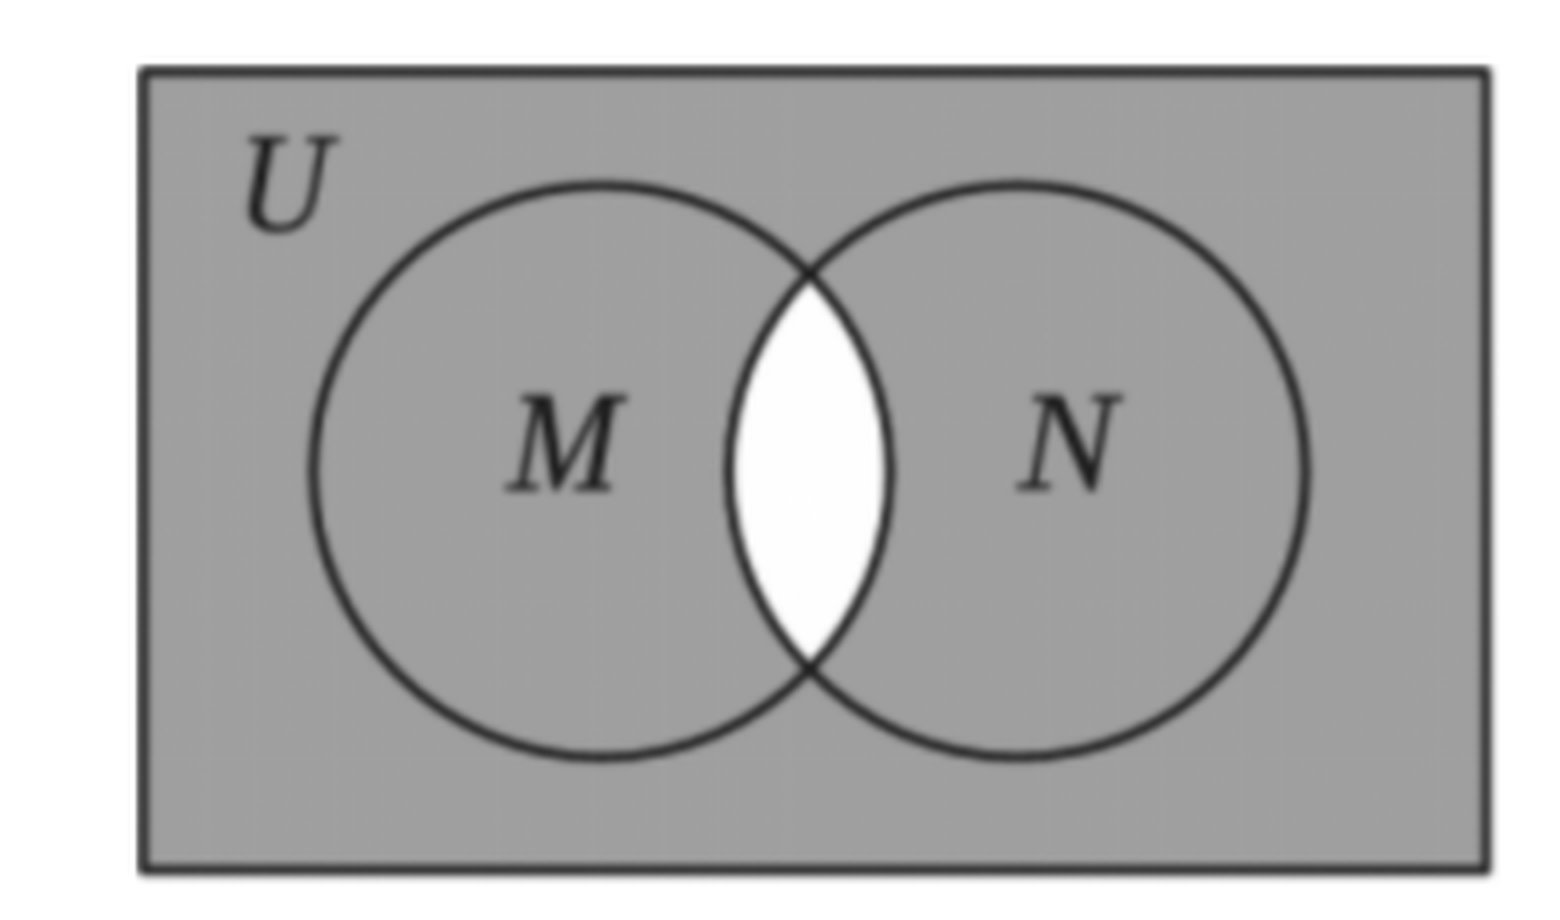
\includegraphics[width=0.40\textwidth]{figures/gao145_q14.png}
\end{center}

\ifanswer
\solbegin
\step{由韦恩图得图中白色区域为集合 $M\cap N$，所以阴影部分表示的集合为 $\overline{M\cap N}$.}
\step{故选 $D$.}
\solend
\fi

% === Q15 ===
\item 已知 $x>-2$，则 $x+\dfrac{1}{x+2}$ 的最小值为\mbox{（\quad）}

\keepwithprev
A. 3\qquad B. 2\qquad C. 1\qquad D. 0

\ifanswer
\solbegin
\step{$x>-2$，则 $x+2>0$，}
\step{所以 $x+\dfrac{1}{x+2}=(x+2)+\dfrac{1}{x+2}-2\geqslant2\sqrt{(x+2)\cdot\dfrac{1}{x+2}}-2=0$，}
\step{当且仅当 $x+2=\dfrac{1}{x+2}$，即 $x=-1$ 时取等号，所以 $x+\dfrac{1}{x+2}$ 的最小值为 $0$.}
\step{故选 $D$.}
\solend
\fi

% 第 16 题：题干在 05 页、解析续至 06 页；两幅数轴标根波浪曲线是【解析】内配图，
% 仅答案版出，放在答案版条件块内 \solbegin 的 \step 之间（照 高一73 第 16 题成例）
\item 关于 $x$ 的不等式 $\dfrac{(x-a)(x-2)^2}{(x-1)(x-5)}\leqslant0$ 的解集中恰有 3 个正整数，则实数 $a$ 的取值范围是\mbox{（\quad）}

\keepwithprev
A. $(-\infty,3]\cup[7,8)$\qquad B. $(-\infty,3)\cup[7,8)$\qquad C. $(-\infty,3]\cup(7,8]$\qquad D. $(-\infty,3)\cup(7,8]$

\ifanswer
\solbegin
\step{由题意，不等式 $\dfrac{(x-a)(x-2)^2}{(x-1)(x-5)}\leqslant0$，}
\step{可化为 $\begin{cases}(x-1)(x-2)^2(x-5)(x-a)\leqslant0\\x\ne1\text{且}x\ne5\end{cases}$，由数轴标根法，}
\step{当 $a=3$ 时，}
\begin{center}
% a=3 数轴标根图取 06 页，去粉色水印、去色、4× LANCZOS 放大；仅答案版出
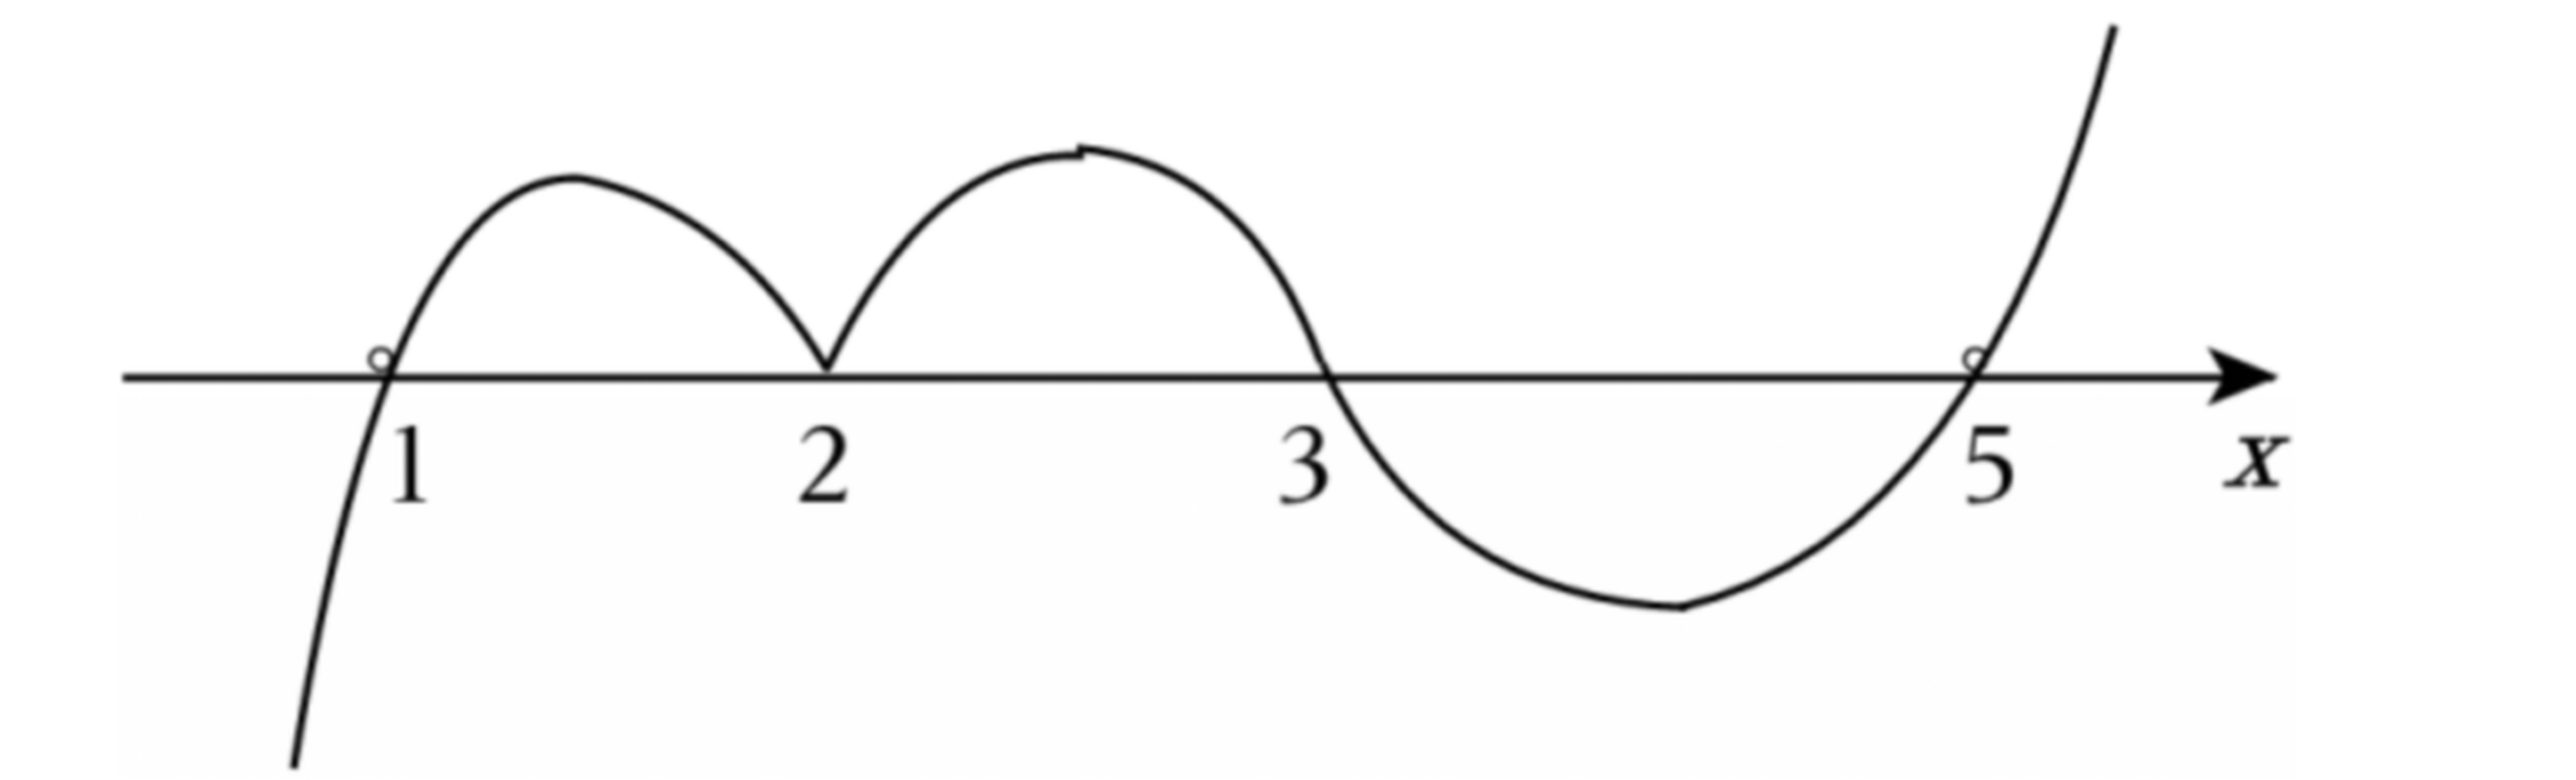
\includegraphics[width=0.62\textwidth]{figures/gao145_q16_a3.png}
\end{center}
\step{得不等式的解集为 $\{x\mid x<1\text{ 或 }x=2\text{ 或 }3\leqslant x<5\}$，}
\step{对应的正整数解为 $2$，$3$，$4$，满足题意，故排除 $B$、$D$；}
\step{当 $a=7$ 时，}
\begin{center}
% a=7 数轴标根图取 06 页，去粉色水印、去色、4× LANCZOS 放大；仅答案版出
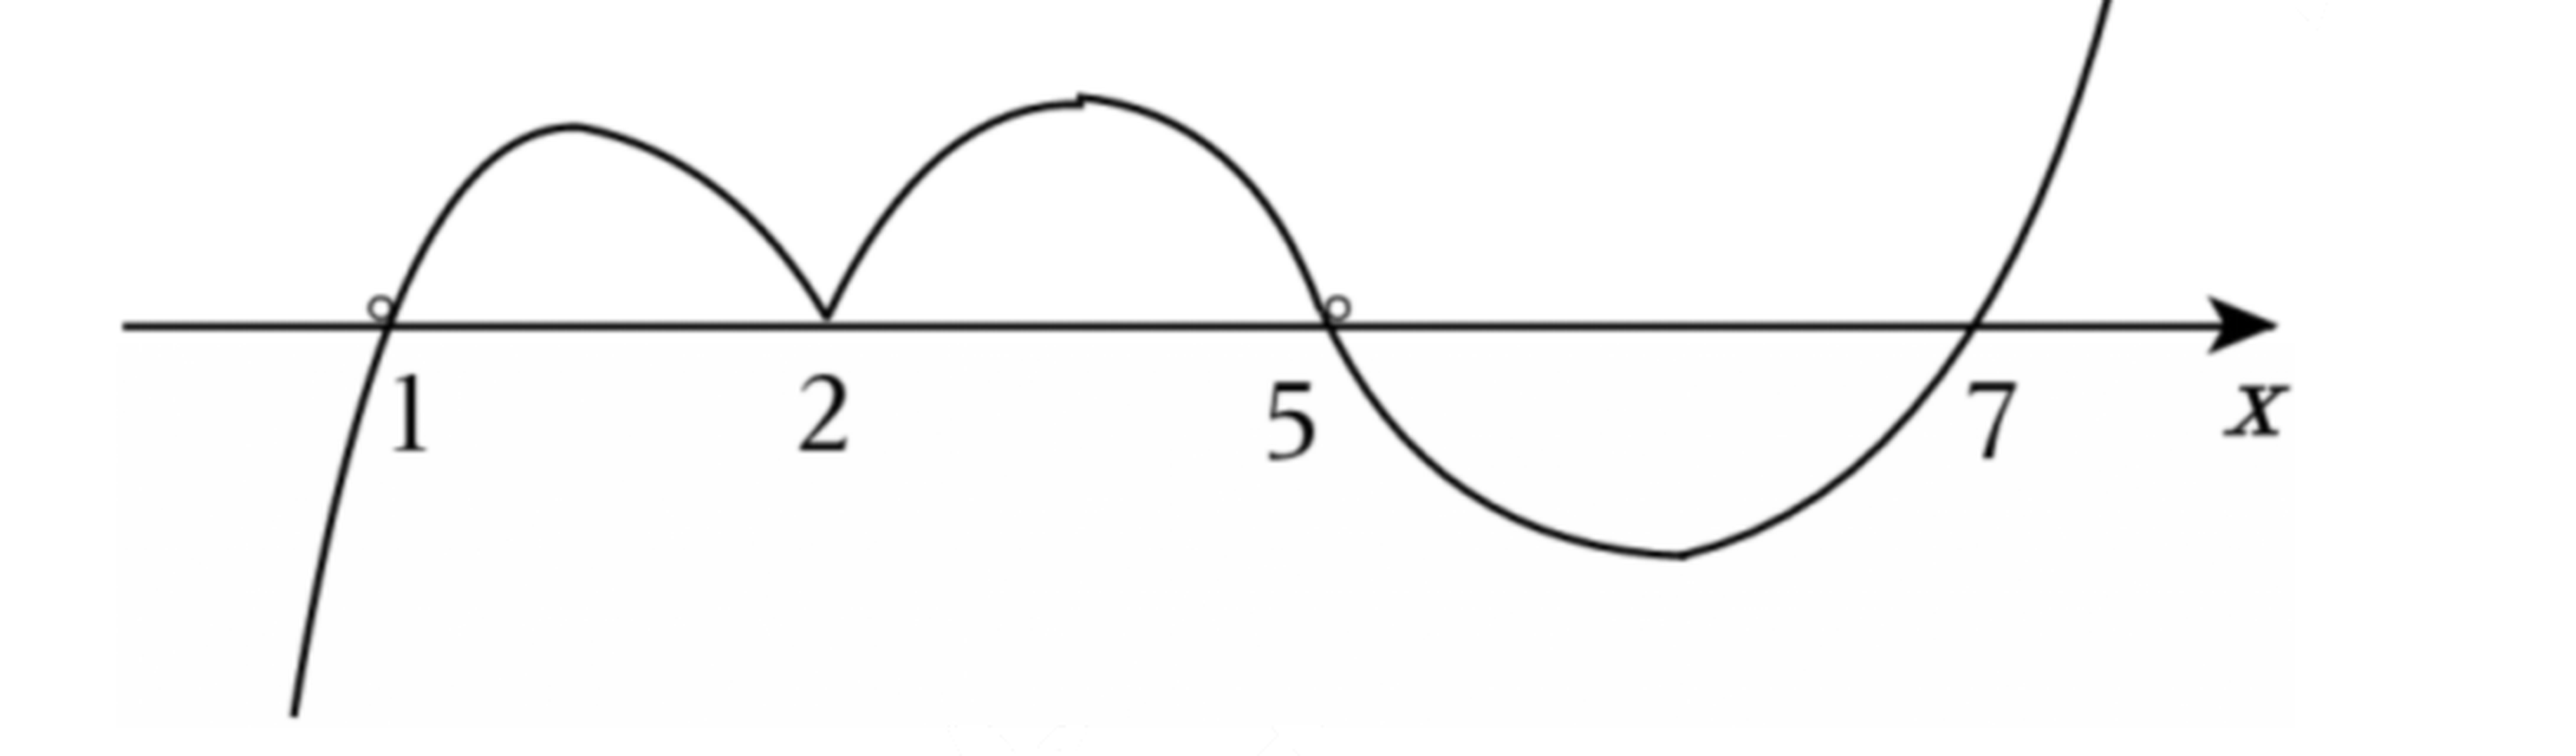
\includegraphics[width=0.62\textwidth]{figures/gao145_q16_a7.png}
\end{center}
\step{得不等式的解集为 $\{x\mid x<1\text{ 或 }x=2\text{ 或 }5<x\leqslant7\}$，}
\step{对应的正整数解为 $2$，$6$，$7$，满足题意，故 $A$ 正确，$C$ 错误.}
\step{故选 $A$.}
\solend
\fi

\end{enumerate}

\bigsec{三、解答题}

\begin{enumerate}
\setcounter{enumi}{16}

% 第 17 题：题干在 06 页、解析续至 07 页，按印刷行断，共 7 行；
% "lg(10÷5)" 的除号照录 \div
\item (1) 已知 $a+a^{-1}=6$，求 $a^2+a^{-2}$ 及 $a^{\frac12}-a^{-\frac12}$ 的值；

(2) 已知 $\lg5=a$，$\lg6=b$，用 $a$、$b$ 分别表示 $\lg2$、$\lg3$、$\lg300$ 和 $\log_{12}15$.

\ifanswer
\solbegin
\step{(1) 因为 $a+a^{-1}=6$，}
\step{所以 $a^2+a^{-2}=(a+a^{-1})^2-2\cdot a\cdot a^{-1}=6^2-2=34$，}
\step{因为 $\left(a^{\frac12}-a^{-\frac12}\right)^2=a-2+a^{-1}=6-2=4$，所以 $a^{\frac12}-a^{-\frac12}=\pm2$；}
\step{(2) $\lg2=\lg(10\div5)=\lg10-\lg5=1-a$，}
\step{$\lg3=\lg(6\div2)=\lg6-\lg2=b-(1-a)=a+b-1$，}
\step{$\lg300=\lg(3\times10^2)=\lg3+\lg10^2=a+b-1+2=a+b+1$，}
\step{所以 $\log_{12}15=\dfrac{\lg15}{\lg12}=\dfrac{\lg3+\lg5}{\lg3+\lg2^2}=\dfrac{a+b-1+a}{a+b-1+2(1-a)}=\dfrac{2a+b-1}{b-a+1}$.}
\solend
\fi

% 第 18 题：题干在 07 页、解析续至 08 页（2 问、分类讨论很长），按印刷行断共 25 行；
% 本卷 Q18 用"图像"（Q13/Q14 用"图象"），逐处照录不统一
\item 已知 $f(x)=(m^2-3m+1)x^{m^2-4m-1}$，$y=f(x)$ 为幂函数且在 $(0,+\infty)$ 上是严格减函数.

(1) 求实数 $m$ 的值以及相应的函数表达式；

(2) 若 $y=f(x)$ 的图像关于 $y$ 轴对称，解关于 $x$ 的不等式 $(x+2)^{1-m}<(3x-1)^{1-m}$.

\ifanswer
\solbegin
\step{(1) 由幂函数的定义得 $m^2-3m+1=1$，}
\step{整理得 $m^2-3m=0$，解得 $m=0$ 或 $m=3$，}
\step{由于 $y=f(x)$ 在 $(0,+\infty)$ 上为严格减函数，}
\step{因此幂函数的指数需满足 $m^2-4m-1<0$，}
\step{当 $m=3$ 时，指数为 $3^2-4\times3-1=-4<0$，满足严格递减条件，}
\step{此时函数表达式为 $f(x)=x^{-4}$，}
\step{当 $m=0$ 时，指数为 $0^2-4\times0-1=-1<0$，满足严格递减条件，}
\step{此时函数表达式为 $f(x)=x^{-1}$，}
\step{所以满足条件的实数 $m$ 为 $0$ 或 $3$，}
\step{对应的函数表达式分别为 $f(x)=x^{-1}$、$f(x)=x^{-4}$；}
\step{(2) 函数图像关于 $y$ 轴对称即函数为偶函数，}
\step{对于 $f(x)=x^{-1}=\dfrac1x$，定义域为 $(-\infty,0)\cup(0,+\infty)$，}
\step{满足 $f(-x)=-f(x)$，为奇函数，图像关于原点对称，}
\step{不满足关于 $y$ 轴对称的条件；}
\step{对于 $f(x)=x^{-4}=\dfrac{1}{x^4}$，定义域为 $(-\infty,0)\cup(0,+\infty)$，}
\step{满足 $f(-x)=f(x)$，为偶函数，图像关于 $y$ 轴对称，}
\step{因此符合条件的 $m$ 值为 $3$，}
\step{将 $m=3$ 代入关于 $x$ 的不等式 $(x+2)^{1-m}<(3x-1)^{1-m}$，}
\step{得 $(x+2)^{1-3}<(3x-1)^{1-3}$，即 $(x+2)^{-2}<(3x-1)^{-2}$，}
\step{因为负指数幂的底数不能为 $0$，所以 $x+2\ne0$ 且 $3x-1\ne0$，}
\step{即 $x\ne-2$ 且 $x\ne\dfrac13$，}
\step{不等式可变形为 $\dfrac{1}{(x+2)^2}<\dfrac{1}{(3x-1)^2}$，}
\step{整理得 $(3x-1)^2<(x+2)^2$，即 $8x^2-10x-3<0$，}
\step{解得 $-\dfrac14<x<\dfrac32$，又 $x\ne-2$ 且 $x\ne\dfrac13$，}
\step{所以不等式的解集为 $\left(-\dfrac14,\dfrac13\right)\cup\left(\dfrac13,\dfrac32\right)$.}
\solend
\fi

% 第 19 题：题干在 08 页、解析续至 09 页，按印刷行断，共 14 行；
% 判别式 cases 块内"△=4a²−16a<0"原卷印扁等边三角 \triangle
%（放大 09 页 zz09_delta.png 与 Q12 高 \Delta 并排确认），逐处照录不统一
\item 已知 $f(x)=ax^2+2ax+4$，$a\in\R$.

(1) 若关于 $x$ 的不等式 $f(x)>0$ 在实数集 $\R$ 上恒成立，求实数 $a$ 的取值范围；

(2) 当 $a<0$ 时，解关于 $x$ 的不等式 $f(x)>(a+1)x+5$.

\ifanswer
\solbegin
\step{(1) 由题意得，关于 $x$ 的不等式 $f(x)>0$ 在实数集 $\R$ 上恒成立，}
\step{即 $ax^2+2ax+4>0$ 在实数集 $\R$ 上恒成立，}
\step{当 $a=0$ 时，不等式为 $4>0$ 恒成立，符合题意；}
\step{当 $a\ne0$ 时，则 $\begin{cases}a>0\\\triangle=4a^2-16a<0\end{cases}$，解得 $0<a<4$.}% 判别式原卷印扁等边三角 $\triangle$，照录
\step{综上所述，实数 $a$ 的取值范围为 $[0,4)$.}
\step{(2) $f(x)=ax^2+2ax+4$，}
\step{当 $a<0$ 时，不等式 $f(x)>(a+1)x+5$ 即为 $ax^2+(a-1)x-1>0$，}
\step{即 $(ax-1)(x+1)>0$，即 $\left(x-\dfrac1a\right)(x+1)<0$，}
\step{当 $a<-1$，即 $\dfrac1a>-1$ 时，解得 $-1<x<\dfrac1a$；}
\step{当 $a=-1$，即 $\dfrac1a=-1$ 时，解得 $x\in\varnothing$；}
\step{当 $-1<a<0$，即 $\dfrac1a<-1$ 时，解得 $\dfrac1a<x<-1$.}
\step{综上所述，当 $a<-1$ 时，不等式的解集为 $\left\{x\mid -1<x<\dfrac1a\right\}$；}
\step{当 $a=-1$ 时，不等式的解集为 $\varnothing$；}
\step{当 $-1<a<0$ 时，不等式的解集为 $\left\{x\mid \dfrac1a<x<-1\right\}$.}
\solend
\fi

% 第 20 题：菜园靠墙图为题目配图（三版都出），题干写"如图"；
% 题干在 09 页（含图）、解析续至 10 页，按印刷行断，共 13 行
\needvspace{8cm}
\item 如图，某人计划用篱笆围成一个一边靠墙（墙足够长）的矩形菜园. 设菜园的长为 $x$ 米，宽为 $y$ 米.

\begin{center}
% 矩形菜园靠墙图取 09 页右下，去粉色水印、去色、4× LANCZOS 放大
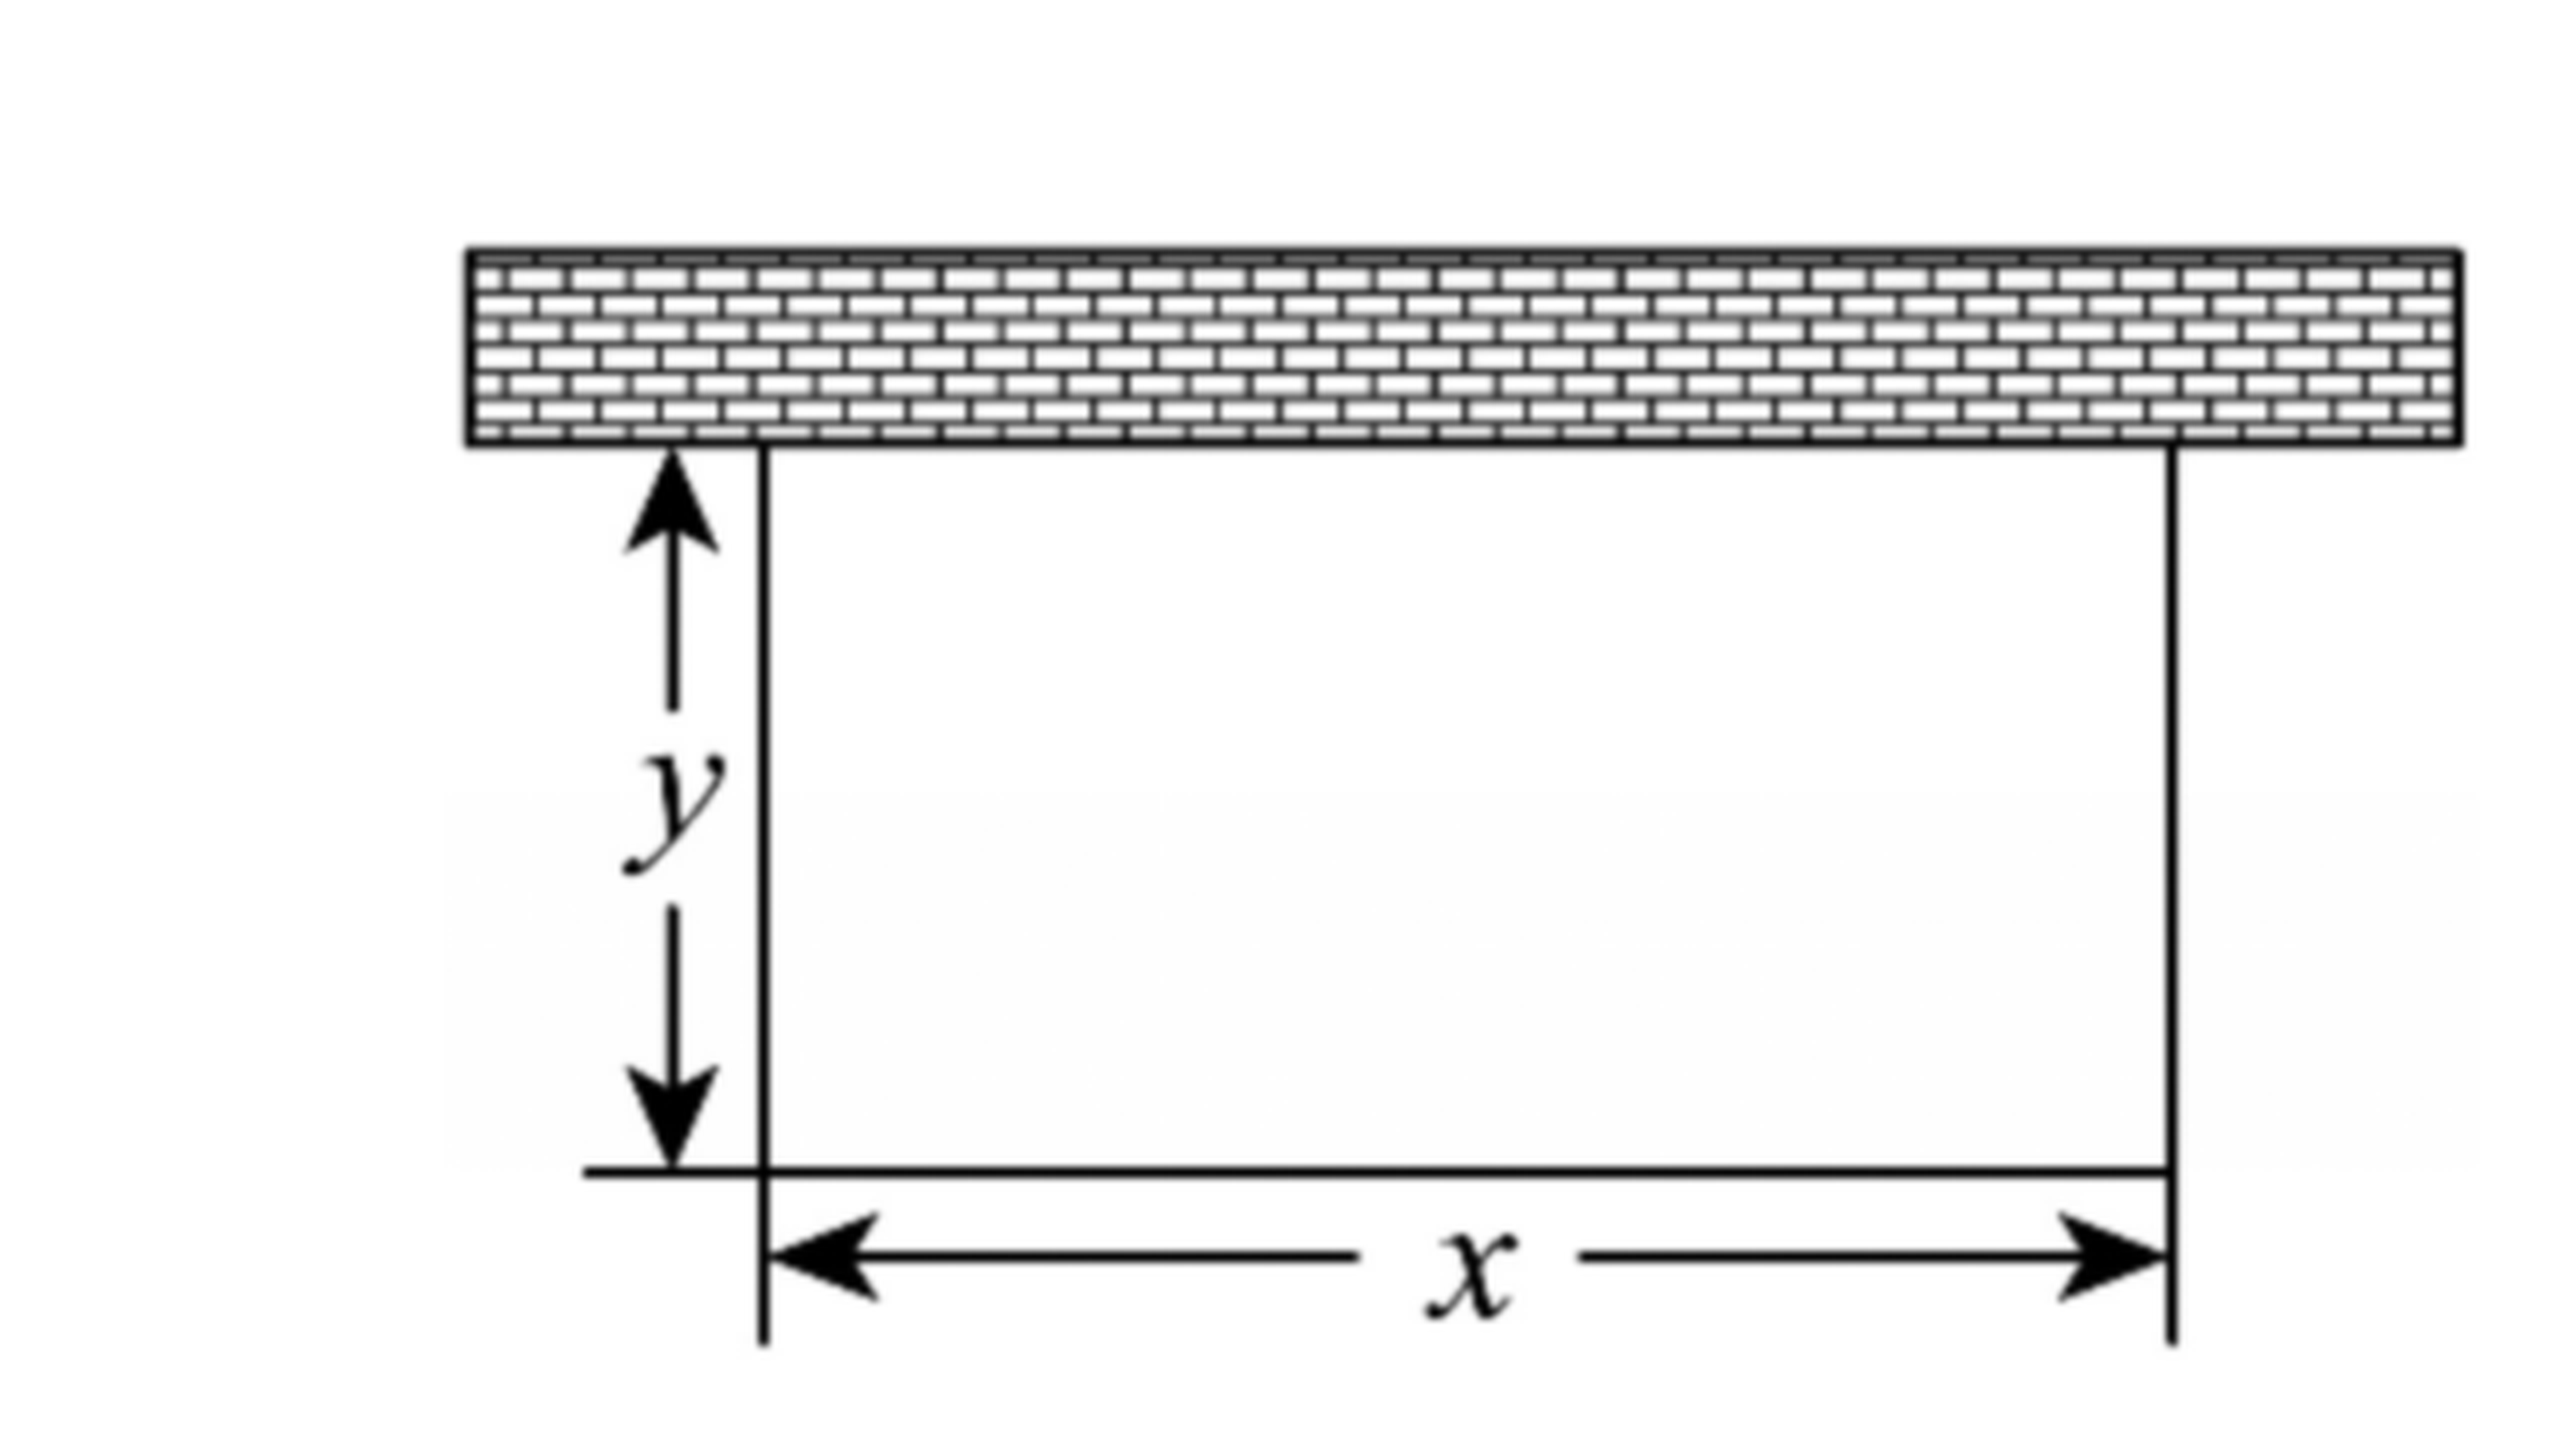
\includegraphics[width=0.55\textwidth]{figures/gao145_q20.png}
\end{center}

(1) 若菜园面积为 72 平方米，则 $x$、$y$ 为何值时，所用篱笆总长最小？

(2) 若 $x$、$y$ 满足 $x+y-xy+63=0$，则菜园面积最小为多少平方米？

\ifanswer
\solbegin
\step{(1) 由题意得，菜园的面积 $S=xy=72$，且 $x>0$，$y>0$，}
\step{所用篱笆总长 $L=x+2y$，}
\step{由基本不等式得 $x+2y\geqslant2\sqrt{x\cdot2y}=2\sqrt{2xy}=2\sqrt{2\times72}=24$，}
\step{当且仅当 $x=2y$ 时取等号，}
\step{联立 $\begin{cases}xy=72\\x=2y\end{cases}$，解得 $\begin{cases}x=12\\y=6\end{cases}$，}
\step{所以当 $x=12$，$y=6$ 时，所用篱笆总长最小；}
\step{(2) 由题意得 $x>0$，$y>0$，且满足 $x+y-xy+63=0$，即 $x+y=xy-63$，}
\step{由基本不等式得 $x+y\geqslant2\sqrt{xy}$，当且仅当 $x=y$ 时取等号，}
\step{所以 $xy-63\geqslant2\sqrt{xy}$. 令 $t=\sqrt{xy}(t>0)$，则 $xy=t^2$，}
\step{上述不等式可化为 $t^2-2t-63\geqslant0$，即 $(t-9)(t+7)\geqslant0$，}
\step{因为 $t>0$，所以 $t+7>0$，故 $t-9\geqslant0$，解得 $t\geqslant9$，所以 $\sqrt{xy}\geqslant9$，}
\step{即 $xy\geqslant81$，当且仅当 $x=y=9$ 时取等号，此时满足 $9+9-81+63=0$，}
\step{所以菜园面积最小为 81 平方米.}
\solend
\fi

% 第 21 题：题干在 10 页、解析续至 11 页（3 问、分类讨论很长），按印刷行断共 22 行；
% 末行"故第 2026 个元素是 2700 之后第一个属于 A 的数，即 2701." 为全卷收尾，
% 无 Q22/Q23、无附加题节；数集 Z/N* 按全稿惯例改 \Z/\N^*
\item 已知集合 $A=\{x\mid x=m^2-n^2$，$m$、$n\in\Z\}$.

(1) 求证：任何奇数 $2k+1(k\in\Z)$ 都是集合 $A$ 中的元素；

(2) 判断偶数 $4k-2(k\in\Z)$ 是否为集合 $A$ 的元素？请说明理由；

(3) 若将集合 $A$ 中的正整数由小到大排列，求出集合 $A$ 中第 2026 个正整数.

\ifanswer
\solbegin
\step{(1) 因为 $x=(k+1)^2-k^2=2k+1(k\in\Z)$，}
\step{所以任何奇数 $2k+1(k\in\Z)$ 都属于集合 $A$；}
\step{(2) 偶数 $4k-2(k\in\Z)$ 不是集合 $A$ 的元素，理由如下：}
\step{由题意得 $x=m^2-n^2=(m-n)(m+n)$，}
\step{当 $m$、$n$ 均为奇数时，设 $m=2k_1+1$，$n=2k_2+1(k_1$、$k_2\in\Z)$，}
\step{则 $m^2-n^2=(2k_1+1)^2-(2k_2+1)^2=(2k_1-2k_2)(2k_1+2k_2+2)$}
\step{$=4(k_1-k_2)(k_1+k_2+1)$，}
\step{因为 $k_1$、$k_2\in\Z$，所以 $k_1-k_2\in\Z$，$k_1+k_2+1\in\Z$，}
\step{从而 $m^2-n^2$ 为 $4$ 的倍数；}
\step{当 $m$、$n$ 均为偶数时，设 $m=2k_1$，$n=2k_2(k_1$、$k_2\in\Z)$，}
\step{$m^2-n^2=4k_1^2-4k_2^2=4(k_1^2-k_2^2)$ 为 $4$ 的倍数；}
\step{当 $m$、$n$ 为一个偶数一个奇数时，不妨设 $m$ 为偶数，$n$ 为奇数，}
\step{设 $m=2k_1$，$n=2k_2+1(k_1$、$k_2\in\Z)$，}
\step{则 $m^2-n^2=4k_1^2-(2k_2+1)^2=4(k_1^2-k_2^2-k_2)-1$ 为奇数.}
\step{无论哪种情况均不满足 $4k-2(k\in\Z)$，}
\step{故偶数 $4k-2(k\in\Z)$ 不是集合 $A$ 的元素；}
\step{(3) 由前两问得，$4$ 的倍数和奇数属于集合 $A$ 中的元素，}
\step{令集合 $A$ 中的正整数元素为 $4k-3$、$4k-1$、$4k(k\in\N^*)$，}
\step{对任意的 $k\in\N^*$，连续的 $4$ 个整数 $4k-3$、$4k-2$、$4k-1$、$4k$ 中}
\step{有三个数 $4k-3$、$4k-1$、$4k$ 都在集合 $A$ 中，}
\step{因为 $2026=3\times675+1$，所以集合 $A$ 中第 $2025$ 个元素为 $4\times675=2700$，}
\step{故第 2026 个元素是 2700 之后第一个属于 $A$ 的数，即 2701.}
\solend
\fi

\end{enumerate}

\end{document}
"
%
% ① 原始材料：微信公众号"魔都数学加油站"文章，连载"27学年高一145"，原文标题
% "27学年高一145——2026-2027年上海市市二中学高一上期中"；
% 原文链接：https://mp.weixin.qq.com/s/6V-i9KE0GWodC-wmd5z8nQ 。
% 正文为 11 张 PNG 页（01/02/03/08/10/11 为 4762×6735，04/05/06/07/09 为 2560×3620，
% 同一篇各页分辨率不同，逐页按各自分辨率裁图核对，别按预览比例换算裁框）。
% 题目下印【答案】或【解析】，为混合体例讲评版：Q3 只印【答案】、无【解析】，其余
% 18 题印【解析】。题目、解析均据原图转录；卷面粉红色水印"魔都数学加油站"及
% 公众号页脚未录入。
% 全卷插图情况（逐页通读 11 页确认，题干写"如图"处均配有图）：
%   · Q14 韦恩图（05 页右侧，全集 U 矩形＋两圆 M/N＋白色交集、灰色阴影＋U/M/N 标注）：
%     题目配图（选择题选项旁），三版都出，裁自 05 页去水印去色 4× 放大存
%     figures/gao145_q14.png；
%   · Q16 两幅数轴标根波浪曲线（06 页，a=3 与 a=7 各一幅，标根法画
%     (x-1)(x-2)^2(x-5)(x-a)≤0 的符号曲线）：【解析】内的配图，仅答案版出，
%     裁 figures/gao145_q16_a3.png / figures/gao145_q16_a7.png（或合并一张），
%     放在答案版条件块内 \solbegin 的 \step 之间（照 高一73 第 16 题成例）；
%   · Q20 矩形菜园靠墙图（09 页右下，灰色砖墙＋矩形菜园＋x/y 标注＋箭头）：
%     题目配图，三版都出，裁自 09 页去水印去色 4× 放大存 figures/gao145_q20.png；
%   其余各页逐页确认无其它题目配图、无表格、亦无"题干写如图而源码漏图"一处。
%
% 卷首标题：原卷印作"2026-2027 年市二中学高一上期中"，年份区间按全稿惯例排 en dash；
% 原卷卷面未印副标题，本稿按同期中卷（高一140／141／143／144）知识模块口径补出
% "集合与常用逻辑用语、不等式、函数"。
%
% 题号体例：本卷共 19 题——一、填空题 3—12（10 题）、二、选择题 13—16（4 题）、
% 三、解答题 17—21（5 题）。三节分别 \setcounter{enumi}{2}／{12}／{16}。
% 原卷从第 3 题起、无第 1、2 题，本稿保留原题号；全卷无附加题节。
%
% ② 与原卷的排版差异：
%   ① 原文从第 3 题起，本稿保留原题号；共 19 题三节；
%   ② 混合体例：原卷 Q3 只印【答案】、无【解析】（"第一步应假设___。
%      【答案】x≤2 或 y≤2"），按 高一140 第 5 题成例提 \ans{}、不补造解析；
%      其余 18 题印【解析】，用 \solbegin…\solend，选择题答案在解析末句"故选 X"
%      （Q13 选 B、Q14 选 D、Q15 选 D、Q16 选 A，逐个放大原图核实）、
%      题干括号 \mbox{（\quad）} 留空、不另提 \ans{}；填空／解答答案落在解析里；
%      答案版【答案】/【解析】标记数 = 19（1 个 \ans ＋ 18 个 \solbegin）= 全卷题数；
%   ③ 原卷卷面未印副标题，本稿按知识模块口径补出；
%   ④ 原卷填空横线按全稿惯例排 \blankline[4.4em]；选择题括号排 \mbox{（\quad）}、
%      选项段前按惯例加 \keepwithprev；解答题不留作答区、不加 \anspace
%      （原卷为讲评版，与 129／131／132／133／136／140／141／143／144 同）；
%   ⑤ 数集：Q9"a、b∈R"、Q12"a∈R"、Q21"m、n∈Z""k∈Z""k∈N*"等原卷印
%      斜体或黑板粗体 R/Z/N，按全稿惯例统一改 \R／\Z／\N^*；绝对值排 \lvert…\rvert，
%      集合描述竖线排 \mid；不等号按全稿惯例排 \leqslant／\geqslant；
%      补集照原卷上划线排 \overline{M}／\overline{N}（Q14 选项 B/C/D 逐处核）；
%      空集记号 \varnothing；\subset（单线⊂）与 \subseteq（带下划线⊆）逐处照录不统一；
%   ⑥ 子题标号 (1)(2)(3) 原卷印半角括号照录；圈数字进数学式用 \text{①}（否则 FONTCHK 挂）；
%      \left…\right 不得拆到不同 $…$ 组；cases 块整体算一个印刷行；
%   ⑦ 题干／解析中的中文弯引号按原卷照录（Q3"若 x+y>4，则 x>2 且 y>2"、
%      Q11"a₁/a₂=b₁/b₂""M=N"、选填"充分非必要""必要非充分""充要""既非充分也非必要"
%      等，含引号内空格），注释内一律 ASCII 引号；数学式内 CJK 用 \text{}；
%   ⑧ 半角逗号在数学组之间是全稿惯例、非笔误（如 Q5"x₁+x₂=6，x₁x₂=√3"、
%      Q7"a>1，b>1"、指数／对数式内逗号），逐处照录别改全角；行末西文句点照录为
%      ASCII `.`；行中全角逗号／顿号照录；
%   ⑨ "图像／图象"逐处照录不统一（Q18"图像关于 y 轴对称"等，核全卷）；
%   ⑩ 判别式 Δ/△ 混用是照录项：Q12 解析"Δ=a²−4a²(2a−3)>0"、
%      Q19 解析"Δ=4a²−16a<0"等，放大原图判断是高 \Delta（等腰偏高、高>宽）
%      还是扁 \triangle，逐处照录不得统一（参照 高一142／144 头注④口径）；
%   ⑪ 一条 \step = 原卷解析的一个印刷行，cases 块整体算一个印刷行；别把原卷折行
%      并起来、别把一行拆多条。Q6 分段讨论、Q12 三个 cases 条件组、Q16 数轴标根、
%      Q18／Q19 分类讨论、Q21 三问均按印刷行逐条断，不丢行；
%   ⑫ Q14 韦恩图为"题干＋选项＋图"整块，加 \needvspace 守卫推走（守卫放 \item 之前，
%      见 高一140 Q14、高一144 Q17 成例与切页审计 B 类坑）；Q20 菜园图同理；
%      三版切页审计均"合计异常：无"；
%   ⑬ 跨页续印按题合并：Q3/4/5/6 在 01 页（Q6 解析续 02 页顶）；Q7/8/9/10 在 02 页
%      （Q10 解析续 03 页）；Q11/12 在 03 页（Q12 解析续 04 页，很长）；
%      Q13 在 04 页末、解析在 05 页顶；Q14/15/16 在 05 页（Q16 解析续 06 页含两幅数轴图）；
%      Q17 在 06 页、解析续 07 页；Q18 在 07 页、解析续 08 页；Q19 在 08 页、解析续 09 页；
%      Q20 在 09 页（含菜园图）、解析续 10 页；Q21 在 10 页、解析续 11 页
%      （末页收尾"故第 2026 个元素是 2700 之后第一个属于 A 的数，即 2701."、
%      无 Q22/Q23、无附加题节）。本稿按题连排，不丢行、不并折行；
%   ⑭ 原卷解析内若有红色"法一／法二"之类小标题，按全稿惯例排 \stepm{标签}{…}
%      （黑体着色、不引入红色、不改 common.sty），头注注明；水印"魔都数学加油站"
%      红色不录入。
%
% ③ 行数复核：一条 \step／\stepm = 原卷解析的一个印刷行，cases 块作一个印刷行计。
%   逐题数（主会话逐页核对定稿）：Q3：0（只印【答案】、提 \ans{}，不计入 \step 账）；
%   Q4：3；Q5：2；Q6：10；Q7：3；Q8：3；Q9：2；Q10：7；Q11：4；Q12：12；
%   Q13：2；Q14：2；Q15：4；Q16：9；Q17：7；Q18：25；Q19：14；Q20：13；Q21：22。
%   合计 144 条 \step（本卷无 \stepm：解析内无红色"法一／法二"类小标题），
%   与原卷逐题印刷行相等。全卷 18 题设 \solbegin…\solend ＋ Q3 一处 \ans{}，
%   答案版【答案】/【解析】标记数 = 19 = 全卷题数。
%
% ④ 判别式／子集符号结论（逐处放大原图照录、不得统一，主会话像素级复核）：
%   判别式全卷 2 处、两形混用逐处照录不统一（参照 高一142／144 头注④口径）：
%     · Q12 解析 cases 块"Δ=a²−4a²(2a−3)>0" 原卷印等腰偏高粗三角（高>宽），
%       照录 \Delta（放大 04 页 /tmp/gao145s2/main_q12_delta.png 确认）；
%     · Q19 解析 cases 块"△=4a²−16a<0" 原卷印扁等边空心三角（宽≈高、细线），
%       照录 \triangle（放大 09 页 /tmp/gao145s2/main_q19_delta.png 确认）。
%   子集／补集：Q14 选项 A `M\cup N`、B `M\cap\overline{N}`（上划线只在 N 上）、
%   C `\overline{M\cup N}`（罩整个 M∪N）、D `\overline{M\cap N}`（罩整个 M∩N，
%   非 \overline{M}\cap N；放大 05 页 /tmp/gao145s2/main_q14_opts.png 确认），
%   阴影为灰色区域＝全集减白色交集，答案 D，照录 \overline{M\cap N}；
%   全集卷无 \subset／\subseteq 混用（本卷集合题用 \cup／\cap／\overline{}）；
%   空集 \varnothing（Q19 解析 x∈\varnothing）；数集 \R／\Z／\N^* 归一见 ② ⑤。
%
% ⑤ 存疑照录（放大原图确认，照录未改、正文对应处另有 % 注）：
%   1. Q3 题干"若 x+y>4，则 x>2 且 y>2" 后"时"前留一空格、弯引号内空格照录；
%      该卷混合体例（Q3 只印【答案】、提 \ans{}）见 ② ②。
%   2. Q4／Q5 解析中的"1，3，5 和 6"、"x₁+x₂=6,x₁x₂=√3" 等半角／全角逗号
%      逐处照原卷（放大 01 页确认），数学式内半角逗号为全稿惯例、非笔误。
%   3. Q14 选项 D 上划线罩住整个 M∩N（而非仅罩 M），照录 \overline{M\cap N}。
%   4. Q12 判别式高 \Delta 与 Q19 判别式扁 \triangle 两形混用，逐处照录不统一（见 ④）。
%   全卷除此 4 类外未发现其它笔误／自相矛盾处。
%
% ⑥ 跨页续印按题合并说明：见 ② ⑬。
%
\documentclass[a4paper,11pt]{article}
\usepackage{common}

\begin{document}

\examtitlest[3]{2026--2027 年市二中学高一上期中}{集合与常用逻辑用语、不等式、函数}

\bigsec{一、填空题}

\begin{enumerate}
\setcounter{enumi}{2}

% 第 3 题：原卷只印【答案】、无【解析】（放大 01 页确认），按 高一140 第 5 题成例
% 提 \ans{}、不补造解析；题干中文弯引号与"时"前空格照录
\item 用反证法证明命题：“若 $x+y>4$，则 $x>2$ 且 $y>2$” 时，第一步应假设\blankline[4.4em].

\ifanswer
\ans{$x\leqslant2$ 或 $y\leqslant2$}
\fi

% === Q4 ===
\item 设集合 $M$ 满足 $\{1,3,5,6\}\cup M=\{1,2,3,4,5,6\}$，则满足条件的所有 $M$ 的个数为\blankline[4.4em].

\ifanswer
\solbegin
\step{集合 $M$ 满足 $\{1,3,5,6\}\cup M=\{1,2,3,4,5,6\}$，}
\step{则 $M$ 中必含有 $2$ 和 $4$，$1$，$3$，$5$ 和 $6$ 可以选也可不选，}
\step{则满足条件的所有 $M$ 的数目相当于集合 $\{1,3,5,6\}$ 的子集的个数 $2^4=16$.}
\solend
\fi

% === Q5 ===
\item 已知方程 $x^2-6x+\sqrt3=0$ 的两根为 $x_1$ 和 $x_2$，则 $(x_1-x_2)^2=$\blankline[4.4em].

\ifanswer
\solbegin
\step{因为方程 $x^2-6x+\sqrt3=0$ 的两根为 $x_1$ 和 $x_2$，所以 $x_1+x_2=6,x_1x_2=\sqrt3$，}% 数学式内半角逗号为全稿惯例，照录
\step{所以 $(x_1-x_2)^2=(x_1+x_2)^2-4x_1x_2=36-4\sqrt3$.}
\solend
\fi

% 第 6 题：题干在 01 页，解析续至 02 页顶（末 2 行），按印刷行逐条断，共 10 行
\item 不等式 $\lvert x-2026\rvert+\lvert x-2029\rvert>3$ 的解集是\blankline[4.4em].

\ifanswer
\solbegin
\step{当 $x<2026$ 时，$x-2026<0$，$x-2029<0$，}
\step{原不等式可化为 $(2026-x)+(2029-x)>3$，解得 $x<2026$，}
\step{故此时，不等式的解为 $x<2026$；}
\step{当 $2026\leqslant x\leqslant2029$ 时，$x-2026\geqslant0$，$x-2029\leqslant0$，}
\step{原不等式可化为 $(x-2026)+(2029-x)>3$，即 $3>3$，显然不成立，}
\step{故此时，不等式无解；}
\step{当 $x>2029$ 时，$x-2026>0$，$x-2029>0$，}
\step{原不等式可化为 $(x-2026)+(x-2029)>3$，解得 $x>2029$，}
\step{故此时，不等式的解为 $x>2029$.}
\step{综上，原不等式的解集为 $(-\infty,2026)\cup(2029,+\infty)$.}
\solend
\fi

% === Q7 ===
\item 已知 $a>1$，$b>1$，若 $\log_a b+\log_b a=2$，且 $ab=2$，则 $\log_2(a+b)=$\blankline[4.4em].

\ifanswer
\solbegin
\step{由 $\log_a b+\log_b a=2$，$a>1$，$b>1$，得 $\log_a b+\dfrac{1}{\log_a b}=2$，}
\step{即 $(\log_a b)^2-2\log_a b+1=0$，则 $(\log_a b-1)^2=0$，解得 $\log_a b=1$，即 $a=b$，}
\step{又 $ab=2$，所以 $a=b=\sqrt2$，所以 $\log_2(a+b)=\log_2 2\sqrt2=\log_2 2^{\frac32}=\dfrac32$.}
\solend
\fi

% === Q8 ===
\item 已知 $m>0$，$n>0$，且 $m+n=1$，则 $\dfrac1m+\dfrac4n$ 的最小值为\blankline[4.4em].

\ifanswer
\solbegin
\step{由 $m>0$，$n>0$，$m+n=1$，}
\step{则 $\dfrac1m+\dfrac4n=(m+n)\left(\dfrac1m+\dfrac4n\right)=5+\dfrac nm+\dfrac{4m}n\geqslant5+2\sqrt{\dfrac nm\cdot\dfrac{4m}n}=9$，}
\step{当且仅当 $n=2m=\dfrac23$ 时，上式取得等号，故最小值为 $9$.}
\solend
\fi

% === Q9 ===
\item 已知 $a$、$b\in\R$，且 $3a+2b=1$，则 $8^a+4^b$ 最小值为\blankline[4.4em].

\ifanswer
\solbegin
\step{因为 $3a+2b=1$，所以 $8^a+4^b=2^{3a}+2^{2b}\geqslant2\sqrt{2^{3a+2b}}=2\sqrt2$，}
\step{当且仅当 $3a=2b$ 时取等号，故最小值为 $2\sqrt2$.}
\solend
\fi

% 第 10 题：题干在 02 页、解析续至 03 页顶，按印刷行断，共 7 行
\item 已知关于 $x$ 的不等式 $ax^2+bx+c>0$ 的解集为 $\{x\mid 1<x<2\}$，则关于 $x$ 的不等式 $bx^2-ax+c<0$ 的解集为\blankline[4.4em].

\ifanswer
\solbegin
\step{已知关于 $x$ 的不等式 $ax^2+bx+c>0$ 的解集为 $\{x\mid 1<x<2\}$，}
\step{由解集为 $1<x<2$ 且二次函数在两根之间为正，得 $a<0$，两个根为 $1$，$2$，}
\step{所以 $ax^2+bx+c=a(x-1)(x-2)=ax^2-3ax+2a$，}
\step{比较系数得 $b=-3a$，$c=2a$.}
\step{于是 $bx^2-ax+c=-3ax^2-ax+2a=-a(3x-2)(x+1)$，}
\step{$a<0$，故 $bx^2-ax+c<0$ 等价于 $(3x-2)(x+1)<0$，解得 $-1<x<\dfrac23$，}
\step{故 $bx^2-ax+c<0$ 的解集为 $\left\{x\mid -1<x<\dfrac23\right\}$.}
\solend
\fi

% 第 11 题：题干引号内空格照录（放大 03 页确认），四组选填引号亦同；
% 结论"故为必要非充分条件"照录，解析共 4 个印刷行
\item 设 $a_1$、$b_1$、$a_2$、$b_2$ 均为非零实数，不等式 $a_1x+b_1>0$ 和 $a_2x+b_2>0$ 的解集分别为集合 $M$、$N$，那么 “ $\dfrac{a_1}{a_2}=\dfrac{b_1}{b_2}$ ” 是 “ $M=N$ ” 的\blankline[4.4em]条件（选填 “ 充分非必要 ”、“ 必要非充分 ”、“ 充要 ” 和 “ 既非充分也非必要 ”）.

\ifanswer
\solbegin
\step{当 $a_1=b_1=1$，$a_2=b_2=-1$ 时，满足 $\dfrac{a_1}{a_2}=\dfrac{b_1}{b_2}$，}
\step{但是 $M=N$ 不成立，即充分性不成立；}
\step{若 $M=N$ 时，$\dfrac{a_1}{a_2}=\dfrac{b_1}{b_2}$ 一定成立，即必要性成立.}
\step{故为必要非充分条件.}
\solend
\fi

% 第 12 题：题干在 03 页、解析续至 04 页（很长，含 3 个 cases 条件组），
% 按印刷行逐条断共 12 行；cases 块整体算一个印刷行
\item 已知 $f(x)=\dfrac{ax+3}{x-2}$（常数 $a\in\R$）. 函数 $y=f(x)$ 在区间 $[3,+\infty)$ 上是严格减函数，且函数值不恒为负. 若关于 $x$ 的方程 $f(x)=\dfrac{a}{ax-1}$ 有两个不相等的实数根 $x_1$ 和 $x_2$，则 $a$ 的取值范围是\blankline[4.4em].

\ifanswer
\solbegin
\step{$f(x)=\dfrac{ax+3}{x-2}=a+\dfrac{3+2a}{x-2}$，定义域 $(-\infty,2)\cup(2,+\infty)$，}
\step{由于 $y=f(x)$ 在区间 $[3,+\infty)$ 上是严格减函数，且函数值不恒为负，}
\step{所以 $\begin{cases}3+2a>0\\a+\dfrac{3+2a}{3-2}\geqslant0\end{cases}\Rightarrow a\geqslant-1$，}
\step{若关于 $x$ 的方程 $f(x)=\dfrac{a}{ax-1}$ 有两个不相等的实数根 $x_1$ 和 $x_2$，}
\step{则 $\dfrac{ax+3}{x-2}=\dfrac{a}{ax-1}$，即 $(ax+3)(ax-1)=a(x-2)$，$x\ne2$ 且 $ax-1\ne0$，}
\step{当 $a\ne0$ 且 $a\geqslant-1$ 时，$(ax+3)(ax-1)=a(x-2)$，$x\ne2$ 且 $ax-1\ne0$，}
\step{可化为 $\begin{cases}a^2x^2+ax+2a-3=0\\x\ne2,x\ne\dfrac1a\end{cases}$，}
\step{要使方程有两个不相等的实数根 $x_1$ 和 $x_2$，}
\step{则 $\begin{cases}\Delta=a^2-4a^2(2a-3)>0\\a\geqslant-1\text{且}a\ne0\\4a^2+2a+2a-3\ne0\\a^2\cdot\dfrac1{a^2}+a\cdot\dfrac1a+2a-3\ne0\end{cases}\Rightarrow\begin{cases}a<\dfrac{13}{8}\\a\geqslant-1\text{且}a\ne0\\a\ne\dfrac12\text{且}a\ne-\dfrac32\\a\ne\dfrac12\end{cases}$，}% 判别式原卷印等腰偏高三角 $\Delta$，照录（放大 04 页 zz04_delta.png 确认）
\step{得 $-1\leqslant a<\dfrac{13}{8}$ 且 $a\ne0,a\ne\dfrac12$；}
\step{当 $a=0$ 时，方程无解；}
\step{所以 $a$ 的取值范围是 $[-1,0)\cup\left(0,\dfrac12\right)\cup\left(\dfrac12,\dfrac{13}{8}\right)$.}
\solend
\fi

\end{enumerate}

\bigsec{二、选择题}

\begin{enumerate}
\setcounter{enumi}{12}

% 第 13 题：题干在 04 页末、解析在 05 页顶；"图象"照录（本卷 Q13、Q14 用"图象"）
\item 已知幂函数 $f(x)$ 的图象过点 $\left(7,\dfrac{1}{\sqrt7}\right)$，则 $f(x)=$\mbox{（\quad）}

\keepwithprev
A. $x^{-2}$\qquad B. $x^{-\frac12}$\qquad C. $x^{\frac12}$\qquad D. $x^2$

\ifanswer
\solbegin
\step{设幂函数 $f(x)=x^\alpha(\alpha\in\R)$，因为幂函数的图象过点 $\left(7,\dfrac{1}{\sqrt7}\right)$，}
\step{所以 $7^\alpha=\dfrac{1}{\sqrt7}=7^{-\frac12}$，所以 $\alpha=-\dfrac12$，故 $f(x)=x^{-\frac12}$. 故选 $B$.}
\solend
\fi

% 第 14 题：韦恩图为题目配图（三版都出），"题干＋选项＋图"整块，needvspace
% 守卫放在 \item 之前（Q14 为选择题节内第二题，不会让节标题孤落页末）；
% D 选项上划线罩住整个 M∩N（放大 05 页 zz05_q14D.png 确认，非 \overline{M}\cap N）
\needvspace{9cm}
\item 已知全集 $U$ 和集合 $M$、$N$，用集合语言表示图中的阴影部分，正确的是\mbox{（\quad）}

\keepwithprev
A. $M\cup N$\qquad B. $M\cap\overline{N}$\qquad C. $\overline{M\cup N}$\qquad D. $\overline{M\cap N}$

\begin{center}
% 韦恩图取 05 页右侧，去粉色水印、去色、4× LANCZOS 放大
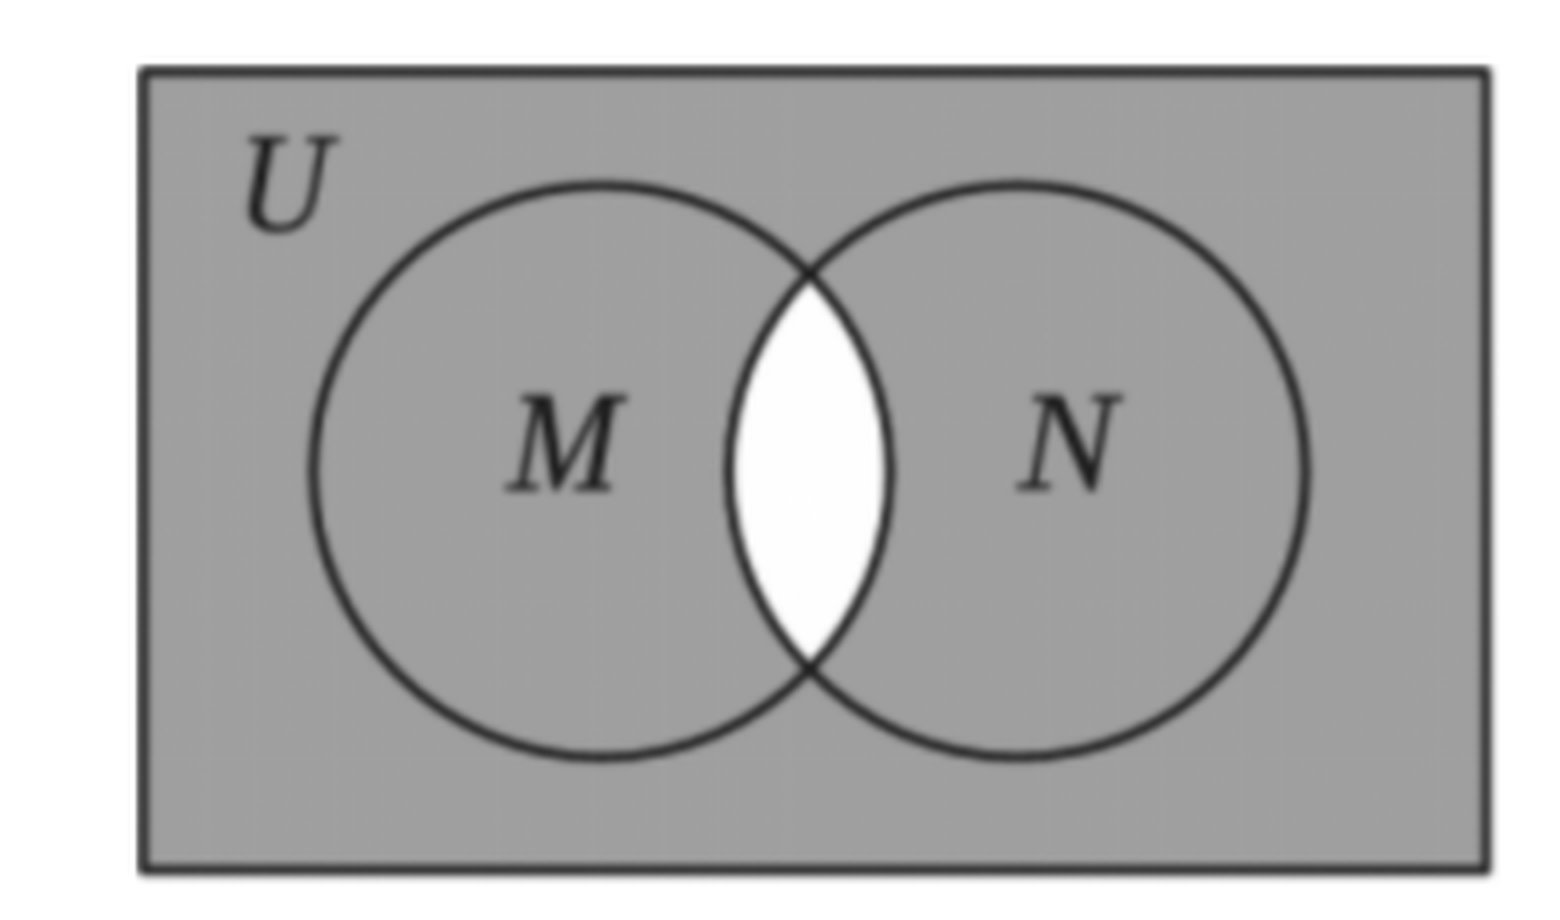
\includegraphics[width=0.40\textwidth]{figures/gao145_q14.png}
\end{center}

\ifanswer
\solbegin
\step{由韦恩图得图中白色区域为集合 $M\cap N$，所以阴影部分表示的集合为 $\overline{M\cap N}$.}
\step{故选 $D$.}
\solend
\fi

% === Q15 ===
\item 已知 $x>-2$，则 $x+\dfrac{1}{x+2}$ 的最小值为\mbox{（\quad）}

\keepwithprev
A. 3\qquad B. 2\qquad C. 1\qquad D. 0

\ifanswer
\solbegin
\step{$x>-2$，则 $x+2>0$，}
\step{所以 $x+\dfrac{1}{x+2}=(x+2)+\dfrac{1}{x+2}-2\geqslant2\sqrt{(x+2)\cdot\dfrac{1}{x+2}}-2=0$，}
\step{当且仅当 $x+2=\dfrac{1}{x+2}$，即 $x=-1$ 时取等号，所以 $x+\dfrac{1}{x+2}$ 的最小值为 $0$.}
\step{故选 $D$.}
\solend
\fi

% 第 16 题：题干在 05 页、解析续至 06 页；两幅数轴标根波浪曲线是【解析】内配图，
% 仅答案版出，放在答案版条件块内 \solbegin 的 \step 之间（照 高一73 第 16 题成例）
\item 关于 $x$ 的不等式 $\dfrac{(x-a)(x-2)^2}{(x-1)(x-5)}\leqslant0$ 的解集中恰有 3 个正整数，则实数 $a$ 的取值范围是\mbox{（\quad）}

\keepwithprev
A. $(-\infty,3]\cup[7,8)$\qquad B. $(-\infty,3)\cup[7,8)$\qquad C. $(-\infty,3]\cup(7,8]$\qquad D. $(-\infty,3)\cup(7,8]$

\ifanswer
\solbegin
\step{由题意，不等式 $\dfrac{(x-a)(x-2)^2}{(x-1)(x-5)}\leqslant0$，}
\step{可化为 $\begin{cases}(x-1)(x-2)^2(x-5)(x-a)\leqslant0\\x\ne1\text{且}x\ne5\end{cases}$，由数轴标根法，}
\step{当 $a=3$ 时，}
\begin{center}
% a=3 数轴标根图取 06 页，去粉色水印、去色、4× LANCZOS 放大；仅答案版出
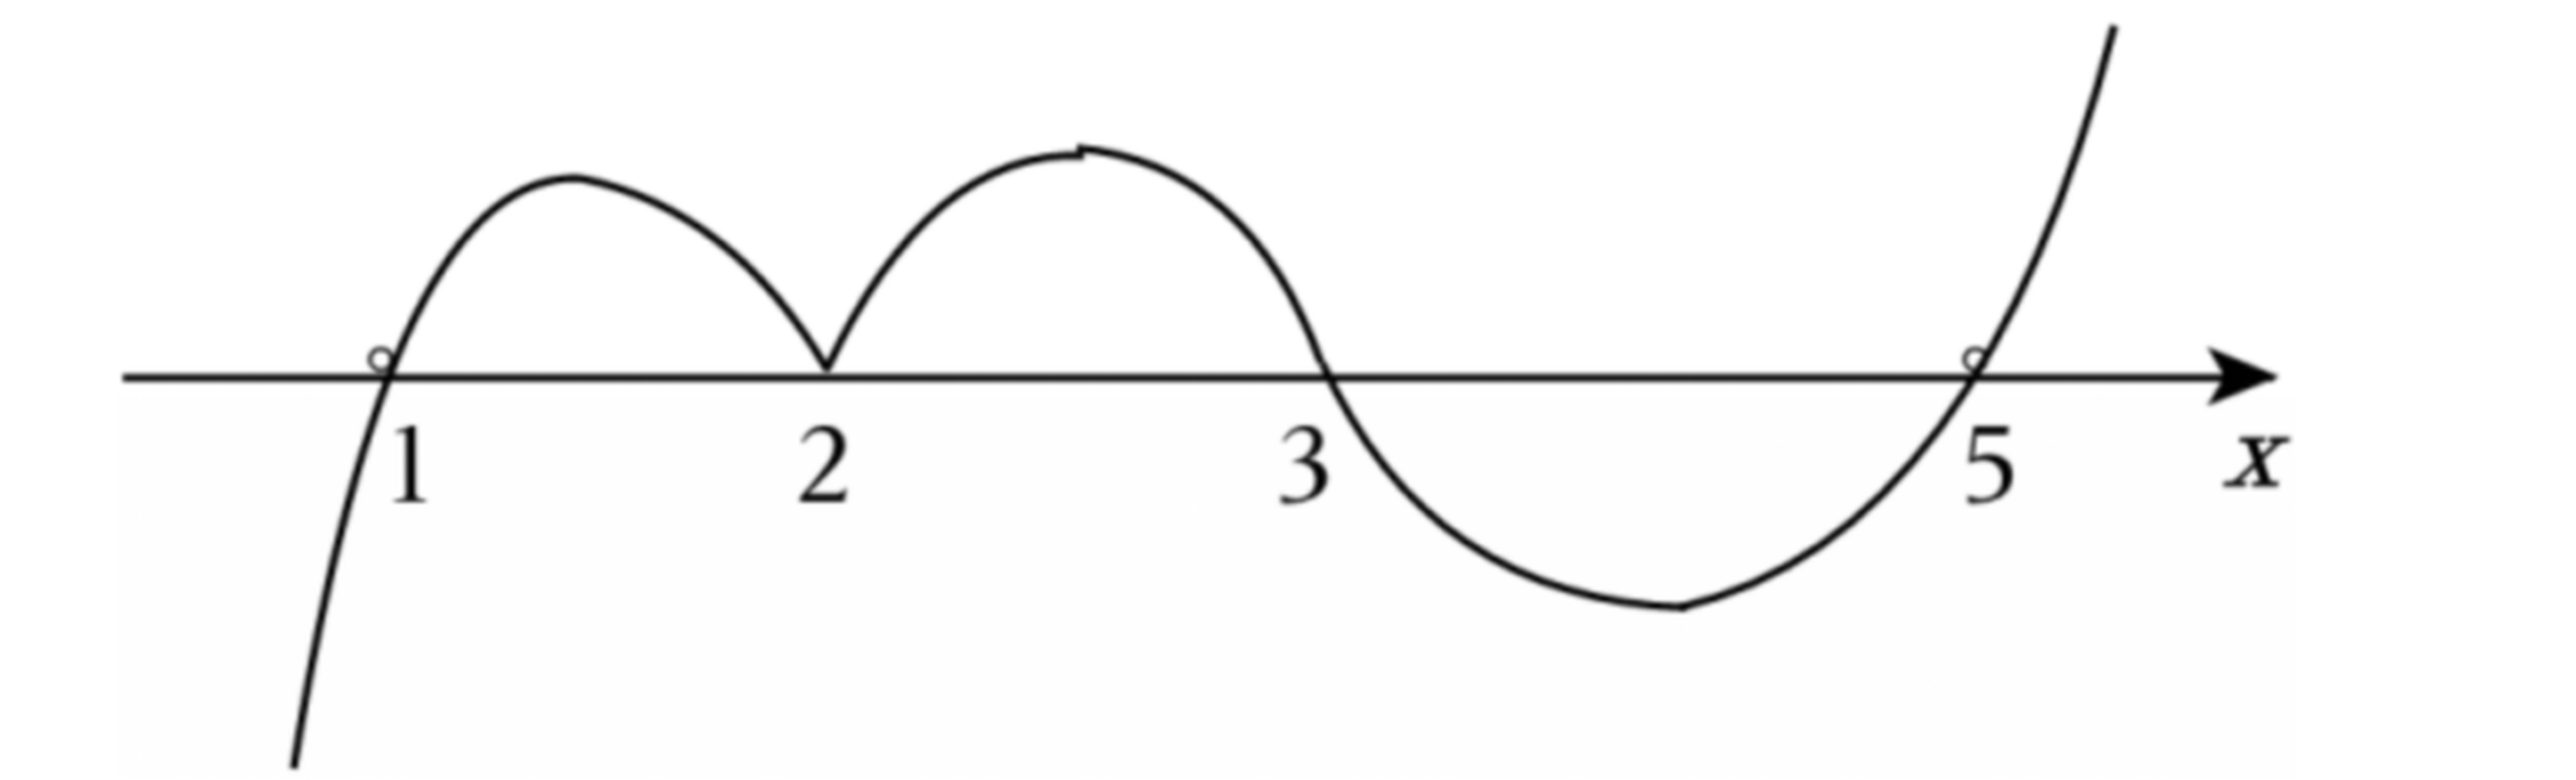
\includegraphics[width=0.62\textwidth]{figures/gao145_q16_a3.png}
\end{center}
\step{得不等式的解集为 $\{x\mid x<1\text{ 或 }x=2\text{ 或 }3\leqslant x<5\}$，}
\step{对应的正整数解为 $2$，$3$，$4$，满足题意，故排除 $B$、$D$；}
\step{当 $a=7$ 时，}
\begin{center}
% a=7 数轴标根图取 06 页，去粉色水印、去色、4× LANCZOS 放大；仅答案版出
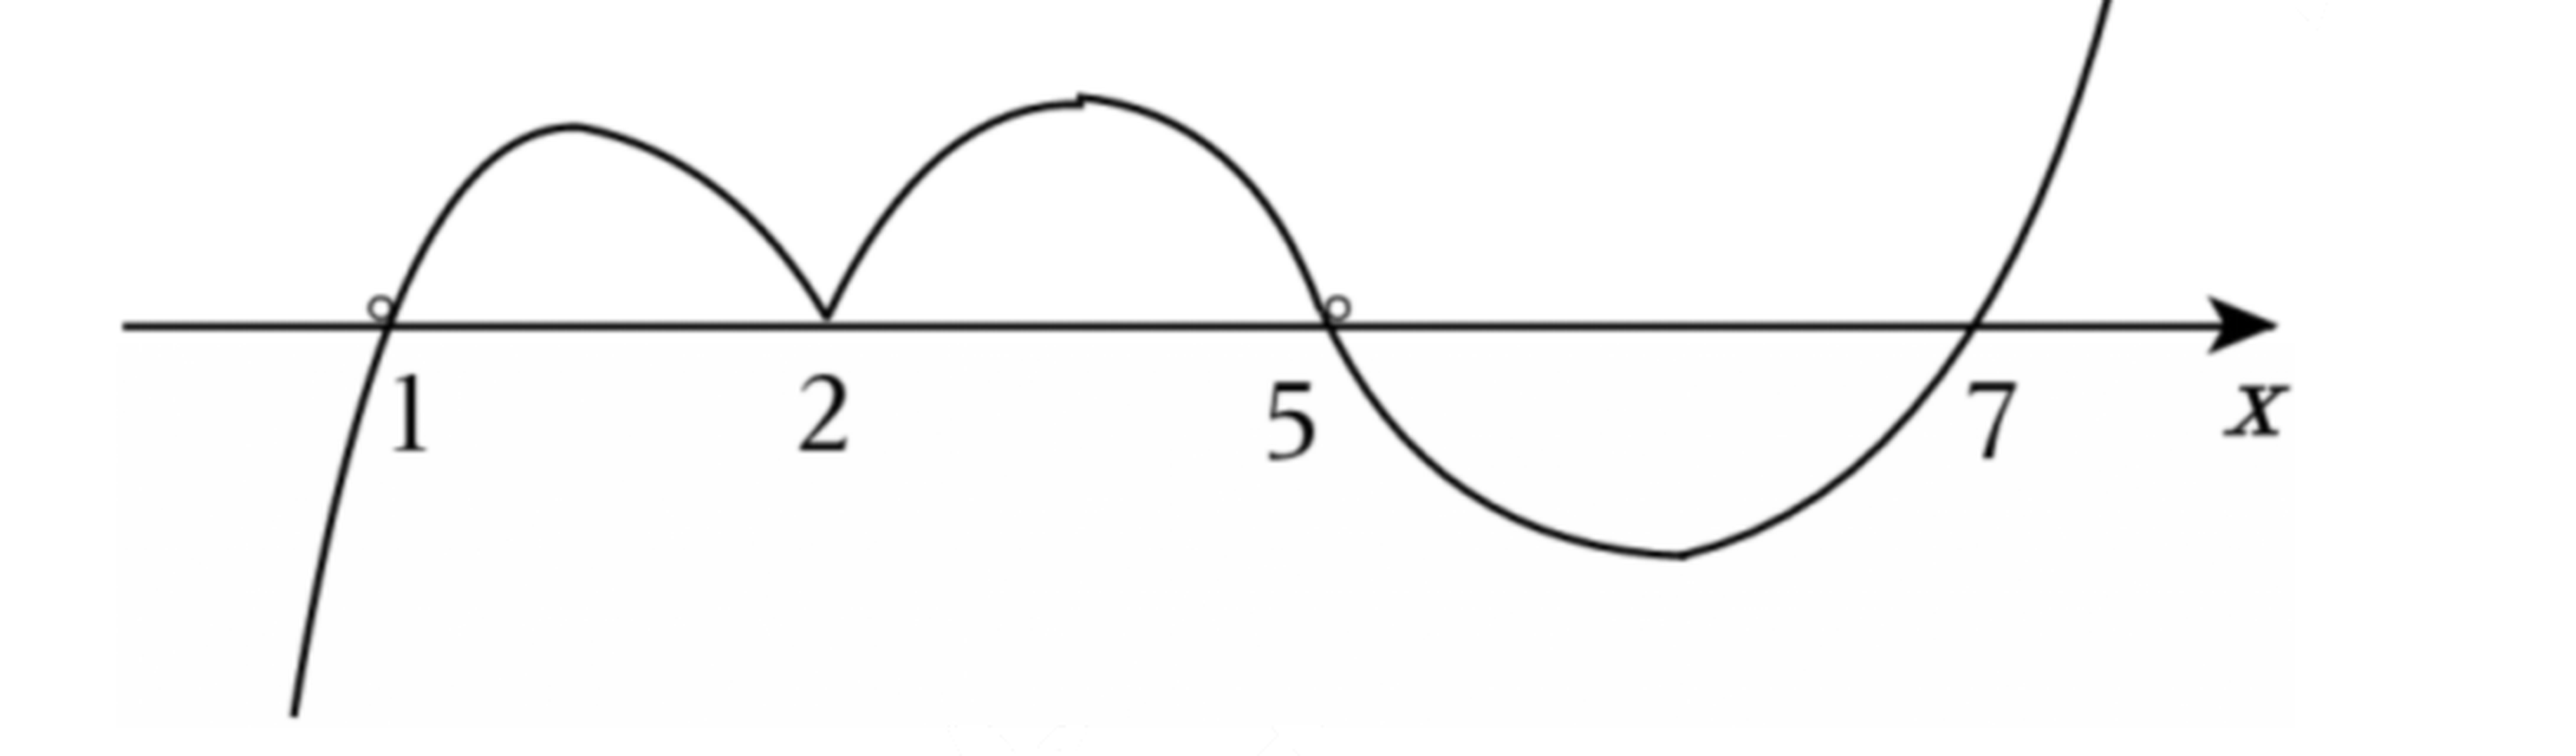
\includegraphics[width=0.62\textwidth]{figures/gao145_q16_a7.png}
\end{center}
\step{得不等式的解集为 $\{x\mid x<1\text{ 或 }x=2\text{ 或 }5<x\leqslant7\}$，}
\step{对应的正整数解为 $2$，$6$，$7$，满足题意，故 $A$ 正确，$C$ 错误.}
\step{故选 $A$.}
\solend
\fi

\end{enumerate}

\bigsec{三、解答题}

\begin{enumerate}
\setcounter{enumi}{16}

% 第 17 题：题干在 06 页、解析续至 07 页，按印刷行断，共 7 行；
% "lg(10÷5)" 的除号照录 \div
\item (1) 已知 $a+a^{-1}=6$，求 $a^2+a^{-2}$ 及 $a^{\frac12}-a^{-\frac12}$ 的值；

(2) 已知 $\lg5=a$，$\lg6=b$，用 $a$、$b$ 分别表示 $\lg2$、$\lg3$、$\lg300$ 和 $\log_{12}15$.

\ifanswer
\solbegin
\step{(1) 因为 $a+a^{-1}=6$，}
\step{所以 $a^2+a^{-2}=(a+a^{-1})^2-2\cdot a\cdot a^{-1}=6^2-2=34$，}
\step{因为 $\left(a^{\frac12}-a^{-\frac12}\right)^2=a-2+a^{-1}=6-2=4$，所以 $a^{\frac12}-a^{-\frac12}=\pm2$；}
\step{(2) $\lg2=\lg(10\div5)=\lg10-\lg5=1-a$，}
\step{$\lg3=\lg(6\div2)=\lg6-\lg2=b-(1-a)=a+b-1$，}
\step{$\lg300=\lg(3\times10^2)=\lg3+\lg10^2=a+b-1+2=a+b+1$，}
\step{所以 $\log_{12}15=\dfrac{\lg15}{\lg12}=\dfrac{\lg3+\lg5}{\lg3+\lg2^2}=\dfrac{a+b-1+a}{a+b-1+2(1-a)}=\dfrac{2a+b-1}{b-a+1}$.}
\solend
\fi

% 第 18 题：题干在 07 页、解析续至 08 页（2 问、分类讨论很长），按印刷行断共 25 行；
% 本卷 Q18 用"图像"（Q13/Q14 用"图象"），逐处照录不统一
\item 已知 $f(x)=(m^2-3m+1)x^{m^2-4m-1}$，$y=f(x)$ 为幂函数且在 $(0,+\infty)$ 上是严格减函数.

(1) 求实数 $m$ 的值以及相应的函数表达式；

(2) 若 $y=f(x)$ 的图像关于 $y$ 轴对称，解关于 $x$ 的不等式 $(x+2)^{1-m}<(3x-1)^{1-m}$.

\ifanswer
\solbegin
\step{(1) 由幂函数的定义得 $m^2-3m+1=1$，}
\step{整理得 $m^2-3m=0$，解得 $m=0$ 或 $m=3$，}
\step{由于 $y=f(x)$ 在 $(0,+\infty)$ 上为严格减函数，}
\step{因此幂函数的指数需满足 $m^2-4m-1<0$，}
\step{当 $m=3$ 时，指数为 $3^2-4\times3-1=-4<0$，满足严格递减条件，}
\step{此时函数表达式为 $f(x)=x^{-4}$，}
\step{当 $m=0$ 时，指数为 $0^2-4\times0-1=-1<0$，满足严格递减条件，}
\step{此时函数表达式为 $f(x)=x^{-1}$，}
\step{所以满足条件的实数 $m$ 为 $0$ 或 $3$，}
\step{对应的函数表达式分别为 $f(x)=x^{-1}$、$f(x)=x^{-4}$；}
\step{(2) 函数图像关于 $y$ 轴对称即函数为偶函数，}
\step{对于 $f(x)=x^{-1}=\dfrac1x$，定义域为 $(-\infty,0)\cup(0,+\infty)$，}
\step{满足 $f(-x)=-f(x)$，为奇函数，图像关于原点对称，}
\step{不满足关于 $y$ 轴对称的条件；}
\step{对于 $f(x)=x^{-4}=\dfrac{1}{x^4}$，定义域为 $(-\infty,0)\cup(0,+\infty)$，}
\step{满足 $f(-x)=f(x)$，为偶函数，图像关于 $y$ 轴对称，}
\step{因此符合条件的 $m$ 值为 $3$，}
\step{将 $m=3$ 代入关于 $x$ 的不等式 $(x+2)^{1-m}<(3x-1)^{1-m}$，}
\step{得 $(x+2)^{1-3}<(3x-1)^{1-3}$，即 $(x+2)^{-2}<(3x-1)^{-2}$，}
\step{因为负指数幂的底数不能为 $0$，所以 $x+2\ne0$ 且 $3x-1\ne0$，}
\step{即 $x\ne-2$ 且 $x\ne\dfrac13$，}
\step{不等式可变形为 $\dfrac{1}{(x+2)^2}<\dfrac{1}{(3x-1)^2}$，}
\step{整理得 $(3x-1)^2<(x+2)^2$，即 $8x^2-10x-3<0$，}
\step{解得 $-\dfrac14<x<\dfrac32$，又 $x\ne-2$ 且 $x\ne\dfrac13$，}
\step{所以不等式的解集为 $\left(-\dfrac14,\dfrac13\right)\cup\left(\dfrac13,\dfrac32\right)$.}
\solend
\fi

% 第 19 题：题干在 08 页、解析续至 09 页，按印刷行断，共 14 行；
% 判别式 cases 块内"△=4a²−16a<0"原卷印扁等边三角 \triangle
%（放大 09 页 zz09_delta.png 与 Q12 高 \Delta 并排确认），逐处照录不统一
\item 已知 $f(x)=ax^2+2ax+4$，$a\in\R$.

(1) 若关于 $x$ 的不等式 $f(x)>0$ 在实数集 $\R$ 上恒成立，求实数 $a$ 的取值范围；

(2) 当 $a<0$ 时，解关于 $x$ 的不等式 $f(x)>(a+1)x+5$.

\ifanswer
\solbegin
\step{(1) 由题意得，关于 $x$ 的不等式 $f(x)>0$ 在实数集 $\R$ 上恒成立，}
\step{即 $ax^2+2ax+4>0$ 在实数集 $\R$ 上恒成立，}
\step{当 $a=0$ 时，不等式为 $4>0$ 恒成立，符合题意；}
\step{当 $a\ne0$ 时，则 $\begin{cases}a>0\\\triangle=4a^2-16a<0\end{cases}$，解得 $0<a<4$.}% 判别式原卷印扁等边三角 $\triangle$，照录
\step{综上所述，实数 $a$ 的取值范围为 $[0,4)$.}
\step{(2) $f(x)=ax^2+2ax+4$，}
\step{当 $a<0$ 时，不等式 $f(x)>(a+1)x+5$ 即为 $ax^2+(a-1)x-1>0$，}
\step{即 $(ax-1)(x+1)>0$，即 $\left(x-\dfrac1a\right)(x+1)<0$，}
\step{当 $a<-1$，即 $\dfrac1a>-1$ 时，解得 $-1<x<\dfrac1a$；}
\step{当 $a=-1$，即 $\dfrac1a=-1$ 时，解得 $x\in\varnothing$；}
\step{当 $-1<a<0$，即 $\dfrac1a<-1$ 时，解得 $\dfrac1a<x<-1$.}
\step{综上所述，当 $a<-1$ 时，不等式的解集为 $\left\{x\mid -1<x<\dfrac1a\right\}$；}
\step{当 $a=-1$ 时，不等式的解集为 $\varnothing$；}
\step{当 $-1<a<0$ 时，不等式的解集为 $\left\{x\mid \dfrac1a<x<-1\right\}$.}
\solend
\fi

% 第 20 题：菜园靠墙图为题目配图（三版都出），题干写"如图"；
% 题干在 09 页（含图）、解析续至 10 页，按印刷行断，共 13 行
\needvspace{8cm}
\item 如图，某人计划用篱笆围成一个一边靠墙（墙足够长）的矩形菜园. 设菜园的长为 $x$ 米，宽为 $y$ 米.

\begin{center}
% 矩形菜园靠墙图取 09 页右下，去粉色水印、去色、4× LANCZOS 放大
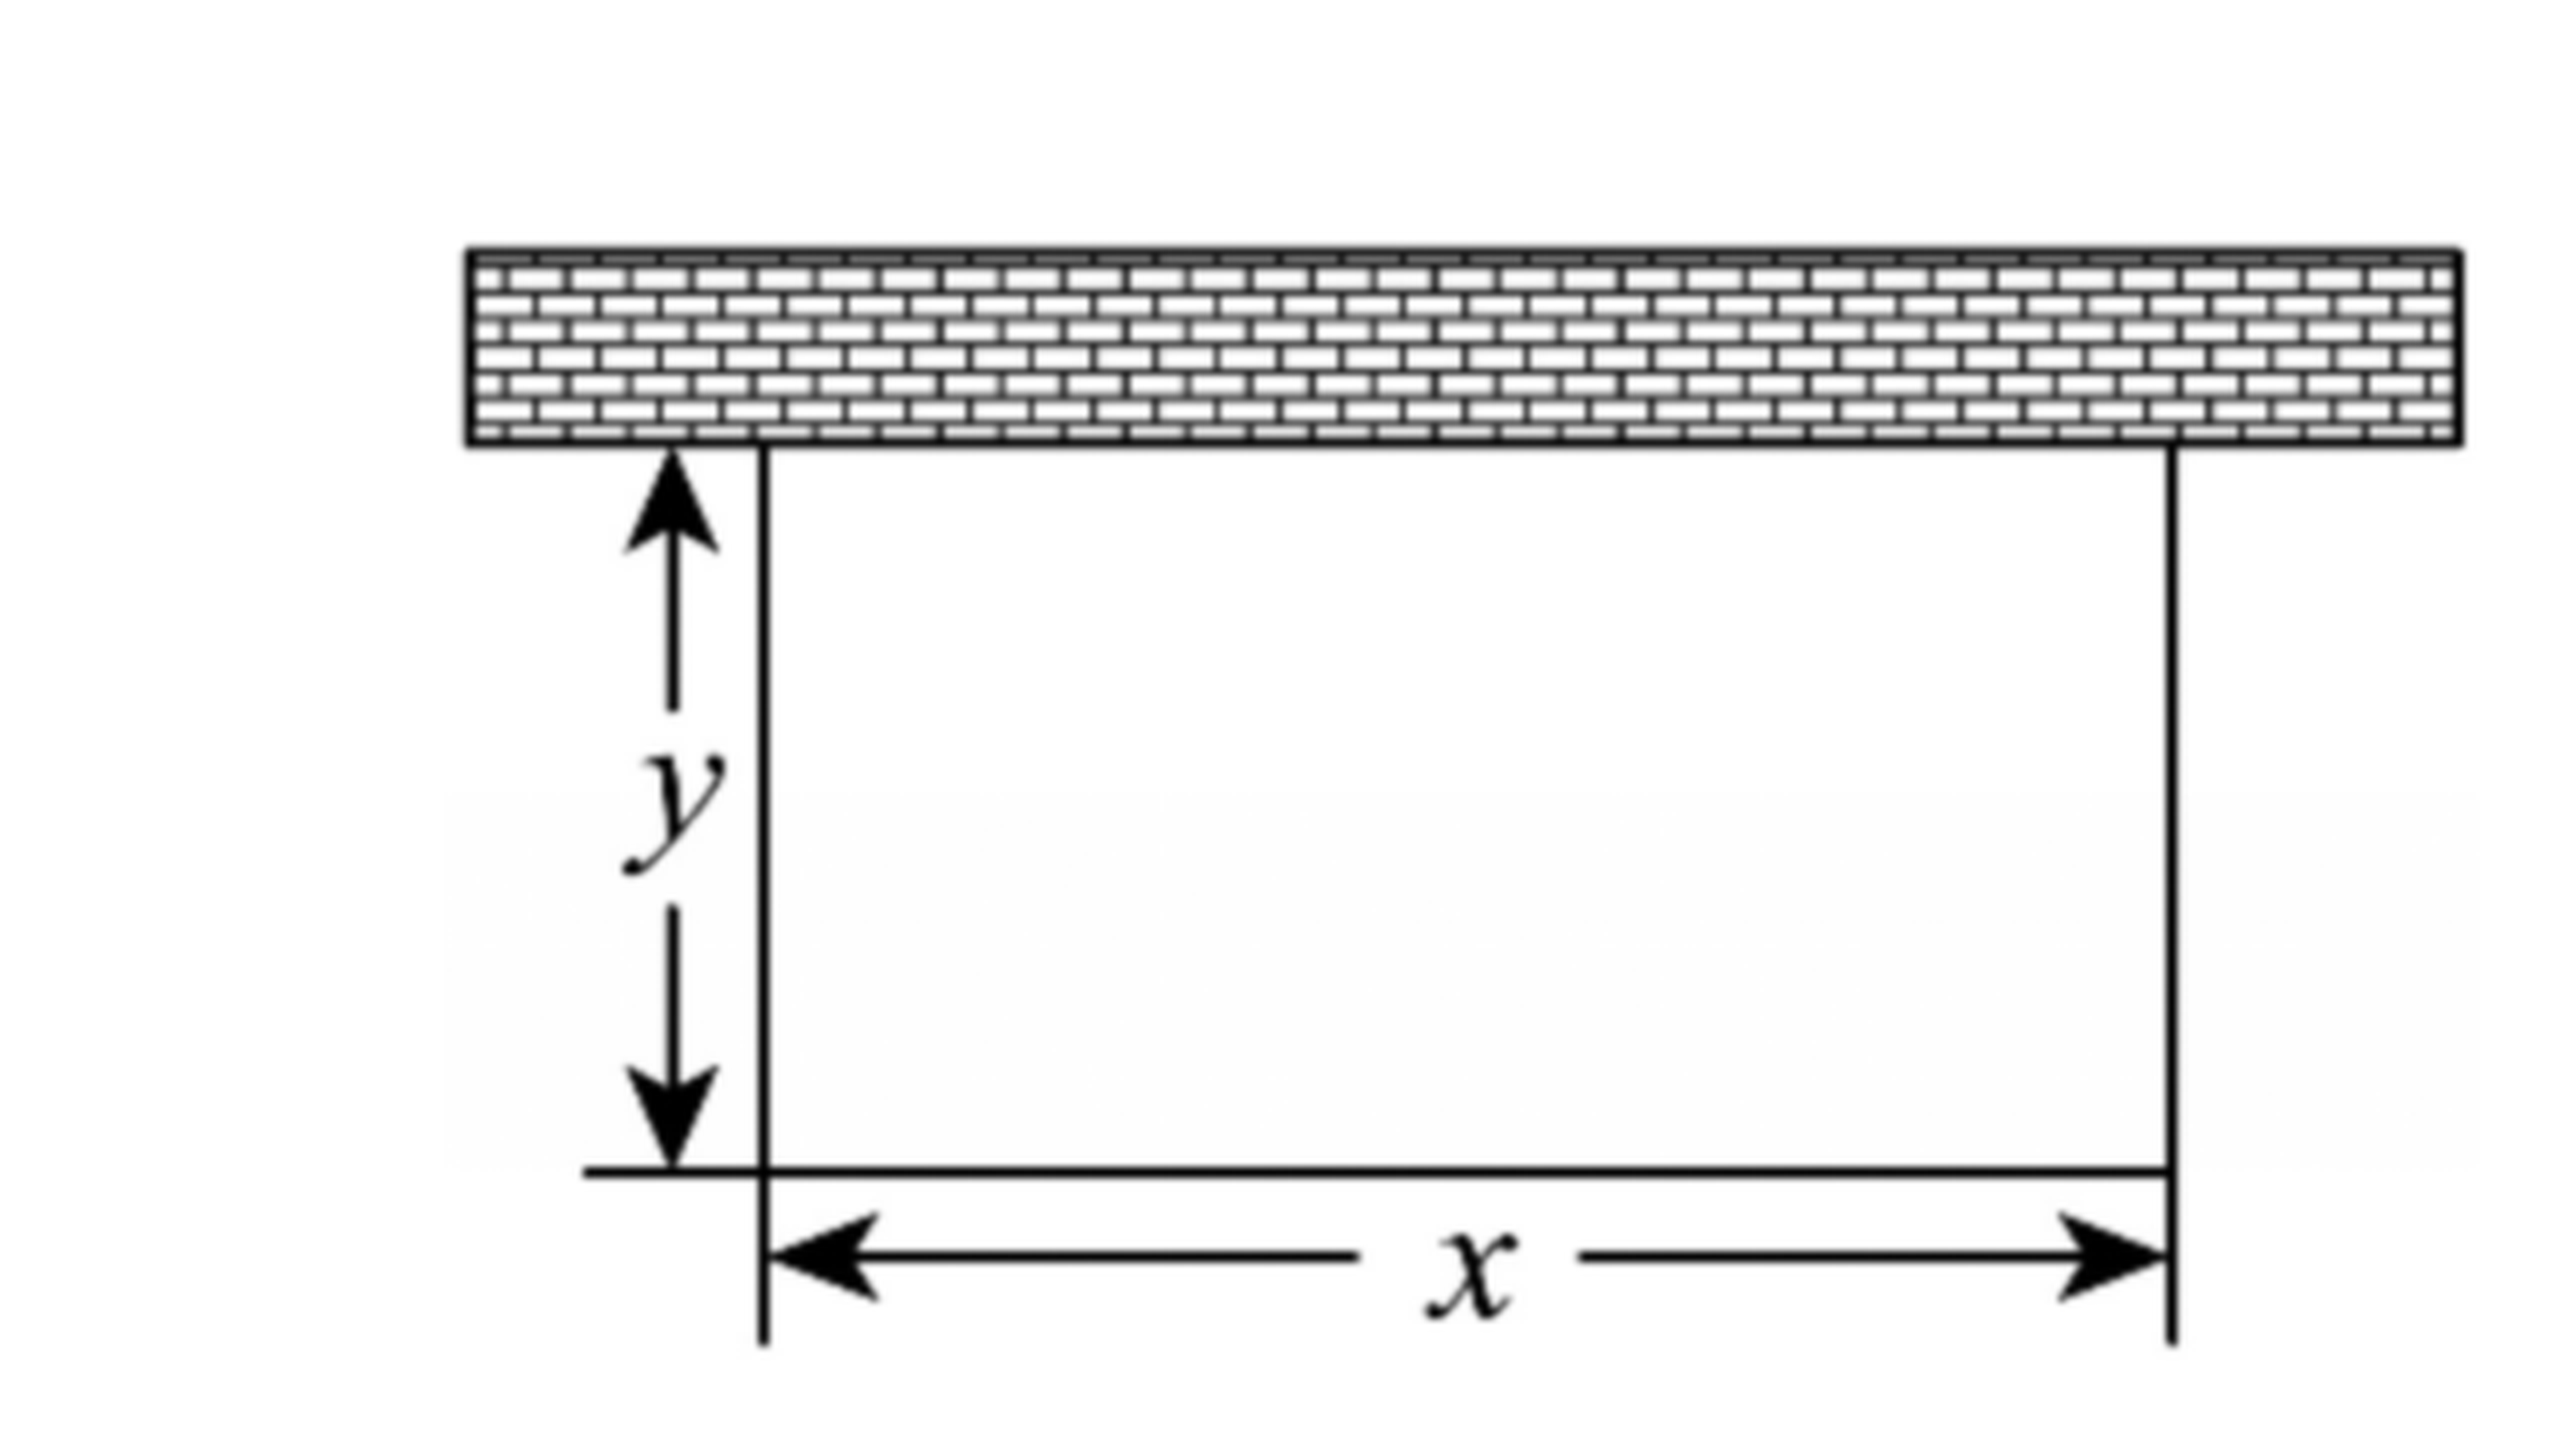
\includegraphics[width=0.55\textwidth]{figures/gao145_q20.png}
\end{center}

(1) 若菜园面积为 72 平方米，则 $x$、$y$ 为何值时，所用篱笆总长最小？

(2) 若 $x$、$y$ 满足 $x+y-xy+63=0$，则菜园面积最小为多少平方米？

\ifanswer
\solbegin
\step{(1) 由题意得，菜园的面积 $S=xy=72$，且 $x>0$，$y>0$，}
\step{所用篱笆总长 $L=x+2y$，}
\step{由基本不等式得 $x+2y\geqslant2\sqrt{x\cdot2y}=2\sqrt{2xy}=2\sqrt{2\times72}=24$，}
\step{当且仅当 $x=2y$ 时取等号，}
\step{联立 $\begin{cases}xy=72\\x=2y\end{cases}$，解得 $\begin{cases}x=12\\y=6\end{cases}$，}
\step{所以当 $x=12$，$y=6$ 时，所用篱笆总长最小；}
\step{(2) 由题意得 $x>0$，$y>0$，且满足 $x+y-xy+63=0$，即 $x+y=xy-63$，}
\step{由基本不等式得 $x+y\geqslant2\sqrt{xy}$，当且仅当 $x=y$ 时取等号，}
\step{所以 $xy-63\geqslant2\sqrt{xy}$. 令 $t=\sqrt{xy}(t>0)$，则 $xy=t^2$，}
\step{上述不等式可化为 $t^2-2t-63\geqslant0$，即 $(t-9)(t+7)\geqslant0$，}
\step{因为 $t>0$，所以 $t+7>0$，故 $t-9\geqslant0$，解得 $t\geqslant9$，所以 $\sqrt{xy}\geqslant9$，}
\step{即 $xy\geqslant81$，当且仅当 $x=y=9$ 时取等号，此时满足 $9+9-81+63=0$，}
\step{所以菜园面积最小为 81 平方米.}
\solend
\fi

% 第 21 题：题干在 10 页、解析续至 11 页（3 问、分类讨论很长），按印刷行断共 22 行；
% 末行"故第 2026 个元素是 2700 之后第一个属于 A 的数，即 2701." 为全卷收尾，
% 无 Q22/Q23、无附加题节；数集 Z/N* 按全稿惯例改 \Z/\N^*
\item 已知集合 $A=\{x\mid x=m^2-n^2$，$m$、$n\in\Z\}$.

(1) 求证：任何奇数 $2k+1(k\in\Z)$ 都是集合 $A$ 中的元素；

(2) 判断偶数 $4k-2(k\in\Z)$ 是否为集合 $A$ 的元素？请说明理由；

(3) 若将集合 $A$ 中的正整数由小到大排列，求出集合 $A$ 中第 2026 个正整数.

\ifanswer
\solbegin
\step{(1) 因为 $x=(k+1)^2-k^2=2k+1(k\in\Z)$，}
\step{所以任何奇数 $2k+1(k\in\Z)$ 都属于集合 $A$；}
\step{(2) 偶数 $4k-2(k\in\Z)$ 不是集合 $A$ 的元素，理由如下：}
\step{由题意得 $x=m^2-n^2=(m-n)(m+n)$，}
\step{当 $m$、$n$ 均为奇数时，设 $m=2k_1+1$，$n=2k_2+1(k_1$、$k_2\in\Z)$，}
\step{则 $m^2-n^2=(2k_1+1)^2-(2k_2+1)^2=(2k_1-2k_2)(2k_1+2k_2+2)$}
\step{$=4(k_1-k_2)(k_1+k_2+1)$，}
\step{因为 $k_1$、$k_2\in\Z$，所以 $k_1-k_2\in\Z$，$k_1+k_2+1\in\Z$，}
\step{从而 $m^2-n^2$ 为 $4$ 的倍数；}
\step{当 $m$、$n$ 均为偶数时，设 $m=2k_1$，$n=2k_2(k_1$、$k_2\in\Z)$，}
\step{$m^2-n^2=4k_1^2-4k_2^2=4(k_1^2-k_2^2)$ 为 $4$ 的倍数；}
\step{当 $m$、$n$ 为一个偶数一个奇数时，不妨设 $m$ 为偶数，$n$ 为奇数，}
\step{设 $m=2k_1$，$n=2k_2+1(k_1$、$k_2\in\Z)$，}
\step{则 $m^2-n^2=4k_1^2-(2k_2+1)^2=4(k_1^2-k_2^2-k_2)-1$ 为奇数.}
\step{无论哪种情况均不满足 $4k-2(k\in\Z)$，}
\step{故偶数 $4k-2(k\in\Z)$ 不是集合 $A$ 的元素；}
\step{(3) 由前两问得，$4$ 的倍数和奇数属于集合 $A$ 中的元素，}
\step{令集合 $A$ 中的正整数元素为 $4k-3$、$4k-1$、$4k(k\in\N^*)$，}
\step{对任意的 $k\in\N^*$，连续的 $4$ 个整数 $4k-3$、$4k-2$、$4k-1$、$4k$ 中}
\step{有三个数 $4k-3$、$4k-1$、$4k$ 都在集合 $A$ 中，}
\step{因为 $2026=3\times675+1$，所以集合 $A$ 中第 $2025$ 个元素为 $4\times675=2700$，}
\step{故第 2026 个元素是 2700 之后第一个属于 $A$ 的数，即 2701.}
\solend
\fi

\end{enumerate}

\end{document}
"
%
% ① 原始材料：微信公众号"魔都数学加油站"文章，连载"27学年高一145"，原文标题
% "27学年高一145——2026-2027年上海市市二中学高一上期中"；
% 原文链接：https://mp.weixin.qq.com/s/6V-i9KE0GWodC-wmd5z8nQ 。
% 正文为 11 张 PNG 页（01/02/03/08/10/11 为 4762×6735，04/05/06/07/09 为 2560×3620，
% 同一篇各页分辨率不同，逐页按各自分辨率裁图核对，别按预览比例换算裁框）。
% 题目下印【答案】或【解析】，为混合体例讲评版：Q3 只印【答案】、无【解析】，其余
% 18 题印【解析】。题目、解析均据原图转录；卷面粉红色水印"魔都数学加油站"及
% 公众号页脚未录入。
% 全卷插图情况（逐页通读 11 页确认，题干写"如图"处均配有图）：
%   · Q14 韦恩图（05 页右侧，全集 U 矩形＋两圆 M/N＋白色交集、灰色阴影＋U/M/N 标注）：
%     题目配图（选择题选项旁），三版都出，裁自 05 页去水印去色 4× 放大存
%     figures/gao145_q14.png；
%   · Q16 两幅数轴标根波浪曲线（06 页，a=3 与 a=7 各一幅，标根法画
%     (x-1)(x-2)^2(x-5)(x-a)≤0 的符号曲线）：【解析】内的配图，仅答案版出，
%     裁 figures/gao145_q16_a3.png / figures/gao145_q16_a7.png（或合并一张），
%     放在答案版条件块内 \solbegin 的 \step 之间（照 高一73 第 16 题成例）；
%   · Q20 矩形菜园靠墙图（09 页右下，灰色砖墙＋矩形菜园＋x/y 标注＋箭头）：
%     题目配图，三版都出，裁自 09 页去水印去色 4× 放大存 figures/gao145_q20.png；
%   其余各页逐页确认无其它题目配图、无表格、亦无"题干写如图而源码漏图"一处。
%
% 卷首标题：原卷印作"2026-2027 年市二中学高一上期中"，年份区间按全稿惯例排 en dash；
% 原卷卷面未印副标题，本稿按同期中卷（高一140／141／143／144）知识模块口径补出
% "集合与常用逻辑用语、不等式、函数"。
%
% 题号体例：本卷共 19 题——一、填空题 3—12（10 题）、二、选择题 13—16（4 题）、
% 三、解答题 17—21（5 题）。三节分别 \setcounter{enumi}{2}／{12}／{16}。
% 原卷从第 3 题起、无第 1、2 题，本稿保留原题号；全卷无附加题节。
%
% ② 与原卷的排版差异：
%   ① 原文从第 3 题起，本稿保留原题号；共 19 题三节；
%   ② 混合体例：原卷 Q3 只印【答案】、无【解析】（"第一步应假设___。
%      【答案】x≤2 或 y≤2"），按 高一140 第 5 题成例提 \ans{}、不补造解析；
%      其余 18 题印【解析】，用 \solbegin…\solend，选择题答案在解析末句"故选 X"
%      （Q13 选 B、Q14 选 D、Q15 选 D、Q16 选 A，逐个放大原图核实）、
%      题干括号 \mbox{（\quad）} 留空、不另提 \ans{}；填空／解答答案落在解析里；
%      答案版【答案】/【解析】标记数 = 19（1 个 \ans ＋ 18 个 \solbegin）= 全卷题数；
%   ③ 原卷卷面未印副标题，本稿按知识模块口径补出；
%   ④ 原卷填空横线按全稿惯例排 \blankline[4.4em]；选择题括号排 \mbox{（\quad）}、
%      选项段前按惯例加 \keepwithprev；解答题不留作答区、不加 \anspace
%      （原卷为讲评版，与 129／131／132／133／136／140／141／143／144 同）；
%   ⑤ 数集：Q9"a、b∈R"、Q12"a∈R"、Q21"m、n∈Z""k∈Z""k∈N*"等原卷印
%      斜体或黑板粗体 R/Z/N，按全稿惯例统一改 \R／\Z／\N^*；绝对值排 \lvert…\rvert，
%      集合描述竖线排 \mid；不等号按全稿惯例排 \leqslant／\geqslant；
%      补集照原卷上划线排 \overline{M}／\overline{N}（Q14 选项 B/C/D 逐处核）；
%      空集记号 \varnothing；\subset（单线⊂）与 \subseteq（带下划线⊆）逐处照录不统一；
%   ⑥ 子题标号 (1)(2)(3) 原卷印半角括号照录；圈数字进数学式用 \text{①}（否则 FONTCHK 挂）；
%      \left…\right 不得拆到不同 $…$ 组；cases 块整体算一个印刷行；
%   ⑦ 题干／解析中的中文弯引号按原卷照录（Q3"若 x+y>4，则 x>2 且 y>2"、
%      Q11"a₁/a₂=b₁/b₂""M=N"、选填"充分非必要""必要非充分""充要""既非充分也非必要"
%      等，含引号内空格），注释内一律 ASCII 引号；数学式内 CJK 用 \text{}；
%   ⑧ 半角逗号在数学组之间是全稿惯例、非笔误（如 Q5"x₁+x₂=6，x₁x₂=√3"、
%      Q7"a>1，b>1"、指数／对数式内逗号），逐处照录别改全角；行末西文句点照录为
%      ASCII `.`；行中全角逗号／顿号照录；
%   ⑨ "图像／图象"逐处照录不统一（Q18"图像关于 y 轴对称"等，核全卷）；
%   ⑩ 判别式 Δ/△ 混用是照录项：Q12 解析"Δ=a²−4a²(2a−3)>0"、
%      Q19 解析"Δ=4a²−16a<0"等，放大原图判断是高 \Delta（等腰偏高、高>宽）
%      还是扁 \triangle，逐处照录不得统一（参照 高一142／144 头注④口径）；
%   ⑪ 一条 \step = 原卷解析的一个印刷行，cases 块整体算一个印刷行；别把原卷折行
%      并起来、别把一行拆多条。Q6 分段讨论、Q12 三个 cases 条件组、Q16 数轴标根、
%      Q18／Q19 分类讨论、Q21 三问均按印刷行逐条断，不丢行；
%   ⑫ Q14 韦恩图为"题干＋选项＋图"整块，加 \needvspace 守卫推走（守卫放 \item 之前，
%      见 高一140 Q14、高一144 Q17 成例与切页审计 B 类坑）；Q20 菜园图同理；
%      三版切页审计均"合计异常：无"；
%   ⑬ 跨页续印按题合并：Q3/4/5/6 在 01 页（Q6 解析续 02 页顶）；Q7/8/9/10 在 02 页
%      （Q10 解析续 03 页）；Q11/12 在 03 页（Q12 解析续 04 页，很长）；
%      Q13 在 04 页末、解析在 05 页顶；Q14/15/16 在 05 页（Q16 解析续 06 页含两幅数轴图）；
%      Q17 在 06 页、解析续 07 页；Q18 在 07 页、解析续 08 页；Q19 在 08 页、解析续 09 页；
%      Q20 在 09 页（含菜园图）、解析续 10 页；Q21 在 10 页、解析续 11 页
%      （末页收尾"故第 2026 个元素是 2700 之后第一个属于 A 的数，即 2701."、
%      无 Q22/Q23、无附加题节）。本稿按题连排，不丢行、不并折行；
%   ⑭ 原卷解析内若有红色"法一／法二"之类小标题，按全稿惯例排 \stepm{标签}{…}
%      （黑体着色、不引入红色、不改 common.sty），头注注明；水印"魔都数学加油站"
%      红色不录入。
%
% ③ 行数复核：一条 \step／\stepm = 原卷解析的一个印刷行，cases 块作一个印刷行计。
%   逐题数（主会话逐页核对定稿）：Q3：0（只印【答案】、提 \ans{}，不计入 \step 账）；
%   Q4：3；Q5：2；Q6：10；Q7：3；Q8：3；Q9：2；Q10：7；Q11：4；Q12：12；
%   Q13：2；Q14：2；Q15：4；Q16：9；Q17：7；Q18：25；Q19：14；Q20：13；Q21：22。
%   合计 144 条 \step（本卷无 \stepm：解析内无红色"法一／法二"类小标题），
%   与原卷逐题印刷行相等。全卷 18 题设 \solbegin…\solend ＋ Q3 一处 \ans{}，
%   答案版【答案】/【解析】标记数 = 19 = 全卷题数。
%
% ④ 判别式／子集符号结论（逐处放大原图照录、不得统一，主会话像素级复核）：
%   判别式全卷 2 处、两形混用逐处照录不统一（参照 高一142／144 头注④口径）：
%     · Q12 解析 cases 块"Δ=a²−4a²(2a−3)>0" 原卷印等腰偏高粗三角（高>宽），
%       照录 \Delta（放大 04 页 /tmp/gao145s2/main_q12_delta.png 确认）；
%     · Q19 解析 cases 块"△=4a²−16a<0" 原卷印扁等边空心三角（宽≈高、细线），
%       照录 \triangle（放大 09 页 /tmp/gao145s2/main_q19_delta.png 确认）。
%   子集／补集：Q14 选项 A `M\cup N`、B `M\cap\overline{N}`（上划线只在 N 上）、
%   C `\overline{M\cup N}`（罩整个 M∪N）、D `\overline{M\cap N}`（罩整个 M∩N，
%   非 \overline{M}\cap N；放大 05 页 /tmp/gao145s2/main_q14_opts.png 确认），
%   阴影为灰色区域＝全集减白色交集，答案 D，照录 \overline{M\cap N}；
%   全集卷无 \subset／\subseteq 混用（本卷集合题用 \cup／\cap／\overline{}）；
%   空集 \varnothing（Q19 解析 x∈\varnothing）；数集 \R／\Z／\N^* 归一见 ② ⑤。
%
% ⑤ 存疑照录（放大原图确认，照录未改、正文对应处另有 % 注）：
%   1. Q3 题干"若 x+y>4，则 x>2 且 y>2" 后"时"前留一空格、弯引号内空格照录；
%      该卷混合体例（Q3 只印【答案】、提 \ans{}）见 ② ②。
%   2. Q4／Q5 解析中的"1，3，5 和 6"、"x₁+x₂=6,x₁x₂=√3" 等半角／全角逗号
%      逐处照原卷（放大 01 页确认），数学式内半角逗号为全稿惯例、非笔误。
%   3. Q14 选项 D 上划线罩住整个 M∩N（而非仅罩 M），照录 \overline{M\cap N}。
%   4. Q12 判别式高 \Delta 与 Q19 判别式扁 \triangle 两形混用，逐处照录不统一（见 ④）。
%   全卷除此 4 类外未发现其它笔误／自相矛盾处。
%
% ⑥ 跨页续印按题合并说明：见 ② ⑬。
%
\documentclass[a4paper,11pt]{article}
\usepackage{common}

\begin{document}

\examtitlest[3]{2026--2027 年市二中学高一上期中}{集合与常用逻辑用语、不等式、函数}

\bigsec{一、填空题}

\begin{enumerate}
\setcounter{enumi}{2}

% 第 3 题：原卷只印【答案】、无【解析】（放大 01 页确认），按 高一140 第 5 题成例
% 提 \ans{}、不补造解析；题干中文弯引号与"时"前空格照录
\item 用反证法证明命题：“若 $x+y>4$，则 $x>2$ 且 $y>2$” 时，第一步应假设\blankline[4.4em].

\ifanswer
\ans{$x\leqslant2$ 或 $y\leqslant2$}
\fi

% === Q4 ===
\item 设集合 $M$ 满足 $\{1,3,5,6\}\cup M=\{1,2,3,4,5,6\}$，则满足条件的所有 $M$ 的个数为\blankline[4.4em].

\ifanswer
\solbegin
\step{集合 $M$ 满足 $\{1,3,5,6\}\cup M=\{1,2,3,4,5,6\}$，}
\step{则 $M$ 中必含有 $2$ 和 $4$，$1$，$3$，$5$ 和 $6$ 可以选也可不选，}
\step{则满足条件的所有 $M$ 的数目相当于集合 $\{1,3,5,6\}$ 的子集的个数 $2^4=16$.}
\solend
\fi

% === Q5 ===
\item 已知方程 $x^2-6x+\sqrt3=0$ 的两根为 $x_1$ 和 $x_2$，则 $(x_1-x_2)^2=$\blankline[4.4em].

\ifanswer
\solbegin
\step{因为方程 $x^2-6x+\sqrt3=0$ 的两根为 $x_1$ 和 $x_2$，所以 $x_1+x_2=6,x_1x_2=\sqrt3$，}% 数学式内半角逗号为全稿惯例，照录
\step{所以 $(x_1-x_2)^2=(x_1+x_2)^2-4x_1x_2=36-4\sqrt3$.}
\solend
\fi

% 第 6 题：题干在 01 页，解析续至 02 页顶（末 2 行），按印刷行逐条断，共 10 行
\item 不等式 $\lvert x-2026\rvert+\lvert x-2029\rvert>3$ 的解集是\blankline[4.4em].

\ifanswer
\solbegin
\step{当 $x<2026$ 时，$x-2026<0$，$x-2029<0$，}
\step{原不等式可化为 $(2026-x)+(2029-x)>3$，解得 $x<2026$，}
\step{故此时，不等式的解为 $x<2026$；}
\step{当 $2026\leqslant x\leqslant2029$ 时，$x-2026\geqslant0$，$x-2029\leqslant0$，}
\step{原不等式可化为 $(x-2026)+(2029-x)>3$，即 $3>3$，显然不成立，}
\step{故此时，不等式无解；}
\step{当 $x>2029$ 时，$x-2026>0$，$x-2029>0$，}
\step{原不等式可化为 $(x-2026)+(x-2029)>3$，解得 $x>2029$，}
\step{故此时，不等式的解为 $x>2029$.}
\step{综上，原不等式的解集为 $(-\infty,2026)\cup(2029,+\infty)$.}
\solend
\fi

% === Q7 ===
\item 已知 $a>1$，$b>1$，若 $\log_a b+\log_b a=2$，且 $ab=2$，则 $\log_2(a+b)=$\blankline[4.4em].

\ifanswer
\solbegin
\step{由 $\log_a b+\log_b a=2$，$a>1$，$b>1$，得 $\log_a b+\dfrac{1}{\log_a b}=2$，}
\step{即 $(\log_a b)^2-2\log_a b+1=0$，则 $(\log_a b-1)^2=0$，解得 $\log_a b=1$，即 $a=b$，}
\step{又 $ab=2$，所以 $a=b=\sqrt2$，所以 $\log_2(a+b)=\log_2 2\sqrt2=\log_2 2^{\frac32}=\dfrac32$.}
\solend
\fi

% === Q8 ===
\item 已知 $m>0$，$n>0$，且 $m+n=1$，则 $\dfrac1m+\dfrac4n$ 的最小值为\blankline[4.4em].

\ifanswer
\solbegin
\step{由 $m>0$，$n>0$，$m+n=1$，}
\step{则 $\dfrac1m+\dfrac4n=(m+n)\left(\dfrac1m+\dfrac4n\right)=5+\dfrac nm+\dfrac{4m}n\geqslant5+2\sqrt{\dfrac nm\cdot\dfrac{4m}n}=9$，}
\step{当且仅当 $n=2m=\dfrac23$ 时，上式取得等号，故最小值为 $9$.}
\solend
\fi

% === Q9 ===
\item 已知 $a$、$b\in\R$，且 $3a+2b=1$，则 $8^a+4^b$ 最小值为\blankline[4.4em].

\ifanswer
\solbegin
\step{因为 $3a+2b=1$，所以 $8^a+4^b=2^{3a}+2^{2b}\geqslant2\sqrt{2^{3a+2b}}=2\sqrt2$，}
\step{当且仅当 $3a=2b$ 时取等号，故最小值为 $2\sqrt2$.}
\solend
\fi

% 第 10 题：题干在 02 页、解析续至 03 页顶，按印刷行断，共 7 行
\item 已知关于 $x$ 的不等式 $ax^2+bx+c>0$ 的解集为 $\{x\mid 1<x<2\}$，则关于 $x$ 的不等式 $bx^2-ax+c<0$ 的解集为\blankline[4.4em].

\ifanswer
\solbegin
\step{已知关于 $x$ 的不等式 $ax^2+bx+c>0$ 的解集为 $\{x\mid 1<x<2\}$，}
\step{由解集为 $1<x<2$ 且二次函数在两根之间为正，得 $a<0$，两个根为 $1$，$2$，}
\step{所以 $ax^2+bx+c=a(x-1)(x-2)=ax^2-3ax+2a$，}
\step{比较系数得 $b=-3a$，$c=2a$.}
\step{于是 $bx^2-ax+c=-3ax^2-ax+2a=-a(3x-2)(x+1)$，}
\step{$a<0$，故 $bx^2-ax+c<0$ 等价于 $(3x-2)(x+1)<0$，解得 $-1<x<\dfrac23$，}
\step{故 $bx^2-ax+c<0$ 的解集为 $\left\{x\mid -1<x<\dfrac23\right\}$.}
\solend
\fi

% 第 11 题：题干引号内空格照录（放大 03 页确认），四组选填引号亦同；
% 结论"故为必要非充分条件"照录，解析共 4 个印刷行
\item 设 $a_1$、$b_1$、$a_2$、$b_2$ 均为非零实数，不等式 $a_1x+b_1>0$ 和 $a_2x+b_2>0$ 的解集分别为集合 $M$、$N$，那么 “ $\dfrac{a_1}{a_2}=\dfrac{b_1}{b_2}$ ” 是 “ $M=N$ ” 的\blankline[4.4em]条件（选填 “ 充分非必要 ”、“ 必要非充分 ”、“ 充要 ” 和 “ 既非充分也非必要 ”）.

\ifanswer
\solbegin
\step{当 $a_1=b_1=1$，$a_2=b_2=-1$ 时，满足 $\dfrac{a_1}{a_2}=\dfrac{b_1}{b_2}$，}
\step{但是 $M=N$ 不成立，即充分性不成立；}
\step{若 $M=N$ 时，$\dfrac{a_1}{a_2}=\dfrac{b_1}{b_2}$ 一定成立，即必要性成立.}
\step{故为必要非充分条件.}
\solend
\fi

% 第 12 题：题干在 03 页、解析续至 04 页（很长，含 3 个 cases 条件组），
% 按印刷行逐条断共 12 行；cases 块整体算一个印刷行
\item 已知 $f(x)=\dfrac{ax+3}{x-2}$（常数 $a\in\R$）. 函数 $y=f(x)$ 在区间 $[3,+\infty)$ 上是严格减函数，且函数值不恒为负. 若关于 $x$ 的方程 $f(x)=\dfrac{a}{ax-1}$ 有两个不相等的实数根 $x_1$ 和 $x_2$，则 $a$ 的取值范围是\blankline[4.4em].

\ifanswer
\solbegin
\step{$f(x)=\dfrac{ax+3}{x-2}=a+\dfrac{3+2a}{x-2}$，定义域 $(-\infty,2)\cup(2,+\infty)$，}
\step{由于 $y=f(x)$ 在区间 $[3,+\infty)$ 上是严格减函数，且函数值不恒为负，}
\step{所以 $\begin{cases}3+2a>0\\a+\dfrac{3+2a}{3-2}\geqslant0\end{cases}\Rightarrow a\geqslant-1$，}
\step{若关于 $x$ 的方程 $f(x)=\dfrac{a}{ax-1}$ 有两个不相等的实数根 $x_1$ 和 $x_2$，}
\step{则 $\dfrac{ax+3}{x-2}=\dfrac{a}{ax-1}$，即 $(ax+3)(ax-1)=a(x-2)$，$x\ne2$ 且 $ax-1\ne0$，}
\step{当 $a\ne0$ 且 $a\geqslant-1$ 时，$(ax+3)(ax-1)=a(x-2)$，$x\ne2$ 且 $ax-1\ne0$，}
\step{可化为 $\begin{cases}a^2x^2+ax+2a-3=0\\x\ne2,x\ne\dfrac1a\end{cases}$，}
\step{要使方程有两个不相等的实数根 $x_1$ 和 $x_2$，}
\step{则 $\begin{cases}\Delta=a^2-4a^2(2a-3)>0\\a\geqslant-1\text{且}a\ne0\\4a^2+2a+2a-3\ne0\\a^2\cdot\dfrac1{a^2}+a\cdot\dfrac1a+2a-3\ne0\end{cases}\Rightarrow\begin{cases}a<\dfrac{13}{8}\\a\geqslant-1\text{且}a\ne0\\a\ne\dfrac12\text{且}a\ne-\dfrac32\\a\ne\dfrac12\end{cases}$，}% 判别式原卷印等腰偏高三角 $\Delta$，照录（放大 04 页 zz04_delta.png 确认）
\step{得 $-1\leqslant a<\dfrac{13}{8}$ 且 $a\ne0,a\ne\dfrac12$；}
\step{当 $a=0$ 时，方程无解；}
\step{所以 $a$ 的取值范围是 $[-1,0)\cup\left(0,\dfrac12\right)\cup\left(\dfrac12,\dfrac{13}{8}\right)$.}
\solend
\fi

\end{enumerate}

\bigsec{二、选择题}

\begin{enumerate}
\setcounter{enumi}{12}

% 第 13 题：题干在 04 页末、解析在 05 页顶；"图象"照录（本卷 Q13、Q14 用"图象"）
\item 已知幂函数 $f(x)$ 的图象过点 $\left(7,\dfrac{1}{\sqrt7}\right)$，则 $f(x)=$\mbox{（\quad）}

\keepwithprev
A. $x^{-2}$\qquad B. $x^{-\frac12}$\qquad C. $x^{\frac12}$\qquad D. $x^2$

\ifanswer
\solbegin
\step{设幂函数 $f(x)=x^\alpha(\alpha\in\R)$，因为幂函数的图象过点 $\left(7,\dfrac{1}{\sqrt7}\right)$，}
\step{所以 $7^\alpha=\dfrac{1}{\sqrt7}=7^{-\frac12}$，所以 $\alpha=-\dfrac12$，故 $f(x)=x^{-\frac12}$. 故选 $B$.}
\solend
\fi

% 第 14 题：韦恩图为题目配图（三版都出），"题干＋选项＋图"整块，needvspace
% 守卫放在 \item 之前（Q14 为选择题节内第二题，不会让节标题孤落页末）；
% D 选项上划线罩住整个 M∩N（放大 05 页 zz05_q14D.png 确认，非 \overline{M}\cap N）
\needvspace{9cm}
\item 已知全集 $U$ 和集合 $M$、$N$，用集合语言表示图中的阴影部分，正确的是\mbox{（\quad）}

\keepwithprev
A. $M\cup N$\qquad B. $M\cap\overline{N}$\qquad C. $\overline{M\cup N}$\qquad D. $\overline{M\cap N}$

\begin{center}
% 韦恩图取 05 页右侧，去粉色水印、去色、4× LANCZOS 放大
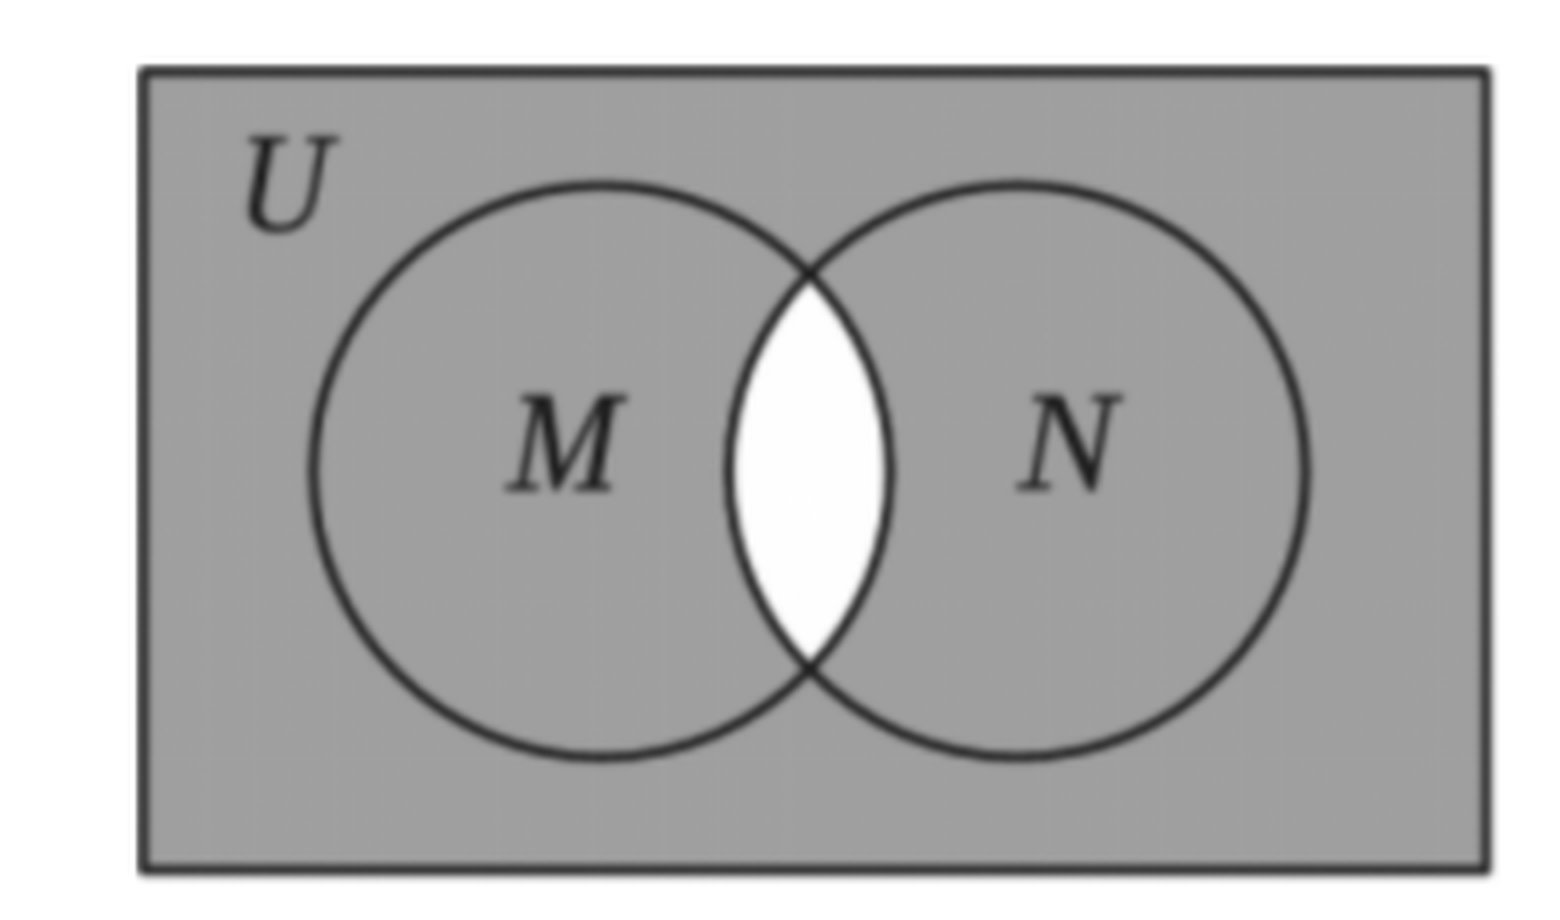
\includegraphics[width=0.40\textwidth]{figures/gao145_q14.png}
\end{center}

\ifanswer
\solbegin
\step{由韦恩图得图中白色区域为集合 $M\cap N$，所以阴影部分表示的集合为 $\overline{M\cap N}$.}
\step{故选 $D$.}
\solend
\fi

% === Q15 ===
\item 已知 $x>-2$，则 $x+\dfrac{1}{x+2}$ 的最小值为\mbox{（\quad）}

\keepwithprev
A. 3\qquad B. 2\qquad C. 1\qquad D. 0

\ifanswer
\solbegin
\step{$x>-2$，则 $x+2>0$，}
\step{所以 $x+\dfrac{1}{x+2}=(x+2)+\dfrac{1}{x+2}-2\geqslant2\sqrt{(x+2)\cdot\dfrac{1}{x+2}}-2=0$，}
\step{当且仅当 $x+2=\dfrac{1}{x+2}$，即 $x=-1$ 时取等号，所以 $x+\dfrac{1}{x+2}$ 的最小值为 $0$.}
\step{故选 $D$.}
\solend
\fi

% 第 16 题：题干在 05 页、解析续至 06 页；两幅数轴标根波浪曲线是【解析】内配图，
% 仅答案版出，放在答案版条件块内 \solbegin 的 \step 之间（照 高一73 第 16 题成例）
\item 关于 $x$ 的不等式 $\dfrac{(x-a)(x-2)^2}{(x-1)(x-5)}\leqslant0$ 的解集中恰有 3 个正整数，则实数 $a$ 的取值范围是\mbox{（\quad）}

\keepwithprev
A. $(-\infty,3]\cup[7,8)$\qquad B. $(-\infty,3)\cup[7,8)$\qquad C. $(-\infty,3]\cup(7,8]$\qquad D. $(-\infty,3)\cup(7,8]$

\ifanswer
\solbegin
\step{由题意，不等式 $\dfrac{(x-a)(x-2)^2}{(x-1)(x-5)}\leqslant0$，}
\step{可化为 $\begin{cases}(x-1)(x-2)^2(x-5)(x-a)\leqslant0\\x\ne1\text{且}x\ne5\end{cases}$，由数轴标根法，}
\step{当 $a=3$ 时，}
\begin{center}
% a=3 数轴标根图取 06 页，去粉色水印、去色、4× LANCZOS 放大；仅答案版出
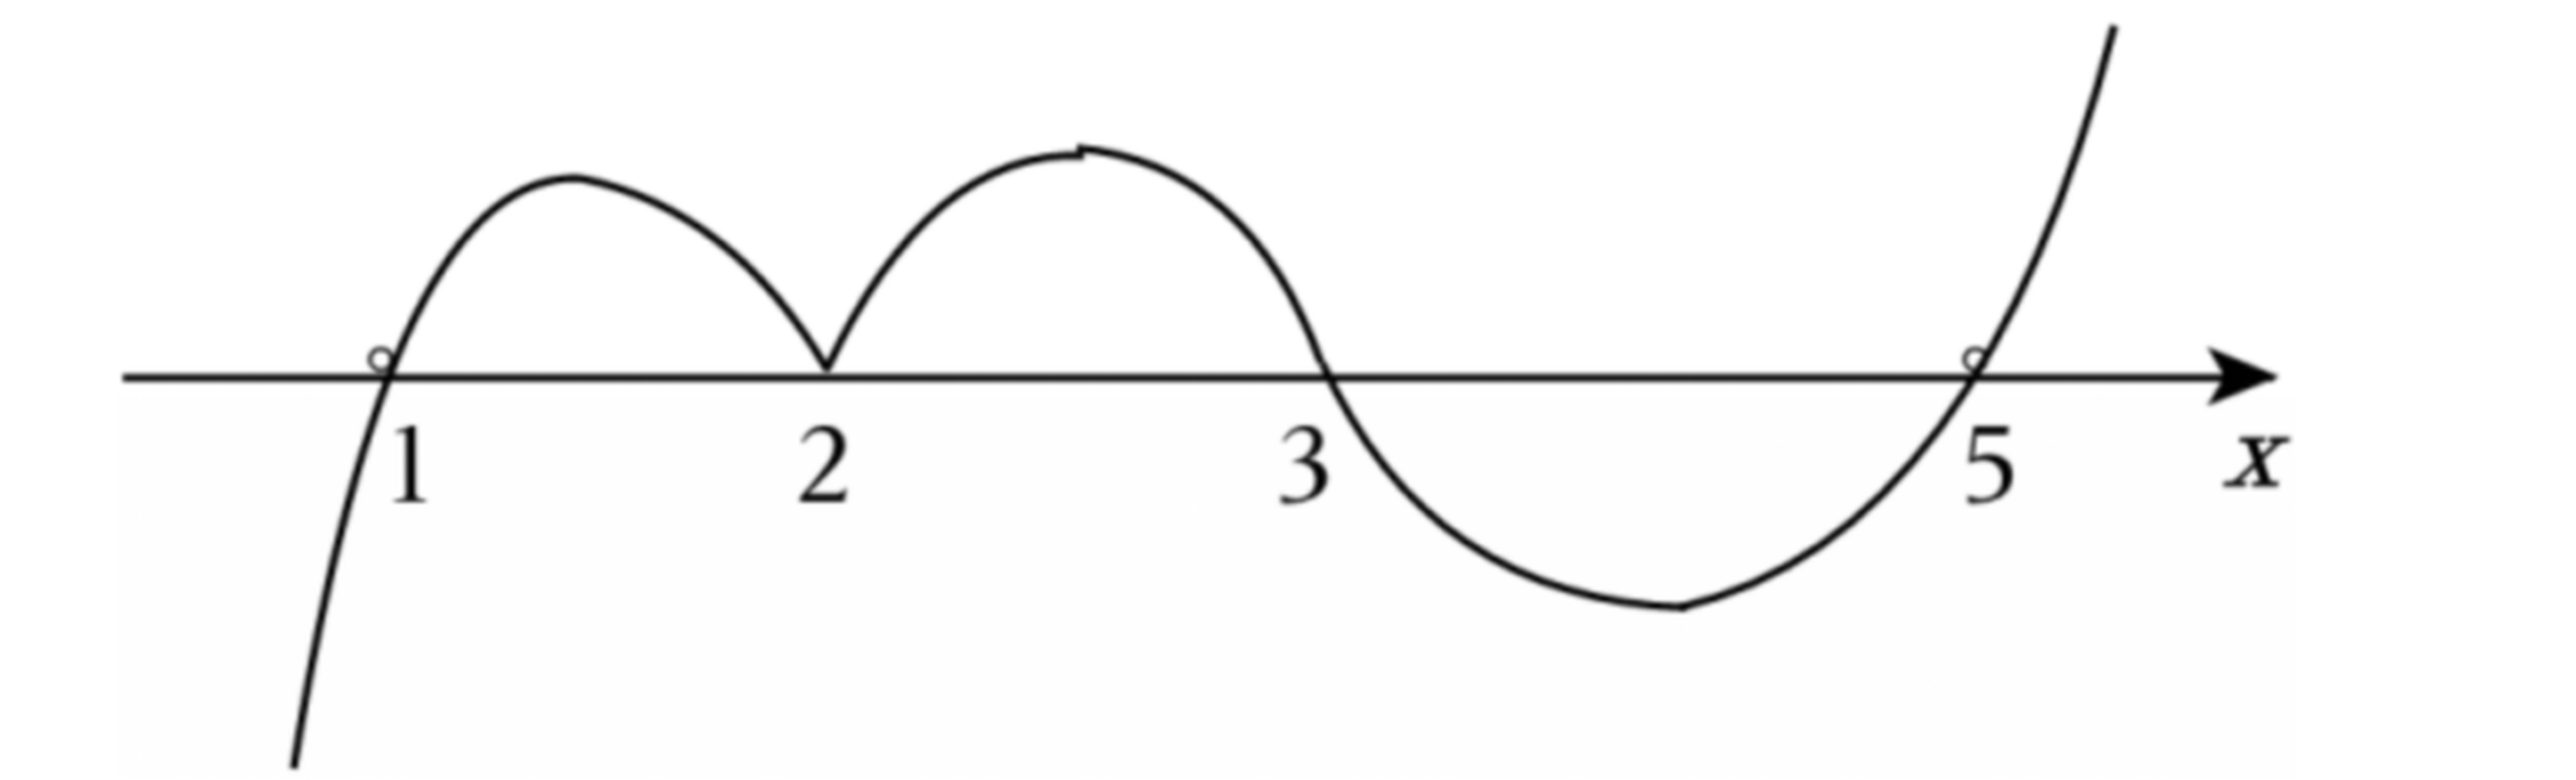
\includegraphics[width=0.62\textwidth]{figures/gao145_q16_a3.png}
\end{center}
\step{得不等式的解集为 $\{x\mid x<1\text{ 或 }x=2\text{ 或 }3\leqslant x<5\}$，}
\step{对应的正整数解为 $2$，$3$，$4$，满足题意，故排除 $B$、$D$；}
\step{当 $a=7$ 时，}
\begin{center}
% a=7 数轴标根图取 06 页，去粉色水印、去色、4× LANCZOS 放大；仅答案版出
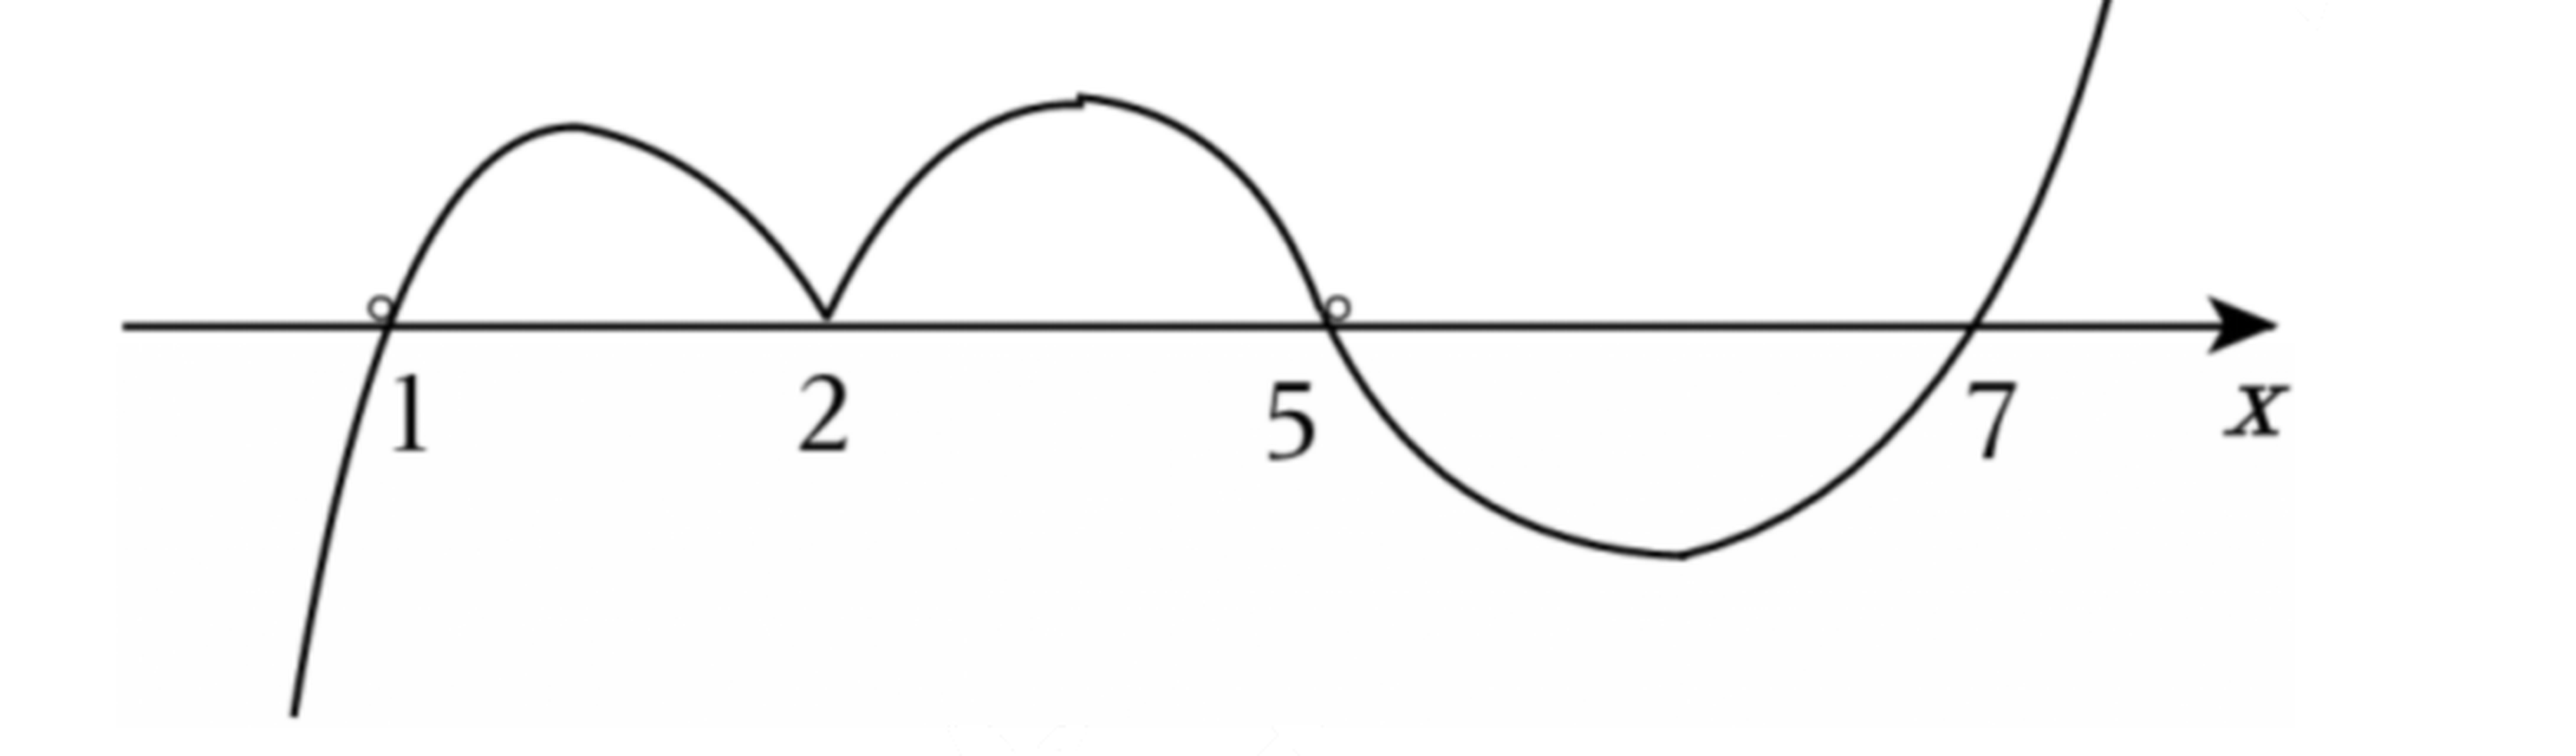
\includegraphics[width=0.62\textwidth]{figures/gao145_q16_a7.png}
\end{center}
\step{得不等式的解集为 $\{x\mid x<1\text{ 或 }x=2\text{ 或 }5<x\leqslant7\}$，}
\step{对应的正整数解为 $2$，$6$，$7$，满足题意，故 $A$ 正确，$C$ 错误.}
\step{故选 $A$.}
\solend
\fi

\end{enumerate}

\bigsec{三、解答题}

\begin{enumerate}
\setcounter{enumi}{16}

% 第 17 题：题干在 06 页、解析续至 07 页，按印刷行断，共 7 行；
% "lg(10÷5)" 的除号照录 \div
\item (1) 已知 $a+a^{-1}=6$，求 $a^2+a^{-2}$ 及 $a^{\frac12}-a^{-\frac12}$ 的值；

(2) 已知 $\lg5=a$，$\lg6=b$，用 $a$、$b$ 分别表示 $\lg2$、$\lg3$、$\lg300$ 和 $\log_{12}15$.

\ifanswer
\solbegin
\step{(1) 因为 $a+a^{-1}=6$，}
\step{所以 $a^2+a^{-2}=(a+a^{-1})^2-2\cdot a\cdot a^{-1}=6^2-2=34$，}
\step{因为 $\left(a^{\frac12}-a^{-\frac12}\right)^2=a-2+a^{-1}=6-2=4$，所以 $a^{\frac12}-a^{-\frac12}=\pm2$；}
\step{(2) $\lg2=\lg(10\div5)=\lg10-\lg5=1-a$，}
\step{$\lg3=\lg(6\div2)=\lg6-\lg2=b-(1-a)=a+b-1$，}
\step{$\lg300=\lg(3\times10^2)=\lg3+\lg10^2=a+b-1+2=a+b+1$，}
\step{所以 $\log_{12}15=\dfrac{\lg15}{\lg12}=\dfrac{\lg3+\lg5}{\lg3+\lg2^2}=\dfrac{a+b-1+a}{a+b-1+2(1-a)}=\dfrac{2a+b-1}{b-a+1}$.}
\solend
\fi

% 第 18 题：题干在 07 页、解析续至 08 页（2 问、分类讨论很长），按印刷行断共 25 行；
% 本卷 Q18 用"图像"（Q13/Q14 用"图象"），逐处照录不统一
\item 已知 $f(x)=(m^2-3m+1)x^{m^2-4m-1}$，$y=f(x)$ 为幂函数且在 $(0,+\infty)$ 上是严格减函数.

(1) 求实数 $m$ 的值以及相应的函数表达式；

(2) 若 $y=f(x)$ 的图像关于 $y$ 轴对称，解关于 $x$ 的不等式 $(x+2)^{1-m}<(3x-1)^{1-m}$.

\ifanswer
\solbegin
\step{(1) 由幂函数的定义得 $m^2-3m+1=1$，}
\step{整理得 $m^2-3m=0$，解得 $m=0$ 或 $m=3$，}
\step{由于 $y=f(x)$ 在 $(0,+\infty)$ 上为严格减函数，}
\step{因此幂函数的指数需满足 $m^2-4m-1<0$，}
\step{当 $m=3$ 时，指数为 $3^2-4\times3-1=-4<0$，满足严格递减条件，}
\step{此时函数表达式为 $f(x)=x^{-4}$，}
\step{当 $m=0$ 时，指数为 $0^2-4\times0-1=-1<0$，满足严格递减条件，}
\step{此时函数表达式为 $f(x)=x^{-1}$，}
\step{所以满足条件的实数 $m$ 为 $0$ 或 $3$，}
\step{对应的函数表达式分别为 $f(x)=x^{-1}$、$f(x)=x^{-4}$；}
\step{(2) 函数图像关于 $y$ 轴对称即函数为偶函数，}
\step{对于 $f(x)=x^{-1}=\dfrac1x$，定义域为 $(-\infty,0)\cup(0,+\infty)$，}
\step{满足 $f(-x)=-f(x)$，为奇函数，图像关于原点对称，}
\step{不满足关于 $y$ 轴对称的条件；}
\step{对于 $f(x)=x^{-4}=\dfrac{1}{x^4}$，定义域为 $(-\infty,0)\cup(0,+\infty)$，}
\step{满足 $f(-x)=f(x)$，为偶函数，图像关于 $y$ 轴对称，}
\step{因此符合条件的 $m$ 值为 $3$，}
\step{将 $m=3$ 代入关于 $x$ 的不等式 $(x+2)^{1-m}<(3x-1)^{1-m}$，}
\step{得 $(x+2)^{1-3}<(3x-1)^{1-3}$，即 $(x+2)^{-2}<(3x-1)^{-2}$，}
\step{因为负指数幂的底数不能为 $0$，所以 $x+2\ne0$ 且 $3x-1\ne0$，}
\step{即 $x\ne-2$ 且 $x\ne\dfrac13$，}
\step{不等式可变形为 $\dfrac{1}{(x+2)^2}<\dfrac{1}{(3x-1)^2}$，}
\step{整理得 $(3x-1)^2<(x+2)^2$，即 $8x^2-10x-3<0$，}
\step{解得 $-\dfrac14<x<\dfrac32$，又 $x\ne-2$ 且 $x\ne\dfrac13$，}
\step{所以不等式的解集为 $\left(-\dfrac14,\dfrac13\right)\cup\left(\dfrac13,\dfrac32\right)$.}
\solend
\fi

% 第 19 题：题干在 08 页、解析续至 09 页，按印刷行断，共 14 行；
% 判别式 cases 块内"△=4a²−16a<0"原卷印扁等边三角 \triangle
%（放大 09 页 zz09_delta.png 与 Q12 高 \Delta 并排确认），逐处照录不统一
\item 已知 $f(x)=ax^2+2ax+4$，$a\in\R$.

(1) 若关于 $x$ 的不等式 $f(x)>0$ 在实数集 $\R$ 上恒成立，求实数 $a$ 的取值范围；

(2) 当 $a<0$ 时，解关于 $x$ 的不等式 $f(x)>(a+1)x+5$.

\ifanswer
\solbegin
\step{(1) 由题意得，关于 $x$ 的不等式 $f(x)>0$ 在实数集 $\R$ 上恒成立，}
\step{即 $ax^2+2ax+4>0$ 在实数集 $\R$ 上恒成立，}
\step{当 $a=0$ 时，不等式为 $4>0$ 恒成立，符合题意；}
\step{当 $a\ne0$ 时，则 $\begin{cases}a>0\\\triangle=4a^2-16a<0\end{cases}$，解得 $0<a<4$.}% 判别式原卷印扁等边三角 $\triangle$，照录
\step{综上所述，实数 $a$ 的取值范围为 $[0,4)$.}
\step{(2) $f(x)=ax^2+2ax+4$，}
\step{当 $a<0$ 时，不等式 $f(x)>(a+1)x+5$ 即为 $ax^2+(a-1)x-1>0$，}
\step{即 $(ax-1)(x+1)>0$，即 $\left(x-\dfrac1a\right)(x+1)<0$，}
\step{当 $a<-1$，即 $\dfrac1a>-1$ 时，解得 $-1<x<\dfrac1a$；}
\step{当 $a=-1$，即 $\dfrac1a=-1$ 时，解得 $x\in\varnothing$；}
\step{当 $-1<a<0$，即 $\dfrac1a<-1$ 时，解得 $\dfrac1a<x<-1$.}
\step{综上所述，当 $a<-1$ 时，不等式的解集为 $\left\{x\mid -1<x<\dfrac1a\right\}$；}
\step{当 $a=-1$ 时，不等式的解集为 $\varnothing$；}
\step{当 $-1<a<0$ 时，不等式的解集为 $\left\{x\mid \dfrac1a<x<-1\right\}$.}
\solend
\fi

% 第 20 题：菜园靠墙图为题目配图（三版都出），题干写"如图"；
% 题干在 09 页（含图）、解析续至 10 页，按印刷行断，共 13 行
\needvspace{8cm}
\item 如图，某人计划用篱笆围成一个一边靠墙（墙足够长）的矩形菜园. 设菜园的长为 $x$ 米，宽为 $y$ 米.

\begin{center}
% 矩形菜园靠墙图取 09 页右下，去粉色水印、去色、4× LANCZOS 放大
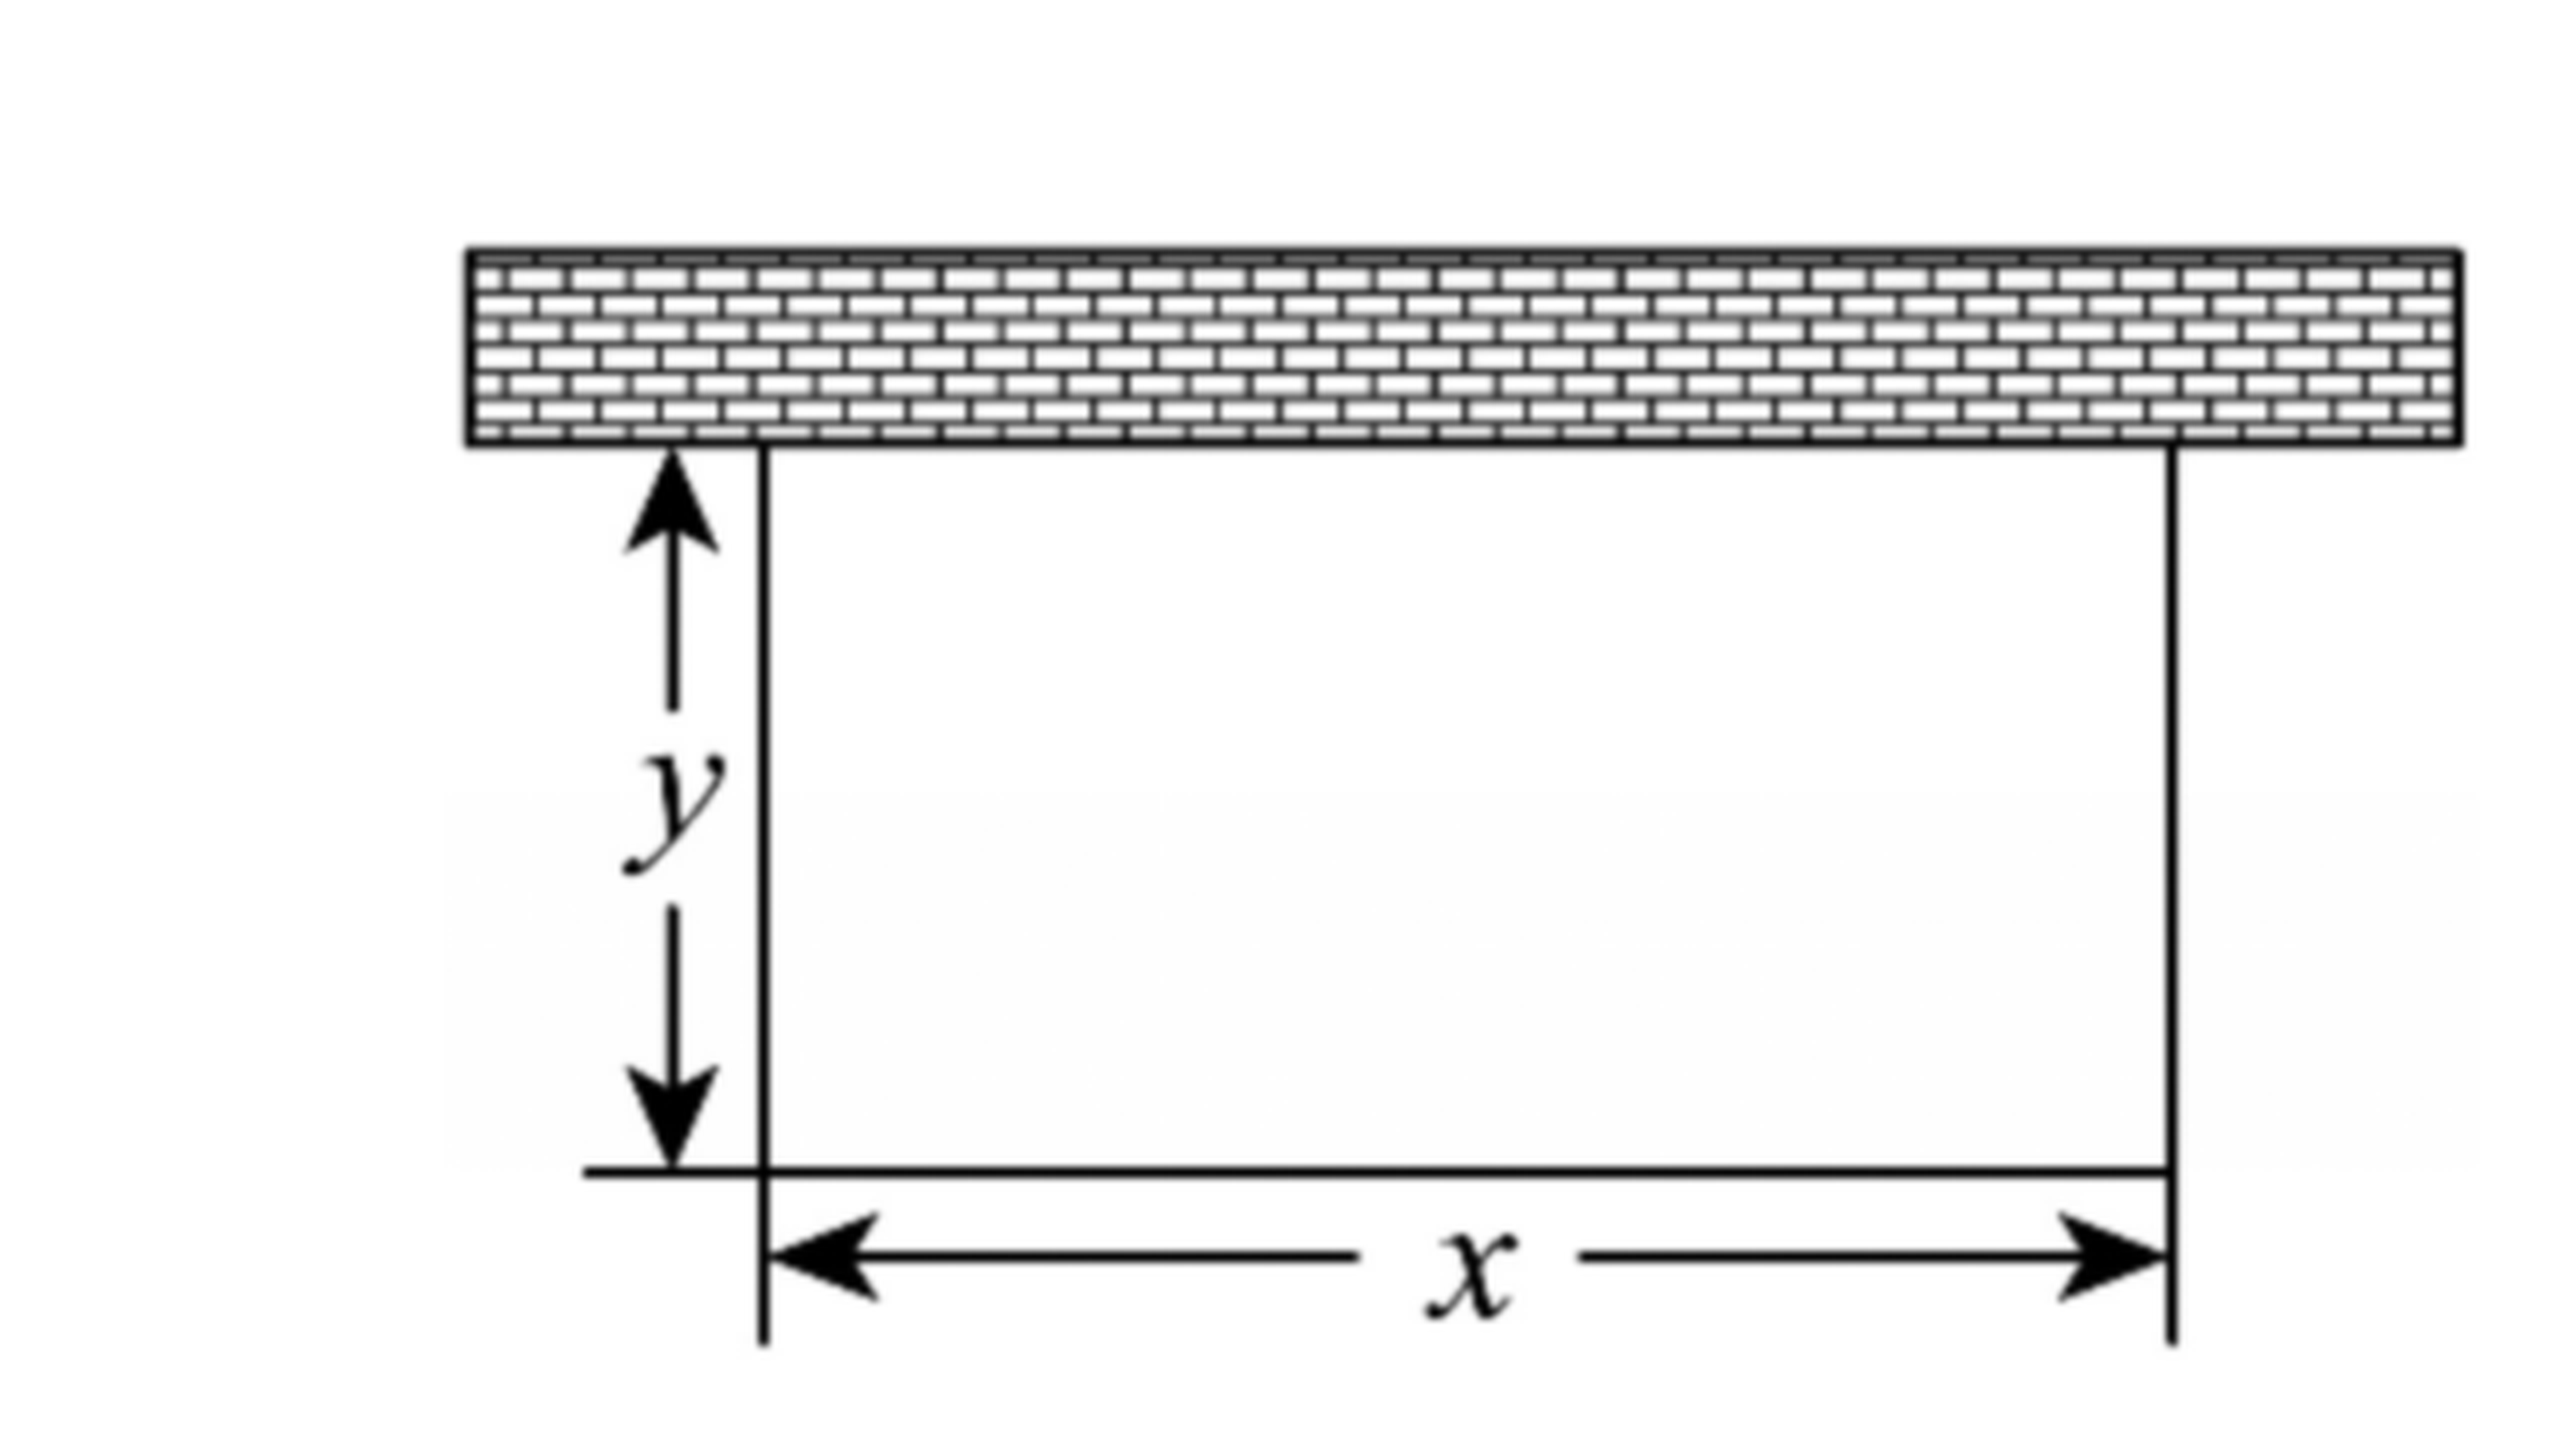
\includegraphics[width=0.55\textwidth]{figures/gao145_q20.png}
\end{center}

(1) 若菜园面积为 72 平方米，则 $x$、$y$ 为何值时，所用篱笆总长最小？

(2) 若 $x$、$y$ 满足 $x+y-xy+63=0$，则菜园面积最小为多少平方米？

\ifanswer
\solbegin
\step{(1) 由题意得，菜园的面积 $S=xy=72$，且 $x>0$，$y>0$，}
\step{所用篱笆总长 $L=x+2y$，}
\step{由基本不等式得 $x+2y\geqslant2\sqrt{x\cdot2y}=2\sqrt{2xy}=2\sqrt{2\times72}=24$，}
\step{当且仅当 $x=2y$ 时取等号，}
\step{联立 $\begin{cases}xy=72\\x=2y\end{cases}$，解得 $\begin{cases}x=12\\y=6\end{cases}$，}
\step{所以当 $x=12$，$y=6$ 时，所用篱笆总长最小；}
\step{(2) 由题意得 $x>0$，$y>0$，且满足 $x+y-xy+63=0$，即 $x+y=xy-63$，}
\step{由基本不等式得 $x+y\geqslant2\sqrt{xy}$，当且仅当 $x=y$ 时取等号，}
\step{所以 $xy-63\geqslant2\sqrt{xy}$. 令 $t=\sqrt{xy}(t>0)$，则 $xy=t^2$，}
\step{上述不等式可化为 $t^2-2t-63\geqslant0$，即 $(t-9)(t+7)\geqslant0$，}
\step{因为 $t>0$，所以 $t+7>0$，故 $t-9\geqslant0$，解得 $t\geqslant9$，所以 $\sqrt{xy}\geqslant9$，}
\step{即 $xy\geqslant81$，当且仅当 $x=y=9$ 时取等号，此时满足 $9+9-81+63=0$，}
\step{所以菜园面积最小为 81 平方米.}
\solend
\fi

% 第 21 题：题干在 10 页、解析续至 11 页（3 问、分类讨论很长），按印刷行断共 22 行；
% 末行"故第 2026 个元素是 2700 之后第一个属于 A 的数，即 2701." 为全卷收尾，
% 无 Q22/Q23、无附加题节；数集 Z/N* 按全稿惯例改 \Z/\N^*
\item 已知集合 $A=\{x\mid x=m^2-n^2$，$m$、$n\in\Z\}$.

(1) 求证：任何奇数 $2k+1(k\in\Z)$ 都是集合 $A$ 中的元素；

(2) 判断偶数 $4k-2(k\in\Z)$ 是否为集合 $A$ 的元素？请说明理由；

(3) 若将集合 $A$ 中的正整数由小到大排列，求出集合 $A$ 中第 2026 个正整数.

\ifanswer
\solbegin
\step{(1) 因为 $x=(k+1)^2-k^2=2k+1(k\in\Z)$，}
\step{所以任何奇数 $2k+1(k\in\Z)$ 都属于集合 $A$；}
\step{(2) 偶数 $4k-2(k\in\Z)$ 不是集合 $A$ 的元素，理由如下：}
\step{由题意得 $x=m^2-n^2=(m-n)(m+n)$，}
\step{当 $m$、$n$ 均为奇数时，设 $m=2k_1+1$，$n=2k_2+1(k_1$、$k_2\in\Z)$，}
\step{则 $m^2-n^2=(2k_1+1)^2-(2k_2+1)^2=(2k_1-2k_2)(2k_1+2k_2+2)$}
\step{$=4(k_1-k_2)(k_1+k_2+1)$，}
\step{因为 $k_1$、$k_2\in\Z$，所以 $k_1-k_2\in\Z$，$k_1+k_2+1\in\Z$，}
\step{从而 $m^2-n^2$ 为 $4$ 的倍数；}
\step{当 $m$、$n$ 均为偶数时，设 $m=2k_1$，$n=2k_2(k_1$、$k_2\in\Z)$，}
\step{$m^2-n^2=4k_1^2-4k_2^2=4(k_1^2-k_2^2)$ 为 $4$ 的倍数；}
\step{当 $m$、$n$ 为一个偶数一个奇数时，不妨设 $m$ 为偶数，$n$ 为奇数，}
\step{设 $m=2k_1$，$n=2k_2+1(k_1$、$k_2\in\Z)$，}
\step{则 $m^2-n^2=4k_1^2-(2k_2+1)^2=4(k_1^2-k_2^2-k_2)-1$ 为奇数.}
\step{无论哪种情况均不满足 $4k-2(k\in\Z)$，}
\step{故偶数 $4k-2(k\in\Z)$ 不是集合 $A$ 的元素；}
\step{(3) 由前两问得，$4$ 的倍数和奇数属于集合 $A$ 中的元素，}
\step{令集合 $A$ 中的正整数元素为 $4k-3$、$4k-1$、$4k(k\in\N^*)$，}
\step{对任意的 $k\in\N^*$，连续的 $4$ 个整数 $4k-3$、$4k-2$、$4k-1$、$4k$ 中}
\step{有三个数 $4k-3$、$4k-1$、$4k$ 都在集合 $A$ 中，}
\step{因为 $2026=3\times675+1$，所以集合 $A$ 中第 $2025$ 个元素为 $4\times675=2700$，}
\step{故第 2026 个元素是 2700 之后第一个属于 $A$ 的数，即 2701.}
\solend
\fi

\end{enumerate}

\end{document}
"
%
% ① 原始材料：微信公众号"魔都数学加油站"文章，连载"27学年高一145"，原文标题
% "27学年高一145——2026-2027年上海市市二中学高一上期中"；
% 原文链接：https://mp.weixin.qq.com/s/6V-i9KE0GWodC-wmd5z8nQ 。
% 正文为 11 张 PNG 页（01/02/03/08/10/11 为 4762×6735，04/05/06/07/09 为 2560×3620，
% 同一篇各页分辨率不同，逐页按各自分辨率裁图核对，别按预览比例换算裁框）。
% 题目下印【答案】或【解析】，为混合体例讲评版：Q3 只印【答案】、无【解析】，其余
% 18 题印【解析】。题目、解析均据原图转录；卷面粉红色水印"魔都数学加油站"及
% 公众号页脚未录入。
% 全卷插图情况（逐页通读 11 页确认，题干写"如图"处均配有图）：
%   · Q14 韦恩图（05 页右侧，全集 U 矩形＋两圆 M/N＋白色交集、灰色阴影＋U/M/N 标注）：
%     题目配图（选择题选项旁），三版都出，裁自 05 页去水印去色 4× 放大存
%     figures/gao145_q14.png；
%   · Q16 两幅数轴标根波浪曲线（06 页，a=3 与 a=7 各一幅，标根法画
%     (x-1)(x-2)^2(x-5)(x-a)≤0 的符号曲线）：【解析】内的配图，仅答案版出，
%     裁 figures/gao145_q16_a3.png / figures/gao145_q16_a7.png（或合并一张），
%     放在答案版条件块内 \solbegin 的 \step 之间（照 高一73 第 16 题成例）；
%   · Q20 矩形菜园靠墙图（09 页右下，灰色砖墙＋矩形菜园＋x/y 标注＋箭头）：
%     题目配图，三版都出，裁自 09 页去水印去色 4× 放大存 figures/gao145_q20.png；
%   其余各页逐页确认无其它题目配图、无表格、亦无"题干写如图而源码漏图"一处。
%
% 卷首标题：原卷印作"2026-2027 年市二中学高一上期中"，年份区间按全稿惯例排 en dash；
% 原卷卷面未印副标题，本稿按同期中卷（高一140／141／143／144）知识模块口径补出
% "集合与常用逻辑用语、不等式、函数"。
%
% 题号体例：本卷共 19 题——一、填空题 3—12（10 题）、二、选择题 13—16（4 题）、
% 三、解答题 17—21（5 题）。三节分别 \setcounter{enumi}{2}／{12}／{16}。
% 原卷从第 3 题起、无第 1、2 题，本稿保留原题号；全卷无附加题节。
%
% ② 与原卷的排版差异：
%   ① 原文从第 3 题起，本稿保留原题号；共 19 题三节；
%   ② 混合体例：原卷 Q3 只印【答案】、无【解析】（"第一步应假设___。
%      【答案】x≤2 或 y≤2"），按 高一140 第 5 题成例提 \ans{}、不补造解析；
%      其余 18 题印【解析】，用 \solbegin…\solend，选择题答案在解析末句"故选 X"
%      （Q13 选 B、Q14 选 D、Q15 选 D、Q16 选 A，逐个放大原图核实）、
%      题干括号 \mbox{（\quad）} 留空、不另提 \ans{}；填空／解答答案落在解析里；
%      答案版【答案】/【解析】标记数 = 19（1 个 \ans ＋ 18 个 \solbegin）= 全卷题数；
%   ③ 原卷卷面未印副标题，本稿按知识模块口径补出；
%   ④ 原卷填空横线按全稿惯例排 \blankline[4.4em]；选择题括号排 \mbox{（\quad）}、
%      选项段前按惯例加 \keepwithprev；解答题不留作答区、不加 \anspace
%      （原卷为讲评版，与 129／131／132／133／136／140／141／143／144 同）；
%   ⑤ 数集：Q9"a、b∈R"、Q12"a∈R"、Q21"m、n∈Z""k∈Z""k∈N*"等原卷印
%      斜体或黑板粗体 R/Z/N，按全稿惯例统一改 \R／\Z／\N^*；绝对值排 \lvert…\rvert，
%      集合描述竖线排 \mid；不等号按全稿惯例排 \leqslant／\geqslant；
%      补集照原卷上划线排 \overline{M}／\overline{N}（Q14 选项 B/C/D 逐处核）；
%      空集记号 \varnothing；\subset（单线⊂）与 \subseteq（带下划线⊆）逐处照录不统一；
%   ⑥ 子题标号 (1)(2)(3) 原卷印半角括号照录；圈数字进数学式用 \text{①}（否则 FONTCHK 挂）；
%      \left…\right 不得拆到不同 $…$ 组；cases 块整体算一个印刷行；
%   ⑦ 题干／解析中的中文弯引号按原卷照录（Q3"若 x+y>4，则 x>2 且 y>2"、
%      Q11"a₁/a₂=b₁/b₂""M=N"、选填"充分非必要""必要非充分""充要""既非充分也非必要"
%      等，含引号内空格），注释内一律 ASCII 引号；数学式内 CJK 用 \text{}；
%   ⑧ 半角逗号在数学组之间是全稿惯例、非笔误（如 Q5"x₁+x₂=6，x₁x₂=√3"、
%      Q7"a>1，b>1"、指数／对数式内逗号），逐处照录别改全角；行末西文句点照录为
%      ASCII `.`；行中全角逗号／顿号照录；
%   ⑨ "图像／图象"逐处照录不统一（Q18"图像关于 y 轴对称"等，核全卷）；
%   ⑩ 判别式 Δ/△ 混用是照录项：Q12 解析"Δ=a²−4a²(2a−3)>0"、
%      Q19 解析"Δ=4a²−16a<0"等，放大原图判断是高 \Delta（等腰偏高、高>宽）
%      还是扁 \triangle，逐处照录不得统一（参照 高一142／144 头注④口径）；
%   ⑪ 一条 \step = 原卷解析的一个印刷行，cases 块整体算一个印刷行；别把原卷折行
%      并起来、别把一行拆多条。Q6 分段讨论、Q12 三个 cases 条件组、Q16 数轴标根、
%      Q18／Q19 分类讨论、Q21 三问均按印刷行逐条断，不丢行；
%   ⑫ Q14 韦恩图为"题干＋选项＋图"整块，加 \needvspace 守卫推走（守卫放 \item 之前，
%      见 高一140 Q14、高一144 Q17 成例与切页审计 B 类坑）；Q20 菜园图同理；
%      三版切页审计均"合计异常：无"；
%   ⑬ 跨页续印按题合并：Q3/4/5/6 在 01 页（Q6 解析续 02 页顶）；Q7/8/9/10 在 02 页
%      （Q10 解析续 03 页）；Q11/12 在 03 页（Q12 解析续 04 页，很长）；
%      Q13 在 04 页末、解析在 05 页顶；Q14/15/16 在 05 页（Q16 解析续 06 页含两幅数轴图）；
%      Q17 在 06 页、解析续 07 页；Q18 在 07 页、解析续 08 页；Q19 在 08 页、解析续 09 页；
%      Q20 在 09 页（含菜园图）、解析续 10 页；Q21 在 10 页、解析续 11 页
%      （末页收尾"故第 2026 个元素是 2700 之后第一个属于 A 的数，即 2701."、
%      无 Q22/Q23、无附加题节）。本稿按题连排，不丢行、不并折行；
%   ⑭ 原卷解析内若有红色"法一／法二"之类小标题，按全稿惯例排 \stepm{标签}{…}
%      （黑体着色、不引入红色、不改 common.sty），头注注明；水印"魔都数学加油站"
%      红色不录入。
%
% ③ 行数复核：一条 \step／\stepm = 原卷解析的一个印刷行，cases 块作一个印刷行计。
%   逐题数（主会话逐页核对定稿）：Q3：0（只印【答案】、提 \ans{}，不计入 \step 账）；
%   Q4：3；Q5：2；Q6：10；Q7：3；Q8：3；Q9：2；Q10：7；Q11：4；Q12：12；
%   Q13：2；Q14：2；Q15：4；Q16：9；Q17：7；Q18：25；Q19：14；Q20：13；Q21：22。
%   合计 144 条 \step（本卷无 \stepm：解析内无红色"法一／法二"类小标题），
%   与原卷逐题印刷行相等。全卷 18 题设 \solbegin…\solend ＋ Q3 一处 \ans{}，
%   答案版【答案】/【解析】标记数 = 19 = 全卷题数。
%
% ④ 判别式／子集符号结论（逐处放大原图照录、不得统一，主会话像素级复核）：
%   判别式全卷 2 处、两形混用逐处照录不统一（参照 高一142／144 头注④口径）：
%     · Q12 解析 cases 块"Δ=a²−4a²(2a−3)>0" 原卷印等腰偏高粗三角（高>宽），
%       照录 \Delta（放大 04 页 /tmp/gao145s2/main_q12_delta.png 确认）；
%     · Q19 解析 cases 块"△=4a²−16a<0" 原卷印扁等边空心三角（宽≈高、细线），
%       照录 \triangle（放大 09 页 /tmp/gao145s2/main_q19_delta.png 确认）。
%   子集／补集：Q14 选项 A `M\cup N`、B `M\cap\overline{N}`（上划线只在 N 上）、
%   C `\overline{M\cup N}`（罩整个 M∪N）、D `\overline{M\cap N}`（罩整个 M∩N，
%   非 \overline{M}\cap N；放大 05 页 /tmp/gao145s2/main_q14_opts.png 确认），
%   阴影为灰色区域＝全集减白色交集，答案 D，照录 \overline{M\cap N}；
%   全集卷无 \subset／\subseteq 混用（本卷集合题用 \cup／\cap／\overline{}）；
%   空集 \varnothing（Q19 解析 x∈\varnothing）；数集 \R／\Z／\N^* 归一见 ② ⑤。
%
% ⑤ 存疑照录（放大原图确认，照录未改、正文对应处另有 % 注）：
%   1. Q3 题干"若 x+y>4，则 x>2 且 y>2" 后"时"前留一空格、弯引号内空格照录；
%      该卷混合体例（Q3 只印【答案】、提 \ans{}）见 ② ②。
%   2. Q4／Q5 解析中的"1，3，5 和 6"、"x₁+x₂=6,x₁x₂=√3" 等半角／全角逗号
%      逐处照原卷（放大 01 页确认），数学式内半角逗号为全稿惯例、非笔误。
%   3. Q14 选项 D 上划线罩住整个 M∩N（而非仅罩 M），照录 \overline{M\cap N}。
%   4. Q12 判别式高 \Delta 与 Q19 判别式扁 \triangle 两形混用，逐处照录不统一（见 ④）。
%   全卷除此 4 类外未发现其它笔误／自相矛盾处。
%
% ⑥ 跨页续印按题合并说明：见 ② ⑬。
%
\documentclass[a4paper,11pt]{article}
\usepackage{common}

\begin{document}

\examtitlest[3]{2026--2027 年市二中学高一上期中}{集合与常用逻辑用语、不等式、函数}

\bigsec{一、填空题}

\begin{enumerate}
\setcounter{enumi}{2}

% 第 3 题：原卷只印【答案】、无【解析】（放大 01 页确认），按 高一140 第 5 题成例
% 提 \ans{}、不补造解析；题干中文弯引号与"时"前空格照录
\item 用反证法证明命题：“若 $x+y>4$，则 $x>2$ 且 $y>2$” 时，第一步应假设\blankline[4.4em].

\ifanswer
\ans{$x\leqslant2$ 或 $y\leqslant2$}
\fi

% === Q4 ===
\item 设集合 $M$ 满足 $\{1,3,5,6\}\cup M=\{1,2,3,4,5,6\}$，则满足条件的所有 $M$ 的个数为\blankline[4.4em].

\ifanswer
\solbegin
\step{集合 $M$ 满足 $\{1,3,5,6\}\cup M=\{1,2,3,4,5,6\}$，}
\step{则 $M$ 中必含有 $2$ 和 $4$，$1$，$3$，$5$ 和 $6$ 可以选也可不选，}
\step{则满足条件的所有 $M$ 的数目相当于集合 $\{1,3,5,6\}$ 的子集的个数 $2^4=16$.}
\solend
\fi

% === Q5 ===
\item 已知方程 $x^2-6x+\sqrt3=0$ 的两根为 $x_1$ 和 $x_2$，则 $(x_1-x_2)^2=$\blankline[4.4em].

\ifanswer
\solbegin
\step{因为方程 $x^2-6x+\sqrt3=0$ 的两根为 $x_1$ 和 $x_2$，所以 $x_1+x_2=6,x_1x_2=\sqrt3$，}% 数学式内半角逗号为全稿惯例，照录
\step{所以 $(x_1-x_2)^2=(x_1+x_2)^2-4x_1x_2=36-4\sqrt3$.}
\solend
\fi

% 第 6 题：题干在 01 页，解析续至 02 页顶（末 2 行），按印刷行逐条断，共 10 行
\item 不等式 $\lvert x-2026\rvert+\lvert x-2029\rvert>3$ 的解集是\blankline[4.4em].

\ifanswer
\solbegin
\step{当 $x<2026$ 时，$x-2026<0$，$x-2029<0$，}
\step{原不等式可化为 $(2026-x)+(2029-x)>3$，解得 $x<2026$，}
\step{故此时，不等式的解为 $x<2026$；}
\step{当 $2026\leqslant x\leqslant2029$ 时，$x-2026\geqslant0$，$x-2029\leqslant0$，}
\step{原不等式可化为 $(x-2026)+(2029-x)>3$，即 $3>3$，显然不成立，}
\step{故此时，不等式无解；}
\step{当 $x>2029$ 时，$x-2026>0$，$x-2029>0$，}
\step{原不等式可化为 $(x-2026)+(x-2029)>3$，解得 $x>2029$，}
\step{故此时，不等式的解为 $x>2029$.}
\step{综上，原不等式的解集为 $(-\infty,2026)\cup(2029,+\infty)$.}
\solend
\fi

% === Q7 ===
\item 已知 $a>1$，$b>1$，若 $\log_a b+\log_b a=2$，且 $ab=2$，则 $\log_2(a+b)=$\blankline[4.4em].

\ifanswer
\solbegin
\step{由 $\log_a b+\log_b a=2$，$a>1$，$b>1$，得 $\log_a b+\dfrac{1}{\log_a b}=2$，}
\step{即 $(\log_a b)^2-2\log_a b+1=0$，则 $(\log_a b-1)^2=0$，解得 $\log_a b=1$，即 $a=b$，}
\step{又 $ab=2$，所以 $a=b=\sqrt2$，所以 $\log_2(a+b)=\log_2 2\sqrt2=\log_2 2^{\frac32}=\dfrac32$.}
\solend
\fi

% === Q8 ===
\item 已知 $m>0$，$n>0$，且 $m+n=1$，则 $\dfrac1m+\dfrac4n$ 的最小值为\blankline[4.4em].

\ifanswer
\solbegin
\step{由 $m>0$，$n>0$，$m+n=1$，}
\step{则 $\dfrac1m+\dfrac4n=(m+n)\left(\dfrac1m+\dfrac4n\right)=5+\dfrac nm+\dfrac{4m}n\geqslant5+2\sqrt{\dfrac nm\cdot\dfrac{4m}n}=9$，}
\step{当且仅当 $n=2m=\dfrac23$ 时，上式取得等号，故最小值为 $9$.}
\solend
\fi

% === Q9 ===
\item 已知 $a$、$b\in\R$，且 $3a+2b=1$，则 $8^a+4^b$ 最小值为\blankline[4.4em].

\ifanswer
\solbegin
\step{因为 $3a+2b=1$，所以 $8^a+4^b=2^{3a}+2^{2b}\geqslant2\sqrt{2^{3a+2b}}=2\sqrt2$，}
\step{当且仅当 $3a=2b$ 时取等号，故最小值为 $2\sqrt2$.}
\solend
\fi

% 第 10 题：题干在 02 页、解析续至 03 页顶，按印刷行断，共 7 行
\item 已知关于 $x$ 的不等式 $ax^2+bx+c>0$ 的解集为 $\{x\mid 1<x<2\}$，则关于 $x$ 的不等式 $bx^2-ax+c<0$ 的解集为\blankline[4.4em].

\ifanswer
\solbegin
\step{已知关于 $x$ 的不等式 $ax^2+bx+c>0$ 的解集为 $\{x\mid 1<x<2\}$，}
\step{由解集为 $1<x<2$ 且二次函数在两根之间为正，得 $a<0$，两个根为 $1$，$2$，}
\step{所以 $ax^2+bx+c=a(x-1)(x-2)=ax^2-3ax+2a$，}
\step{比较系数得 $b=-3a$，$c=2a$.}
\step{于是 $bx^2-ax+c=-3ax^2-ax+2a=-a(3x-2)(x+1)$，}
\step{$a<0$，故 $bx^2-ax+c<0$ 等价于 $(3x-2)(x+1)<0$，解得 $-1<x<\dfrac23$，}
\step{故 $bx^2-ax+c<0$ 的解集为 $\left\{x\mid -1<x<\dfrac23\right\}$.}
\solend
\fi

% 第 11 题：题干引号内空格照录（放大 03 页确认），四组选填引号亦同；
% 结论"故为必要非充分条件"照录，解析共 4 个印刷行
\item 设 $a_1$、$b_1$、$a_2$、$b_2$ 均为非零实数，不等式 $a_1x+b_1>0$ 和 $a_2x+b_2>0$ 的解集分别为集合 $M$、$N$，那么 “ $\dfrac{a_1}{a_2}=\dfrac{b_1}{b_2}$ ” 是 “ $M=N$ ” 的\blankline[4.4em]条件（选填 “ 充分非必要 ”、“ 必要非充分 ”、“ 充要 ” 和 “ 既非充分也非必要 ”）.

\ifanswer
\solbegin
\step{当 $a_1=b_1=1$，$a_2=b_2=-1$ 时，满足 $\dfrac{a_1}{a_2}=\dfrac{b_1}{b_2}$，}
\step{但是 $M=N$ 不成立，即充分性不成立；}
\step{若 $M=N$ 时，$\dfrac{a_1}{a_2}=\dfrac{b_1}{b_2}$ 一定成立，即必要性成立.}
\step{故为必要非充分条件.}
\solend
\fi

% 第 12 题：题干在 03 页、解析续至 04 页（很长，含 3 个 cases 条件组），
% 按印刷行逐条断共 12 行；cases 块整体算一个印刷行
\item 已知 $f(x)=\dfrac{ax+3}{x-2}$（常数 $a\in\R$）. 函数 $y=f(x)$ 在区间 $[3,+\infty)$ 上是严格减函数，且函数值不恒为负. 若关于 $x$ 的方程 $f(x)=\dfrac{a}{ax-1}$ 有两个不相等的实数根 $x_1$ 和 $x_2$，则 $a$ 的取值范围是\blankline[4.4em].

\ifanswer
\solbegin
\step{$f(x)=\dfrac{ax+3}{x-2}=a+\dfrac{3+2a}{x-2}$，定义域 $(-\infty,2)\cup(2,+\infty)$，}
\step{由于 $y=f(x)$ 在区间 $[3,+\infty)$ 上是严格减函数，且函数值不恒为负，}
\step{所以 $\begin{cases}3+2a>0\\a+\dfrac{3+2a}{3-2}\geqslant0\end{cases}\Rightarrow a\geqslant-1$，}
\step{若关于 $x$ 的方程 $f(x)=\dfrac{a}{ax-1}$ 有两个不相等的实数根 $x_1$ 和 $x_2$，}
\step{则 $\dfrac{ax+3}{x-2}=\dfrac{a}{ax-1}$，即 $(ax+3)(ax-1)=a(x-2)$，$x\ne2$ 且 $ax-1\ne0$，}
\step{当 $a\ne0$ 且 $a\geqslant-1$ 时，$(ax+3)(ax-1)=a(x-2)$，$x\ne2$ 且 $ax-1\ne0$，}
\step{可化为 $\begin{cases}a^2x^2+ax+2a-3=0\\x\ne2,x\ne\dfrac1a\end{cases}$，}
\step{要使方程有两个不相等的实数根 $x_1$ 和 $x_2$，}
\step{则 $\begin{cases}\Delta=a^2-4a^2(2a-3)>0\\a\geqslant-1\text{且}a\ne0\\4a^2+2a+2a-3\ne0\\a^2\cdot\dfrac1{a^2}+a\cdot\dfrac1a+2a-3\ne0\end{cases}\Rightarrow\begin{cases}a<\dfrac{13}{8}\\a\geqslant-1\text{且}a\ne0\\a\ne\dfrac12\text{且}a\ne-\dfrac32\\a\ne\dfrac12\end{cases}$，}% 判别式原卷印等腰偏高三角 $\Delta$，照录（放大 04 页 zz04_delta.png 确认）
\step{得 $-1\leqslant a<\dfrac{13}{8}$ 且 $a\ne0,a\ne\dfrac12$；}
\step{当 $a=0$ 时，方程无解；}
\step{所以 $a$ 的取值范围是 $[-1,0)\cup\left(0,\dfrac12\right)\cup\left(\dfrac12,\dfrac{13}{8}\right)$.}
\solend
\fi

\end{enumerate}

\bigsec{二、选择题}

\begin{enumerate}
\setcounter{enumi}{12}

% 第 13 题：题干在 04 页末、解析在 05 页顶；"图象"照录（本卷 Q13、Q14 用"图象"）
\item 已知幂函数 $f(x)$ 的图象过点 $\left(7,\dfrac{1}{\sqrt7}\right)$，则 $f(x)=$\mbox{（\quad）}

\keepwithprev
A. $x^{-2}$\qquad B. $x^{-\frac12}$\qquad C. $x^{\frac12}$\qquad D. $x^2$

\ifanswer
\solbegin
\step{设幂函数 $f(x)=x^\alpha(\alpha\in\R)$，因为幂函数的图象过点 $\left(7,\dfrac{1}{\sqrt7}\right)$，}
\step{所以 $7^\alpha=\dfrac{1}{\sqrt7}=7^{-\frac12}$，所以 $\alpha=-\dfrac12$，故 $f(x)=x^{-\frac12}$. 故选 $B$.}
\solend
\fi

% 第 14 题：韦恩图为题目配图（三版都出），"题干＋选项＋图"整块，needvspace
% 守卫放在 \item 之前（Q14 为选择题节内第二题，不会让节标题孤落页末）；
% D 选项上划线罩住整个 M∩N（放大 05 页 zz05_q14D.png 确认，非 \overline{M}\cap N）
\needvspace{9cm}
\item 已知全集 $U$ 和集合 $M$、$N$，用集合语言表示图中的阴影部分，正确的是\mbox{（\quad）}

\keepwithprev
A. $M\cup N$\qquad B. $M\cap\overline{N}$\qquad C. $\overline{M\cup N}$\qquad D. $\overline{M\cap N}$

\begin{center}
% 韦恩图取 05 页右侧，去粉色水印、去色、4× LANCZOS 放大
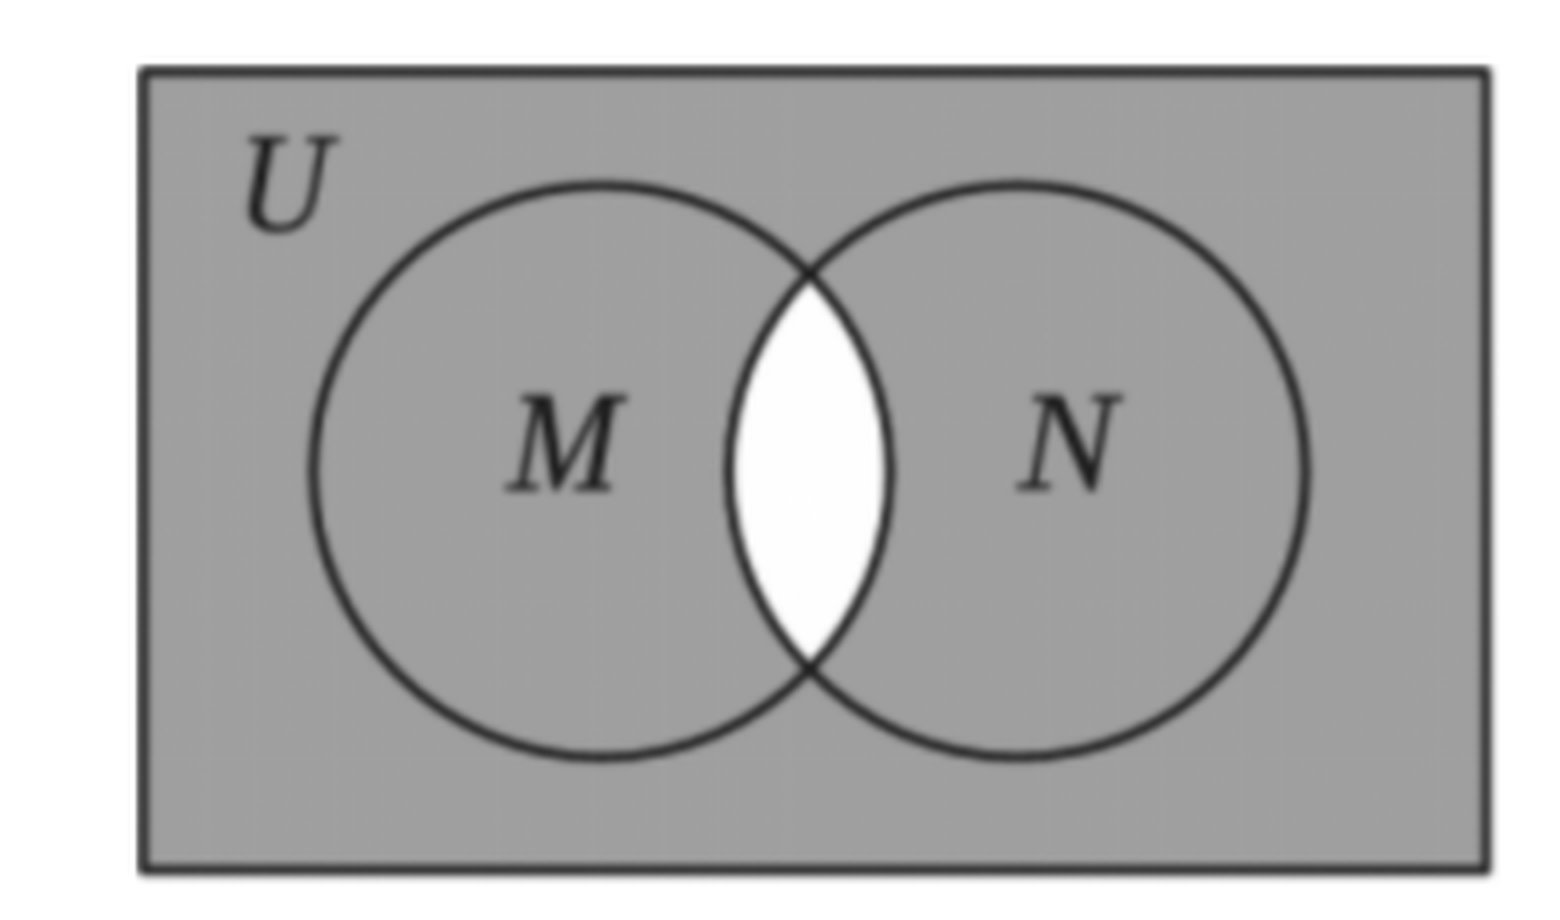
\includegraphics[width=0.40\textwidth]{figures/gao145_q14.png}
\end{center}

\ifanswer
\solbegin
\step{由韦恩图得图中白色区域为集合 $M\cap N$，所以阴影部分表示的集合为 $\overline{M\cap N}$.}
\step{故选 $D$.}
\solend
\fi

% === Q15 ===
\item 已知 $x>-2$，则 $x+\dfrac{1}{x+2}$ 的最小值为\mbox{（\quad）}

\keepwithprev
A. 3\qquad B. 2\qquad C. 1\qquad D. 0

\ifanswer
\solbegin
\step{$x>-2$，则 $x+2>0$，}
\step{所以 $x+\dfrac{1}{x+2}=(x+2)+\dfrac{1}{x+2}-2\geqslant2\sqrt{(x+2)\cdot\dfrac{1}{x+2}}-2=0$，}
\step{当且仅当 $x+2=\dfrac{1}{x+2}$，即 $x=-1$ 时取等号，所以 $x+\dfrac{1}{x+2}$ 的最小值为 $0$.}
\step{故选 $D$.}
\solend
\fi

% 第 16 题：题干在 05 页、解析续至 06 页；两幅数轴标根波浪曲线是【解析】内配图，
% 仅答案版出，放在答案版条件块内 \solbegin 的 \step 之间（照 高一73 第 16 题成例）
\item 关于 $x$ 的不等式 $\dfrac{(x-a)(x-2)^2}{(x-1)(x-5)}\leqslant0$ 的解集中恰有 3 个正整数，则实数 $a$ 的取值范围是\mbox{（\quad）}

\keepwithprev
A. $(-\infty,3]\cup[7,8)$\qquad B. $(-\infty,3)\cup[7,8)$\qquad C. $(-\infty,3]\cup(7,8]$\qquad D. $(-\infty,3)\cup(7,8]$

\ifanswer
\solbegin
\step{由题意，不等式 $\dfrac{(x-a)(x-2)^2}{(x-1)(x-5)}\leqslant0$，}
\step{可化为 $\begin{cases}(x-1)(x-2)^2(x-5)(x-a)\leqslant0\\x\ne1\text{且}x\ne5\end{cases}$，由数轴标根法，}
\step{当 $a=3$ 时，}
\begin{center}
% a=3 数轴标根图取 06 页，去粉色水印、去色、4× LANCZOS 放大；仅答案版出
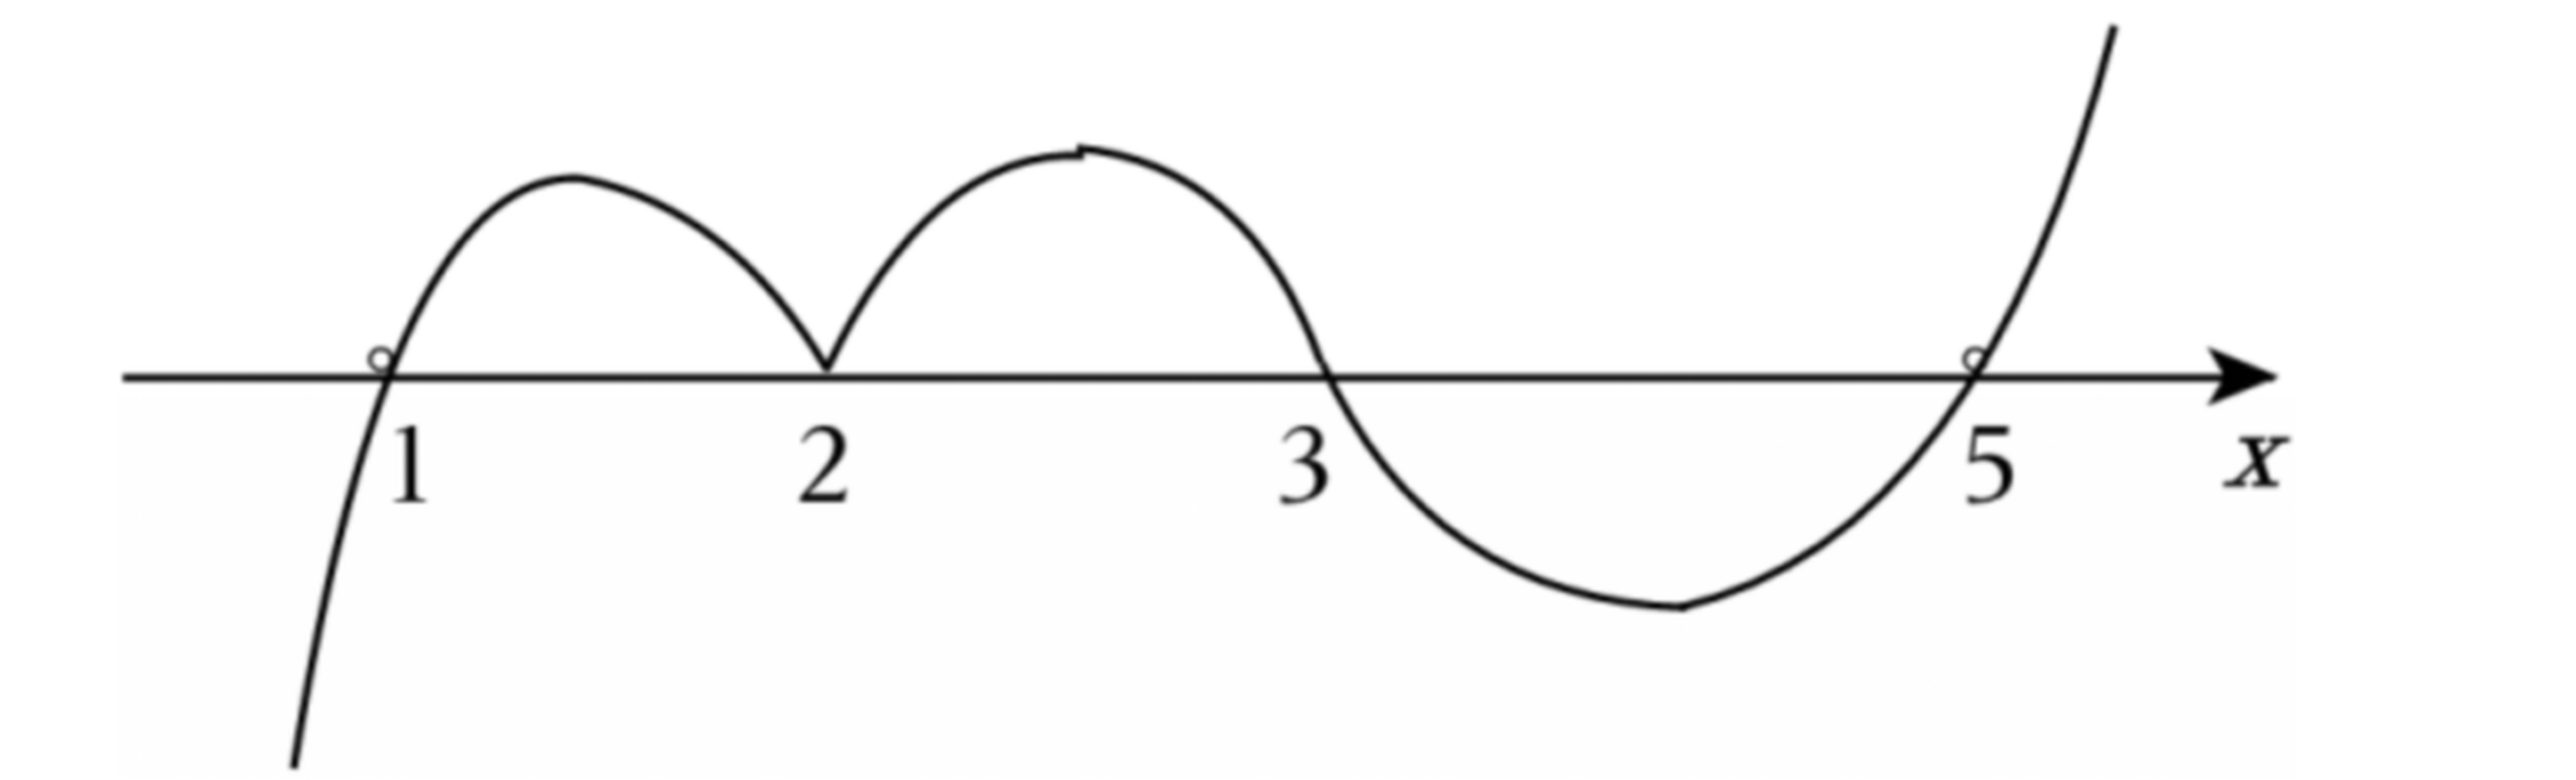
\includegraphics[width=0.62\textwidth]{figures/gao145_q16_a3.png}
\end{center}
\step{得不等式的解集为 $\{x\mid x<1\text{ 或 }x=2\text{ 或 }3\leqslant x<5\}$，}
\step{对应的正整数解为 $2$，$3$，$4$，满足题意，故排除 $B$、$D$；}
\step{当 $a=7$ 时，}
\begin{center}
% a=7 数轴标根图取 06 页，去粉色水印、去色、4× LANCZOS 放大；仅答案版出
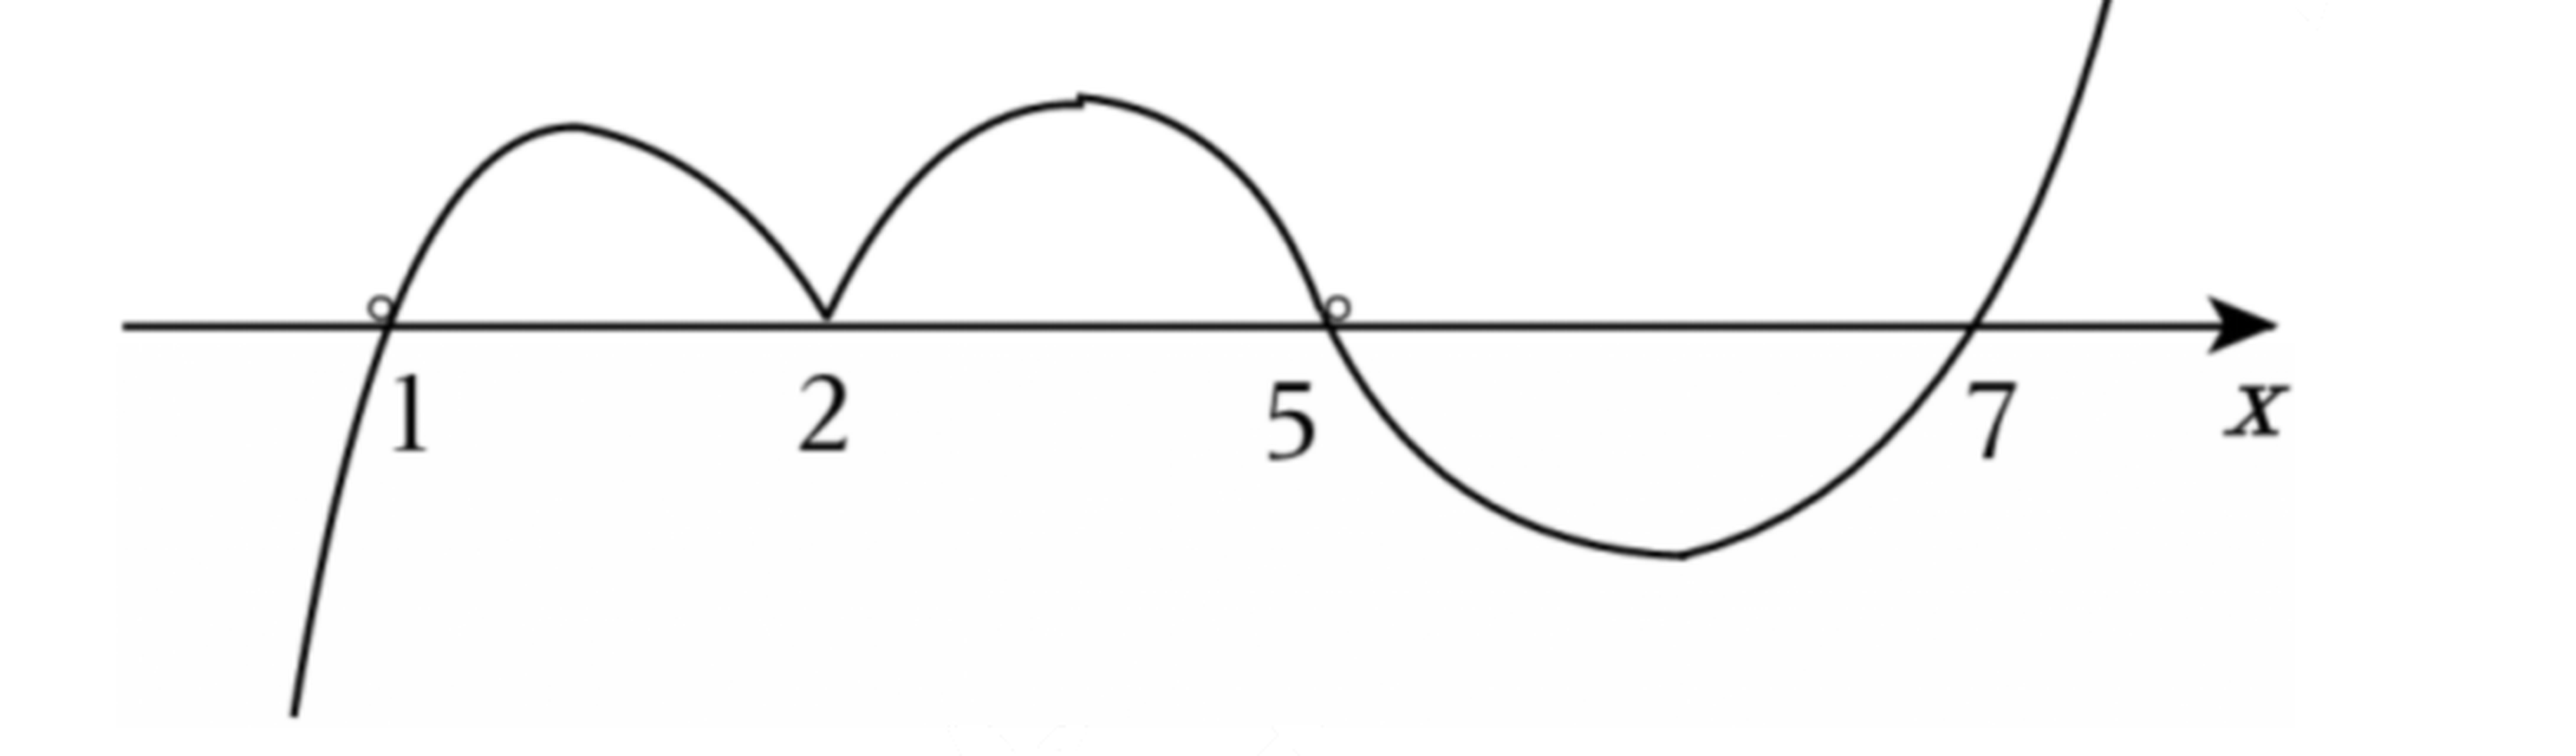
\includegraphics[width=0.62\textwidth]{figures/gao145_q16_a7.png}
\end{center}
\step{得不等式的解集为 $\{x\mid x<1\text{ 或 }x=2\text{ 或 }5<x\leqslant7\}$，}
\step{对应的正整数解为 $2$，$6$，$7$，满足题意，故 $A$ 正确，$C$ 错误.}
\step{故选 $A$.}
\solend
\fi

\end{enumerate}

\bigsec{三、解答题}

\begin{enumerate}
\setcounter{enumi}{16}

% 第 17 题：题干在 06 页、解析续至 07 页，按印刷行断，共 7 行；
% "lg(10÷5)" 的除号照录 \div
\item (1) 已知 $a+a^{-1}=6$，求 $a^2+a^{-2}$ 及 $a^{\frac12}-a^{-\frac12}$ 的值；

(2) 已知 $\lg5=a$，$\lg6=b$，用 $a$、$b$ 分别表示 $\lg2$、$\lg3$、$\lg300$ 和 $\log_{12}15$.

\ifanswer
\solbegin
\step{(1) 因为 $a+a^{-1}=6$，}
\step{所以 $a^2+a^{-2}=(a+a^{-1})^2-2\cdot a\cdot a^{-1}=6^2-2=34$，}
\step{因为 $\left(a^{\frac12}-a^{-\frac12}\right)^2=a-2+a^{-1}=6-2=4$，所以 $a^{\frac12}-a^{-\frac12}=\pm2$；}
\step{(2) $\lg2=\lg(10\div5)=\lg10-\lg5=1-a$，}
\step{$\lg3=\lg(6\div2)=\lg6-\lg2=b-(1-a)=a+b-1$，}
\step{$\lg300=\lg(3\times10^2)=\lg3+\lg10^2=a+b-1+2=a+b+1$，}
\step{所以 $\log_{12}15=\dfrac{\lg15}{\lg12}=\dfrac{\lg3+\lg5}{\lg3+\lg2^2}=\dfrac{a+b-1+a}{a+b-1+2(1-a)}=\dfrac{2a+b-1}{b-a+1}$.}
\solend
\fi

% 第 18 题：题干在 07 页、解析续至 08 页（2 问、分类讨论很长），按印刷行断共 25 行；
% 本卷 Q18 用"图像"（Q13/Q14 用"图象"），逐处照录不统一
\item 已知 $f(x)=(m^2-3m+1)x^{m^2-4m-1}$，$y=f(x)$ 为幂函数且在 $(0,+\infty)$ 上是严格减函数.

(1) 求实数 $m$ 的值以及相应的函数表达式；

(2) 若 $y=f(x)$ 的图像关于 $y$ 轴对称，解关于 $x$ 的不等式 $(x+2)^{1-m}<(3x-1)^{1-m}$.

\ifanswer
\solbegin
\step{(1) 由幂函数的定义得 $m^2-3m+1=1$，}
\step{整理得 $m^2-3m=0$，解得 $m=0$ 或 $m=3$，}
\step{由于 $y=f(x)$ 在 $(0,+\infty)$ 上为严格减函数，}
\step{因此幂函数的指数需满足 $m^2-4m-1<0$，}
\step{当 $m=3$ 时，指数为 $3^2-4\times3-1=-4<0$，满足严格递减条件，}
\step{此时函数表达式为 $f(x)=x^{-4}$，}
\step{当 $m=0$ 时，指数为 $0^2-4\times0-1=-1<0$，满足严格递减条件，}
\step{此时函数表达式为 $f(x)=x^{-1}$，}
\step{所以满足条件的实数 $m$ 为 $0$ 或 $3$，}
\step{对应的函数表达式分别为 $f(x)=x^{-1}$、$f(x)=x^{-4}$；}
\step{(2) 函数图像关于 $y$ 轴对称即函数为偶函数，}
\step{对于 $f(x)=x^{-1}=\dfrac1x$，定义域为 $(-\infty,0)\cup(0,+\infty)$，}
\step{满足 $f(-x)=-f(x)$，为奇函数，图像关于原点对称，}
\step{不满足关于 $y$ 轴对称的条件；}
\step{对于 $f(x)=x^{-4}=\dfrac{1}{x^4}$，定义域为 $(-\infty,0)\cup(0,+\infty)$，}
\step{满足 $f(-x)=f(x)$，为偶函数，图像关于 $y$ 轴对称，}
\step{因此符合条件的 $m$ 值为 $3$，}
\step{将 $m=3$ 代入关于 $x$ 的不等式 $(x+2)^{1-m}<(3x-1)^{1-m}$，}
\step{得 $(x+2)^{1-3}<(3x-1)^{1-3}$，即 $(x+2)^{-2}<(3x-1)^{-2}$，}
\step{因为负指数幂的底数不能为 $0$，所以 $x+2\ne0$ 且 $3x-1\ne0$，}
\step{即 $x\ne-2$ 且 $x\ne\dfrac13$，}
\step{不等式可变形为 $\dfrac{1}{(x+2)^2}<\dfrac{1}{(3x-1)^2}$，}
\step{整理得 $(3x-1)^2<(x+2)^2$，即 $8x^2-10x-3<0$，}
\step{解得 $-\dfrac14<x<\dfrac32$，又 $x\ne-2$ 且 $x\ne\dfrac13$，}
\step{所以不等式的解集为 $\left(-\dfrac14,\dfrac13\right)\cup\left(\dfrac13,\dfrac32\right)$.}
\solend
\fi

% 第 19 题：题干在 08 页、解析续至 09 页，按印刷行断，共 14 行；
% 判别式 cases 块内"△=4a²−16a<0"原卷印扁等边三角 \triangle
%（放大 09 页 zz09_delta.png 与 Q12 高 \Delta 并排确认），逐处照录不统一
\item 已知 $f(x)=ax^2+2ax+4$，$a\in\R$.

(1) 若关于 $x$ 的不等式 $f(x)>0$ 在实数集 $\R$ 上恒成立，求实数 $a$ 的取值范围；

(2) 当 $a<0$ 时，解关于 $x$ 的不等式 $f(x)>(a+1)x+5$.

\ifanswer
\solbegin
\step{(1) 由题意得，关于 $x$ 的不等式 $f(x)>0$ 在实数集 $\R$ 上恒成立，}
\step{即 $ax^2+2ax+4>0$ 在实数集 $\R$ 上恒成立，}
\step{当 $a=0$ 时，不等式为 $4>0$ 恒成立，符合题意；}
\step{当 $a\ne0$ 时，则 $\begin{cases}a>0\\\triangle=4a^2-16a<0\end{cases}$，解得 $0<a<4$.}% 判别式原卷印扁等边三角 $\triangle$，照录
\step{综上所述，实数 $a$ 的取值范围为 $[0,4)$.}
\step{(2) $f(x)=ax^2+2ax+4$，}
\step{当 $a<0$ 时，不等式 $f(x)>(a+1)x+5$ 即为 $ax^2+(a-1)x-1>0$，}
\step{即 $(ax-1)(x+1)>0$，即 $\left(x-\dfrac1a\right)(x+1)<0$，}
\step{当 $a<-1$，即 $\dfrac1a>-1$ 时，解得 $-1<x<\dfrac1a$；}
\step{当 $a=-1$，即 $\dfrac1a=-1$ 时，解得 $x\in\varnothing$；}
\step{当 $-1<a<0$，即 $\dfrac1a<-1$ 时，解得 $\dfrac1a<x<-1$.}
\step{综上所述，当 $a<-1$ 时，不等式的解集为 $\left\{x\mid -1<x<\dfrac1a\right\}$；}
\step{当 $a=-1$ 时，不等式的解集为 $\varnothing$；}
\step{当 $-1<a<0$ 时，不等式的解集为 $\left\{x\mid \dfrac1a<x<-1\right\}$.}
\solend
\fi

% 第 20 题：菜园靠墙图为题目配图（三版都出），题干写"如图"；
% 题干在 09 页（含图）、解析续至 10 页，按印刷行断，共 13 行
\needvspace{8cm}
\item 如图，某人计划用篱笆围成一个一边靠墙（墙足够长）的矩形菜园. 设菜园的长为 $x$ 米，宽为 $y$ 米.

\begin{center}
% 矩形菜园靠墙图取 09 页右下，去粉色水印、去色、4× LANCZOS 放大
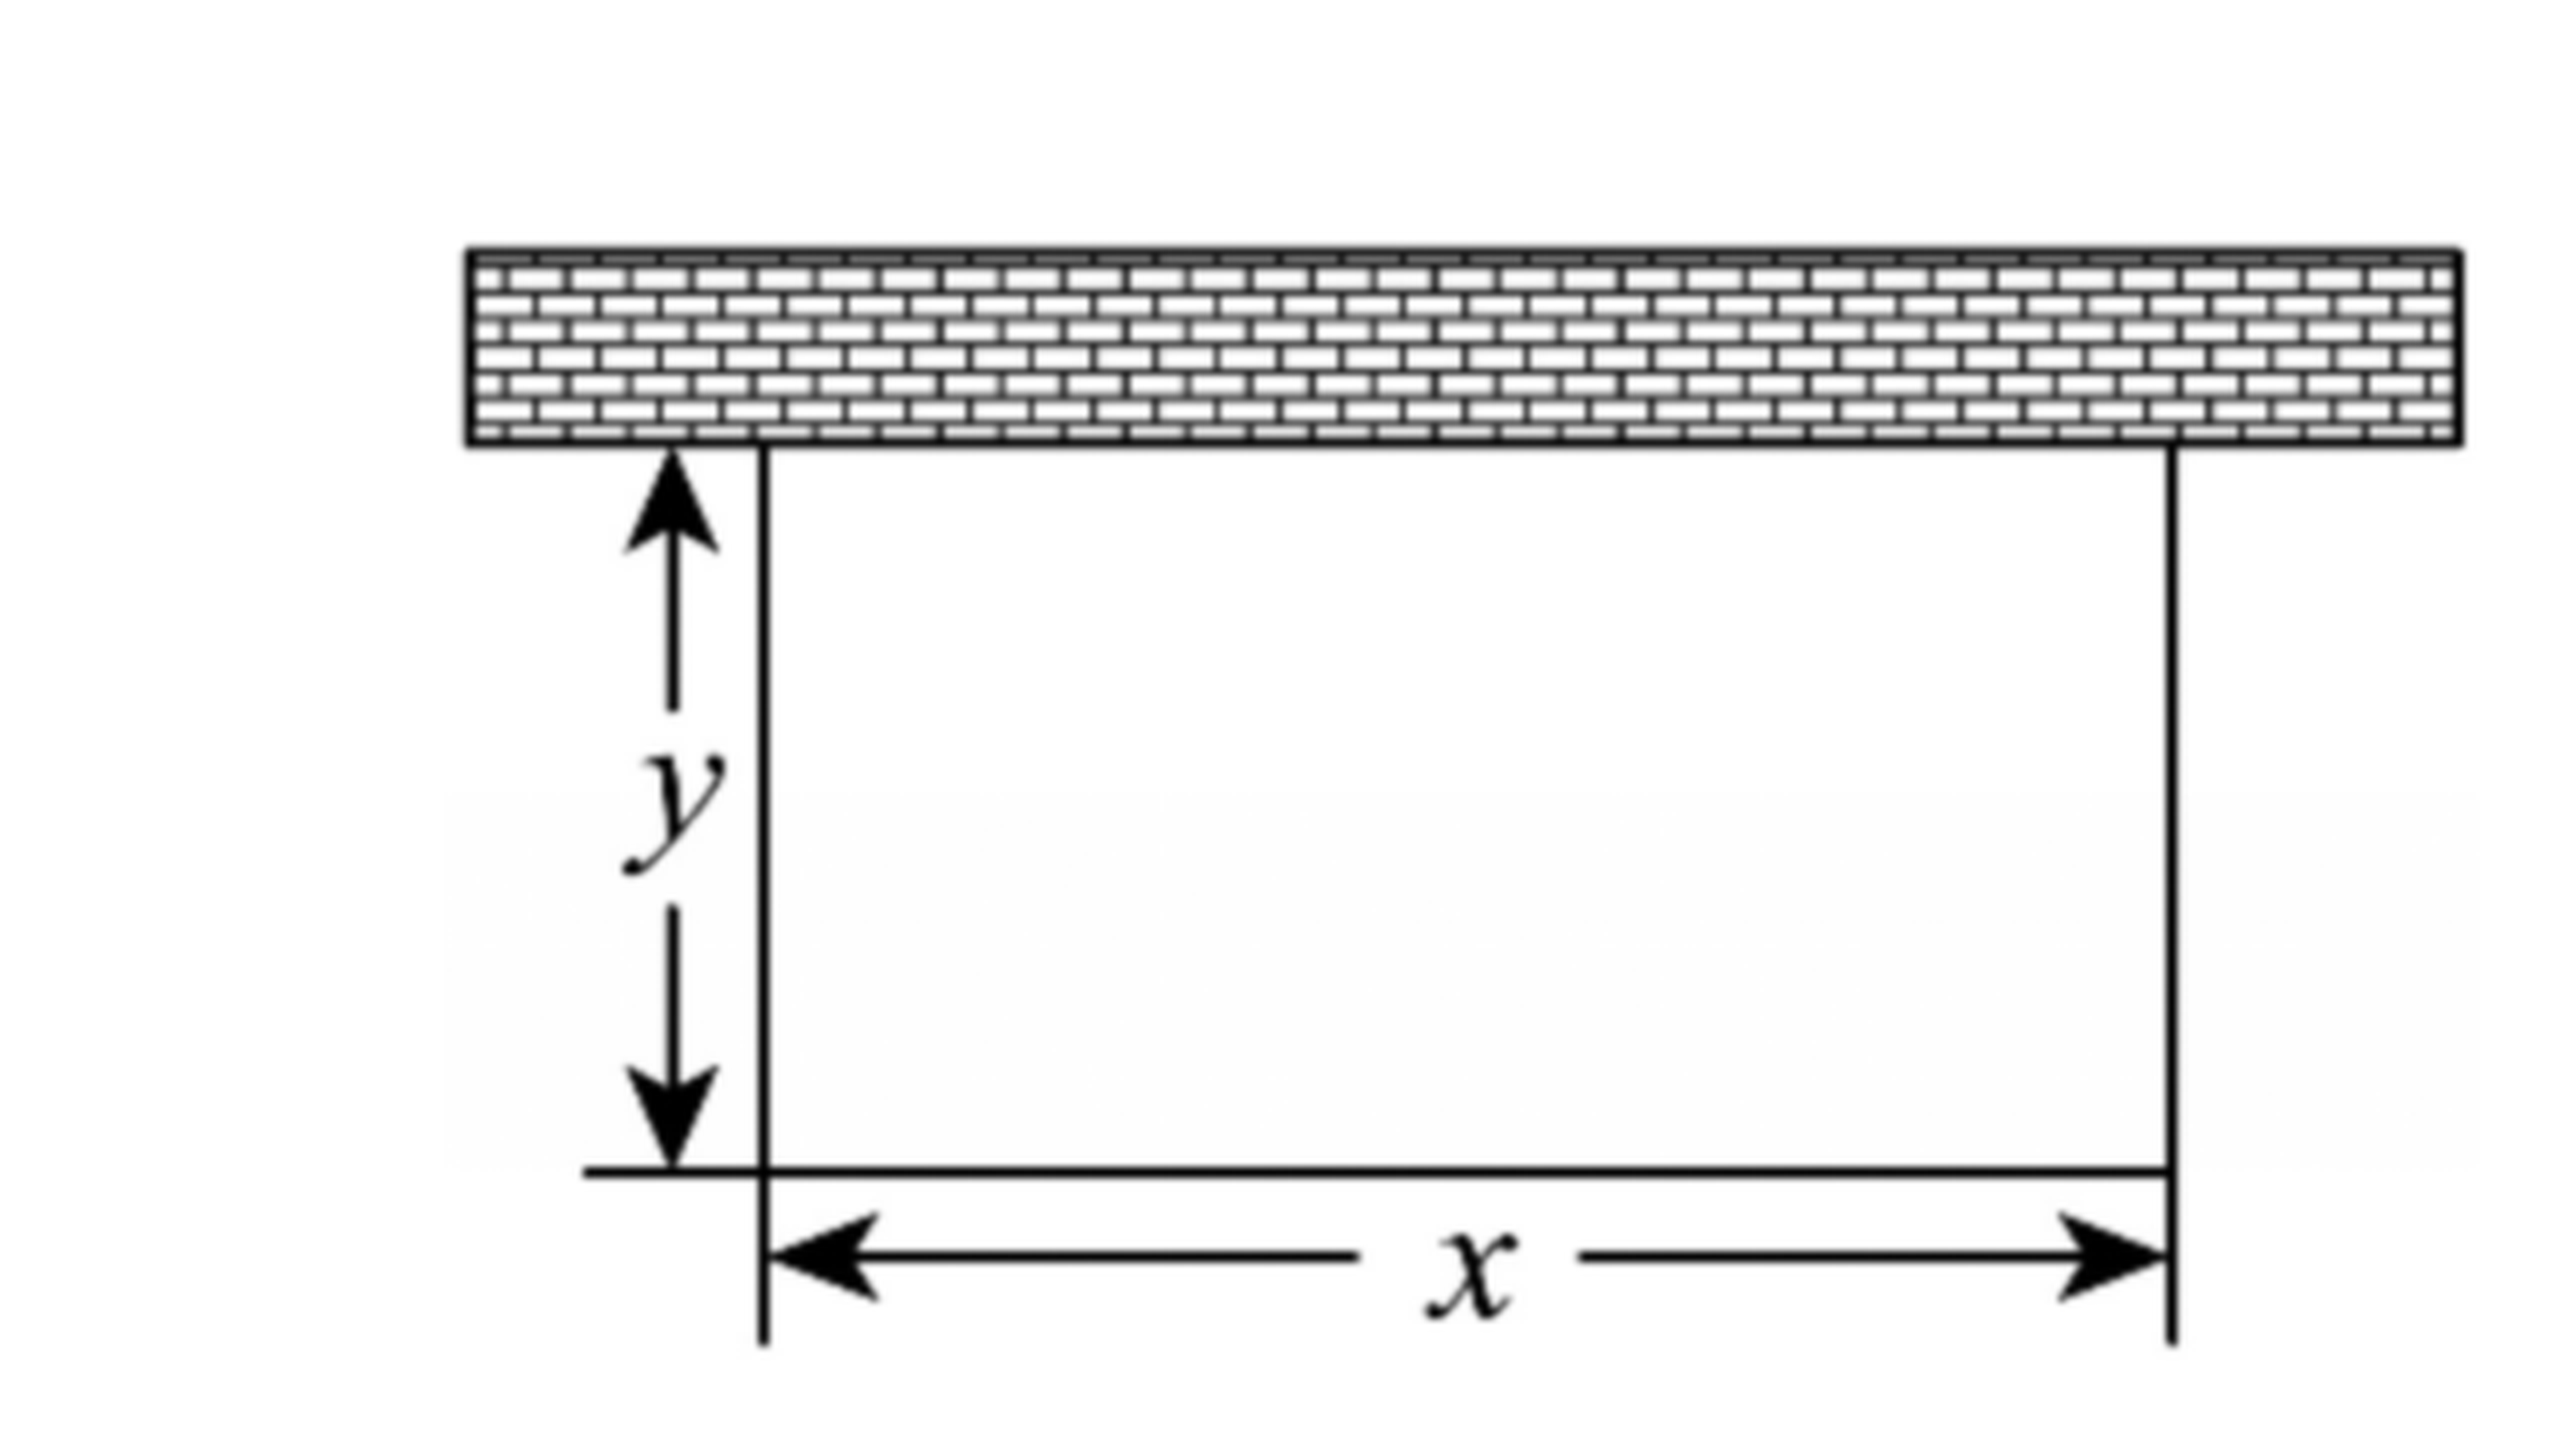
\includegraphics[width=0.55\textwidth]{figures/gao145_q20.png}
\end{center}

(1) 若菜园面积为 72 平方米，则 $x$、$y$ 为何值时，所用篱笆总长最小？

(2) 若 $x$、$y$ 满足 $x+y-xy+63=0$，则菜园面积最小为多少平方米？

\ifanswer
\solbegin
\step{(1) 由题意得，菜园的面积 $S=xy=72$，且 $x>0$，$y>0$，}
\step{所用篱笆总长 $L=x+2y$，}
\step{由基本不等式得 $x+2y\geqslant2\sqrt{x\cdot2y}=2\sqrt{2xy}=2\sqrt{2\times72}=24$，}
\step{当且仅当 $x=2y$ 时取等号，}
\step{联立 $\begin{cases}xy=72\\x=2y\end{cases}$，解得 $\begin{cases}x=12\\y=6\end{cases}$，}
\step{所以当 $x=12$，$y=6$ 时，所用篱笆总长最小；}
\step{(2) 由题意得 $x>0$，$y>0$，且满足 $x+y-xy+63=0$，即 $x+y=xy-63$，}
\step{由基本不等式得 $x+y\geqslant2\sqrt{xy}$，当且仅当 $x=y$ 时取等号，}
\step{所以 $xy-63\geqslant2\sqrt{xy}$. 令 $t=\sqrt{xy}(t>0)$，则 $xy=t^2$，}
\step{上述不等式可化为 $t^2-2t-63\geqslant0$，即 $(t-9)(t+7)\geqslant0$，}
\step{因为 $t>0$，所以 $t+7>0$，故 $t-9\geqslant0$，解得 $t\geqslant9$，所以 $\sqrt{xy}\geqslant9$，}
\step{即 $xy\geqslant81$，当且仅当 $x=y=9$ 时取等号，此时满足 $9+9-81+63=0$，}
\step{所以菜园面积最小为 81 平方米.}
\solend
\fi

% 第 21 题：题干在 10 页、解析续至 11 页（3 问、分类讨论很长），按印刷行断共 22 行；
% 末行"故第 2026 个元素是 2700 之后第一个属于 A 的数，即 2701." 为全卷收尾，
% 无 Q22/Q23、无附加题节；数集 Z/N* 按全稿惯例改 \Z/\N^*
\item 已知集合 $A=\{x\mid x=m^2-n^2$，$m$、$n\in\Z\}$.

(1) 求证：任何奇数 $2k+1(k\in\Z)$ 都是集合 $A$ 中的元素；

(2) 判断偶数 $4k-2(k\in\Z)$ 是否为集合 $A$ 的元素？请说明理由；

(3) 若将集合 $A$ 中的正整数由小到大排列，求出集合 $A$ 中第 2026 个正整数.

\ifanswer
\solbegin
\step{(1) 因为 $x=(k+1)^2-k^2=2k+1(k\in\Z)$，}
\step{所以任何奇数 $2k+1(k\in\Z)$ 都属于集合 $A$；}
\step{(2) 偶数 $4k-2(k\in\Z)$ 不是集合 $A$ 的元素，理由如下：}
\step{由题意得 $x=m^2-n^2=(m-n)(m+n)$，}
\step{当 $m$、$n$ 均为奇数时，设 $m=2k_1+1$，$n=2k_2+1(k_1$、$k_2\in\Z)$，}
\step{则 $m^2-n^2=(2k_1+1)^2-(2k_2+1)^2=(2k_1-2k_2)(2k_1+2k_2+2)$}
\step{$=4(k_1-k_2)(k_1+k_2+1)$，}
\step{因为 $k_1$、$k_2\in\Z$，所以 $k_1-k_2\in\Z$，$k_1+k_2+1\in\Z$，}
\step{从而 $m^2-n^2$ 为 $4$ 的倍数；}
\step{当 $m$、$n$ 均为偶数时，设 $m=2k_1$，$n=2k_2(k_1$、$k_2\in\Z)$，}
\step{$m^2-n^2=4k_1^2-4k_2^2=4(k_1^2-k_2^2)$ 为 $4$ 的倍数；}
\step{当 $m$、$n$ 为一个偶数一个奇数时，不妨设 $m$ 为偶数，$n$ 为奇数，}
\step{设 $m=2k_1$，$n=2k_2+1(k_1$、$k_2\in\Z)$，}
\step{则 $m^2-n^2=4k_1^2-(2k_2+1)^2=4(k_1^2-k_2^2-k_2)-1$ 为奇数.}
\step{无论哪种情况均不满足 $4k-2(k\in\Z)$，}
\step{故偶数 $4k-2(k\in\Z)$ 不是集合 $A$ 的元素；}
\step{(3) 由前两问得，$4$ 的倍数和奇数属于集合 $A$ 中的元素，}
\step{令集合 $A$ 中的正整数元素为 $4k-3$、$4k-1$、$4k(k\in\N^*)$，}
\step{对任意的 $k\in\N^*$，连续的 $4$ 个整数 $4k-3$、$4k-2$、$4k-1$、$4k$ 中}
\step{有三个数 $4k-3$、$4k-1$、$4k$ 都在集合 $A$ 中，}
\step{因为 $2026=3\times675+1$，所以集合 $A$ 中第 $2025$ 个元素为 $4\times675=2700$，}
\step{故第 2026 个元素是 2700 之后第一个属于 $A$ 的数，即 2701.}
\solend
\fi

\end{enumerate}

\end{document}
